\documentclass[colortheme=cyan]{transbook}
\usepackage[version=4]{mhchem}
\usepackage{makeidx}
\usepackage[acronym,symbols]{glossaries}
% \renewcommand*{\indexname}{函数索引}
\renewcommand*{\glossaryname}{词汇表}
\renewcommand*{\acronymname}{缩略语}
\makeindex
\makeglossaries
\setcounter{secnumdepth}{5}
\ctexset{
  subparagraph/number= \theparagraph\thinspace\alph{subparagraph},
}
% \setcounter{tocdepth}{2}
\DeclareMathOperator{\erf}{erf}
\renewcommand{\acrfullformat}[2]{#1(#2)}

%%% ----------------------------------------------------------------------------
%%% 自定义命令
%%% ----------------------------------------------------------------------------
\NewDocumentCommand{\bkn}{ s m }
	{\IfBooleanTF#1{\textit{#2}}{《#2》}}
\NewDocumentCommand{\msm}{}{ MSM\textsuperscript{\textregistered} }
\NewDocumentCommand{\lrfd}{}{\acrshort*{lrfd}~规范}
\NewDocumentCommand{\pontis}{}{Pontis\textsuperscript{\texttrademark}}
\NewDocumentCommand{\fluorogold}{}{Fluorogold\textsuperscript{\textregistered}}

\NewDocumentCommand\Microsoft{ o }
  {\textsf{Microsoft}\textsuperscript{\textregistered}\IfNoValueF{#1}{\thinspace #1}}
\NewDocumentCommand\Excel{o}{\textsf{Excel}\IfNoValueF{#1}{\thinspace #1}}
%%% ----------------------------------------------------------------------------
%%% 词汇表与缩略语
%%% ----------------------------------------------------------------------------
\newglossaryentry{element}{%
  name = 构件,
  sort = gou4jian4,
  description = {单独的桥梁构件,例如主梁、底梁、纵梁、盖梁、支座、伸缩缝、栏杆等。结合起来,这些\gls{element}形成\gls{subsystem}和\gls{component},然后构成桥梁\gls{system}}
}
\newglossaryentry{component}{%
  name = 组件,
  sort = zu3jian4,
  description = {桥梁\gls{element}的组合,形成构成整个桥梁结构的三个主要部分之一。桥梁\gls{system}的三个主要\gls{component}是下部结构、上部结构和桥面系}
}
\newglossaryentry{subsystem}{%
  name = 子系统,
  sort = zi3xi4tong3,
  description = {两个或多个桥梁\gls{element}的组合,共同作用以服务于共同的结构  目的。示例包括组合梁,它可以由梁、钢筋和混凝土组成}
}
\newglossaryentry{system}{%
  name = 系统,
  sort = xi4tong3,
  description = {桥梁的三大\gls{component}——桥面系、下部结构和上部结构——结合在一起形成一个完整的桥梁}
}

\newglossaryentry{servicelife}{%
  name = 使用寿命,
  sort = shi3yong4shou4ming4,
  description = {桥梁\gls{element}、\gls{component}、\gls{subsystem}或\gls{system}提供所需性能或功能水平以及任何所需水平的维修和/或维护的持续时间}
}
\newglossaryentry{targetdesignservicelife}{%
  name = 目标设计使用寿命,
  sort = mu4biao1she4ji4shi3yong4shou4ming4,
  description = {预计桥梁\gls{element}、\gls{component}、\gls{subsystem}和\gls{system}将提供所需功能并在设计或改造阶段建立指定维护水平的持续时间}
}
\newglossaryentry{designlife}{%
  name = 设计寿命,
  sort = she4ji4shou4ming4,
  description = {为确定可变作用的取值而取用的统计意义上的时间参数}
}
\newglossaryentry{life365}{%
  name = {Life-365\textsuperscript{\texttrademark}},
  description = {一款旨在估算混凝土配合比设计方案的使用寿命和生命周期成本的软件}
}
% \newglossaryentry{}{%
%   name = ,
%   sort = ,
%   description = {}
% }
%%%-----------------------------------------------------------------------------
%%% 翻译用词
%%%-----------------------------------------------------------------------------
\newglossaryentry{obsolescence}{%
  name = 陈旧,
  type = symbols,
  description={}
}
\newglossaryentry{deterioration}{%
  name = 劣化,
  type = symbols,
  description={}
}
\newglossaryentry{faulttree}{%
  name = 故障树,
  type = symbols,
  description={}
}
\newglossaryentry{workzone}{%
  name = 施工影响区,
  type = symbols,
  description={}
}
\newglossaryentry{adjacentbox}{%
  name = 多片梁式结构,
  type = symbols,
  description={}
}
% \newglossaryentry{}{%
%   name = ,
%   type = symbols,
%   description={}
% }
%%%-----------------------------------------------------------------------------
%%% 缩略语
%%%-----------------------------------------------------------------------------
\newacronym[%
  description={National Steel Bridge Alliance, 全国钢桥联盟}
]{nsba}{NSBA}{全国钢桥联盟}

\newacronym[%
  description={Long-Term Bridge Performance, 长期桥梁性能}
]{ltbp}{LTBP}{长期桥梁性能}

\newacronym[%
  description={Geosynthetic Reinforced Soil Integrated Bridge System, 土工合成材料加筋土整体桥梁系统}
]{grsibs}{GRSIBS}{土工合成材料加筋土整体桥梁系统}

\newacronym[%
  description={Mechanically-Stabilized Earth, 机械稳定土}
]{mse}{MSE}{机械稳定土}

\newacronym[%
  description={Peak Ground Acceleration, 地表加速度峰值}
]{pga}{PGA}{地表加速度峰值}

\newacronym[%
  description={University of Nebraska–Lincoln, 内布拉斯加大学林肯分校}
]{unl}{UNL}{内布拉斯加大学林肯分校}

\newacronym[%
  description={Simple for Dead Load and Continuous for Live Load, 恒载简支活载连续}
]{sdcl}{SDCL}{恒载简支活载连续}

\newacronym[%
  description={United States Office of Management and Budege, 美国行政管理和预算局}
]{omb}{OMB}{美国行政管理和预算局}

\newacronym[%
  description={Analytical Hierarchy Process, 层次分析法}
]{ahp}{AHP}{层次分析法}

\newacronym[%
  description={National Institute of Standards and Technology, 美国国家标准技术研究院}
]{nist}{NIST}{美国国家标准技术研究院}

\newacronym[%
  description={Average Daily Truck Traffic, 日平均卡车交通量}
]{adtt}{ADTT}{日平均卡车交通量}

\newacronym[%
  description={Average Annual Daily Traffic, 年平均日交通量}
]{aadt}{AADT}{年平均日交通量}

\newacronym[%
  description={vehicle operating costs, 车辆运营成本}
]{voc}{VOC}{车辆运营成本}

\newacronym[%
  description={Present Value, 现值}
]{pv}{PV}{现值}

\newacronym[%
  description={Net Present Value, 净现值}
]{npv}{NPV}{净现值}

\newacronym[%
  description={Service Life, 使用寿命}
]{sl}{SL}{使用寿命}

\newacronym[%
  description={Accelerated Bridge Construction, 快速桥梁建造}
]{abc}{ABC}{快速桥梁建造}

\newacronym[%
  description={Benefit-Cost Analysis, 效益成本分析}
]{bca}{BCA}{效益成本分析}

\newacronym[
  description={Allowable Stress Design, 容许应力设计}
]{asd}{ASD}{容许应力设计}

\newacronym[
  description={Load Factor Design, 荷载系数设计}
]{lfd}{LFD}{荷载系数设计}

\newacronym[%
  description = {Department of Transportation, 交通部}
]{dot}{DOT}{交通部}

\newacronym[
  description={Polytetrafluorethylene, 聚四氟乙烯}
]{ptfe}{PTFE}{聚四氟乙烯}

\newacronym[%
  description={Cotton Duck Pad,在美国采用的一种简易的弹性支座类型,姑且按原文直译为\acrlong{cdp},感觉和国内使用的油毛毡类似}
]{cdp}{CDP}{棉鸭垫}

\newacronym[%
  description={Alkali Aggregate Reaction, 碱骨料反应}
]{aar}{AAR}{碱骨料反应}

\newacronym[%
  description={Cast-In-Place, 现场浇筑}
]{cip}{CIP}{现场浇筑}

\newacronym[%
  description={American Society for Testing and Materials, 美国材料与试验学会}
]{astm}{ASTM}{美国材料与试验学会}

\newacronym[%
  description={American Association of State Highway and Transportation Officials, 美国国家公路和运输官员协会}
]{aashto}{AASHTO}{美国国家公路和运输官员协会}

\newacronym[%
  description={American Concrete Institute, 美国混凝土协会}
]{aci}{ACI}{美国混凝土协会}

\newacronym[%
  description={Alkali-Carbonate Reaction, 碱—碳酸盐反应}
]{acr}{ACR}{碱—碳酸盐反应}

\newacronym[%
  description={Air Entrained, 引气}
]{ae}{AE}{引气}

\newacronym[%
  description={Normal Weight Concrete, 普通重量混凝土}
]{nwc}{NWC}{普通重量混凝土}

\newacronym[%
  description={Light Weight Concrete, 轻质混凝土}
]{lwc}{LWC}{轻质混凝土}

\newacronym[%
  description={Fiber-Reinforced , 纤维增强混凝土}
]{frc}{FRC}{纤维增强混凝土}

\newacronym[%
  description={High Performance Concrete, 高性能混凝土}
]{hpc}{HPC}{高性能混凝土}

\newacronym[%
  description={Ultra-High Performance Concrete, 超高性能混凝土}
]{uhpc}{UHPC}{超高性能混凝土}

\newacronym[%
  description={Self-Consolidating Concrete, 自密实混凝土}
]{scc}{SCC}{自密实混凝土}

\newacronym[%
  description={Normal Weight Aggregates, 普通重量骨料}
]{nwa}{NWA}{普通重量骨料}

\newacronym[%
  description={LightWeight Aggregates, 轻骨料}
]{lwa}{LWA}{轻骨料}

\newacronym[%
  description={Alkali-Silica Reaction, 碱硅反应}
]{asr}{ASR}{碱硅反应}

\newacronym[%
  description={Federal Highway Administration, 联邦公路管理局}
]{fhwa}{FHWA}{联邦公路管理局}

\newacronym[%
  description={ F\'ed\'eration Internationale du B\'eton (International Federation for Structural Concrete), 国际混凝土联合会}
]{fib}{\textbf{\itshape fib}}{国际混凝土联合会}

\newacronym[%
  description={Ground Granulated Blast Furnace Slag, 研磨粒状高炉矿渣}
]{ggbs}{GGBS}{研磨粒状高炉矿渣}

\newacronym[%
  description={Fiber Reinforced Polymer, 纤维增强复合材料}
]{frp}{FRP}{纤维增强复合材料}

\newacronym[%
  description={International Organization for Standardization, 国际标准化组织}
]{iso}{ISO}{国际标准化组织}

\newacronym[%
  description={Life Cycle Cost Analysis, 全生命周期成本分析}
]{lcca}{LCCA}{全生命周期成本分析}

\newacronym[%
  description={Life Cycle Cost, 全生命周期成本}
]{lcc}{LCC}{全生命周期成本}

\newacronym[%
  description={Load and Resistance Factor Design, 荷载—抗力系数设计}
]{lrfd}{LRFD}{荷载—抗力系数设计}

\newacronym[%
  description={National Cooperative Highway Research Program, 国家公路合作研究计划}
]{nchrp}{NCHRP}{国家公路合作研究计划}

\newacronym[%
  description={Ordinary Portland Cement, 普通波特兰水泥}
]{opc}{OPC}{普通波特兰水泥}

\newacronym[%
  description={Supplementary Cementitious Material, 辅助胶凝材料}
]{scm}{SCM}{辅助胶凝材料}

\newacronym[%
  description={Strategic Highway Research Program, 公路研究战略计划}
]{shrp}{SHRP}{公路研究战略计划}

\newacronym[%
  description={Water-to-CeMent ratio, 水灰比}
]{wcm}{WCM}{水灰比}

\newacronym[%
  description={High-Load Multi-Rotation, 大吨位多向转动}
]{hlmr}{HLMR}{大吨位多向转动}

\newacronym[%
  description={Epoxy-Coated Reinforcement, 环氧涂层钢筋}
]{ecr}{ECR}{环氧涂层钢筋}

\newacronym[%
  description={Constant-Amplitude Fatigue Limit, 等幅疲劳极限}
]{cafl}{CAFL}{等幅疲劳极限}

\newacronym[%
  description={Constant-Amplitude Fatigue Threshold, 等幅疲劳阈值}
]{caft}{CAFT}{等幅疲劳阈值}

\newacronym[%
  description={Linear Elastic Fracture Mechanics, 线弹性断裂力学}
]{lefm}{LEFM}{线弹性断裂力学}

\newacronym[%
  description={Plastic Fracture Mechanics, 塑性断裂力学}
]{pfm}{PFM}{塑性断裂力学}

\newacronym[%
  description={High Range Water Reducing Admixtures, 高范围减水外加剂}
]{hrwra}{HRWRA}{高范围减水外加剂}

\newacronym[%
  description={Visual Stability Index, 视觉稳定系数}
]{vsi}{VSI}{视觉稳定系数}

\newacronym[%
  description={Poly-Vinyl Alcohol, 聚乙烯醇}
]{pva}{PVA}{聚乙烯醇}

%%% ----------------------------------------------------------------------------  %% 自定义设置,包括词汇表和缩略语
%%% 参考文献设置
\usepackage[backend=biber, 
  style=gb7714-2015ay, 
  % gbalign=gb7714-2015, 
  natbib=true,isbn,
  gbannote=true,
  gbpub=false]{biblatex}
\def\UrlFont{\ttfamily}  %% 恢复 url 的字体样式
\addbibresource[location=local]{R19A.bib}

%%% 图书元数据的设置
\Booksetup{
  BookTitle   = 桥梁使用寿命设计指南,
  BookTitle*  = Design Guide for Bridge for Service Life,
  BriefIntro    = 
    { 
      本书的重点是北美的设计实践,并为混凝土和钢结构的公路桥梁提供使用寿命设计原则的应用参考。该文档介绍了使用寿命设计、使用寿命设计过程以及使用寿命设计的不同概念。可供桥梁业主和设计师可以使用它来提高使用本文档中包含的方法和参考建造的桥梁的性能。
    },
  CoverGraph    = graphics/cvgraph.png,
  AuthorList*   = {Atorod Azizinamini, Edward H. Power, Glenn F. Myers, H. Celik Ozyildirim},
  AuthorList    = {张晨南}, 
  WrittenStyle  = 译,
}

%%% 正文

\begin{document}
\frontmatter
\tableofcontents
\listoffigures
\listoftables
\cleardoublepage 
\phantomsection\addcontentsline{toc}{chapter}{词汇表}
\printglossary[nonumberlist]
\cleardoublepage
\phantomsection\addcontentsline{toc}{chapter}{缩略语}
\printacronyms[nonumberlist]
\mainmatter
% \chapter{Design for Service Life: General Framework}
\chapter{\glsentrytext{servicelife}设计 — 总体框架}
\label{chp:general-frame}
% The design for service life is gaining more importance as limited resources demand enhancing the service life of existing and new bridges. As part of the research project entitled \bkn*{Bridges for Service Life Beyond 100 Years:c Innovative Systems, Subsystems and Components} and supported by \acrshort{sharp} \emph{Project R19A}, a systematic and general approach to design for service life has been developed. The major product of this project is this document, referred to as \bkn*{Design Guide for Bridges for Service Life}, hereafter referred to as the \bkn*{Guide}. This chapter provides the general framework used in the Guide, primarily for bridges with spans of less than about \qty{300}{ft}. However, the framework is general and can be adapted and customized for major and complex bridges such as those with much longer spans. It can also be adapted to suit bridges located in any region within the United States, recognizing however, that while the framework remains the same for all bridges, the resulting details for service life could be significantly different.
人们已经意识到由于资源的有限而需要提高既有桥梁和新建桥梁的\gls*{servicelife},这使得\gls*{servicelife}设计变得越来越重要。作为题为\bkn{\gls*{servicelife}超过 100 年的桥梁:创新系统、子系统与组件}\footnote{标题原文\bkn*{Bridges for Service Life Beyond 100 Years: Innovative Systems, Subsystems and Components}}研究项目的一部分,在\acrfull{shrp}的 R19A 项目的支持下,一种系统的、通用的\gls*{servicelife}设计方法被开发了出来。本项目的主要成果是这本\bkn{桥梁\gls*{servicelife}设计指南}\footnote{标题原文\bkn*{Design Guide for Bridges for Service Life}},以下简称\bkn{指南}。本章提供\bkn{指南}中使用的总体框架,主要用于跨度小于 \qty{90}{m} 的桥梁。然而,该框架是通用的,可以针对大型和复杂的桥梁(例如跨度更大的桥梁)进行调整和定制。它可以适用于位于美国任何地区的桥梁,但是要认识到,虽然对于所有桥梁来说,\gls*{servicelife}设计的框架都是相同,但由此产生的有关\gls{servicelife}的细节可能会大不相同。

% \section{Background}
\section{背景}
% Providing safety for the public by having adequate strength for constructed facilities has been the cornerstone of the framework used by engineers for bridge design. This design for strength approach has not been restricted to bridges---it has also been the framework one could find in various building codes. In the case of buildings, however, most structural elements are protected from environmental-type loads and as a result the strength framework has served this sector of the industry very well. In the case of bridges or pavements, which are constructed facilities exposed to environmental loads, the story is different.
建造能提供足够强度的设施来保障公共安全,这一直是工程师用于桥梁设计的基石。这种强度设计方法并不仅限于桥梁——在各种建筑规范中也可以找到相应的框架。就建筑物而言,大多数结构构件都能得到保护而不受自然环境荷载的影响,因此强度设计方法的框架非常适合该行业。然而,对于暴露在自然环境中承受各种环境荷载的桥梁或人行道,情况就有所不同了。

% Significant changes to our contemporary bridge design specifications have also been mainly related to strength issues. The transitions from Allowable Stress Design (ASD) to Load Factor Design (LFD), and more recently to the Load and Resistance Factor Design (LRFD), reflect this line of thinking. It is also important to note that in the early 1970s, bridge engineers developed criteria for steel bridge details to protect against fatigue and fracture failure. These were indeed service life design provisions.
我们当代桥梁设计规范的重大变化也主要与强度问题有关。从\acrfull{asd}到\acrfull{lfd},以及近来向\acrlong{lrfd}的转变,反映了这种思路。同样需要指出的是,在 20 世纪 70 年代初期,桥梁工程师制定了钢桥细节标准以防止疲劳和断裂失效。这些其实也是\gls*{servicelife}设计规定的范畴。

% The strength framework did not prevent visionary engineers such as John Roebling to think in terms of service life. A review of bridges that have lasted more than 100 years provides valuable lessons. These bridges are not so much innovative in system or material, but have proven to be:
% \begin{itemize}
%   \item Maintainable and well maintained over their 100-year lives due to extreme importance or high capital replacement cost,
%   \item Adaptable to changes in functional use as well as service limit state demands and/or,
%   \item Originally overdesigned.
% \end{itemize}
强度设计方法的框架并没有阻止 \pnme{John Roebling} 等有远见的工程师从\gls*{servicelife}的角度思考问题。回顾历经 100 多年风雨的桥梁可以获得宝贵的经验教训。这些桥梁在体系或材料上并没有太多创新,之所以能历经百年,已被证明的因素是:
\begin{itemize}
  \item 由于桥梁本身极其重要或替换重建成本太高,因而设计考虑了在 100 年\gls{servicelife}内结构的可维护性,且结构也得到了良好的维护;
  \item 桥梁对于使用功能的变化和服务极限状态需求有比较强的适应性;
  \item 桥梁从一开始就进行了过度设计。
\end{itemize}

% Examples of bridges with long service lives are New York City's oldest East River bridges, the Brooklyn Bridge (the longest bridge in the world when opened to traffic in 1883) and the Williamsburg Bridge (the longest bridge in the world when opened in 1903), and St. Louis's Eads Bridge (the first steel bridge opened in 1874).
\gls*{servicelife}较长的桥梁例子有纽约市最古老的东河上的桥梁,如布鲁克林大桥(Brooklyn Bridge,1883 年通车时是世界上最长的桥梁),威廉斯堡大桥(Williamsburg Bridge,1903 年通车时是世界上最长的桥梁),和圣路易斯的伊兹桥(Eads Bridge,1874 年开通的第一座钢桥)。

% The Brooklyn Bridge has been well maintained and rehabilitated in a timely manner throughout its lifetime. Initial coatings to protect the bridge's steel from corrosion did not provide a 100-year life, but cleaning and repainting the bridge did. The metal deck of the Brooklyn Bridge has not survived its 100 plus year service life, but replacement of the replaceable metal decking has. \Cref{fig:brooklyn-bridge} shows the Brooklyn Bridge circa 1890.
布鲁克林大桥在其整个生命周期内都得到了及时的维护和修复。仅仅靠防腐涂层来保护桥梁钢材并不能保证 100 年的\gls*{servicelife},但清理和重新涂装桥梁就能够做到这一点。布鲁克林大桥的钢桥面并没有达到 100 多年的\gls*{servicelife},但对钢桥面进行更换后就达到了这一目标。 \cref{fig:brooklyn-bridge} 展示了大约 1890 年的布鲁克林大桥。

\begin{figure}
  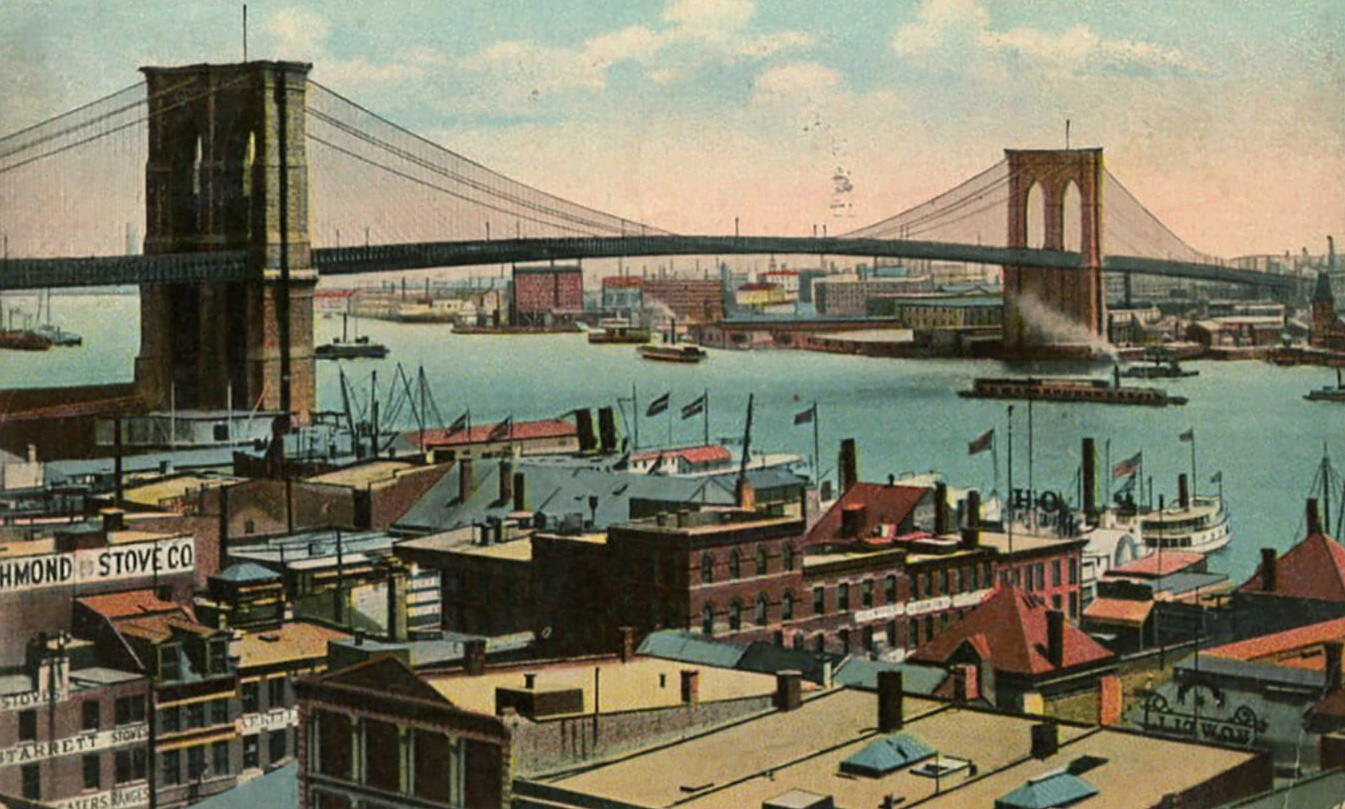
\includegraphics[width=0.9\linewidth]{brooklyn-bridge.jpg}
  % \caption{The Brooklyn Bridge from the South Street Seaport, circa 1890.}
  \caption{从南街海港处看到的布鲁克林大桥(1890 年左右)}
  \label{fig:brooklyn-bridge}
\end{figure}

% The Williamsburg Bridge was not as well maintained as evidenced by its mergency closing in 1988. In April of that year, after a thorough inspection revealed corrosion of the cables, beams and steel supports, the Williamsburg Bridge was closed to all vehicular and train traffic for nearly two months. After engineers performed emergency construction on the bridge and reopened it to traffic, a panel of design experts convened to determine if the Williamsburg Bridge should be replaced, or if it should be rehabilitated. In November 1988, after evaluating several alternatives, the New York City Department of Transportation (DOT) determined that the Williamsburg Bridge should be repaired while kept open to traffic. This option was deemed to have the least detrimental impact on motorists and nearby communities. In 1991, the New York City DOT began a major rehabilitation of the Williamsburg Bridge. The program  was designed to undo the effects of age, weather, increased traffic volumes, and deferred maintenance. \Cref{fig:williamsburg-bridge} shows the Williamsburg Bridge circa 1904.
威廉斯堡大桥在 1988 年进行紧急关闭,这表明其维护得并不好。当年 4 月,在经过彻底检查发现主缆、横梁和钢支承有所腐蚀后,威廉斯堡大桥对所有汽车和火车关闭交通将近两个月。在工程师对桥梁进行紧急施工并重新开放交通后,一个设计专家小组召开会议,以确定是否应该更换威廉斯堡大桥,或者对其进行修复。1988 年 11 月,在评估了几种备选方案后,纽约市\acrfull{dot}决定修复威廉斯堡大桥,同时保持交通畅通。该选项被认为对驾车者和附近社区的不利影响最小。1991 年,纽约市\acrlong{dot}开始启动对威廉斯堡大桥进行大规模修复的计划,该计划旨在消除结构老化、天气、交通量增加和维护延期的影响。 \cref{fig:williamsburg-bridge} 显示了大约 1904 年的威廉斯堡大桥。

\begin{figure}
  \centering
  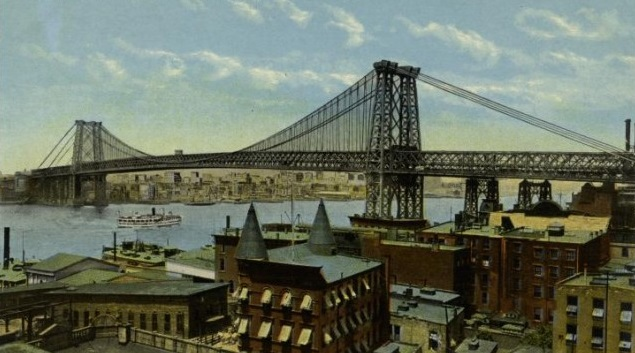
\includegraphics[width=0.9\linewidth]{williamsburg-bridge.jpg}
  % \caption{The Williamsburg Bridge, circa 1904.}
  \caption{威廉斯堡大桥(1904 年左右)}
  \label{fig:williamsburg-bridge}
\end{figure}

% The decision to rehabilitate the Williamsburg Bridge instead of undertaking a costly in-place replacement in downtown Manhattan was made possible by the original conservative design of the bridge cables. The need to rehabilitate the cable was necessitated by a poor corrosion-protection choice. Leffert~L. Buck, the designer of the Williamsburg Bridge, chose linseed oil. The 1988 inspection of the Williamsburg Bridge cables revealed significant corrosion, proving the choice of linseed oil to be a relatively poor one. For the Brooklyn Bridge, John Augustus Roebling chose a coating of graphite to protect the individual wires of the bridge cable from corrosion, a choice that provided over 100 years of corrosion protection. Fortunately, the cable design for the Williamsburg Bridge utilized a factor of safety of resistance divided by load of about 5. After the significant loss of section due to corrosion was observed in 1988, the factor of safety was deemed adequate and a cable rehabilitation program to arrest the corrosion was initiated instead of a cable replacement. Thus, original overdesign allowed the bridge and its cables to continue in service.
威廉斯堡大桥采取了修复的方式而不是在曼哈顿市中心进行昂贵的就地更换,这项决定之所以具有可行性,其原因在于桥梁主缆最初采用了保守设计。由于防腐体系的选择不当,主缆需要进行修复。威廉斯堡大桥的设计者 \pnme{Leffert~L. Buck} 在主缆防腐上选择了亚麻籽油。 1988 年对威廉斯堡大桥主缆的检查发现有明显的腐蚀,证明亚麻籽油的选择是一个相对较差的选择。而像布鲁克林大桥,\pnme{John Augustus Roebling} 选择了石墨涂层来保护桥梁主缆的单根钢丝免受腐蚀,这种方案就提供了长达 100 多年的腐蚀保护。幸运的是,威廉斯堡大桥的主缆设计采用了抗力与荷载之比为 5 左右的安全系数。即使在 1988 年观察到由于腐蚀造成的截面显著损失后,其安全系数也被认为是足够的,这样,防止腐蚀的主缆修复计划得以启动,桥梁并没有更换主缆。因此,实际上是最初的过度设计允许桥梁及其主缆继续使用。

% The Eads Bridge, completed in 1874 and named for its designer and builder, James Buchanan Eads, has proven long-lived by being well maintained and readily adaptable. \Cref{fig:eads-bridge} shows the Eads Bridge circa 1983. The scale of the bridge was unprecedented: the more than 500-ft span of the center arch exceeded by some \qty{200}{ft} any arch built previously. The arch ribs were made of steel, its first extensive use in a bridge. An additional innovation was the cantilever erection of the arches without falsework, the first example of this type of construction for a major bridge.

伊兹桥于 1874 年完工,并以其设计师和建造者 \pnme{James Buchanan Eads} 的名字命名,由于自身良好的适应性且经过良好维护,它经久不衰。 \cref{fig:eads-bridge} 显示了大约 1983 年的伊兹桥。这座桥的规模是前所未有的:中心拱 \qty{150}{m} 的跨度超过了以往建造的任何一座拱桥的拱肋跨度(\qty{60}{m}左右)。拱肋采用了桥梁中的首次使用的钢结构拱肋。另一项创新是在无支架的情况下悬臂架设主拱,这是采用此类施工方法建设大型桥梁的第一个例子。

\begin{figure}
  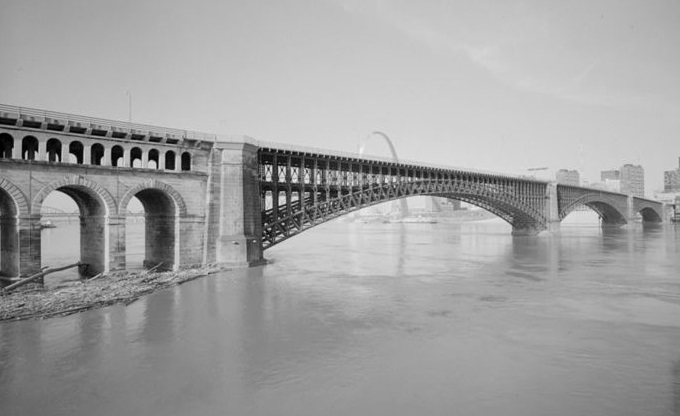
\includegraphics[width=0.9\linewidth]{eads-bridge.jpg}
  % \caption{The Eads Bridge looking toward St. Louis and the Gateway Arch, circa 1983.}
  \caption{向圣路易斯和拱门方向望去的伊兹桥(1983 年左右)}
  \label{fig:eads-bridge}
\end{figure}

% An interesting feature of the history of the Eads Bridge has been its adaptability to varying use. (It should be noted that the Brooklyn and Williamsburg Bridges have also seen varied use.) The bridge was originally a railway bridge carrying pedestrians on an upper deck with two rail lines below. The Eads Bridge eventually carried vehicular and rail traffic and the last train crossed the bridge in 1974. By the early 1990s, traffic on the bridge had dwindled to about \num{4000} cars a day and in 1991, the Eads Bridge was closed. For a while, it was unused altogether, but in 1993, new uses were found. MetroLink, the region's new light rail system, began to use the lower deck, which originally served passenger and freight train traffic and in 2003, the upper deck reopened to buses and automobiles. Today, a new lane for pedestrians and bicyclists on the south side of the bridge provides a great place to look at the river and the skyline of the city.
有关伊兹桥历史上的一个有趣特征是它对不同用途的适应性。(应该指出的是,布鲁克林大桥和威廉斯堡大桥也有不同的用途。)这座桥最初是一座铁路桥,上层载有行人,下面有两条铁路线。伊兹桥实际上最终承载了车辆和铁路交通,直到最后一列火车于 1974 年通过了这座桥。到 1990 年代初,桥上的交通量减少到每天约 \num{4000} 辆汽车,到了 1991 年,伊兹桥关闭。此后有一段时间内,它完全没有被使用,直到 1993 年,发现了新的用途。该地区的新轻轨系统 MetroLink 开始使用最初服务于客运和货运列车交通的下层,到了 2003 年,上层重新向公共汽车和汽车开放。如今,大桥南侧的行人和自行车道成为了观赏河流和城市天际线的绝佳场所。

% The examples of these three 100-plus yr old bridges illustrates that for bridges to serve a long life, they must be:
这三座历经 100 多年的老桥的例子说明,要使桥梁\gls*{servicelife}更长久,它们必须是:
\begin{itemize}
  % \item Resistant to environmental and man-made hazards,
  \item 具有抵抗环境和人为危害的能力;
  % \item Maintainable (and subsequently maintained) or relatively maintenance-free, and
  \item 具有可维护性(并在随后切实维护)或具有相对免维护性;
  % \item Adaptable to changes in traveled-way cross section and usage.
  \item 对行车道断面和使用用途的变化具有一定的适应性。
\end{itemize}

% Traditional approaches for enhancing the service life of bridges used in various codes and specifications such as AASHTO specifications, Eurocodes, or British Standards, are mainly in an indirect form, specifying the use of certain details or properties such as cover thickness, maximum crack width, concrete compressive strength, etc.
\acrshort{aashto} 规范、欧洲规范或英国标准等各种规范中使用的提高桥梁\gls*{servicelife}的传统方法主要采用间接方式,即指定使用某些细节或属性,例如保护层厚度、最大裂缝宽度、混凝土抗压强度等。

% Recognizing the importance of design for service life has motivated different agencies to undertake new initiatives for developing more formal design approaches for service life, similar to those used for design for strength. However, to date the majority of these efforts have concentrated on addressing concrete durability and service life, and significant advances have been achieved in this field. Designing bridges for service life, however, is more than just addressing service life and durability of concrete.

认识到\gls*{servicelife}设计的重要性促使不同的机构采取新的举措来开发更正式的\gls{servicelife}设计方法,类似于用于强度设计的方法。迄今为止,这些努力中的大部分都集中在解决混凝土的耐久性和\gls*{servicelife}问题上,并且在该领域已经取得了重大进展。然而,为\gls*{servicelife}设计桥梁不仅仅是解决混凝土的\gls*{servicelife}和耐久性问题。

% Furthermore, the design for service life for bridges needs to be approached in a systematic, all-inclusive manner rather than as a series of isolated tasks, each addressing service life of a particular portion of a bridge independently. The interaction between strategies for enhancing the service life of different bridge elements, components, and subsystems must be given critical consideration. In addition, a maintenance program, retrofit or replacement options, and management plan should all be part of this systematic service life design approach. In summary, at the design stage the design for service life should be approached as a comprehensive plan capable of providing the owner with a complete picture of what will be necessary for the bridge to achieve its specified service life.
此外,桥梁的\gls*{servicelife}设计需要以系统的、包罗万象的方式进行,而不是作为一系列孤立的任务,每个任务都独立地处理桥梁特定部分的\gls*{servicelife}。必须严格考虑提高不同桥梁\gls*{element}、\gls*{component}和\gls*{subsystem}\gls*{servicelife}的措施之间的相互作用。此外,维护计划、改造或更换选项以及管理计划都应该是该系统\gls*{servicelife}设计方法的一部分。总而言之,在设计阶段,\gls*{servicelife}设计应作为一个综合计划来处理,该计划能够为业主提供一个完整的画面,说明桥梁达到其指定\gls*{servicelife}所需的条件。

% The most notable efforts to develop a scientific approach for service life and durability of concrete elements (covering buildings, bridges, and tunnels) were a series of studies carried out between 1996 and 1999 in Europe for the fédération international du béton (The International Federation for Structural Concrete). One of the products of these efforts was the publication of \textbf{\em fib} \bkn{Bulletin 34}, \emph{Model Code for Service Life Design}, (TTD 2006). \emph{Bulletin 34}, however, only concentrated on addressing concrete service life and durability. Further, caution must be exercised when applying the recommendations of this publication to concrete placed in a horizontal configuration, such as a bridge decks. While \emph{Bulletin 34} has many useful recommendations for designing concrete elements for service life and  durability, the application of these recommendations to bridge components such as bridge decks remains a point of debate (in particular the use of various solutions to Fick's second law to predict the rate of chloride ingress through deck concrete). The use of recommendations made in \emph{Bulletin 34} is believed to be most applicable for concrete in vertical configuration and under compression, such as in substructure columns or sides of concrete box girders. This same debate can also be extended to the use of some of the available commercial and noncommercial programs that use the fundamental concepts stated in \bkn{Bulletin 34}.
科研人员为开发科学的方法来提高混凝土构件(包括建筑物、桥梁和隧道)的\gls*{servicelife}和耐久性做出了很多努力,其中最引人注目的是\acrfull{fib}于 1996 年至 1999 年间在欧洲进行的一系列研究。其成果之一是发布了\bkn*{\acrshort*{fib} Bulletin 34, Model Code for Service Life Design} \cite{fib2006}。然而,\bkn*{Bulletin 34} 只专注于解决混凝土的\gls*{servicelife}和耐久性问题。此外,在将其建议应用于水平设置的混凝土(例如桥面板)时,必须谨慎行事。虽然 \bkn*{Bulletin 34} 对设计混凝土构件的\gls*{servicelife}和耐久性提出了许多有用的建议,但将这些建议应用于桥面系等桥梁\gls*{component}仍然是一个争论点(特别是在使用各种解决方案来解决菲克第二定律预测氯离子在桥面板混凝土中的渗透速度方面)。\bkn*{Bulletin 34} 中提出的建议被认为最适用于垂直设置和受压的混凝土,例如子结构柱或混凝土箱梁的侧面。同样的争论也可以扩展到一些使用 \bkn*{Bulletin 34} 中陈述的基本概念的商业和非商业程序的使用。

% Efforts to address service life of bridges are not limited to Europe. A significant number of research studies have been and are presently (2012) being carried out to develop solutions for various service life issues related to different bridge types.
解决桥梁\gls*{servicelife}问题的努力并不局限于欧洲。目前(2012 年)大量研究已经进行或正在进行中,这些研究针对不同桥梁类型的\gls*{servicelife}问题开发解决方案。

% One of the missing elements for designing bridges for service life is the framework that would approach the problem in a systematic manner and provide a complete solution in a format that could ensure long lasting bridges. Individual solutions to issues that historically have reduced service life, maintenance plans, retrofit or replacement plans, bridge management, and life cycle cost analysis are all just components of this systematic framework and not the framework itself. The steps within this framework should start at the design stage and should provide the owner with complete information for ensuring the serviceability of the bridge for a specified target service life. It is important for the plan to be transparent and identify the challenges for the period of specified service life, at the design stage, so that the owner will encounter no surprises.

实施桥梁\gls*{servicelife}设计所缺少的要素之一是一个系统框架,该框架是以系统的方式处理问题并提供格式化的完整解决方案来保证桥梁的耐久性。针对历史上造成缩短\gls*{servicelife}问题的单独解决方案、维护计划、改造或更换计划、桥梁管理和\acrlong*{lcca}都只是该系统框架的组成部分,而不是框架本身。该框架内的步骤应从设计阶段开始,并应为业主提供完整的信息,以确保桥梁在特定目标\gls*{servicelife}内的适用性。重要的是计划要透明,并在设计阶段确定在指定\gls*{servicelife}期间面临的挑战,这样业主就不会遇到意外。

% \section{Objectives of the Guide}
\section{《指南》的目标}
% The main objective of the Guide is to provide information about, and define procedures for systematically designing for service life and durability for both new and existing bridges. The cost of addressing service life issues at the design stage is significantly lower than taking maintenance and reservation actions while the bridge is in service.
\bkn{指南}的主要目标是提供有关新旧桥梁\gls*{servicelife}和耐久性的系统性设计的信息并为之定义程序。在设计阶段解决\gls*{servicelife}问题的成本明显低于在桥梁使用期间采取维护和保留措施的成本。

% \section{Bridge Service Life Related Terminology and Relationships}
\section{桥梁\glsentrytext{servicelife}相关术语和关系}\label{sec:BSL-terminology-relationship}
% The following sections provide service life related terminology and relationships used in the Guide.
以下部分提供了\bkn{指南}中使用的与\gls*{servicelife}相关的术语和关系。

% \subsection{Service Life and Design Life}
\subsection{\glsentrytext{servicelife}与\glsentrytext{designlife}}
\begin{description}[style=nextline,leftmargin=10.5em]
  % \item[Service Life.] The time duration during which the bridge element, component, subsystem, or system provides the desired level of performance or functionality, with any required level of repair and/or maintenance.
  \item[\gls{servicelife}] \glsdesc{servicelife}。
  % \item[Target Design Service Life.] The time duration during which the bridge element, component, subsystem, and system is expected to provide the desired function with a specified level of maintenance established at the design or retrofit stage.
  \item[\gls{targetdesignservicelife}] \glsdesc{targetdesignservicelife}。
  % \item[Design Life.] The period of time on which the statistical derivation of transient loads is based: 75 years for the current version of \emph{AASHTO LRFD Bridge Design Specifications} (2012), hereafter referred to as \emph{LRFD Specifications}. 
  \item[\gls{designlife}] \glsdesc{designlife},根据现行的 \bkn*{AASHTO LRFD Bridge Design Specifications (2012)}(以下简称 \lrfd)为 75 年。
\end{description}

% \subsection{Bridge Element, Component, Subsystem, and System}
\subsection{桥梁\glsentrytext{element}、\glsentrytext{component}、\glsentrytext{subsystem}与\glsentrytext{system}}
% The term bridge subsystem is introduced by the Guide. The terms bridge element, component, and system are the same as that defined by FHWA National Bridge Inventory.
术语\gls{subsystem}由\bkn{指南}引入。术语桥梁\gls{element}、\gls{component}和\gls{system}与\gls{fhwa}国家桥梁清单定义的相同。

\begin{description}[style=nextline,leftmargin=7.5em]
  % \item [Bridge Element] Individual bridge members such as a girder, floor beam, stringer, cap, bearing, expansion joint, railing, etc. Combined, these elements form subsystems and components, which then constitute a bridge system.
  \item [桥梁\gls{element}] \glsdesc*{element}。
  % \item [Bridge Component] A combination of bridge elements forming one of the three major portions of a bridge that makes up the entire structure. The three major components of a bridge system are substructure, superstructure, and deck.
  \item [桥梁\gls{component}] \glsdesc*{component}。
  % \item [Bridge Subsystem] A combination of two or more bridge elements acting together to serve a common structural purpose. Examples include composite girder, which could consist of girder, reinforcement, and concrete.
  \item [桥梁\gls{subsystem}] \glsdesc*{subsystem}。
  % \item [Bridge System] The three major components of the bridge—deck, substructure and superstructure—combined to form a complete bridge.
  \item [桥梁\gls{system}] \glsdesc*{system}。
\end{description}

% \subsection{Service and Design Life: Basic Relationships}
\subsection{\glsentrytext{servicelife}与\glsentrytext{designlife}的基本关系}

% Several basic relationships exist between service lives of bridge components, elements, subsystems and systems, and bridge design life. Following are descriptions of these relationships.

桥梁\gls*{element}、\gls*{component}、\gls*{subsystem}和\gls*{system}的\gls*{servicelife}与桥梁\gls*{designlife}之间存在几种基本关系。以下是对这些关系的描述。

\begin{itemize}
  % \item Predicting service life of bridge systems is accomplished by predicting service life of its elements, components, or subsystems.
  \item 预测桥梁\gls*{system}的\gls*{servicelife}是通过预测其\gls*{element}、\gls*{component}和\gls*{subsystem}的\gls*{servicelife}来完成的。
  % \item The design life of a bridge system is a target life in years, set at the initial design stage and specified by the bridge owner.
  \item 桥梁\gls*{system}的\gls*{designlife}是以年为单位的目标寿命,在最初设计阶段由业主指定。
  % \item The service life of a given bridge element, component, subsystem, or system could be more than the target design service life of the bridge system.
  \item 给定的桥梁\gls*{element}、\gls*{component}、\gls*{subsystem}或\gls*{system}的\gls*{servicelife}可以比桥梁\gls*{system}的\gls*{targetdesignservicelife}更长。
  % \item The end of service life for a bridge element, component, or subsystem does not necessarily signify the end of bridge system service life as long as the bridge element, component, or subsystem could be replaced or resume its function with retrofit.
  \item 桥梁\gls*{element}、\gls*{component}或\gls*{subsystem}达到\gls*{servicelife}并不一定意味着桥梁\gls*{system}也达到了\gls*{servicelife},只要桥梁\gls*{element}、\gls*{component}或\gls*{subsystem}可以更换并通过改造恢复其功能即可。
  % \item A given bridge element, component, or subsystem could be replaced or retrofitted, allowing the bridge as a system to continue providing the desired function.
  \item 可以通过更换或改装给定的桥梁\gls*{element}、\gls*{component}或\gls*{subsystem},使桥梁作为一个\gls*{system}继续提供所需的功能。
  % \item The service life of a bridge element, component, or subsystem ends when it is no longer economical or feasible to repair or retrofit it, and replacement is the only remaining option.
  \item 当桥梁\gls*{element}、\gls*{component}或\gls*{subsystem}的维修或改造不再具有经济性或不具备可行性时,其\gls*{servicelife}就结束了,更换是剩下的唯一选择。
  % \item The service life of a bridge system ends when it is not possible to replace or retrofit one or more of its components, elements, or subsystems economically or because of other considerations.
  \item 当从经济性上或出于其他考虑无法更换或改造其一个或多个\gls*{element}、\gls*{component}或\gls*{subsystem}时,桥梁\gls*{system}的\gls*{servicelife}结束。
  % \item The service life of a bridge system is governed by the service life of its critical elements, components, and subsystems. The critical bridge elements, components, or subsystems are defined as those needed for the bridge as a system to provide its intended function.
  \item 桥梁\gls*{system}的\gls*{servicelife}取决于其关键\gls*{element}、\gls*{component}和\gls*{subsystem}的\gls*{servicelife}。桥梁\emph{关键\gls*{element}、\gls*{component}和\gls*{subsystem}}的定义是:为桥梁作为一个\gls*{system}提供其预期功能所需的那些\gls*{element}、\gls*{component}和\gls*{subsystem}。
\end{itemize}

% In general, the service life, $t_\text{s}$ , of the bridge elements, components, and subsystems should be equal to or greater than the design life, $t_\text{D}$ of the bridge system defined by Equation 1.1.
一般来说,桥梁\gls*{element}、\gls*{component}和\gls*{subsystem}的\gls*{servicelife} $t_\text{s}$ 应大于等于桥梁\gls*{system}的\gls*{designlife} $t_\text{D}$,如\cref{eq:system-design-life-vs-element-service-life} 所示。
\begin{equation}
  \label{eq:system-design-life-vs-element-service-life}
  \left( t_\text{s}\right)_\text{C,E,SS} \geqslant \left( t_\text{D}\right)_\text{BS}
\end{equation}
\begin{EqDesc}{\left( t_\text{s}\right)_\text{C,E,SS}}
  \item[\left( t_\text{s}\right)_\text{C,E,SS}] 桥梁\gls*{component}(C)、\gls*{element}(E)或\gls*{subsystem}(SS)的\gls*{servicelife};
  \item[\left( t_\text{D}\right)_\text{BS}] 桥梁\gls*{system}的\gls*{designlife}。
\end{EqDesc}

% The service life of the bridge system is less than or equal to the service life of its governing elements, components or subsystems, as described by Equation 1.2.
桥梁\gls*{system}的\gls*{servicelife}要小于等于其控制性\gls*{element}、\gls*{component}或\gls*{subsystem}的\gls*{servicelife},如\cref{eq:system-service-life-vs-key-element-service-life} 所示:
\begin{equation}
  \label{eq:system-service-life-vs-key-element-service-life}
  \left( t_\text{s}\right)_\text{BS} \leqslant \left[ \left( t_\text{s}\right)_\text{C,E,SS} \right]_\text{critical}
\end{equation}

% The service life of the bridge system must exceed or be equal to the target design life of the bridge system as described by Equation 1.3.
桥梁\gls*{system}的\gls*{servicelife}必须大于等于桥梁\gls*{system}的\gls*{targetdesignservicelife},如\cref{eq:system-service-life-vs-system-target-service-life} 所示:
\begin{equation}
  \label{eq:system-service-life-vs-system-target-service-life}
  \left( t_\text{s}\right)_\text{BS} \geqslant \left( t_\text{D}\right)_\text{BS}
\end{equation}

% \section{Guide Approach to Design for Service Life}
\section{《指南》的\glsentrytext{servicelife}设计方法}\label{sec:guide-approach}
% The Guide approach to design for service life is to provide a body of knowledge relating to bridge durability under different exposure conditions and constraints, and to establish an array of options capable of enhancing service life. A solution for a particular service life issue is highly dependent on many factors that vary from location to location and state to state. A solution also depends on local practices and preferences. Consequently, use of the Guide is not intended to dictate a unique solution for any specific service life problem or identify the “best and only” solution. Rather it equips the reader with a body of knowledge for developing specific solutions best suited to stated conditions and constraints.
\bkn{指南}的\gls*{servicelife}设计方法是:提供与桥梁在不同暴露条件和约束下的耐久性相关的知识体系,并建立一系列能够延长\gls*{servicelife}的选项。针对特定\gls*{servicelife}问题的解决方案高度依赖于因地点而异的许多因素,同时还取决于当地的做法和偏好。因此,\bkn{指南}的使用并非旨在为任何特定的\gls*{servicelife}问题规定“最佳且唯一”的解决方案。相反,它为读者提供了开发最适合规定约束条件的特定解决方案的知识体系。

% In applying the Guide framework to a particular bridge, including long-span bridges, an array of solutions can be identified for enhancing the service life of a the bridge element, component, or subsystem, and an optimum solution can be identified through life cycle cost analysis. The solutions can be based on data collected by local DOTs or agencies responsible for maintaining the bridge and, in order to be complete, the life cycle cost analysis should include maintenance, retrofit, replacement, and user costs. It is important that the list of assumptions and feasible solutions considered for a particular bridge element, component, and subsystem be communicated and shared with the owner, especially with respect to the life cycle cost analysis, so that the entire process is fully transparent.
在将\bkn{指南}框架应用于特定桥梁(包括大跨度桥梁)时,可以确定一系列解决方案以提高桥梁\gls*{element}、\gls*{component}或\gls*{subsystem}的\gls*{servicelife},并且可以通过\acrlong*{lcca}确定最佳解决方案。解决方案可以基于当地\acrlong*{dot}或负责维护桥梁的机构收集的数据,并且为了完整,\acrlong*{lcca}应包括维护、改造、更换和用户成本。重要的是要与业主沟通和共享针对特定桥梁\gls*{element}、\gls*{component}和\gls*{subsystem}考虑的假设和可行解决方案列表,尤其是在\acrlong*{lcca}方面,这可以使整个过程完全透明。

% The Guide recognizes that not all bridges can or need to have 100 years of service life. Therefore maintenance, rehabilitation, and replacement are part of the service life design process. The Guide provides the general framework to achieve this objective in a systematic manner that considers the entire bridge system and all project demands.
\bkn{指南}认识到并非所有桥梁都可以或需要有 100 年的\gls*{servicelife}。因此,维护、修复和更换是\gls*{servicelife}设计过程的一部分。\bkn{指南}考虑了整个桥梁\gls*{system}和所有项目需求,提供了以系统方式实现这一目标的总体框架。

% There are different ways of achieving enhanced service life of existing and new bridges. Two examples include using improved, more durable materials and systems during original construction that will require minimal maintenance, and improving techniques and optimizing the timing of interventions such as preventive maintenance actions. Interventions can be planned and carried out based on the assessment of individual bridge conditions and needs, or based on a program of preventive maintenance actions planned for similar elements on a group of bridges. A simple example of a preventive, planned maintenance program might include the following activities:
有不同的方法可以延长既有桥梁和新建桥梁的\gls{servicelife}。举两个例子,其一是在初始施工期间使用改进的、耐用的材料和\gls*{system},这将需要最少的维护;另一种可能是改进技术和优化预防性维护行动这类干预措施的实施时间。可以根据对个别桥梁状况和需求的评估,或根据为一组桥梁上同类\gls{element}而计划的预防性维护程序,来规划和实施干预措施。举一个简单的例子,预防性、有计划的维护程序可能包括以下活动:

% \begin{itemize}
  % \item Washing deicing salts off bridge decks in the spring,
  % \item Cleaning debris from bridge deck expansion joints,
  % \item Cleaning debris from bearings and truss joints,
  % \item Cleaning drainage outlets,
  % \item Spot painting steel structures
  % \item Sealing decks or superstructures in marine environments, and
  % \item Sealing substructures on overpasses where deicing salts are used on the roadways below.
% \end{itemize}
\begin{itemize}
  \item 春天清洗桥面上的除冰盐;
  \item 清理桥面伸缩缝内的杂物;
  \item 清除支座和桁架节点上的杂物;
  \item 清洗排水口;
  \item 涂装钢结构;
  \item 封闭海洋环境中的桥面系​​或上部结构;
  \item 封闭处于使用除冰盐的地面道路上的立交桥下部结构。
\end{itemize}

% By acknowledging that service life can be extended by either using more durable, deterioration-resistant materials or by planned intervention, a cost comparison can be made to determine the most cost effective approach for various environmental exposure levels and various levels of available maintenance and preservation actions.
使用抗\gls*{deterioration}的耐用材料或通过有计划的干预可以延长\gls*{servicelife},承认这一事实,就可以进行成本比较,从而确定针对各种环境暴露水平和各种可用维护和保护措施水平的最具成本效益的方法。

% The following sections provide an overview of the general approach used in the Guide. The discussion is customized for new bridges; however, use of the Guide approach for existing bridges can be accomplished by eliminating some of the steps that are used for new bridges. Because the discussions are general and use very simple examples to demonstrate the point of discussion many intermediate steps are eliminated for the sake of clarity. More detailed procedures and examples are provided in subsequent chapters of the Guide.
以下各节概述了\bkn{指南}中使用的一般方法。讨论是为新建桥梁定制的;然而,对既有桥梁来说,只要取消一些专门用于新建桥梁的步骤即可。由于讨论是笼统的,并且使用非常简单的示例来说明讨论的要点,因此为了清楚起见,省略了许多中间步骤。\bkn{指南}的后续章节提供了更详细的程序和示例。

% Three related flowcharts, as shown in Figures 1.4, 1.5 and 1.6, are used to demonstrate the general approach used in the Guide. Blocks within each flowchart are numbered. Following each flowchart, a brief discussion explains the intent of each block within that flowchart.
如\cref{fig:general-flowchart} 所示的流程图用于演示\bkn{指南}中使用的一般方法。流程图中的模块都已编号,并简短的讨论解释了流程图中每个模块的涵义。

% It should be noted that customization of the framework introduced in the Guide for a particular bridge could be achieved by developing similar flowcharts, making each step of the process transparent to the owner. For major and complex bridges, various elements of the flowcharts need to reflect specific project requirements.
应该注意的是,\bkn{指南}中为特定桥梁引入的框架定制可以通过开发类似的流程图来实现,使过程的每个步骤对业主透明。对于主要和复杂的桥梁,流程图的各种元素需要反映特定的项目要求。

% The sections that accompany Figures 1.4, 1.5 and 1.6 describe elements within the flowcharts. Each block within the flowcharts is numbered and described under the corresponding Step number. For example, Step 1 corresponds to block number 1 in \cref{fig:general-flowchart}.
\cref{fig:general-flowchart} 的相关部分描述了流程图\footnote{译者将原文中的三张流程图合成了一张总流程图。}中的元素。流程图中的每个模块都在相应的步骤编号下进行了编号和描述。例如,步骤 1 对应于\cref{fig:general-flowchart} 中的模块号 1。

\begin{figure}
  % 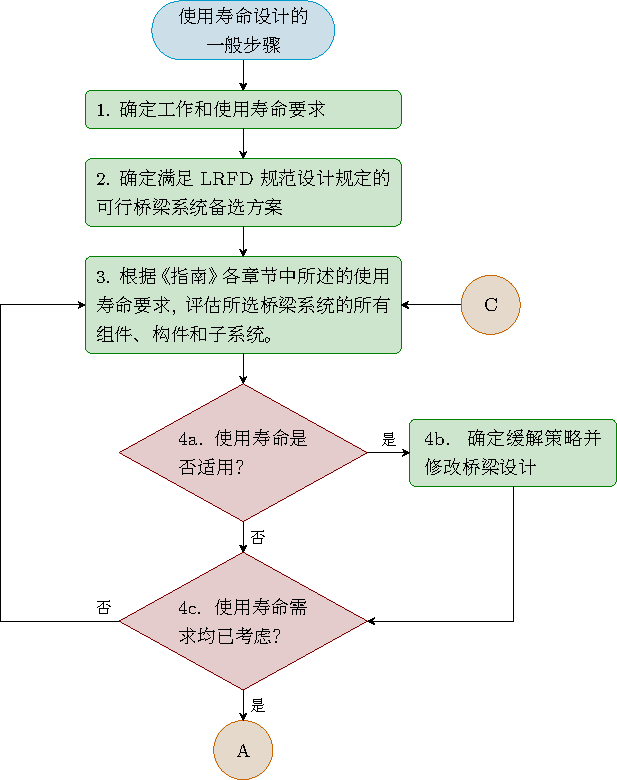
\includegraphics{flowcharta.pdf}
  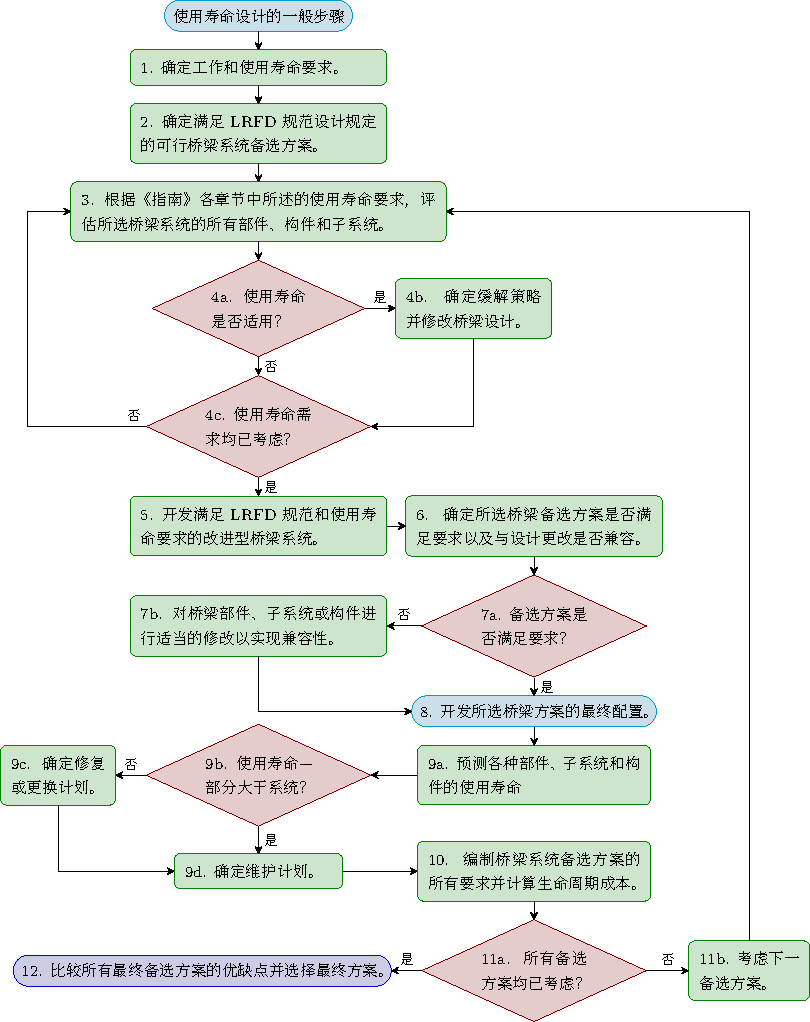
\includegraphics{flowchart.pdf}
  \caption{展示\bkn{指南}的\gls{servicelife}设计方法的总流程图}
  \label{fig:general-flowchart}
\end{figure}

  % \emph{Step 1.} The design for service life starts by first considering all project demands set by the owner, including the service life requirements, as stated in \cref{fig:general-flowchart}. \cref{chp:bridge-system-selection} provides examples of local operational and site requirements, as well as service life considerations, needing attention.
\emph{步骤 1}\quad \gls*{servicelife}设计首先考虑业主设定的所有项目需求,包括\gls{servicelife}要求,如\cref{fig:general-flowchart} 中所述。\cref{chp:bridge-system-selection}提供了本地操作和现场要求的示例,以及\gls{servicelife}注意事项,需要注意。
  
% \emph{Step 2.} Develop all feasible and preliminary bridge alternatives that satisfy project demands. For example, one might want to consider steel, concrete, and segmental bridge alternates for a particular bridge. The development of the potential bridge systems is carried out in a conventional manner, meeting all the provisions of the LRFD Specifications. It is good practice to consider potential service life problems, even at this stage of the design process. It is also feasible to use bridge technologies which do not have a specific design guideline within the LRFD Specifications. In such cases, the best available design approach could be used, subject to owner approval.
\emph{步骤 2}\quad 开发满足项目需求的所有可行和初步的桥梁备选方案。例如,人们可能想要在某特定桥梁的设计中考虑钢、混凝土和节段桥方案。潜在桥梁\gls*{system}的开发以传统方式进行,满足 \lrfd 的所有规定。优良作法是考虑潜在的\gls*{servicelife}问题,即使在设计过程的这个阶段也是如此。使用 \lrfd 中没有特定设计指南的桥梁技术也是可行的。在这种情况下,可以使用最佳可用设计方法,但须经业主批准。

  % \emph{Step 3 to 4} The next step in the process consists of evaluating each bridge system alternate one at a time and considering service life issues related to each element, component, and subsystem of that bridge system. For each bridge element, component, and subsystem, the Guide provides a framework for incorporating the changes and modifications needed to meet service life requirements.
\emph{步骤 3~4}\quad 该过程接下来的一步包括一次评估每个桥梁\gls*{system},并考虑与该桥梁\gls*{system}的每个\gls*{element}、\gls*{component}和\gls*{subsystem}相关的\gls*{servicelife}问题。对于每个桥梁\gls*{element}、\gls*{component}和\gls*{subsystem},该指南提供了一个框架,用于合并满足\gls*{servicelife}要求所需的更改和修改。

% For example, assume that one of the bridge systems to be considered for a particular project is a steel bridge alternate. The designer will first develop the preliminary bridge configurations using the conventional approaches that meet all LRFD Specifications. Then, using procedures depicted in blocks 4a, 4b, 4c, each element, component, or subsystem of the steel alternate will be checked against the service life requirements using the fault tree approach described later in the Guide. These evaluation requirements may lead to changes in the details of the element, component, or subsystem under consideration. For example, the preliminary deck configuration may indicate that use of 8-in. thick concrete is sufficient from a strength standpoint. Going through the fault tree corresponding to bridge deck and described in Chapter 4 of the Guide, the designer may change the deck thickness to 9 in. to address potential overloads, or may specify sealing the bottom of the deck to protect it from salt spray, if the bridge is located along the coastline. It should be noted that for major and complex bridges, most of these fault trees must be customized to meet specific needs and preferred practices. Examples of fault trees and how they work are provided in later sections of this chapter.
例如,假设要为特定项目考虑的桥梁\gls*{system}的备选方案之一是钢桥方案。设计人员将首先使用满足所有 \lrfd 的传统方法进行初步的桥梁设计。然后,使用模块 4a、4b、4c 中描述的程序,将使用\bkn{指南}后面描述的\gls*{faulttree}方法根据\gls*{servicelife}要求检查钢桥方案的每个\gls*{element}、\gls*{component}或\gls*{subsystem}。这些评估要求可能导致正在考虑的\gls*{element}、\gls*{component}或\gls*{subsystem}的细节发生变化。例如,从强度的角度来看,桥面板最初设计使用 \qty{20}{cm} 厚的混凝土就足够了,通过与\bkn{指南}\cref{chp:bridge-decks}中描述的桥面板对应的\gls*{faulttree},设计者可以将桥面板厚度更改为 \qty{23}{cm} 以解决潜在的超载问题,或者如果桥梁位于海岸线上,则可以指定密封桥面板底部以防止盐雾影响。应该注意的是,对于大型和复杂的桥梁,这些\gls*{faulttree}中的大多数必须定制以满足特定需求和首选实践。本章后面的部分提供了\gls*{faulttree}示例及其工作原理。

% \emph{Step 5 to 8} At the end of Step 4 and after going through appropriate fault trees for various bridge elements, components, and subsystems, the designer will have developed a bridge system that meets both strength and service life requirements, as illustrated by Step 5 in Figure 1.5. To some extent, changes to configurations of various bridge elements, components, and subsystems are carried out separately. Therefore there is a need to make sure that these changes are compatible and not contradictory or overly conservative. Steps 6 and 7 in Figure 1.5 depict this process. For example, in the steel bridge example discussed previously, service life requirements may dictate the use of a jointless, integral abutment system and require metalizing the end of the girder. The designer may then want to consider not metalizing the end of the girder, since leaking joints would be eliminated. Finally, for the selected bridge system alternate under consideration a final configuration is developed, Step 8, that meets both strength and service life requirements.
\emph{步骤 5~8}\quad 在步骤 4 结束时,在为各种\gls*{element}、\gls*{component}和\gls*{subsystem}查看适当的\gls*{faulttree}后,设计者将设计出满足强度和\gls*{servicelife}要求的桥梁\gls*{system},如\cref{fig:general-flowchart} 中的步骤 5 所示。在某种程度上,各种桥梁\gls*{element}、\gls*{component}和\gls*{subsystem}的配置更改是分开进行的。因此,需要确保这些变化是兼容的,而不是相互矛盾或过于保守的。\cref{fig:general-flowchart} 中的步骤 6 和步骤 7 描述了这个过程。例如,在前面讨论的钢桥方案的例子中,\gls*{servicelife}要求可能要求使用无缝的整体桥台系统,并且需要对大梁的末端进行金属化处理。设计师可能会考虑不对大梁的端部进行金属化处理,因为这样会消除泄漏的接头。最后,对于正在考虑中的选定桥梁\gls*{system}备选方案,将开发最终配置,即第 8 步,以满足强度和\gls*{servicelife}要求。

% \emph{Step 9 to 12} The next step in the process is to evaluate the service life of the various bridge elements, components, and subsystems of the bridge alternate under consideration and compare it to the ownerspecified target service design life of the bridge system. For example, the owner may require that the bridge provide 100 years of service life, whereas the life of a particular bridge element, such as the sliding surface for a bearing, may be limited to 20 years. There would therefore be a need to think ahead and accommodate replacement of the sliding surfaces. Regardless, there will be a need for a systematic maintenance plan that could require the designer to identify “hot areas” requiring more detailed inspection and maintenance. Blocks 9a through 9d depict the development of a maintenance plan and/or rehabilitation and replacement plan for the bridge system alternate under consideration. The result of this process, as illustrated in Step 10, is a bridge system alternate that meets both strength and service life requirements with an associated maintenance and/or rehabilitation or replacement plan for the bridge. The next step, as illustrated in Step 10, is to carry out life cycle cost analysis considering the final configuration of the select bridge alternate and maintenance plan. The same steps are repeated for all bridge alternate systems as shown by Step 11. After comparing all alternates, the designer can then make a recommendation as to which alternate should be used, allowing the owner to make the final selection.
\emph{步骤 9~12}\quad 该过程接下来的一步是评估所考虑的桥梁备选方案的各种桥梁\gls*{element}、\gls*{component}和\gls*{subsystem}的\gls*{servicelife},并将其与业主指定的桥梁\gls*{system}目标服务设计寿命进行比较。例如,业主可能要求桥梁提供 100 年的\gls*{servicelife},而特定桥梁\gls*{element}(例如支座的滑动面)的寿命可能限制为 20 年。因此,需要提前考虑并适应滑动表面的更换。无论如何,都需要一个系统的维护计划,这可能要求设计人员识别需要更详细检查和维护的“热点区域”。块 9a 到 9d 描述了正在考虑的桥梁\gls*{system}备选方案的维护计划和/或修复和更换计划的制定。如步骤 10 所示,此过程的结果是一个桥梁\gls*{system}备选方案,它满足强度和\gls*{servicelife}要求以及相关的桥梁维护和/或修复或更换计划。下一步,如第 10 步所示,是在考虑所选桥梁备选方案和维护计划的最终配置的情况下进行生命周期成本分析。如步骤 11 所示,对所有桥梁备选\gls*{system}重复相同的步骤。在比较所有备选方案后,设计人员可以就应使用哪个备选方案提出建议,让业主做出最终选择。

% As described, the selection of the final bridge system within the framework promoted in the Guide is mainly based on service life requirements. Some of the details included in the steps presented, such as fault tree analysis, will be described in later sections of this chapter.
如前所述,\bkn{指南}所提倡的框架内最终桥梁\gls*{system}的选择主要基于\gls*{servicelife}要求。所介绍的步骤中包含的一些细节,例如\gls*{faulttree}分析,将在本章后面的章节中进行描述。

% A summary of steps for design for service life is provided in \cref{sec:summary-steps} of this chapter.
本章的\cref{sec:summary-steps}中提供了\gls*{servicelife}设计步骤的总结。

% \section{Organization of the Guide}
\section{《指南》的编排组织}

% Included in the Guide are 11 chapters, each devoted to particular bridge elements, components, subsystems, or systems. The following is a brief description of information included in each chapter.
本\bkn{指南}包括 11 章,每章专门介绍特定的桥梁\gls*{element}、\gls*{component}、\gls*{subsystem}或\gls*{system}。以下是对每一章中包含的信息的简要说明。

% \cref{chp:general-frame} \nameref{chp:general-frame} This chapter provides an overview of the approach usedin the Guide for design for service life and describes terminology used throughout the Guide and various relationships that exist between service life of bridge element, component, subsystem, and system and bridge design life as used in AASHTO Specifications. The chapter provides an introduction to the different philosophies used to predict service life.
\cref{chp:general-frame} \nameref{chp:general-frame} 这一章概述了\bkn{指南}中使用的\gls*{servicelife}设计方法,并描述了指南中使用的术语以及桥梁\gls*{element}、\gls*{component}、\gls*{subsystem}和\gls*{system}的\gls*{servicelife}与 \lrfd 中使用的桥梁\gls*{designlife}之间的各种关系。这一章还介绍了用于预测\gls*{servicelife}的不同理论。

% \cref{chp:bridge-system-selection} \nameref{chp:bridge-system-selection} This chapter provides a description of various bridge systems and factors that affect their service life. Included is a description of a general strategy and rational procedure for selecting the optimum bridge system, subsystems, components, and elements, considering specific project limitations and requirements, such as climate, traffic, usage, and importance.

\cref{chp:bridge-system-selection} \nameref{chp:bridge-system-selection} 这一章描述了各种桥梁\gls*{system}以及影响其\gls*{servicelife}的因素。包括对选择最佳桥梁\gls*{system}、\gls*{subsystem}、\gls*{component}和\gls*{element}的一般策略和合理程序的描述,同时考虑特定项目的限制和要求,例如气候、交通、使用和重要性。

% \cref{chp:materials} \nameref{chp:materials} This chapter provides general properties and durability characteristics of the two most commonly used materials in bridge systems, steel and concrete. For each material, a general description of variables affecting the service life is provided, followed by strategies used to mitigate them. \cref{chp:materials} forms the basis for materials used in bridge subsystems and elements specifically addressed in other chapters of the Guide.
\cref{chp:materials} \nameref{chp:materials} 这一章介绍了桥梁\gls{system}中两种最常用的材料(钢材和混凝土)的一般特性和耐久性特征。对于每种材料,提供了影响\gls{servicelife}的变量的一般描述,然后是用于减轻这些变量影响的策略。 \cref{chp:materials} 构成了\bkn{指南}其他章节中特别提到的桥梁\gls{subsystem}和\gls{element}中所使用材料的基础。

% \cref{chp:bridge-decks} \nameref{chp:bridge-decks} This chapter provides descriptions of various bridge deck types and essential information related to their service life, such as modes of deterioration and strategies to mitigate them. The chapter concentrates on cast-in-place and precast concrete bridge decks.
\cref{chp:bridge-decks} \nameref{chp:bridge-decks} 这一章介绍了各种桥面板类型以及与其\gls{servicelife}相关的基本信息,例如\gls*{deterioration}模式和缓解策略。本章重点介绍现浇和预制混凝土桥面板。

% \cref{chp:corrosion-of-steel-rc-bridge} \nameref{chp:corrosion-of-steel-rc-bridge} This chapter looks at basic mechanisms causing corrosion of reinforcement embedded in concrete and provides strategies for preventing corrosion of reinforcement in concrete bridges.
\cref{chp:corrosion-of-steel-rc-bridge} \nameref{chp:corrosion-of-steel-rc-bridge} 这一章着眼于引起混凝土中钢筋腐蚀的基本机制,并提供防止混凝土桥梁钢筋腐蚀的策略。

% \cref{chp:corrosion-prevention-steel-bridge} \nameref{chp:corrosion-prevention-steel-bridge} This chapter provides descriptions of various coating systems using paint, galvanizing and metalizing, and descriptions of corrosion resistant steel along with factors affecting service life. Various options for preventing corrosion of steel bridges and general approaches that could lead to bridge coatings with enhanced service life are presented.
\cref{chp:corrosion-prevention-steel-bridge} \nameref{chp:corrosion-prevention-steel-bridge} 这一章介绍了油漆、镀锌和金属化的各种涂层系统,并介绍了耐腐蚀钢以及影响\gls{servicelife}的因素。介绍了防止钢桥腐蚀的各种选择以及可能导致桥梁涂层\gls{servicelife}延长的一般方法。

% \cref{chp:fatigue-fracture-steel-structures} \nameref{chp:fatigue-fracture-steel-structures} This chapter provides the basics of fatigue and fracture and factors that cause fatigue and fracture in steel bridges. Various available options for repairing observed cracking in steel bridges are also presented.
\cref{chp:fatigue-fracture-steel-structures} \nameref{chp:fatigue-fracture-steel-structures} 这一章介绍了疲劳和断裂的基础知识以及导致钢桥疲劳和断裂的因素。还介绍了修复钢桥中观察到的裂缝的各种可用方法。

% \cref{chp:jointless-bridge} \nameref{chp:jointless-bridge} This chapter provides descriptions, advantages, and disadvantages of various jointless bridge systems, and provides complete steps for design of jointless integral abutment bridges. This chapter provides design procedures to extend the application of jointless integral bridges to curved girder bridges. Also introduced are new details and integral abutment systems, where expansion joints are completely eliminated, even at the end of approach slabs.
\cref{chp:jointless-bridge} \nameref{chp:jointless-bridge} 这一章提供了各种无缝桥梁\gls{system}的描述、优点和缺点,并提供了设计无缝整体桥台桥的完整步骤。这一章提供了将无缝整体桥的应用扩展到曲线梁桥的设计程序。还引入了新的细节和在导板的末端也完全消除伸缩缝的整体式桥台\gls{system}。

% \cref{chp:expansion-devices} \nameref{chp:expansion-devices} The Guide encourages eliminating the use of expansion joints, however, expansion joints may be needed when the total bridge length exceeds practical limits of jointless bridges. This chapter describes various expansion joints used in practice, observed modes of failure for each, and potential strategies to mitigate them.
\cref{chp:expansion-devices} \nameref{chp:expansion-devices} \bkn{指南}鼓励取消使用伸缩缝,但是,当桥梁总长度超过无缝桥梁的实际限制时,可能需要使用伸缩缝。这一章描述了在实践中使用的各种伸缩缝、观察到的每种伸缩缝的故障模式,以及缓解这些故障的潜在策略。

% \cref{chp:bridge-bearings} \nameref{chp:bridge-bearings} This chapter provides descriptions of various bearing types and lists the factors that affect service life of the various bearings with strategies to mitigate them. New high performing sliding surfaces capable of providing long service life are introduced, as well as deterioration models for sliding surfaces. The Guide emphasizes use of elastomeric bearing pads.
\cref{chp:bridge-bearings} \nameref{chp:bridge-bearings} 这一章描述了各种支座类型,并列出了影响各种支座\gls{servicelife}的因素以及缓解这些因素的措施。介绍了能够提供较长\gls{servicelife}的新型高性能滑动表面,以及滑动表面的\gls*{deterioration}模型。\bkn{指南}强调使用弹性支座。

% \cref{chp:lcca} \nameref{chp:lcca} This chapter provides essential information for incorporating life cycle cost analysis (LCCA) in bridge system, subsystem, component, and element selection. It concentrates on general features and elements of incorporating LCCA in the design process, emphasizing consideration of project costs throughout its service life.
\cref{chp:lcca} \nameref{chp:lcca} 这一章提供了在桥梁\gls{system}、\gls{subsystem}、\gls{component}和\gls{element}选择中纳入\acrfull{lcca}的基本信息。它专注于将\acrlong{lcca}纳入设计过程的一般特征和要素,强调在其整个\gls{servicelife}期间考虑项目成本。


% \section{Categories of Information Provided In Guide Chapters}
\section{《指南》各章节中提供的信息类别}
% \subsubsection*{Description of Bridge Elements, Components, or Systems}
\subsubsection*{桥梁\glsentrytext{element}、\glsentrytext{component}或\glsentrytext{system}的描述}
% These sections of each chapter provide brief descriptions of, and essential information related to, both commonly used and more recently developed types of bridge components, elements, subsystems, and systems.
每章的这些部分提供了常用和最近开发的桥梁\gls{element}、\gls{component}、\gls{subsystem}和\gls{system}类型的简要描述和相关的基本信息。

% \subsubsection*{Factors that Affect Service Life}
\subsubsection*{影响\glsentrytext{servicelife}的因素}
% The factors affecting service life are identified using a fault tree approach, which provides a systematic method of identifying factors in various categories and successive subcategories. Most chapters have fault trees applicable for the types of elements, components, or subsystems covered within that chapter. In the case of major and complexbridges, designers should develop customized fault trees, reflecting the specifics associated with location and traffic conditions.
影响\gls*{servicelife}的因素是使用\gls*{faulttree}方法识别的,它提供了一种系统的方法来识别各种类别和依次子类别中的因素。大多数章节都有适用于该章所涵盖的\gls*{element}、\gls*{component}或\gls*{subsystem}类型的\gls*{faulttree}。对于大型复杂桥梁,设计人员应开发定制的\gls*{faulttree},以反映与位置和交通状况相关的具体情况。

% Following is brief description of what the fault tree is, how it is constructed, and how it works.
下面简要说明什么是\gls*{faulttree},它是如何构造的,以及它是如何工作的。

% The fault tree is used to systematically identify the factors that can affect service life of a particular bridge element, component, or subsystem. A customized fault tree can be developed using data and experiences collected from and available from local agencies.
\gls*{faulttree}用于系统地识别可能影响特定桥梁\gls*{element}、\gls*{component}或\gls*{subsystem}\gls*{servicelife}的因素。可以使用从当地机构收集的和可用的数据和经验来开发定制的\gls*{faulttree}。

% The fault tree starts with the identification of major factors that can reduce service life of a particular bridge element, component, or subsystem. Each major factor can then be broken down into more detailed subcomponents, each capable of reducing the service life. The fault tree continues branching until each branch ends with factors at the lowest or base levels of influence. The factors with subcomponents are placed inside rectangles, and the identified lowest or base factors are placed inside circles. \cref{fig:fault-tree}, for example, shows a portion of the fault tree used in Chapter 4 for bridge a deck.

\gls*{faulttree}从识别可能缩短特定桥梁\gls{element}、\gls{component}或\gls{subsystem}\gls{servicelife}的主要因素开始。然后可以将每个主要因素分解为更详细的子组件,每个子组件都会缩短\gls{servicelife}。\gls*{faulttree}继续分支,直到每个分支以最低或基本影响级别的因素结束。具有子成分的因子放置在矩形内,识别出的最低或基本因素放置在圆圈内。例如,\cref{fig:fault-tree-deck} 显示了\cref{chp:bridge-decks}中桥面系\gls*{faulttree}的一部分。

\begin{figure}
  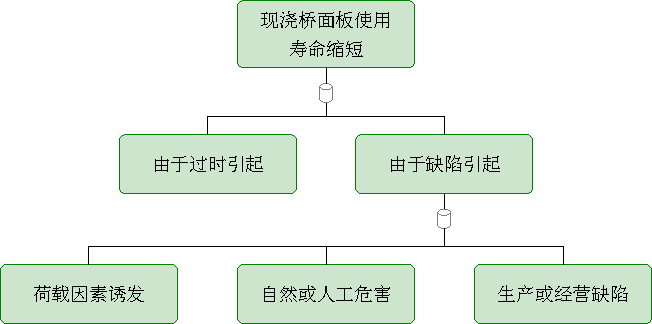
\includegraphics{fault-tree-deck.pdf}
  \caption{桥面系\gls*{faulttree}的起点}\label{fig:fault-tree-deck}
\end{figure}

% In \cref{fig:fault-tree}, either of two main factors is shown to be capable of contributing to reduced service life of a bridge deck: obsolescence or deficiency. The elliptical symbol just above these two factors is referred to as an “or gate,” which signifies that either one of the factors below it could result in reduced service life. The fault tree shown in \cref{fig:fault-tree} continues to list the major categories of factors that could result in reduced service life of bridge deck, those related to induced loads, natural or man-made hazards, and production/operation defects.

在 \cref{fig:fault-tree-deck} 中,两个主要因素中的任何一个都被证明能够导致桥面板的\gls*{servicelife}缩短:过时或缺陷。这两个因素上方的圆柱体符号称为“或门”,表示其下方的任何一个因素都可能导致\gls{servicelife}缩短。 \cref{fig:fault-tree-deck} 中显示的\gls*{faulttree}继续列出可能导致桥面板\gls{servicelife}缩短的主要因素类别,这些因素与感应载荷、自然或人为危害以及生产/运营有关缺陷。

% \cref{fig:fault-tree-deck-con}, shows the continuation of the fault tree for breakdown of factors related to load-induced factors for bridge deck.
\cref{fig:fault-tree-deck-con} 显示了\gls*{faulttree}的延续,用于分解由桥面板的负载引起的相关因素。

\begin{figure}
  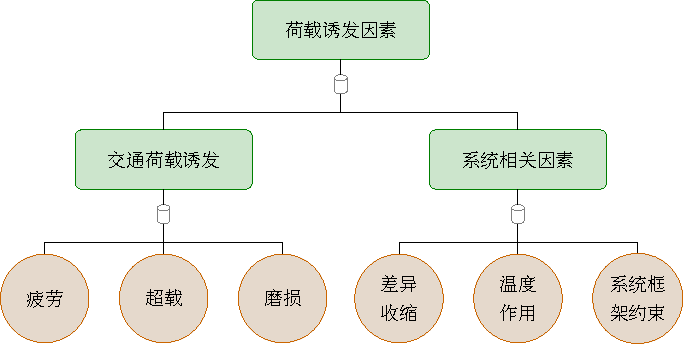
\includegraphics{fault-tree-deck-con.pdf}
  \caption{桥面系\gls*{faulttree}的延续}\label{fig:fault-tree-deck-con}
\end{figure}

% In \cref{fig:fault-tree-deck-con}, the factors related to load-induced are subcategorized into traffic-induced loads or loads induced by system-dependent loads factors, such as restraints provided by shear studs, etc. As shown in \cref{fig:fault-tree-deck-con}, two factors are further broken down into subcomponents, each capable of reducing the service life of bridge deck. The factors inside the circles are the basic factors without any further subcomponent. They represent the end of that branch of the fault tree and require the development of individual strategies to mitigate them. This aspect of process is described later.

在 \cref{fig:fault-tree-deck-con} 中,与荷载相关的因素被细分为交通引起的荷载或由系统相关荷载因素引起的荷载,例如剪力钉提供的约束等。如 \cref{fig:fault-tree-deck-con} 所示,两个因素进一步分解为子组件,每个子组件都会降低桥面板的\gls{servicelife}。圆圈内的因素是没有任何进一步子成分的基本因素。它们代表\gls*{faulttree}分支的末端,需要制定单独的策略来缓解它们。这方面的过程将在后面描述。

% In the Guide, each element of the fault tree is described immediately after introducing each branch of the fault tree. It is advisable to do the same when developing customized fault trees for major and complex bridges. Documentation of factors affecting the service life of bridge elements, components, or subsystems in the form of a fault tree, should be part of the overall plan for design for service life and provided to the owner for future reference.

在\bkn{指南}中,在介绍了\gls*{faulttree}的每个分支后,立即对\gls*{faulttree}的每个元素进行了描述。在为主要和复杂的桥梁开发定制\gls*{faulttree}时,建议这样做。以\gls*{faulttree}的形式记录影响桥梁\gls{element}、\gls{component}或\gls{subsystem}\gls{servicelife}的因素,应作为\gls{servicelife}设计总体计划的一部分,并提供给业主以供将来参考。

% \subsubsection*{Mitigation Strategies}
\subsubsection*{缓解策略}

% Where possible, each chapter provides provable solutions for major factors affecting the service life of a particular bridge element, component, subsystem, or system. Some chapters also include technology tables that summarize major characteristics associated with each solution and provide the potential solutions to factors affecting service life in a form that is easier to comprehend. For example, Figure 1.9 shows the part of the technology tables summarizing solutions for enhancing service life of bridge decks and related to traffic-induced loads as shown in \cref{fig:fault-tree-deck-con}. In \cref{fig:fault-tree-deck-con}, as part of the fault tree for bridge deck, traffic-induced loads is identified as one factor capable of reducing the service. In \cref{fig:fault-tree-deck-con}, below traffic-induced loads, three basic factors capable of reducing the service life of bridge deck are identified: Fatigue, Overload and Wear and Abrasion. Each basic factor needs to be mitigated using a select strategy, and in almost all cases, there is more than one strategy to mitigate these basic factors. It is good practice to collect these strategies in table form and select the optimal strategy, considering its interaction with other parts of bridge. The technology tables provided in various chapters of the Guide summarize strategies that can be used to mitigate various basic factors capable of reducing service life. For major and complex bridges the list of strategies could be different and based on local preferences and experiences. Most agencies have access to field data collected over the years, which could be used to construct customized strategy tables for the purpose of mitigating basic factors capable of reducing service life of bridge elements, components and subsystems.

在可能的情况下,每一章都为影响特定桥梁\gls{element}、\gls{component}、\gls{subsystem}或\gls{system}\gls{servicelife}的主要因素提供了可证明的解决方案。一些章节还包括技术表,这些表总结了与每个解决方案相关的主要特性,并以更容易理解的形式提供了影响\gls{servicelife}的因素的潜在解决方案。例如,\cref{tab:mitigating-factors-deck} 显示了技术表的一部分,总结了提高桥面板\gls{servicelife}的解决方案以及与交通引起的负载相关的解决方案,如 \cref{fig:fault-tree-deck-con} 所示。在 \cref{fig:fault-tree-deck-con} 中,作为桥面板\gls*{faulttree}的一部分,交通引起的负载被确定为能够减少服务的一个因素。在 \cref{fig:fault-tree-deck-con} 中,在交通引起的载荷下,确定了三个能够缩短桥面\gls{servicelife}的基本因素:疲劳、过载和磨损。每个基本因素都需要使用一种选择策略来减轻,并且在几乎所有情况下,都有不止一种策略来减轻这些基本因素。最好以表格形式收集这些策略并选择最佳策略,同时考虑其与桥梁其他部分的交互。本指南各章中提供的技术表总结了可用于减轻各种能够缩短\gls{servicelife}的基本因素的策略。对于主要和复杂的桥梁,策略列表可能会有所不同,并基于当地的偏好和经验。大多数机构都可以访问多年来收集的现场数据,这些数据可用于构建定制的策略表,以减轻能够降低桥梁\gls{element}、\gls{component}和\gls{subsystem}\gls{servicelife}的基本因素。

\begin{table}
  \caption{影响桥面\gls{servicelife}和与交通荷载相关的缓解因素技术表 (Table 4.3)}\label{tab:mitigating-factors-deck}
  \begin{tblr}{
  colspec={c c X[l] X[l] X[l]},
  row{1}={c,bg=genfg,fg=white,font=\bfseries,guard}
}
\SetCell[c=2]{m,c}\glsentrytext{servicelife}问题 & & 缓解策略 & 优点 & 缺点 \\
\SetCell[r=4]{m,c,bg=genbgd!50}{交通\\荷载\\问题} 
& 疲劳                   & 按 \acrshort{lrfd} 规范设计        & 最大限度地减少钢筋失效的可​​能性 & 可能会增加钢材的用量 \\
& 超载                   & 增大桥面板厚度                     & 最大限度地减少开裂             & 增加桥梁结构的重量,增加造价成本 \\
& \SetCell[r=2]{m,c,bg=genbgd!20}磨损 & 调整混凝土配合比设计               & 见 \cref{chp:materials} \nameref{chp:materials} & 见 \cref{chp:materials} \nameref{chp:materials} \\
&                        & 加设薄膜与覆盖层                   & 保护表面不与轮胎直接接触       & 需要每 10 到 20 年进行一次定期维护 \\
\end{tblr}
\end{table}

% The sample table in \cref{tab:mitigating-factors-deck} lists the advantages and disadvantages for each possible solution capable of mitigating the adverse service life consequences of traffic-induced loads. In some cases, more information than just advantages and disadvantages are provided, such as qualitative assessment of maintenance cost. For major and complex bridges additional considerations may be included in technology tables.

\cref{tab:mitigating-factors-deck} 列出了每种可能的解决方案的优缺点,这些解决方案能够减轻交通引起的负载对\gls{servicelife}的不利影响。在某些情况下,提供的信息不仅仅是优点和缺点,例如维护成本的定性评估。对于主要和复杂的桥梁,技术表中可能包含其他考虑因素。

% \subsubsection*{Optimum Selection Strategies}
\subsubsection*{最佳选择策略}
% Overall strategies are provided for achieving enhanced service life. The overall strategy approach provided depends on the particular bridge component, element, subsystem, or system. \cref{fig:overall-strategy} shows an example of the overall strategy for selecting a bearing that meets both strength and service life requirements, taken from \cref{chp:bridge-bearings} of the Guide.

提供的实现延长\gls*{servicelife}的总体策略方法取决于特定的桥梁\gls*{element}、\gls*{component}、\gls*{subsystem}或\gls*{system}。\cref{fig:overall-strategy-bearing} 显示了选择同时满足强度和\gls*{servicelife}要求的支座的总体策略示例,摘自\bkn{指南}的\cref{chp:bridge-bearings}。

\begin{figure}
  % \includegraphics{overall-strategy-bearing.pdf}
  \caption{考虑\gls{servicelife}的支座设计总体策略}\label{fig:overall-strategy-bearing}
\end{figure}

% It should be noted that the chapter devoted to bearings, \cref{chp:bridge-bearings}, identifies factors affecting service life of bearings and provides potential solutions for each. This information, combined with steps outlined in the flowchart, can be used as a rational approach for selecting an appropriate bearing that meets project requirements with emphasis on service life.

应该注意的是,专门介绍支座的章节\cref{chp:bridge-bearings}确定了影响支座\gls{servicelife}的因素,并为每个因素提供了可能的解决方案。此信息与流程图中概述的步骤相结合,可用作选择满足项目要求并强调\gls{servicelife}的合适支座的合理方法。


% \subsubsection*{Examples and Tools}
\subsubsection*{示例与工具}
% Most chapters include examples demonstrating the application of strategies in that chapter.

大多数章节都包含示例以展示该章中策略的应用。

% \section{Quantifying Service Life of Bridge Element, Component, Subsystem, and System}
\section{桥梁\glsentrytext{element}、\glsentrytext{component}、\glsentrytext{subsystem}和\glsentrytext{system}\glsentrytext{servicelife}的量化}

% One of the important steps in developing a systematic, comprehensive service life design plan for bridges is the capability to predict the expected service life of various bridge elements, components, and subsystems, which in turn will dictate the service life of the bridge system. This is Step 9a shown in Figure 1.6. The service life prediction capability is important for developing maintenance, retrofit, and replacement plans, which are an integral part of service life design process. The objective of this section is to provide an overview of the methodology used in the Guide for predicting the service life.
制定系统的、全面的桥梁\gls*{servicelife}设计计划的重要步骤之一是预测各种桥梁\gls*{element}、\gls*{component}和\gls*{subsystem}的预期\gls*{servicelife}的能力,这反过来将决定桥梁系统的\gls*{servicelife}。 这是\cref{fig:general-flowchart}中所示的步骤 9a。 \gls*{servicelife}预测能力对于制定维护、改造和更换计划非常重要,这些都是\gls*{servicelife}设计过程中不可或缺的一部分。 本节的目的是概述\bkn{指南}中用于预测\gls*{servicelife}的方法。

% Bridge elements, components, subsystems, and systems are subject to the effects of traffic and the environment. These external sources of deterioration act through various mechanisms to cause actual deterioration of bridge elements and eventually failure. The mechanisms of deterioration are the physical laws that govern such deterioration. Deterioration rates can be described using mathematical expressions or empirical/semiempirical models, which are developed using data collected by field monitoring of bridges, laboratory generated data, expert opinions, or combination of available data. Service life is also affected by risk to damage either from traffic or extreme environmental occurrences. The acceptability of this damage is evaluated based on risk. Service life can be extended by minimizing risk or designing for appropriate levels of extreme occurrences.
桥梁\gls*{element}、\gls*{component}、\gls*{subsystem}和\gls*{system}会受到交通和环境的影响。 这些外部\gls*{deterioration}源通过各种机制起作用,导致桥梁\gls{element}实际\gls*{deterioration}并最终失效。 \gls*{deterioration}机制是支配这种\gls*{deterioration}的物理定律。 可以使用数学表达式或经验/半经验模型来描述\gls*{deterioration}率,这些模型是使用桥梁现场监测收集的数据、实验室生成的数据、专家意见或可用数据的组合开发的。 \gls*{servicelife}还受到交通或极端环境事件造成的损坏风险的影响。 这种损害的可接受性是根据风险来评估的。 通过最大限度地降低风险或针对极端事件的适当级别进行设计,可以延长\gls*{servicelife}。

% Enhanced service life for bridge elements, components, subsystems, and systems can be achieved through:
可以通过以下方式延长桥梁\gls*{element}、\gls*{component}、\gls*{subsystem}和\gls*{system}的\gls*{servicelife}:

\begin{itemize}
  % \item Use of durable materials,
  \item 使用耐久性材料;
  % \item Use of either passive or active protection systems,
  \item 使用主动或被动的保护系统;
  % \item Optimum selection of details,
  \item 采用最佳细部构造;
  % \item Optimum maintenance and repair,
  \item 采用最佳的运营维护和维修;
  % \item Reduced service level,
  \item 降低服务水平;
  % \item Increased factor of safety or reduction in stress levels, and
  \item 增加安全系数或降低应力水平;
  % \item Isolation from risk damage.
  \item 隔离风险损害。
\end{itemize}

% To estimate the service life of bridge elements, components, or subsystems quantitatively, the following information is needed:
要定量估算桥梁\gls*{element}、\gls*{component}或\gls*{subsystem}的\gls*{servicelife},需要以下信息:
\begin{itemize}
  % \item Source of deterioration,
  \item \gls*{deterioration}产生的根源;
  % \item Deterioration mechanism,
  \item \gls*{deterioration}机制;
  % \item Deterioration models, and
  \item \gls*{deterioration}模型;
  % \item Failure modes.
  \item 失效模式。
\end{itemize}

% The following sections provide information on each of these items.
以下部分提供了有关其中每一项的信息。

\subsubsection*{\gls*{deterioration}产生的根源}
% Traffic related or environmental effects form the basic external cause of deterioration. For example, deicing compounds, an external source of deterioration, can result in corrosion of reinforcement in bridge elements
交通相关或环境影响构成\gls*{deterioration}的基本外部原因。例如,除冰化合物是\gls*{deterioration}的外部来源,会导致桥梁\gls{element}中钢筋的腐蚀。

\subsubsection*{\gls*{deterioration}机制}
% Deterioration is governed by a process called the deterioration mechanism. For example, sliding surfaces in bearings experience deterioration through horizontal movement and friction between sliding materials, created by truck passages or temperature fluctuations. The horizontal movement and friction in this instance is the deterioration mechanism. In the case of concrete elements, ingress of chloride through concrete causes initiation of corrosion in unprotected steel reinforcement. In this instance, the ingress of chloride is the deterioration mechanism.
控制\gls*{deterioration}的过程的机理称之为\gls*{deterioration}机制。例如,支座的滑动表面会因卡车通行或温度波动造成的水平运动和滑动材料之间的摩擦而\gls*{deterioration}。 这种情况下的水平运动和摩擦是\gls*{deterioration}机制。 对于混凝土构件,氯离子渗透通过混凝土会导致未受保护的钢筋发生腐蚀。 在这种情况下,氯离子的渗透是\gls*{deterioration}机制。

\subsubsection*{\gls*{deterioration}模型}
% Deterioration models are used to describe the rate of deterioration. They describe the relationship between the condition of the bridge (or its element) and its time of use, and show how the bridge deteriorates over time. It assumes that no replacements or major repairs are made, but it usually implies that scheduled maintenance actions are performed as planned. The basic model applies either to a bridge system as a whole, or to any of its subsystems, components or elements.
\gls*{deterioration}模型用于描述\gls*{deterioration}率。 它们描述了桥梁(或其\gls*{element})的状况与其使用时间之间的关系,并显示了桥梁如何随着时间的推移而\gls*{deterioration}。 它假设没有进行任何更换或大修,但通常意味着按计划执行了定期维护操作。 基本模型既适用于整个桥梁\gls*{system},也适用于其任何\gls*{subsystem}、\gls*{component}或\gls*{element}。

% An example of a deterioration curve is presented in \cref{fig:bridge-deterioration-curve}. If the bridge is placed in service at period T0, its condition gradually declines, and the deterioration curve represents its condition over time. Initially the condition is good, but after a period of wear and aging, it eventually (at time Tf) reaches an unacceptably low condition Cf. The time period between T0 and Tf is called Service Life (SL) of the bridge.
\cref{fig:bridge-deterioration-curve} 中给出了\gls*{deterioration}曲线的一个例子。 如果桥梁在 $T_0$ 期间投入使用,其状况会逐渐下降,\gls*{deterioration}曲线表示其随时间变化的状况。最初状况良好,但经过一段时间的磨损和老化后,最终(在时间 $T_\text{f}$)达到无法接受的低状况 $C_\text{f}$。 $T_0$ 和 $T_\text{f}$ 之间的时间段称为桥梁的\acrfull{sl}。

\begin{figure}
  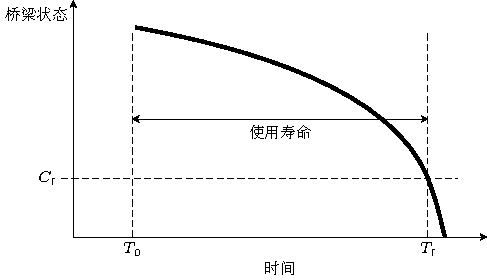
\includegraphics{bridge-deterioration-curve.pdf}
  \caption{桥梁\gls*{deterioration}曲线示例}\label{fig:bridge-deterioration-curve}
\end{figure}

% In practice, the development of realistic behavioral deterioration models is a data-intensive process complicated by lack of knowledge of the underlying physical and chemical processes fostering deterioration, as well as by the data availability. At the present time the available deterioration models, which are based on long-term data collection, are very limited. Further, as time passes, the quality of the bridge design and construction improves. As a result, application of data collected from existing bridges to predict performance of future bridges should be practiced with caution.
在实践中,现实行为\gls*{deterioration}模型的开发是一个数据密集型过程,由于缺乏对促进\gls*{deterioration}的潜在物理化学过程的知识以及数据可用性而变得复杂。目前,基于长期数据收集的可用\gls*{deterioration}模型非常有限。此外,随着时间的推移,桥梁设计和施工的质量也会提高。因此,应谨慎应用从现有桥梁收集的数据来预测未来桥梁的性能。

% Deterioration models capable of quantitatively predicting the service life of bridge elements, components, subsystems, or systems are very limited or nonexistent. The most acceptable deterioration model is in the form of the solution to Fick's second law, used to predict the rate of chloride ingress through concrete cover. This model, including its limitations, is described in \cref{chp:corrosion-of-steel-rc-bridge} of the Guide. It is expected that with time, more deterioration models will become available and will greatly enhance quantification of the service life of bridge elements, components, subsystems, or systems.
能够定量预测桥梁\gls*{element}、\gls*{component}、\gls*{subsystem}或\gls*{system}\gls*{servicelife}的\gls*{deterioration}模型非常有限或不存在。最可接受的\gls*{deterioration}模型采用菲克第二定律的解形式,用于预测氯离子通过混凝土保护层的侵入率。该模型及其局限性在\bkn{指南}的 \cref{chp:corrosion-of-steel-rc-bridge} 中进行了描述。预计随着时间的推移,将有更多的\gls*{deterioration}模型可用,并将大大提高桥梁\gls*{element}、\gls*{component}、\gls*{subsystem}或\gls*{system}\gls*{servicelife}的量化。

% As shown on \cref{fig:condition-life-cycle}, if left alone a bridge will deteriorate over the period of its service life. However, in most cases a bridge is not left to follow the basic deterioration path and reach an unacceptable condition without interruption. The agency responsible for the bridge will from time to time undertake repairs, rehabilitations, and renewals that return conditions to higher levels and extend its service life. During these interventions, the condition rate of the bridge condition increases, as depicted in \cref{fig:condition-life-cycle}.
如\cref{fig:condition-life-cycle} 所示,如果任其发展,桥梁状况将在其\gls*{servicelife}期间\gls*{deterioration}。然而,在大多数情况下,桥梁不会沿着基本的\gls*{deterioration}路径发展并在不中断的情况下达到不可接受的状态。桥梁主管机构将不时进行维修、修复和更新,使桥梁状况恢复到更高水平并延长其\gls*{servicelife}。在这些干预期间,桥梁状况的状况率增加,如\cref{fig:condition-life-cycle} 中所示。

\begin{figure}
  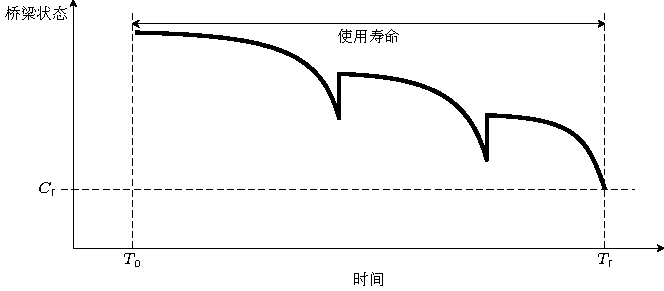
\includegraphics{condition-life-cycle.pdf}
  \caption{桥梁在整个生命周期内状况}\label{fig:condition-life-cycle}
\end{figure}

% Deterioration models can also be based on some level of understanding of the mechanism governing the deterioration and the capability to express the process using a mathematical expression. An example is deterioration of concrete elements because of chloride induced corrosion of reinforcement. The assumption is that ingress of chloride through the concrete element is governed by Fick's second law, which assumes a homogeneous material.

\gls*{deterioration}模型可以基于对控制\gls*{deterioration}机制的某种程度的理解以及运用数学表达式表达其过程的能力。一个例子是由于氯离子引起的钢筋腐蚀而导致混凝土构件\gls*{deterioration}。这其中,我们假定混凝土材料是均质的,氯离子在混凝土中的渗透符合菲克第二定律。

% In the case of chloride and carbonation induced corrosion, there is some level of agreement within the scientific community as to the existence of deterioration models. However, for other deterioration modes such as sulfate attack, alkali-silica reactivity (ASR), and freeze/thaw or wear and abrasion, there is a lack of adequate models. Further, as described earlier, the use of deterioration models to predict the time to initiate corrosion of reinforcement embedded within certain distances of the concrete surface because of chloride ingress, should be approached with caution. Following is brief description of a deterioration model for chloride induced corrosion.

在氯离子和碳化引起的腐蚀的情况下,科学界对\gls*{deterioration}模型存在一定程度的共识。然而,对于其他\gls*{deterioration}模式,如硫酸盐侵蚀、\acrlong{asr}(\acrshort{asr})、冻融或磨损,缺乏足够的模型。此外,如前所述,使用\gls*{deterioration}模型来预测由于氯离子渗透混凝土表面一定距离内的钢筋开始腐蚀的时间,应谨慎处理。以下是氯离子引起的腐蚀的\gls*{deterioration}模型的简要描述。

% There are different approaches to solving Fick's second law. A finite difference approach, or the use of error functions, is reported in published literatures. Equation 1.4 is an error function solution of Fick's second law, capable of predicting the chloride concentration level at various depths within the concrete element.

求解菲克第二定律有不同的方法。已发表的文献采用了有限差分法或误差函数解法。\cref{eq:ficks-second-law} 是菲克第二定律的误差函数解,能够预测混凝土构件内不同深度的氯离子浓度水平。
\begin{equation}
  \label{eq:ficks-second-law}
  C_\text{crit} = C(x=a, t) = C_0 +(C_{\text{S},\Delta x} - C_0)\left[ 1-\erf 
   \frac{a-\Delta x}{2\sqrt{D_{\text{app},\text{C}}\cdot t}} \right]
\end{equation}
\begin{EqDesc}{C(x,t)}
  \item[C_\text{crit}] 临界氯离子含量(重量百分比 \%);
  \item[C(x,t)] 在深度 $x$(结构表面:$x=\qty{0}{mm}$)处和时间 $t$ 时混凝土中氯离子的含量(重量百分比 \%);
  \item[C_0] 混凝土初始氯离子含量(重量百分比 \%);
  \item[C_{\text{S},\Delta x}] 深度 $\Delta x$ 处和某个时间点 $t$ 的氯离子含量(重量百分比 \%);
  \item[x] 对应氯离子含量 $C(x,t)$ 的深度(\unit{mm});
  \item[a] 混凝土保护层(\unit{mm});
  \item[\Delta x]对流区(混凝土中氯离子渗透过程不同于菲克第二扩散定律的部分)深度(\unit{mm});
  \item[D_{\text{app},\text{C}}] 氯离子在混凝土中的表观扩散系数(\unit{mm^2/yr});
  \item[t] 时间(\unit{yr});
  \item[\erf] 误差函数。
\end{EqDesc}

% \cref{eq:ficks-second-law} should be used in conjunction with probabilistic approaches to account for variability of several parameters, such as apparent coefficient of diffusion, chloride concentration, and critical chloride level to start corrosion. Furthermore, the diffusivity of concrete through different layers of concrete element is not uniform. \cref{eq:ficks-second-law} predicts the chloride content in the structure at a given depth (x) and time (t). This number is given by the left-hand side of the equation, C(x,t).

\cref{eq:ficks-second-law} 应与概率方法结合使用,以解释多个参数的可变性,例如表观扩散系数、氯离子浓度和开始腐蚀的临界氯离子水平。此外,混凝土通过不同层的混凝土的扩散率是不均匀的。 \cref{eq:ficks-second-law} 预测给定深度($x$)和时间($t$)下结构中的氯离子含量。该数字由等式的左侧 $C(x,t)$ 给出。

% The C(x,t) obtained from \cref{eq:ficks-second-law} is then compared to the critical chloride content, Ccrit , which is the value determined to be the point at which corrosion starts. When the chloride level at a given depth, x, of the structure is reached, the critical value, the corrosion is assumed to initiate. The service life of concrete element can then be assumed to consist of the time period to initiate corrosion plus the time period for propagation of the corrosion to the point that will limit the functionality of concrete element. This process is depicted in \cref{fig:damage-service-life}.

将从\cref{eq:ficks-second-law} 获得的 $C(x,t)$ 与临界氯离子含量 $C_\text{crit}$ 进行比较,该值被确定为腐蚀开始点。当结构的给定深度 $x$ 处的氯离子水平达到临界值时,我们认为腐蚀开始。然后可以假定混凝土的\gls*{servicelife}包括开始腐蚀的时间段加上腐蚀传播到将限制混凝土功能的点的时间段。这个过程在\cref{fig:damage-service-life} 中描述。

\begin{figure}
  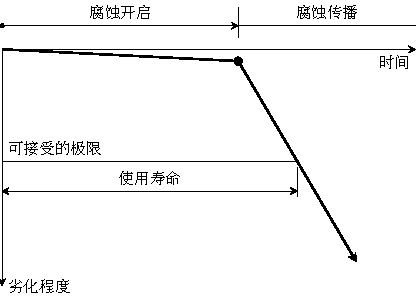
\includegraphics{damage-service-life.pdf}
  % \caption{Relationship between damage and service life. (Source COWI, Denmark)}
  \caption{损伤与\gls*{servicelife}的关系}
  \label{fig:damage-service-life}
\end{figure}

\subsubsection*{失效模式}
% Sources of deterioration (such as deicing compounds), acting through deterioration mechanisms (such as ingress of chloride through concrete cover), and described by deterioration models (such as solution to Fick's second law) result in failure modes (corrosion of reinforcement, causing corrosion induced cracking and loss of strength). The final failure could consist of several stages, such as start and propagation phases.
\gls*{deterioration}源(例如除冰盐等化合物)通过\gls*{deterioration}机制(例如氯离子渗透通过混凝土保护层)起作用,并由\gls*{deterioration}模型(如菲克第二定律的解)描述导致失效模式(钢筋腐蚀,导致腐蚀引起开裂和强度损失)。最终故障可能包括几个阶段,例如开始阶段和传播阶段。

\subsubsection*{\glsentrytext{servicelife}评估}
% In the Guide, two general philosophies are presented to estimate the service life of bridge elements, components, and subsystems. The end result of quantifying the service life of bridge elements, components, or subsystems is to establish the ts, the service life of bridge elements, components, or subsystems, and compare it to specified service life of the bridge system to determine the need for retrofit or replacement strategies if needed.
\bkn{指南}提出了两种一般性原理来估算桥梁\gls*{element}、\gls*{component}和\gls*{subsystem}的\gls*{servicelife}。量化桥梁\gls*{element}、\gls*{component}或\gls*{subsystem}\gls*{servicelife}的最终结果是建立桥梁\gls*{element}、\gls*{component}或\gls*{subsystem}的\gls*{servicelife} $t_\text{s}$,并将其与桥梁\gls*{system}的指定\gls*{servicelife}进行比较以确定是否需要改造或更换策略。

% Two general design approaches for service life are:
两种通用的\gls*{servicelife}设计方法是:
\begin{itemize}
  \item 有限\gls*{servicelife}法;
  \item 目标\gls*{servicelife}法。
\end{itemize}

% When the design service life, ts, of the bridge element, component, or subsystem, established through one of the two design approaches for service life philosophies is less than the specified design life of the bridge system, tD, the bridge element, component, or subsystem under consideration could be replaced to achieve the specified design life of the bridge system.
当通过两种\gls*{servicelife}理念设计方法之一确定的桥梁\gls*{element}、\gls*{component}或\gls*{subsystem}的设计\gls*{servicelife} $t_\text{s}$ 小于桥梁\gls*{system}的指定\gls*{designlife} $t_\text{D}$ 时,桥梁\gls*{element}、\gls*{component}、 或正在考虑的\gls*{subsystem}可以更换,以达到桥梁\gls*{system}的指定\gls*{designlife}。

% The major difference between the two approaches for service life design is the existence of well-accepted deterioration models, which is needed before using the finite service life approach.
两种\gls*{servicelife}设计方法的主要区别在于存在广为接受的\gls*{deterioration}模型,这是在使用有限\gls*{servicelife}方法之前所必需的。

\paragraph*{有限\gls*{servicelife}法}
% Bridge elements, components, and subsystems designed using the finite service life approach, should have service life that is greater than or equal to specified bridge system service life. Otherwise, the bridge element, component, or subsystem under consideration must be retrofitted or replaced to allow the bridge to continue providing its intended function until reaching the specified bridge system service life. In the finite service life approach, the service life of the bridge components, elements, or subsystems is estimated using well-accepted deterioration models. The existence of deterioration models is therefore essential for use of the finite service life approach.
使用有限\gls*{servicelife}方法设计的桥梁\gls*{element}、\gls*{component}和子系统的\gls*{servicelife}应大于或等于指定的桥梁\gls*{system}\gls*{servicelife}。 否则,必须对所考虑的桥梁\gls*{element}、\gls*{component}或\gls*{subsystem}进行改造或更换,以使桥梁继续提供其预期功能,直至达到规定的桥梁\gls*{system}\gls*{servicelife}。 在有限\gls*{servicelife}法中,桥梁\gls*{component}、\gls*{element}或\gls*{subsystem}的\gls*{servicelife}使用广为接受的\gls*{deterioration}模型进行估算。 因此,\gls*{deterioration}模型的存在对于使用有限\gls*{servicelife}方法是必不可少的。

% The deterioration models are generally developed using one of the following approaches:
\gls*{deterioration}模型通常使用以下方法之一开发:
% \begin{itemize}
%   \item Mathematical models which describe the deterioration rate. These models could be approximate or based on laws of physics.
%   \item Empirical or semiempirical models developed using data collected from laboratory or field performance of bridges. Fatigue models used in the LRFD Specifications is an example of empirical deterioration model.
%   \item Empirical models based on expert opinions or experiences. Examples include various models used in \pontis.
% \end{itemize}
\begin{itemize}
  \item 描述\gls*{deterioration}率的数学模型。这些模型可以基于物理定律或是近似的。
  \item 使用从实验室或桥梁现场性能收集的数据开发的经验或半经验模型。 例如 \lrfd 中使用的疲劳模型即是一个经验\gls*{deterioration}模型。
  \item 基于专家意见或经验的经验模型。 例如 \pontis 中使用的各种模型。
\end{itemize}

% Where deterioration models exist, the service life design could be in the form of:
在存在\gls*{deterioration}模型的情况下,使用寿命设计可以采用以下形式:

% \emph{Full probabilistic approach}. This approach requires having probability distribution functions for all variables used in the deterioration model.
\emph{全概率方法}。这种方法需要为恶化模型中使用的所有变量提供概率分布函数。

% \emph{Semiprobabilistic or partial load factor approach}. This approach is developed using full probabilistic approach. It is equivalent to using load and resistance factors in the LRFD Specifications versus using full probabilistic approach (such as using Mont Carlo simulation) to design or rate bridges.
\emph{半概率或部分荷载系数方法}。 这种方法是使用全概率方法开发的。 它相当于使用 \lrfd 中的荷载—抗力系数与使用完全概率方法(例如使用蒙特卡洛模拟)来设计或评估桥梁。

\paragraph*{目标\gls*{servicelife}法}
% In many instances the deterioration models are not available or their applicability is questionable. In these situations, available alternatives are 
在许多情况下,\gls*{deterioration}模型不可用或它们的适用性值得怀疑。在这些情况下,可用的替代方案是
\begin{enumerate*}
  % \item  use of high performing material that does not deteriorate, such as use of stainless steel, an approach is generally referred to as the avoidance of deterioration method within European practice, or 
  \item 使用不会\gls*{deterioration}的高性能材料,例如使用不锈钢,这种方法在欧洲实践中通常被称为避免\gls*{deterioration}方法;
  % \item use material that based on experience, or based on expert opinion, could provide a specified or a target service life. If the estimated service life of the bridge element, component, or subsystem is less than the specified service life of the bridge, retrofit or replacement strategies must be specified, allowing the bridge system to continue providing its intended function.
  \item 使用基于经验或专家意见的材料,可以提供指定或目标\gls*{servicelife}。如果桥梁\gls*{element}、\gls*{component}或\gls*{subsystem}的估计\gls*{servicelife}小于桥梁的指定\gls*{servicelife},则必须指定改造或更换策略,使桥梁\gls*{system}继续提供其预期功能。
\end{enumerate*}

% The major difference between finite service life and target service life design approaches is that in finite service life design approach, the condition of the bridge element, component, and subsystem can be traced over time using deterioration models, whereas in target service life design approach, only the total expected service life is estimated. The specified target service life of bridge element, component, or subsystem is mainly established based on experience or expert opinion, and could vary significantly from assumed values. Nevertheless, specifying a target service life for a given bridge element, component, or subsystem allows the bridge owner to plan and anticipate necessary maintenance actions and places demands on the designer to incorporate necessary design features where needed. For example, the service life of PTFE sliding surfaces in bearing devices could be assumed to be about ten years (target service life of 10 years). The designer must then incorporate necessary mechanisms to lift the bridge and replace the sliding surfaces, preferably while maintaining traffic. On the other hand, the bridge owner must plan and anticipate the replacement of sliding surfaces every 10 years.
有限\gls*{servicelife}法和目标\gls*{servicelife}法之间的主要区别在于,在有限\gls*{servicelife}法中,可以使用\gls*{deterioration}模型跟踪桥梁\gls*{element}、\gls*{component}和\gls*{subsystem}随时间推移的状况,而在目标\gls*{servicelife}设计方法中,仅估算总预期\gls*{servicelife}。桥梁\gls*{element}、\gls*{component}或\gls*{subsystem}的指定目标\gls*{servicelife}主要是根据经验或专家意见确定的,可能与假定值有很大差异。然而,为给定的桥梁\gls*{element}、\gls*{component}或\gls*{subsystem}指定目标\gls*{servicelife}允许桥梁所有者计划和预测必要的维护行动,并要求设计师在需要时纳入必要的设计特征。例如,支座装置中 \acrlong{ptfe} 滑动表面的\gls*{servicelife}可以假设为大约 10 年(目标\gls*{servicelife}为 10 年)。然后,设计师必须结合必要的机制来提升桥梁并更换滑动表面,最好是在维持交通的同时。另一方面,桥梁所有者必须计划和预期每 10 年更换一次滑动面。

% \section{Owner's Manual}
\section{使用手册}

% In instances where specified by the owner and for major and complex bridges, the final step in the design for service life process is the development of a bridge Owner's Manual, which summarizes the processes used for design for service life and provides complete descriptions of outcomes and recommendations. The intention is to equip the owner with the necessary knowledge to keep the bridge operational for the specified service life period. The bridge Owner's Manual should be provided to the owner at the time of opening the bridge to traffic, following an independent review process described in the next section.

在业主指定的情况下,对于主要的和复杂的桥梁,\gls{servicelife}设计流程的最后一步是制定桥梁使用手册,该手册总结了\gls{servicelife}设计所使用的流程,并提供了对结果的完整描述和建议。目的是让业主掌握必要的知识,使桥梁在指定的\gls{servicelife}期间保持正常运行。桥梁使用手册应在桥梁通车时提供给业主,并遵循下一节所述的独立审查程序。

% The entire process used for design for service life should be well documented and include assumptions, limitations, and any other information of which the owner should be aware, including complete information with respect to “hot spots” within various bridge elements, components, or subsystems that will require closer inspection, maintenance, retrofit, or replacement. The Owner's Manual should include a complete management plan with respect to service life, including information on timely maintenance actions, and identify replacement items and methodologies for replacement with information on the required level of traffic interruption, if any. In the case of major and complex bridges it is suggested that a bridge instrumentation and monitoring plan be developed and be tied to the bridge service life management plan. Additional information to be included in the Owner's Manual after construction should include the actual material properties of critical bridge elements versus the assumed values used in the design process. Such information is important for future bridge rating.

用于\gls{servicelife}设计的整个过程应妥善记录,这其中包括假定、限制和所有者应了解的任何其他信息,如需要更仔细的检查、维护、改造或更换的有关各种桥梁\gls{element}、\gls{component}或\gls{subsystem}中“热点”的完整信息。用户手册应包括有关\gls{servicelife}的完整管理计划,包括有关及时维护措施的信息,确定更换项目和更换方法以及所需交通中断级别的信息(如果有)。对于大型和复杂的桥梁,建议制定桥梁检测和监测计划,并将其与桥梁\gls{servicelife}管理计划联系起来。施工后要包含在用户手册中的其他信息应包括关键桥梁\gls{element}的实际材料特性与设计过程中使用的假定值的对比。这些信息对未来的桥梁评级很重要。

% With respect to major and complex bridges, the designer should use sound engineering judgment for determining the level and extent of information to be included in the Owner's Manual. The bridge Owner's Manual is analogous to the design calculations that are customarily provided to the bridge owner, except that the Owner's Manual contains much more detailed information.

对于主要和复杂的桥梁,设计者应使用合理的工程判断来确定要包含在用户手册中的信息的级别和范围。桥梁所有者手册类似于通常提供给业主的设计计算,只是所有者手册包含更多详细信息。

% \section{Independent Review of Design for Service Life Process}
\section{\glsentrytext{servicelife}设计过程的独立审查}

% The design for service life processes, results, and recommendations as summarized in the bridge Owner's Manual, should be checked by an independent and knowledgeable third party. This independent check is analogous to an independent design check typically conducted for bridge design.

桥梁用户手册中总结的\gls{servicelife}设计的过程、结果和建议应由独立且有经验的第三方进行检查。这种独立检查类似于通常针对桥梁设计进行的独立设计检查。

% \section{Summary of Steps for Design for Service Life for Specific Bridge Element, Component, and Subsystem}\label{sec:summary-steps}
\section{特定桥梁\glsentrytext{element}、\glsentrytext{component}和\glsentrytext{system}的\glsentrytext{servicelife}设计步骤总结}\label{sec:summary-steps}

% This section provides a summary of the steps in design for service life. Detailed description of individual steps is provided in \cref{sec:guide-approach}.

本节总结了\gls{servicelife}设计的步骤。 \cref{sec:guide-approach} 中提供了各个步骤的详细说明。

% Bridge elements, components, and subsystems can deteriorate at different rates and have different service lives. This governs the service life of a bridge system, which is reached when the service life of critical bridge elements, components, or subsystems is exhausted beyond being repaired or replaced economically or because of other considerations.

桥梁\gls{element}、\gls{component}和\gls{subsystem}可能会以不同的速度\gls*{deterioration}并具有不同的\gls{servicelife}。这决定了桥梁\gls{system}的\gls{servicelife},当关键桥梁\gls{element}、\gls{component}或\gls{subsystem}的\gls{servicelife}耗尽而无法经济地修复或更换或出于其他考虑时,就会达到桥梁\gls{system}的\gls{servicelife}。

% The general steps in design for service life for particular a bridge element, component or subsystem can be summarized are as follows:
特定桥梁\gls{element}、\gls{component}或\gls{subsystem}的\gls{servicelife}设计的一般步骤可概括如下:

\begin{description}[style=nextline,leftmargin=6.5em]
  % \item [步骤 1] Identify the project requirements, particularly those that will influence the service life.
  \item [步骤 1] 确定项目要求,尤其是那些会影响\gls{servicelife}的要求。
  % \item [步骤 2] Identify feasible bridge systems capable of meeting the project demand.
  \item [步骤 2] 确定能够满足项目需求的可行桥梁\gls{system}。
  % \item [步骤 3] Select each feasible bridge system one at a time and complete Steps 4 through 10.
  \item [步骤 3] 一次选择每个可行的桥梁\gls{system}并完成步骤 4 到 10。
  % \item [步骤 4] Identify the factors that influence the service life of bridge elements, components, and subsystems, such as traffic and environmental factors.
  \item [步骤 4] 确定影响桥梁\gls{element}、\gls{component}和\gls{subsystem}\gls{servicelife}的因素,例如交通和环境因素。
  % \item [步骤 5] Identify modes of failures and consequences. For instance, the corrosion of reinforcement causing corrosion induced cracking and loss of strength.
  \item [步骤 5] 确定故障模式和后果。例如,钢筋的腐蚀导致腐蚀导致开裂和强度损失。
  % \item [步骤 6] Identify suitable approaches for mitigating the failure modes or assessing risk of damage, through life cycle cost analysis. For example, use of better performing materials for sliding surfaces in bearings or use of material prone to deterioration at lower initial cost.
  \item [步骤 6] 通过\acrlong{lcca},确定减轻故障模式或评估损坏风险的合适方法。例如,在支座的滑动表面使用性能更好的材料,或者以较低的初始成本使用易于\gls*{deterioration}的材料。
  % \item [步骤 7] Modify the bridge element, component, or subsystem under consideration, using the selected strategy and ensure compatibility of different strategies used for various bridge elements, components, or subsystems. This step may involve the need to develop several alternatives.
  \item [步骤 7] 使用选定的策略修改考虑中的桥梁\gls*{element}、\gls*{component}或\gls*{subsystem},并确保用于各种桥梁\gls*{element}、\gls*{component}或\gls*{subsystem}的不同策略的兼容性。此步骤可能需要开发多种替代方案。
  % \item [步骤 8] For each modified alternative, estimate the service life of the bridge element, component or subsystem using Finite or Target Service Life Design approaches.
  \item [步骤 8] 对于每个修改后的备选方案,使用有限或目标\gls*{servicelife}设计方法估算桥梁\gls*{element}、\gls*{component}或\gls*{subsystem}的\gls*{servicelife}。
  % \item [步骤 9] For each modified alternative, compare the service life of the bridge element, component, or subsystem to the service life of the bridge system and develop appropriate maintenance, retrofit, and/or replacement plan.
  \item [步骤 9] 对于每个修改后的备选方案,将桥梁\gls*{element}、\gls*{component}或\gls*{subsystem}的\gls*{servicelife}与桥梁\gls*{system}的\gls*{servicelife}进行比较,并制定适当的维护、改造和/或更换计划。
  % \item [步骤 10] For each modified alternative, develop design, fabrication, construction, operation, maintenance, replacement, and management plans for achieving the specified design life for the bridge system.
  \item [步骤 10] 对于每个修改后的备选方案,制定设计、制造、施工、运营、维护、更换和管理计划,以实现桥梁\gls{system}的指定设计寿命。
  % \item [步骤 11] For each modified alternative, conduct life cycle cost analysis for each feasible bridge system meeting strength and service life requirements, and select the optimum bridge system
  \item [步骤 11] 对于每个修改方案,对每个满足强度和\gls*{servicelife}要求的可行桥梁\gls*{system}进行生命周期成本分析,选择最佳桥梁\gls*{system}。
  % \item [步骤 12] When specified by the owner or in cases of major and complex bridges, document the entire design for service life processes in a document called the Owner's Manual. Conduct an independent review of the document and provide it to bridge owner at the time of opening the bridge to traffic.
  \item [步骤 12] 当业主指定或在大型和复杂桥梁的情况下,在称为业主手册的文件中记录\gls{servicelife}过程的整个设计。对文件进行独立审查,并在桥梁通车时将其提供给桥梁所有者。
\end{description}

% \section{Approaches to Using the Guide}
\section{《指南》的使用方法}
% This section provides a limited example demonstrating the use of the Guide and how to implement systematic approaches for design for service life. The example is not inclusive and considers an isolated component of the bridge without considering the remaining bridge elements, components, or subsystems. Further, the example, for the sake of demonstration, uses Life-365, which has limitations when applied to horizontal surfaces, such as bridge decks. Life-365 uses the solution to Fick's second law to predict deterioration of concrete elements subjected to chloride ingress. While this approach has merits for vertical surfaces, such as columns under compression, its applicability to horizontal surfaces, such as bridge deck, is not warranted. In the case of bridge decks, the existence of cracks violates the assumption of a homogeneous material in Fick's second law. The use of Life-365 for the bridge deck example here is for demonstration purposes, as it includes life cycle cost analysis in addition to predicting time to initiate corrosion and propagation.

本节提供了一个有限的示例,演示了\bkn{指南}的使用以及如何实施系统的\gls*{servicelife}设计方法。该示例不是面面俱到的,只考虑了桥梁的一个孤立\gls*{component},而不考虑其余的桥梁\gls*{element}、\gls*{component}或\gls*{subsystem}。此外,为了演示,该示例使用了 \gls{life365},它在应用于水平表面(例如桥面)时具有局限性。\gls{life365} 使用菲克第二定律的解决方案来预测受氯离子渗透影响的混凝土构件的\gls*{deterioration}。虽然这种方法对垂直表面(例如受压柱)有好处,但不能保证它对水平表面(例如桥面板)的适用性。在桥面板的情况下,裂缝的存在违反了菲克第二定律中均质材料的假设。此处将 \gls{life365} 用于桥面示例仅用于演示目的,因为除了预测开始腐蚀和传播的时间之外,它还包括生命周期成本分析。

% The following sections provide an overall description of the bridge used for the example, and illustrate the steps taken in design for service life for one component of the bridge in isolation.
以下各节对示例中使用的桥梁进行了全面描述,并单独说明了桥梁某一\gls{component}的\gls{servicelife}设计所采取的步骤。

% \subsection{Example Bridge Description}
\subsection{桥梁描述示例}
% The example bridge is a 1400-ft long structure carrying four lanes of high volume traffic with pedestrian sidewalks and bicycle lanes. The bridge crosses over low-volume urban local roads, a railroad, and a navigable waterway. Refer to \cref{fig:bridge-aerial,fig:typical-section} for a rendering of the project concept. \cref{fig:superstructure-section} shows the bridge deck system that will be used for this example.

示例桥梁是一座长约 \qty{430}{m} 的结构,承载四条车道,交通繁忙,设有人行道和自行车道。桥梁横跨低流量的城市地方道路、铁路和航道。有关项目的概念性鸟瞰,请参阅\cref{fig:bridge-aerial,fig:typical-section}。 \cref{fig:superstructure-section} 显示了将用于此示例的桥面系。

\begin{figure}
  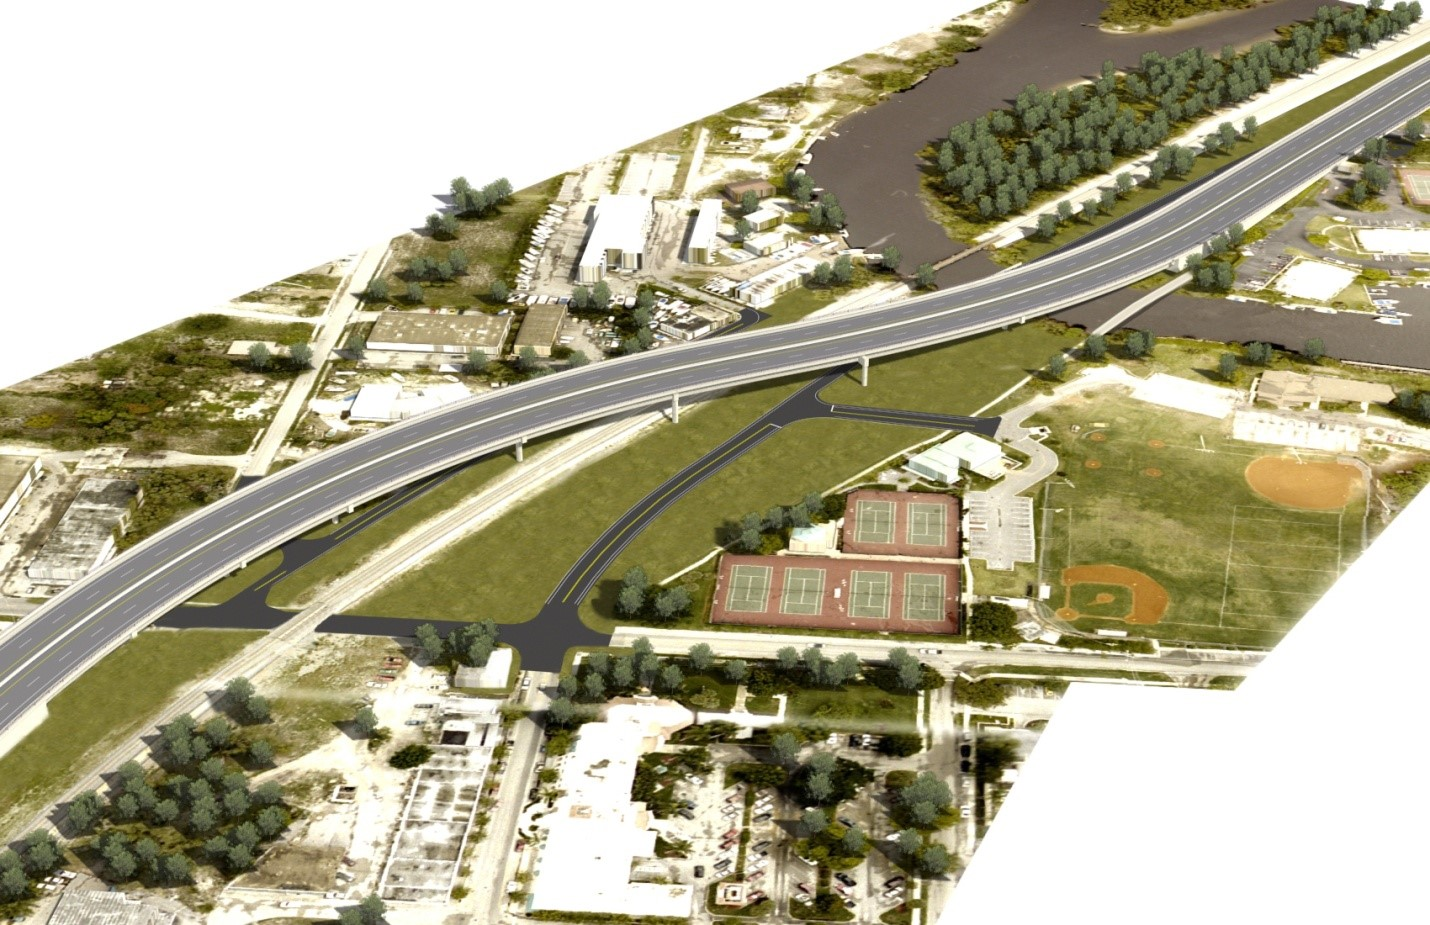
\includegraphics[width=\linewidth]{bridge-aerial.jpg}
  \caption{某桥梁项目的概念性鸟瞰图}
  \label{fig:bridge-aerial}
\end{figure}
\begin{figure}
  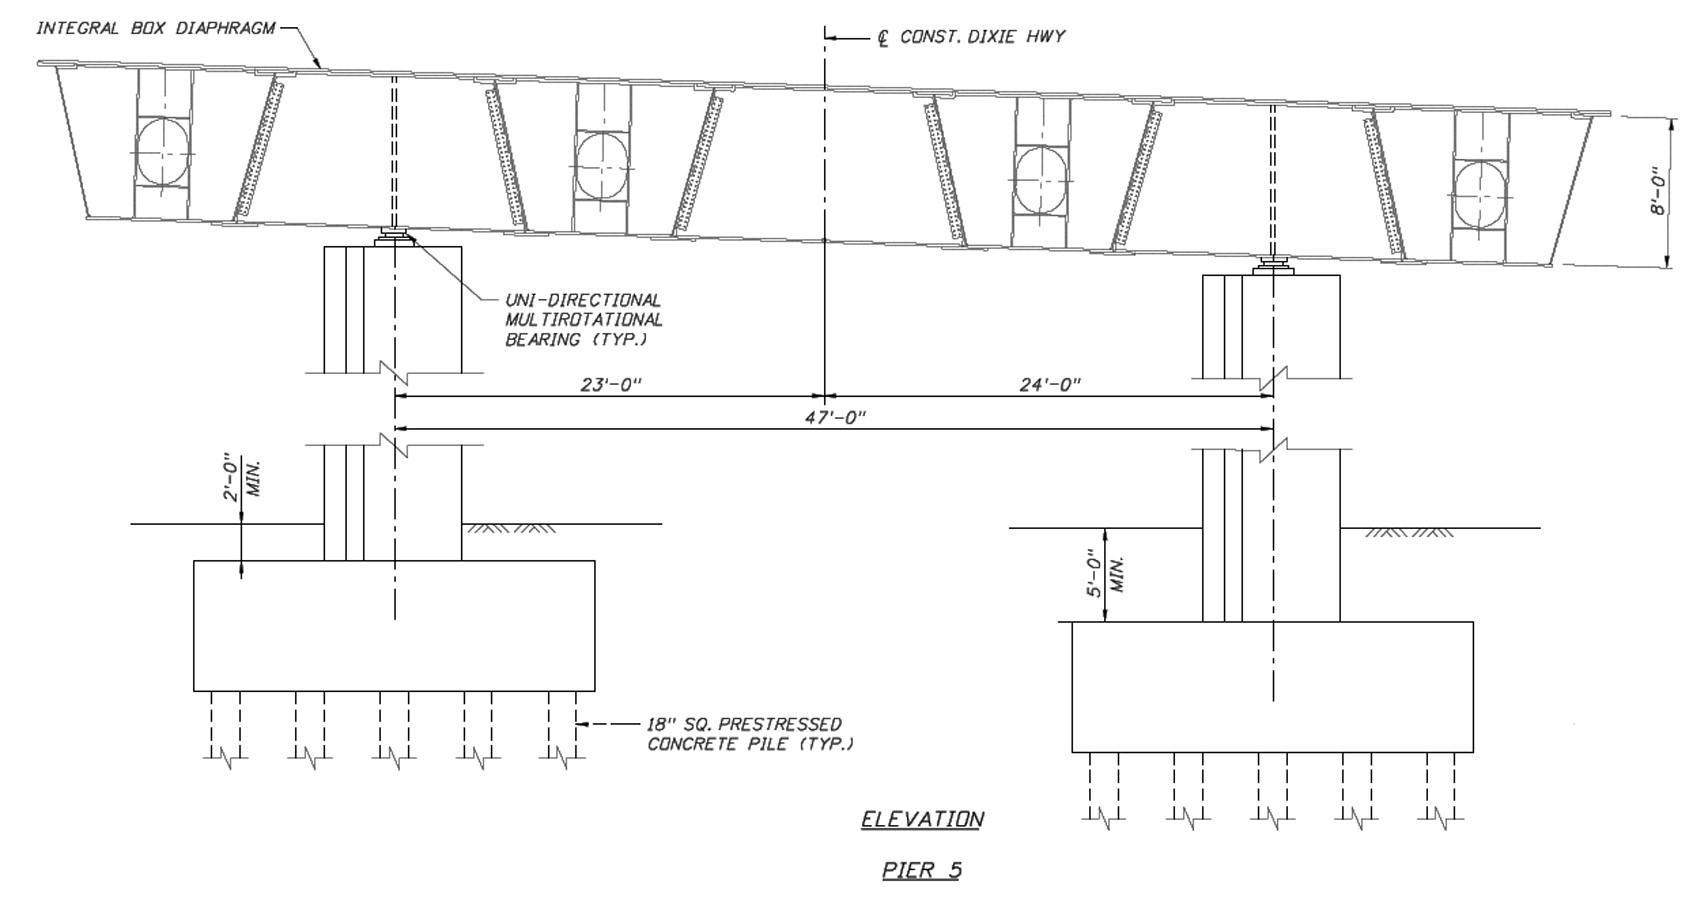
\includegraphics[width=\linewidth]{typical-section.jpg}
  \caption{典型的上部结构/下部结构布置}
  \label{fig:typical-section}
\end{figure}
\begin{figure}
  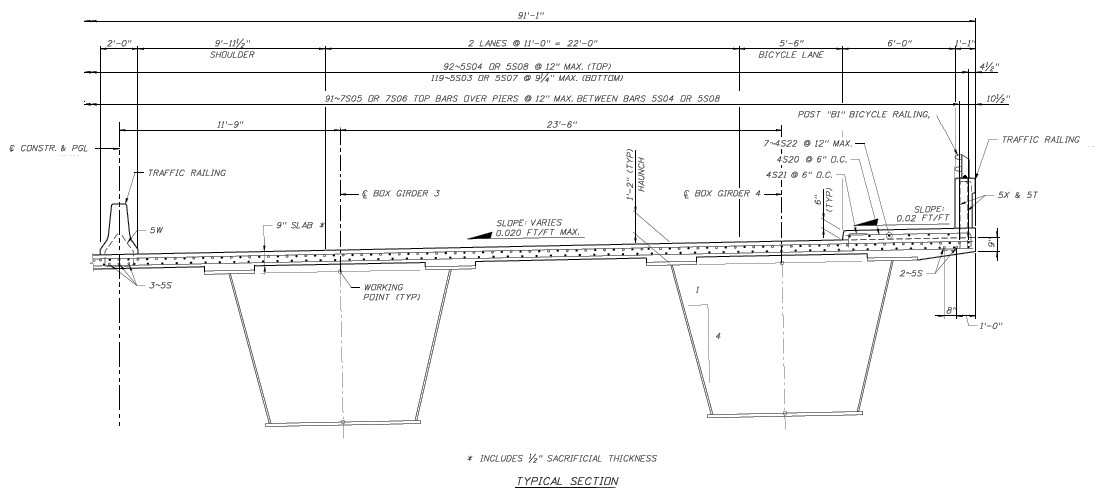
\includegraphics[width=\linewidth]{superstructure-section.jpg}
  \caption{上部结构截面——桥面——现浇方案,按 \lrfd 设计}
  \label{fig:superstructure-section}
\end{figure}

% The bridge setting includes the following characteristics, which have an influence on the service life:
桥梁的以下特性对\gls*{servicelife}有影响:
\begin{itemize}
  % \item Located in a cold environment where deicing salts are utilized, and multiple cycles of freeze/thaw are anticipated;
  \item 桥梁位于使用除冰盐的寒冷环境中,预计会有多次冻融循环;
  % \item Located in an area where studded tires are used in the winter;
  \item 桥梁位于冬季使用镶钉轮胎的区域;
  % \item Subjected to potential overloads with 20-kip tire loads in an HL93 truck configuration;
  \item 轮重 \qty{90}{kN} 的 HL93 型重载卡车引起潜在的超载;
  % \item Spans over a navigable waterway with primarily brackish conditions, and located adjacent to a park with water access for jet skis;
  \item 桥梁横跨主要为微咸水水质的通航航道,并毗邻一个公园,公园内有供水上摩托艇使用的航道;
  % \item Located near the coastline with possible salt water storm surge with potential hurricane force winds up to 150 mph wind gusts; and
  \item 桥梁位于海岸线附近,可能有咸水风暴潮,潜在飓风强度可达 \qty{240}{km/h};
  % \item Located in an area where local aggregates are subject to ASR.
  \item 桥址所在区域,当地的混凝土骨料材料会受到\acrfull{asr}影响。
\end{itemize}


% \subsection{Steps in Addressing Service Life Design}
\subsection{解决使用寿命设计的步骤}
% The first step in the process for addressing the service life design issue for bridge deck is to follow the flowchart shown in Section 4.5 of the Guide and repeated in \cref{fig:flowchart-guide}
解决桥面板\gls*{servicelife}设计问题的第一步是遵循\bkn{指南}\cref{sec:overall-strategy}中所示的流程图,此处于 \cref{fig:flowchart-guide} 重复列出。

\begin{figure}
  % \includegraphics[width=\linewidth]{graphic-file}
  \caption{\bkn{指南}\cref{chp:bridge-decks}所示流程图(\cref{fig:deck-selection-process})}\label{fig:flowchart-guide}
\end{figure}

% \cref{tab:operational-local-factors-considered} is used to extract the information needed to address the requirements of Steps 1a and 1b shown in \cref{fig:flowchart-guide}
\cref{tab:operational-local-factors-considered} 用于提取满足 \cref{fig:flowchart-guide} 中步骤 1a 和 1b 要求所需的信息。


\begin{table}
  \caption{要考虑的运营和当地因素——\cref{fig:flowchart-guide} 中的步骤 1a 和 1b}\label{tab:operational-local-factors-considered}
  % \input{tables/operational-local-factors-considered}
\end{table}

% The information shown in \cref{tab:operational-local-factors-considered} is developed from project requirements, and exemplifies the type of information necessary for layout and service life evaluation of the entire bridge system. It is well beyond that needed for simply evaluating a bridge deck, but is provided here for completeness. The pertinent issues in \cref{tab:operational-local-factors-considered}, with respect to the bridge deck, are indicated by an arrow at the right side of the table.
\cref{tab:operational-local-factors-considered} 中显示的信息是根据项目要求开发的,举例说明了整个桥梁{系统}的布局和{使用寿命}评估所需的信息类型。 它远远超出了简单评估桥面板所需的范围,但在此提供是为了完整性。 \cref{tab:operational-local-factors-considered} 中与桥面相关的相关问题在表格右侧用箭头表示。

% The next step is to identify the possible bridge deck alternatives, as indicated by Step 2 in \cref{fig:flowchart-guide}. Information provided in Section 2.3.2 of Chapter 2 and Section 4.2.1 of Chapter 4 of the Guide can be used to obtain advantages and disadvantages of various deck systems. In the case of major and complex bridges the designer may consider feasible bridge deck systems based on local preferences and experiences. In the current example, it is assumed that only the cast-in-place option is selected, as indicated in the typical girder cross section shown in Figure 1.16.
下一步是确定可能的桥面系备选方案,如\cref{fig:flowchart-guide} 中的步骤 2 所示。 本\bkn{指南}的\cref{chp:bridge-system-selection} \cref{subsec:factors-affect-deck}和第 4 章 的 4.2.1 节提供的信息可用于了解各种桥面系统的优缺点。 对于大型和复杂的桥梁,设计者可以根据当地的偏好和经验考虑可行的桥面系统。 在当前示例中,假设仅选择了现场浇筑选项,如\cref{fig:superstructure-section} 所示的典型梁横截面所示。

% Following are the steps shown in the flowchart given in Chapter 4, Section 4.4 of the Guide (Figure 4.19) and repeated in \cref{fig:flowchart-identify-factors} is the next step.
以下是\bkn{指南}\cref{chp:bridge-decks}\cref{sec:overall-strategy}(\cref{fig:mitigation-process})中给出的流程图中显示的步骤,并在 \cref{fig:flowchart-identify-factors} 重复列出。

\begin{figure}
  % \includegraphics[width=\linewidth]{graphic-file}
  % \caption{Flowchart to identify factors affecting service life. (Figure 4.19 of Guide)}
  \caption{确定影响使用寿命的因素的流程图(\bkn{指南}\cref{fig:mitigation-process}}
  \label{fig:flowchart-identify-factors}
\end{figure}

% \cref{fig:flowchart-identify-factors} aids in identifying factors that affect service life of bridge deck and in selecting possible strategies capable of mitigating the adverse effects of these factors. Identifying the factors that affect service life of bridge deck can be accomplished using the fault trees provided in \cref{chp:bridge-decks}, Section 4.2 of the Guide. Navigating through the fault tree can be simplified through the use of software. \cref{fig:screenshort} shows an example of what an Excel-based solution could look like. Using the software shown in \cref{fig:screenshort}, the user selects applicable factors from the first fault tree layer then continues through successive layers until reaching the last levels, which are depicted as circles. The items listed in each circle are the factors that will have to be addressed in the design for service life process. Each factor has the capability of reducing the service life of bridge deck. \cref{chp:bridge-decks} identifies one or more strategies capable of mitigating the effect of each particular factor listed in the circles.
\cref{fig:flowchart-identify-factors} 有助于识别影响桥面板\gls*{servicelife}的因素,并选择能够减轻这些因素不利影响的可能策略。 可以使用本\bkn{指南} \cref{chp:bridge-decks}\cref{sec:factors-influence}中提供的\gls*{faulttree}来确定影响桥面\gls*{servicelife}的因素。 通过使用软件可以简化\gls*{faulttree}的导航。 \cref{fig:screenshort} 显示了基于 \Excel\ 的解决方案的示例。 使用\cref{fig:screenshort} 中所示的软件,用户从第一个\gls*{faulttree}层选择适用的因素,然后继续通过后续层,直到到达最后一层,这些层被描绘为圆圈。 每个圆圈中列出的项目是在\gls*{servicelife}设计过程中必须解决的因素。 每个因素都有降低桥面板\gls*{servicelife}的能力。 \cref{chp:bridge-decks}确定了一种或多种能够减轻圆圈中列出的每个特定因素影响的策略。

\begin{figure}
  % \includegraphics[width=\linewidth]{graphic-file}
  \caption{Excel 工作表中\gls*{faulttree}导航的屏幕截图}\label{fig:screenshort}
\end{figure}

% \cref{fig:screenshort} shows branches of the fault tree that are applicable to the example under consideration. In the first layer, based on the project requirements, a decision is made that the service life of bridge deck can only be reduced due to deficiencies. The second layer states that either loads or natural or man-made hazards can cause bridge deck deficiencies. Both are judged to be applicable and are therefore selected. \cref{fig:screenshort} then shows the progression through the fault tree on the branch related to the factor, due to loads. The fourth layer in \cref{fig:screenshort} states that either traffic-induced loads or system-dependent loads can reduce service life of bridge deck. Again, both factors are judged to be applicable and the boxes are checked. Further, the reduction in service life of bridge deck as a result of traffic-induced loads can be caused by fatigue, overload, or wear, as depicted by the circles. All circles are applicable to the example. \cref{fig:screenshort} also identifies each factor that is capable of reducing the service life of bridge deck as a result of system-dependent loads, as shown in circles and identified as differential shrinkage, thermal, and system framing restraint. Based on project requirements, these factors are also judged applicable for consideration when addressing service life design.
\cref{fig:screenshort} 显示适用于正在考虑的示例的\gls*{faulttree}分支。第一层,根据工程要求,决定桥面因缺陷只能减少{使用寿命}。 第二层指出,负载或自然或人为的危害都可能导致桥面缺陷。 两者都被判断为适用,因此被选中。 \cref{fig:screenshort} 然后显示由于负载,\gls*{faulttree}在与该因素相关的分支上的进展。 \cref{fig:screenshort} 中的第四层指出,交通引起的负载或系统相关负载都会缩短桥面板的{使用寿命}。 同样,这两个因素都被判断为适用,并且复选框被选中。 此外,如圆圈所示,疲劳、过载或磨损可能导致交通荷载导致的桥面{使用寿命}缩短。 所有圆圈都适用于该示例。 \cref{fig:screenshort} 还确定了由于系统相关载荷而能够缩短桥面板{使用寿命}的每个因素,如圆圈所示,并确定为差异收缩、热和系统框架约束。 根据项目要求,这些因素也被判断为适用于在解决{使用寿命}设计时要考虑的因素。

% The circles in the fault tree signify:
\gls*{faulttree}中的圆圈表示:

\begin{itemize}
  \item 能够缩短使用寿命的问题;
  \item 设计者需要制定策略来缓解问题的问题。
\end{itemize}

% The strategies to address the individual items listed in each circle are provided in the Guide, in this case in Chapter 4 on bridge decks. It should also be noted that for most factors listed in the circles, the Guide identifies more than just one possible strategy.
指南中提供了解决每个圆圈中列出的各个项目的策略,在本例中是关于桥面的第 4 章。 还应注意的是,对于圆圈中列出的大多数因素,指南确定的不仅仅是一种可能的策略。

% To complete the process of navigating through the fault tree, all branches applicable to the problem need to be considered and applicable circles checked. Figure 1.20 shows the remainder of the fault tree with the “Due to Loads” branch collapsed for clarity. The decision for selecting the applicable circles is based on specific project conditions and requirements.
要完成通过\gls*{faulttree}导航的过程,需要考虑适用于问题的所有分支并检查适用的圈子。 \cref{fig:segment-fault-tree} 显示了\gls*{faulttree}的其余部分,为清楚起见,“由于负载”分支已折叠。 选择适用圈子是根据具体的项目条件和要求决定的。


\begin{figure}
  % \includegraphics[width=\linewidth]{graphic-file}
  \caption{示例中勾选了适用圆圈的\gls*{faulttree}片段}\label{fig:segment-fault-tree}
\end{figure}

% \subsection{Developing Strategies and Alternative Solutions}
\subsection{制定战略和备选解决方案}

% Once the fault tree is completed and all applicable factors are identified, the individual strategies capable of mitigating the factors can be collected. If software is utilized to work through the fault tree then this step can be automated based on the selections made. \cref{tab:mitigate-factors-strategy} summarizes the list of individual strategies capable of mitigating the factors developed for the example problem as identified as checked circles in \cref{fig:screenshort,fig:segment-fault-tree}.
一旦\gls*{faulttree}完成并确定了所有适用因素,就可以收集能够减轻这些因素的个别策略。如果使用软件来处理\gls*{faulttree},则可以根据所做的选择自动执行此步骤。\cref{tab:mitigate-factors-strategy} 总结了能够减轻为示例问题开发的因素的单个策略列表,这些因素在 \cref{fig:screenshort,fig:segment-fault-tree} 中被标识为选中的圆圈。

\begin{table}
  \caption{能够减轻影响示例问题使用寿命的因素的个别策略列表}\label{tab:mitigate-factors-strategy}
  % \input{tables/filename}
\end{table}

% At this point, the designer has developed a complete list of strategies that can be used for mitigating various factors capable of affecting the service life of bridge deck, based on project requirements. \cref{tab:mitigate-factors-strategy} also provides sections of the Guide that the user can refer to for more information, and lists advantages and disadvantages of the defined strategies. Some of the strategies may contradict each other while others may result in similar results. Intentionally, the Guide does not provide a single strategy or attempt to identify the best strategy. In many cases strategies to mitigate the individual factors capable of reducing service life are context sensitive, meaning that the best strategy is very much dependent on such factors as local practice, environment, or owner preferences.
至此,设计师已经根据项目要求制定了一份完整的策略清单,可用于缓解影响桥面板使用寿命的各种因素。 \cref{tab:mitigate-factors-strategy} 还提供了用户可以参考以获取更多信息的指南部分,并列出了已定义策略的优点和缺点。 一些策略可能相互矛盾,而另一些策略可能会产生相似的结果。 有意地,该指南不提供单一策略或尝试确定最佳策略。 在许多情况下,减轻能够缩短使用寿命的个别因素的策略是上下文敏感的,这意味着最佳策略在很大程度上取决于当地实践、环境或业主偏好等因素。

% As mentioned, some of the strategies may contradict each other and some may be more preferable based on local practices or owner preferences. Consequently, the next step for the designer is to select strategies that are desirable for each factor affecting the service life. \cref{tab:strategy-deck-alternatives} shows a narrower list of strategies extracted from the complete list given in \cref{tab:mitigate-factors-strategy}. The first row in \cref{tab:strategy-deck-alternatives} shows the applicable factors that can reduce the service life of bridge deck under consideration. These factors were obtained by navigating through branches of the fault tree.
如前所述,一些策略可能相互矛盾,而根据当地实践或所有者偏好,一些策略可能更可取。 因此,设计师的下一步是选择适合影响使用寿命的每个因素的策略。\cref{tab:strategy-deck-alternatives} 显示了从 \cref{tab:mitigate-factors-strategy} 中给出的完整列表中提取的更窄的策略列表。\cref{tab:strategy-deck-alternatives} 中的第一行显示了可能会缩短所考虑的桥面板使用寿命的适用因素。 这些因素是通过浏览\gls*{faulttree}的分支获得的。

\begin{table}
  \caption{桥面系备选方案专用策略列表}\label{tab:strategy-deck-alternatives}
  % \input{tables/filename}
\end{table}


% In developing the information shown in \cref{tab:strategy-deck-alternatives}, the designer may consider many factors and ensure that there are no contradicting strategies. For instance, appropriate concrete mix is specified as one strategy to address wear, differential shrinkage, freeze/thaw, humidity, and ASR/ACR. The designer must ensure that a concrete mix capable of addressing all of these issues can be developed. Otherwise, for a particular factor the designer may be forced to use another strategy. As an example for differential shrinkage, a low modulus of elasticity concrete is needed, whereas for wear, a high modulus of elasticity is needed. Consequently, to address wear and differential shrinkage, the same concrete mix cannot be used to mitigate both factors, and within a given deck alternative, one of these factors should be mitigated using a different strategy.
在开发 \cref{tab:strategy-deck-alternatives} 中显示的信息时,设计者可能会考虑许多因素并确保没有矛盾的策略。 例如,适当的混凝土混合物被指定为解决磨损、收缩差异、冻结/解冻、湿度和 ASR/ACR 的一种策略。 设计师必须确保能够开发出能够解决所有这些问题的混凝土组合。 否则,对于特定因素,设计者可能被迫使用另一种策略。 例如,对于不同的收缩,需要低弹性模量的混凝土,而对于耐磨,则需要高弹性模量。 因此,为了解决磨损和收缩差异,不能使用相同的混凝土混合物来减轻这两个因素,并且在给定的甲板替代方案中,应该使用不同的策略来减轻其中一个因素。

% The next step in the process is to develop possible deck alternatives that meet both LRFD Specifications requirements and Guide requirements.
该过程的下一步是开发满足 \lrfd 要求和\bkn{指南}要求的可能桥面系备选方案。

% Using the information provided in \cref{tab:strategy-deck-alternatives} and ensuring there is no contradiction among strategies to mitigate various factors, \cref{tab:alternative-aashto-guide} shows four possible deck alternatives capable of mitigating all factors affecting the service life of the bridge for the example under consideration. The four alternatives shown in \cref{tab:alternative-aashto-guide} are project specific solutions. It is also possible to automate this step by first identifying all possible deck alternatives based on all possible combinations of strategies listed in \cref{tab:strategy-deck-alternatives} and then eliminating those judged not feasible, because of contradiction among strategies.
使用 \cref{tab:strategy-deck-alternatives} 中提供的信息并确保减轻各种因素的策略之间没有矛盾,\cref{tab:alternative-aashto-guide} 显示了四种可能的套牌替代方案,能够减轻所有因素 影响正在考虑的例子中桥梁的使用寿命。 \cref{tab:alternative-aashto-guide} 中显示的四个备选方案是项目特定的解决方案。 也可以通过首先根据 \cref{tab:strategy-deck-alternatives} 中列出的所有可能的策略组合识别所有可能的套牌替代方案,然后消除那些由于策略之间的矛盾而被判断为不可行的套牌替代方案,从而自动执行此步骤。

\begin{table}
  \caption{开发同时满足 \acrshort{aashto} 和\bkn{指南}要求的桥面系备选方案}\label{tab:alternative-aashto-guide}
  % \input{tables/filename}
\end{table}


% For each alternative shown in \cref{tab:alternative-aashto-guide}, rows two through 11 show the service life design factors identified in \cref{tab:strategy-deck-alternatives} and corresponding strategies selected for each alternative. Incorporating all of the select strategies listed in rows 2 through 11 for each of the four alternatives results in modified deck configurations shown in row 13 of \cref{tab:alternative-aashto-guide}. Development of the four deck alternatives signifies the completion of step 4a shown in \cref{fig:flowchart-identify-factors}. It should be mentioned that strategies listed in \cref{tab:strategy-deck-alternatives} could lead to the development of additional deck alternatives. However, for the sake of simplicity, only four alternatives are shown in \cref{tab:alternative-aashto-guide}.
对于 \cref{tab:alternative-aashto-guide} 中显示的每个备选方案,第 2 行到 11 行显示了 \cref{tab:strategy-deck-alternatives} 中确定的使用寿命设计因素以及为每个备选方案选择的相应策略。 将第 2 行到第 11 行中列出的所有选择策略合并到四个备选方案中的每一个,会导致修改后的套牌配置,如 \cref{tab:alternative-aashto-guide} 的第 13 行所示。 四副套牌替代品的开发标志着 \cref{fig:flowchart-identify-factors} 中所示的步骤 4a 的完成。 应该提到的是,在 \cref{tab:strategy-deck-alternatives} 中列出的策略可能会导致开发额外的套牌替代方案。 然而,为了简单起见,\cref{tab:alternative-aashto-guide} 中只显示了四个备选方案。


% The first option shown in \cref{tab:alternative-aashto-guide}, column 2, represents a design that meets the strength requirements stated in LRFD Specifications. The total deck thickness is 8 in., with no considerations for any of the factors capable of reducing the service life. The main feature of the first alternative, Alt. 1 in \cref{tab:alternative-aashto-guide}, is having impermeable concrete, with 5\% silica fume and 10\% fly ash. The addition of fly ash is assumed to impact the rate of reduction in the diffusivity of concrete, a parameter used in estimating the time to initiate corrosion.
\cref{tab:alternative-aashto-guide} 第 2 列中显示的第一个选项表示满足 LRFD 规范中规定的强度要求的设计。 甲板总厚度为 8 英寸,未考虑任何可能缩短使用寿命的因素。 第一个替代方案的主要特征,Alt。 \cref{tab:alternative-aashto-guide} 中的 1,具有防渗混凝土,含 5\% 硅粉和 10\% 粉煤灰。 假设添加飞灰会影响混凝土扩散系数的降低速率,这是用于估计开始腐蚀时间的参数。

% The second alternative, Alt. 2 in \cref{tab:alternative-aashto-guide}, relies mainly on the use of stainless steel reinforcement, in this case Grade 316 stainless steel, to prevent corrosion. Alternative 3, Alt. 3 in \cref{tab:alternative-aashto-guide}, uses regular concrete with increased cover to delay the time to initiate the corrosion. Finally, the fourth alternative, Alt. 4 in \cref{tab:alternative-aashto-guide}, uses a membrane and overlay to address corrosion.
第二种选择,Alt。 \cref{tab:alternative-aashto-guide} 中的 2,主要依靠使用不锈钢加固,在本例中为 316 级不锈钢,以防止腐蚀。 备选方案 3,备选方案。 3 在 \cref{tab:alternative-aashto-guide} 中,使用增加覆盖层的普通混凝土来延迟开始腐蚀的时间。 最后,第四种选择,Alt。 \cref{tab:alternative-aashto-guide} 中的 4,使用膜和覆盖层来解决腐蚀问题。

% All alternatives use increased thickness to address overload, increasing the deck thickness by 0.5 in. \cref{tab:alternative-aashto-guide} also addresses additional strategies capable of reducing service life of the various alternatives.
所有备选方案都使用增加厚度来解决过载问题,将甲板厚度增加 0.5 英寸。\cref{tab:alternative-aashto-guide} 还解决了能够缩短各种备选方案使用寿命的其他策略。


% \subsection{Evaluating Alternatives}
\subsection{评估备选方案}
% As shown in \cref{fig:flowchart-guide}, the next step is predicting the service life of each alternative, Step 5 in \cref{fig:flowchart-guide}, and comparing it to the design service life of the bridge system, as specified by the owner and project requirements. Based on the outcome, the development of rehabilitation or replacement requirements, Step 5a in \cref{fig:flowchart-guide}, and a maintenance plan, Step 6 in \cref{fig:flowchart-guide}, may be necessary. The last step for the bridge deck alternative under consideration, as shown in \cref{fig:flowchart-guide}, Step 7, is to perform life cycle cost analysis for comparison.
如 \cref{fig:flowchart-guide} 所示,下一步是预测每个备选方案的使用寿命,\cref{fig:flowchart-guide} 中的第 5 步,并将其与桥梁系统的设计使用寿命进行比较 ,由业主和项目要求指定。 根据结果,可能需要制定修复或更换要求(\cref{fig:flowchart-guide} 中的步骤 5a)和维护计划(\cref{fig:flowchart-guide} 中的步骤 6)。如 \cref{fig:flowchart-guide} 第 7 步所示,正在考虑的桥面板备选方案的最后一步是执行生命周期成本分析以进行比较。

% As described in \cref{chp:bridge-system-selection} on system selection, the designer must also consider the interaction that might exist between various parts of the bridge. This step is not covered for this example.
正如 \cref{chp:bridge-system-selection} 中关于\gls*{system}选择的描述,设计者还必须考虑桥梁各部分之间可能存在的相互作用。此示例不包括此步骤。

% The potential service life of each deck alternate can be calculated based on the assumption that the main mode of deterioration is ingress of chloride into concrete, which can result in corrosion of reinforcement. One approach is to use the solution to Fick's second law as shown below.
每个桥面系备选方案的潜在使用寿命可以基于以下假设来计算:主要的劣化模式是氯离子对混凝土的渗透,这会导致钢筋腐蚀。一种方法是使用菲克第二定律的解决方案,如下所示。

% In a one-dimensional case, Fick's Law can be expressed and illustrated as follows:
在一维情况下,菲克定律可以表达如下:
\begin{equation}
  \label{eq:ficks-law}
  C(x,t)=C_0\left(1- \erf \frac{x}{2\sqrt{D_\text{c}t}} \right)
\end{equation}
\begin{EqDesc}{C(x,t)}
  \item[C(x,t)] 深度 $x$ 处在时间 $t$ 时的氯离子浓度;
  \item[C_0] 表明氯离子浓度(\unit{kg/m^3});
  \item[D_\text{c}] 氯离子扩散常数(\unit{cm^2/yr});
  \item[\erf] 误差函数(来自标准数学表)。
\end{EqDesc}

% The use of Fick's Law to determine the time of corrosion initiation is described in \cref{chp:corrosion-of-steel-rc-bridge}\cref{sec:description-corrosion}, of the Guide. \cref{eq:ficks-law} can be used to assess ingress of chloride through the concrete cover. As an example, \cref{fig:chloride-concentration} indicates the type of information that can be developed, which shows chloride concentration through the deck thickness for three time periods, after a deck is cast.
本指南的\cref{chp:corrosion-of-steel-rc-bridge}\cref{sec:description-corrosion}中描述了使用菲克定律确定腐蚀开始时间。\cref{eq:ficks-law} 可用于评估氯离子通过混凝土保护层的侵入。例如,\cref{fig:chloride-concentration} 表示可以开发的信息类型,它显示了桥面板浇筑后三个时间段内整个桥面板厚度中的氯离子浓度。

\begin{figure}
  % \includegraphics[width=\linewidth]{graphic-file}
  \caption{混凝土中的氯化物浓度与时间的关系}\label{fig:chloride-concentration}
\end{figure}

% The information shown in \cref{fig:chloride-concentration} can be used to predict the time when corrosion will be initiated, which in turn can be used to estimate the service life of the bridge deck, if corrosion of reinforcement is the main mode of deterioration. The Fick's law in this case is the deterioration model.
\cref{fig:chloride-concentration} 中显示的信息可用于预测腐蚀开始的时间,如果钢筋腐蚀是主要模式,这又可用于估计桥面板的使用寿命 的恶化。 这种情况下的菲克定律是退化模型。

% To complete the example, Life-365, a free program developed by the concrete industry, is used to conduct the life cycle cost analysis and assist in selecting an optimum solution. Life-365 uses a finite-difference approach to solve Fick's second law and to estimate the time to initiation of corrosion. Other approaches such as error function solution to Fick's second law, \cref{eq:ficks-law}, could also be used.
为了完成这个例子,\gls{life365} 是一个由混凝土行业开发的免费程序,用于进行生命周期成本分析并协助选择最佳解决方案。 \gls{life365} 使用有限差分法求解菲克第二定律并估计腐蚀开始的时间。也可以使用其他方法,例如菲克第二定律的误差函数解法 \cref{eq:ficks-law}。

% The solution to Fick's second law estimates the time to initiation of corrosion, $t_\text{i}$. For the example, it is assumed (assumption within Life-365) that once the corrosion is initiated, the time to propagate the corrosion to the point at which repair is needed, $t_\text{r}$ , is a constant six years, regardless of concrete mix used. Following the time period, $t_\text{i} + t_\text{r}$, Life-365 assumes repair action at set time intervals, say every 10 or 20 years, and set cost per unit area in square feet. Further, within each repair cycle, it is assumed that only a portion of the deck area will be repaired. For instance, within each repair cycle only 10\% or 20\% of the deck will need repair.
菲克第二定律的解估计了腐蚀开始的时间 $t_\text{i}$。 例如,假设(\gls{life365} 中的假设)一旦腐蚀开始,腐蚀传播到需要修复的点的时间 $t_\text{r}$ 是恒定的六年 , 无论使用何种混凝土混合物。 在时间段 $t_\text{i} + t_\text{r}$ 之后,\gls{life365} 会按设定的时间间隔(比如每 10 年或 20 年)采取维修行动,并设定单位面积的成本(以平方英尺为单位)。 此外,在每个维修周期内,假设只有一部分甲板区域将被维修。 例如,在每个维修周期内,只有 10\% 或 20\% 的甲板需要维修。

% The time to initiate corrosion depends on concrete mix and preventive measures, such as use of stainless steel, concrete cover, or membranes. Life-365 follows the guidance and terminology in ASTM E-917 Standard Practice for Estimating the Life Cycle Cost of Building System. The final number that can be used to select the optimal deck alternative can be the life cycle cost, which is the initial cost plus the present value of all future rehabilitation costs over the desired service life, in this case 100 years.
开始腐蚀的时间取决于混凝土混合料和预防措施,例如使用不锈钢、混凝土覆盖层或膜。 \gls{life365} 遵循 ASTM E-917 建筑系统生命周期成本估算标准实践中的指导和术语。 可用于选择最佳甲板备选方案的最终数字可以是生命周期成本,即初始成本加上预期使用寿命(在本例中为 100 年)内所有未来修复成本的现值。

% \cref{tab:input-parameters} shows the input parameters used within \gls{life365} to conduct a life cycle cost analysis for each of the four alternatives shown in \cref{tab:alternative-aashto-guide}.
\cref{tab:input-parameters} 显示了 \gls{life365} 中使用的输入参数,用于对 \cref{tab:alternative-aashto-guide} 中显示的四种备选方案中的每一种进行生命周期成本分析。

\begin{table}
  \caption{\gls{life365}中所有四种备选方案的输入参数}\label{tab:input-parameters}
  % \input{tables/filename}
\end{table}

% It is assumed that the bridge is located in Boston, Massachusetts; has a required service life of the deck of 100 years; and, for the sake of comparison, a total surface area of the deck of 10,000 square ft. \cref{tab:input-parameters} also shows the yearly temperature profile used. The diffusion coefficient and ingress of chloride are influenced by temperature fluctuation. The input parameters shown in \cref{tab:input-parameters} are applicable to all four alternatives shown in \cref{tab:alternative-aashto-guide}. The specific input and end results for each alternative are shown in \cref{tab:parameter-each-alternative}.
假设这座桥位于马萨诸塞州的波士顿;要求甲板的使用寿命为100年;并且,为了进行比较,甲板的总表面积为 10,000 平方英尺。\cref{tab:input-parameters} 还显示了所使用的年度温度曲线。扩散系数和氯化物的进入受温度波动的影响。\cref{tab:input-parameters} 中显示的输入参数适用于\cref{tab:alternative-aashto-guide} 中显示的所有四个备选方案。每个备选方案的具体输入和最终结果显示在\cref{tab:parameter-each-alternative} 中。

\begin{table}
  % \caption{Parameters Specific to Each Alternative}
  \caption{每个备选方案特定的参数}
  \label{tab:parameter-each-alternative}
  % \input{tables/filename}
\end{table}

% As indicated in \cref{tab:parameter-each-alternative}, alternatives 1, 2, 3, and 4 use the same concrete mix, hereafter referred to as regular mix, which was used for the base option designed in accordance with LRFD Specifications (option designated as AASHTO Design in \cref{tab:alternative-aashto-guide}). Alternative 1 uses 5\% silica fume to make the concrete impermeable. Alternative 2 uses stainless steel. Alternative 3 uses increased concrete cover to delay the adverse effects of corrosion. Alternative 4 uses a membrane and overlay.
如 \cref{tab:parameter-each-alternative} 所示,备选方案 1、2、3 和 4 使用相同的混凝土配合比,以下称为常规配合比,用于根据 LRFD 规范设计的基础选项 (在 \cref{tab:alternative-aashto-guide} 中指定为 AASHTO 设计的选项)。 备选方案 1 使用 5\% 硅粉使混凝土不透水。 备选方案 2 使用不锈钢。 备选方案 3 使用增加的混凝土保护层来延迟腐蚀的不利影响。 备选方案 4 使用薄膜和覆盖层。

% Following is a brief description of the results for each alternative.
以下是对每个备选方案的结果的简要说明。


% \paragraph*{Deck Design Based on LRFD Specifications}
\paragraph*{基于 \lrfd 的桥面板设计}
% As shown in \cref{tab:parameter-each-alternative}, in the case of the AASHTO base design, corrosion starts after 6.6 years (shown as Initiation). Thereafter, the propagation of corrosion to the point of needed repair is 6 years. At the end of 12.6 years, the repair and maintenance actions are assumed to start and continue every 10 years, during which 20\% of the surface area is repaired. These assumptions are used for the sake of demonstration and will vary based on various DOT preferences and practices. \cref{fig:total-life-cost} shows the total life cycle cost based on present value.
如 \cref{tab:parameter-each-alternative} 所示,在 \gls{aashto} 基础设计的情况下,腐蚀在 6.6 年后开始(显示为初始)。 此后,腐蚀传播到需要修复的点为 6 年。 在 12.6 年末,假设维修和保养行动每 10 年开始并持续一次,期间维修 20\% 的表面积。 这些假设用于演示目的,并且会根据各种 DOT 偏好和实践而有所不同。 \cref{fig:total-life-cost} 显示基于现值的总生命周期成本。

\begin{figure}
  % \includegraphics[width=\linewidth]{graphic-file}
  \caption{基于 \acrshort{lrfd} 规范的设计的总生命周期成本}\label{fig:total-life-cost}
\end{figure}

% The total life cycle cost for the AASHTO based design is \$774,676, which is shown in the last row of \cref{tab:parameter-each-alternative}. An inflation rate of 1.6\% and a discount rate of 2\% were used in developing the total life cycle cost. As indicated in \cref{tab:parameter-each-alternative}, the initial cost of AASHTO base design is the lowest of the alternatives (\$37, 215). However, the total life cycle cost is the highest (\$774,676). It should also be mentioned that these life cycle cost analyses ignore the user costs, or any other cost to society during repair and closure to traffic, and these costs can be significant.
基于 AASHTO 的设计的总生命周期成本为 774,676 美元,显示在 \cref{tab:parameter-each-alternative} 的最后一行。 计算总生命周期成本时使用了 1.6\% 的通货膨胀率和 2\% 的贴现率。 如 \cref{tab:parameter-each-alternative} 所示,AASHTO 基础设计的初始成本是所有备选方案中最低的 (\$37, 215)。 但是,总生命周期成本最高(\$774,676)。 还应该提到的是,这些生命周期成本分析忽略了用户成本,或在维修和关闭交通期间对社会造成的任何其他成本,这些成本可能是巨大的。


% \paragraph*{Alternative 1}
\paragraph*{备选方案 1}
% This alternative uses impermeable concrete by incorporating 5\% silica Fume in the mix. As a result, the initial unit cost of concrete is assumed to increase by ten dollars per cubic yard. The initiation of corrosion starts at 34.8 years after casting and the propagation phase lasts six years. Therefore, after 40.8 years the repair procedure is assumed to stat. It is assumed that the repair procedure is to be conducted every 10 years and during each repair cycle, 10\% of the surface area is assumed to need repair. Other repair alternatives can consist of complete replacement of deck every 40 years. The total life cycle cost of Alternative 1 for the assumptions made is \$277, 550, as shown in \cref{tab:parameter-each-alternative}. The initial cost of Alternative 1, \$44,645, is slightly higher than initial cost for AASHTO base design (\$37,215).
该替代方案通过在混合物中加入 5\% 硅粉来使用不透水混凝土。 因此,假设混凝土的初始单位成本每立方码增加 10 美元。 腐蚀开始于铸造后 34.8 年,传播阶段持续 6 年。 因此,在 40.8 年后,修复程序被假定为 stat。 假定维修程序每 10 年进行一次,并且在每个维修周期内,假定 10\% 的表面积需要维修。 其他维修方案包括每 40 年完全更换一次甲板。 如 \cref{tab:parameter-each-alternative} 中所示,根据所做的假设,备选方案 1 的总生命周期成本为 277 美元、550 美元。 备选方案 1 的初始成本为 44,645 美元,略高于 AASHTO 基础设计的初始成本(37,215 美元)。

% \paragraph*{Alternative 2}
\paragraph*{备选方案 2}
% This alternative uses Grade 316 stainless steel to address the corrosion of reinforcement issue. The time to initiation of corrosion for this alternative is more than 100 years and consequently no repair action is needed. The initial cost of using stainless steel is the highest among all alternatives (\$152,753). However, the total life cycle cost associated with Alternative 2, \$152,753 as shown in \cref{tab:parameter-each-alternative}, is the lowest among all alternatives.
该替代方案使用 316 级不锈钢来解决钢筋腐蚀问题。 这种替代品的腐蚀开始时间超过 100 年,因此不需要采取任何修复措施。 使用不锈钢的初始成本是所有替代品中最高的(\$152,753)。 然而,与备选方案 2 相关的总生命周期成本为 \cref{tab:parameter-each-alternative} 中所示的 \$152,753,是所有备选方案中最低的。

% \paragraph*{Alternative 3}
\paragraph*{备选方案 3}

% This alternative uses increased cover to delay the initiation of corrosion. Using increased cover delays the corrosion initiation from for AASHTO base design from 6.6 years to 15.2 years, as indicated in \cref{tab:parameter-each-alternative}. The total cost of Alternative 3 is relatively high, \$691,114. There does not seem to be much benefit in using this alternative, especially considering that increasing the concrete cover will subject the substructure and foundations to higher dead loads.
该替代方案使用增加的覆盖层来延迟腐蚀的开始。 使用增加的覆盖层可将 AASHTO 基础设计的腐蚀起始时间从 6.6 年延迟到 15.2 年,如 \cref{tab:parameter-each-alternative} 中所示。 备选方案 3 的总成本相对较高,为 \$691,114。 使用这种替代方案似乎没有太大好处,特别是考虑到增加混凝土保护层会使下部结构和地基承受更高的恒载。


% \paragraph*{Alternative 4}
\paragraph*{备选方案 4}

% Alternative 4 uses a membrane and overlay to prevent corrosion of reinforcement. The total deck thickness is only 8.5 in. compared to 9 in. and 10 in. used for Alternatives 1, 2 and 3. The repair cost per square foot for this alternative is assumed to be lower at \$20/ft2 as compared to \$50/ft2 for others when a membrane is used. It is assumed that a high quality membrane at \$7/ft2 is used and that it will last 75 years. Consequently, the repair will involve replacing damaged overlay areas, which are assumed to be 5\% of the total surface area during each repair cycle—every 10 years after 28.4 years of first installation (see \cref{tab:parameter-each-alternative}). At \$172,252, the total life cycle cost of this alternative, using membrane, is very low, while the initial cost (\$39,541 + \$70,000) is more than twice the AASHTO base design of \$37,215. It should also be mentioned that the use of a membrane could be much more economical than that indicated by this example. For instance, the calculation leads to the conclusion that corrosion will start after 28.4 years, which is not realistic. The concrete deck below the membrane could last a long time without any need for repair, and any needed repair action would only be for replacing the thin overlay, which could be achieved quickly with minimal interruption to traffic. These factors are not considered in conducting the life cycle cost analysis for this alternative.
备选方案 4 使用薄膜和覆盖层来防止钢筋腐蚀。 与备选方案 1、2 和 3 所用的 9 英寸和 10 英寸相比,总甲板厚度仅为 8.5 英寸。与 \ 使用膜时,其他人为 50 美元/平方英尺。 假设使用了 7 美元/平方英尺的高质量膜,并且它将持续 75 年。 因此,维修将涉及更换损坏的覆盖区域,假设在每个维修周期中更换损坏的覆盖区域 - 在首次安装 28.4 年后每 10 年更换一次(参见 \cref{tab:parameter-each-alternative}). 这种使用膜的替代方案的总生命周期成本为 172,252 美元,非常低,而初始成本(39,541 美元 + 70,000 美元)是 AASHTO 基础设计 37,215 美元的两倍多。 还应该提到的是,使用膜可能比本例所示的更经济。 例如,计算得出28.4年后开始腐蚀的结论,这是不现实的。 膜下的混凝土桥面可以持续很长时间而无需维修,任何需要的维修行动只是更换薄的覆盖层,可以在交通中断最少的情况下快速完成。 在对该备选方案进行生命周期成本分析时未考虑这些因素。

% \subsection{Summary and Conclusion}
\subsection{总结与结论}
% The table below provides a summary of results for all alternatives. Using this information it is feasible to conclude that use of stainless steel or membrane plus overlay can provide the best economy.
\cref{tab:alternative-summary} 汇总了所有备选方案的结果。使用此信息可以得出结论,使用不锈钢或加设薄膜覆盖层可以提供最佳的经济性。

\begin{table}
  \caption{备选方案汇总}\label{tab:alternative-summary}
  \begin{tblr}{
  colspec={c X[l] Q[r,si={table-format=7.0}] Q[r,si={table-format=7.0}]},
  row{1}={c,bg=genfg,fg=white,font=\bfseries,guard}
}
备选方案 & 解决腐蚀的主要方法        & 初始成本(\$)& 全生命周期成本(\$)\\
\acrshort{aashto} 基本设计 & N/A     & 37215    & 774676          \\
 方案 1      & 使用硅粉的抗渗混凝土  & 44645    & 277550          \\
 方案 2      & 使用 316 号不锈钢     & 152753   & 152753          \\
 方案 3      & 增大混凝土保护层      & 46519    & 691114          \\
 方案 4      & 使用薄膜和覆盖层      & 109541   & 172252          \\
\end{tblr}
\end{table}

% \section{Future Development of the Guide}
\section{《指南》的未来发展}
% The Guide provides a general, comprehensive framework for designing new bridges and rehabilitating existing bridges for service life. The approach presented by the Guide is flexible and can be adapted as new information becomes available. The Guide also provides a platform for developing customized manuals by individual State DOTs or for developing a customized and systematic approach for service life design of major and complex bridges.
本\bkn{指南}为设计新建桥梁和修复既有桥梁的\gls{servicelife}提供了一个通用的综合框架。本\bkn{指南}提出的方法是灵活的,可以根据新信息的出现进行调整。本\bkn{指南}还提供了一个平台,供各州\acrlong{dot}开发定制手册,或为大型复杂桥梁的\gls{servicelife}设计开发定制的系统方法。

% Design for service life is a context sensitive problem and local agency practices and preferences are important. Customizing the Guide can be achieved by using the general framework outlined in these pages and incorporating strategies and solutions preferred by each DOT for factors affecting service life of their bridges.
\gls{servicelife}设计是一个语境敏感的问题,即,当地机构的做法和偏好很重要。可以通过使用这概述的一般框架并结合每个\gls{dot}首选的措施和解决方案来定制\bkn{指南},以解决影响其桥梁\gls{servicelife}的因素。

% One of the challenges in developing true service life design is the lack of reliable, available deterioration models that are based on either field data or laws of physics governing the deterioration. Several studies are underway to develop deterioration models for various bridge elements, components, and subsystems. Such information can be incorporated into the Guide as they become available. These models are needed to further develop reliable life cycle cost analysis.

开发真实\gls*{servicelife}设计的挑战之一是缺乏基于现场数据或控制\gls*{deterioration}的物理定律的可靠、可用的\gls*{deterioration}模型。目前正在进行多项研究,以开发各种桥梁\gls{element}、\gls{component}和\gls{subsystem}的\gls*{deterioration}模型。此类信息可在可用时纳入\bkn{指南}。需要这些模型来进一步开发可靠的生命周期成本分析。

% There is a need to develop specific life cycle cost analysis tools dedicated to bridges, with the ability to incorporate user costs where applicable. These tools must be flexible enough to allow incorporating new information and deterioration models as they become available.

需要开发专用于桥梁的特定生命周期成本分析工具,并能够在适用的情况下纳入用户成本。这些工具必须足够灵活,以便在新信息和\gls*{deterioration}模型可用时纳入其中。

% There is a further need to develop more comprehensive examples, which take into account the interaction between solutions that may seem appropriate for an individual bridge element, component, or subsystem when viewed in isolation, and yet are less than optimum when considering service life solutions for the combined bridge system.

还需要开发更全面的示例,这些示例考虑了解决方案之间的相互作用,这些解决方案在孤立地看时似乎适合于单个桥梁\gls{element}、\gls{component}或\gls{subsystem},但在考虑\gls{servicelife}解决方案时却不是最佳的联合桥梁\gls{system}。

% Finally, the significant amount of information provided in the Guide is time consuming to comprehend in its entirety. There is a need to automate the use of the Guide by developing tools that would facilitate navigating through all of the included information.

最后,\bkn{指南}中提供的大量信息需要花费大量时间才能完全理解。有必要通过开发有助于浏览所有包含信息的工具来自动使用\bkn{指南}。
 % 英文输入完成,差图片和表格,文字待修改。
% \chapter{Bridge System Selection}\label{chp:bridge-system-selection}
\chapter{桥梁\glsentrytext{system}的选择}\label{chp:bridge-system-selection}
% \section{Introduction}
\section{简介}
% Selecting the proper bridge system and incorporating service life design principles into the planning and design process are critical steps in achieving long-term bridge service life. As it is more cost effective to address service life at the design stage, the design for service life must be approached in a systematic, coherent manner.
选择合适的桥梁\gls*{system}并将\gls*{servicelife}设计原则纳入规划和设计过程是实现桥梁较长\gls*{servicelife}的关键步骤。由于在设计阶段解决\gls*{servicelife}问题更具成本效益,因此必须以系统、连贯的方式进行\gls*{servicelife}设计。

% This chapter provides essential information, steps, and guidelines for selecting and designing optimum bridge systems for both existing and new bridges. More specific details for certain bridge elements, components, subsystems, and materials are provided in other chapters and are referenced herein.
本章提供了为既有桥梁和新建桥梁选择和设计最佳桥梁\gls*{system}的基本信息、步骤和指南。此处引用了某些桥梁\gls*{element}、\gls*{component}、\gls*{subsystem}和材料的细节,其具体内容在将其他章节中展开。

% Commonly-used bridge systems are examined along with their associated challenges and solutions, and the focus is on durability and service life. The discussion covers conventional bridge systems and newer, innovative systems involving accelerated and modular construction. Steel and concrete bridge superstructure types are discussed, but when possible they are not directly compared. Instead, the discussion addresses various service life issues within both steel and concrete superstructures.
本章对常用的桥梁\gls*{system}及其面临的挑战和解决方案进行了梳理,重点放在耐久性和\gls*{servicelife}方面。讨论涵盖传统的桥梁\gls*{system}和较新的涉及快速化和模块化建设的创新系统。本章讨论了钢和混凝土桥梁上部结构类型,但在可能的情况下并不直接比较它们,而是讨论了在钢和混凝土上部结构中的都会遇到的各种\gls*{servicelife}问题。

% \Cref{sec:bridge-system-description} provides general information, advantages, and disadvantages of various bridge elements, components, subsystems, and systems currently in use.
\cref{sec:bridge-system-description}给出了当前使用的各种桥梁\gls*{element}、\gls*{component}、\gls*{subsystem}和\gls*{system}的一般信息、优点和缺点。

% \cref{sec:factors-affect-sl} provides a summary of factors affecting service life of bridge elements, components, subsystems, andsystems using a fault tree analysis approach. (A detailed description of the fault tree is provided in \cref{chp:general-frame}.)
\cref{sec:factors-affect-sl}使用\gls*{faulttree}分析方法总结了影响桥梁\gls*{element}、\gls*{component}、\gls*{subsystem}和\gls*{system}\gls*{servicelife}的因素。(关于\gls*{faulttree}的详细描述在\cref{chp:general-frame}中给出。)

% \cref{sec:options-enhance-sl} then provides strategies that can be used to avoid or mitigate most of the factors affecting service life along with options for enhancing service life of those factors.
然后\cref{sec:options-enhance-sl}提供可用于避免或减轻大多数影响使用寿命的因素的策略以及针对这些因素提高使用寿命的方法。

% \cref{sec:strategy-selection} describes a systematic approach for selecting the most appropriate bridge systems that will accommodate operational requirements and site conditions while also achieving the desired target design service life. In addition to primary system selection factors relating to function and initial cost, the necessity to consider service life factors including importance, potential for obsolescence, element and material durability, element maintenance and possible replacement, and life-cycle cost are also stressed.
\cref{sec:strategy-selection}描述了一种系统方法,用于选择最合适的桥梁\gls*{system},以适应运营要求和现场条件,同时实现所需的\gls*{targetdesignservicelife}。除了与功能和初始成本相关的主要系统选择因素外,还强调了考虑\gls*{servicelife}因素的必要性,包括重要性、\gls{obsolescence}的可能性、\gls*{element}和材料的耐久性、\gls*{element}维护和可能的更换以及\acrlong*{lcc}。


% Foremost, the strategies emphasize that durability and service life of all bridge elements, components, subsystems, and systems must be addressed during the system selection process for new bridges as part of a comprehensive approach to service life design. A similar approach should also be implemented for existing bridges as part of a comprehensive plan for extending service life.
最重要的是,这些策略强调在新建桥梁的系统选择过程中必须解决所有桥梁\gls*{element}、\gls*{component}、\gls*{subsystem}和\gls*{system}的耐久性和\gls*{servicelife},并将其作为\gls*{servicelife}设计综合方法的一部分。作为延长\gls*{servicelife}综合计划的一部分,既有桥梁也应采用类似的方法。


% \section{Bridge System Description}
\section{桥梁\glsentrytext{system}说明}
\label{sec:bridge-system-description}
% \subsection{Bridge System Terminology}
\subsection{桥梁\glsentrytext{system}术语}
% Definitions for the various terms that are used herein to describe a bridge ---bridge element, component, subsystem, and system --- are presented in Chapter 1. The bridge system is referred to as the total of all elements, components, and subsystems that make up an entire bridge.
此处用于描述桥梁的各种术语的定义(桥梁\gls*{element}、\gls*{component}、\gls*{subsystem}和\gls*{system})已经在\cref{chp:general-frame}中介绍。桥梁\gls*{system}是指构成整个桥梁的所有\gls*{element}、\gls*{component}和\gls*{subsystem}的总和。

\begin{figure}
  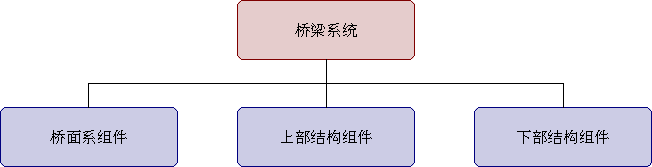
\includegraphics{bridge-system.pdf}
  % \caption{Bridge system composition}
  \caption{桥梁\gls*{system}的组成}
  \label{fig:bridge-system-composition}
\end{figure}

% As shown in \cref{fig:bridge-system-composition}, a bridge system is initially broken down into three main components: deck, superstructure and substructure. These are the primary categories or groupings of subsystems and elements within a bridge that define specific purpose and function.
如\cref{fig:bridge-system-composition} 所示,桥梁\gls*{system}最初分为三个主要部分:桥面系、上部结构和下部结构。 这些是定义特定目的和功能的桥梁\gls*{subsystem}和\gls*{element}的主要类别或分组。

% The deck component supports and receives live load and must provide a safe, smooth riding surface for traffic. It transfers live load and deck dead load to other components, which in most cases is to the superstructure. The superstructure component supports the deck and transmits loads across the span(s) to the bridge supports.
桥面系\gls*{component}支撑和承受活荷载,必须为交通提供安全、平稳的行驶表面。它将活载和桥面系恒载传递给其他\gls*{component},在大多数情况下是传递给上部结构。 上部结构\gls*{component}支撑桥面系并将各跨的荷载传递到桥梁支撑。

% The substructure component includes all elements that support the uperstructure. It transfers vertical and horizontal loads from the superstructure to the foundation material, such as soil or rock. At abutments, additional vertical and horizontal loads applied from the roadway embankment are also resisted.
下部结构\gls*{component}包括支持上部结构的所有\gls*{element}。 它将垂直和水平载荷从上部结构传递到基础材料(例如土壤或岩石)。 在桥台处,还可以抵抗来自车行道路堤的额外垂直和水平荷载。

% Often bridge systems are categorized or named by the superstructure type and material. This is discussed further in Section 2.2.3.
桥梁\gls*{system}通常按上部结构的类型和材料来分类或命名。这将在\cref{subsec:superstructure-componet}中进一步讨论。

% \subsection{Deck Component}
\subsection{桥面系\glsentrytext{component}}
\label{subsec:deck-component}
% \subsubsection{Deck Elements}
\subsubsection{桥面板\gls*{element}}

\begin{figure}
  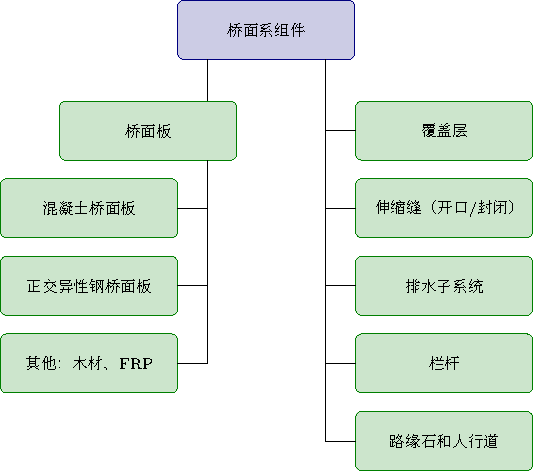
\includegraphics{component-deck.pdf}
  % \caption{Deck Componet}
  \caption{桥面系\gls*{component}}
  \label{fig:deck-component}
\end{figure}

% \cref{fig:deck-component} shows the various elements that make up the deck component, which includes the deck/slab element itself along with other related elements including overlays/wearing surfaces, expansion joints, drainage elements, railings, and curbs and sidewalks. There are various types of deck/slab elements, including concrete decks (either \acrfull{cip} or precast), steel/orthotropic decks (including open or concrete-filled steel grids), and other types including timber and FRP.
\cref{fig:deck-component} 显示了构成桥面系\gls*{component}的各种\gls*{element},其中包括桥面板\gls*{element}本身以及其他相关\gls*{element},包括覆盖层/耐磨表面、伸缩缝、排水系统\gls*{element}、栏杆和路缘石以及人行道。有多种类型的桥面板\gls*{element},包括混凝土桥面板(\acrfull{cip}或预制)、钢/正交各向异性桥面板(包括开放式或混凝土填充钢格栅)以及其他类型,包括木材和\acrfull{frp}。

% A detailed discussion of bridge decks and related service life issues is included in \cref{chp:bridge-decks}. Most decks are composite cast-in-place concrete types but other types composed of precast concrete panels (both partial depth and full depth) and posttensioning have been used, particularly with accelerated construction techniques. Steel deck types, including steel orthotropic decks, are also discussed in \cref{chp:bridge-decks}. A thorough look at materials used in bridge decks is provided in \cref{chp:materials}, and Chapter 9 examines deck expansion devices and joints.
\cref{chp:bridge-decks}中包含对桥面板\gls*{servicelife}相关问题的详细讨论。 大多数桥面板是组合现浇混凝土类型,但也使用了由预制混凝土面板(部分深度和全深度)和后张法组成的其他类型,特别是当采用\acrfull{abc}技术时。\cref{chp:bridge-decks} 中还讨论了钢桥面板类型,包括钢正交各向异性桥面板。\cref{chp:materials} 中提供了对桥面系中使用的材料的全面了解,\cref{chp:expansion-devices}梳理了桥面板伸缩装置和接缝。

% \subsubsection{Bridge Deck Drainage}
\subsubsection{桥面系排水}
% The deck drainage subsystem includes inlets or scuppers, pipes and downspouts, and outlets. The main requirement of this subsystem is to remove rainfall-generated runoff from the bridge deck before it collects and spreads excessively in the gutter to encroach onto the traveled roadway. The deck drainage subsystem must be designed to deter flow and accompanying corrosive deicing chemicals from contacting vulnerable structural members. Proper maintenance of deck drainage elements is essential to avoid clogging and malfunction and such maintenance requirements must be considered in the design.
桥面系排水\gls*{subsystem}包括集水口或泄水孔、管道和落水管以及出水口。该\gls*{subsystem}的主要作用是将降雨产生的径流从桥面收集,并于其在排水沟中过度扩散并侵占行车道之前将其从桥面板中排除。 桥面系排水\gls*{subsystem}的设计必须能够阻止水流和伴随其的腐蚀性除冰盐等化学品接触脆弱的结构构件。恰当的维护桥面系排水\gls{element}对于避免堵塞和故障至关重要,并且在设计中必须考虑此类维护要求。

% Open expansion joint drainage includes collection troughs, pipes, and attachments below open expansion joints such as tooth or sliding plate dams to collect drainage, debris, and deicing chemicals that flow through the openings and protect adjacent structural elements. Again, proper maintenance is essential and must be factored into the design.
开放式伸缩缝排水包括收集槽、管道和开放式伸缩缝下方的附件,例如齿板或滑板,用于收集流经开口的排水、杂物和除冰化学品,并保护相邻的结构\gls*{element}。同样,恰当的维护是必不可少的,必须将其纳入设计中。

% \subsubsection{Bridge Railings}
\subsubsection{桥梁护栏}
% Materials used in bridge railing designs include metal, reinforced concrete, and various combinations. Crash testing requirements have been established by FHWA and AASHTO specifications to provide adequate strength depending on vehicle size and speed. Three general categories of bridge railings are typically considered: traffic railings, pedestrian or bicycle railings, and combination railings.
桥梁护栏设计中使用的材料包括金属、钢筋混凝土和各种组合材料。 \gls*{fhwa} 和 \gls*{aashto} 规范制定了碰撞测试要求,以根据车辆尺寸和速度提供足够的强度。通常考虑三种一般类别的桥梁护栏:车行护栏、行人或自行车护栏以及组合护栏。

% \begin{itemize}
  % \item Traffic railings are designed to contain and safely redirect vehicles.
  % \item Pedestrian or bicycle railings are generally located on the outside edge of a bridge sidewalk, and are designed to safely contain pedestrians or bicyclists. AASHTO specifications require certain heights and limit the opening sizes between members.
  % \item Combination railings are dual purpose railings designed to contain both vehicles and pedestrians or bicyclists, and are generally located at the outside edge of a bridge sidewalk. With this type of railing, there is usually no other barrier between the roadway and sidewalk.
% \end{itemize}
\begin{itemize}
  \item 交通栏杆旨在控制车辆并安全地重定向车辆。
  \item 行人或自行车栏杆通常位于桥人行道的外侧边缘,旨在安全地控制行人或骑自行车的人。 \acrshort*{aashto} 规范要求一定的高度并限制构件之间的开口尺寸。
  \item 组合栏杆是双重用途的栏杆,设计用于同时控制车辆和行人或骑自行车的人,通常位于桥梁人行道的外侧边缘。 使用这种类型的栏杆,车行道和人行道之间通常没有其他护栏。
\end{itemize}

% Bridge railings are often located in high splash zones and are often subject to harsh environments that effect steel element corrosion, concrete deterioration and reinforcing bar corrosion. Special protection is necessary for long-term service life of these elements.
桥梁栏杆通常位于高飞溅区域,并且经常受到影响钢\gls*{element}腐蚀、混凝土\gls*{deterioration}和钢筋腐蚀的恶劣环境。 这些\gls*{element}的长期\gls*{servicelife}需要特殊保护。

% Bridge rails are usually cast, following the deck casting. In these instances, special attention should be paid to the cold joint that will be created between deck and cast-in-place rail as it provides a natural path for ingress of moisture and causes corrosion of reinforcement.
桥梁栏杆通常在桥面板浇筑之后进行。 在这些情况下,应特别注意将在桥面板和现浇栏杆之间形成的冷接缝,因为它提供了水分进入的自然路径并导致钢筋腐蚀。

% \subsubsection{Curbs and sidewalks}
\subsubsection{路缘石和人行道}
% Curbs and sidewalks are affected similarly to deck slabs. Information relative to these elements is provided in \cref{chp:bridge-decks} on bridge decks and \cref{chp:materials} on materials.
路缘石和人行道所受到的影响与桥面板较为相似。有关这些\gls*{element}的信息将在\cref{chp:bridge-decks}\nameref{chp:bridge-decks}和\cref{chp:materials}\nameref{chp:materials}中提供。

% \subsection{Superstructure Component}
\subsection{上部结构\glsentrytext{component}}
\label{subsec:superstructure-componet}

% The superstructure component includes the structural subsystem and bearings. A detailed discussion of bearing elements is given in Chapter 10.
上部结构部件包括结构\gls*{subsystem}和支座。\cref{chp:bridge-bearings}详细讨论了支座\gls*{element}。

\begin{figure}
  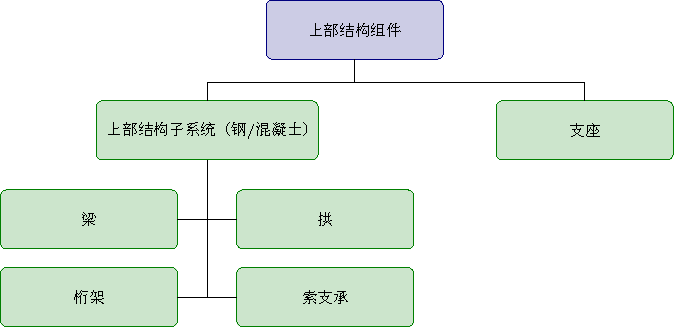
\includegraphics{component-superstructure.pdf}
  % \caption{Superstructure component}
  \caption{上部结构\gls*{component}}
  \label{fig:superstructure-component}
\end{figure}

% Superstructures are often categorized by:
上部结构通常按以下方式分类:
% \begin{itemize}
  % \item Material type. Steel or concrete are most commonly used.
  % \item Structure subsystem type. Girder subsystems are most often used for common-span lengths within the 300 feet limit. Longer spans typically use girders, trusses, arches or cable-supported types, depending on span length.
  % \item Superstructure continuity. Many older bridges were simple spans, while bridges that are more modern are fully continuous or continuous for live load. The continuous spans provide structural continuity that helps distribute traffic loads in case of excessive deterioration of some of the bridge elements. Structural continuity is especially important in instances of bridges with fracture critical elements.
  % \item Jointless Systems. Integral abutment construction is gaining popularity among many states. Integral pier construction is used only occasionally. Additional information on integral construction is provided in Chapter 8 on jointless bridges.
  % \item Modular Construction. Modular systems using prefabricated superstructure elements such as “topped girders” or preconstructed spans are becoming more popular in instances requiring accelerated construction. Durability of connection details is a concern for long-term service life of these systems. These types of connections are addressed in Chapter 8on jointless bridges.
% \end{itemize}
\begin{itemize}
  \item 材料类型。最常用的是钢材或混凝土。
  \item 结构\gls*{subsystem}类型。 梁\gls*{subsystem}最常用于 \qty{90}{m} 以内的一般跨度。更大的跨度通常使用梁、桁架、拱或缆索支承类型,这具体取决于跨度长度。
  \item 上部结构的连续性。许多老的桥梁采用简支结构,而更现代的桥梁采用完全连续或对活荷载连续的结构。连续跨提供结构连续性,有助于在某些桥梁\gls*{element}过度\gls*{deterioration}的情况下重分配交通荷载。 结构连续性在具有断裂临界\gls*{element}的桥梁实例中尤为重要。
  \item 无缝系统。整体式桥台建设在许多州越来越受欢迎。整体式桥墩施工只是偶尔使用。 关于整体结构的更多信息在\cref{chp:jointless-bridge}\nameref{chp:jointless-bridge}中给出。
  \item 模块化建造。使用“预顶梁”或预制跨等预制上部结构\gls*{element}的模块化系统在需要\acrlong*{abc}的情况下变得越来越流行。 细部连接构造的耐久性是这些系统长期\gls*{servicelife}的一个问题。 这些类型的连接在\cref{chp:jointless-bridge}\nameref{chp:jointless-bridge}中进行了介绍。
\end{itemize}

% These categories are often combined in an overall classification of the superstructure, which is frequently used to define the entire bridge system.
这些类别通常结合在上部结构的总体分类中,经常用于定义整个桥梁\gls*{system}。

% Following is a brief discussion of the most common steel and concrete superstructure types.
以下是对最常见的钢和混凝土上部结构类型的简要讨论。

% \subsubsection{Steel Superstructures}
\subsubsection{上部钢结构}
% \paragraph{Steel Girder Superstructures} 
\paragraph{钢梁上部结构} 
% The most common steel bridge superstructures today are composite multi-girder subsystems that use either rolled beams, plate girders or tub girders. These systems can be single or multi span, and can be either straight or curved. Either of these can also be skewed. Rolled beam superstructures using W-shapes are used in shorter spans up to about 100 ft for simple spans and up to about 120 ft for continuous spans. Recently, deeper rolled shapes (44 in.) for bridge applications have become available. When combined with the simple for dead and continuous for live load concept, these W-shapes can be used for longer spans. Welded plate girders are usually used for spans over 120 ft \cite{nsba2008}. \cref{fig:typical-steel-girder-superstructures} shows typical steel I-girder and tub girder systems. Recently, folded plate beam sections have been developed for short span applications. See \ref{par:steel-modular-system} for steel modular systems.
当今最常见的钢桥上部结构是使用轧制梁、板梁或小箱梁的复合多梁子系统。这些系统可以是单跨或多跨,可以是直的也可以是弯的。这些类型中的任何一种也都可以斜交布置。使用 W 形的轧制梁上部结构用于较短的跨度,简支跨度可达约 \qty{30}{m},连续跨度可达约 \qty{35}{m}。最近,更深轧制形状(\qty{1.10}{m})也已经可以用于桥梁结构中。 当与\gls{sdcl}概念相结合时,这些 W 形可使用更大的跨度。焊接板梁通常用于 \qty{35}{m}以上的跨度\cite{nsba2008}。 \cref{fig:typical-steel-girder-superstructures} 显示了典型的钢工字梁和小箱梁系统。最近,折板梁截面已被开发用于短跨度应用,可参阅 \ref{par:steel-modular-system} 了解钢制模块化系统。

\begin{figure}
  \begin{minipage}{0.48\linewidth}\centering
    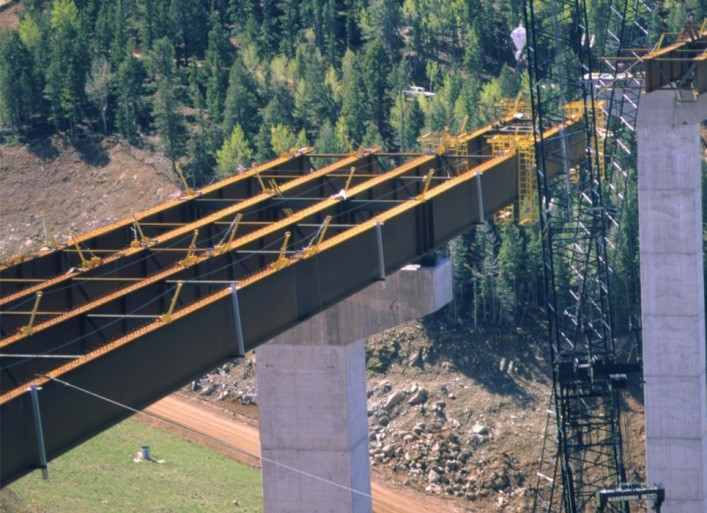
\includegraphics[height=5cm]{I-girder.jpg}
    % \subcaption{Deck I-girder system. (Courtesy HDR)}
    \subcaption{工字梁}
  \end{minipage}\hfill
  \begin{minipage}{0.48\linewidth}\centering
    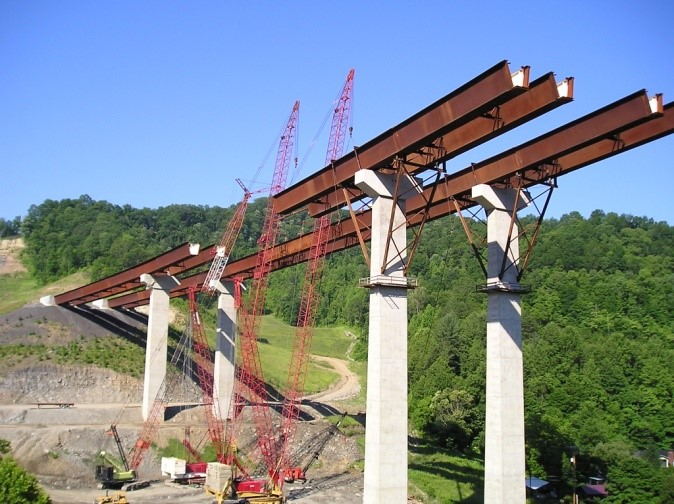
\includegraphics[height=5cm]{Tub-girder.jpg}
    % \subcaption{Tube girder system. (Courtesy Palmer Engineering)}
    \subcaption{小箱梁}
  \end{minipage}
  % \caption{Typical steel girder superstructures}
  \caption{典型钢梁上部结构}
  \label{fig:typical-steel-girder-superstructures}
\end{figure}

% Up until the 1970s, many bridges were designed with systems using two main deck girders, combined with transverse floor beams and longitudinal stringers. The perceived notion that two girder systems are not redundant led to a significant decrease in their use within the United States. However, two girder systems are very popular in Europe. Multi-girder bridges with inherent redundancy are currently preferred by many bridge owners (NSBA 2008). Use of high performance steels with greater fracture toughness, however, has led to re-evaluation of two-girder systems. Further, a memo dated June 20, 2012 by FHWA has paved the way to more use of two girder systems (FHWA 2012).
直到 20 世纪 70 年代,许多桥梁的设计系统都使用两个主纵梁,结合横梁和纵向小纵梁。 双主梁体系结构的冗余度不大,这样的观念导致它们在美国的使用很少,然而,双主梁体系在欧洲非常流行。在美国,具有固有冗余的多梁体系桥目前受到许多桥梁业主的青睐 \cite{nsba2008}。然而,在具有更高断裂韧性的高性能钢得到广泛应用后,人们对双主梁体系进行了重新评估。此外,\gls*{fhwa} 于 2012 年 6 月 20 日发布的一份备忘录为更多地使用双主梁体系铺平了道路\cite{fhwa2012a}。

% A variation to the typical multi-girder system is the girder-substringer system, which has been used as an economical concept for longer spans beyond approximately 275 ft. This system uses several heavy girders with wide girder spacing and rolled-beam stringers supported midway between the main girders by truss K-type cross frames.
典型的多梁体系的一个变体是主梁—子纵梁体系,它在被用于超过大约 \qty{83}{m} 的更大跨度时更为经济。该体系使用几个具有较大间距的重型主梁和中间支撑的轧制纵梁,主梁间采用桁架 K 型交叉框架作为横向联系。

% \paragraph{Continuity in Steel Systems}
\paragraph{钢结构体系中的连续性}

% For many years, bridges were designed as a series of simple spans with expansion joints at each pier because they were easy to design and construct. Leaking joints, however, became a leading cause of structural deterioration and the desire to eliminate joints became prevalent. Multi-span steel girder systems were also shown to be much more efficient when designed as continuous systems, making continuous design more commonplace.
多年来,桥梁被设计成一系列简支跨,每个桥墩都设有伸缩缝,因为它们易于设计和建造。 然而,当接缝缝的漏水成为结构\gls*{deterioration}的主要原因,消除接缝的愿望也就变得更普遍。当设计为连续系统时,多跨度钢梁体系也被证明效率更高,从而使连续设计更加普遍。

% Multi-span systems have typically been fully continuous for both dead load and live load, but new systems, typically with spans up to about 150 ft, have been introduced with a Simple for Dead Load and Continuous for Live Load (SDCL) concept. These systems combine the advantage of simple-span construction with the efficiency of live load continuity and the durability of not having joints that can ultimately leak.
多跨体系通常对于恒载和活载都是完全连续的,但是通常在跨度达到 \qty{45}{m} 的新体系中已经引入了\gls{sdcl}概念。 这些系统结合了简支跨建造的优势、活荷载连续性的效率以及没有最终可能漏水的接头的耐用性。

% Recently, extensive research studies have been carried out to develop practical details for SDCL steel bridge systems (Azizinamini et al. 2003, Azizinamini et al. 2005a, Azizinamini et al. 2005b; Azizinamini 2013; Lampe et al.2013; Farimani et al. 2013; Yakel and Azizinamini 2013; Javidi et al. 2013). These studies demonstrate that for the SDCL steel bridge system, continuity for live load can be provided using steel reinforcement placed over the pier, before casting deck; however, in order to provide continuity, various girder connection details have been used in practice. \cref{fig:steel-bridge-system-SDCL} shows two different details in use. Splice plates are sometimes used for top flange connections, which are in tension. The research studies previously referenced, however, do not recommend use of such detail. Bottom flanges in compression are typically butted with plates and wedges.
最近,在开发 \gls*{sdcl} 钢桥系统的实用细部构造方面已经开展了广泛的研究 \cite{azizinamini2003t,azizinamini2005d1,azizinamini2005d2,azizinamini2014s,lampe2013d,farimani2014n,yakel2014f,javidi2013e} 。这些研究表明,对于 \gls*{sdcl} 钢桥系统,在浇筑桥面之前,可以使用在墩顶设置的钢筋来提供活荷载的连续性;然而,为了提供连续性,在实践中使用了各种梁连接构造。\cref{fig:steel-bridge-system-SDCL} 显示了两个不同的细部构造:顶部受拉翼缘板有时用拼接板连接,然而,先前引用的研究不建议使用此类构造;底部受压的翼缘板通常采用板和楔子顶紧。

% The disadvantage of the continuity detail with the top flange splice is that the bolts for connecting the top plate have to be tightened after casting the deck. This creates additional construction sequencing with a separate closure pour over the pier.
顶部受拉翼缘板拼接的连续构造的缺点是在浇铸桥面板后必须拧紧用于连接顶板的螺栓。 这会创建额外的施工顺序,并在桥墩上单独浇筑。

\begin{figure}
  \begin{minipage}{0.48\linewidth}\centering
    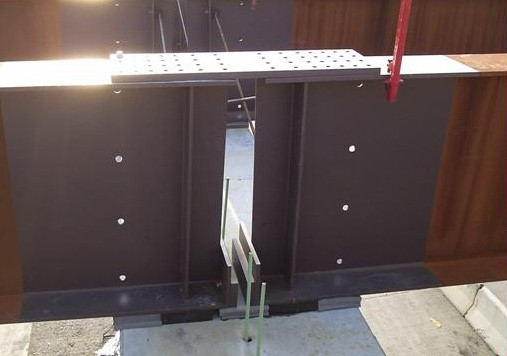
\includegraphics[height=5cm]{cont-with-top-flange-splice.jpg}
    \subcaption{顶部翼缘板带有拼接的桥面连续}
  \end{minipage}\hfill
  \begin{minipage}{0.48\linewidth}\centering
    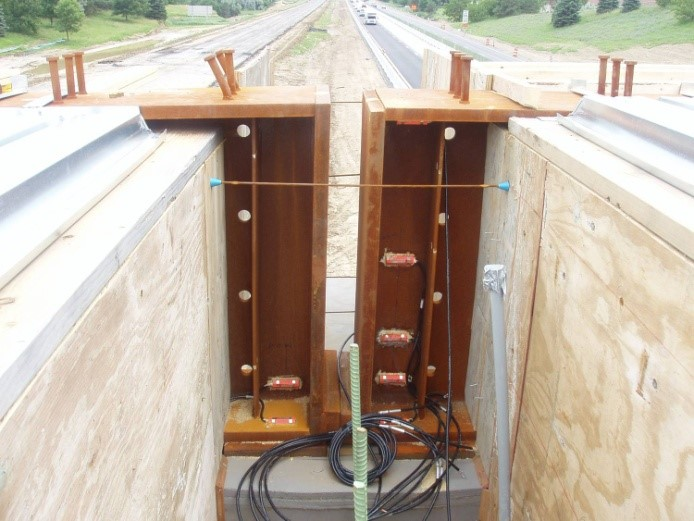
\includegraphics[height=5cm]{cont-without-top-flange-splice.jpg}
    \subcaption{顶部翼缘板不带拼接的桥面连续}
  \end{minipage}
  \caption{\acrshort*{sdcl}概念的钢桥}\label{fig:steel-bridge-system-SDCL}
\end{figure}

% \paragraph{Long-Span Superstructures}
\paragraph{大跨度上部结构}

% \cref{fig:long-span-steel-bridge-superstructures} shows examples of long-span girder, truss, arch, and cable-stayed bridge systems. Steel plate girder systems have been used for spans up to approximately 500 ft. Spans up to 400 ft have been designed economically with parallel flanges. Variable-depth haunched girders have been used in the 350-ft to 500-ft range. Use of highperformance steel (HPS 70W) has shown economy for plate girder and tub girder systems in most span ranges over 150 ft, particularly in hybrid combinations. Studies have shown that hybrid configurations using conventional grade 50W steel in webs and HPS 70W steel in top and bottom flanges in negative moment regions and bottom flanges in positive moment regions are typically the most economical (Horton et al. 2002). Top flanges in positive moment regions are affected by composite action with the deck and cannot realize enough benefit from the use of higherstrength steel to be economical, except for longer spans. Use of HPS 70W steel in long-span negative moment ranges can also permit economical parallel flange design without expensive haunches. Trusses, arches, cable-stayed, and suspension systems have also been used for longer-span applications, typically over 500 feet. For spans up to 300 feet, deck girder systems are the most applicable.
\cref{fig:long-span-steel-bridge-superstructures} 显示了大跨度梁、桁架、拱和斜拉桥体系的示例。钢板梁体系已用于高达约 \qty{150}{m} 的跨度。\qty{120}{m} 的跨度已被设计为具有平行翼缘板的经济型。 在 \qtyrange{105}{150}{m} 的范围内使用了变高度的加腋梁。在超过 \qty{45}{m} 的大多数跨度范围内,特别是在不同钢种的混合配置中,高性能钢(HPS 70W)的使用已经显示出钢板梁和钢小箱梁系统的经济性。研究表明,在腹板中使用传统等级 50W 钢,在负弯矩区域的顶底部翼缘板和正弯矩区域底部翼缘板中使用 HPS 70W 钢,这种混合配置通常是最经济的 \cite{horton2003h}。正弯矩区域的顶部翼缘受到与桥面板的联合作用的影响,并且不能从使用高强度钢中获得足够的好处以达到经济的目的,除非是更长的跨度。在大跨度负弯矩范围内使用 HPS 70W 钢还可以实现经济的平行翼缘板设计,而无需昂贵的腰部。 桁架、拱、斜拉索和悬吊系统也已用于较长跨度的应用,通常超过 \qty{150}{m}。 对于 \qty{90}{m} 以内的跨度,钢板梁系统是最适用的。

\begin{figure}
  \begin{minipage}{0.48\linewidth}\centering
    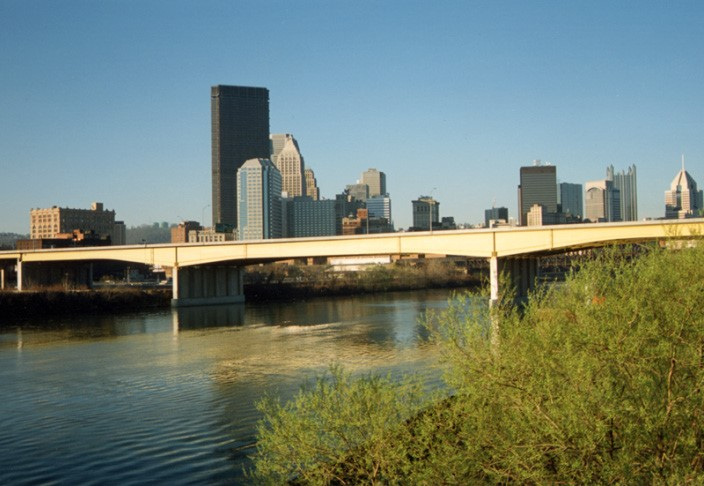
\includegraphics[height=5cm]{long-span-plate-girder.jpg}
    \subcaption{大跨度板梁}
  \end{minipage}\hfill
  \begin{minipage}{0.48\linewidth}\centering
    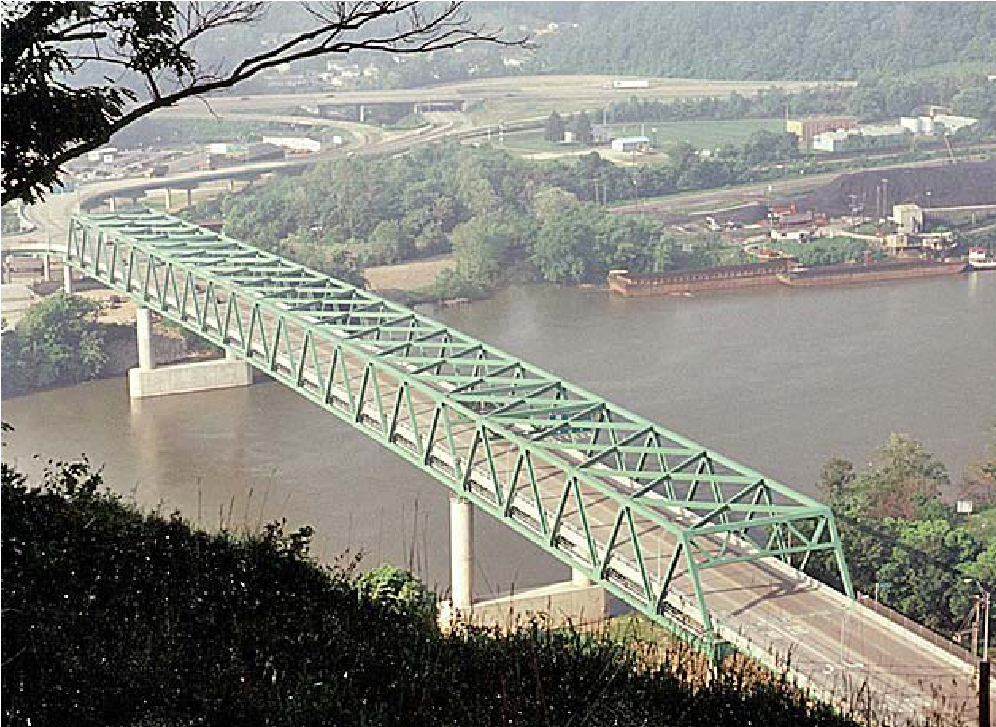
\includegraphics[height=5cm]{continuous-truss.png}
    \subcaption{连续桁架}
  \end{minipage}
  \begin{minipage}{0.46\linewidth}\centering
    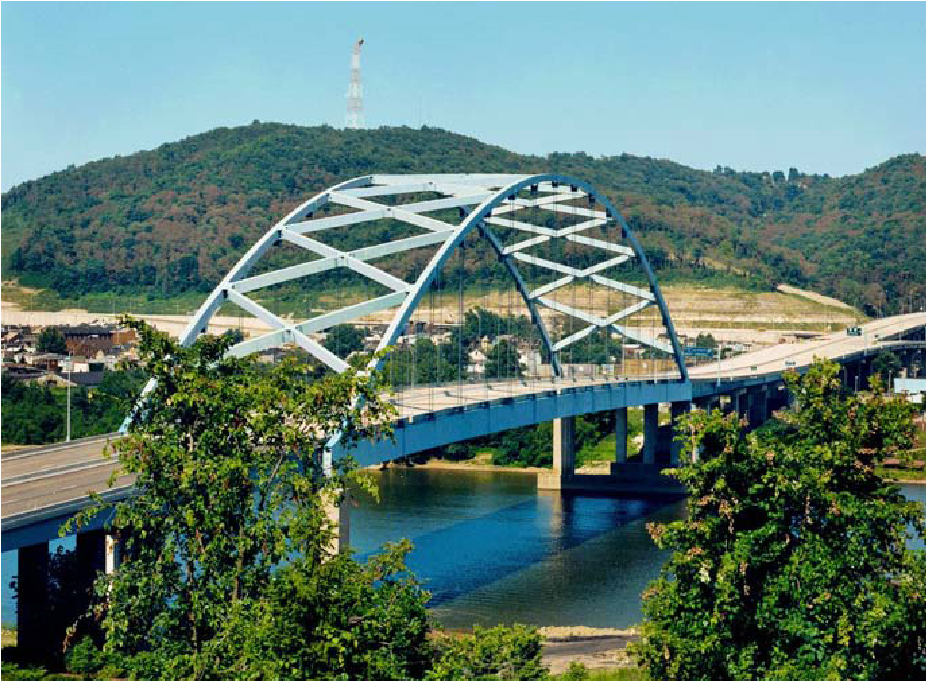
\includegraphics[height=5cm]{tied-arch.png}
    \subcaption{系杆拱}
  \end{minipage}\hfill
  \begin{minipage}{0.52\linewidth}\centering
    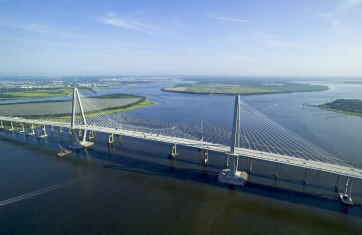
\includegraphics[height=5cm]{cable-supported.jpg}
    \subcaption{索支承桥梁}
  \end{minipage}
  % \caption{Long-span steel bridge superstructures. (All Figures Courtesy HDR)}
  \caption{大跨度钢桥上部结构}
  \label{fig:long-span-steel-bridge-superstructures}
\end{figure}

% Long-span structures can have special needs for addressing long-term service life relating to unique details, inspection, and maintenance. Access for inspection and maintenance can require elaborate systems of inspection walkways and access ladders, particularly for access to fracture-critical members. Older trusses typically require heavy maintenance because of large surface area to weight ratio, and riveted, built-up members with lacing bars subject to pack-out and other surface corrosion. Truss joint details typically have moisture and debris traps that initiate corrosion, while newer trusses have cleaner surface details that are more easily painted and maintained.
大跨度结构在解决与独特细节、检查和维护相关的长期使用寿命方面可能有特殊需求。 检查和维护通道可能需要精心设计的检查走道和通道梯系统,特别是对于断裂关键部件的通道。较旧的桁架通常需要大量维护,因为它的表面积与重量比很大,并且带有拉筋的铆接组合构件容易被压裂和其他表面腐蚀。桁架接头细节通常有湿气和杂物陷阱,会引发腐蚀,而较新的桁架有更清洁的表面细节,更容易涂漆和维护。

% Through structures are subject to splash zone wetting environments for all structural elements near roadway edges. This needs to be considered in a corrosion protection and maintenance plan. Long-span bridges have large thermal movement requirements that result in large expansion joints. This requires even additional attention to joint maintenance to prevent deck drainage from spilling through. Heavy loads and large thermal movements also require special bearing designs. Navigation channel crossings are subject to vessel collision and need to be protected.
对于靠近道路边缘的所有结构\gls*{element},贯通结构都受到飞溅区润湿环境的影响。这需要在腐蚀保护和维护计划中加以考虑。大跨度桥梁具有较大的温度作用变形要求,因此会需要较大的伸缩缝。 这甚至需要额外注意接头维护,以防止桥面板排水系统溢出。 重载荷和大的温度作用变形也需要特殊的支座设计。 航道交叉口容易受到船只碰撞,需要加以保护。

% \paragraph{Steel Modular Systems}
\paragraph{钢结构模块化系统}
\label{par:steel-modular-system}

% New steel systems that provide for accelerated construction include modular construction with pre-topped deck. Modular orthotropic deck systems are also a consideration. These modular systems require special attention to both transverse and longitudinal connection details for achieving long-term durability.
提供快速建造的新钢系统包括带有预顶板的模块化结构。 模块化正交各向异性桥面板系统也是一个考虑因素。 这些模块化系统需要特别注意横向和纵向连接构造,以实现长期耐用性。

% Pre-top modular bridge systems are best suited for accelerated bridge construction applications. In these systems, several units consisting of pre-topped steel or concrete girders are placed side by side and joined together using longitudinal closure pours. The service life of these pre-topped modular systems is significantly influenced by service life of longitudinal closure pour. Pre-topped steel modular systems present two major advantages:
预顶模块化桥梁系统最适合\acrlong*{abc}应用。 在这些系统中,几个由预顶钢或混凝土梁组成的单元并排放置,并使用纵向闭合浇注连接在一起。 这些预先加盖的模块化系统的{使用寿命}受纵向封闭浇注的{使用寿命}的显着影响。 预盖钢模块化系统具有两大优势:

% \begin{enumerate}
%   \item The use of steel girders significantly reduces the creep and shrinkage deflections.
%   \item Pre-topped steel modular units weigh less.
% \end{enumerate}
\begin{enumerate}
  \item 钢梁的使用显着降低了蠕变和收缩挠度。
  \item 预顶的钢结构模块化单元重量更轻。
\end{enumerate}

% The Folded Plate Bridge System is a new modular system that offers an economical solution for many short-span bridge applications. The system consists of a series of standard shapes that are built by bending flat plates into inverted tub sections using a press break, as shown in \cref{fig:making-of-folded-plate-girder-using-break-press}.
折叠板桥系统是一种新型模块化系统,可为许多短跨度桥梁应用提供经济的解决方案。 该系统由一系列标准形状组成,这些标准形状是通过使用压力折断将平板弯曲成倒置的桶形部分而构建的,如 \cref{fig:making-of-folded-plate-girder-using-break-press} 所示。

\begin{figure}
  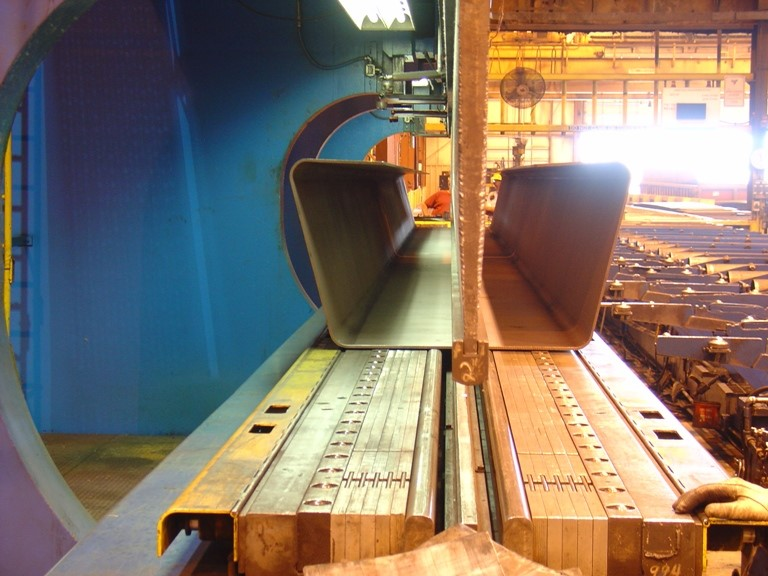
\includegraphics[width=0.7\linewidth]{folded-plate.jpg}
  % \caption{Making of folded plate girder using break press. (Courtesy UNL)}
  \caption{使用断裂压力机制作折叠板梁(由 \acrshort{unl} 提供)}
  \label{fig:making-of-folded-plate-girder-using-break-press}
\end{figure}

% The maximum span length for this system is currently limited to about 60 feet, reflecting the longest press breaks available in the industry.
该系统的最大跨度长度目前限制在 60 英尺左右,反映了行业中可用的最长压力中断。

% The process of bending the girder can take less than an hour. Geometrical variations are obtained simply by changing the bend locations. Varying the depth of the web and the width of the top and bottom flanges allow the folded plate girders to accommodate different span length requirements.
弯曲大梁的过程可能需要不到一个小时。 只需改变弯曲位置即可获得几何变化。 改变腹板的深度以及顶部和底部翼缘的宽度允许折叠板梁适应不同的跨度长度要求。

% One of the advantages of the Folded Plate Bridge System is its promise for rapid delivery. All folded plate girders are fabricated using either 0.375- or 0.5-in. thick plate. The ability to stock standard plate sizes means the girders can be produced and delivered quickly.
折叠板桥系统的优势之一是它对快速交付的承诺。 所有折叠板梁均使用 0.375 或 0.5 英寸制造。 厚板。 库存标准板尺寸的能力意味着可以快速生产和交付大梁。

% The Folded Plate Bridge System can be constructed using conventional construction techniques as well as using principles of Accelerated Bridge Construction. In the case of conventional construction procedures, readily available construction equipment can be used to build the formwork for casting the concrete deck, as shown in \cref{fig:deck-forming-conventional}.
折叠板桥系统可以使用传统的施工技术以及\acrlong{abc}的原理来建造。 在传统施工程序的情况下,现成的施工设备可用于建造用于浇注混凝土甲板的模板,如 \cref{fig:deck-forming-conventional} 所示。

\begin{figure}
    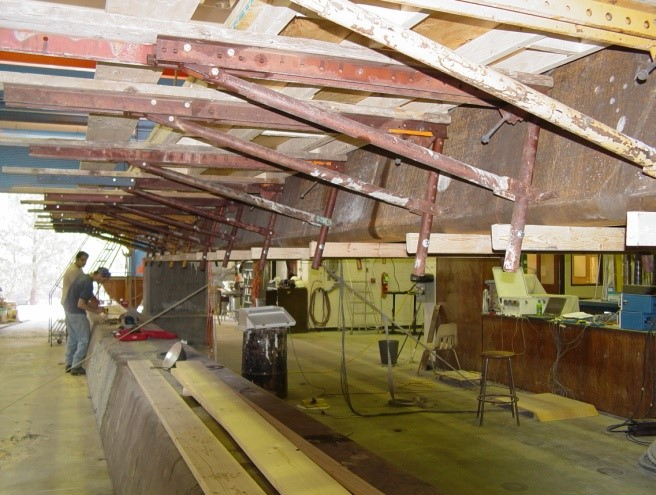
\includegraphics[height=5.5cm]{deck-forming1.jpg}\hfill
    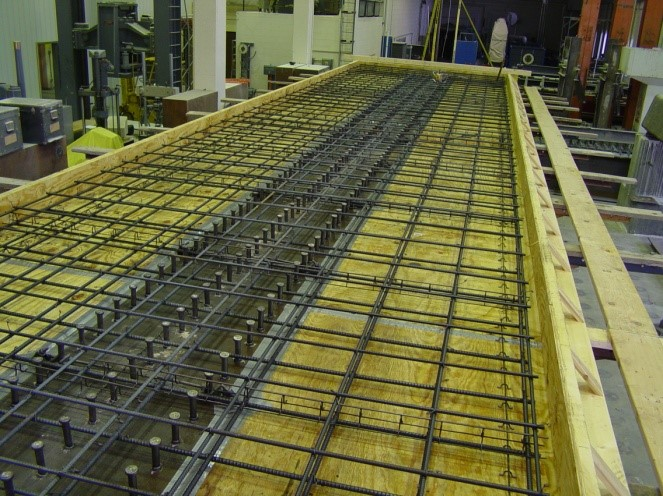
\includegraphics[height=5.5cm]{deck-forming2.jpg}
  % \caption{Deck forming using conventional approach. (Courtesy UNL)}
  \caption{使用传统方法施工桥面板(由 \acrshort{unl} 提供)}
  \label{fig:deck-forming-conventional}
\end{figure}

% Recently, the trend within the bridge construction industry has been toward reducing construction activities on the bridge site and eliminating the interruption to traffic. Therefore, an alternate and perhaps better approach when using the Folded Plate Girder System to construct short-span bridges is to use prefabricated elements.
近来,桥梁建设行业的趋势是减少桥梁现场的施工活动并消除交通中断。 因此,使用折叠板梁系统建造短跨度桥梁时,另一种可能更好的方法是使用预制构件。

% In one scenario, the tributary width of concrete deck for each folded plate girder is cast on the girder prior to shipping to the site. In this case, each prefabricated girder unit is a folded plate girder with a precast deck as shown in \cref{fig:precast-folded-plate-girder-unit}. The steel girder can be supported at the ends, or continuously supported along the length during casting, in which case all dead loads are carried by the composite section, thereby reducing deflections.
在一种情况下,每个折叠板梁的混凝土桥面板的支流宽度在运输到现场之前浇铸在梁上。 在这种情况下,每个预制梁单元都是带有预制桥面板的折叠板梁,如 \cref{fig:precast-folded-plate-girder-unit} 所示。 钢梁可以在端部支撑,也可以在浇铸过程中沿长度连续支撑,在这种情况下,所有恒载均由复合截面承载,从而减少挠度。

\begin{figure}
  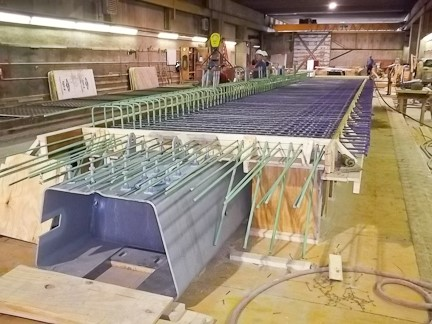
\includegraphics[height=5.5cm]{precast-unit1.jpg}\hfill
  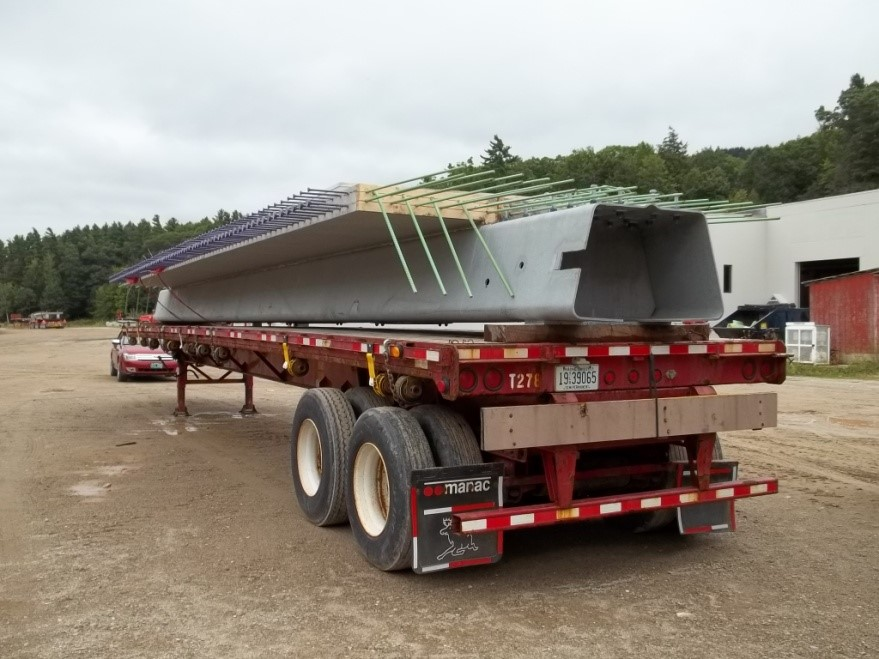
\includegraphics[height=5.5cm]{precast-unit2.jpg}
  % \caption{Precast folded plate girder unit. (Courtesy Massachusetts DOT)}
  \caption{预制折板梁单元(由马萨诸塞州\acrlong*{dot}提供)}
  \label{fig:precast-folded-plate-girder-unit}
\end{figure}

% A typical two-lane county-type bridge will require three or four prefabricated folded plate girder units placed side by side and connected longitudinally at the deck, as shown in \cref{fig:folded-plate-girder-system}. The connection between the units can be accomplished using a number of methods. A 40-ft-long folded plate girder with precast deck weighs about 24,000 pounds, allowing use of a relatively lightweight crane on the construction site.
一座典型的双车道县级桥梁将需要三个或四个预制折叠板梁单元并排放置并在桥面板上纵向连接,如\cref{fig:folded-plate-girder-system} 所示。单元之间的连接可以使用多种方法来完成。一个 \qty{12}{m} 长的带预制桥面板的折叠板梁重约 \qty{10.9}{\tonne},允许在施工现场使用相对轻便的起重机。

\begin{figure}
  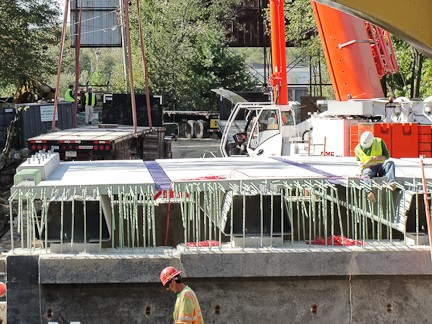
\includegraphics[height=5.5cm]{folded-plate-girder1.jpg}\hfill
  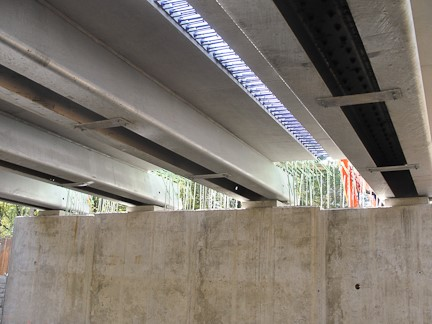
\includegraphics[height=5.5cm]{folded-plate-girder2.jpg}
  % \caption{Folded plate girder system. (Courtesy Massachusetts DOT)}
  \caption{折板梁系统(由马萨诸塞州\acrlong*{dot}提供)}
  \label{fig:folded-plate-girder-system}
\end{figure}

% \subsubsection{Concrete Bridge Superstructures}
\subsubsection{混凝土桥梁上部结构}

% There are several commonly used reinforced concrete bridge systems in the United States. The type of system implemented at a particular site is generally dictated by economics and the system's ability to accommodate the required span, or geometric requirements such as curvature.
美国有几种常用的钢筋混凝土桥梁体系。 在特定地点实施的系统类型通常由经济性和系统适应所需跨度或几何要求(如曲率)的能力决定。

% The most commonly used concrete bridge superstructures are:
最常用的混凝土桥梁上部结构有:

% \begin{itemize}
%   \item Cast-in-place concrete slabs;
%   \item Precast concrete box beams including both spread and adjacent box beams;
%   \item Precast concrete I-girders including standard I-girders, bulb-tee girders, and U-beams;
%   \item Precast concrete spliced girders, including spliced I-girders, U-beams, and box girders;
%   \item Cast-in-place posttensioned box girders;
%   \item Segmental posttensioned concrete box girders, including both precast or cast-in-place;
%   \item Concrete arches; and
%   \item Modular pre-topped concrete girder units, which are typically used for accelerated bridge construction.
% \end{itemize}
\begin{itemize}
  \item 现浇混凝土板桥;
  \item Precast concrete box beams including both spread and adjacent box beams;
  \item Precast concrete I-girders including standard I-girders, bulb-tee girders, and U-beams;
  \item Precast concrete spliced girders, including spliced I-girders, U-beams, and box girders;
  \item Cast-in-place posttensioned box girders;
  \item Segmental posttensioned concrete box girders, including both precast or cast-in-place;
  \item Concrete arches; and
  \item Modular pre-topped concrete girder units, which are typically used for accelerated bridge construction.
\end{itemize}

% \paragraph{Cast-in-Place (CIP) Concrete Slabs}
\paragraph{现浇混凝土板桥}

Full-depth, cast-in-place concrete slab superstructures consist of a concrete slab spanning between substructure units without the aid of supporting stringers, as shown in Figure 2.11. Concrete slab bridges commonly span less than 50 feet and are typically used over minor water crossings. This bridge system was traditionally constructed as a series of simple spans, but in recent years, the use of continuous spans has gained favor, eliminating the joints over the substructure units. This system is commonly reinforced conventionally, but can also be posttensioned to increase the span length range. The haunched posttensioned concrete slab system used in Kansas can span up to about 100 feet. Many states, especially in the Midwest, own many older concrete slab bridges, mainly constructed in 1930s, that have shown a very good performance history. When rated, these older concrete slab bridges usually demand posting. However, research results indicate that older concrete slab bridges possess reserve capacity significantly more than that indicated by routine rating calculations (Azizinamini et al. 1994a, 1994b). The main reason for such high capacity of older concrete slab bridges is the higher yield strength of reinforcement used versus the assumed value in rating calculations. This higher capacity of existing older concrete slab bridges coupled with their good performance record can be advantageous when developing maintenance plans.

\begin{figure}
  \begin{minipage}{0.49\linewidth}\centering
    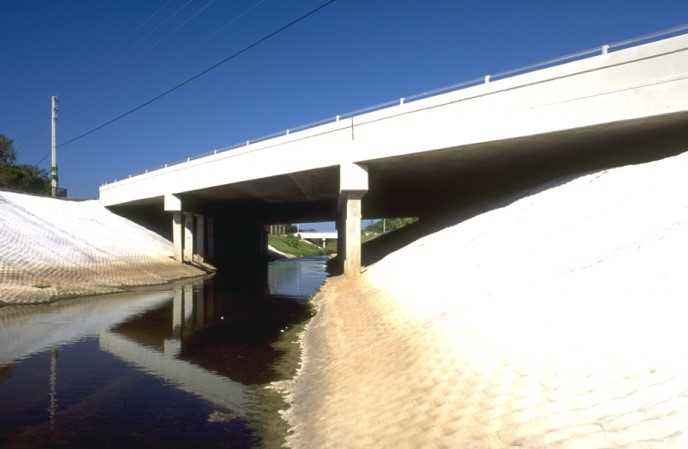
\includegraphics[height=4.8cm]{flat-slab.jpg}
    \subcaption{现浇混凝土平板桥}
  \end{minipage}\hfill
  \begin{minipage}{0.49\linewidth}\centering
    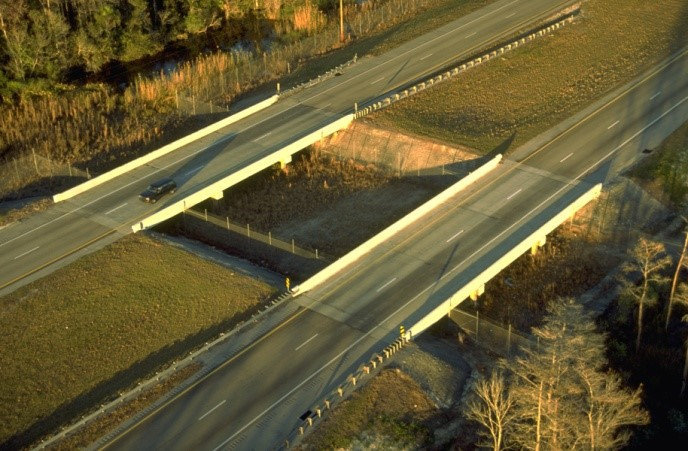
\includegraphics[height=4.8cm]{transv-post-prestress.jpg}
    \subcaption{横向后张法预应力板}
  \end{minipage}
  % \caption{Short-span concrete bridge applications. (Courtesy Atkins North America, Inc.)}
  \caption{小跨径混凝土桥梁的应用(由 Atkins North America, Inc. 友情提供)}
  \label{fig:short-span-concrete-bridge-applications}
\end{figure}

\paragraph{Precast Concrete Box Beams}

This type of superstructure consists of adjacent precast concrete box beams with non-composite deck, adjacent box beams with composite cast-in-place (CIP) concrete deck, and spread box beams with composite CIP concrete deck. Shallower precast solid and voided rectangular slabs also fall into this category. Precast concrete box beams are typically plant manufactured standard AASHTO-PCI sections that range in depth from 27 in. to 42 in. and are available in 36-in. or 48-in. widths. These precast girders are plant-produced, which generally results in high quality products.

Precast adjacent box beam bridges are the most prevalent box girder system for short and medium-span bridges, typically 20 to 127 feet, especially on secondary roadways. These bridges consist of multiple precast concrete box beams that are butted against each other to form the bridge deck and superstructure. Their advantage is that they eliminate the need for forming when using a composite CIP deck, or can be used directly with a bituminous overlay in the non-composite state. Adjacent box beams are generally connected using partial or full-depth grouted shear keys along the sides of each box. Transverse ties are usually used in addition to the grouted shear keys and may vary from a limited number of threaded rods to several posttensioned tendons. In some cases, no topping is applied to the structure while in other cases a non-composite topping or a composite structural slab is added. Problems have been encountered with adjacent non-composite box beam superstructures and are further discussed in Section 2.3.3.2.2.

\paragraph{Precast Concrete Girders}

Precast concrete I-girders with composite cast-in-place deck are commonly used concrete bridge superstructures in the 50- to 150-ft-plus span range. These girders are made of high-performance, plant-produced materials and are generally very durable and result in high quality products. In a bridge system consisting of I-girders with composite CIP slabs, commonly referred to as beam-slab bridges (see \cref{fig:concrete-I-girder-with-composite-deck}), the longitudinal stringers are often prestressed concrete I-girders using one of six standard AASHTO-PCI sections, Types I through VI, which vary in depth from 28 to 54 in. In addition, newer standard AASHTO-PCI bulb-tee (BT) shapes are used in 54-, 63-, and 72- in. depths. These standard I and BT shapes accommodate various span requirements up to about 170 ft.

Bulb-tee shapes were developed to provide increased efficiency over original I shapes. They have wide top flanges similar to Type V and VI girders that increase stability for handling and shipping and reduce deck forming. However, bulb-tees also have thinner top flanges, webs and bottom flanges that reduce weight, and have other flange geometric and proportioning modifications that optimize the sections. A number of states including Washington, Colorado, Florida and Nebraska have developed special bulb-tee shapes, modifying the standard AASHTO-PCI BT shapes, to accommodate local needs and practice.

\begin{figure}
  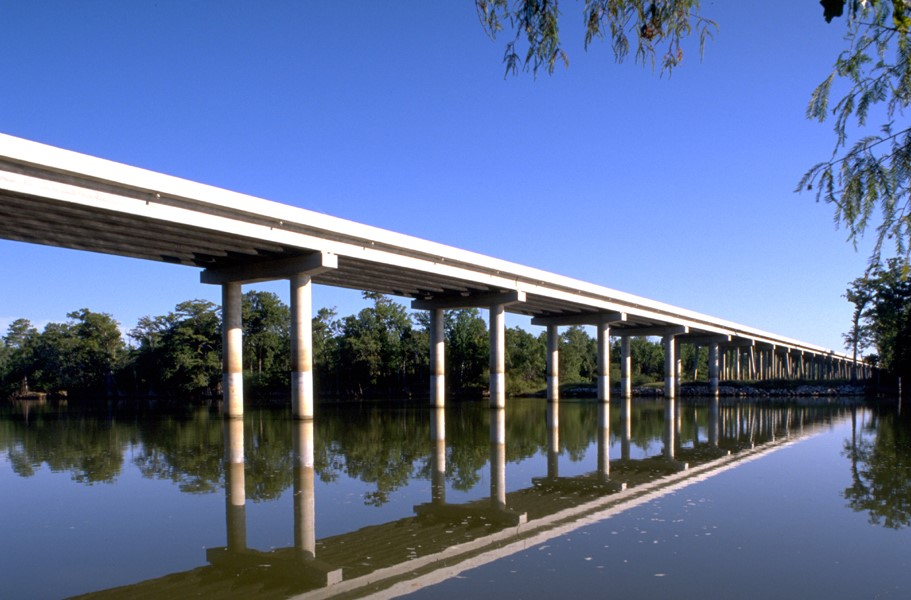
\includegraphics[width=0.8\linewidth]{concrete-I-girder-with-composite-deck.jpg}
  % \caption{Prestressed concrete I-girder bridge with composite concrete deck. (Courtesy Atkins North America, Inc.)}
  \caption{带复合混凝土桥面板的预应力混凝土工字梁桥}
  \label{fig:concrete-I-girder-with-composite-deck}
\end{figure}

A noteworthy I-girder advancement is the NU I-girder, which was developed by the University of Nebraska (UNL) in cooperation with the Nebraska Department of Roads, and has a series of eight standard shapes with depths ranging from 29.5 to 94.5 in. (Geren and Tadros 1994; Hanna et al. 2010). The NU girders have several section efficiency enhancements such as wide and thick bottom flanges that enable increased strand capacity for simple spans and provide increased negative moment capacity for continuous spans. The wide bottom flanges also provide increased stability in shipping and handling. Curved fillets in top and bottom flanges reduce stress concentration and aid the flow of concrete during fabrication. With the increased section efficiencies, these girders have been used for spans greater than \qty{60}{m} (see \cref{fig:nu-i-girder}).

\begin{figure}
  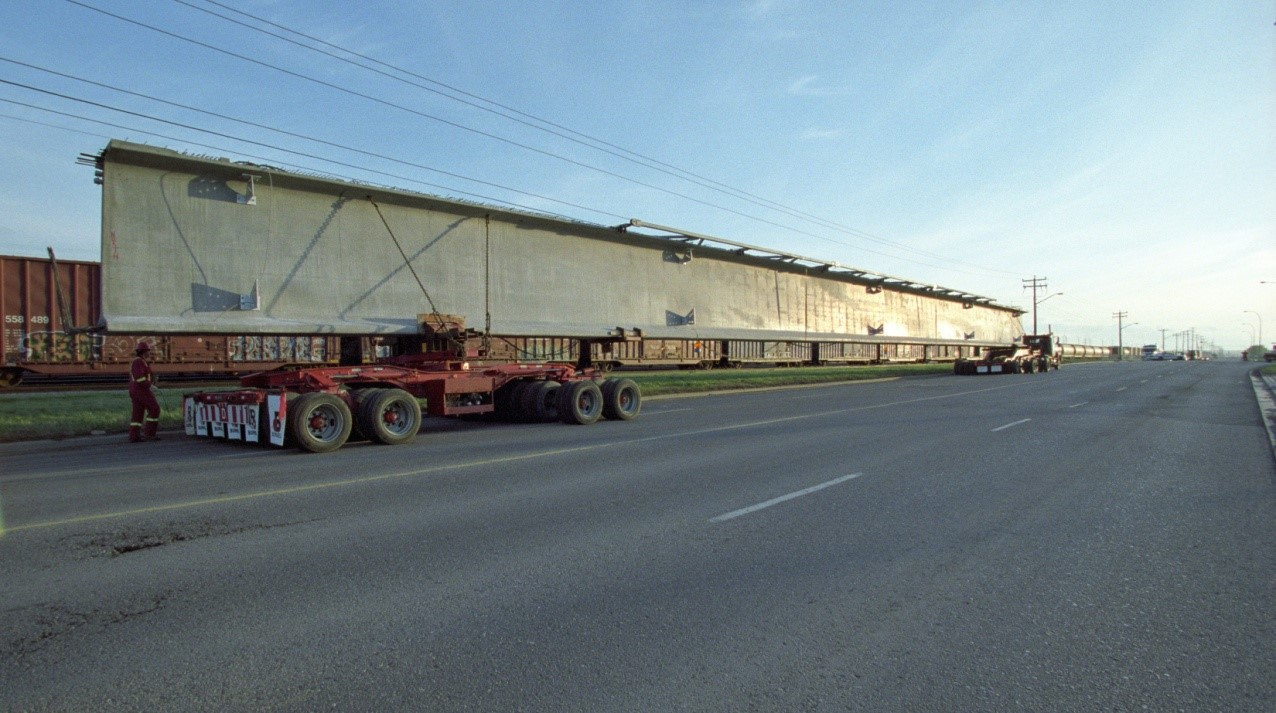
\includegraphics[width=0.9\linewidth]{nu-i-girder.jpg}
  % \caption{A 9-ft x 3-in. deep, 213-ft-long, 130-ton NU I-girder being shipped. (Courtesy of Con-Force Structures, a division of Armtec Limited Partnership, Calgary, Alberta, Canada)}
  \caption{长 \qty{65}{m}、高 \qty{2.8}{m}、重 \qty{130}{t} 的 NU I 型梁正在装运。}
  \label{fig:nu-i-girder}
\end{figure}

In many instances, precast concrete I-girders are erected as simple spans and then connected over the piers to form continuous for live load systems that eliminate deck joints.

A newer alternative to concrete I-girders is the U-beam, or concrete tub girder, concept, first developed in Texas
and now used in other states including Florida and Washington State, that provides economic and aesthetic spread
beam systems. The Texas U54 beam is 54-in. deep, similar to an AASHTO Type IV beam, and can span up to about
140 feet (Ralls et al. 1993). The Florida U-beams have four depths ranging from 48 in. to 72 in., and can be used in
spans ranging from about 100 ft to 160 ft (FDOT 2012). Washington State (WSDOT) U-beams are similar and have
four depths varying from 54 in. to 72 in., and bottom flanges that are either 4-ft or 5-ft wide. Similar to Florida, these beams can accommodate span lengths up to 160 ft. With a composite concrete deck, U- beams form a trapezoidal
box shape, similar to steel tub girders. These beams are typically designed to act as simple spans under both dead
load and live load, even when the deck is placed continuous across intermediate supports. As with I-girders, these
beams are plant produced and result in high quality products.

\paragraph{Precast Concrete Spliced Girders}
Spliced girders are precast concrete girders fabricated in several segments that are then assembled
longitudinally, typically using posttensioning, into a single simple-span or continuous girder for the final bridge
structure. They have been used to extend the span lengths of regular short- to medium-span precast concrete girders
and are designed to utilize the economy and high quality of plant-produced precast girders for longer span
applications. The length and weight of typical precast girders prevents them from being effectively used on spans
greater than about 150-feet due to the limitations of transportation equipment and available cranes. However, with
spliced girders, precast girder segments with manageable weights and lengths are transported to the construction site
and then joined together. This can either be done by splicing girder segments on the ground and erected them into
their final position, or by placing girder segments on temporary supports and then splicing them in their final
position. Spliced girders have been used for simple spans up to about 220 ft, and for continuous spans up to about
320 ft, and have been found to provide an economical concrete superstructure type in span ranges between that of
conventional precast girders and segmental box girders. \cref{fig:spliced-i-girder} shows a typical spliced girder span under
construction using temporary supports.

\begin{figure}
  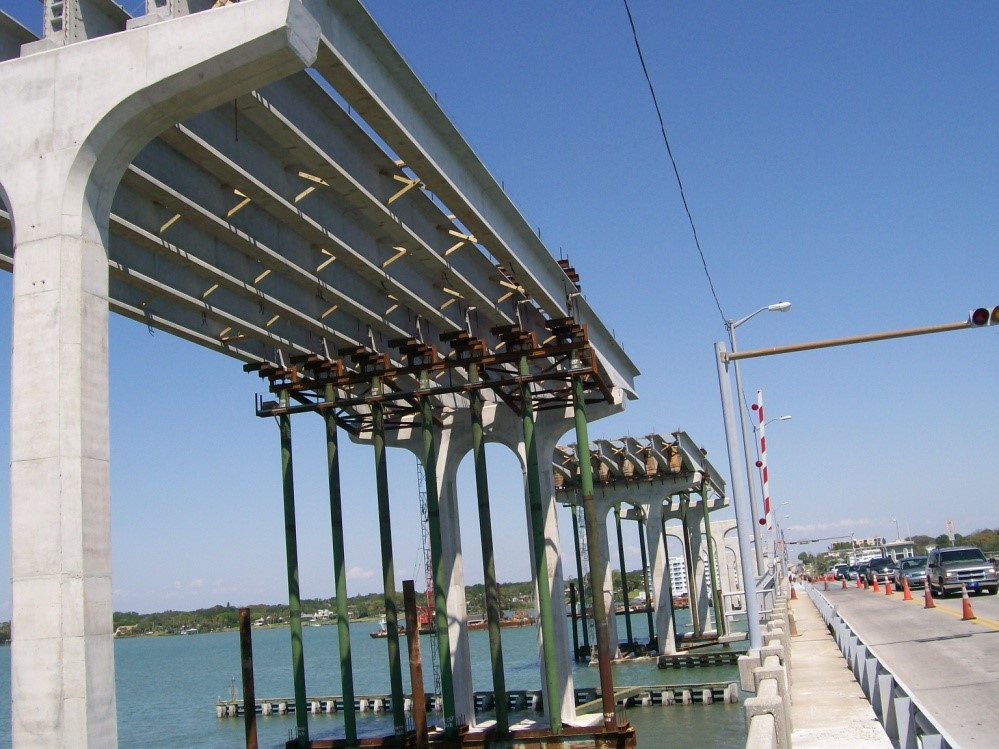
\includegraphics[width=0.65\linewidth]{spliced-i-girder.jpg}
  \caption{Spliced I-girder construction. (Courtesy HDR)}\label{fig:spliced-i-girder}
\end{figure}


Spliced girders are typically used on relatively straight alignments; however, in recent years they have also been
used for curved alignments in Nebraska and Colorado. \cref{fig:spliced-concrete-curved-box} shows a spliced-box girder bridge recently built
in Denver, Colorado.

\begin{figure}
  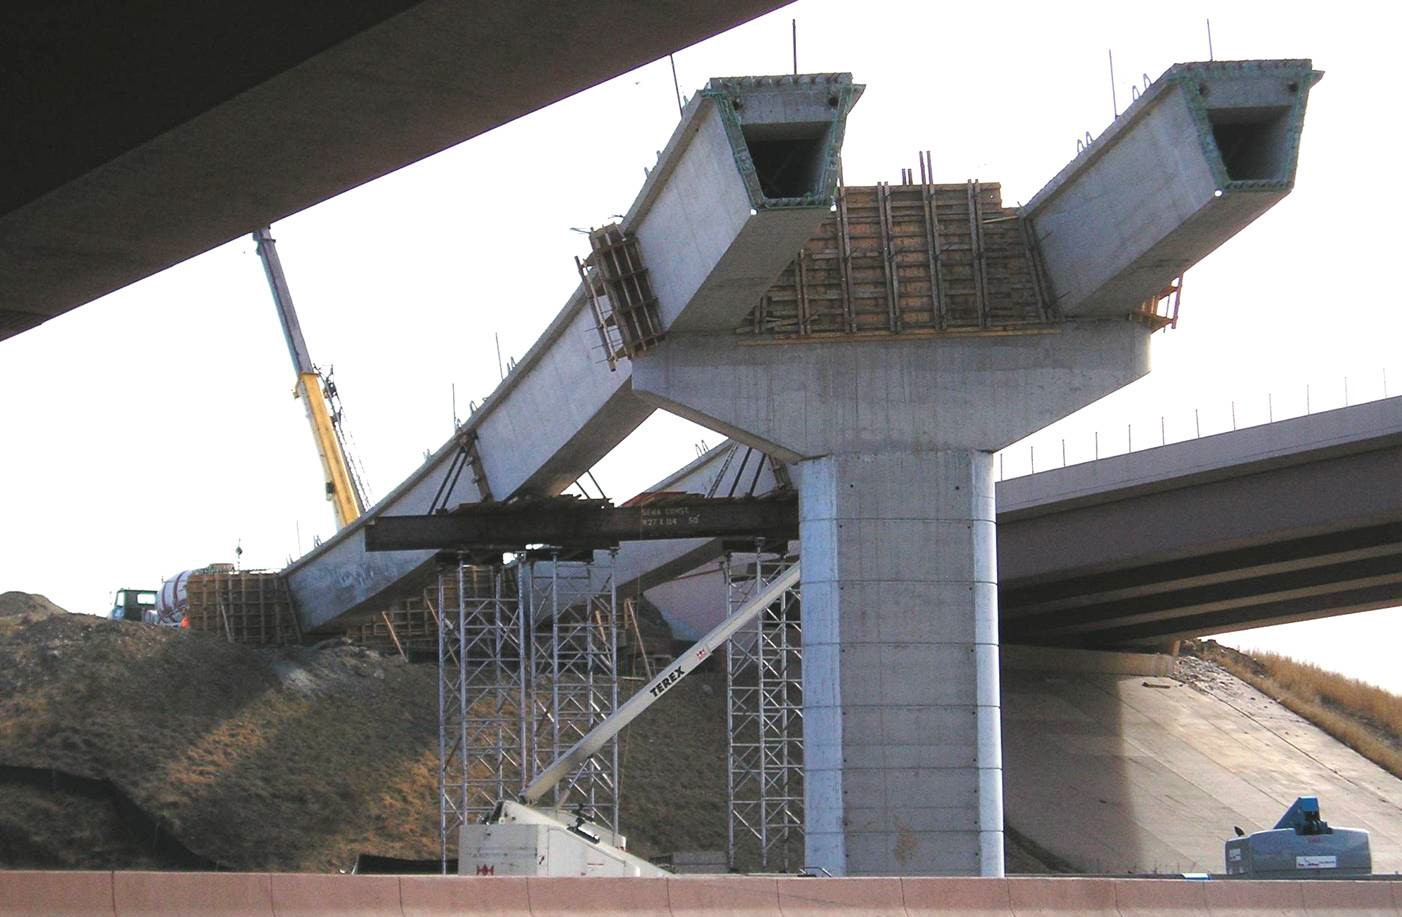
\includegraphics[width=0.65\linewidth]{spliced-concrete-curved-box.jpg}
  \caption{Spliced concrete curved boxes. (Courtesy Summit Engineering Group)}
  \label{fig:spliced-concrete-curved-box}
\end{figure}

Precast spliced girders have some similarity with segmental box girders in that both structure types consist of
smaller girder segments that are assembled and connected by posttensioning to form a final, longer girder, and both
types are erected by staged construction. However, spliced girders and segmental box girders are quite different in
the length of segments, type of splices, types of sections, tendon locations, and construction methods. Also, a
composite concrete deck is typically cast on spliced girders, while the deck slab is typically cast as an integral part of
a segmental box girder. Spliced girders use bulb-tee, I-beam, U-beam, or box shapes, while segmental box girders are
typically box shapes.



\paragraph{Cast-in-Place (CIP) Posttensioned Concrete Box Girders (on Falsework)}

Posttensioned concrete box girders cast continuously on falsework, have become very popular in several states,
particularly California, Arizona, and Nevada, and have been used in spans up to about 350 feet. This type of
construction lends itself to local construction industry practices in which contractors can economically provide the
required falsework. Similar to segmental construction, CIP on falsework offers the advantage of longer spans than
conventional girders, and can easily accommodate curved alignments. CIP construction also allows clean lines and
architectural finishes that improve the aesthetics. The use of posttensioning further enhances concrete durability by
providing a superstructure that will remain essentially crack-free under service loads. Designing the structures as a
frame and utilizing monolithic connections between the superstructure and piers also eliminates bearings, which
further eliminates associated future maintenance. A potential disadvantage of this type of construction is difficulty in
replacing the deck or widening the bridge. \cref{fig:cast-in-place-box-girder} shows a CIP box girder bridge under construction.

\begin{figure}
  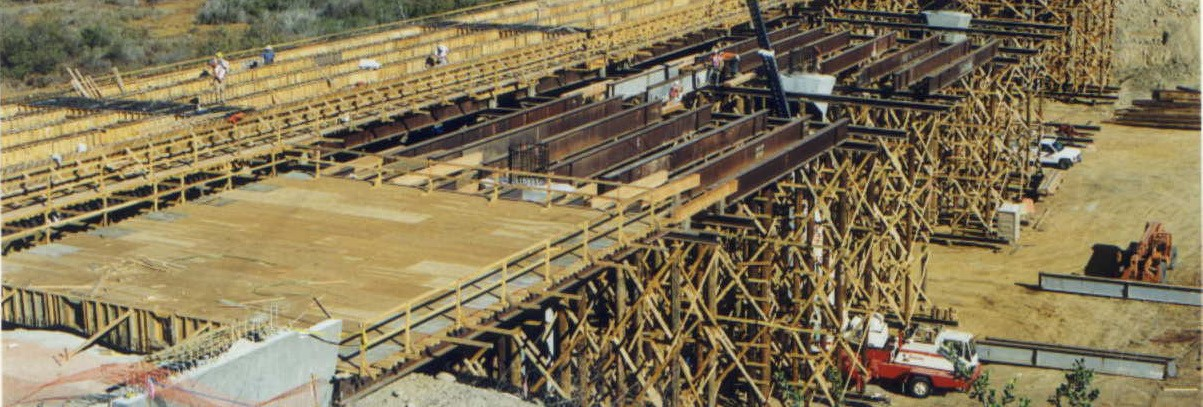
\includegraphics[width=\linewidth]{cast-in-place-box-girder.jpg}
  % \caption{Cast-in-place box girder bridge on falsework. (Courtesy Atkins North America, Inc.)}
  \caption{支架现浇箱梁}
  \label{fig:cast-in-place-box-girder}
\end{figure}

\paragraph{Segmental posttensioned concrete box girders (CIP and Precast)}

Segmental concrete box girder systems have been used when span requirements are greater than what can be
achieved with conventional stringer-type girders or spliced girders, in instances of sharp horizontal curvature, or
when special aesthetics are required. They have been economical in span ranges from about 250 feet to 500 feet.
This system is further divided into cantilever construction and span-by-span construction, and can be either precast or
cast-in-place. They can be cast to match the shape of any alignment making them particularly suited to curvature.
Figure 2.17 shows a cast-in-place segmental bridge recently built in Florida using balanced cantilever construction.

Segmental box girder bridges have been observed to improve deck performance due to the pre-compression of
the deck. Refer to Chapter 3 on materials for additional information on these bridge deck systems and durability
issues relating to details currently in use.

\begin{figure}
  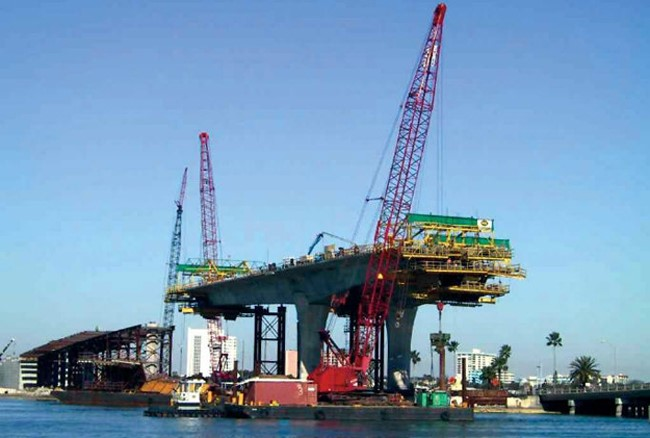
\includegraphics[height=5cm]{cast-in-place-segmental1.jpg}\hfill
  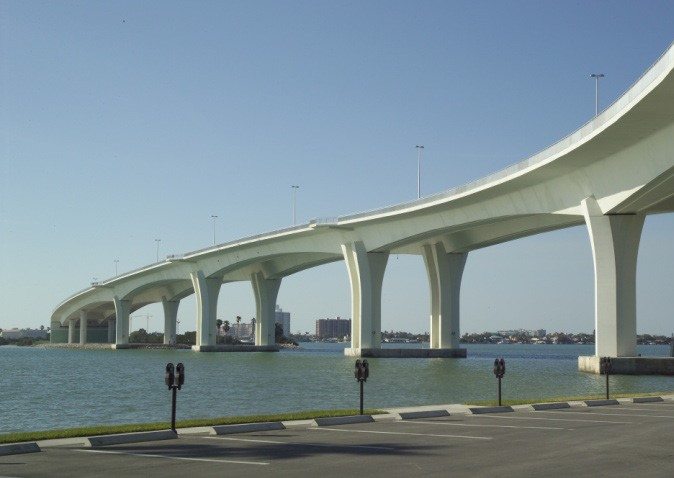
\includegraphics[height=5cm]{cast-in-place-segmental2.jpg}
  % \caption{Cast-in-place segmental concrete box system. (Courtesy HDR, right photo by John Rupe)}
  \caption{节段现浇混凝土箱梁}
  \label{fig:cast-in-place-segmental}
\end{figure}

\paragraph{Concrete Arches}

Concrete arches have been used for bridges with short spans of about 100 ft to long spans of over 1,000-ft span,
but are typically considered today only in certain long span applications because of the relative economy of I-girder
and segmental box girders in shorter spans, or when special aesthetics are required. True arches are efficient
structural systems because vertical dead load produces axial member compressive forces that are resisted by a thrust
at the arch abutments. Concrete has been useful for arches because of its inherent efficiency in compression.


Concrete arches have typically been used in deck-type systems where the arch ribs are below the deck, but they
have also been used in some through-type applications where the arch ribs extend above the deck. Deck arch
systems are either closed spandrel types or open spandrel types. Closed spandrel types typically use barrel arches
with longitudinal walls along the outside edges of the arches that are either filled or unfilled. Open spandrel types
have a series of spandrel columns that transmit deck loads to the arches.


Concrete arches in the U.S. have typically been constructed using either cast-in-place on falsework methods or
cable-stayed segmental methods. \cref{fig:hoover-dam} shows the cable-stayed, cast-in-place segmental construction method
used for the Hoover Dam Bypass concrete arch bridge.

\begin{figure}
  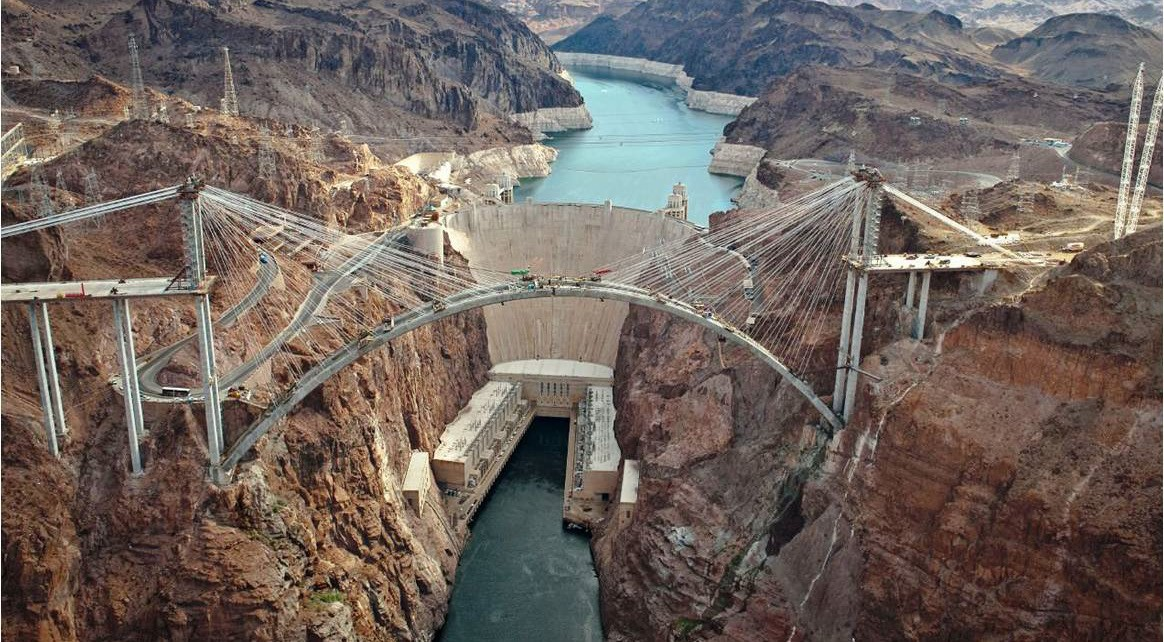
\includegraphics[width=\linewidth]{hoover-dam.jpg}
  % \caption{Hoover Dam Bypass concrete arch bridge constructed using cable-stayed segmental methods. (Courtesy HDR, photo by Keith Philpott)}
  \caption{胡佛水坝旁路采用斜拉分段法建造的混凝土拱桥}
  \label{fig:hoover-dam}
\end{figure}

\paragraph{Modular Pre-topped Concrete Girders}

These types of systems utilize precast beam elements that are fabricated with a portion of the deck in place as a
unit and are erected side by side and connected with a CIP closure joint, posttensioning, composite concrete topping,
or a combination of these methodologies. The precast elements commonly consist of conventionally-reinforced or prestressed sections that include T beams, double Ts, and deck bulb-tees. This system is expected to gain popularity
with accelerated bridge construction as pressure mounts to expedite construction and to minimize field forming and
placing of concrete. Refer to Chapter 4, Bridge Deck, for information concerning CIP closure connections.

A recent concept is the NEXT Beam (Northeast EXtreme Tee), which was developed by the Precast/Prestressed
Concrete Institute North East (PCINE) along with the Departments of Transportation for New York, Connecticut,
Massachusetts, Vermont, Maine, New Hampshire, and Rhode Island (Culmo and Seraderian 2010). It is a precast,
prestressed double-tee section with 8-ft or 12-ft deck widths, and beam depths from 24 in. to 36 in. that is applicable
for approximately 40-ft to 90-ft spans. It is available with a thick top flange that comprises the deck, or with a top
flange that creates a form for a composite CIP deck. The NEXT beam is considered as an alternative to traditional
adjacent concrete box beams, providing improved durability, lower cost, easier inspection and accelerated bridge
construction.

% \subsection{Substructure Componet}
\subsection{下部结构\glsentrytext{componet}}

The substructure component includes all structural elements required to support the superstructure and is typically defined from the underside of bridge bearings down through the foundation. The function of these elements is to transfer all vertical loads from the superstructure to the foundation supporting strata and to resist horizontal forces acting on the bridge. The transfer of load to the supporting ground can be either through spread foundations, piles, or drilled shafts, depending on the strength and stability of subsurface geotechnical conditions. This component typically includes pier and abutment subsystems, each including several elements, as shown in \cref{fig:substructure-component}.

\begin{figure}
  % \includegraphics[width=\linewidth]{substructure-component.pdf}
  \caption{Substructure component}
  \label{fig:substructure-component}
\end{figure}

% \subsubsection{Piers and Bents}
\subsubsection{桥墩与排架}

Piers are intermediate supports for multi-span bridges. They can have multiple configurations, but typically fall into two major categories, piers and bents, as illustrated in Figures 2.20 and 2.21. A pier subsystem consists of several elements, including a cap beam supporting the main load-carrying elements of the superstructure, which in turn is supported on one or more columns. The columns are supported by foundations that are typically located at or below the finish grade of the adjacent ground. The foundation can be a footing bearing directly on rock or soil, or a deep foundation using piles or drilled shafts.

T-piers are examples of single column piers with a cap element. Solid- or wall-type piers are also single column piers, but are wide enough to support the superstructure without having a separate cap element.

A bent consists of a cap beam supporting the main load-carrying elements of the superstructure, which in turn is supported directly on deep foundation elements such as piles or drilled shafts that extend up from finish grade. In some cases, the term “bent” is also used to describe a multi-column pier.

Common practice is to construct piers with reinforced concrete, although some steel piers with pier caps have been used. When deep foundations are required to support the bent caps, they normally consist of timber, prestressed concrete square, solid round or hollow cylinder piles, CIP concrete drilled shafts, or steel HP or steel pipe sections.

Modular, precast concrete pier elements have also been used for accelerated construction.

\begin{figure}
  \begin{minipage}{0.48\linewidth}\centering
    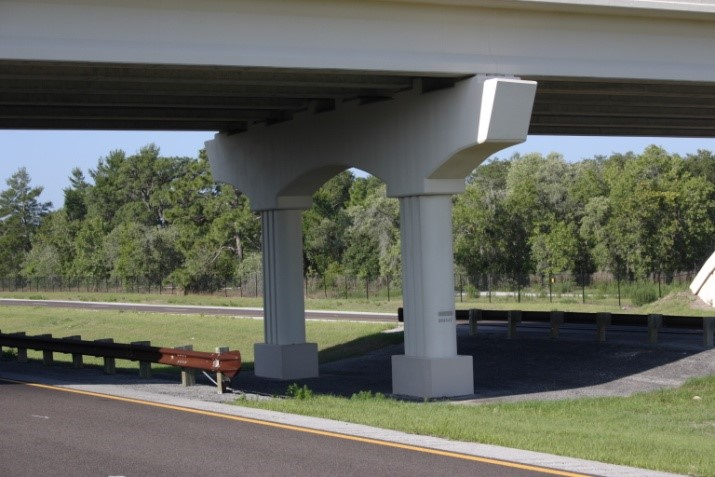
\includegraphics[height=4.5cm]{piertype1.jpg}
    \subcaption{多柱式桥墩}
  \end{minipage}\hfil
  \begin{minipage}{0.48\linewidth}\centering
    \includegraphics[height=4.5cm]{piertype2.jpg}
    \subcaption{排架桩}
  \end{minipage}
  % \caption{Pier types: multi-column supported pier and pile bent. (Courtesy Atkins North America, Inc.)}
  \caption{桥墩类型:多柱式桥墩和排架桩。}
  \label{fig:piertypes-multi}
\end{figure}

Integral pier cap construction was also developed as a way to avoid sharp skews or associated longer spans in interchange ramp bridges, and to lower overpass profiles. Integral pier caps also have the advantage of eliminating bearings, which can minimize future maintenance requirements. \cref{fig:piertypes-integral} shows a ramp bridge with conventional stacked T-pier construction and a similar ramp bridge with integral pier construction. Integral pier system is advantageous in seismic areas by integrating the super structure and substructure and creating frame action.

\begin{figure}
  \begin{minipage}{0.48\linewidth}\centering
    \includegraphics[height=4.5cm]{piertype3.jpg}
    \subcaption{常规 T 型桥墩的匝道桥}
  \end{minipage}\hfil
  \begin{minipage}{0.48\linewidth}\centering
    \includegraphics[height=4.5cm]{piertype4.jpg}
    \subcaption{整体式桥墩的匝道桥}
  \end{minipage}
  % \caption{Conventional and integral pier types. (Courtesy HDR)}
  \caption{常规和整体式桥墩类型}
  \label{fig:piertypes-integral}
\end{figure}

% \subsubsection{Abutments}
\subsubsection{桥台}
Abutments are provided in multiple configurations, but can be defined in two major categories as illustrated in \cref{fig:abutmenttypes}:
\begin{itemize}
  \item Stub or spill-through abutments, and
  \item Full abutments.
\end{itemize}

\begin{figure}
  \begin{minipage}{0.48\linewidth}\centering
    \includegraphics[height=4.5cm]{abutment1.jpg}
    % \subcaption{Stub or spill-through abutment.}
    \subcaption{墩式溢流型桥台}
  \end{minipage}\hfil
  \begin{minipage}{0.48\linewidth}\centering
    \includegraphics[height=4.5cm]{abutment2.jpg}
    % \subcaption{MSE full abutment.}
    \subcaption{全 \acrshort*{mse} 桥台.}
  \end{minipage}
  % \caption{Abutment types. (Courtesy Atkins North America, Inc.)}
  \caption{桥台类型}
  \label{fig:abutmenttypes}
\end{figure}

Stub abutments are characterized by sloped embankments under the end span of the bridge and provide support to the superstructure through a shallow bent cap resting on a pile foundation.

Traditionally, full abutments are characterized by a vertical wall that retains the embankment fill and also transfers the bridge load to the supporting foundation at the base of the wall. Full abutments can also be in the form of a \acrfull{mse} system, which employs a fascia wall connected to a system of reinforcing elements in multiple layers that work with the backfill material to create a composite soil mass. This composite soil mass can then support vertical load and/or act as an earth retention system. There are two types of MSE abutments: true or mixed (Anderson and Brabant 2010). In a true MSE abutment, the bridge superstructure is supported on spread footings bearing directly on the top of the reinforced soil mass. In a mixed MSE abutment, a shallow bent cap with a row of piles is used to support the superstructure behind the MSE fascia wall, and the reinforced soil mass is used to retain the fill behind and adjacent to the end of the bridge. A MSE full abutment is pictured in \cref{fig:abutmenttypes}.

Another recent form of abutment system is the \acrfull{grsibs}, which is described in FHWA publication FHWA-HRT-11-027 (Adams et al. 2011). This is a relatively new abutment system that has been used for accelerated bridge construction, and typically for short spans up to about 140 feet. The abutment uses alternating thin layers of compacted fill and geosynthetic reinforcement sheets that combine to form a reinforced soil mass foundation that directly supports the bridge superstructure without the need for piles. The geosynthetic reinforcement is connected into layers of precast facing blocks that are placed with the reinforcement and soil backfill. Once completed, the reinforced soil mass is ready to support the bridge.

Traditional abutments are typically concrete construction. When deep foundations are required to support the bent caps, they normally consist of timber, prestressed concrete square, solid round or hollow cylinder piles, CIP concrete drilled shafts, or steel HP or pipe pile sections.

Types of abutments used also characterize the way the entire bridge system responds to thermally-induced longitudinal movements. There are three distinct abutment types:
\begin{itemize}
  \item Integral abutment,
  \item Semi-integral abutment, and
  \item Abutment using expansion devices.
\end{itemize}

In integral abutment systems, are attached directly to abutment, and thermally-induced longitudinal movements are accommodated by flexibility of the piles. The piles are subject to both axial and flexural moments. In semiintegral abutment systems, girders and piles are not directly connected and the bearings used to support girders and piles are mainly subject to axial loads. Integral and semi-integral abutment systems are part of different continuous bridge systems. Chapter 8 provides a more in-depth discussion, as well as detailed design provisions for integral and semi-integral abutment systems.


\section{Factors Affecting Service Life}
\label{sec:factors-affect-sl}

All of the elements, components, and subsystems that make up the overall bridge system are adversely affected in various degrees by both external and internal factors that contribute to reduced service life. External factors typically refer to loads or hazards, which can be both natural and man-made. Internal factors can pertain to such items as structure type (e.g. fracture critical), materials, and design/details.

Following is a discussion of critical factors that affect bridge service life using a fault tree analysis approach. Section 2.3.1 discusses factors that affect the overall bridge system. The following sections, 2.3.2 through 2.3.4, address specific factors affecting deck, superstructure, and substructure components. Section 2.4 addresses options to avoid or mitigate these factors.

\begin{figure}
  % \includegraphics[width=\linewidth]{factor-service-life.pdf}
  \caption{Factors affecting service life.}\label{fig:factor-service-life}
\end{figure}

\subsection{Bridge System Fault Tree Analysis}

\cref{fig:factor-service-life} shows the initial fault tree diagram that identifies factors affecting service life for a complete bridge system. (A detailed discussion of the fault tree process is included in Chapter 1.) The diagram identifies causes of, or factors affecting service life and categorizes them for consideration. In following sections, these categories are successively sub-categorized at descending levels to identify multiple contributing factors. The fault tree analysis is then continued until the basic events or lowest levels of resolution are reached and discussed. The lowest level or basic events require strategies for mitigations.

\subsubsection{Obsolescence or Deficiency}

At the highest fault level, reduced service life of a bridge system can be attributed to either obsolescence or deficiency. Obsolescence refers to reduced service life of a bridge due to issues related to how it functions, which can be further categorized as:
\begin{itemize}
  \item Operational issues related to reduced traffic capacity and safety,
  \item Physical issues related to span layout and clearances, or
  \item Loading issues related to increases in design live load.
\end{itemize}

Many bridges are replaced because of functional issues well before their full-potential service life is achieved. Significant increases in corridor traffic demand, caused by such factors as urban planning, land use, and development, can ultimately result in the functional inability of a bridge to provide required level of service, necessitating bridge widening or replacement. Vertical clearance limitations sometimes prevent existing bridges from being widened. Increased corridor traffic can also require replacement of overpass bridges to accommodate widened roadways and increased span requirements below. Major interchanges are sometimes reconstructed because of the need for increased traffic capacity.

Often, safety issues relating to inadequate lane and shoulder widths, sharp curves, and inadequate sight distances have a significant effect on service life. Changes in design live load over the life of a bridge can affect service life as it relates to the structure’s ability to safely accommodate increased load.

Service life design considerations should evaluate the potential of future operational needs, and how those needs might impact the service life of the planned facility. Risks of future obsolescence should be considered and appropriate choices should be made concerning mitigation or acceptance. Those choices should be incorporated into the design as appropriate considering life-cycle cost analysis.

Deficiency refers to reduced service life of a bridge due to damage or deterioration that can be caused by a number of primary factors and sub-factors, each of which can lead to reduced service life if un-mitigated. Deficiency can occur in all three bridge components: deck, superstructure, and substructure. In Figure 2.23, the fault tree continues below the superstructure component, but it applies equally to all three components.

Within a bridge system, the interaction between components, deficiencies, or failures within a particular component can have a significant effect on other components. A primary example is deterioration of superstructure and substructure below leaking joints in the deck component (see Section 2.3.1.3.1). Another example is damage to substructure and other superstructure elements caused by failed bearings in the superstructure component (see Section 0)

Deficiency can be further attributed to any of three major causes:
\begin{itemize}
  \item Load-induced,
  \item Natural or man-made hazards, or
  \item Defects in production/operation.
\end{itemize}

\subsubsection{Reduced Service Life due to Loads}

Load-induced deficiencies can be further categorized as those caused by traffic-induced loads or systemdependent loads (see Figure 2.24). The fault tree is continued for each of these load types to identify the basic or lowest levels causing damage or deterioration.

\begin{figure}
  % \includegraphics[width=\linewidth]{load-induced-deficiencies.pdf}
  \caption{Load-induced deficiencies}\label{fig:load-induced-deficiencies}
\end{figure}

\paragraph{Traffic-Induced Loads}

Traffic-induced loads include the effects of truck and other vehicle traffic that are applied to the bridge deck and transmitted throughout the bridge system. Traffic load can ultimately cause damage to bridge elements through
fatigue, overload, or wear.

\begin{description}
  \item [Fatigue] is structural damage to an element resulting from cyclic loading that results in the initiation and  propagation of cracks, and can occur at stress levels considerably below the yield stress. Although fatigue can occur in reinforced concrete and structural steel elements, it is more predominant in steel elements. Chapter 3 on materials discusses fatigue deterioration in reinforced concrete.

  Early-welded steel structures have a history of cracking at certain types of weld details due to load-induced and distortion-induced fatigue. Newer design provisions and recommended details have been developed that provide solutions for both load-induced and distortion-induced fatigue that will achieve desired service life. Section 2.3.3.1.1 provides additional information of fatigue in steel structures, and Chapter 7 provides a comprehensive discussion on fatigue and fracture in steel bridges.
  \item [Overload] refers to element overstress or damage resulting from over-weight vehicles that exceed maximum gross vehicle weight restrictions or individual axle or tire restrictions. Overload often results from illegal, nonpermitted vehicles and is the third leading cause of bridge failure in the U.S. behind hydraulic and impact causes (Wardhana and Hadipriono, 2003). Overload produces higher stress in members than what was considered in design,
  and can significantly reduce safety factors against failure, and can cause cracking in concrete elements. Multiple applications can also affect fatigue behavior and also result in excessive deflection that can affect certain elements, particularly in cases of differential deflection.

  Because overload occurs on many bridges, the risk of overload should be considered on certain vehicular routes when planning new bridges. It may also be necessary to consider special owner-specified loads to avoid or mitigate this risk.
  \item [Wear] refers to element damage and gradual loss of material caused by friction or rubbing. Decks are susceptible to wear from vehicle tires, especially with the use of studs or chains. Deck wear and abrasion is further discussed in Chapter 4. Wear has been a factor in steel structures, particularly on pins and pin plates in connections, and in bearings, with surface wear in sliding bearings, brass sealing ring wear in pot bearings, and pin wear in steel bearings.
\end{description}

\paragraph{System-Induced Loads}
System-induced loads include the effects of the bridge system configuration on the behavior of the structure. These effects are accentuated by restraints provided through bridge boundary conditions and can result in significant locked-in stresses. The system-induced loads can be the result of movements due to time-dependent material properties, thermal movements, or system framing restraint.

\begin{description}
  \item [Time-dependent material properties] refers mainly to shrinkage and creep-related deformations in restrained
  concrete elements and can result in concrete cracking. This phenomenon is discussed further in Chapter 4 for bridge
  decks and in Chapter 3 for concrete materials in general.
  \item [Thermal Conditions] refers to effects caused by temperature change, which can result in significant stresses in
  restrained structural members, and can be as large as live load stresses in some cases. The effects can be the result of
  uniform stress across a bridge member, or the result of a temperature gradient throughout the depth of a member.
  \item [System-framing restraint] refers to effects caused by boundary condition restraints that prevent normal or
  intended structural behavior. Improper function or seizing of bearings can result in unintended movement restraint,
  which can further cause pier cracking and distress. Another example occurs at ends of skewed integral abutments,
  where lateral movement resulting from the skew can cause cracking and distress in corner details if adequate
  clearance is not provided to allow for the movement.
\end{description}

\subsubsection{Reduced Service Life due to Natural or Man-Made Hazards}

Environmental hazards from both natural and man-made sources can have a significant influence on bridge
service life. These also include effects from areas with adverse thermal climate, coastal climates, and chemical
climates, as well as from chemical properties of the materials themselves. Other hazards such as hydraulic action,
collisions, fire/blast, or seismic events can also have considerable effect. These natural and man-made hazards are
introduced in the fault tree shown in \cref{fig:natural-man-made-hazards}.

\begin{figure}
  % \includegraphics[width=\linewidth]{natural-man-made-hazards.pdf}
  \caption{Natural or man-made hazards}\label{fig:natural-man-made-hazards}
\end{figure}

\paragraph{Thermal Climate}
Deicing salts corrosion. Bridge service life is typically severely affected in cold, wet climates due to heavy use
of roadway deicing salt. Salt-contaminated moisture penetration directly affects bridge deck service life by initiating and propagating corrosion in unprotected reinforcing steel, and by accelerating concrete deterioration due to cracking
and freeze/thaw damage. All unprotected bridge elements below open or leaking deck joints are subject to saltcontaminated
roadway drainage, which causes unprotected structural steel corrosion, concrete reinforcing bar
corrosion, and associated concrete cracking and spalling.

On overpass bridges, salt spray rising from roadways below affects superstructures and undersides of decks,
causing concrete penetration and corrosion of unprotected reinforcing, and corrosion of unprotected structural steel.
The salt spray from vehicles passing underneath the bridge can also affect the service life of weathering steel by
keeping the steel continuously wet.

Decks, barriers and deck joints are also susceptible to damage from snow plows used to clear roadways for
traffic.

Freeze/Thaw. Water absorbed into concrete surfaces and contained in cracks can freeze in cold weather
conditions. The frozen water tends to expand causing stresses within the concrete. Cyclic freezing and thawing of the
water absorbed in the deck surface fatigues the concrete, resulting in cracking, scaling, and spalling. Refer to
Chapter 3 on materials for additional information on freeze/thaw in concrete.

\paragraph{Coastal Climate}
Salt water/spray corrosion. Coastal saltwater environments also have severe effects on bridge service life due
to wetting and chloride penetration causing corrosion of unprotected reinforcing, and corrosion of unprotected
structural steel.

Structures in these areas are subjected to a chloride-laden saltwater environment and a combination of wind and
wave action that causes these chlorides to become airborne as salt spray. The susceptibility of various bridge
components to these environmental influences depends on their degree of direct contact or their height above the
water elevation. Pier columns with direct contact in areas of continual wetting are most susceptible to damage.

Wave action hitting substructure units and seawalls or abutments under the bridge also tend to cause the salt
spray to explode upward, wetting the bottoms of lower level superstructures and decks. The salt spray can also
deposit itself on the bridge deck surface, particularly on windy days. The salt spray wets the surfaces leaving a
chloride residual that can absorb into the concrete, resulting in reinforcement corrosion that in turn causes cracking, spalling, and/or delamination. The wet salt spray can also be deposited on the sides of structural steel members
affecting service life of coatings, and directly causing and accelerating steel corrosion.

Humidity. High humidity in coastal regions also results in cyclic wetting and drying of bridge surfaces. Concrete
materials sensitive to repeated wetting, such as those in which reactive aggregates are utilized, can have an adverse
effect on concrete elements. Continuous wetting and drying also affects coatings on structural steel members and
causes steel corrosion.

\paragraph{Chemical Climate}

Corrosion-inducing chemicals. Chemical climate influences on bridge service life performance can be
attributed primarily to airborne corrosion-inducing chemicals as a result of nearby industrial facilities such as
chemical plants or oil and coal-burning facilities. Chapter 3 provides further discussion on chemical influences on
concrete, and Chapter 6 discusses the influence of corrosion-inducing chemicals with respect to steel coatings and
steel corrosion.

Sulfate attack. Exposure to sulfates can cause expansion of concrete material that can cause spalling and
cracking, and the loss of bond strength between the cement paste and aggregate. Refer to Chapter 3 for additional
information on sulfate attack in concrete.


\paragraph{Reactive Materials}

Reactive ingredients with the concrete mix can affect concrete service life performance by altering the
volumetric stability of the concrete mix design. These influences primarily occur naturally.

Alkali-silica reactivity (ASR) results in swelling of aggregate particles within concrete that can lead to spalling,
cracking and general concrete deterioration. Chapter 3 provides additional information on ASR in concrete.

Alkali-carbonate reactivity (ACR) results in aggregate expansion within concrete that can lead to spalling,
cracking and general concrete deterioration. Refer to Chapter 3 for additional information on ACR in concrete.

\paragraph{Hydraulic Action}

Hydraulic action is the leading cause of bridge failure in the United States (Wardhana and Hadipriono 2003).
The two principal base elements are flood/storm surge and scour.

Flood/storm surge. Floods and storm surges can significantly affect bridge service life, and can dislodge spans
from their bearings and wash them away. Storm surges during major hurricanes are most often the cause of bridge
damage, as occurred in 2005 during Hurricane Katrina, which devastated the Gulf coastline from Louisiana to the
Florida Panhandle, and damaged nearly 45 bridges (Padgett et al. 2008). Most of the damaged bridges were adjacent
to water and damage resulted from storm surge-induced loading. Much of the damage was to superstructures, where
typical damage included unseating or shifting of decks and failure of bridge parapets. Several bridges suffered
damage due to impact from loose barges and debris. The most common severe failure was unseating, which often
occurred in low elevation spans. The deck displacements were attributed primarily to a combination of buoyant
forces and pounding waves. Superstructure damage largely depended on the connection type between the decks and
bents and the bearings often provided no apparent positive connection between the superstructure and substructure.

\cref{fig:bridges-washed-out} shows the I-10 bridges across Escambia Bay in Florida that were dislodged during a storm in 2006.
Damage due to superstructure unseating was similar to that experienced in the Katrina bridge damages.

Bridges with low vertical clearance over a waterway can also be vulnerable to damage resulting from debris flow
in a flood.

\begin{figure}
  \includegraphics[width=0.5\linewidth]{bridges-washed-out.jpg}
  % \caption{Florida I-10 Escambia Bay bridges washed out during storm. (Courtesy Florida DOT)}
  \caption{佛罗里达州 I-10 埃斯坎比亚湾桥梁在暴风雨中被冲毁}
  \label{fig:bridges-washed-out}
\end{figure}

Scour. Scour is defined as the erosion or removal of streambed or bank material from bridge foundations due to
flowing water. Although scour can occur at any time, bridge scour most often results during floods where swiftly
flowing water has more energy than calm water to lift and carry sediment down river. A hole is created adjacent to
the pier or abutment when material is washed away from the river bottom exposing or undermining footings, which can compromise the integrity of the structure and lead to failure. Figure 2.27 shows an example of abutment scour.
See Section 2.3.4 for factors affecting service life of bridge substructures.

\begin{figure}
  \includegraphics[width=0.5\linewidth]{abutment-scour.jpg}
  % \caption{Abutment scour. (Courtesy U.S. Geological Survey, photo by Bill Colson)}
  \caption{桥台冲刷}
  \label{fig:abutment-scour}
\end{figure}

\paragraph{Extreme Events}
\subparagraph{Vehicle/Vessel Collision}
Vehicle/vessel collision is second to hydraulic effects as the leading cause of bridge failures (Wardhana and
Hadipriono 2003). Bridges crossing other roadways with minimum or low clearance are subject to various types of
vehicle collision, particularly involving over-height vehicles. Figure 2.28 shows the effects of a collision in which a
truck transporting a hydraulic crane with the boom inadvertently raised struck a concrete bridge and cut halfway
through the entire width of the superstructure. Piers with minimum offset from edge of roadway or shoulder are also
subject to vehicle collision if not adequately protected by barriers.

The risk of vehicle impact should be considered in the design of new bridges, particularly bridges crossing heavy
truck routes where a greater probability exists for over-height vehicles, and where there has been a history of impacts
from over-height vehicles. Possible mitigation strategies include:
\begin{itemize}
  \item Using higher clearances,
  \item Using sacrificial beams to protect load carrying members, and
  \item Using laser detection systems that set off warning signals if an over-height vehicle is detected.
\end{itemize}

\begin{figure}
  \includegraphics[height=6.5cm]{bridge-impacted-by-truck1.jpg}\hfill
  \includegraphics[height=6.5cm]{bridge-impacted-by-truck2.jpg}
  % \caption{Bridge impacted by truck transporting hydraulic crane. (Courtesy Kansas DOT)}
  \caption{运输液压起重机的卡车撞击桥梁}
  \label{fig:bridge-impacted-by-truck}
\end{figure}

Bridges crossing water bodies or waterways are subject to ships colliding with either piers or superstructure.
They are rarely occurring extreme events, but have potentially high consequences. \cref{fig:ship-collision} shows the aftermath
of a ship collision with the original Sunshine Skyway Bridge in Florida. The ship collided with one of the end piers
in the main channel 3-span unit, took out the pier and subsequently the superstructure unit.

Considerations for new bridges should evaluate span openings required for safe navigation, including horizontal
and vertical clearances, and consider appropriate mitigation measures to reduce the risk of collision. Adequate
fender systems or other pier protection devices also need to be considered where there is risk of ship collision.

The current AASHTO LRFD Bridge Design Specifications (LRFD Specifications) provide requirements for new bridge design for both vehicle and ship impact (AASHTO 2012).

\begin{figure}
  \includegraphics[width=0.8\linewidth]{ship-collision.jpg}
  \caption{阳光高架桥因船舶碰撞而倒塌}
  \label{fig:ship-collision}
\end{figure}

\subparagraph{Fire}
Fires, as extreme-event hazards for bridges, have a low probability of occurrence, but can cause significant
damage to affected bridge components including the deck, superstructure, and substructure, and can cause collapse of
entire spans. Although considered a low risk hazard, a recent study by the New York Department of Transportation
(DOT) in 2008 showed that nearly three times more bridges have collapsed because of fire than earthquakes (Kodur
et al. 2010).

Fires affecting bridges most typically occur due to vehicle accidents either on a bridge or on a roadway or
railway crossing below a bridge, but can also occur due to fires in adjacent buildings or facilities. Fires can vary in
intensity, the most intense due to accidents with tanker trucks or railroad tanker cars carrying large quantities of
highly flammable fuels or chemicals. The temperature of a recent fire below a bridge that was caused by a railroad
tanker car collision loaded with 30,000 gallons of Methyl Alcohol was estimated to be approximately 3000°F
(Stoddard 2002). Recent bridge fires involving tanker trucks carrying diesel fuel and gasoline were reported to have
reached temperatures over 2,000°F (Kodur et al. 2010).

The extreme high temperatures generated in these types of bridge fires for prolonged periods of time can
significantly affect both steel and concrete structures. Figure 2.30 shows examples of dramatic bridge fires caused by
gasoline tanker truck accidents.

Steel bridge elements are especially vulnerable to high temperatures because of steel’s high thermal conductivity
in which the temperature of unprotected steelwork will vary little from that of the fire. These cases can result in loss
of strength, significant sagging, and possible collapse. Steel starts to loose strength at about 600° F, and its strength
is reduced to about half its yield strength at about 1,100°F (Brandt et al. 2011). At about 1,700° F, the yield strength
is only about 10\% or less. When fires at steel bridge elements reach these extreme temperatures, significant
deformation and sagging usually occurs (if not total collapse) and the affected bridge elements will typically have to
be replaced. Figure 2.31 shows extreme sagging in a steel bridge span and heavy concrete pier deterioration after a
gasoline tanker truck fire.

\begin{figure}
  \includegraphics[width=0.6\linewidth]{tanker-truck-accident.jpg}
  % \caption{Intense bridge fire due to tanker truck accident. (Courtesy U.S. Fish and Wildlife Service)}
  \caption{油罐车事故导致桥梁大火}
  \label{fig:tanker-truck-accident}
\end{figure}
\begin{figure}
  \includegraphics[width=0.8\linewidth]{tanker-truck-collision.jpg}
  % \caption{Steel bridge heavily damaged by fire after gasoline tanker truck collision. (Courtesy Alabama DOT)}
  \caption{钢桥在汽油罐车碰撞后被火灾严重损坏}
  \label{fig:tanker-truck-collision}
\end{figure}

In cases where damage to steel bridges sustained during a fire is not obvious (i.e., no clear signs of distress such
as sagging or buckling) the question is often raised as to whether permanent material property effects in heat affected
areas has occurred. It has been reported that steel will begin to encounter phase changes at temperatures greater than
1,300°F, whereby undesirable material properties such as reduced ductility and toughness can result during
uncontrolled cooling. The Pennsylvania DOT sponsored a study to examine the effects of fire damage on the
structural properties of steel bridge elements (Brandt et al. 2011). The study performed fire tests on painted steel
plate specimens at various temperatures up to 1,200°F and exposure times to evaluate changes in surface conditions
and discoloration and to then test for changes in material properties after cooling. The results showed that up to steel
surface temperatures of 1,200°F, the fire-exposed material after cooling still satisfied AASHTO material
specifications. They further concluded that if excessive distortions or deformations occurred, the steel would likely
have been subjected to steel temperatures well in excess of 1,200°F, and the corresponding sections would require
replacement.

Concrete bridge elements are typically able to withstand high temperatures with less distress than unprotected
steel elements. Concrete has inherent fire resistant properties due to its relatively low thermal conductivity, which
insulates interior portions of the member including reinforcement and/or prestressing steel from high surface
temperatures. Concrete does experience a reduction in strength and modulus of elasticity with high temperature.
Strength reduction is largely a function of type and size of aggregate. Concrete with siliceous aggregate (materials
consisting of silica and including granite and sandstone) begins to lose strength at about 800°F, and is reduced to about 55\% at 1200°F. Concrete containing light-weight aggregates (manufactured by heating shale, slate, or clay)
and carbonate aggregates (include limestone and dolomite) retain most of their compressive strength up to about
1200°F (Bilow and Kamara 2008). The following compares concrete temperature with typically encountered signs
of distress and concrete color (Shutt 2006).

\begin{itemize}
  \item Up to 200°F—little or no concrete damage;
  \item 500°F—surface crazing, localized cracks, iron bearing aggregates begin to acquire pink/red color;
  \item  700°F—cracks appear around aggregate, numerous micro cracks present in cement paste;
  \item  900°F—purple/gray color appears if enough iron and lime are present;
  \item  1,000°F—serious cracking of paste and aggregates occurs due to expansion. Purple/gray color may become
  more pronounced;
  \item  1,500°F—cement paste is completely dehydrated with severe shrinkage cracking and honeycombing.
  Concrete may begin to become friable and porous;
  \item  2,200°F—some components of concrete begin to fail; and
  \item  2,500°F—Concrete is completely failed.
\end{itemize}

In all cases, fire damaged structures should be evaluated as quickly as possible once the fire is extinguished to
determine the extent and severity of damage. Limits of concrete damage can often be tested with an impact-rebound
hammer. Concrete core samples can be taken for petrographic examination, which will determine the extent of
damage within the overall concrete matrix. Steel coupons can be taken to evaluate changes in material properties.

\subparagraph{Blast}

The possibility of terrorism against our nation’s bridges is an ever-increasing threat in today’s society. The risk
of blast attack is typically considered very low for most bridges, but major bridges or bridges along major corridors
that have high economic and/or socio-political impact can have greater risk. By their nature, bridges are very
accessible to vehicles carrying explosive devices traveling either on the bridge or below on crossed roadways. They are also susceptible to ships or boats carrying explosive devices below. Because bridges also vary in type and size,
the assessment of blast vulnerability can be very complicated. Until recently, there has been little work done or
information available concerning the effects of blasts on highway bridges or methods of analysis.

Extensive research is being undertaken by the FHWA (Duwadi and Munley 2011) to further understand the
behavior and effects of blast loadings on bridge elements. Part of these studies is also to develop methods for
evaluating risk and risk-mitigation strategies. The most significant research in the area of blast-resistant design
guidelines for highway bridges is being conducted under the NCHRP, project number NCHRP 12-72, which has been
recently documented in NCHRP Report 645 (Williamson et al. 2010). The response evaluation of reinforced
concrete bridge columns was a key part of this investigation. Other recent research reported by Agrawal and Yi,
2008, dealing with blast load effects on highway bridges developed computer models and showed through simulation
analysis that seismic capacities and blast-load effects are strongly correlated. Kiger et al. 2010, reported on bridge
vulnerability assessment and mitigation against explosions, and focused on response of posttensioned box girder
bridges under blast loads.

Blast loads are considered one of the extreme hazards affecting bridges, and even a small amount of explosive
can produce severe localized damage to a bridge element. In some cases, this localized damage can potentially
progress to global collapse of the structure (Kiger et al. 2010). There are a number of factors that affect the potential
damage to a bridge due to blast, including:

\begin{itemize}
  \item Size and type of explosive charge. Small explosive devices can have varied effects depending on placement
  and size of bridge element, but large truck bombs can be disastrous. The Oklahoma City Federal Building
  bombing in 1995 is an example of the devastating effect a large truck bomb.
  \item Proximity to blast—standoff distance. The distance from the blast to a bridge element is a critical parameter
  in determining the blast effect. For a given size blast, the effect will reduce significantly with relatively
  small increases in distance from the blast.

  Depending on the size and standoff distance, three blast categories exist: contact, close in, and plane wave
(Williamson et al. 2010). Contact blasts are very close and create high intensity, non-uniform loads where
breaching, or complete loss of material at a section in a bridge element, can occur. In this case, there can be extensive local destruction. A close in blast is farther away but still results in a localized spherical shock
wave striking the structure to produce a non-uniform load and impulse-dominated response. A plane wave
blast is far enough away to produce essentially planar shock waves and a uniform load on the structure. In
this case, the structure will be loaded in a manner that leads to global deformation, and will be resisted by the
entire structure or a number of combined elements.

\item Location of blast. Blasts can occur above or below deck. Above deck blasts can affect the deck itself, and
any structural elements above deck such as in a through truss, arch, or cable supported bridge. Blasts below
deck would typically have more effect on pier columns, but can affect superstructure if sufficiently large.
Below deck blasts can also have greater intensity because of the enclosed effect created by the overhead
structure, whereas above deck blasts have more freedom to dissipate without shock wave reflection.

\item Type and size of bridge element. Members with greater mass, hardness, and flexibility have greater blast resistance.
\item Structural redundancy. Having multiple load paths is a key factor in resisting overall structural collapse with any type of individual member failure. Multi-column piers or multi-girder superstructures are typically able to re-distribute internal forces and provide greater resistance to overall structure collapse.
\end{itemize}

A risk management approach can be taken for bridges with greater potential of fire or blast hazard. These
bridges can be identified by reviewing major corridors that would experience the greatest economical and sociopolitical
impact if damaged by these extreme event hazards. Potential mitigation including local protective measures,
alternative routes, or accelerated reconstruction strategies can be evaluated for these higher-risk bridges.

% \subparagraph{Seismic}
\subparagraph{地震}
\label{subpar:seismic}

Earthquakes, including those of moderate intensity, are extreme hazard events that can cause significant damage
to bridges, and particularly to existing bridges that were designed under older codes and have not been retrofitted.

The 1971 San Fernando earthquake in California, which resulted in numerous bridge collapses, has often been
cited as a watershed event in bridge engineering since it demonstrated the inadequacy of seismic bridge design practices of the time (Buckle et al. 2006). The FHWA became a major sponsor of bridge seismic research shortly
afterward, including research on retrofitting existing bridges.

Other subsequent major California seismic events such as the 1989 Loma Prieta and 1994 Northridge
earthquakes, and the 1995 Kobe, Japan earthquake caused significant bridge damage and collapse, which also led to
further research and understanding of bridge seismic behavior (Azizinamini and Ghosh 1997).

The observed damage and knowledge gained from these previous events, along with extensive research
undertaken since 1971, have led to significantly improved seismic bridge design specifications (AASHTO Guide
Specifications for LRFD Seismic Bridge Design, 2nd Edition, 2011 and AASHTO LRFD Bridge Design Specifications,
6th Edition, 2012), advanced concepts for seismic retrofit (Seismic Retrofitting Manual for Highway Structures: Part
1—Bridges, Buckle et al. 2006), and guidance for seismic design of foundations (LRFD Seismic Analysis and Design
of Transportation Geotechnical Features and Structural Foundations, Kavazanjian et al. 2011).

The current approach adopted in the LRFD Specifications (2012) is to design new conventional (or ordinary)
bridges for a design earthquake, or level of ground motion, that represents the largest motion that can be reasonably
expected during the life of the bridge. It implies that ground motions larger than the design earthquake could occur
during the life of the bridge, but their likelihood of happening is small. This likelihood is usually expressed as the
probability of exceedance, and it may also be described by a return period in years. The specifications call for a
design earthquake that has a 7\% probability of exceedance in 75 years (approximately 1000 year return period).
Bridges designed and detailed under these provisions may suffer damage but should have low probability of collapse.
Key principles used for the development of these specifications are that small to moderate earthquakes should be
resisted within the elastic range of the structural components without significant damage, and that large earthquakes
should not cause collapse of all or part of the bridge, although they may cause significant damage requiring
replacement.

One of the key considerations in seismic design is repairability of the damage to bridges during moderate seismic
events. Oftentimes the so-called “minor damage” may require complete replacement of the bridge. In the case of the
1995 Hyogoken-Nanbu earthquake in Kobe, Japan (Bruneau et al. 1996; Chung 1996; Shinozuka et al. 1995;
Azizinamini and Ghosh 1997) steel bridges suffered damages to superstructure elements including inadequate crossframe
detailing leading to lateral bending of the girder webs near girder ends. This resulted in major retrofit activities and the closing of major highways, such as the Hanshine Expressway, which was closed for more than a year. The
Kobe experience demonstrated that even “minor damage” to steel bridges during seismic events can result in damage
that could be very difficult to repair. Among the lessons learned is that critical elements of the bridge that are difficult
to inspect and repair must be protected from any level of damage and remain elastic during the entire seismic
excitation.

Service life design philosophy needs to be considered when following seismic design principles, by examining
the effects of repair on traffic interruption after small to moderate earthquakes. In particular, the areas with potential
to form plastic hinges, as described below, must be detailed so that the repair can proceed with little or no
interruption to traffic. The major areas of concern are substructure elements where most plastic hinges are
anticipated. The superstructure elements of the bridge are mainly kept elastic during entire seismic event.

Seismic load behavior is largely un-known; therefore, the design philosophy for buildings and bridges is to work
on behavior of the structure under known conditions. Specifically, the design objective is to predefine the damage
locations and design them accordingly by providing adequate levels of ductility. In the case of bridges, the preferred
damage locations are at the ends of pier columns (formation of plastic hinges). In the direction of traffic, it is
preferred to put columns in double curvature as shown in Figure 2.32. This allows larger portions of the pier column
(two plastic hinges vs. one for single curvature) to participate in energy dissipation.

\begin{figure}
  % \includegraphics[width=\linewidth]{graphic-file}
  \caption{Deflected shape of a 3-span bridge under longitudinal (along traffic) direction.}\label{fig:deflected-shape-longtitudianl}
\end{figure}

In the transverse direction, pier columns are usually designed to act in single curvature, as shown in Figure 2.33.

\begin{figure}
  % \includegraphics[width=\linewidth]{graphic-file}
  \caption{Deflected shape of pier column in longitudinal and transverse directions.}\label{fig:deflected-shape-longtitudianl-transverse}
\end{figure}

Under longitudinal excitation, plastic hinges are located near the top and bottom of the columns, while under
transverse excitation; the plastic hinge is located near the bottom of the pier column.

The main design feature in seismic design of bridges is to keep the superstructure elements completely elastic
during an entire seismic event. Repairing any elements of the superstructure, even “minor” damage, could be very
time consuming and result in a major interruption to traffic. The elements that should remain elastic are referred to as
protected elements in capacity design approach. The inelasticity is then forced to take place at predefined locations
within the substructure. The predefined damage locations are the weak links or fuses that control the level of forces
to be transmitted to superstructure elements. This design approach is referred to as the capacity design approach and
is routinely used for designing bridges in seismic regions.

In the capacity design approach, protected elements are designed for the largest possible force effects they might
experience, considering the over-strength that may exist because of higher actual material strength than that specified
in design.

Areas with Seismic Risk

While earthquakes are sometimes considered primarily a California or West Coast problem in the continental
United States, data produced by the United States Geological Survey (USGS) National Seismic Hazard Mapping
indicates that at least 40\% of the United States is subject to damaging, ground shaking levels (Kavazanjian et al.
2011). Since 1996, the USGS has developed and updated maps that have depicted areas in the United States with various levels of seismic risk. These maps display earthquake ground motions for various risk levels including 2\%,
5\%, and 10\% probability of being exceeded in 50 years. Figure 2.34 shows the USGS seismic hazard map depicting
peak ground acceleration (PGA) levels with a 2\% probability of being exceeded in 50 years, or a return period of
approximately 2500 years. Along with areas along the west coast, these maps further show areas of high seismic risk
in the central and eastern United States.

\begin{figure}
  \includegraphics[width=\linewidth]{seismic-hazard-map.jpg}
  % \caption{Seismic hazard map, PGA, 2\% in 50 years. (Courtesy U.S. Geological Survey)}
  \caption{地震风险区划图(\acrfull*{pga} 超越概率 50 年 2\%) }
  \label{fig:seismic-hazard-map}
\end{figure}

Performance During Earthquakes

Moehle and Eberhard, 2000, discuss various causes and types of damage that bridges experience during
earthquakes. Key factors that affect the type and severity of bridge damage include:

\begin{itemize}
  \item Close proximity to fault rupture. This results in ground motions having high horizontal and vertical ground accelerations as well as large velocity pulses.
  \item Soil conditions. Soft soil sites can significantly amplify ground motion. Soil liquefaction and lateral spreading results in permanent substructure deformations and loss of superstructure support.
  \item Structural Configuration. Bridges are most vulnerable that have excessive deformation demands in rigid,
  nonductile elements; complex or non-uniform structural configuration; curved or skewed configuration; or non redundancy..
\end{itemize}

Major types of damage include:

\begin{itemize}
  \item Unseating at joints. Superstructure expansion joints introduce a structural irregularity that can have
  catastrophic consequences. These joints can occur within a span or at substructure supports. Irregular ground
  shaking can induce superstructure movements that can cause a span to unseat. Unrestrained superstructures
  can be toppled from their supporting substructures due to shaking or differential support movement
  associated with ground motion. Bridges with short seats are especially vulnerable. Use of restrainers has
  been effective in minimizing this risk. \cref{fig:Loma-Prieta-earthquake-damage} shows a span unseating failure on the Oakland Bay Bridge
  in San Francisco during the Loma Prieta Earthquake in 1989.
  \item Superstructure damage. Superstructures typically have sufficient strength to remain elastic during
  earthquakes, and are unlikely to be the primary cause of collapse of a span. However, certain types of
  superstructure damage have been observed, including bearing damage, pounding of adjacent units at
  expansion joints, and transverse bracing or diaphragm damage.
  \item Substructure damage. Substructures typically sustain the most damage, and can be categorized by column
  failure and abutment damage.
  \begin{itemize}
    \item Column failure. The lateral load capacity of a pier is limited by the shear or flexural strength of its
    columns. For non-ductile reinforced concrete columns, shear failure is often the primary mode of failure
    when subject to large inelastic demands during strong earthquakes. Column failure is often the primary
    cause of bridge collapse during earthquakes (Moehle and Eberhard 2000).

    Most damage to columns can be attributed to inadequate detailing, which limits the ability of the column
to deform inelastically. In concrete columns, detailing inadequacies can produce flexural, shear, splice,
or anchorage failures. In steel columns, local buckling has been observed to lead progressively to
collapse (Moehle and Eberhard 2000). \cref{fig:Loma-Prieta-earthquake-damage} shows a non-ductile column shear failure on the Cyprus Street Viaduct in San Francisco that
occurred during the Loma Prieta Earthquake in 1989.
    \item Abutment damage. Damage to shear keys and wing walls is often prevalent.
  \end{itemize}
\end{itemize}

\begin{figure}
  \begin{minipage}{0.55\linewidth}\centering
    \includegraphics[height=8cm]{lomaprieta1.jpg}
    % \subcaption{Oakland Bay Bridge upper roadway span unseating and    collapse.}
    \subcaption{奥克兰海湾大桥上部车行道跨度脱落和倒塌}
  \end{minipage}%
  \begin{minipage}{0.45\linewidth}\centering
    \includegraphics[height=8cm]{lomaprieta2.jpg}
    % \subcaption{Cyprus Street viaduct support column collapse}
    \subcaption{Cyprus 高架桥支撑柱倒塌}
  \end{minipage}
  % \caption{1989 Loma Prieta earthquake damage near San Francisco, California. (Courtesy U.S. Geological Survey)}
  \caption{1989 年加利福尼亚州旧金山附近的 Loma Prieta 地震造成的破坏}
  \label{fig:Loma-Prieta-earthquake-damage}
\end{figure}

\subsubsection{Reduced Service Life due to Production/Operation Defects}

Decisions made for the production of bridges and activities during its operation can have a significant influence
on overall bridge service life. These production and operation influences are introduced in the fault tree provided in
\cref{fig:production-operation-defects}, and include decisions made during the design and detailing of the bridge, quality of fabrication and /or
manufacturing, quality of construction, the level of inspection performed during operations, and the level and quality
of maintenance. Each of these categories can be further developed to identify the lowest or basic levels causing
deficiency, but these lower levels can vary significantly for each bridge system, component, or element type. The
discussion here will address general issues that are common to all.


\begin{figure}
  % \includegraphics[width=\linewidth]{graphic-file}
  \caption{Production or operation defects}
  \label{fig:production-operation-defects}
\end{figure}

\paragraph{Design/Detailing}
Decisions made during the system selection, design, and detailing phase of a bridge project can significantly
impact the service life of the bridge. It is incumbent upon designers to understand the implications of these decisions
in order to help in making rational choices that will improve service life.

Examples of design/detail issues causing reduced service life include:
\begin{itemize}
  \item Using bridge systems with deck joints that can ultimately leak and cause service life issues below. See
  Chapter 8 on jointless bridges.
  \item Providing inadequate drainage systems that allow moisture to remain on bridge decks, leading to
  deterioration, or improper layout, capacity, or slopes on drainage elements that ultimately lead to clogging
  and malfunction.
  \item Dealing with moisture trap details on steel bridges that hold water and debris resulting in coating damage and
  steel corrosion. See Chapter 6 on corrosion protection of steel bridges
  \item Using fatigue-prone details.
  \item Considering design errors. Effective quality assurance (QA) and quality control (QC) in design process is
  necessary to avoid errors.
\end{itemize}

\paragraph{Fabrication/Manufacturing}
Defects in fabrication or manufacturing can lead to reduced service life in steel or concrete bridge elements.
Undetected fabrication defects can lead to fatigue damage in steel structures.

\paragraph{Construction}
Defects or damage in construction can reduce service life in steel or concrete bridge elements. Poor concrete
placement and curing practices can have significant effects. See Chapter 3 on material and Chapter 4 on decks for
further discussion on concrete placement.

Transportation and erection of both steel and concrete girders can become an issue if not handled properly. As
high-performance materials are increasingly used for bridge construction (HPS and/or HPC), girders tend to become
longer and their webs slimmer. Transportation of these girders can then cause higher stresses or out-of-plane
bending, which can result in cracking. Girder stability during erection, particularly in curved steel girders, needs to
be carefully addressed.


\paragraph{Inspection}
Proper inspection during bridge operation is essential to identify defects and issues early, before more serious
conditions develop.

\paragraph{Maintenance}
Lack of or inadequate maintenance can allow deterioration to initiate throughout the bridge system and develop
into serious conditions whereby the only alternative is costly component or element replacement. Applying the
appropriate bridge preservation treatments and activities at the appropriate time can extend bridge service life at a
lower lifetime cost (FHWA 2011).

FHWA publication FHWA-HIF-11042 (FHWA 2011) provides general guidance on the importance and benefits
of preventive maintenance as part of an overall bridge preservation program. Examples of various cost-effective
preventive maintenance activities that can be applied to decks, superstructure, and substructure components are
further discussed in Section 2.4.1.3.

\subsection{Factors Affecting Service Life of Deck Componet}\label{subsec:factors-affect-deck}
The deck component includes several elements as described in Section 2.2.2.

\begin{description}
  \item [Bridge deck] service life and the factors affecting service life are described in detail in Chapter 4. Concrete
  bridge decks are particularly affected by thermal and coastal environments in which chloride penetration can cause
  reinforcing steel corrosion leading to concrete cracking and spalling. This cracking can cause the concrete
  surrounding the steel reinforcement to reach the corrosion threshold limit in environments where the top of the bridge
  deck is exposed to chlorides, such as deicing salts. Other concrete deck issues include wear and freeze/thaw damage.
  \item [Bridge expansion devices] commonly referred to as bridge joints, are discussed in Chapter 9.
  \item [Drainage systems] are most affected by lack of maintenance that causes clogging and malfunction.
  \item [Bridge railings] are affected by wet chloride environments that cause corrosion of reinforcing steel and concrete
  cracking and spalling in concrete railings. This condition is exacerbated at cold joints between the concrete barrier
  and top of slab, where salt moisture can easily penetrate and cause reinforcing corrosion. The same environments
  cause corrosion of steel railings.
\end{description}

\subsection{Factors Affecting Service Life of Supersturcture Componet}
\subsubsection{Steel Superstructures}
\paragraph{Load-Induced Deficiency—Fatigue and Fracture}
Early-welded steel structures have a history of cracking at certain types of weld details due to load-induced and
distortion-induced fatigue. Cracking at I-beam cover plate terminations or at other longitudinal weld terminations in
tension zones has been particularly evident. Cracking in girder webs due to out-of-plane bending within stiffener web
gap regions next to cross frame attachments also became a common problem. Subsequently, extensive research and
laboratory testing has provided an understanding of fatigue behavior, and different weld detail types were found to
have varying levels of fatigue susceptibility. Newer design provisions and recommended details were developed that
provide solutions for both load-induced and distortion-induced fatigue that will achieve desired service life.


Steel bridges can fail by fracture, which is the rapid, unstable propagation of a larger flaw, most likely the result
of fatigue. Fatigue crack initiation is independent of steel type and strength, but possible brittle fracture is influenced by steel toughness among other variables. Early steels were more susceptible to brittle fracture, but in recent years,
new high-performance steels—HPS 50W, 70W, and 100W—have been developed with very high toughness
characteristics. Although somewhat more costly than conventional-grade steels, high-performance steels are now
encouraged where applicable, particularly in non-redundant or fracture-critical applications. Use of high-performance
steel allows time for any fatigue cracks that may have developed to be found during regular bridge safety inspections
before fracture can occur.

Fatigue should not be an issue in new steel bridges designed in accordance with the latest LRFD Specifications.
Extensive research has been done in recent years to identify causes and solutions for fatigue- and fracture-related
problems. When using proper details and fabrication methods, both load-induced and distortion-induced fatigue
problems should not be an issue in achieving desired service life.

\paragraph{Deficiency Due to Natural or Man-Made Hazards—Corrosion}
Corrosion is a fundamental limitation of steel as a construction material, and is the result of exposure to oxygen
and moisture. The process is greatly accelerated in the presence of chloride ions from roadway deicing salt or salt
spray in a marine environment. Deck drainage with deicing salt leaking through open deck joints is a leading cause of
steel element corrosion in bridges.

Corrosion control should be designed into the overall steel bridge system. Use of systems that eliminate or
minimize deck joints will have a significant effect in reducing corrosion. Details that serve to protect and keep the
steel dry should be included in the design. Among these are bridge system solutions that eliminate deck joints,
preventing salt-contaminated drainage from reaching steel elements below.

Salt marine environments or locations subject to deicing salt spray from below also create harsh environmental
conditions subject to corrosion; thorough cleaning and zinc-rich primer coating systems can provide long-term
protection. However, requirements for related long-term coating maintenance cannot be overlooked, and must also be
designed into an overall corrosion protection plan.

To achieve long-term bridge durability, a corrosion resistance plan must be a design requirement for every new
or rehabilitated steel structure. This plan should include the use of “best painting practices” and a maintenance plan
that addresses painting priorities and timetables.

Best painting practices now include paint systems that contain metallic zinc as the corrosion-resistant pigment.
Zinc coatings provide “galvanic protection” to the steel, in which zinc (the more noble metal) will oxidize (corrode)
in preference to the steel. To protect the zinc-coating layer from oxidation, additional coating layers are applied over
the zinc-rich primer.

There are many studies that demonstrate the value of zinc coatings as a steel protection system. In addition to
zinc-rich paint, these zinc coatings also include galvanizing and metalizing. Their use should be considered carefully
as part of the best plan for achieving extended service life.

Weathering steel has also found widespread use in steel bridges, and has been used in both unpainted and painted
applications. Weathering steel is corrosion resistant in some circumstances, but it is adversely affected by continual
drainage and roadway salts, particularly below joints. Typically, special coatings are applied in these locations when
using weathering steel.

In addition to weathering steel, a new structural stainless steel for bridges, ASTM A1010, has been developed for
use in severe corrosive environments.

\subsubsection{Concrete superstructures}
\paragraph{General Deficiencies}
There are numerous causes of deterioration in concrete superstructure elements. Chapter 3 on materials discusses
the various factors influencing durability of concrete. Typically, the deficiencies are due to three main factors that
were described in the fault tree analysis in Section 2.3.1. These are:
\begin{itemize}
  \item Load-Induced:
  \begin{itemize}
    \item Traffic causing vibration, impact, or wear; and
    \item Restrained thermal movement causing internal stress and cracking.
  \end{itemize}
  \item Natural or Man-Made Hazards:
  \begin{itemize}
    \item Environmental influences including effects from moisture and freezing and thawing, and reinforcing
    corrosion due to chloride exposure; and
    \item Chemical influences including exposure sulfates, carbon dioxide, alkalis, and various acids.
  \end{itemize}
  \item Defects in production/operation, primarily defective placement, curing and maintenance.
\end{itemize}
The degree and severity of concrete deterioration depends on the level of load and environmental influences to which the bridge is subjected.

The durability of concrete exposed to these influences is highly dependent on design practice, materials, and their proportioning and workmanship during construction. While all of these influences are important, the principal deterioration of concrete elements is the corrosion of steel reinforcement, which results in severe cracking, spalling, and delamination of the surrounding concrete. Cracking of the concrete often compromises the protection provided by the depassivated zone around the steel reinforcement.

Concrete superstructures in thermal or marine environments are not exposed to the same concentration of chlorides as the top of a bridge deck that may be directly in contact with deicing salts. They are, however, susceptible to the same type of corrosion, only at a slower rate through the same mechanism of failure.

\paragraph{Adjacent Box Beam Deterioration}
Bridges constructed using adjacent box beams have been in service for many years and have generally performed well. However, a recurring problem with non-composite beams is cracking in the grouted joints between adjacent units, resulting in reflective cracks in the wearing surface. The development of these longitudinal cracks jeopardizes the durability and structural behavior of adjacent box beam bridges. In most cases, the cracking leads to leakage, which allows chloride-laden water to penetrate the sides and bottom of the beams and cause corrosion of the non-prestressed and prestressed reinforcement, see \cref{fig:longitudinal-cracking-adjacent-box-beam}. In addition, the load distribution among the beams is adversely affected, requiring the loaded beams to carry more load than originally intended.

\begin{figure}
  \begin{minipage}{0.5\linewidth}\centering
    \includegraphics[height=5.2cm]{adjacentbox1.jpg}
    \subcaption{梁底开裂}
  \end{minipage}%
  \begin{minipage}{0.5\linewidth}\centering
    \includegraphics[height=5.2cm]{adjacentbox2.jpg}
    \subcaption{路面反射裂缝}
  \end{minipage}
  % \caption{Longitudinal cracking in adjacent box beam bridge. (Courtesy HDR)}
  \caption{\gls*{adjacentbox}桥纵向开裂}
  \label{fig:longitudinal-cracking-adjacent-box-beam}
\end{figure}

Ultimately, these conditions have led to severe beam deterioration and failure causing premature replacement of entire bridges. On December 27, 2005, the east-side fascia beam of the Lakeview Drive Bridge over I-70 in Washington, Pennsylvania failed near mid-span and fell to the highway below, as shown in \cref{fig:failure-adjacent-box-beam}. Inspection of the bridge revealed heavy spalling and corrosion of the strands on the bottom flange of the failed non-composite prestressed concrete box beam. Additional corrosion was revealed on other box beams and the bridge was subsequently removed from service.

\begin{figure}
  \includegraphics[width=0.7\linewidth]{failure-adjacent-box.jpg}
  % \caption{Failure of adjacent box beam bridge in Pennsylvania. (Courtesy Pennsylvania DOT)}
  \caption{宾夕法尼亚州\gls*{adjacentbox}桥失效}
  \label{fig:failure-adjacent-box-beam}
\end{figure}

\subsection{Factors Affecting Service Life of Substructure Componet}
There are numerous causes of substructure deterioration, which can be categorized in three areas:
\begin{itemize}
  \item Improper detailing and improper consideration of appropriate forces due to applied mean recurrence level event forces, such as scour, vessel collision and earthquake;
  \item Deterioration caused by corrosion and section loss, primarily from chloride intrusion; and
  \item Seized bearings and unintended movement restraint.
\end{itemize}

\subsubsection{Mean Recurrence Level Event Forces}
As bridge service life increases, bridges are subjected to environmental conditions for a longer period of time. Many of these conditions are accounted for in design by the use of traditional recurrence values of extreme environmental conditions such as those for hydraulic stages, wind loads, and seismic events. Design for vessel impact is treated similarly. The increased service life from 50-year (pre-LRFD) to 75-year (LRFD) to 100-year service life increases the statistical probability of exceeding the design recurrence level event.

The importance of considering these events has been exemplified by numerous bridge incidents, including, but not limited to:
\begin{itemize}
  \item The 1987 collapse of the I-90 Bridge over Schoharie Creek emphasizing the importance of providing adequate hydraulic openings and flow characteristics under bridges. Undermining of embankments, such as
  shown in \cref{fig:scour-undermining-abutment}, and undermining of pier foundations due to scour remain primary causes of bridge
  failures around the nation.
  \begin{figure}
    \includegraphics[height=4.8cm]{scour1.jpg}\hfill
    \includegraphics[height=4.8cm]{scour2.jpg}
    % \caption{Scour undermining of bridge abutment. (Courtesy Atkins North America, Inc.)}
    \caption{冲刷导致桥台破坏}
    \label{fig:scour-undermining-abutment}
  \end{figure}
  \item  Multiple catastrophic vessel and bridge accidents around the world from the 1960s to the mid-1980s (Knott and Larsen 1990), including the 1964 and 1974 collapses of the Pontchartrain Bridge in Louisiana and the 1980 collapse of the Sunshine Skyway Bridge in Florida
  \item Impact forces from motor vehicles, similar to vessel collision, and subsequent fires that have resulted in structural damage to substructure units. Susceptibility to damage from these aberrant vehicle impacts
  underscores the importance of pier protection.
  \item The 1971 San Fernando Earthquake, and subsequent major earthquakes identified in \cref{subpar:seismic}, which caused catastrophic damage to numerous bridges and stimulated research relating to bridge performance during seismic events (AASHTO 1983).
\end{itemize}

\subsubsection{Substructure Deterioration due to Material Deterioration, Corrosion, and Section Loss}
Corrosion deterioration in substructure elements is due to numerous causes, including:
\begin{itemize}
  \item Chloride intrusion due to leakage of expansion joints and bridge drainage where deicing salts are utilized to remove snow and ice from bridge decks,
  \item Chloride intrusion due to direct salt splash from traffic travelling on roadways below the bridge where deicing salts are utilized to remove snow and ice from the pavement,
  \item Chloride intrusion found in marine and brackish water environments affecting exposed elements such as  those shown in \cref{fig:marine-pile-degradation}, and
  \begin{figure}
    \includegraphics[height=8cm]{marine-pile1.jpg}\hfill
    \includegraphics[height=8cm]{marine-pile2.jpg}
    % \caption{Marine pile degradation—jacket failure on concrete pile and corroded steel pile. (Courtesy Atkins North America, Inc.)}
    \caption{海洋环境桩基退化——混凝土桩和腐蚀的钢桩上的导管架失效。}
    \label{fig:marine-pile-degradation}
  \end{figure}
  \item  Corrosion due to concrete cracking induced by alkali-silica reaction (ASR) and other concrete quality issues.
\end{itemize}

Many of the issues affecting durability of the substructure are similar to the issues affecting the bridge in general.
Leakage of expansion joints and bridge drainage creates a major problem for the superstructure and substructure
below the leak. Strategies to address the causes and possible relief of these leaks are addressed in Chapter 9 on joints.
Strategies to address concrete quality issues, such as ASR and others, are addressed in Chapter 3 of this Guide. This
section of the chapter addresses issues related to substructure in a marine environment or in grade separations where
deicing salts can be splashed on supporting members.

Degradation of concrete and steel structures in aggressive corrosive environments, such as the splash zone in a
marine environment, has historically led to a reduction in service life of numerous structures. The areas particularly
susceptible to chloride intrusion are the splash zone, areas of poor concrete consolidation, spalls, and pile splices.

The degradation of piles and other deep foundation elements in marine environments has spawned an enormous concrete and steel protection and repair industry, which has developed numerous products dealing with the preservation of these deteriorating structural elements (Heffron 2007). Many of these products are relatively new, and their long-term effectiveness and expected life are not verifiable with historic data. Some of the more promising techniques include:

\begin{itemize}
  \item Cathodic protection with embedded sacrificial anodes;
  \item Pile jacketing, as shown in \cref{fig:pile-restoration-pile-encapsulation};
  \item Metalized coatings;
  \item Crystalline admixtures for crack sealing;
  \item Repassivation through the removal of chloride ions; and
  \item Various combinations of the these techniques.
\end{itemize}

\begin{figure}
  \includegraphics[height=5.5cm]{pile-restoration1.jpg}\hfill
  \includegraphics[height=5.5cm]{pile-restoration2.jpg}
  % \caption{Pile restoration with pile encapsulation and epoxy grout fill. (Courtesy Atkins North America, Inc.)}
  \caption{通过桩包封和环氧灌浆填充进行桩基修复}
  \label{fig:pile-restoration-pile-encapsulation}
\end{figure}

\subsubsection{Potential Effect of Climate Change and Service Life of Bridges in Coastal Areas}

Climate-related impacts that require adaptation are already being observed in the United States and its coastal waters (USGCRP 2009) and empirical evidence suggests that many of these and other impacts will grow in severity in the future (USGCRP 2009). Sea level has increased along most of the U.S. coast over the past 50 years, with some areas along the Atlantic and Gulf coasts experiencing increases of greater than 8 in.

\cref{fig:sea-level-rise-1990-2100} shows the projected sea level rise through 2100. The data is based on IPCC temperature projections for three different GHG emissions scenarios (shaded areas, labeled on right). The outer light gray area represents additional uncertainty in the projections due to uncertainty in the fit between temperature rise and sea level rise. All of these projections are considerably larger than the sea level rise estimates for 2100 provided in IPCC AR4 (vertical bars), which did not account for potential changes in ice sheet dynamics and are considered conservative. Also shown are the observations of annual global sea level rise over the past half-century (line), relative to 1990.

\begin{figure}
  % \includegraphics[width=\linewidth]{graphic-file}
  \caption{Projection of sea level rise from 1990 to 2100. (Vermeer and Rahmstorf 2009)}
  \label{fig:sea-level-rise-1990-2100}
\end{figure}

Although there is still debate on the level of severity that will be experienced over the next decades because of
climate changes, it is important to consider this factor when planning for new bridges or retrofitting existing bridges
and located in areas that could be effected.

Currently there are no organized, formal plans for considering the possible effects of climate changes on existing
and new bridges located in coastal areas. However, the major impact could be substructure and splash zone of the
columns located in the water.

\subsubsection{Seized Bearings and Unintended Movement Restraint}

The structural design of substructures is in part based on a distribution of longitudinal and transverse forces
associated with the allowable movement of the superstructure. Fixed bearings provide an anchor that is intended to restrict “walking” of the superstructure resulting from shrinkage and cycling of expansion and contraction. The
bearings are usually located longitudinally near the point of zero movement of a supported multi-span superstructure
unit. Care must be exercised in locating the so-called “point of zero movement,” especially in the case of curved
girder bridges. Existence of such a point could be viewed as an assumption, more than reality. Chapter 8 on jointless
bridges provides a detailed discussion of the point of “zero movement” for curved girder bridges. Point of “zero
movement” is more meaningful in instances of straight bridges with zero skew. Existence of skew or curvature
complicates the determination of point of zero movement. These fixed bearings, used in combination with bearings
designed to allow the superstructure to either move or slide over the top of the substructure, reduce restraining forces
that would otherwise be required to resist the movement. Improper function or seizing of the bearings results in
unintended movement restraint that can raise the force resisted by the substructure well above the intended design.
This unintended restraint can cause unanticipated cracking with greater potential for corrosion. Proper bearing
performance is essential to durability of substructure and is addressed in Chapter 10 of this Guide.

\section{Options for Enhancing Service Life}\label{sec:options-enhance-sl}
This section describes options for enhancing service life and addresses factors identified in Section 2.3.

\subsection{System-Related Options}
\subsubsection{Functional Options}
Sometimes bridges are replaced because of functional issues well before their full potential service life is
achieved. The following considerations should be incorporated into a bridge system where there is probability that
future bridge widening or crossed roadway widening may be necessary:
\begin{itemize}
  \item Use bridge system types that can be widened, particularly superstructures. Multi-girder superstructures
  typically lend themselves to this ability. Cast-in-place concrete structures provide additional challenges for
  widening.
  \item  Consider longer spans when crossing roadways that have the potential for widening.
  \item Consider additional vertical clearance when setting limits for bridges that have the potential for future
  widening. Bridge widening along a deck cross slope can infringe on minimum vertical clearances if
  additional clearance is not provided at the beginning.
\end{itemize}

\subsubsection{System Configuration Options}
How the bridge system is configured will have significant impact on service life. Leaking deck joints have been
identified as one of the leading causes of system deterioration. The following considerations should be incorporated
into the system selection to avoid or mitigate this risk (see Chapter 8 on jointless bridges):
\paragraph{Integral Abutments}
Consider integral abutments to eliminate joints at abutments.
\begin{itemize}
  \item Fully-integral abutments eliminate deck joints and bearings, and
  \item Semi-integral abutments eliminate deck joints
\end{itemize}

It should also be noted that in addition to many other advantages with respect to enhanced service life, jointless
integral abutment bridges provides lower initial cost. Jointless integral abutment bridges are increasing in popularity
and their use is encouraged where appropriate. Chapter 8 on jointless bridges provides step-by-step design provisions
for jointless integral abutment bridges. Unlike the current practice there is no need to impose arbitrary limits on
maximum length of bridges.

\paragraph{Maximum Length Limits for Continuity}
Using the procedure specified in Chapter 8, establish the maximum lengths for continuity to minimize number of
joints in long, multi-span viaducts.
\begin{itemize}
  \item Superstructure with integral abutments and no joints. Use design provisions stated in Chapter 8 on jointless
  bridges to establish the maximum length for integral abutments.
  \item  Long continuous superstructure with joints only at abutments. Consider the maximum length for the
  structure type that can accommodate joints only at abutments without any intermediate joints.
  \item Multiple continuous units with interior joints (viaduct construction). Consider the maximum length for unit
  layout between interior joints to minimize number of joints.
  \item Where deck joints have to be used. Consider joint systems that are more leak resistant. See Chapter 9 on
  expansion joints.
\end{itemize}

\paragraph{Provide Continuity Over Piers}
Various methods for providing continuity over piers that eliminate deck joints should be evaluated. These
include:
\begin{itemize}
  \item Fully continuous. These systems are continuous for dead and live load and are suitable for all span lengths,
  but are typically more economical for longer spans where the benefit of dead load continuity is better
  realized.
  \item Simple for dead load, continuous for live load. These systems are becoming very popular in the 150-ft span
  range because of the ease and speed of construction, but girders must carry all dead load in positive bending.
  \item Link slab. This is a very economical and popular concept where the deck is made continuous over
  intermediate supports while the beams remain simple span without any continuity. This concept is further
  discussed in Chapter 8.
  \item  Integral pier caps. This concept eliminates joints and bearings while lowering the roadway profile, which
  can add further economical benefit. However, it requires special details for the integral connection, and must
  consider the system interaction between superstructure and substructure.
\end{itemize}

\paragraph{Fixed- and Expansion-Pier Layout}
Proper layout of fixed and expansion pier locations can help balance loads to piers while minimizing
superstructure thermal movements. Considerations include:
\begin{itemize}
  \item Traditional layout (single pier fixed, others expansion). Providing a single fixed pier near the center of the
  bridge focuses longitudinal loads to one location, which is usually acceptable for minimum height bridges
  and balances thermal movements at adjacent piers and abutments as much as practicable.
  \item  Multiple pier fixity. This has benefit in taller pier situations where longitudinal loads can be distributed to
  additional piers and tall pier flexibility minimizes temperature loads that develop. The relative stiffness of
  multiple fixed piers must be considered in distributing longitudinal loads and in determining temperature
  forces.
  \item  Integral piers. This creates a fixed pier condition and has the benefit of eliminating joints and bearings and
  lowering roadway profile. Depending on the type of detail, it can also provide longitudinal frame action in
  resisting longitudinal loads.
  \item  Orientation of expansion bearings on curved and skewed alignments.
\end{itemize}

\subsubsection{Maintenance Considerations}
FHWA publication FHWA-HIF-11042, August, 2011, provides general guidance on the importance and benefits
of preventive maintenance as part of an overall bridge preservation program. Examples of various cost-effective
preventive maintenance activities that can be applied to decks, superstructure, and substructure components are
presented, including:
\begin{itemize}
  \item Sealing or replacing leaking deck joints before deterioration can begin on elements below;
  \item General bridge cleaning including decks, joints, drainage systems, bearings, tops of piers and all elements
  below deck joints;
  \item  Placing deck overlays on aging decks;
  \item Installing cathodic protection or electromechanical chloride extraction;
  \item Applying concrete sealants or coatings;
  \item Spot- and zone-painting steel elements;
  \item  Retrofitting fatigue-prone details;
  \item Lubricating bearings;
  \item Jacketing concrete piles in marine environments;
  \item Installing scour countermeasures; and
  \item Removing large debris from stream channels.
\end{itemize}

\subsubsection{Access Considerations}
Proper accessibility to all components and elements below deck for inspection and future maintenance is
essential for achieving long-term service life. Accessibility and maintainability considerations must be included as
part of the overall bridge system configuration.

\subsection{Deck Component Options}
See Chapter 4 on bridge decks for options related to deck components.

See Chapter 9 on expansion joints for options related to joint elements.

\subsection{Superstructure Component Options}
\subsubsection{Steel Superstructures}
See Chapter 7 on fatigue and fracture for options related to controlling fatigue.

See Chapter 6 on corrosion protection of steel bridges for options related resisting corrosion, including paint systems, galvanizing, metalizing, and use of corrosion-resistant steels.

\subsubsection{Concrete Superstructures}
\paragraph{General Strategies}
Several strategies have been developed to address the durability of concrete systems, subsystems, and
components, and are fully described in Chapter 3 on materials. These strategies include:
\begin{itemize}
  \item Proportioning concrete to provide low permeability and low cracking potential;
  \item Using non-corrosive materials for reinforcement, such as stainless steel, and protective coatings such as
  epoxy coating;
  \item  Prestressing/post-tensioning elements to eliminate cracking;
  \item Applying other solutions, such as cathodic protection and electrochemical chloride extraction; and
  \item Using various combinations of these strategies.
\end{itemize}

The use and application of these strategies is highly dependent on the environment to which the concrete systems
are exposed. A single strategy that fits all conditions within the United States does not exist. These strategies must be
reviewed for applicability by each governing agency.

\paragraph{Solutions for Adjacent Concrete Box Beams}
Adjacent box beam bridges have experienced service life issues in recent years, and have resulted in failures as
illustrated in Section 2.3.3.2.2. A survey on the current practices in the design and construction of adjacent box
girder bridges in the United States and Canada conducted by the Precast/Prestressed Concrete Institute (PCI)
subcommittee found that 29 states and three provinces are currently using adjacent box girder bridges. Most of these
transportation agencies have experienced premature reflective cracks in the wearing surface on the bridges built in
the late 1980s and early 1990s. These agencies have emphasized the importance of eliminating these cracks that
allow the penetration of water and deicing chemicals leading to the corrosion of reinforcing steel in the sides and
bottoms of concrete boxes. The following are examples of the preventive actions that the states and provinces have
recommended based on lessons learned in the last two decades:

\begin{itemize}
  \item  Use of cast-in-place deck on top of the adjacent boxes to prevent water leakage and to uniformly distribute
  the loads on adjacent boxes.
  \item Use of non-shrink grout or appropriate sealant instead of the conventional sand/cement mortar in the shear
  keys, in addition to blast cleaning of key surfaces prior to grouting. A few states have also recommended the
  use of full-depth shear keys due to their superior performance over traditional top flange keys.
  \item Use of transverse posttensioning to improve load distribution and minimize differential deflections among
  adjacent boxes. Adequate posttensioning force should be applied after grouting the shear keys to minimize
  the tensile stresses that cause longitudinal cracking at these joints.
  \item Use of end diaphragms to ensure proper seating of adjacent boxes and intermediate diaphragms to provide
  the necessary stiffness in the transverse direction.
  \item Use of wide bearing pads under the middle of the box to eliminate the rocking of the box while grouting the
  shear keys. Using sloped bearing seats that match the surface cross slope is also recommended.
  \item Use of adequate concrete cover and corrosion inhibitor admixtures in the concrete mix to resist the chloride-
  induced corrosion of reinforcing steel.
  \item Eliminating the use of welded connections between adjacent boxes and avoiding dimensional tolerances that
  result in inadequate sealing of the shear keys.
\end{itemize}
Although the use of posttensioned diaphragms to transversally connect adjacent box girders is an effective and
practical solution in many cases, it has some disadvantages. Posttensioning of skewed bridges is difficult and may
have to be staggered and done in stages. Staged construction leads to a significant increase in construction cost and
duration, due to the variation in diaphragm location, the large number of post-tensioning operations, and excessive
traffic control required for replacement projects. Moreover, posttensioned diaphragms depend on the shear keys to
achieve the desired continuity. Shear keys need to be properly cleaned, sandblasted, sealed, and grouted, which adds
complexity to the system and makes it susceptible to cracking and leakage.

A revised approach was developed at the University of Nebraska that eliminates diaphragms and uses top and
bottom transverse ties. This work was done as part of SHRP 2, Project R19A, and is summarized in the forthcoming
final report. Grade 75 threaded rods are used every eight feet to connect each pair of adjacent boxes at the top and
bottom flanges. These rods provide continuous connection that transfer shear and moment between adjacent boxes
more efficiently than the mid-depth transverse ties at discrete diaphragm locations. A slight modification is made to
the standard box cross-section by developing full-length horizontal and full-depth vertical shear keys as shown in
\cref{fig:narrow-joint-system-box}, and is referred to as the narrow joint system. The boxes are fabricated with a plastic duct at the top and
bottom flanges to create openings for the threaded rods, as shown in \cref{fig:narrow-joint-connection-details}. The bottom duct is inserted
between the two layers of prestressing strands, while the top plastic duct is located 3 in. from the top surface to provide adequate concrete cover. Vertical vents are provided at one side from each box to allow the air to get out
while grouting the ducts.

\begin{figure}
  % \includegraphics[width=\linewidth]{graphic-file}
  \caption{Narrow joint system box dimensions.}
  \label{fig:narrow-joint-system-box}
\end{figure}

\begin{figure}
  % \includegraphics[width=\linewidth]{graphic-file}
  \caption{Narrow joint system connection details}
  \label{fig:narrow-joint-connection-details}
\end{figure}

\subsubsection{Bearing Options}
See Chapter 10 for a complete discussion of bearing options. Use of steel-reinforced elastomeric bearings is considered the best option for achieving long-term service life.

\subsection{Substructure Component Options}
Substructure deficiencies are primarily due to natural or man-made hazards, and operational issues.

Hazards issues include:
\begin{itemize}
  \item Element material deterioration due to thermal, coastal, or chemical climate, and reactive materials.
  Strategies for mitigating these effects are discussed in:
  \begin{itemize}
    \item Chapter 3 on materials,
    \item Chapter 5 on corrosion protection of reinforced concrete, and
    \item Chapter 6 on corrosion protection of steel bridges.
  \end{itemize}
  \item Hydraulic action, which includes flood/storm surge and scour; and
  \item  Vessel collision.
\end{itemize}
Operational issues include frozen or locked expansion bearings and is discussed in Chapter 10 on bridge
bearings.

\subsubsection*{Hydraulic Action}
\paragraph*{Flood/Storm Surge}
Following hurricanes Ivan (2004) and Rita (2005), which damaged numerous bridges along the Gulf coast, the FHWA along with 10 states sponsored a study that culminated in the development of the AASHTO Guide Specifications for Bridges Vulnerable to Coastal Storms (AASHTO 2008). This guide specification recommends that where practical, a vertical clearance of at least 1-ft above the 100-year design wave crest elevation, which includes the design storm water elevation, should be provided. The study further recommends additional freeboard due to the large uncertainty in the basic wave and surge data needed to determine the wave crest elevation. If this vertical clearance is not possible, the bridge should be analyzed and designed to resist storm wave forces, and other wave force mitigation measures should be implemented, such as venting to reduce buoyancy forces.

Florida DOT issued a Temporary Design Bulletin C09-08 (FDOT 2009), which required the implementation of the AASHTO Guide Specifications for Bridges Vulnerable to Coastal Storms discussed above.

In the Florida DOT bulletin, the importance or criticality of bridges is a factor in evaluating the risk of damage and potential consequences.

\begin{table}
  \caption{Bridge Importance Level}
  \label{tab:bridge-importance-level}
  \begin{tblr}{
  colspec={l X[l]},
  row{1}={bg=genfg,fg=white,font=\bfseries}
}
重要性   & 设计等级 \\
极其关键 & 在强度极限状态下没有或很少出现极严重伤害  \\
关键     & 极端事件级别状态下允许发生可修复的较严重损坏\\
不关键   & 无需评估波浪力\\
\end{tblr}
\end{table}

Florida DOT further recommends that for all bridges subject to coastal storms, simple and inexpensive measures that enhance a structure’s capacity to resist storm forces should be implemented. For example, placing vents in all diaphragms and venting all bays will reduce the effects of buoyancy forces on a structure. Anchoring the superstructure to the substructure to reduce or prevent damage from storm surges should also be considered.


\paragraph*{Scour}
The LRFD Specifications require that scour at bridge foundations be designed for 100-year flood event or from
an overtopping flood of lesser recurrence interval. Additionally, the bridge foundations are to be checked for
stability for the 500-year flood event or from an overtopping flood of lesser recurrence level.

FHWA Hydraulic Engineering Circular No. 18: Evaluating Scour at Bridges (HEC-18) (Arneson et al. 2012)
provides guidelines for designing bridges to resist scour and improving the estimation of scour at bridges.

Riprap remains the counter-measure most commonly used to prevent scour at bridge abutments. A number of
physical additions to the abutments of bridges can help prevent scour, such as the installation of gabions and stone
pitching upstream from the foundation. The addition of sheet piles or interlocking prefabricated concrete blocks can also offer protection. These countermeasures do not change the scouring flow and are temporary since the
components are known to move or to be washed away in certain flood events.

FHWA recommends design criteria and countermeasures in HEC-18 and in Bridge Scour and Stream Instability
Countermeasures: Experience, Selection, and Design Guidance (HEC-23) (Lagasse et al. 2009), such as avoiding
unfavorable flow patterns, streamlining the abutments, and designing pier foundations resistant to scour without
depending upon the use of riprap or other countermeasures, as is available. To reduce the potential for scour, the
bottom of spread footings should be placed below the scour design depth, and piles or drilled shafts should be
designed by assuming all material above the maximum scour depth is unavailable for load resistance.

Floods also place extreme lateral loads on piers and bents, which should be considered in design for bridges in
locations with high risk of flooding. In these cases, the presence of soil and any corresponding load or resistance
should only be considered below the minimum scour elevation.

\section{Strategy Selection}
\label{sec:strategy-selection}

The intent of this section is to outline an approach for selecting the most appropriate bridge systems to
accommodate operational requirements and site conditions, while also achieving the desired target design service
life. The process combines the requirements for selecting bridge systems on the basis of operational needs and initial
construction cost with requirements for service life and life-cycle cost. The approach presented in this section must
be developed in conjunction with strategies presented in subsequent chapters, which address materials, and specific
components and elements in additional detail, such as bridge deck, joints, or bearings.

Providing bridge systems with enhanced service life requires a complete understanding of the potential
deterioration mechanisms, or factors affecting service life. These mechanisms, described in Section 2.3, are
associated with load-induced conditions, local environmental hazards, production-created deficiencies, and lack of
effective operational procedures. The avoidance or mitigation of these deterioration mechanisms through the
appropriate selection of enhancement techniques is described in Section 2.4. The overall system selection process
involves a detailed evaluation of these mechanisms as they would affect each major bridge component, subsystem,
and element, and identification of a group of individual strategies that together define an optimum bridge system configuration. This integrated approach of combining operational and service life requirements will result in the
optimum bridge system with the greatest potential for enhanced service life.

\subsection{Service Life Design Methodology}

Chapter 1 provides information concerning design methodologies for service life.


\subsection{System Selection Process Outline}

A process for selecting the optimum bridge system is shown in Figures 2.45a through 2.45c, in which the various
steps involved are flow-charted. The outlined process involves four major steps, which are described in the various
flow chart blocks:

\begin{enumerate}
  \item Identifying demand, which includes requirements that the bridge must satisfy—Block 1;
  \item Identifying feasible bridge system alternatives that satisfy requirements—Block 2;
  \item Evaluating alternatives for service life—Blocks 3 through 12; and
  \item Comparing and selecting the optimum alternative—Block 13.
\end{enumerate}

Each of these steps and subsequent flowchart blocks are described in Section 2.5.3 following the flowchart, and further examples corresponding to the blocks are provided in Table 2.2.

\begin{figure}
  % \includegraphics[width=\linewidth]{graphic-file}
  \caption{Integrated system selection and design process}
  \label{fig:integrated-system-selection-design-process}
\end{figure}

\subsection{System Selection Process Description}

The following is a discussion of the steps in the selection process relating to the flowchart blocks in Figure 2.45.

Block 1. Identify demand parameters that the bridge must satisfy which includes:
\begin{enumerate}
  \item Operational requirements. These relate to issues as the type of corridor, traffic and truck percentages,
  vehicle loads, and mixed-use requirements. This information establishes requirements for capacity,
  number of lanes, and other operational issues.
  \item Site requirements. These typically relate to issues that affect bridge layout including, features crossed,
  geometrics involving curvature or skew, geotechnical data, and other constraints.
  \item Service Life requirements. Based on the type of corridor and traffic demand, a judgment is made,
  usually by bridge owner, as to the importance of the bridge and the target service life the bridge should
  be designed for.
  \item Future considerations. Based on the type of corridor, an evaluation is made regarding the potential for
  future needs. This might include the probability of future traffic demand that would require bridge
  widening, or the potential of having to widen any crossed roadways that might affect span layout.
\end{enumerate}

Overall, these requirements relate to how the bridge must function and how long it should last. They may also
include limitations on how a bridge might be constructed, how much it should cost, or how it might look in a
given setting. Further examples of these items are listed in Table 2.2.



\subsection{System Process Tables}

This process is further expanded in Table 2.2 , which illustrates the process design phases of the preliminary
planning or Type, Size and Location (TS\&L) stage, and final design stage for a new bridge. Table 2.2 supplements
the information and examples provided in Sections 2.5.2 and 2.5.3.

\subsection{Existing Bridges}

Many of the service life considerations for new design are also applicable to existing bridges. An inherent
difference for existing bridges however, is that the bridge system has already been selected, designed, and
constructed, and may have been in service for a considerable time. This means that it will have been subjected to
factors affecting service life and may have already experienced some level of deterioration. The level of
deterioration will dictate the type of rehabilitation required for restoration. The process for restoring and extending
the service life of an existing bridge involves a detailed system evaluation rather than a system selection. The process
for existing bridges will follow a similar flow chart to that shown in Section 2.5.2, except that it will start at Block 3
and will entail an evaluation of the existing system components, subsystems, and elements against the various factors
in the fault tree branches. Strategies for mitigating the factors are more limited and are more focused on protecting
the existing elements and materials. However, they could also consider various forms of retrofit, for example,
converting simple spans with deck joints to continuous spans without deck joints. The final evaluation is to
determine the optimal protection strategy that will extend the existing bridge service life.

\section{Bridge Management}

A major component of the Guide and this chapter is address the type of data that should be maintained for a
bridge from design through fabrication, construction, and operation. The framework for this documentation is the
introduction of the Owner's Manual described in Chapter 1. A bridge Owner's Manual should be provided for unique
bridges or when requested by bridge owner. The information to be included in the Owner's Manual is essential for
proper future inspection and maintenance of the bridge in order to achieve the bridge's target design service life. The
Owner's Manual, should be provided to bridge owner just before opening the bridge to traffic. The bridge Owner's
Manual should be treated similar to a design calculation document that is usually provided to the bridge owner and it is recommended that the Owner's Manual be reviewed by an independent engineer. Chapter 1 provides a more
detailed description of bridge Owner's Manual.

Engineering judgment must be exercised in identifying the type of information to be included in the bridge
Owner's Manual. Following is partial list of information that could be included in the bridge Owner's Manual.

\begin{itemize}
  \item Target design service life of the bridge as determined by owner;
  \item Overall process and philosophies used to address the service life design;
  \item List of all assumptions, special data, etc. used in service life design process;
  \item All factors affecting service life that were identified in the initial and final service life design with adequate
  justification;
  \item All strategies that were designed into the bridge to avoid or mitigate factors affecting service life;
  \item Procedure used to estimate the service life of bridge element, component, and subsystem;
  \item Description of any special steps or requirements that must be followed during construction
  \item Specific maintenance needs for various bridge element, components, subsystems, and elements in order to
  achieve their expected service lives;
  \item All considerations that were incorporated into the overall bridge system design to accommodate
  rehabilitation or replacement of those items, including expected schedule;
  \item Identification of all “hot spot” areas of the bridge that would require special inspection or data to be collected
  during inspection that could be coordinated with FHWA-sponsored Long-Term Bridge Performance Program
  (LTBPP); and
  \item Health monitoring of unique bridges to develop a comprehensive bridge management system might be
  needed and should be described in detail.
\end{itemize}

The bridge Owner's Manual should also describe how the bridge was designed, constructed, and intended to
function from an operational perspective including:

\begin{itemize}
  \item Design loads, particularly any special vehicle types;
  \item Expected superstructure deflections;
  \item Expected movements at expansion joints and bearings;
  \item Relevant as-built data; and
  \item Construction methods and procedures.
\end{itemize}

In summary, the bridge Owner's Manual should provide a clear picture of procedure used to address service life design, and what will be needed to keep the bridge operational for the intended service life. % 英文输入完成。
% \chapter{Materials}\label{chp:materials}
\chapter{材料}
\label{chp:materials}
% \section{Introduction}
\section{简介}
% This chapter provides essential information on materials used for constructing durable bridge structures. It focuses on durability and service life issues related mainly to concrete and steel, materials widely used in bridge construction, and provides limited information on other material types used in bridge construction.
本章提供有关用于建造耐用桥梁结构的材料的基本信息。它侧重于与桥梁建设中广泛使用的混凝土和钢材相关的耐久性和\gls*{servicelife}问题,并提供有关桥梁建设中使用的其他材料类型的有限信息。

% Information for enhancing the service life of materials used in bridge systems, subsystems, and components is summarized. \cref{fig:mat-enhance-selection-process} identifies the materials-enhancement selection process used, and this chapter follows the structure of that process which begins with developing an understanding of the types of materials. These viable materials are further evaluated for the factors that adversely affect their service life. Individual strategies are then developed to mitigate these adverse effects. The overall strategy selection is then developed, blending these individual strategies that are sometimes in conflict with each other. The components of an overall strategy should:
在此总结了用于提高桥梁\gls*{system}、\gls*{subsystem}和\gls*{component}所用材料\gls*{servicelife}的信息。\cref{fig:mat-enhance-selection-process} 显示了所使用的材料优选过程,该过程从理解材料类型开始,本章内容则遵循该过程的结构。 这些可行的材料将进一步评估对其\gls*{servicelife}产生不利影响的因素,然后制定单独的策略来减轻这些不利影响,然后制定总体策略的选择,融合这些有时相互冲突的个别策略。 总体战略的组成部分应该:

% \begin{itemize}
  % \item Identify appropriate design methodologies;
  % \item Select durable material types considering life cycle costs;
  % \item Consider additional protective measures, such as cathodic protection and electrochemical chloride extraction;
  % \item Specify best practices for construction; and
  % \item Develop an effective maintenance plan.
% \end{itemize}
\begin{itemize}
  \item 确定适当的设计方法;
  \item 考虑生命周期成本选择耐用材料类型;
  \item 考虑额外的保护措施,例如阴极保护和电化学方法提取氯化物;
  \item 指定施工的最佳工法;
  \item 制定有效的维护计划。
\end{itemize}

\begin{figure}
  \includegraphics{mat-enhance-selection-process.pdf}
  \caption{材料优选过程}\label{fig:mat-enhance-selection-process}
\end{figure}

% \cref{sec:material-types} provides a general description of material types used for bridge systems, subsystems, and components, primarily concrete, reinforcement, and structural steel. \cref{sec:concrete-steel-distresses-solutions}addresses factors known to adversely affect service life of these materials and Section 3.4 presents a fault tree approach for considering these factors. Section 3.5 provides available solutions, methods, technologies, and other information helpful in developing individual strategies to mitigate factors adversely affecting service life. Section 3.6 identifies a process to select the overall material selection and protection strategy for providing materials with enhanced service life; however, much of this selection process is highly dependent on the application and is addressed in subsequent chapters.
\cref{sec:material-types}提供了用于桥梁\gls*{system}、\gls*{subsystem}和\gls*{component}的材料类型的一般描述,主要是混凝土、钢筋和结构钢。 \cref{sec:concrete-steel-distresses-solutions}阐述了已知对这些材料的\gls*{servicelife}产生不利影响的因素,\cref{sec:factor-influence-fault-tree}介绍了考虑这些因素的{故障树}方法。\cref{sec:individual-strategies}提供了可用的解决方案、方法、技术和其他有助于制定单独策略以减轻对使用寿命产生不利影响的因素的信息。 \cref{sec:overall-strategies}确定了选择整体材料选择和保护策略的过程,以提供具有更长使用寿命的材料; 然而,这个选择过程的大部分高度依赖于应用,并在后续章节中讨论。

% \section{Description of Material Types}
\section{材料类型的说明}
\label{sec:material-types}

% This section provides a general description of the materials used for bridge systems, subsystems, and components, primarily concrete, reinforcement and structural steel.
本节提供了用于桥梁\gls*{system}、\gls*{subsystem}和\gls*{component}的材料的一般描述,主要是混凝土、钢筋和结构钢。

% Different concretes for bridge elements require different degrees of durability depending on the exposure environment and the properties desired. There are many examples of longevity of concrete from ancient times, for example the Pantheon in Rome, which was built around 126 A.D. and remains intact. The Confederation Bridge, which joins the eastern Canadian provinces of Prince Edward Island and New Brunswick, was constructed in 1997 and is a good example of a modern concrete bridge designed to resist the harsh marine environment for at least 100 years (\cref{fig:confederation-bridge}).
用于桥梁\gls*{element}的不同混凝土需要不同程度的耐久性,具体取决于所处的暴露环境和所需的特性。古代有许多混凝土经久不衰的例子,例如罗马的万神殿,它建于公元 126 年左右,至今仍完好无损。联邦大桥连接加拿大东部省份爱德华王子岛省和新不伦瑞克省,建于 1997 年,其设计目标是能在至少 100 年内抵御恶劣的海洋环境,是现代混凝土桥梁的典范(\cref{fig:confederation-bridge})。

\begin{figure}
  \includegraphics[width=\linewidth]{confederation-bridge.png}
  \caption{Confederation Bridge}\label{fig:confederation-bridge}
\end{figure}

% Concrete has high compressive, but low tensile strength, which makes it prone to cracking. Early concrete structures were designed to be subjected only to compression, thereby avoiding tensile failures. Arch shapes were used to span distances. In modern structures, reinforcement is common for providing tensile capacity, crack control, and ductility. The service life of reinforced concrete structures depends on the durability of concrete and the durability of the reinforcement.
混凝土的抗压强度高,但抗拉强度低,容易开裂。早期的混凝土结构设计为仅受压,从而避免拉伸破坏。需要跨越较大的距离时则采用拱结构。在现代结构中,钢筋通常用于提供抗拉能力、裂缝控制和构件延性。钢筋混凝土结构的\gls*{servicelife}取决于混凝土的耐久性和钢筋的耐久性。

% The major distress in reinforced concrete is due to the corrosion of the reinforcement. Reinforcement must be protected from aggressive environments either through measures such as the use of the low permeability concrete, adequate cover, and corrosion inhibitors, or the use of noncorrosive reinforcement. Preventive measures could also be employed to prolong the service life of concrete structures, such as incorporating cathodic protection systems.
钢筋混凝土的主要缺陷在于钢筋的腐蚀。必须通过使用低渗透性混凝土、足够的保护层、添加腐蚀抑制剂或使用抗腐蚀钢筋等措施,保护钢筋免受侵蚀性环境的影响。还可以采用预防措施来延长混凝土结构的\gls*{servicelife},例如采用阴极保护系统。

% Structural steel is another common material used for bridge systems, subsystems, and components. It provides high compressive and tensile strengths with considerable ductility, which makes it particularly suitable for long-span bridges. The most common steel bridge systems used today are composite multi-girder deck systems which use either rolled beams, plate girders, or tub girders. These systems can be single- or multi-span, and either straight or curved. Simple-span systems were often used in the past, but most multi-span systems today are continuous. Rolled beam bridges using W-shapes are used in shorter spans up to about 100 ft for simple-spans and up to about 120 ft for continuous spans. Welded deck plate girders are most often used for spans over 120 ft.
结构钢是另一种用于桥梁\gls*{system}、\gls*{subsystem}和\gls*{component}的常用材料。它提供较高的抗压和抗拉强度以及相当大的延展性,这使得它特别适用于大跨度桥梁。当今使用的最常见的钢桥系统是组合多梁桥面系统,它使用轧制梁、板梁或槽形梁。 这些系统可以是单跨或多跨,可以是直的也可以是弯的。过去经常使用简支体系,但如今大多数多跨体系都是连续的。W 形的轧制梁桥用于较短的跨度,简支梁跨径可达约 \qty{30}{m},连续梁跨径可达约 \qty{35}{m}。 焊接钢板梁最常用于 \qty{35}{m} 以上的跨径。

% \subsection{Concrete}
\subsection{混凝土}
% Concrete consists of cementitious material, aggregate, water, and admixtures. Concrete may also include fibers. The following sections provide general descriptions of each concrete ingredient.
混凝土由胶凝材料、骨料、水和外加剂组成。混凝土还可以包括纤维。以下部分提供了每种具体成分的一般描述。

% \subsubsection{Cementitious Material}
\subsubsection{胶凝材料}
% Cementitious materials include portland cements, blended cements, other hydraulic cements, specialty cements for repairs, and supplementary cementitious materials (SCM). These cementitious materials have different chemical and physical properties that affect the durability of concrete.
胶凝材料包括硅酸盐水泥、混合水泥、其他水硬性水泥、用于修复的特种水泥和\acrfull*{scm}。 这些胶凝材料具有影响混凝土耐久性的不同物理化学特性。

% \paragraph{Portland Cement}
\paragraph{波特兰水泥}
% Portland cement is produced from a combination of calcium, silica, aluminum, and iron (Kosmatka and Wilson 2011). The raw materials reach temperatures of 2600ºF to 3000ºF, forming clinker. Clinker and gypsum are ground to a fine powder such that nearly all of it passes a No. 200 mesh (75micron sieve). Cement has four main compounds: tricalcium silicate (3CaO.SiO2=C3S), dicalcium silicate (2CaO.SiO2=C2S), tricalcium aluminate (3CaO.Al2O3=C3A), and tetracalcium aluminaferrite (4CaO.Al2O3. Fe2O3=C4AF). These form the different types of portland cements conforming to the requirements of \acrshort*{astm} C150. Ten types of portland cement are summarized in {tab:cement-types}.
波特兰水泥由钙、二氧化硅、铝和铁的混合物制成 \cite{kosmatka2011d}。 原材料加热到 \qtyrange{1400}{1600}{\celsius} 的温度形成熟料,熟料和石膏被研磨成细粉,几乎所有粉末都可以通过 200 目(\qty{75}{\micro m} 筛)。水泥有四种主要化合物:
% 硅酸三钙(\ce{3CaO.SiO2=C3S})、
% 硅酸二钙(\ce{2CaO.SiO2=C2S})、
% 铝酸三钙(\ce{3CaO.Al2O3=C3A})和铁酸铝四钙(\ce{4CaO.Al2O3.Fe2O3=C4AF})。
\begin{itemize}
  \item 硅酸三钙(\ce{3CaO.SiO2=C3S});
  \item 硅酸二钙(\ce{2CaO.SiO2=C2S});
  \item 铝酸三钙(\ce{3CaO.Al2O3=C3A});
  \item 铁酸铝四钙(\ce{4CaO.Al2O3.Fe2O3=C4AF})。
\end{itemize}
这些形成符合 \acrshort*{astm} C150 要求的不同类型的波特兰水泥。\cref{tab:cement-types} 中总结了十种硅酸盐水泥。

\begin{table}
  \caption{水泥种类与用途}\label{tab:cement-types}
  \begin{tblr}{
  colspec={X[l] X[l,3]},
  row{1}={bg=genfg,fg=white,font=\bfseries}
}
水泥类型     & 使用   \\
类型 I       & 一般用途  \\
类型 IA      & 类型 I + 引气  \\
类型 II      & 一般用途,中等抗硫酸盐性  \\
类型 IIA     & 类型 II + 引气  \\
类型 II(MH)  & 一般用途,中等水化热,中等抗硫酸盐性  \\
类型 II(MH)A & 类型 II(MH) + 引气  \\
类型 III     & 早期强度高  \\
类型 IIIA    & 类型 III + 引气  \\
类型 IV      & 低水化热  \\
类型 V       & 高抗硫酸盐性  \\
\end{tblr}
\end{table}

% Some cements are designated with a combined classification, such as Type I/II indicating that cement meets all of the requirements of the specified types.
一些水泥被指定为组合分类,例如类型 I/II 表示水泥满足特定类型的所有要求。

% \paragraph{Blended Cement}
\paragraph{混合水泥}
% Blended cements are produced by intergrinding or blending two or more types of fine material such as portland cement, ground granulated blast furnace slag, fly ash, silica fume, calcined clay, other pozzolans, hydrated lime, and pre-blended combinations of these materials \cite{kosmatka2011d}. \acrshort*{astm} C595 includes three classes of blended cement:
混合水泥是通过共同研磨或混合两种或多种精细材料生产的,例如波特兰水泥、磨碎的粒状高炉矿渣、粉煤灰、硅灰、煅烧粘土、其他火山灰、熟石灰,以及这些材料的预混合组合  \cite{kosmatka2011d}。\acrshort*{astm} C595 包括三类混合水泥:

% \begin{itemize}
%   \item Type IS (X)—Portland blast furnace slag cement
%   \item Type IP (X)—Portland-pozzolan cement
%   \item Type IT(AX)(BY)—Ternary blended cement
% \end{itemize}
\begin{itemize}
  \item 类型 IS(X)—波特兰高炉矿渣水泥
  \item 类型 IP(X)—波特兰火山灰水泥
  \item 类型 IT(AX)(BY)—三元混合水泥
\end{itemize}

% The letters X and Y stand for the percentage of SCM included in the blended cement, and A and B are the Types of SCMs, either S for slag or P for pozzolan. Type IS(X) can include up to 95\% slag cement. Type IP(X) can include up to 40\% pozzolans. Special properties are designated as follows, and added after the percentages. For example: IP(25)(HS) indicates 25\% pozzolans and high sulfate resistance.
字母 X 和 Y 代表混合水泥中\acrlong*{scm}的百分比,A 和 B 是\acrlong*{scm}的类型,取 S 代表矿渣或取 P 代表火山灰。IS(X) 型可包含高达 95\% 的矿渣水泥。 IP(X) 型可包含高达 40\% 的火山灰。 特殊属性添加在百分比之后。 例如:IP(25)(HS) 表示 25\% 火山灰和高抗硫酸盐性。

% \begin{itemize}
%   \item Air entrainment—(A)
%   \item Moderate sulfate resistance—(MS)
%   \item High sulfate resistance—(HS)
%   \item Moderate heat of hydration—(MH)
%   \item Low heat of hydration—(LH)
% \end{itemize}
\begin{itemize}
  \item 引气—(A)
  \item 中等抗硫酸盐性—(MS)
  \item 高抗硫酸盐性—(HS)
  \item 中等水化热—(MH)
  \item 低水化热—(LH)
\end{itemize}

% As an example for ternary cements, Type IT(S25)(P15) contains 25\% slag and 15\% pozzolans. Type IT can meet MS, HS, and LH options.
以三元水泥为例,IT(S25)(P15) 型包含 25\% 的矿渣和 15\% 的火山灰。 IT 型可以满足 MS、HS 和 LH 选项。

% \paragraph{Other Hydraulic Cement}
\paragraph{其他水硬性水泥}
% All portland and blended cements are hydraulic cements. \acrshort*{astm} C1157, is a performance specification that includes portland cement, modified portland cement (specialty cement providing characteristics of more than one type of portland cement), and blended cements. \acrshort*{astm} C1157 recognizes six types of hydraulic cements:
所有波特兰水泥和混合水泥都是水硬性水泥。\acrshort*{astm} C1157 规定了材料的性能,包括硅酸盐水泥、改性硅酸盐水泥(提供不止一种硅酸盐水泥特性的特种水泥)和混合水泥。 \acrshort*{astm} C1157 认可六种水硬性水泥:
% \begin{itemize}
%   \item Type GU --- general use;
%   \item Type HE --- high early strength;
%   \item Type MS --- moderate sulfate resistance;
%   \item Type HS --- high sulfate resistance;
%   \item Type MH --- moderate heat of hydration; and
%   \item Type LH --- low heat of hydration.
% \end{itemize}
\begin{itemize}
  \item 类型 GU — 一般用途;
  \item 类型 HE — 早期强度高;
  \item 类型 MS — 中等抗硫酸盐性;
  \item 类型 HS — 高抗硫酸盐性;
  \item 类型 MH — 中等水化热;
  \item 类型 LH — 低水化热。
\end{itemize}

% \paragraph{Expansive Cements}
\paragraph{膨胀水泥}
% Expansive cements are modified hydraulic cements that expand slightly during the early hardening period after setting. They are used to compensate for volume decrease due to drying shrinkage, to induce tensile stress in reinforcement, and to stabilize long-term dimensions of post-tensioned concrete. \acrshort*{astm} C845 designates E-1 with three varieties—K, M, and S—and only K is available in the United States. Type E-1 (K) contains portland cement, anhydrous tetracalcium trialuminosulfate, calcium sulfate, and uncombined calcium oxide (lime).
膨胀水泥是改性水硬性水泥,在凝固后的早期硬化期间略有膨胀。它们用于补偿由于干燥收缩引起的体积减少,在钢筋中引起拉应力,以及稳定后张预应力混凝土的长期尺寸。 \acrshort*{astm} C845 将 E--1 指定为三个品种——K、M 和 S——在美国只有 K 可用。 E--1 (K) 型包含硅酸盐水泥、无水三铝硫酸四钙、硫酸钙和未化合的氧化钙(石灰)。

% It has been demonstrated that using lightweight aggregate in concrete with expansive cements is very beneficial for achieving the expansion from expansive cements (Russell 1978). This effect is attributed to the continued presence of internal moisture that has been absorbed by the lightweight aggregate prior to batching. This internal moisture allows a prolonged reaction time for the expansive cement, so it achieves greater expansion. Therefore, it is suggested that lightweight aggregate be used in conjunction with expansive cements.
已经证明,在含有膨胀水泥的混凝土中使用轻骨料对于实现膨胀水泥的膨胀非常有利 \cite{russell1978p}。 这种影响归因于在配料之前已被轻骨料吸收的内部水分的持续存在。 这种内部水分可以延长膨胀水泥的反应时间,从而实现更大的膨胀。因此,建议轻骨料与膨胀水泥配合使用。

% \paragraph{Specialty Cements for Repairs}
\paragraph{修复用特种水泥}
% Specialty cements for repairs are needed to achieve high early strengths, and cements other than the portland cements may be used. They may be rapid-setting hydraulic cement, gypsum-based cement, magnesium phosphate cement, or high-alumina cement for use in partial depth concrete repairs (Caltran 2008; ACPA 1998).
需要用于修复的特种水泥来获得高早期强度,并且可以使用硅酸盐水泥以外的水泥。 它们可能是用于局部深度混凝土修复的速凝水凝水泥、石膏基水泥、磷酸镁水泥或高铝水泥 (Caltran 2008; ACPA 1998)。

% Gypsum-based cement mixtures contain calcium sulfates which accelerate strength gain and may be used in temperatures above freezing up to 110°F. They are not recommended for placement in rainy and freezing weather (NRC 1977), and may promote steel corrosion in reinforced pavements \cite{mojab1993i}.
石膏基水泥混合物含有硫酸钙,可加速强度增长,可在冰点以上至 \qty{40}{\celsius} 的温度下使用。不建议将它们放置在雨天和冰冻天气中 (NRC 1977),并且可能会促进钢筋路面中的钢材腐蚀 \cite{mojab1993i}。

% Magnesium phosphate cement mixtures are characterized by high early strength, low permeability, and good bonding to clean dry surfaces. However, this concrete is extremely sensitive to water content and aggregate type, especially limestone. Significant strength reduction can be obtained with very small amounts of excess water \cite{mojab1993i}.
磷酸镁水泥混合物的特点是早期强度高、渗透性低以及与清洁干燥表面的良好结合。然而,这种混凝土对含水量和骨料类型极其敏感,尤其是石灰石。使用非常少量的过量水可以获得显着的强度降低 \cite{mojab1993i}。

% High alumina cement mixtures produce a rapid strength gain concrete with good bonding properties (to dry surfaces) and very low shrinkage. However, significant strength loss is expected due to chemical conversions in the calcium aluminate cement during curing (ACPA 1998).
高铝水泥混合物可产生具有良好粘结性能(相对于干燥表面)和极低收缩率的快速增强混凝土。然而,由于铝酸钙水泥在固化过程中发生化学转化,预计会出现显着的强度损失(ACPA 1998)。

% Other rapid setting materials are also available that may perform adequately (ACPA 1998). However, some rapid-hardening repair materials are affected by high alkaline-bearing materials. These materials may react with certain siliceous aggregates to form alkali-silica reactivity (ASR). Therefore, it is important to make sure that no chemical incompatibilities exist between the patch material and the aggregates used in the mixture.
其他速凝材料也可提供,它们可能具有足够的性能(ACPA 1998)。然而,一些速凝修复材料会受到高碱性材料的影响。这些材料可能会与某些硅质骨料发生反应,形成\acrfull*{asr}。 因此,重要的是要确保添加材料和混合物中使用的骨料之间不存在化学不相容性。

\paragraph{\acrfull*{scm}}

% Supplementary cementitious material generally consists of byproducts from other processes or natural materials. They exhibit hydraulic or pozzolanic activity and contribute to the properties of concrete. Pozzolanic materials do not possess cementitious properties, but when used with portland cement they form cementitious compounds. SCMs modify the microstructure of concrete and reduce its permeability. They can reduce internal expansion due to chemical reactions. They can also reduce heat of hydration that can cause thermal cracking. Typical examples are natural pozzolans, fly ash, slag cement, and silica fume. They are used individually with portland or blended cements or in different combinations. Fly ash is a finely divided residue that results from the combustion of ground or powdered coal and is transported by flue gases. It is a by-product of power generating stations. Natural pozzolans found in nature may be calcined to induce satisfactory properties. Fly ash and natural pozzolans are covered by \acrshort*{astm} C618. Slag cement is a by-product of iron blast furnaces and consists essentially of silicates and alumina silicates of calcium and other bases. Slag cement conforms to \acrshort*{astm} C989. It is classified by performance in the slag activity test into three grades: Grade 80, Grade 100, and Grade 120. Silica fume is a finely divided residue resulting from the production of elemental silicon or ferro-silicon alloys that is carried from the furnace by the exhaust gases. It conforms to \acrshort*{astm} C1240. \acrshort*{astm} C1697 covers blended supplementary cementitious materials that result from the blending or intergrinding of two or three \acrshort*{astm}-compliant supplementary cementitious materials. SCMs are summarized in \cref{tab:scms-astm-use}. With regard to durability, SCMs reduce permeability and improve chemical resistance; however, the level of durability improvement depends on the type, chemical and physical characteristics, and amount used. For example, concrete with Class F fly ash is expected to have better sulfate resistance then the one with Class C fly ash.
补充胶凝材料通常由其他工艺或天然材料的副产品组成。它们表现出水硬性或火山灰活性并有助于提高混凝土的性能。火山灰材料不具有胶凝特性,但当与波特兰水泥一起使用时,它们会形成胶凝化合物。\acrlong*{scm}改变混凝土的微观结构并降低其渗透性。它们可以减少由于化学反应引起的内部膨胀。 它们还可以减少可能导致热裂化的水化热。 典型的例子是天然火山灰、粉煤灰、矿渣水泥和硅粉。它们单独与硅酸盐水泥或混合水泥一起使用,或以不同的组合形式使用。粉煤灰是磨碎煤或粉煤燃烧产生的细碎残渣,并通过烟道气输送。 它是发电站的副产品。可将自然界中发现的天然火山灰进行煅烧以获得令人满意的特性。 \acrshort*{astm} C618 涵盖粉煤灰和天然火山灰。矿渣水泥是炼铁高炉的副产品,主要由钙和其他碱的硅酸盐和硅酸铝组成。矿渣水泥符合 \acrshort*{astm} C989。 根据炉渣活性测试的性能分为三个等级:80 级、100 级和 120 级。 废气。 它符合 \acrshort*{astm} C1240。 \acrshort*{astm} C1697 涵盖了由两种或三种符合 \acrshort*{astm} 的辅助胶凝材料混合或相互研磨产生的混合辅助胶凝材料。 \acrlong*{scm}在 \cref{tab:scms-astm-use} 中进行了总结。 在耐用性方面,\acrlong*{scm}可降低渗透性并提高耐化学性; 但是,耐久性提高的程度取决于类型、化学和物理特性以及使用量。 例如,预计含有 F 级粉煤灰的混凝土比含有 C 级粉煤灰的混凝土具有更好的抗硫酸盐性。

% In some areas, a superfine (ultrafine) grade of fly ash is available which exhibits characteristics midway between normal fly ash and silica fume in cost, effectiveness, and desirable dose rate. It does not require large-volume batching facilities as normal fly ash, and is not as difficult a material to handle and disperse effectively as silica fume \cite{day2006c}.
在某些地区,可以使用超细等级的粉煤灰,其在成本、有效性和理想的剂量率方面表现出介于普通粉煤灰和硅粉之间的特性。 它不需要像普通粉煤灰那样的大容量配料设施,也不像硅灰那样难以有效处理和分散 \cite{day2006c}。

% Superfine fly ash is generally processed from a Class F fly ash by passing the parent ash through a classifier in which the coarse and fine particles are separated. The average particle size of raw or the unprocessed fly ash is around 20 to 30 microns and the largest size about 100 microns; however, an ultrafine fly ash has a maximum size less than 10 microns and an average particle size of 2 to 4 microns. The finer size provides additional reactive surface area contributing to the high early strength and low permeability concrete. Similar early strengths and durability measures as silica fume concrete were observed when a slightly higher dosage of ultrafine Class F fly ash was used with a small reduction (10\%) in water content \cite{obla2003p}.
超细粉煤灰通常由 F 级粉煤灰加工而成,方法是使母灰通过分级器,在分级器中粗颗粒和细颗粒被分离。原始或未加工粉煤灰的平均粒径约为 \qtyrange{20}{30}{\micro m},最大粒径约为 \qty{100}{\micro m};但是,超细粉煤灰的最大尺寸小于 \qty{10}{\micro m},平均粒径为 \qtyrange{2}{4}{\micro m}。更细的尺寸提供额外的反应表面积,有助于高早期强度和低渗透性混凝土。当使用略高剂量的超细 F 级粉煤灰且含水量略有减少 (10\%)时,观察到与硅粉混凝土类似的早期强度和耐久性措施 \cite{obla2003p}。

\begin{table}
  \caption{\acrshort*{astm} 标准对\gls{scm}的规定和使用}
  \label{tab:scms-astm-use}
  \begin{tblr}{
  colspec={X[l] c X[l,3]},
  row{1}={bg=genfg,fg=white,font=\bfseries}
}
\gls{scm}         &\acrshort{astm} 标准 & 使用                \\
粉煤灰,等级 F    & C618                & 低渗透性、耐化学性  \\
粉煤灰,等级 C    & C618                & 低渗透性、耐化学性  \\
粉煤灰,等级 N    & C618                & 低渗透性、耐化学性  \\
矿渣水泥          & C989                & 低渗透性、耐化学性  \\
硅粉              & C1240               & 低渗透性、耐化学性  \\
混合\acrlong{scm} & C1697               & 低渗透性、耐化学性  \\
\end{tblr}
\end{table}

% \subsubsection{Aggregates}
\subsubsection{骨料}
% Aggregates are granular material, such as sand, gravel, crushed stone, or iron blast furnace slag, used in a cementing medium to form hydraulic cement concrete. Aggregates are divided into two categories: coarse and fine. Coarse aggregates are those predominantly retained on the No. 4 sieve. Fine aggregate are which pass the No. 4 sieve and are predominantly retained on the No. 200 sieve. However, the combination of coarse and fine aggregates is important in concrete. The combined grading indicates the amount of paste needed to affect the water demand and cement content. In comparison to aggregates, paste is more porous, enabling easier transport of water and solutions, which can be detrimental to durability. Normal-density fine and coarse aggregates meet the requirements of \acrshort*{astm} C33. Structural low-density aggregates conform to the requirements of \acrshort*{astm} C330. The aggregate characteristics that affect the properties of concrete are the grading, durability, particle shape and surface texture, abrasion and skid resistance, density, absorption, and surface moisture. Angular, elongated, and rough textures aggregates have a high water demand that can lead to a high water-cementitious materials ratio (w/cm). The absorption and porosity of the aggregate may affect the resistance to freezing and thawing. Aggregates should be free of potentially deleterious materials such as clay lumps, shales, or other friable particles that can affect the water demand and bond. The chemical composition of the aggregates is important due to the possibility of expansive reactions.
骨料是颗粒状材料,例如砂子、砾石、碎石或铁高炉矿渣,用于胶结介质以形成水硬性水泥混凝土。集料分为粗骨料和细骨料两类。粗骨料是那些主要存留在 4 目筛上的骨料。 细骨料能通过 4 目筛,主要存留在 200 目筛上。新粗骨料和细骨料的结合在混凝土中很重要。级配表示影响需水量和水泥含量所需的浆料量。与骨料相比,糊状物多孔性更强,可以更轻松地输送水和溶液,这可能不利于耐用性。正态密度细骨料和粗骨料满足 \acrshort*{astm} C33 的要求。 结构低密度骨料符合 \acrshort*{astm} C330 的要求。 影响混凝土性能的骨料特性有级配、耐久性、颗粒形状和表面纹理、耐磨和防滑性、密度、吸收性和表面水分。 角状、细长和粗糙的骨料对水的需求量很大,这会导致\acrlong*{wcm}很高。骨料的吸水性和孔隙率可能会影响其抗冻融能力。骨料应不含潜在的有害物质,例如粘土块、页岩或其他可能影响需水量和粘结力的易碎颗粒。由于膨胀反应的可能性,骨料的化学组成很重要。

% \paragraph{Normal Weight Aggregates (NWA)}
\paragraph{\acrfull*{nwa}}
% Most commonly used normal weight aggregates—sand, gravel, and crushed stone—produce concrete with a density of 140- to 150-lb/ft3. Aggregates must be clean, hard, strong, durable particles, free of absorbed chemicals, coatings, and other fine material that can adversely affect hydration and bond of the cement paste \cite{kosmatka2011d}. Grading, shape, and texture of aggregates affect the water demand. Concretes with angular and poorly graded aggregates are also difficult to pump. Aggregates may also be reactive causing ASR or alkali-carbonate reactivity (ACR). If reactive aggregates are used, pozzolans and lithium-based admixtures can be added to minimize the expansion and provide resistance to ASR. The space in the aggregate also provides a place for the reaction products, if any expansion occurs due to other aggregates in the concrete. In ACR, diluting the aggregates or changing the source, or selective quarrying, could minimize the expansion. In selective quarrying, the layers that contain reactive aggregate are avoided \cite{ozol1994a}. Reactivity is measured using \acrshort*{astm} C1105.
最常用的\acrlong*{nwa}(砂子、砾石和碎石)生产的混凝土密度为 \qtyrange{2.24}{2.40}{t/m^3}。 骨料必须是干净、坚硬、坚固、耐用的颗粒,不含吸收的化学物质、涂层和其他可能对水泥浆的水合作用和黏合产生不利影响的精细材料\cite{kosmatka2011d}。骨料的等级、形状和质地会影响需水量。 具有棱角和级配差的骨料的混凝土也难以泵送。骨料也可能具有反应性,导致\acrfull*{asr}或\acrfull*{acr}。如果使用反应性骨料,可以添加火山灰和锂基混合物,以最大限度地减少膨胀并提供抗\acrlong*{asr}能力。 如果由于混凝土中的其他骨料而发生任何膨胀,则骨料中的空间也为反应产物提供了场所。在 \acrlong*{acr}中,稀释骨料或改变来源,或选择性采石,可以最大限度地减少膨胀。在选择性采石中,避免使用含有活性骨料的层 \cite{ozol1994a}。 骨料的反应性可以按 \acrshort*{astm} C1105 进行测量。

% \paragraph{Lightweight Aggregates (LWA)}
\paragraph{\acrfull*{lwa}}
% In the United States, lightweight aggregate is typically manufactured by expanding shale, clay, or slate by firing the materials at high temperatures in a rotary kiln. At high temperatures, gases are evolved within the pyroplastic mass, forming bubbles that remain after cooling (ACI 213R, 2003). The cellular structure of LWA results in a density that is lower than normal weight aggregate. When used in concrete, LWA reduces the density of concrete.
在美国,轻骨料通常是通过在回转窑中高温烧制页岩、粘土或板岩来使其膨胀来制造的。 在高温下,气体在热塑物质中产生,形成冷却后残留的气泡(ACI 213R,2003)。 \acrlong*{lwa}的孔隙结构导致密度低于普通重量的骨料。 当用于混凝土时,\acrlong*{lwa}会降低混凝土的密度。

% The porous structure of LWA absorbs more water than the normal weight aggregates. Pores close to the surface are readily permeable, but interior pores are hard to fill. Many of the interior pores are not connected to the surface at all. Water absorbed in the surface pores by pre-wetting prior to batching is released into the paste during hydration of the cement, which provides internal curing (Holm and Ries 2006) which in turn results in improved properties and reduced cracking within the concrete.
\acrlong*{lwa}的多孔结构比正常重量的骨料吸收更多的水。靠近表面的孔隙很容易渗透,但内部孔隙很难填充。许多内部孔隙根本不与表面相连。在配料前通过预润湿在表面孔隙中吸收的水在水泥水化过程中释放到糊状物中,从而提供内部固化(Holm and Ries 2006),从而改善性能并减少混凝土内的开裂。

% Lightweight aggregate used in structural lightweight concrete (LWC) must be capable of producing concrete with a minimum 28-day compressive strength of 2,500 psi with an equilibrium density between 70- and 120-lb/ft3 (ACI 213R, 2003). The strength of LWA varies with type and source and will affect the strength of lightweight concrete that can be achieved.
使用\acrlong{lwa}生产的\acrfull*{lwc},其性能指标应达到 \qty{28}{d} 抗压强度至少为 \qty{18}{MPa},且均衡密度在 \qtyrange{1.12}{1.92}{t/m^3} 之间(ACI 213R,2003)。\acrlong*{lwa}的强度因类型和来源而异,会影响可以达到的\acrlong*{lwc}的强度。

% The density of LWA varies with particle size, increasing in density for the smaller particles. Due to this density variation, the grading requirements for LWA (\acrshort*{astm} C330) deviate from those of NWA (\acrshort*{astm} C33) by requiring a larger mass of the lightweight aggregates to pass through the finer sieve sizes. This modification yields the same volumetric distribution of aggregates retained on a series of sieves for both LWA and NWA.
\acrlong*{lwa}的密度随粒径而变化,对于较小的颗粒,密度增加。由于这种密度变化,\acrlong*{lwa}(\acrshort*{astm} C330)的级配要求与\acrlong*{nwa}(acrshort*{astm} C33)的级配要求有所不同,因为需要更大质量的轻质骨料通过更细的筛子尺寸。这种变化使得保留在\acrlong*{lwa}和\acrlong*{nwa}的一系列筛子上的骨料具有相同的体积分布。

% \subsubsection{Water}
\subsubsection{水}
% \acrshort*{astm} C1602 covers mixing water used in the production of hydraulic cement concrete. Mixing water consists of batch water, ice, water added by truck operator, free moisture on the aggregates, and water introduced in the form of admixtures. Potable and non-potable water is permitted to be used as mixing water in concrete. Non-potable water, including treated wash water and slurry water, is not used in concrete unless it produces 28-day concrete strengths equal to at least 90\% of a control mixture using 100\% potable water or distilled water, and time of set meets the limits in C1602. Some excessive impurities may cause durability problems; therefore, optional chemical limits for combined mixing water are given for chloride, sulfate, alkalis, and total solids. Small solid particles increase the water demand due to large surface area.
\acrshort*{astm} C1602 涵盖了用于生产水硬性水泥混凝土的搅拌水。拌和用水包括配料水、冰、卡车操作员加的水、骨料上的游离水分和以外加剂形式引入的水。允许使用饮用水和非饮用水作为混凝土的拌和水。非饮用水,包括处理过的洗涤水和浆水,不得用于混凝土,除非使用 100\% 饮用水或蒸馏水生产的 \qty{28}{d} 混凝土强度至少等于对照混合物的 90\%,并且处理时间满足 C1602 中的限制。一些过多的杂质可能会导致耐久性问题;因此,针对氯化物、硫酸盐、碱和总固体给出了组合混合水的可选化学限值。小的固体颗粒由于表面积大而增加了对水的需求。

% \subsubsection{Admixtures}
\subsubsection{外加剂}
% Chemical admixtures are the ingredients in concrete other than portland cement, water, and aggregate, that are added to the mix immediately before or during mixing.
化学外加剂是混凝土中除波特兰水泥、水和骨料之外的成分,在混合之前或混合过程中立即添加到混合物中。

% Admixtures are primarily used to achieve following objectives \cite{kosmatka2011d}:
外加剂主要用于实现以下目标 \cite{kosmatka2011d}:

% \begin{itemize}
%   \item To reduce cost of concrete construction;
%   \item To achieve the properties of hardened concrete effectively;
%   \item To maintain the quality of concrete during mixing, transporting, placing, and curing in adverse weather conditions; and
%   \item To overcome certain emergencies during concrete operations.
% \end{itemize}
\begin{itemize}
  \item 降低混凝土施工成本;
  \item 有效实现硬化混凝土的性能;
  \item 在恶劣天气条件下保持混凝土在搅拌、运输、浇筑和养护过程中的质量;
  \item 克服具体操作中的某些突发事件。
\end{itemize}

% Chemical admixtures must conform to the requirements of \acrshort*{astm} C494, or C1017 when flowing concrete is applicable. \acrshort*{astm}494 covers the materials and the test methods for use in chemical admixtures to be added to hydraulic-cement concrete mixtures in the field. The admixtures given in \acrshort*{astm} C494 and C1017 are summarized in \cref{tab:admixtures-uses}. Words superplasticizer and high-range water-reducing admixture are used interchangeably. There are other admixtures such as shrinkage-reducing or viscosity-modifying admixtures, which are covered by Type S, specific performance admixture, in \acrshort*{astm} C494. Corrosion inhibiting admixtures are covered by \acrshort*{astm} C1582 and the cold weather admixtures by \acrshort*{astm} C1622.
为保证混凝土的流动性,化学外加剂必须符合 \acrshort*{astm} C494 或 C1017 的要求。 \acrshort*{astm} C494 涵盖了用于在现场添加到水硬性水泥混凝土混合物中的化学外加剂的材料和测试方法。\cref{tab:admixtures-uses} 总结了 \acrshort*{astm} C494 和 C1017 中给出的外加剂。减水剂和高效减水剂这两个词可以互换使用\footnote{译者注:这两个词(短语)在英文中是 superplasticizer 和 high-range water-reducing admixture,其实翻译过来都是高效减水剂,后者是前者的名词解释。}。 在 \acrshort*{astm} C494 中,还有其他外加剂,例如减缩外加剂或粘度调节外加剂,这些外加剂属于 S 型,特定性能外加剂。 \acrshort*{astm} C1582 涵盖腐蚀抑制外加剂,\acrshort*{astm} C1622 涵盖寒冷天气外加剂。

\begin{table}
  % \caption{Admixtures, \acrshort*{astm} Standard Specifications and Use.}
  \caption{\acrshort*{astm} 标准对外加剂的规定和使用}
  \label{tab:admixtures-uses}
  \begin{tblr}{
  colspec={c c X[l]},
  row{1}={bg=genfg,fg=white,font=\bfseries}
}
类型  &\acrshort{astm} 标准 & 使用                \\
A     & C494                & 减水  \\
B     & C494                & 缓凝  \\
C     & C494                & 速凝  \\
D     & C494                & 减水与缓凝  \\
E     & C494                & 减水与速凝  \\
F     & C494                & 高效减水  \\
G     & C494                & 高效减水与缓凝  \\
S     & C494                & 特殊性能外加剂  \\
I     & C1017               & 塑化  \\
II    & C1017               & 塑化与缓凝  \\
\end{tblr}
\end{table}

% Admixtures help in achieving workable, low w/cm, and low permeability concretes. Entrained air voids provide resistance to freezing and thawing, improved workability, and reduced bleeding and segregation. Shrinkage-reducing admixtures reduce shrinkage and cracking potential. Viscosity-modifying admixtures improve stability of the mixture minimizing segregation. Corrosion-inhibiting admixtures increase the resistance to corrosion. They can form a protective layer at the steel surface, as a result of chemical reaction with ferrous ions as with inhibitors containing calcium nitrite; or they can provide a protective layer and reduce chloride ion ingress, as with inhibitors containing amine/ester. \acrshort*{astm} specifications are available to provide guidance in using admixtures in concrete, as summarized in \cref{tab:admixtures-uses}.
外加剂有助于获得可行、低\acrlong*{wcm}和低渗透性的混凝土。引气的空隙提供了抗冻和解冻的能力,改善了可加工性,并减少了渗出和离析。减缩剂可减少收缩和开裂的可能性。粘度调节剂可提高混合物的稳定性,最大限度地减少离析。腐蚀抑制混合物增加了抗腐蚀能力。由于与含亚硝酸钙的抑制剂等亚铁离子发生化学反应,它们可以在钢材表面形成保护层;或者它们可以提供保护层并减少氯离子进入,就像含有胺/酯的抑制剂一样。\acrshort*{astm} 规范可用于提供在混凝土中使用外加剂的指导,如 \cref{tab:admixtures-uses} 中所总结。

% \subsubsection{Fibers}
\subsubsection{纤维}
% Fibers are added to concrete to control cracking. Steel fibers conform to \acrshort*{astm} A820, while synthetic fibers meet the requirements of \acrshort*{astm} C1116, 4.1.3, Type III. Fibers, generally synthetic, are added to concrete at low volume dosage, about 0.1\%, to reduce plastic-shrinkage cracking. At high volume percentages, up to 2\%, they can increase resistance to cracking in hardened concrete and decrease crack width (Kosmatka and Wilson 2011). Plastic shrinkage cracks are addressed in bridge structures by proper curing. Crack control in hardened concrete has been attempted in decks and overlays (Ozyildirim 2005; Sprinkel and Ozyildirim 2000; Baun 1993). The cost and handling of fibers have limited their use in bridge structures.
混凝土中添加纤维可以用于控制开裂。钢纤维的技术指标应符合 \acrshort*{astm} A820 的要求,而合成纤维的技术指标应符合 \acrshort*{astm} C1116 第 4.1.3 条 中 III 型的要求。纤维,通常是合成纤维,以低体积剂量(约0.1\%)添加到混凝土中,以减少塑性收缩开裂。在 2\% 的高体积百分比下,它们可以增加硬化混凝土的抗裂性并减小裂缝宽度(Kosmatka和Wilson 2011)。通过适当的固化来解决桥梁结构中的塑性收缩裂纹。已经在桥面板和路面层中尝试了硬化混凝土的裂缝控制(Ozyildirim 2005;斯普林克尔和奥齐尔德勒姆 2000;鲍恩1993)。纤维的成本和处理限制了它们在桥梁结构中的使用。

% One other advantage of synthetic fibers is in the reduction of spalling during fires. This has been a concern, especially in tunnels (Parsons 2006). In a fire, spalling of concrete can occur due to high vapor pressure. Spalling becomes more severe with an increase in strength. Synthetic fibers such as polypropylene fibers reduce the risk of spalling. At high temperatures these fibers melt leaving pores or channels in the concrete for the vapor to escape.
合成纤维的另一个优点是减少火灾期间的混凝土剥落。这是一个值得关注的问题,特别是在隧道中(Parsons 2006)。在火灾中,由于高蒸气压,混凝土可能会剥落。剥落随着混凝土强度的增加而变得更加严重。聚丙烯纤维等合成纤维可降低剥落的风险。在高温下,这些纤维熔化,在混凝土中留下孔隙或通道,可以使蒸汽逸出。

% \subsubsection{Concrete Types}
\subsubsection{混凝土类型}
% Types of concrete used in bridge structures include normal weight concrete; high performance, concrete including self consolidating concrete; ultra-high performance concrete; fiber-reinforced concrete; and lightweight concrete. In repairs, overlay concretes (latex modified concrete, low-slump, silica fume, polymer concrete, and very early strength concretes), shotcrete, and grouts have been used. The following sections describe different types of concretes and provide information on their characteristics that can be considered in selecting the proper type of concrete for a given application.
桥梁结构中使用的混凝土类型包括\acrlong*{nwc},\acrlong*{hpc},包括\acrlong*{scc}、\acrlong{uhpc}、\acrlong{frc}和\acrlong{lwc}。在维修中,使用了覆盖混凝土(乳胶改性混凝土、低坍落度、硅粉、聚合物混凝土和极早期强度混凝土)、喷射混凝土和灌浆。以下各节描述了不同类型的混凝土,并提供了有关其特性的信息,这些信息在为给定应用选择合适的混凝土类型时可以考虑。

\paragraph{\acrfull*{nwc}}
% Normal weight concretes have a wide range of ingredients and performance characteristics including air content, slump, and temperature. The density (unit weight) of NWC is approximately 145 lbs/ft3. The density of concrete varies, depending on the amount and density of the aggregate, the air, water, and cement contents. Generally, strength is the selected parameter.
\acrlong*{nwc}具有广泛的成分和性能特征,包括空气含量、坍落度和温度。\acrlong*{nwc}的密度(单位重量)约为 \qty{2.32}{t/m^3}。混凝土的密度因骨料的数量和密度、空气、水和水泥含量而异。通常,强度是所选参数。


% Concrete ingredients, proportions, handling, placing, curing practices, and the service environment determine the ultimate durability and life of concrete (Ozyildirim 2007).
混凝土成分,比例,处理,放置,养护实践和服务环境决定了混凝土的最终耐久性和寿命(Ozyildirim 2007)。


% The durability of concrete depends largely on its ability to resist the infiltration of water and aggressive solutions. Concretes that are protected from the environment can provide a long service life. For longevity, concretes with low permeability are needed. Concrete may deteriorate when exposed to cycles of freezing and thawing, especially in the presence of deicing chemicals, and become critically saturated. The addition of an air-entraining admixture to critically saturated concrete can improve the resistance to freezing and thawing.
混凝土的耐久性在很大程度上取决于其抵抗水和腐蚀性溶液渗透的能力。不受环境影响的混凝土可以提供较长的使用寿命。为了延长使用寿命,需要低渗透性的混凝土。混凝土在暴露于冻融环境时可能会\gls{deterioration},尤其是在存在除冰化学品的情况下,并变得严重饱和。在临界饱和混凝土中添加引气外加剂可以提高抗冻融性。


% Concrete can resist most natural environments and many chemicals. However, certain chemicals can attack concrete and cause deterioration. For example, sulfate attack, ASR, ACR, acid attack, corrosion, and wear can damage concrete and reduce its service life. However, in such environments proper material selection, proportioning, and construction practices can protect concrete from the unwanted attack and distress. For example, if reactive aggregates are used, pozzolans and lithium based admixtures can be added to minimize the expansion due to ASR.
混凝土可以抵抗大多数自然环境和许多化学品。但是,某些化学物质会侵蚀混凝土并导致\gls*{deterioration}。例如,硫酸盐侵蚀、\acrlong*{asr}、\acrlong*{acr}、酸侵蚀、腐蚀和磨损会损坏混凝土并缩短其使用寿命。然而,在这样的环境中,适当的材料选择、比例和施工实践可以保护混凝土免受不必要的攻击和困扰。例如,如果使用反应性骨料,则可以添加火山灰和锂基外加剂,以最大程度地减少由于\acrlong*{asr}引起的膨胀。


% \paragraph{High Performance Concrete (HPC)}
\paragraph{\acrfull*{hpc}}
% High performance concretes exhibit high workability, strength, and/or durability. FHWA proposed to define high performance concrete using long-term performance criteria (Goodspeed et al. 1996). The goal was to stimulate the use of higher quality concrete in highway structures. HPC has been used in decks, superstructures, and substructures to extend the service life. The definition of HPC developed for the FHWA (Goodspeed et al. 1996) had four performance parameters related to durability as shown in \cref{tab:grade-hpc}:
\acrlong*{hpc}具有高可加工性、强度和/或耐久性。\gls*{fhwa} 建议使用长期性能标准来定义高性能混凝土(Goodspeed等人,1996)。目标是刺激在公路结构中使用更高质量的混凝土。\acrlong*{hpc}已用于桥面板、上部结构和下部结构,以延长使用寿命。为 \gls*{fhwa} 开发的\acrlong*{hpc}(Goodspeed等人,1996)定义了具有四个与耐久性相关的性能参数,如cref{tab:grade-hpc}所示:
% \begin{itemize}
%   \item Resistance to freezing and thawing,
%   \item Resistance to scaling,
%   \item Resistance to abrasion, and
%   \item Resistance to chloride ion penetration.
% \end{itemize}
\begin{itemize}
  \item 耐冻融性;
  \item 抗结垢;
  \item 抗磨蚀性;
  \item 抗氯离子渗透。
\end{itemize}

% The four structural design characteristics were compressive strength, modulus of elasticity, shrinkage, and creep. The tensile strength which is related to compressive strength, modulus of elasticity, shrinkage, and creep is an important factor affecting the cracking potential. For each characteristic, standard laboratory tests, specimen preparation procedures, and grades of performance were presented. Later additions to this definition and changes to the grade limits were recommended (Russell and Ozyildirim 2006) and are summarized in \cref{tab:additional-grade}. These included ASR- and sulfate-resistance. Workability was also added as a characteristic and would affect durability since concrete should be well consolidated (either through vibration or self consolidation) in order to achieve the desired hardened concrete properties. Another characteristic to be considered is density. Concretes with varying densities varying from light weight to normal weight can be prepared to address the dead load in spanning long distances.
混凝土的四个结构设计特征是抗压强度、弹性模量、收缩和徐变。抗拉强度与抗压强度、弹性模量、收缩和徐变有关,是影响开裂的重要因素。对于每个特征,都介绍了标准的实验室测试、标本制备程序和性能等级。建议对这个定义进行后来的补充和对等级限制的更改(Russell and Ozyildirim 2006),并在\cref{tab:additional-grade} 中进行了总结。这些包括抗\acrlong*{asr}和硫酸盐。可加工性也被添加为一个特性,并且会影响耐久性,因为混凝土应该很好地固结(通过振捣或自固结),以实现所需的硬化混凝土性能。另一个需要考虑的特征是密度。可以制备具有从轻重量到正常重量的不同密度的混凝土,以解决大跨度的自重荷载。

\begin{table}
  \caption{Grades of Performance Characteristics for High Performance Structural Concrete. (Goodspeed et al. 1996)}
  \label{tab:grade-hpc}
  % \input{tables/grade-hpc}
\end{table}

\begin{table}
  \caption{Additional Grades of Performance Characteristics. (Russell and Ozyildirim 2006)}\label{tab:additional-grade}
  % \input{tables/tab:additional-grade}
\end{table}

% \paragraph{Self-Consolidating Concrete (SCC)}
\paragraph{\acrfull*{scc}}
% Self-consolidating concrete is a highly-flowable, non-segregating concrete that can spread into place, fill the formwork, and encapsulate the reinforcement without any mechanical consolidation (ACI 237R, 2007). SCC contains a large amount of fine material to obtain a stable mixture; sometimes a viscosity modifying admixture is used to provide the stability instead of, or in combination with, the fine material. The high range water reducing admixtures (HRWRA) used are generally based on polycarboxylate ethers; they provide large water reductions and slow slump loss. Eliminating the consolidation problem would enhance the strength and reduce the permeability of concretes, essential characteristics for longevity. SCC has been used in Japan since the late 1980s (ACI 237R, 2007) and is used widely in the precast industry in North America, while its use in the ready mixed concrete industry has been slower. Some of the benefits of SCC are decreased labor requirements, increased construction speed, improved mechanical properties and durability characteristics, ability to be used in heavily reinforced and congested areas, consolidation without vibration, and a reduced noise level at manufacturing plants and construction sites (Okamura and Ouchi 1999). The flow characteristic of SCC is measured using the slump flow test (\acrshort*{astm} C1611). The stability of the mixture can be qualitatively assessed in accordance with \acrshort*{astm} C1611 using the visual stability index (VSI). A VSI value of zero indicates a highly stable mix with no evidence of segregation or bleeding; 1 is a stable mix with no evidence of segregation but with slight bleeding; VSI 2 and 3 indicate unstable mixtures. To determine the ability of SCC to pass through the reinforcement, a J-Ring test is used (\acrshort*{astm} C1621). \acrshort*{astm} C1610 addresses the determination of static segregation of SCC by measuring the coarse aggregate content in the top and bottom portions of a column. SCC is placed in a column separated into three sections. The coarse aggregate in the top and bottom sections is removed by washing. Another \acrshort*{astm} test method, C1712, covers the rapid assessment of static segregation resistance of normal-weight SCC. This test does not measure static segregation resistance directly, but rather provides an assessment of whether static segregation is likely to occur.
\acrlong*{scc}是一种高流动性、非离析混凝土,可以在没有任何机械固结的情况下铺展到位、填充模板并封装钢筋(ACI 237R,2007 年)。\acrlong*{scc}含有大量的细小材料,以获得稳定的混合物;有时使用粘度调节外加剂来提供稳定性,而不是与精细材料或与精细材料结合使用。所使用的\acrfull*{hrwra}通常基于聚羧酸盐醚;它们可大幅减少用水量并减缓坍落度损失。消除固结问题将提高混凝土的强度并降低混凝土的渗透性,这是使用寿命的基本特征。\acrlong*{scc}自1980年代后期以来一直在日本使用(ACI 237R,2007),并广泛用于北美的预制行业,而其在预拌混凝土行业的使用速度较慢。\acrlong*{scc}的一些好处是减少劳动力需求,提高施工速度,改善机械性能和耐久性,能够在高强度加固和拥挤区域使用,无振动的整合以及降低制造工厂和建筑工地的噪音水平(Okamura and Ouchi 1999)。\acrlong*{scc}的流动特性使用坍落度流量测试 (\acrshort*{astm} C1611) 测量。混合物的稳定性可以根据 \acrshort*{astm} C1611 使用\acrfull*{vsi}进行定性评估。\acrshort*{vsi} 值为零表示混合物高度稳定,没有偏析或出血的迹象;1 是稳定的混合物,没有分离的证据,但有轻微出血;\acrshort*{vsi} 2 和 3 表示混合物不稳定。为了确定\acrlong*{scc}通过钢筋的能力,使用 J 形环测试(\acrshort*{astm} C1621)。\acrshort*{astm} C1610 通过测量色谱柱顶部和底部的粗聚集体含量来解决\acrlong*{scc}静态分离的测定问题。\acrlong*{scc}放置在分为三个部分的列中。通过洗涤去除顶部和底部的粗骨料。另一种测试方法 C1712 涵盖了正常重量\acrlong*{scc}的静态偏析阻力的快速评估。该测试不直接测量静态偏析阻力,而是评估是否可能发生静态偏析。

% There are some concerns about the use of SCC, among them segregation due to a high flow rate, a poor air void system due to the high fluidity, and high amounts of HRWRA resulting in coarse air bubbles, shrinkage due to smaller maximum size aggregate and lower amount of coarse aggregate, and form pressure and tightness due to high fluidity (ACI 237R, 2007). SCC has been used successfully in beams (Ozyildirim 2008), drilled shafts (Schindler and Brown 2006), substructure repairs, and tunnel sections (ACI 237R, 2007).
SCC的使用存在一些问题,其中包括由于高流速导致的离析,由于高流动性而导致的空隙系统差,以及大量HRWRA导致粗气泡,由于最大尺寸较小骨料和较少粗骨料量而导致的收缩,以及由于高流动性而导致的成型压力和密封性(ACI 237R, 2007). SCC 已成功用于梁 (Ozyildirim 2008)、钻井 (Schindler and Brown 2006)、下部结构修复和隧道段 (ACI 237R, 2007)。


% \paragraph{Ultra-High Performance Concrete (UHPC)}
\paragraph{\acrfull*{uhpc}}

% Ultra-high performance concrete is a type of concrete that has high strength and high ductility. A particular proprietary UHPC that is commonly available is discussed in this section and is formulated by combining portland cement, silica fume, quartz flour, fine silica sand, high-range water reducer, water, and steel or organic fibers. Its superior durability and negligible permeability is expected to reduce maintenance and extend the service life. Current applications (2012) include beams and connections as in the explanation that follows.
\acrfull*{uhpc}是一种具有高强度和高延展性的混凝土。本节讨论一种常见的特定专有\acrlong*{uhpc},它由硅酸盐水泥,硅粉,石英粉,细硅砂,高范围减水剂,水和钢或有机纤维配制而成。其卓越的耐用性和可忽略不计的渗透性有望减少维护并延长使用寿命。目前(2012 年)主要应用于梁和连接节点,如下文所述。


UHPC is expected to achieve compressive strengths greater than 21.7 ksi (150 MPa) and contains fiber reinforcement for improved ductile behavior (AFGC 2002). Small brass-coated steel fibers, with a diameter of 0.007 in (0.185 mm) and a length of 0.55 in (14 mm), are commonly used as fiber reinforcement in UHPC. Synthetic fiber, poly-vinyl alcohol (PVA), has also been used (Parsekian et al. 2008). To achieve very high strengths, exceeding 30 ksi, UHPC is steam-cured. UHPC exhibits strain-hardening that results in numerous tight cracks rather than one large crack prior to failure. It has a very low w/cm (about 0.2) and very dense matrix leading to negligible permeability. The high amount of binder and very low w/cm in UHPC make it very cohesive; however, it flows within the forms without the need for vibration. The high strength and low permeability of UHPC are attributed to a very dense packing of fine material and a low w/cm (Graybeal 2006). UHPC contains no coarse aggregate. Fine sand, typically between 0.006 and 0.024 in (150 and 600 micrometers) is the largest particle size, followed by crushed quartz, cement, and silica fume. The resulting gradation allows for tight packing of these particles. The unit weight of UHPC is approximately 155 lb/ft3. The coefficient of thermal expansion is about 50\% higher than conventional concrete (Graybeal 2006).

Whether steam cured or not, commonly available UHPC exhibits enhanced durability compared to normal weight concrete (Graybeal 2006; Graybeal and Tanesi 2007). UHPC characteristics have been studied under different curing conditions in a study by Graybeal and Tanesi 2007. Four curing regimes were examined in this study: steaming at 60°C (194°F) and 95\% relative humidity for 48 h (recommended by the manufacturer), untreated (no steam curing, specimens kept in the standard laboratory environment from demolding until testing), tempered steam treated (temperature in steam chamber limited to 60°C (140°F)), and delayed steam treated (steam treatment initiated after 15 days of casting). Regardless of the curing treatment applied, UHPC exhibited enhanced durability properties over normal concretes. Thus, field casting and curing can provide the desired properties without the need for steam curing. Steam curing can improve the properties even more, but are relevant to precast operations.

In terms of freeze/thaw resistance, the relative dynamic modulus of UHPC was at least 96\% after being subjected to 690 cycles of freezing and thawing (more than two times the normal number of 300 cycles indicated in \acrshort*{astm} C666). The concrete was innocuous to \acrshort*{astm} C1260 ASR deterioration, to \acrshort*{astm} C672 scaling deterioration, and to AASHTO T259 chloride penetration. The \acrshort*{astm} C1202 Coulomb test result was negligible, less than 40 coulombs, if any steam-based curing treatment was applied, and ranged from very low (averaging 360 coulombs) at 28 days, to negligible (averaging 76 coulombs) at 56 days in the absence of any steam curing. The \acrshort*{astm} C1202 test is based on electrical conductance of concrete, and the presence of steel fibers affects the charge passed; however, the verydense matrix of UHPC isolates the steel fibers and provides very high resistance to current flow. Ponding test results (AASHTO T259) have shown that the volume of chlorides that penetrated is extremely low. No scaling was observed when tested in accordance with \acrshort*{astm} C672. The abrasion resistance (\acrshort*{astm} C944) of steam treated UHPC was very low; it abraded 0.1 to 0.3 g. The untreated UHPC lost 10 times more (1 to 3 g) in the abrasion test. Although air-entraining admixture is not added during casting, UHPC exhibits satisfactory resistance to cycles of freezing and thawing.

The first bridge with UHPC beams was constructed in Wapello County, Iowa (Moore and Bierwagen 2006). The three 110-ft beams were modified 45-in. Iowa bulb-tee beams. To save material in the beam section, the web width was reduced by 2 in., the top flange by 1 in., and the bottom flange by 2 in. Virginia Department of Transportation (DOT) used five 45-in.-tall bulb-tee beams with UHPC in the bridge on Route 624 over Cat Point Creek (Ozyildirim 2011). The bridge has ten 81.5-ft spans. One of the spans contained UHPC beams. The steel fibers provided adequate shear resistance, so the UHPC beams did not contain the conventional stirrups normally used as shear reinforcement; however, confinement steel was included at the beam ends (Ozyildirim 2011). Other applications in bridge structures have been accomplished or recommended. Garcia (2007) detailed UHPC flexural behavior and offered a design methodology for two-way ribbed, precast bridge decks. Under the FHWA Highways for LIFE Program, a two-lane bridge on a secondary road in Wapello County, Iowa, was constructed using prestressed concrete girders and 14 UHPC waffle deck bridge panels (Heimann and Schuler 2010). UHPC has very high bond strength. At the Virginia project, the extra UHPC flowing to the top of the steel form had bonded strongly to the form after hardening, making the removal of the form very difficult (Ozyildirim 2011). The high bond strength, low permeability, and crack resistance make UHPC highly desirable in joints and connections and such applications have been successfully completed (Perry and Royce 2010).

\paragraph{Fiber Reinforced Concrete (FRC)}
Fiber reinforced concrete is expected to improve tensile strength; provide crack control; and increase durability, fatigue life, resistance to impact and abrasion, shrinkage, and fire resistance (ACI 544.1R, 1996). Crack control is critical for longevity in reinforced concrete structures, and one effective solution is to use fiber reinforced concrete.  Fiber reinforced concretes containing steel and synthetic fibers are common. Two or more fiber types can also be used to produce hybrid fiber reinforced concrete to obtain improved properties or cost reduction. For example, steel and/or macro-synthetic fibers that enhance toughness and post-crack load-carrying capacity can be combined with micro-fibers that help control plastic shrinkage cracking.

Aspect ratio of fibers, which is the ratio of length to diameter, affects the workability and the hardened concrete properties. Typical aspect ratios range from about 20 to 100 (ACI 544.1R, 1996). Fibers with high aspect ratios can improve the ductile behavior of concrete and also increase strength and stiffness. However, fibers with high ratios tend to interlock to form a mat, or ball, which is very difficult to separate by vibration alone. On the other hand, short fibers with ratios less than 50 are not able to interlock and can easily be dispersed by vibration.

FRC can reduce the amount of cracks in concrete; however, wide cracks (>0.004 in. (0.1 mm)) still exist. Cracks less than 0.004 in. (0.1 mm) wide inhibit the intrusion of corrosive chemicals and are expected to hinder the intrusion of harmful solutions (Wang et al. 1997; Lawler et al. 2002). To obtain tight cracks, high performance fiber reinforced concrete (HPFRC) is needed

High performance fiber reinforced concrete undergoes large deflection and exhibits deflection or strain hardening, causing multiple micro-cracks instead of one large localized crack. As deflection occurs strain hardening is exhibited after the first crack is initiated, an increase in stress occurs with further deformation. One such concrete is SIFCON (Slurry Infiltrated Fiber Concrete) (Naaman and Homrich 1989). It is produced by filling an empty mold with loose steel fibers (about 10\% by volume) and filling the voids with high strength cement-based slurry. The resulting composite exhibits high strength and ductility. UHPC with steel or PVA fibers and engineered cementitious composite (ECC) with PVA fibers developed by Dr. Victor Li also exhibit tight cracks (Li 2002; Li 2003). Both the UHPC and ECC are mortar mixtures without the coarse aggregate. HPFRC with hybrid fibers (steel and PVA) containing \#8 coarse aggregate with a nominal maximum size of 3/8 in. was developed and exhibits deflection hardening needed for tight crack formation (Blunt and Ostertag 2009).

FRC can be used in bridge decks, deck repairs, and overlays. For example, Ohio DOT has used steel fibers in bridge deck overlays containing silica fume or dense concrete (Baun 1993). HPFRC can be used in joints, connections, and link slabs.

% \paragraph{Lightweight Concrete (LWC)}
\paragraph{\acrfull*{lwc}}
% Lightweight concrete is typically used to reduce the dead load of a structure in order to improve structural efficiency, thus allowing reduced element sizes, less reinforcement, increased span lengths, fewer piers, or reduced foundation elements (ACI 213R, 2003). As prefabrication becomes more widely used for bridge elements, LWC can save money by reducing handling, shipping, and erection costs. It has also been shown that LWC provides enhanced durability by reducing the permeability and cracking tendency of concrete and has a higher fire resistance than conventional concrete.
轻质混凝土通常用于减少结构的自荷载,以提高结构效率,从而减小构件尺寸,减少钢筋,增加跨度长度,减少桥墩或减少基础构件(ACI 213R,2003)。随着预制件越来越广泛用于桥梁构件,\acrlong*{lwc}可以通过降低处理、运输和安装成本来节省资金。此外,\acrlong*{lwc}还通过降低混凝土的渗透性和开裂倾向来增强耐久性,并且比传统混凝土具有更高的耐火性。


% LWC consists of lightweight aggregate or a blend of lightweight and normal-density aggregate. Standard procedures and admixtures are used to proportion LWC mixtures. Standard batching and transporting equipment are also used for LWC. LWC can have an equilibrium density between 90 and 125 lb/ft3, but values from 110 to 120 lb/ft3 are most common. Equilibrium density is defined in \acrshort*{astm} C567 as the density reached after exposure to relative humidity of 50+5\% and a temperature of 73.5+3.5°F for a period of time sufficient to reach constant mass.  The fresh density is used for quality control in the field, and should also be used to compute precast element weights for handling and shipping.
\acrlong*{lwc}由轻质骨料或轻质和正常密度骨料的混合物组成。标准程序和外加剂用于配比\acrlong*{lwc}混合物。\acrlong*{lwc}也使用标准的配料和运输设备。LWC的平衡密度可以在90到125磅/英尺3之间,但110到120磅/英尺3的值是最常见的。平衡密度在 \acrshort*{astm} C567 中定义为暴露在 50+5\% 的相对湿度和 73.5+3.5°F 的温度下一段时间后达到的密度足以达到恒定质量。 新鲜密度用于现场质量控制,也应该用于计算处理和运输的预制构件重量。


% Lightweight aggregate is sometimes used in combination with normal weight aggregate to create structural concretes with densities between 120 and 145 lb/ft3. The properties such as strength and modulus of elasticity would vary and should be addressed by performance requirements.
轻骨料有时与正常重量的骨料结合使用,以制造密度在 \qtyrange{1.92}{2.32}{t/m^3}之间的结构混凝土。强度和弹性模量等特性会有所不同,应通过性能要求来解决。

% While design compressive strengths of 3,000 to 5,000 psi are common for LWC, design strengths up to 10,000 psi have been used in bridge beams (Liles 2010). The maximum strength that can be achieved using an LWA source may be increased by reducing the maximum aggregate size. As is typical with NWC, the use of HRWRA enables w/cm reduction, and with the addition of supplementary cementitious materials SCMs, LWC with high workability, strength, and durability can be achieved.
虽然LWC通常设计抗压强度为3,000至5,000 psi,但桥梁梁的设计强度高达10,000 psi(Liles 2010)。使用LWA源可以实现的最大强度可以通过减小最大骨料尺寸来增加。与NWC一样,使用HRWRA可以减少w/cm,并且通过添加补充胶凝材料SCM,可以实现具有高加工性,强度和耐久性的LWC。

% LWA costs more than normal weight aggregate because of the thermal processing used to manufacture it. The impact of the increased cost of LWA on the difference in cost between LWC and NWC depends on the cost of the LWA and the cost of the NWA that it is replacing. As sources of good NWA dwindle, the use of LWA will become more cost effective since NWAs will also be shipped greater distances. In spite of the increased cost of LWC, the benefits that can be achieved using LWC can make it a cost-effective solution for concrete structures.
\acrlong*{lwa}的成本高于普通重量骨料,因为用于制造它的热处理。\acrlong*{lwa}成本增加对\acrlong*{lwc}和\acrlong*{nwc}之间成本差异的影响取决于\acrlong*{lwa}的成本和它正在取代的\acrlong*{nwa}的成本。随着良好的\acrlong*{nwa}来源减少,\acrlong*{lwa}的使用将变得更加具有成本效益,因为\acrlong*{nwa}也将运往更远的距离。尽管\acrlong*{lwc}的成本增加,但使用\acrlong*{lwc}可以实现的好处可以使其成为具有成本效益的混凝土结构解决方案。


LWC can be placed and finished using conventional equipment. It exhibits a lower slump than normal weight concrete with the same workability due to the reduced aggregate density. In high workability mixtures, lower density LWA particles may rise to the surface contrary to NWA where aggregates segregate by settling to the bottom.  Therefore, LWC mixtures should be designed to be cohesive and excess vibration should be avoided. Slump, air content, and temperature requirements for LWC are similar to those for NWC. LWA should be pre-wetted prior to use in concrete that will be delivered by pumping. Without adequate moisture, the aggregate may absorb mixing water and cause slump loss during pumping. With proper preparation, LWC has been successfully pumped for long horizontal and vertical distances (Valum and Nilsskog 1999). Lightweight aggregate suppliers can provide additional guidance in preparing for pumping LWC.

Experience shows that lightweight concrete with a proper air void system can be durable and exhibit satisfactory performance expected of normal weight concretes (Holm and Ries 2006). Resistance to freezing and thawing of LWC in the presence of deicing salts is similar to that of NWC (ACI 213R, 2003). Since LWC contains more absorbed water than NWC, LWC should be allowed to dry before it is subjected to freezing and thawing. \acrshort*{astm} C330 requires 14 days of drying for the LWC tested in accordance with \acrshort*{astm} C666.

Because of the porous structure of LWA particles, the resistance to wearing forces may be less than that of a solid particle. However, in many cases, LWC bridge decks have exhibited wearing performance similar to that of NWC (ACI 213R, 2003) because the aggregate is a vitrified material with hardness comparable to quartz. LWA is non-polishing, so it has excellent skid resistance.

The hardened properties of LWC are equal to, or somewhat lower than NWC in many cases. The modulus of elasticity of LWC is reduced from NWC. The splitting tensile strength and the modulus of rupture values are lower for LWC, about 60 to 85\% of the NWC (ACI 213R, 2003). Poisson’s ratio may be assumed as 0.20, which is similar to NWC. The creep and shrinkage of LWC is similar or a little higher than the NWC (Davis 2008). In general, the creep and shrinkage are higher at low strength LWC (i.e. for bridge deck). However, it has been found that conventional methods can be used to estimate prestress losses for LWC bridge girders (Kahn and Lopez 2005).  While values for some properties may be lower for LWC than for NWC, designs can usually be adjusted to account for the differences. In some cases, differences may be offset by the reduced dead load in the structure.

The increased modulus of elasticity of LWC results in a high ultimate strain capacity which is beneficial in reducing the cracking tendency of concrete. The low level of micro-cracking observed in LWC provides high resistance to weathering and corrosion.

Alkali-silica reactivity (ASR) is not expected in concretes with lightweight aggregates, as the surface of the aggregate acts as a source of silica. Silica reacts with the alkalis at an early stage to help counteract any potential long-term disruptive expansion. The space in the aggregate also provides a place for the reaction products if any expansion occurs due to other aggregates in the concrete.

LWC is more fire-resistant than NWC due of lower thermal conductivity, lower coefficient of thermal expansion, and the fire stability of the aggregate that is already exposed to high temperatures (over 2000ºF) during processing (ACI 213R, 2003).

\paragraph{Overlay Concrete}
The use of overlays is described in additional detail in the bridge deck section. The following includes a brief dexription of the types of concretes that have been used in overlays.  Latex-modified concrete (LMC) consists of a conventional concrete supplemented by a polymeric latex emulsion (styrene-butadine latex) (Russell 2004). The water in the emulsion contributes to hydrating the cement. It has low permeability and, consequently, good durability, and also has good bonding characteristics. It outperforms conventional and low-slump dense concrete overlays and can be expected to last up to 25 years. Latex-modified concrete requires special mobile mixers, and proper curing is needed. It is typically applied in thicknesses of 1.5 in.  to 2 in.

Low-slump dense concrete has moderate to high cement content and low w/cm ratio (ACI 546R, 2004; Russell 2004). It has increased resistance to chloride-ion penetration. The main problems are that it is difficult to place, expensive, and prone to surface cracking. It requires special equipment for proper consolidation, proper curing is critical, and the standard has been to apply a 2-in. overlay.

Silica fume concrete is widely used to produce concrete with greater resistance to chloride penetration (ACI 234R, 2006). It can be used effectively in thin overlays, in similar thickness as the LMC, to provide resistance to the penetration of chlorides similar to latex-modified concrete. It is mixed in stationary mixers at the plant or in readymixed concrete trucks. Proper curing is necessary.

Polymer concrete is a composite material in which the aggregate is bound together in a dense matrix with a polymer binder (ACI 546R, 2004). It provides low permeability to water and aggressive solutions. Performance is highly dependent on the strength of the bond between the overlay and the concrete underneath, which is also dependent on surface preparation, cleanliness, and field application techniques. Most failures are attributed to workmanship or improper handling of materials. Epoxy-polymers have a minimum thickness of .25-in. and are expected to last 10 to 15 years. Polymer concrete has been used in applications up to 1.5 in. Certain types have an expected life of 20 years, depending on the thickness of treatment.

Very high early strength concrete is achieved using special blended cement with high fineness and high \ce{Al2O3} and \ce{SO3} (Sprinkel 1998). The LMC-VE (very early) provides a reliable driving surface within a few hours and
reduces traffic interruption.

\paragraph{Shotcrete}
Shotcrete is mortar or concrete pneumatically projected at high velocity onto a surface (ACI 506R, 2005). The high velocity of the material striking the surface provides the compactive effort necessary to consolidate the material and develop a bond to the existing surface. It contains coarse and fine aggregates, water, admixtures, and fibers. The use of an air-entraining admixture improves the resistance of shotcrete to freezing and thawing. The use of fibers improves toughness and gives load-bearing capacity after cracking. Fibers also help in minimizing plastic shrinkage cracking. Fibers used in shotcrete are generally divided into two groups by their diameter (ACI 506.1R, 2008).  Fibers with equivalent diameters greater than 0.012 in. (0.3 mm) are known as macrofibers; they are either steel or synthetic fibers. Macro fibers reduce crack propagation, increase flexural toughness, and improve ductility and impact resistance. They can provide resistance to drying shrinkage cracking and control crack widths at dosages as low as 0.25\% by volume. Fibers with diameters less than 0.012 in. (0.3 mm) are known as microfibers. Microfibers used in shotcrete are mainly polypropylene or nylon. They can provide resistance to plastic shrinkage cracking due to excessive moisture loss at early ages at volume percentages as low as 0.1\%.

Shotcrete is capable of being placed in vertical and overhead applications without the use of forms (ACI 546R, 2004). There are two basic shotcrete processes: wet mix and dry mix. In wet-mix shotcrete, ingredients are mixed and pumped through a hose to a nozzle where air is added to project the material onto the surface. In dry-mix shotcrete, cementitious material and aggregate are premixed and pumped and water is added at the nozzle and projected onto a surface.

Shotcrete is frequently used for repairing deteriorated concrete bridge substructures. It is also used for reinforcing structures by encasing additional reinforcing steel added to beams, placing bonded structural linings on walls, and placing additional concrete cover on existing concrete structures (ACI 546R 2004). The success of shotcrete depends on the material used and the skill of the nozzle operator. In repairs with irregular shapes, shotcrete may be preferred since formwork is not needed. Shotcrete failures occur mainly due to inadequate preparation of the existing surface, poor workmanship, and not accounting for the relatively impermeable nature of shotcrete which may trap moisture and contribute to critical saturation which is harmful during cycles of freezing and thawing. Wetmix shotcrete is generally used where high production rates are needed. Concrete trucks usually supply concrete for wet-mix shotcreting. In substructure repairs, with small quantities of material, dry-mix is commonly used.

\paragraph{Grouts}
Grout is a mixture of cementitious material and water, with or without aggregate, proportioned to produce a pourable consistency without segregation of the constituents. Grout is a common material used in repairs to fill cracks, honeycombed areas, and interior voids, and as a bonding agent. In new construction, it is used in open joints and to fill tendon ducts (ACI 546R, 2004). It can be a hydraulic-cement grout or other chemical grout such as the polymer-cement slurry, epoxy, urethane, and high molecular-weight methacrylate (HMWM). Grouting can strengthen a structure, arrest water movement, or both. Grout can be injected into an opening from the surface of a structure or through holes drilled to intersect the opening in the interior. When injected from the surface, short entry holes (ports), a minimum of 1 in. in diameter and a minimum of 2 in. deep, are drilled into the opening. The surface of the opening is sealed between ports and grout injected under pressure. Grouting is usually started with a relatively thin grout, but is thickened when possible. Narrow cracks would be filled by injection under pressure; however, wider cracks can be filled by gravity. Even though grouts are used as a bonding agent, work has shown that concrete bonds well to existing concrete, provided that proper surface preparation has been made.

Selection of type of grout depends on the magnitude of stress at the location, the movement of the crack, the presence of solutions, crack width, required internal grout pressure, setting characteristic, heat liberation (high for epoxy types) cost, compatibility with the existing concrete, penetrability, and bonding in the presence of moisture (ACI 546R, 2004). Chemical grouts have different mechanical properties and are more expensive than cement grout. Also, a high degree of skill is needed for satisfactory use of chemical grouts. Some epoxy systems do not bond in the presence of moisture. Chemical grouts can fill cracks as narrow as 0.02 in. (0.5 mm), whereas for cement grouts the minimum crack width is 3 mm. \acrshort*{astm} C1107 covers three grades of packaged, dry, hydraulic-cement grouts (nonshrinkable) intended for use under applied load, such as to support a structure or a machine, where change in thickness below initial placement thickness is to be minimized. Rigid chemical grouts, such as epoxies, exhibit excellent bond to clean, dry substrates, and some bond to wet concrete. These grouts can restore the full strength of a cracked concrete member. \acrshort*{astm} C881 covers two-component, epoxy-resin bonding systems for application to concrete that are able to cure under humid conditions and bond to damp surfaces.

Grouts in tendon ducts hinder the penetration of chlorides to reach the steel and bond the internal strands to the structure (Corven and Moreton 2004). Complete filling of the duct is essential for proper protection. The primary constituent of grout is ordinary portland cement (Type I or II). Supplementary cementitious materials (SCMs) are added to lower the permeability. Prepackaged materials are preferred since more uniform product can be obtained. Total chlorides in grouts should be less than the specified limit of 0.08\% by weight of cementitious material as specified by AASHTO LRFD Bridge Construction Specifications (Construction Specifications) (Table 10.9.3-2) \cite{aashto2010lc}. Chlorides are limited to ensure that the protective layer over the strand is not compromised. The bleeding and resulting voids in grouts have been a concern. Usually the voids are interconnected and facilitate the intrusion of harmful solutions. Similarly, shrinkage should be controlled by using non-shrink grouts, so that cracks that can facilitate the intrusion of chlorides are eliminated or minimized. The grout properties are given in Construction Specifications Table 10.9.3-2, along with the maximum total chloride ions.

Grouts can be placed by pumping and vacuum injection. Vacuum injection is generally used after initial grouting and requires that the duct system be sealed. To ensure that the duct is filled completely during construction, thixotropic grouts, which have very low viscosity after agitation making them easy to pump, are used. They stay fluid when mechanically agitated or moving during pumping, but stiffen when at rest.


\subsection{Reinforcement Material}
\label{subsec:reinforcement-material}
Carbon steel (black steel) bars are commonly used as reinforcement in concrete. In the high alkaline environment of concrete (pH $\approx$ 13.0--13.8) a protective oxide layer forms on the steel protecting the reinforcement from corrosion (Hartt et al. 2009). Chlorides penetrating concrete break down this protective layer initiating corrosion. Carbonation can lower the pH increasing the corrosion rate. The iron corrosion products that form on steel have much greater volume than the metal that is consumed in the corrosion reaction. This increase in volume causes tensile stresses in the concrete. When the stresses exceed the strength of concrete cracks, spalls and delaminations occur.

Alternatives to black steel are introduced to minimize the corrosion distress. These corrosion-resistant reinforcements (CRR) are expected to extend the service life of structures. They include epoxy-coated steel, galvanized steel, low carbon chromium steel, stainless steel (solid or clad), nickel-clad reinforcement and copper-clad reinforcement, titanium, and fiber reinforced polymers.

\subsubsection{Carbon Steel}
Reinforcing steel is available in different grades and specifications. They vary in yield strength, ultimate tensile strength, chemical composition, and percent elongation. The grade designation is equal to the minimum yield strength of the bar in ksi (1000 psi). For example, grade 60 rebar has a minimum yield strength of 60 ksi.

Carbon steel are covered by \acrshort*{astm} specifications: \acrshort*{astm} A615/A615M: Deformed and plain carbon-steel bars for concrete reinforcement (covers grades 40 and 60); \acrshort*{astm} A996 (replaces \acrshort*{astm} A616 Rail-Steel (covers grades 50 and 60) and \acrshort*{astm} A617Axle-Steel (covers grades 40 and 60); and \acrshort*{astm} A706 (grade 60) for enhanced weldability. A706 includes Grade 80; however, its use may be outside of consideration of consensus design codes and specifications as noted in the \acrshort*{astm} specification.

\subsubsection{Epoxy-Coated Reinforcement (ECR)}

Organic coatings were first investigated as a possibility for rebar protection in the 1970s, when the FHWA began a project to find an organic coating that would be best suited for that purpose (Ramniceanu et al. 2008). After looking at 47 different coatings, it was determined that the best candidates were four fusion-bonded epoxy powders (Kepler et al. 2000). The method of coating reinforcing steel with epoxy was adapted from the method used by utility companies for coating pipes in the petroleum industry. The bar is cleaned by blasting with grit to a near-white finish to remove millscale, rust, and contaminates. It is then heated to the temperature required for the application of the epoxy powder, typically 450°F (230°C), and is passed through an electrostatic spray that applies charged, dry epoxy powder to the steel. The epoxy melts, flows, and cures on the bars, which then are quenched, usually with
water spray bath (Manning 1995)


\subsubsection{Galvanized Reinforcement}
Evidence began to surface in the early 1960s that hot-dipped zinc-coated steel reinforcement may provide superior performance to that of uncoated steel (Kepler et al. 2000). Zinc-coated, or galvanized bars are produced by a hot-dip process (Xi et al. 2004). Typically, in accordance with \acrshort*{astm} A767, galvanized bars are dipped in a chromate bath after coating to passivate the zinc surface and to prevent it from reacting with the hydroxide in fresh cement paste (Virmani and Clemeña 1998).


\subsubsection{Low Carbon Chromium Steel}
Typical carbon steels form a matrix of chemically-dissimilar materials—carbide at the grain boundaries and ferrite. In a moist environment, a microgalvanic cell forms initiating corrosion. Low carbon chromium steel matrix is almost carbide-free, minimizing the galvanic action. Low carbon chromium steel has low carbon content, less than 0.15\%, and contains from 8-10.9\% chrome (\acrshort*{astm} A1035). It exhibits strength and toughness (not brittle), and is also significantly more corrosion-resistant than conventional steel. Chloride corrosion threshold for initiation of corrosion was found to be four times that of black bar (Hartt et al. 2009).

\subsubsection{Stainless Steel}
Stainless steels are chromium-containing steel alloys with a minimum chromium content of 10.5\% (Markeset et al. 2006). Corrosion resistant stainless steel contains a minimum of 12\% chromium (Scully and Hurley 2007). The chromium creates an invisible surface film that helps to make stainless steel corrosion resistant by resisting oxidation. Other metals can be added to increase the corrosion resistance. Stainless steels are divided into four types: ferritic, ferritic-austenitic, austenitic, and martensitic (Kepler et al. 2000). Ferritic steels are low carbon steels with less than 17\% chromium. Austenitic steels are low carbon steels with around 18\% chromium and 8\% nickel.  Ferritic-austenitic steels (duplex steels) typically contain 22-28\% chromium and 4-8\% nickel. Martensitic stainless steels have a chromium content of 12\% to 18\% and a carbon content as high as 1.2\%. Austenitic and ferriticaustenitic steels can be produced as ribbed bars within the normal range of strength and deformability. However, the strength of these bars “as rolled” is not sufficient. Either special heat treatment or cold and warm working, where the temperature of the steel is raised sufficiently so that the steel is easier to form but not so high as to change any of the metallurgical properties, is generally used to increase the strength of the bar (Kepler et al. 2000).

\acrshort*{astm} Specification A955 covers three grades of stainless steel bars with minimum yield strengths of 40, 60, and 75 ksi. Another type of stainless steel reinforcement, stainless steel-clad bars, is available. The cladding is a barrier coating used to prevent corrosive agents from coming in contact with the core of the bar. The improved corrosion resistance of stainless steel is due to a thin chromium oxide film that is formed on the steel surface. Oxygen is required for the film formation. Other typical alloying elements are molybdenum, nickel, and nitrogen. Nickel is mostly alloyed to improve the formability and ductility of stainless steel. Following are the four major types of stainless steel (Markeset et al. 2006):

\begin{itemize}
  \item Martensitic (not for reinforcement).
  \item Ferritic. This has properties similar to mild steel but with better corrosion resistance, even though in the lower range of corrosion resistance for reinforcement.
  \item Austenitic. This is the most widely used type of stainless steel and rated in the higher range of corrosion resistance for reinforcement.
  \item Austenitic-Ferritic (Duplex). The duplex structure delivers both strength and ductility, and is rated in the very high range of corrosion resistance.
\end{itemize}

It is apparent that stainless steel has varying properties and corrosion-resisting potential, and studies are continuing to identify them for use as reinforcement (Hartt et al. 2009).

\subsubsection{Nickel-Clad Reinforcing Bars}
Nickel clad bars are produced by applying a heavy layer of nickel to a billet before it is hot rolled. The result is a continuous coating of wrought nickel on the surface of the bar with a diffusion zone of alloyed nickel and iron underneath. The alloyed zone provides additional protection should a break occur in the wrought nickel barrier.

\subsubsection{Stainless Steel-Clad Reinforcing Bars}
Stainless steel-clad bars are an attractive alternative to solid stainless steel from the standpoint of both corrosion mitigation and cost. One would ideally gain the resistance to corrosion of solid stainless steel at a fraction of the cost of solid single-phase stainless steel (Scully and Hurley 2007). Concerns about using stainless steel-clad reinforcement include 1) the difficulty encountered bonding the cladding to the bars, and 2) if areas of carbon steel are exposed because of mechanical damage (e.g., construction site handling or unsealed cut ends) those localized areas will corrode (Darwin et al. 1999; Scully and Hurley 2007). The corrosion resistance of clad bars is dependent on any defects that expose the carbon steel core. The performance is similar to solid stainless steel when intact, and when defective, it is similar to that of carbon steel rebar (Scully and Hurley 2007).


\subsubsection{Copper-Clad Reinforcement}
Copper-clad reinforcing steel bars were first tested in concrete in 1980 in connection with an FHWA study (Virmani et al. 1983). Copper, lead and zinc salts have been known to retard the hydration of cement. Upon examination of cores taken from the slabs, it was found that the copper-clad bars had discolored the surrounding concrete, turning it a gray-green color. Petrographic observation indicated that there was a significantly higher amount of unhydrated cement around the copper-clad bars than elsewhere in the slab. This change extended 0.01 in.  to 0.02 in. (0.25 mm to 0.5 mm) from the copper-clad bars into the surrounding concrete. “The paste surrounding the copper-clad rod is still considered to be hard, even though relatively unhydrated.” (McDonald et al. 1996). Before copper-clad reinforcement can be put to use in any structures, additional research needs to be performed on the structural effect of the retardation of cement hydration that is caused by these bars (McDonald et al. 1996; Virmani and Clemeña 1998).

\subsubsection{Titanium}

Titanium is highly resistant to corrosion; however, the high cost can be six times that of stainless steel.


\subsubsection{Fiber-Reinforced Polymer (FRP)}
Fiber-reinforced polymer composite bars and strands are commercially available, have been used in structures, and their use in highway infrastructure is discussed in NCHRP Report 503 (Mertz et al. 2003).

FRP composite materials are light in weight and easy to construct; provide excellent strength-to weight characteristics; and can be fabricated for “made-to-order” strength, stiffness, geometry, and other properties (ACI E2, 2000; Mertz et al. 2003). In addition, FRP is nonmagnetic. FRP composite materials may be the most cost-effective solution for repair, rehabilitation, and construction of portions of the highway infrastructure (Mertz et al. 2003).

FRP is composed of a polymer matrix, either thermoset or thermoplastic, reinforced with fiber or other reinforcing material (ACI 440R, 2007). An anisotropic material, its most favorable properties are in the direction of the fibers. The performance of the FRP depends on the fiber, the matrix, and the interaction of the two. The resin or the polymer holds the fibers in place, the fibers provide the mechanical strength, and the fillers and additives aid in processing and performance. Principal types of fibers used in structural applications are glass, carbon, and aramid.

The FRP bars are generally made of glass fibers embedded in a matrix (thermoset or thermoplastic resins). The properties of the FRP bars, such as high temperature performance, corrosion resistance, dielectric properties, flammability, and thermal conductivity, are mainly derived from the properties of the matrix. Depending on the matrix used, the mechanical properties of FRP bars (e.g. tensile strength, ultimate strain, and Young’s modulus of elasticity) might degrade under specific environmental conditions such as alkaline environment and moisture (water and salt added to water) as follows.

\begin{itemize}
  \item Effects of the alkaline environment. The alkaline water contained in concrete pores may cause degradation, which might cause damage to the polymeric matrix.
  \item Effects of moisture (water and salt added to water). The main effects of moisture absorption by the matrix may result in strength reduction and stiffness reduction (less pronounced) in the FRP. The absorption of moisture depends on the type of polymeric matrix, the matrix interface, and the quality of the bars.
\end{itemize}

Glass fibers are available as E-glass (electrical grade), high strength (S-2 glass), improved acid resistance (ECR) and alkali resistance (AR glass) (ACI 440R 2007), and generally range in diameter from 9 to 23 microns. Fibers are drawn in at high speed through small holes in electrically-heated bushings forming the individual filaments. The filaments are coated with a chemical binder or sizing for protection and to enhance the composite properties at the fiber-matrix interface. The filaments are gathered into groups or bundles called strands or tows.

E-glass fibers are the most susceptible to degradation due to alkalinity and moisture and must be protected by the appropriate resin. Carbon fibers are inert to the environment. Different fiber systems and resin systems provide different levels of resistance to environmental conditions such as moisture, alkaline solution, UV radiation, or extreme temperatures. Selection of the proper reinforcement and the proper resin is needed for longevity. The coefficient of thermal expansion of the FRP composites with glass fibers is higher than that of the concrete. The difference should be considered when FRP is in direct contact with concrete. At low temperatures and exposure to cycles of freezing and thawing fibers are not affected, but the resin and the fiber-resin interface are affected. Cycles of freezing and thawing and the presence of road salts may result in microcracks and gradual degradation.

Polymer resins exhibit high creep and relaxation behavior; addition of fibers increases the creep resistance.  Thermosetting resins are more resistant to creep than the thermoplastic resins. FRP generally has good fatigue performance since the fibers have minimal defects and the matrix resists the propagation of cracks. Several drawbacks of FRP is that it does not exhibit ductile failure mode as steel, it is the lower elastic modulus, and the strands are difficult to grab, making anchorage details critical.

\subsection{Structural Steel}
This section describes the various steel types, including currently used types and older types found in older bridges, and describes various characteristics that are important for durability and long term service life.

\subsubsection{Current Steel Grades}
Currently, there are seven structural steel grades for bridges covered by \acrshort*{astm} A709 (AASHTO M-270) specifications with four yield strength levels. \cref{tab:astm-steel-grades} identifies these current types. Included are \acrshort*{astm} reference standard grades, along with the steel descriptions and yield and tensile strengths. The letter W is attached to the grade number to designate steel that has weathering capability. The letter S is attached to designate special steel grade forstructural shapes.

\begin{table}
  % \caption{Current \acrshort*{astm} A709 Steel Grades.}
  \caption{现行 \acrshort*{astm} A709 钢等级}
  \label{tab:astm-steel-grades}
  \begin{tblr}{
  colspec={c c X[c] c c},
  row{1}={bg=genfg,fg=white,font=\bfseries}
}
等级                          & 附加参考规范  & 名称 & 屈服强度    & 抗拉强度\\
36                            & A36           & 结构碳素钢         & 最低 \qty{250}{MPa}      & \qtyrange{400}{550}{MPa} \\
50                            & A572          & 高强度低合金铌钒钢 & 最低 \qty{350}{MPa}      & 最低 \qty{450}{MPa}      \\
50S                           & A992          & 结构型钢           & \qtyrange{350}{450}{MPa} & 最低 \qty{450}{MPa}      \\
50                            & A588          & 高强度低合金耐候钢 & 最低 \qty{350}{MPa}      & 最低 \qty{480}{MPa}      \\
HPS50W                        &               & 高性能钢           & 最低 \qty{350}{MPa}      & \qty{480}{MPa}           \\
HPS70W                        &               & 高性能钢           & 最低 \qty{480}{MPa}      & \qtyrange{580}{760}{MPa} \\
{HPS100W \\ ($t < \qty{60}{mm}$)}  &               & 高性能钢           & 最低 \qty{690}{MPa}      & \qtyrange{760}{900}{MPa} \\
{HPS100W \\ ($\qty{60}{mm} \leqslant t < \qty{100}{mm}$)}  &               & 高性能钢           & 最低 \qty{620}{MPa}      & \qtyrange{690}{900}{MPa} \\
\end{tblr}
\end{table}

Grades 36, 50, 50W, HPS 50W and HPS 70W are available with properties shown in plate thicknesses up to 4 in. Properties for HPS 100W will vary depending on plate thickness as shown in Table 3.6.

Grade 36 steel has been a highly used grade over the years, and includes basic carbon steel shapes, plates, and bars for use in riveted, bolted, or welded construction.

Grade 50 and 50S steel includes High-strength low-alloy Columbium-Vanadium structural steel for shapes, plates, bars and sheet piling, intended for riveted, bolted, or welded construction.

Grade 50W includes high strength low alloy weathering steel shapes, plates, and bars for welded, riveted, or bolted construction, but is intended primarily for use in welded bridges in which savings in weight and added durability are important.

In addition, new high performance steels have been added with three grades as shown in Table 3.6. These new steels are further described in \cref{subsubsec:hps}.

\cref{tab:old-grades-available} identifies older steel grades that are still available, but AASHTO and A709 have replaced them with HPS 70W and HPS 100W grades because of improved properties

\begin{table}
  % \caption{Older Structural Steel Grades Still Available}
  \caption{仍然可用的旧结构钢等级}
  \label{tab:old-grades-available}
  \begin{tblr}{
  colspec={c c X[c] c c},
  row{1}={bg=genfg,fg=white,font=\bfseries}
}
等级     & 附加参考规范 & 名称 & 屈服强度 & 抗拉强度\\
70W      & A852         & 高强度—低允许值调质钢 & 最低 \qty{480}{MPa} & 最低 \qty{620}{MPa}\\
100/100W & A514         & 高强度调质合金钢 & 最低 \qty{690}{MPa} & \qtyrange{750}{900}{MPa}\\
\end{tblr}
\end{table}

\subsubsection{Steel Properties}
Steel’s mechanical properties are those that characterize its elastic and inelastic behavior under stress and strain. Such properties include parameters that are related to the material’s strength, ductility, and toughness. Other parameters, such as weldability, machinability, and weathering are also important in regard to the ease in which the material can be fabricated, and achieve long-term durability.

Strength is represented by the material’s yield strength and ultimate tensile strength.

Ductility is the ability of a material to undergo large plastic deformations without fracture. It is represented by the amount of elongation that the material can experience after yielding and before reaching its ultimate strength. Ductility is an important material property because it allows redistribution of high local stresses that occur in welded connections and at regions of stress concentration such as holes or geometric changes.

Toughness is the capacity of a material to absorb large amounts of energy prior to fracture. It is related to the area under the stress-strain curve, and is dependent on strength and ductility. The larger the area under the stressstrain curve, the tougher the material.

Weldability is the material’s capability to withstand welding without seriously impairing its mechanical properties. Weldability varies considerably for different types of steels and different welding processes.

Machinability is the ease with which a material can be sawed, drilled, or otherwise shaped without seriously impairing its mechanical properties.

Weathering is the material’s capability to resist corrosion in a given environment.

The steel’s mechanical properties are affected by three factors:
\begin{enumerate}
  \item Chemical composition
  \item Processes used to transform the base metal into the final plate or structural shape product, and
  \item Heat treatment.
\end{enumerate}

The following sections describe these factors.

\subsubsection{Chemical Composition}
The most important single factor in determining the properties of a steel type is its chemical composition. Structural steels are made up of iron and carbon with varying amounts of other elements, primarily manganese, phosphorus, sulfur, and silicon. These and other elements are either unavoidably present or added intentionally in various combinations to achieve specific characteristics and properties.

In carbon steels, the elements carbon and manganese have a controlling influence on strength, ductility, and weldability. Most carbon steels are over 98\% iron, with about 0.25\% carbon and about 1\% manganese by weight at the Grade 36 level. These percentages change dramatically among the various grades. Carbon increases the hardness or tensile strength, but has adverse effects on ductility and weldability. Therefore, small amounts of various alloying elements are sometimes used to increase the ability of a steel to achieve higher strength while maintaining a lower percentage of carbon content. Phosphorus and sulfur typically have a harmful effect, especially on toughness, and the fractional percentages of these elements must therefore be kept low. Small amounts of copper increase corrosion resistance and help develop the “weathering” steel grades; fractional percentages of silicon are used mainly to eliminate unwanted gasses from the molten metal; and Nickel and Vanadium have a generally beneficial effect on steel behavior.

Table 3.8 describes advantages and disadvantages of commonly used alloy elements, and includes approximate chemical composition used in plate steel grades for comparison. It is interesting to note how each element percentage changes in progressing from Grade 36 to 50 to 50W to HPS 50W and finally to HPS 100W. The progression in steel grades increases in strength, weathering characteristics, and ultimately in toughness and weldability, and the various chemical percentages illustrate how these properties are partially achieved. Chemical composition of Grade HPS 70W is same as HPS 50W. Grade 50S is not shown.

\begin{table}
  \caption{Effects and Composition of Alloying Elements.}\label{tab:effect-alloy-elements}
  % \input{tables/effect-alloy-elements}
\end{table}

\subsubsection{Rolling and Shaping Processes}
The process used to transform the base metal into the final plate or structural shape product is another factor affecting steel’s mechanical properties. Shaping steel by rolling consists of passing the material between two rolls revolving in opposite directions, with the distance between the rolls less than the thickness of the original entering material. The rolls grip the piece and reduce its cross-sectional area, increasing its length and to a lesser extent, its width. Because of the rolling, the steel fracture toughness is greater in the direction of rolling than in the direction perpendicular to it. Further, a greater reduction of cross section during the normal hot rolling process will produce a greater yield and tensile strength.

Some steels are purposely cold rolled to obtain higher strength levels. The cold working strain hardens the material.

\subsubsection{Heat Treatment}
There are a variety of heat treatments used in the steel making process to develop certain desirable characteristics. These heat treatments can be divided into two groups: slow cooling and rapid cooling. Slow cooling treatments include annealing, normalizing, and stress relieving, which decrease hardness and promote uniformity of microstructure, and improve ductility and fracture toughness. They also improve machinability or facilitate cold forming, and relieve internal stresses. Rapid cooling treatments, such as quenching and tempering, increase strength, hardness, and toughness.

Quenching and tempering is a process consisting of heating steel to a high temperature (about 1650°F) for a time needed to produce a desired microstructure change, then quenching by immersion in water. After quenching, the steel is tempered by re-heating to a specific temperature (usually between 800°F and 1250°F), holding for a specified time, and then cooling under suitable conditions to obtain the desired properties. The rapid cooling by quenching increases strength but reduces ductility. Tempering then restores part of the ductility, but gives up some of the strength gained by the quenching. This process permits attainment of higher strengths while retaining relatively good ductility.


\subsubsection{High Performance Steel (HPS)}
\label{subsubsec:hps}
In 1994, a cooperative research program between the FHWA, the American Iron and Steel Institute (AISI) and the U.S. Navy was launched to develop new high performance steels for bridges. The driving force was the need to develop improved higher strength, improved weldability, and higher toughness steels that would improve the overall quality and ease of fabrication of bridge steels used in the United States. Further, the steel would be weathering grade with the added designation “W.” Three grades were developed and are now available for general use: HPS 50W, HPS 70W, and HPS 100W. Grades HPS 70W, and HPS 100W have now replaced the older high strength low allow-quenched and tempered steel, AASHTO M270 Grade 70W, and the high strength quenched and tempered alloy steels, Grade 100 and 100W. It is the intent that the newer HPS steels should be used at these higher strength levels because of their enhanced properties. The older steels are still available, but their use is discouraged.

HPS 70W is the most widely used grade in the HPS group. HPS 70W is produced by quenching and tempering (Q\&T) or thermal-mechanical controlled processing (TMCP). Because Q\&T processing limits plate lengths to 50 ft in the United States, TMCP practices have been developed to produce HPS 70W up to 2 in. thick and to 125 ft long, depending on the weight. HPS 50W steel has the same chemistry as HPS 70W, and is produced using conventional hot-rolling or controlled rolling up to 4 in. thick in lengths similar to Grade 50W steel.

A major advantage of HPS is its increased fracture toughness, which is much higher than that of conventional bridge steels. This is evident from \cref{fig:transition-curves-steel}, which shows the Charpy V-Notch (CVN) transition curves for HPS 70W and conventional Grade 50W steel. The brittle-ductile transition of HPS occurs at a much lower temperature than conventional Grade 50W steel. This means that HPS 70W remains fully ductile at lower temperatures while conventional Grade 50W steel begins to show brittle behavior.

\begin{figure}
  % \includegraphics[width=\linewidth]{graphic-file}
  \caption{CVN transition curves for 50W and HPS 70W steels. (FHWA 2002)}\label{fig:transition-curves-steel}
\end{figure}

The current AASHTO CVN toughness requirements are specified to avoid brittle failure in steel bridges above the lowest anticipated service temperature. The HPS 70Wsteels tested so far show ductile behavior at the extreme service temperature of -60°F, which corresponds to Zone 3, with minimum service temperature of below -30°F to - 60°F.

With higher fracture toughness, high performance steels have much higher crack tolerance than conventional grade steels. Full-scale fatigue and fracture tests of I-girders fabricated of HPS 70W in the laboratory showed that the girders were able to resist the full design overload without fracture even when the crack was large enough to cause a 50\% loss in net section of the tension flange. This is a major feature for service life application because large crack tolerance increases the time for detecting and repairing fatigue cracks before the bridge becomes unsafe.

\subsubsection{Weathering Steels}
Uncoated weathering grade steels have been available for bridge application on a large scale since the mid 1960s.  These steels have a chemical composition containing small amounts of copper, phosphorus, chromium, nickel, and silicon to attain their weathering properties. Weathering steel forms a tightly adhering patina during its initial exposure to the elements. The patina is essentially an oxide film of corrosion by-products about the same thickness as a heavy coat of paint. FHWA issued Technical Advisory T-5140.22 (1989), which provides guidelines for proper application of weathering grade steels in highway structures and recommendations for maintenance to ensure continued successful performance.

Weathering grade steels are currently supplied under AASHTO Specification M270, \acrshort*{astm} A709 Grade 50W, and in high performance steel grades HPS 50W, 70W and 100W. When used in the right environment, these steels are both short- and long-term cost-effective as they eliminate the need for shop and field painting, and can provide over 100 years service life with minimal maintenance.

The initial corrosion of weathering steel depends on the presence of moisture and oxygen, but as corrosion continues, a protective barrier layer forms that greatly reduces further access to oxygen, moisture, and contaminants.  This stable barrier layer greatly resists further corrosion, reducing it to a low value. Weathering steel bridges initially look orange-brown in color; however, the color will darken as the patina forms. In two to five years, depending on the climate, the steel will attain a dark, rich, purple-brown color that many think is attractive.

Several factors can impact the satisfactory performance of weathering steel. Experience has shown, for example, that weathering steel requires alternating cycles of wet and dry conditions in order to form a properly adhering protective layer. This would generally rule out areas of high rainfall and humidity or persistent fog. Extreme marine conditions, the presence of roadway deicing salts, pollution, surrounding vegetation, and “tunnel-like” conditions can also lead to unsatisfactory performance, as can poor detailing and maintenance.

Bridge engineers should avoid specifying weathering steel that will be exposed to sea water spray, salt fogs, and immediate coastal salt environments because the salt film that is deposited on the metal surface, being hygroscopic, tends to maintain continuously damp conditions, preventing the formation of a proper patina.

Heavy use of deicing salts over and under weathering steel bridges may cause problems. For example, salt-laden runoff that flows through leaking expansion joints and directly over the steel has been identified as a cause of poor weathering steel performance.

Tunnel-like conditions result from a combination of a narrow road with minimum shoulders between vertical retaining walls, or a wide bridge with minimum headroom and full-height abutments. Such situations may be encountered at urban or suburban grade separations. In these cases, the lack of air currents to dispel roadway spray leads to excessive salt deposits on the bridge girders.

In addition, weathering steel bridges should not be located where ambient atmospheres contain high concentrations of pollution and industrial fumes, especially sulfur dioxide, but moderate industrial environments typically speed the weathering process and more quickly achieve the mature dark color.

In all probability, bridge expansion joints will eventually leak, so many states recommend painting the steel beam ends to a length 1.5 times the girder depth. Painting the ends also eliminates staining of the concrete piers below the joints.

\subsubsection{Structural Stainless Steel}

In recent years, a new steel has been developed, \acrshort*{astm} A1010, which is a 12\% chromium structural steel with superior corrosion resistance. A1010 is currently widely used in aggressive structural applications such as coal rail cars and coal processing equipment in thicknesses to 0.5 in. Because of A1010’s superior corrosion resistance, it is also being considered for bridge applications in corrosive environments. Data on thicknesses to 4 in. are now available. A1010 steel is available in typical plate sizes in 50-ksi and 70-ksi strength levels.

Laboratory corrosion testing to the SAE 52334 standard has shown that A1010 performs in a superior fashion in a wet/dry salt-water environment when compared to weathering or galvanized specimens. This is summarized in \cref{fig:corrosion-resistance-a1010}. In addition, long-term exposure to seaside locations has shown that A1010 performs significantly better than a variety of weathering steels. Although this material is slightly more expensive than conventional steels, its ability to perform in highly corrosive environments may give it an advantage when considering life-cycle cost over a long-term service life. Precautions must be taken, however, when using stainless steel to avoid galvanic corrosion when in contact with carbon steel, zinc, or aluminum.

\begin{figure}
  % \includegraphics[width=\linewidth]{graphic-file}
  \caption{Corrosion resistance of A1010 Steel. (Wilson 1999)}
  \label{fig:corrosion-resistance-a1010}
\end{figure}

% \section{Concrete and Steel Distresses and Solutions}
\section{混凝土和钢筋面临的困境和解决方案}
\label{sec:concrete-steel-distresses-solutions}
% The common distress factors that affect durability and the relevant solutions are given in \cref{subsec:common-factors} and Methods for protecting reinforcement against corrosion are given in \cref{subsec:protection-reinforcing-steel}.
\cref{subsec:common-factors}给出了影响耐久性的常见损坏因素和相关解决方案,\cref{subsec:protection-reinforcing-steel}给出了钢筋防腐蚀方法。

\subsection{Common Concrete Distress Factors and Solutions}
\label{subsec:common-factors}
Concrete is subject to deterioration due to physical factors (moisture, temperature, freeze and thaw); chemical factors (ASR, alkali-carbonate reaction [ACR], carbonation, chlorides, sulfates, and acids); and functional factors (vibrations, impact, concrete consolidation, concrete curing, and concrete placement). Stresses induced in concrete due to volumetric changes resulting from the chemical, physical, and/or functional factors can exceed the strength of the material leading to cracks, delaminations and spalling. Proper steps should be taken to protect concrete from cracking.

\subsubsection{Factors}
The most common outcome of a distress is the formation of cracks in concrete. Volumetric changes that occur in concrete, the restraint in the bridge system, and the elastic modulus, creep, and tensile strength characteristics lead to cracking (TR Circular E-C107, 2006). The lower the modulus of elasticity, the lower will be the amount of the induced elastic tensile stress for a given magnitude of volumetric change, thus reducing the possibility of cracking. On the other hand, high elastic modulus is associated with brittle concretes which are prone to cracking and crack propagation. In concretes with low elastic modulus, such as lightweight concrete (LWC), stresses are less for a given strain compared to conventional normal weight concretes with higher elastic modulus. Reduced stresses minimize the occurrence and severity of cracks (number and width). Cracks facilitate the intrusion of aggressive solutions that adversely affect the durability of concrete. In columns and prestressed beams reduced modulus of elasticity would indicate higher deformation and prestress losses. Concrete can be engineered to have tight cracks (Sahmaran and Li 2001). In such concrete cracks formed are numerous and very tight, less than 0.004 in. (0.1 mm), in width. It is difficult for harmful solutions to penetrate such tight cracks. Research has shown that concrete with crack widths less than 0.004 in. (0.1 mm) performs like sound concrete and does not allow water to penetrate the cracks easily (Wang et al. 1997; Lawler et al. 2002). ACI provides guidance on tolerable crack widths for reinforced concrete exposed to different exposure conditions (ACI 224R, 2001). For example, the reasonable crack width for reinforced concrete exposed to seawater and seawater spray, wetting and drying is 0.006 in. (0.15 mm). A note to the table in the ACI document (ACI 224R, 2001) indicates that a portion of the cracks in the structure is expected to exceed these values; with time, a significant portion can exceed these values. The provisions contained in the AASHTO LRFD Bridge Design Specifications are based on a maximum crack width of 0.004 in (0.1 mm) for reinforced concrete exposed to a marine environment \cite{aashto2012l}.

Volumetric changes can occur due to moisture loss as in plastic shrinkage or drying shrinkage, or due to high temperatures and high temperature differentials. As cement and water react, heat is generated and this is known as heat of hydration (Kosmatka and Wilson 2011). The rate of heat generation is greatest at early concrete ages. For thin concrete elements heat generation is generally not a concern since the heat is dissipated quickly. However, in mass concrete (\cref{fig:mass-concrete}), heat is not easily dissipated and a significant rise in temperature occurs. As a general rule of thumb, any placement of structural concrete with a minimum dimension equal to or greater than 3 ft should be considered mass concrete (Gajda 2007). Similar considerations should be given to other concrete placements that do not meet this minimum dimension, but contain \acrshort*{astm} C150 Type III or HE cement, accelerating admixtures, or cementitious materials in excess of 600 lb/yd3 of concrete (Gajda 2007). Mass concrete specifications, generally, limit the temperature difference between the center and surface of the concrete to 35°F. This is a conservative limit which has been effective (Gajda 2007). Performance based temperature difference limit tailored to the particular job can indicate temperature differences higher than 35°F without adverse effects. Finite element modeling and detailed calculations are often used to develop temperature difference limits.

\begin{figure}
  \includegraphics[width=0.7\linewidth]{mass-concrete.jpg}
  % \caption{Mass concrete; footings and columns. (Courtesy Virginia DOT)}
  \caption{大体积混凝土:立柱与基础}
  \label{fig:mass-concrete}
\end{figure}

Also, high temperatures exceeding 160°F during the first few hours following placement can lead to delayed ettringite formation (DEF) at later ages. Ettringite forms when gypsum and other sulfate compounds react with calcium aluminate in cement in the first few hours after mixing with water (Kosmatka and Wilson 2011). However, at high temperatures the normal formation of ettringite during the first few hours is impeded and DEF occurs in hardened concrete, which can crack the concrete. Heat related cracking can also occur in bridge decks that are typically not considered to be mass concrete (\cref{fig:thermal-cracks}). In this case the bridge beams restrain temperature related movement of the deck. The heat of hydration causes the deck to expand and then contract during cooling and the beams restrain the movement. To prevent the strains and resulting tensile stresses, a maximum temperature differential of 22°F between the beams and the deck is recommended for at least 24 hours following concrete placement (Babaei and Fouladgar 1997). As in the mass concrete, higher temperatures may be justified, but require detailed analysis to justify. To minimize the potential for temperature-related cracking, the amount of portland cement should be minimized, concrete delivery temperature reduced, and pozzolans and slag included in the mixture. With proper temperature management thermal cracks can be minimized and controlled.

\begin{figure}
  \includegraphics[width=0.6\linewidth]{thermal-cracks.jpg}
  % \caption{Thermal cracks in bridge deck. (Courtesy Virginia DOT)}
  \caption{桥面板的温度裂缝}
  \label{fig:thermal-cracks}
\end{figure}

Volumetric changes also occur due to freezing and thawing cycles and chemical (corrosion, ASR, ACR) reactions.

\subsubsection{Prevention of Distress}

\paragraph{Surface Treatments}
Surface treatments, membranes, sealers, and overlays are widely used to reduce solution infiltration. They protect the deck concrete from deterioration induced by freeze/thaw cycles, and protect the reinforcement from corrosion (Kepler et al. 2000). Currently, there are three types of waterproofing membranes used in North America: preformed sheets, liquid membranes, and built-up systems. Preformed systems can be labor intensive to install, and are vulnerable to poor workmanship at critical locations, such as curves, expansion joints, and drains. Defects and blisters have to be repaired by puncturing and patching the membrane. Liquid systems are less vulnerable to poor workmanship, and blisters and pinholes are easy to repair in self-sealing materials, but not in thermosetting materials. Built-up systems are not often used because they are generally labor intensive and expensive (Manning 1995).

To perform well, a membrane must be well bonded and undamaged, characteristics that depend on the quality of workmanship during installation. Waterproof membranes cannot stop corrosion that is already underway in existing decks, but when combined with an asphalt overlay, they can extend the service life of a deck by providing a smooth riding surface, preventing the development of potholes, and possibly slowing the rate of corrosion by limiting additional chloride contamination (Manning 1995).

Sealers can be used to protect all of the exposed concrete surfaces of the structure, including bridge decks, substructure members, and deck undersides (Zemajtis and Weyers 1996). Sealers can either be pore blockers, forming a microscopically thin (up to 2 mm) impermeable layer on the concrete surface, or they can penetrate into the concrete slightly (1.5 to 3 mm) and act as hydrophobic agents (Zemajtis and Weyers 1996). Most pore blockers are not appropriate for use on bridge decks because they do not offer good skid resistance and do not hold up under traffic wear (Sherman et al. 1993).

An important property of a sealer is its vapor transmission characteristics. Moisture within the concrete needs to be able to pass through the sealer and escape to prevent high vapor pressures from building up in the concrete during drying periods which could cause the sealer to blister and peal (Sherman et al. 1993).

\paragraph{Control of Volumetric Changes due to Moisture and Temperature}
To minimize volumetric changes due to shrinkage and temperature, low cementitious material, low water content, and low paste content are desirable. This can be achieved by using well-graded aggregates, reducing mix temperature, and the admixtures.


\paragraph{Control of Wear and Abrasion}
Traffic on bridge decks cause abrasion. Moving water also carries objects that can cause abrasion. Studded tires are very damaging to the surface of the concrete and are not permitted in some states and many other states have seasonal restrictions. Chains also have damaging effect, though, not as much as the studs. Chains are encouraged in winter in many areas and some states require chains for commercial trucks. Abrasion resistance of concrete is a function of the water cementitious material ratio (w/cm) at the surface and the aggregate quantity and quality. The Los Angeles abrasion test indicates the abrasion resistance of aggregates and in general, siliceous aggregates provide satisfactory abrasion resistance. Proper finishing and curing are also factors which influence abrasion resistance.



\paragraph{Control of Freeze/Thaw Damage}
Concrete that can become critically saturated and exposed to cycles of freezing and thawing must be properly air entrained, have sound aggregates and have the maturity to develop a compressive strength of about 4000 psi to avoid cracking and scaling (Mather 1990). Air voids must be small in size, closely spaced and uniformly distributed to ensure adequate resistance to freezing and thawing and satisfactory strength. A spacing factor less than 0.008 in. is needed for adequate protection during freezing and thawing. However, with the use of high range water reducing admixtures and low permeability concretes, higher values may be acceptable and should be verified by relevant tests such as \acrshort*{astm} C 666 Procedure A.

\paragraph{Control of Chemical Reactions}
Disruptive chemical reactions can occur in concrete that adversely affect durability. The chemical composition of the cemetitious material affects the rate of hydration and pozzolanic reaction, heat generation, and contributes to the formation of disruptive products. The fineness of the cementitious material affects the rate of reactions and water demand. At high water w/cm, permeability is increased and durability is reduced. The presence of certain chemicals in sufficient amounts in the cements contributes to the expansion. A further explanation follows.

% \subparagraph{Alkali-Aggregate Reaction (AAR)}
\subparagraph{\acrfull*{aar}}
Alkali-aggregate reactions are the reactions between the hydroxide ions in the pore fluid of concrete, usually associated with alkalis from the cement or from outside sources such as deicing salts, and the reactive constituents of the aggregates (ACI 221.1R, 1998). This reaction results in expansion and cracking.
% \subparagraph{Alkali-Silica Reaction (ASR)}
\subparagraph{\acrfull*{asr}}
A chemical reaction between aggregates containing reactive silica and the alkalis in concrete can produce an alkali-silica gel that swells when water is absorbed. The high pressures generated within the concrete lead to cracking (\cref{fig:asr}). To prevent ASR, non-reactive aggregates, or pozzolanic materials or slag, lithium nitrate, lowpermeability concrete and cements with low alkali contents are used.

\begin{figure}
  \includegraphics[width=0.6\linewidth]{asr.jpg}
  % \caption{ASR. (Courtesy Virginia DOT)}
  \caption{\acrlong*{asr}}
  \label{fig:asr}
\end{figure}

% \subparagraph{Alkali-Carbonate Reaction (ACR)}
\subparagraph{\acrfull*{acr}}
Some argillaceous, dolomitic aggregates can react with alkalis, causing the aggregates to expand. \cref{fig:acr} shows a joint closing due to ACR expansion. A common prevention for ACR is to avoid using reactive aggregate or to dilute the aggregate by blending with non-reactive aggregate.

\begin{figure}
  \includegraphics[width=0.6\linewidth]{acr.jpg}
  % \caption{Closing of joints due to ACR. (Courtesy Virginia DOT)}
  \caption{由\acrlong*{acr}引起的接缝闭合}
  \label{fig:acr}
\end{figure}

\subparagraph{Carbonation}
Carbon dioxide produced by plants penetrates concrete and reacts with the hydroxides, such as calcium hydroxide, to form carbonates. In this carbonation process the pH is reduced to less than nine, influences the protective layer over the steel (Neville 1995).

\subparagraph{Chlorides}
Chlorides which penetrate the concrete and reach the steel surface destroy the protective oxide layer making reinforcement prone to corrosion. Without the protective layer, steel will corrode rapidly in the presence of water and oxygen. The corrosion of steel is accompanied by expansive pressures, which lead to cracking (\cref{fig:chlorides-corrosion}). To stabilize the passive oxide layer on the reinforcement, corrosion inhibiting admixtures can be used or, viscosity modifying admixtures can be added to improve the stability of the mix.

\begin{figure}
  \includegraphics[width=0.6\linewidth]{chlorides-corrosion.jpg}
  % \caption{Corrosion. (Courtesy Virginia DOT)}
  \caption{腐蚀}
  \label{fig:chlorides-corrosion}
\end{figure}

\subparagraph{Sulfates}
Sulfates react with the \ce{Ca(OH)2} and the calcium aluminate hydrates causing expansive reactions that can affect the cement paste (Neville 1995). \cref{fig:sulfate} displays the loss of material due to sulfate attack. To increase the resistance of concrete to sulfate attack a low C3A, tricalcium aluminate, content, low quantities of \ce{Ca(OH)2}, calcium hydroxide (lime), in the cement paste, and low permeability concrete is needed. These results can be obtained by using sulfate resistant cements and use of pozzolans.

\begin{figure}
  \includegraphics[width=0.6\linewidth]{sulfate.jpg}
  % \caption{Sulfate attack. (Courtesy Virginia DOT)}
  \caption{硫酸盐侵袭}
  \label{fig:sulfate}
\end{figure}


\subparagraph{Acids}
Pollutants cause acid rain that can cause deterioration (Neville 1995). In damp conditions, \ce{SO2}, \ce{CO2}, \ce{SO3} and other acid forms that are present in the atmosphere may attack concrete by dissolving in water and removing parts of the cement paste. These acids will leave a soft and mushy mass behind (Eglinton 1975). To minimize acid attack, low-permeability concrete and barrier coatings may be used. A barrier material separates the concrete surface from
the environment.


\subparagraph{Salts}
Chloride bearing deicing chemicals initiate and accelerate corrosion. Magnesium salts are very damaging to concrete causing crumbling (Lee et al. 2000). Calcium magnesium acetate has been suggested to prevent corrosion but was found to be very damaging to concrete. Deicing chemicals can also aggravate freeze/thaw deterioration. Osmotic pressure occurs since moisture tends to move towards zones with higher salt concentrations. In addition the salts increase the rate of cooling causing an increase in the potential for freeze/thaw deterioration at the concrete surface. Proper air entrainment and maturity are also needed to provide the necessary protection.


\paragraph{Functional Considerations}
Functional considerations include vibrations, impact, concrete consolidation, concrete curing, and concrete placement.

\subparagraph{Vibrations}
Vibration of fresh concrete using vibrators may cause loss of air in mixtures with a high sand content and could result in freeze/thaw damage. In these mixtures, the frequency and duration of vibration should be reduced to prevent segregation (loss of stability) and loss of air. A recommended practice is to prepare mixtures with a large amount of coarse aggregate content. However, in some regions where D-cracking (\cref{fig:d-cracking}) is an issue the size and amount of coarse aggregate is reduced which leads to mixtures with an excessive sand content. In D-cracking, the aggregate has a pore structure that hinders the expulsion of water from the aggregate pores during freezing resulting in the cracking of the aggregate and concrete.

\begin{figure}
  \includegraphics[width=0.6\linewidth]{d-cracking.jpg}
  % \caption{D-cracking. (Courtesy of PCA)}
  \caption{D-cracking. (Courtesy of PCA)}
  \label{fig:d-cracking}
\end{figure}

Concrete can exhibit fatigue behavior when subjected to cyclic loading of a given level, below its short-term static strength, and will eventually fail.

\subparagraph{Impact}
Concrete can be subjected to extreme loads due to impact of falling rocks, snow avalanches, landslides, or vehicle crashes. The impact resistance is related to the compressive strength and aggregate type (Kosmatka and Wilson 2011). Fiber reinforced concretes are used to minimize the effect of impact in certain applications.


\subparagraph{Concrete Consolidation}
Proper consolidation ensures that undesirable entrapped air voids are eliminated. Voids in concrete reduce strength and when interconnected or in large amounts can increase permeability. Currently, workable concretes are made using water reducing admixtures. It is also possible to make stable concretes that have high flow rates and are self consolidating.

\subparagraph{Concrete Curing}

Curing ensures that reactions occur and volumetric changes are minimized. Curing should continue until a certain level of the desired properties is achieved. Concrete should stay wet during the curing period and the temperature should be managed to eliminate large differentials. ACI 308R provides recommendations for adequate curing. ACI 305R and ACI 306R provide information on curing of concrete in hot and cold weather respectively.

\subparagraph{Concrete Placement}
Concrete should be placed without causing segregation and loss of moisture. Forms should be adequately set, clean, tight, and adequately braced. Forms should be oiled or treated with a form-release agent. Reinforcing steel should be clean and free of rust or mill scale. In cold weather, concrete should not be placed in contact with metal forms and embedments, such as steel structural members or reinforcement, that can freeze the concrete (ACI 306R, 2010). If the frozen concrete does not thaw before the bulk of the concrete sets, bond may be significantly reduced, and concrete quality adjacent to cold metal would be poor. Ideally, the adjacent metal should be heated to the temperature of the concrete immediately before concrete placement (ACI 306R, 2010). Concrete should be deposited continuously and as near as possible to its final position without objectionable segregation (Kosmatka and Wilson 2011). Concrete should be deposited in areas free of standing water. However, in some applications such as drilled shafts standing water may be present. In such applications, concrete should be placed in a manner that it displaces the water ahead of the concrete without mixing with the concrete. Pumps and tremies with ends buried in the fresh concrete can be used to maintain a seal below the rising surface. Pumps are widely used to place concrete in bridge structures. Care should be exercised in delivering with the pump since free fall within the pump hose can result in loss of slump and air.


% \subsection{Protection of Reinforcing Steel against Corrosion}
\subsection{钢筋防腐蚀保护}
\label{subsec:protection-reinforcing-steel}
% Methods for protecting reinforcing steel elements from corrosion include the use of corrosion-resistant reinforcing steel and the use of non-intrinsic protection of the reinforcement (such as admixtures, cathodic protection systems, and electrochemical chloride extraction techniques) as described in the following. \cref{chp:corrosion-of-steel-rc-bridge} also covers the cathodic protection system and electrochemical chloride extraction in additional detail.
保护钢筋免受腐蚀的方法包括使用耐腐蚀钢筋和使用钢筋的非内在保护(如外加剂、阴极保护系统和电化学氯化物萃取技术),如下所述。\cref{chp:corrosion-of-steel-rc-bridge}还详细介绍了阴极保护系统和电化学氯化物提取。

% \subsubsection{Corrosion-Resistant Reinforcement}
\subsubsection{耐腐蚀钢筋}
% Corrosion-resistant reinforcement allows chlorides to penetrate around the reinforcement without causing significant damage to the reinforcing steel. These systems include epoxy-coated reinforcement, galvanized reinforcement, titanium reinforcement, stainless steel reinforcement, stainless steel clad reinforcement, nickel-clad reinforcement, and copper-clad reinforcement. Following is a description of the protection expected from these materials.
耐腐蚀钢筋允许氯离子渗透到钢筋材料周围,而不会对钢筋造成重大损坏。这些系统包括环氧涂层钢筋、镀锌钢筋、钛合金钢筋、不锈钢钢筋、不锈钢覆层钢筋、镍覆层钢筋和铜覆层钢筋。以下是对这些材料所期望的保护的描述。

% \paragraph{Epoxy-Coated Reinforcement (ECR)}
\paragraph{\acrfull*{ecr}}
% Tests have shown that the diffusion rates of oxygen and chloride ions through a quality coating of adequate thickness 177 μm (7 mils) are extremely low, even in severe exposure conditions (Clifton et al. 1974; Pike 1973). However, epoxy-based coatings are not impermeable to water (Lee and Neville 1967).
试验表明,即使在恶劣的暴露条件下,氧和氯离子通过具有足够厚度(\qty{177}{\micro m})优质涂层的扩散速率极低(Clifton 等人,1974 年;派克1973)。然而,环氧基涂料并非不透水(Lee and Neville 1967)。

ECR extends service life; however, experience in Florida and Virginia has shown that epoxy coating on ECR naturally degrades in the highly alkaline moist environment within concrete (Weyers et al. 2006). The estimated service life benefit of ECR may be as little as 3 to 5 years (Weyers et al. 2006). Today, structures are designed for service lives of 75 or 100 years, but the long-term protection provided by ECR is uncertain (Hartt et al. 2009). The improvements observed by some and attributed to ECR have coincided with other improvements such as reduced w/cm and increased cover.

\paragraph{Galvanized Reinforcement}
Zinc coatings have a higher chloride (\ce{Cl-}) corrosion threshold (2 to 4 times) than that of uncoated steel, significantly extending the time until corrosion initiation (Yeomans 2004). Once corrosion of the zinc does occur,
the properties of the corrosion products and their ability to migrate into the concrete matrix reduces stress generation in the surrounding concrete, further extending the life of the reinforced concrete structure.

One major drawback in the use of galvanized bar is the uncertainty that exists due to the effect of galvanizing on the brittleness of bars of different composition and with different degrees of work hardening. Some individuals believe it is preferable to bend cold-worked bars after galvanizing, even at the risk of damaging the zinc coating. It is generally easier and more economical to galvanize straight lengths of reinforcing bars completing all fabrication after galvanizing.

\paragraph{Titanium Reinforcing Bars}
McDonald et al. (1995) found the corrosion rate of titanium bars to be 14,000-times less than that of black steel in a neutral solution and 135-times less than that of black steel in a high pH salt solution. The study estimated that titanium bars would extend the time-to-corrosion related cracking of concrete by about 130 times.

\paragraph{Stainless Steel Reinforcement}
Chloride threshold values for stainless steel have been reported to be at least 10.4-times greater than for carbon steel (Cleme\~{n}a 2003).

Solid stainless steel is preferred over stainless steel-clad carbon steel in Europe because the process of fusing the two types of metal together is not considered to be cost-effective. Another advantage of solid stainless steel bars is that they can be shipped, handled and bent without fear of damage to the coating (Smith and Tullmin 1999). In addition, the ends do not have to be coated after cutting (Russell 2004). \cref{fig:stainless-reinforcement} shows disbondment after cutting.

\begin{figure}
  \includegraphics[width=0.6\linewidth]{stainless-reinforcement.jpg}
  % \caption{Stainless steel-clad reinforcement (disbondment after cutting). (Deshpande et al. 2000)}
  \caption{Stainless steel-clad reinforcement (disbondment after cutting). (Deshpande et al. 2000)}
  \label{fig:stainless-reinforcement}
\end{figure}

Stainless steel is often used in areas in which sufficient cover cannot be obtained or at construction joints and critical gaps between columns and decks. Because of stainless steel cost, estimated to be four to six times more than black bar, it is not expected to be a standard for all reinforcement. Darwin et al. (2002) compared the costs of different types of reinforcement in a thick deck and reported that the initial cost of deck area for stainless steel was approximately 1.4-times more expensive than conventional reinforcement. However, based on total costs over 75 years, the stainless steel reinforcement was more economical.

The FHWA study Corrosion Evaluation of Epoxy-Coated, Metallic-Clad, and Solid Metallic Reinforcing Bars in Concrete (McDonald et al. 1998) examined two types of solid stainless steel in concrete exposure specimens, \acrshort*{astm} A955 Types 304 and 316. The results show that the lowest corrosion rates for Type 304 bars were obtained when the stainless steel was used in both bridge deck mats. Cracks in the concrete did not appear to affect the performance of the stainless steel bars. Half of the bars from specimens that contained black steel in the bottom mat exhibited moderate to high corrosion currents and had red rust on them. When the stainless steel bars were used in both mats, the specimens did not exhibit any signs of chloride-induced corrosion, even when the slabs were pre-cracked. Both conditions (cracked and uncracked concrete) had about 1,500-times lower corrosion rates than black steel specimens. Corrosion currents on bars with black bottom mats were 20- and 700-times lower than for black steel specimens, for bent and straight bars, respectively.

All of the specimens containing Type 316 solid stainless steel showed good corrosion performance. There was no distinguishable difference between pre-cracked and uncracked slabs or between slabs with a black steel cathode or a stainless steel cathode. Measured corrosion for all conditions was about 800-times lower than that of the black steel specimens. During visual inspection of the slabs, only one of the bars exhibited corrosion and it was considered to be minor.


\paragraph{Nickel-Clad Reinforcing Bars}
Nickel claddings for steel reinforcing bars were first used in the late 1960s. The corrosion resistance of nickel in alkaline chloride solutions is high, and although steel is less noble than nickel, the corrosion of the underlying steel is not substantially accelerated if breaks occur in the barrier (Tripler et al. 1966). Although research has been promising so far, steel bars with a nickel cladding of ample thickness to prevent corrosion damage are relatively expensive (Virmani and Clemeña 1998).


\paragraph{Copper-Clad Reinforcement}
Copper-clad reinforcing bars were compared to black steel in concrete with and without calcium nitrite corrosion inhibitors and to non-specification epoxy-coated bars. The non-specification bars had been coated for an earlier study and stored outdoors for over two years; the bars used in the study all contained more than 25 holidays per foot and failed the \acrshort*{astm} bend test. Visible damage to the epoxy-coatings was estimated at less than 0.05\% of the surface area. The copper-clad bars were not discussed in the FHWA report, but the results were published by McDonald et al. (1996). These results indicate that the copper-clad bars, with a coating thickness of about 0.5 mm (0.02 in.), exhibited much better corrosion resistance than the other types of reinforcement in the study, even the black steel with calcium nitrite corrosion inhibitor. Slabs containing copper-clad bars in the top mat only and in both mats were still in good condition after 13 years of outdoor exposure with no visible cracks. The average total chloride contents in the slabs were 8.50 to 10.32 kg/m3 (14.33 to 17.40 lb/yd3), which is well above the corrosion threshold level of steel. Copper is more noble than steel and could lead to corrosion of steel exposed in defect areas.

Tests up to this time (2012) have shown excellent corrosion resistance for copper-clad reinforcing bars in concrete and they could prove to be cost effective. However, before copper-clad reinforcement can be put to use in any structures, research needs to be performed on the structural effect of the retardation of cement hydration that is caused by these bars (McDonald et al. 1996; Virmani and Clemeña 1998).


\subsubsection{Non-Intrinsic Corrosion Protection of Reinforcement}

\paragraph{Admixtures for Corrosion Protection}
Chemical admixtures that are added to concrete during batching to protect against corrosion of embedded steel reinforcement due to chlorides are available. There are two main types: corrosion inhibitors and physical-barrier admixtures. Some corrosion inhibitors also act as physical barrier admixtures (ACI 222.3R, 2003).

Corrosion inhibitors, although known for many years, are only now beginning to be actively marketed as a preventative treatment in a concrete repair program (Macdonald 2003). Calcium-nitrite admixtures are the most researched inorganic inhibitor and the most widely used (Berke and Rosenberg 1989). Inhibitors do not create a physical barrier to chloride ion ingress. Rather, they modify the steel surface, either electrochemically (anodic, cathodic, mixed-inhibitor) or chemically (chemical barrier) to inhibit chloride-induced corrosion above the accepted chloride-corrosion threshold level. They are added to the concrete at the time of batching (ACI 201.2R, 2008). Calcium nitrite is also an accelerating admixture. If the accelerating effect is undesirable, a retarding admixture can be added.

There are also admixtures with organic compounds which protect steel from chloride-induced corrosion. They include alkanolamines and an aqueous mixture of amines and fatty-acid esters (Nmai et al. 1992; Nmai and Krauss 1994). They are claimed to both reduce ingress of chlorides (physical barrier) and enhance the passivating layer on the steel surface (corrosion inhibitor). Other similar amine products are claimed to migrate through concrete in the vapor phase to provide protection to embedded steel. Corrosion inhibitors are attractive from a conservation point of view as they are almost invisible on application, although their long-term visual effect is unknown (Macdonald 2003).

Physical-barrier admixtures reduce the rate of ingress of corrosive agents (chlorides, oxygen, and water) into the concrete. These admixtures belong to one of two groups. One group comprises waterproofing and damp-proofing compounds. The second group consists of agents that create an organic film around the reinforcing steel, supplementing the passivating layer. They typically contain bitumen, silicates and water-based organic admixtures consisting of fatty acids, such as oleic acid; stearic acid; salts of calcium oleate; and esters, such as butyloleate (ACI 222R 2001). A liquid admixture containing a silicate copolymer in the form of a complex, inorganic, alkaline earth may also be effective in reducing the permeability of concrete and providing protection against corrosion of reinforcing steel (Miller 1995).



\paragraph{Cathodic Protection}
Cathodic protection can effectively stop corrosion in contaminated reinforced concrete structures and can reduce the concentration of chloride ions at the steel surface of protected reinforcement (Kepler et al. 2000).

An advantage of using cathodic protection as a repair method for reinforced concrete bridges is that only spalls and detached concrete need to be repaired. Chloride-contaminated concrete that is still sound can remain in place because the cathodic protection system will prevent further corrosion and will, in fact, reduce the concentration of chloride ions adjacent to the protected reinforcing bars. This can significantly reduce repair costs (Polder 1998).

Both impressed current and sacrificial anode, or galvanic systems, have been used successfully on bridges in the United States. Impressed current systems are used most often on bridge decks, but there are some impressed current anodes that can be used on bridge substructure members as well. Historically, the use of galvanic anodes has been generally limited to substructure members (Kepler et al. 2000).

The wide use of cathodic protection has been hampered by the high cost and the maintenance of the power source or the protective material.

\paragraph{Electrochemical Chloride Extraction (ECE)}
Electrochemical chloride extraction is applied to concrete structures containing reinforcement in order to extract chlorides from the concrete. ECE involves the application of current (1A/m2 of steel) typically over a 4- to 8-week period. The steel acts as a cathode and is connected to the negative pole of the power source. The anode, which is either steel or a titanium mesh, is temporarily placed on the concrete cover and is connected to the positive pole of the power source. The electrolyte is placed on the concrete cover and allows the current flow. It is important to provide a buffer in order to keep a constant pH if titanium mesh is used. Due to the electric field, the negative ions, like chlorides, migrate from the rebar to the concrete cover. The electrochemical chloride extraction, using a current density of 1A/m2 of steel for eight weeks (total charge 1344 A.h/m2), removes about 40\% of the initial free chloride on the average concrete

With ECE, the possibility of initiating the alkali-silica reaction as a side effect exists, as alkali metal ions are rearranged and hydroxyl ions are generated at the reinforcement. The pH necessary to initiate alkali-silica reaction is not known, but it can be assumed that if a structure is suffering from corrosion due to saltwater ingress, the concentration of sodium ions may be above the threshold for sustaining alkali-silica reaction (Kepler et al. 2000).  Studies have indicated that the alkali-silica reaction can be mitigated by lithium (Velivasakis et al. 1997).
\paragraph{Other Protective Methods}

Other protective methods include the use of drainage design, and stay-in-place metal forms. Posttensioning of members would also eliminate the formation of cracks.

% \section{Factors Influencing Service Life Using Fault Tree}
\section{使用\glsentrytext{faulttree}分析影响\glsentrytext{servicelife}的因素}
\label{sec:factor-influence-fault-tree}
\subsection{Service Life of Concrete}
Concrete deterioration is caused by deficiencies in one or more factors listed as materials, design, and workmanship; the effect of external factors; and the occurrence of cracks. These factors are shown in the main fault tree (\cref{fig:faulttree-concrete-reduced-main}) and are explained in additional detail in the fault trees for each factor, \cref{fig:fault-tree-material,fig:faulttree-design,fig:fault-tree-workmanship,fig:fault-tree-load,fig:fault-tree-environment,fig:fault-tree-cracking}.

\begin{figure}
  % \includegraphics{fig:faulttree-concrete-reduced-main.pdf}
  % \caption{Concrete reduced service life main fault tree.}
  \caption{Concrete reduced service life main fault tree.}
  \label{fig:faulttree-concrete-reduced-main}
\end{figure}


\subsubsection{Material}
Material-related factors are shown in \cref{fig:fault-tree-material}. They include the ingredients of the concrete—the cementitious material, aggregates, water, admixtures, and fibers. The water-cementitious materials ratio (w/cm) is also included in this module. The information on materials is given in \cref{sec:material-types} under description of material types. The cementitious materials have different chemical and physical properties that affect the hydration reaction, harmful chemical reactions, and volumetric changes that relates to the durability of concrete. The type, quality, grading, and texture of the aggregates affect the water content and durability. Aggregates may cause D-cracking, ASR, and ACR; therefore, precautions need to be taken in order to inhibit such occurrences. Water, whether it is potable or recycled, may have some excessive impurities that may cause durability problems due to expansive chemical reactions and increased w/cm. Small solid particles in water have large surface area; they increase the water demand and the w/cm if the cement content is kept the same. Admixtures help in achieving workable, low w/cm, and low permeability concretes leading to improved durability. Fibers are used to control cracking.

\begin{figure}
  % \includegraphics[width=\linewidth]{graphic-file}
  % \caption{Materials fault tree.}
  \caption{材料\gls*{faulttree}}
  \label{fig:fault-tree-material}
\end{figure}

\subsubsection{Design}
Design of the structure through the selection of the geometry, detailing, and flexibility affects the performance of the concrete. The design fault tree is shown in \cref{fig:faulttree-design}. In the geometry, the cover depth over the reinforcement has a large influence on the salt intrusion to the level of steel. Thicker decks provide more rigidity and less cracking potential. Long-span length causes more flexibility, increasing the possibility of cracking.

Design details which minimize saturation with water would lead to improved durability. Eliminating joints is desirable since joints cause leakage problems.

\begin{figure}
  % \includegraphics[width=\linewidth]{faulttree-design.pdf}
  % \caption{Design fault tree}
  \caption{设计\gls*{faulttree}}
  \label{fig:faulttree-design}
\end{figure}

\subsubsection{Workmanship}
Workmanship is important in achieving the desired durability; the materials have to be fabricated properly under adequate inspection to achieve the desired performance. Frequent maintenance to correct deficiencies is also needed to eliminate premature failure of the elements. Fabrication of components includes mixing, consolidation, finishing, and curing as shown in the workmanship fault tree, \cref{fig:fault-tree-workmanship}.

\begin{figure}
  % \includegraphics[width=\linewidth]{graphic-file}
  % \caption{Workmanship fault tree.}
  \caption{Workmanship fault tree.}
  \label{fig:fault-tree-workmanship}
\end{figure}

The concrete mixer should be in good working order, the capacity given by the manufacturer should not be exceeded, and enough mixing time at the specified mixing rate should be maintained. Following the proper mixing guidelines will ensure a uniform consistent concrete mixture. Consolidation, which is achieved by proper internal or external vibration, eliminates the large air voids that adversely affect the strength and durability of concrete.

Bridge decks require minimal finishing operations. The vibratory screed with proper speed, vibration, and set-up of the auger and the roller, can provide adequate vibration if the workability of the concrete is adequate. The sides and ends that the vibratory screed cannot reach are finished by hand. Extra hand finishing is detrimental and may delay the curing operation and cause loss of entrained air voids near the top surface. Curing is essential for the continuation of the hydration reactions and the control of cracking due to volumetric changes. The best curing process is a water cure that enables moisture retention and temperature management. Curing compounds are also used to maintain the satisfactory moisture and temperature. Virginia DOT uses curing compounds after a seven-day wet curing of decks.


\subsubsection{External Factors}
External factors that affect the service life of concrete are loads and the environment. Loads are illustrated in \cref{fig:fault-tree-load}, and the environment in \cref{fig:fault-tree-environment}.

\paragraph{Loads}
Loads can be traffic-induced, age-dependent, or system-dependent. Traffic-induced loads are a result of the vehicle loads and the frequency of traffic imparting fatigue stresses, overloads due to unexpected high loads. The adverse effect of loads are wide and frequent cracks that facilitate the intrusion of harmful solutions. The duration of loading has to be considered, as loads can be instantaneous or time-dependent. Time-dependent loads cause additional distress and result in additional cracks. System-dependent loads are a result of moisture and temperature variation and the available restraint. When restrained, the deformations lead to stresses that can exceed the strength of the material leading to cracking. When cement reacts with water, an exothermic reaction takes place, temperature rises and heat is given off, and concrete expands. As the reaction slows, cooling takes place and thermal contraction occurs subjecting the restrained concrete to tensile stresses. When the stresses exceed the strength of the material, cracks occur. This thermal effect is more pronounced in mass concrete since the dissipation of heat is difficult in a large mass. High heat can also result in delayed ettringite reaction that can cause cracks in hardened concrete. In hot weather, thermal effects can be detrimental; however, in a cold environment, the heat of hydration can provide the favorable temperature needed for the hydration reactions.

\begin{figure}
  % \includegraphics[width=\linewidth]{graphic-file}
  \caption{Load fault tree.}
  \label{fig:fault-tree-load} 
\end{figure}

\paragraph{Environment}
Environment can provoke damage in structures caused by physical and/or chemical factors. The physical factors are the result of freezing and thawing of critically saturated concrete, scaling of surfaces due to salt concentrations or excessive wear, seismic activity, settlement, or volumetric changes due to moisture and temperature variation, or stresses due to wind velocity. Chemical factors involve corrosion; carbonation, which reduces pH and makes steel vulnerable to corrosion; sulfate attack; or expansion due to alkali-aggregate or alkali silica reactions.

\begin{figure}
  % \includegraphics[width=\linewidth]{graphic-file}
  \caption{Environment fault tree.}
  \label{fig:fault-tree-environment} 
\end{figure}

\paragraph{Cracking}
Cracking of concrete can cause serious and costly damage to concrete structures. The cracking fault tree is shown in \cref{fig:fault-tree-cracking}. The factors affecting cracking can be due to design, materials, and/or construction. In the case of design, the factors of interest include the restraint, span type, deck thickness, girder type, or the steel alignment and location. When concrete is restrained, deformations result in stresses. Flexible structures and low rigidity lead to additional cracks. For example, decks on steel beams exhibit additional cracking compared to decks on rigid concrete beams. High modulus and low creep that can be beneficial in reducing prestress losses and deflections in beams, can lead to additional cracking in decks. High modulus leads to brittle structures and low creep does not enable relaxation that reduces stresses. It can be expected that low water-cementitious material ratios, high paste contents, and high heat of hydration can cause additional cracking. Concretes with low w/cm are brittle and more sensitive to curing. Concretes with high water, cement, and paste content exhibit additional shrinkage and additional temperature rise During construction and afterwards, the weather conditions, curing, time of setting, consolidation, and curing sequence and length affect the cracking pattern and severity.

\begin{figure}
  % \includegraphics[width=\linewidth]{graphic-file}
  \caption{Cracking fault tree.}
  \label{fig:fault-tree-cracking} 
\end{figure}


\subsection{Service Life of Reinforcement}
Reduced service life of reinforcement can be attributed to three causes: load-induced, man-made or natural hazards; causes resulting from production defects in construction processes and/or design details; or operational procedures. These deficiencies are illustrated in the main fault tree shown in \cref{fig:fault-tree-reduced-main}.

\begin{figure}
  % \includegraphics[width=\linewidth]{graphic-file}
  \caption{Reduced service life main fault tree.}
  \label{fig:fault-tree-reduced-main} 
\end{figure}

\subsubsection{Load-induced}
Load-induced bridge deck deterioration can be attributed to fatigue, strength and brittleness, or thermal
incompatibility. These load-induced factors are introduced in the fault tree provided in \cref{fig:fault-tree-load-induced}.

\begin{figure}
  % \includegraphics[width=\linewidth]{graphic-file}
  \caption{Load-induced deficiency fault tree.}
  \label{fig:fault-tree-load-induced} 
\end{figure}

Fatigue is caused by the repetition of applied loads that result in a degradation of the strength resistance of the reinforcement. Information on reinforcement material is summarized in \cref{subsec:reinforcement-material}. Corrosion-resistant reinforcement (CRR) has fatigue properties similar to that of carbon steel reinforcement when tested in the atmosphere. However, in a corrosive environment, CRR performs better than the carbon steel since carbon steel is expected to corrode, lose material area, and develop corrosion pits. The fatigue limit is related to the tensile strength of the steel, hence CRR with increased strength has increased fatigue limit.

\paragraph{Strength and Brittleness}
Strength and brittleness affect cracking and failure. In general, CRR has higher tensile strength and ductility than the carbon steels. Cold-formed austenitic reinforcement has a combination of high strength and good ductility; a yield stress level of 70 ksi or higher and elongation at maximum force higher than 15\% is achieved (Bourgin et al. 2006). Duplex grades exhibit strengths exceeding 70 ksi in hot-rolled and 90 ksi in cold-rolled bars. At the higher strengths, ductility is at least as good as the carbon steels.

\paragraph{Thermal Compatibility}
Thermal compatibility affects cracking potential. Temperature changes in a material result in deformations that can cause significant stress when restrained by the surrounding material. However, in reinforced concrete the carbon steel and concrete have similar coefficients of thermal expansion leading to negligible stresses due to temperature changes in the structure. Carbon steels have a coefficient of thermal expansion (CTE) of about 5.5 x 106/ºF; CRR with austenitic steels have a CTE of approximately 8.9 x 106/ºF; and the austenitic-ferritic duplex steels have a CTE of about 7.2 x 106/ºF (Markeset et al. 2006). There has been no reported problem due to these differences.

\subsubsection{Natural or Man-Made Hazards}
Natural or man-made hazards include effects from areas with adverse thermal climate, coastal climates and chemical climates, and fire. These natural and man-made hazards are introduced in the fault tree provided in \cref{fig:fault-tree-natural-manmade}.

\paragraph{Thermal Climate}
Thermal climate affects the corrosion activity. In cold climates, chloride-bearing deicing salts are commonly used to prevent ice buildup on roads. Chlorides destroy the protective iron oxide layer over the carbon steels exposing the reinforcement to corrosion. Corrosion of prestressing steel is generally a greater concern than corrosion of nonprestressed reinforcement because of the possibility that corrosion may cause a local reduction in cross section and failure of the prestressing steel (ACI 222R, 2001). The typical higher stresses in the prestressing steel also render it more vulnerable to stress-corrosion cracking and to corrosion fatigue. Because of the potentially greater vulnerability and the consequences of corrosion of prestressing steel, chloride limits for prestressed concrete are lower than those for reinforced concrete (ACI 222R, 2001).

Corrosion rate is dependent on the temperature, humidity, and chloride content. An increase in temperature in dry environments results in reduced corrosion activity and an increase in expected life (Lopez et al. 1993). However, in environments with high humidity, increasing temperatures result in increased corrosion activity leading to reduced expected life.

Low temperature, cryogenic applications, can cause brittle failure. Carbon steel reinforcement exhibits brittle behavior below 0°F when exposed to sudden loading and seismic actions. Austenitic stainless steels do not present such a transition; therefore, can be used in cryogenic applications; their toughness remains very high at temperatures as low as -320°F. Duplex stainless steel may not be used below -60°F (Markeset et al. 2006).

\paragraph{Coastal Climate}
Coastal climate introduces salt spray and high humidity, and salt and moisture accelerates the corrosion rate. Salt spray in coastal climates provides high chloride buildup that can destroy the protective iron oxide coating over the steel reinforcement.

Humidity affects corrosion activity. In the absence of chloride ions, little corrosion activity takes place when the relative humidity is under 60\% (Jung et al. 2003). The corrosion activity increases as the RH is increased up to a fully saturated state (>95\% relative humidity) and then begins to decrease again. When concrete is fully saturated, the corrosion rate is reduced because the oxygen level in the concrete pores is too low (Qian et al. 2002). When chlorides are present at relative humidity below 60\%, corrosion activity may still develop.

\paragraph{Chemical Climate}
Chemical climate influences the performance of reinforcement. The main effect can be attributed to corrosioninducing chemicals. These influences both occur naturally and can be man-made. Chlorides are the main chemical substance that adversely affects the corrosion process.

\paragraph{Fire}
Fire generates heat that affects mechanical properties. Cold-worked steel subjected to temperatures of less than 850°F typically recovers all of its yield strength after cooling (Suprenant 1996). Hot-rolled steel can be exposed to temperatures as high as 1,100°F and recover its yield strength. Higher temperatures may cause rapid strength loss in reinforcing steel and lead to excessive deflections in reinforced members. The effect of fire is more critical on prestressing steel; at temperatures of 750°F, the strength of prestressing steel can be reduced by more than 50\% (Suprenant 1996). 

The austenitic stainless steels maintain their strengths at considerably higher temperatures than carbon steel. Therefore, such steels are more resistant and robust under fire loading than carbon steel (Markeset et al. 2006). 

Heating also adversely affects the bond between concrete and reinforcement (Suprenant 1996). At 570°F, the bond strength is no greater than 85\%, and at 930°F no greater than 50\% than the strength at ambient temperatures.

\begin{figure}
  % \includegraphics[width=\linewidth]{graphic-file}
  \caption{Natural or man-made hazard fault tree.}\label{fig:fault-tree-natural-manmade}
\end{figure}

\subsubsection{Production or Operational Defects}
Production or operational defects are shown in the fault tree in \cref{fig:fault-tree-production-operation}. They include design and detailing, construction, inspection, and maintenance issues.

\begin{figure}
  % \includegraphics[width=\linewidth]{graphic-file}
  \caption{Production/operation defects fault tree.}\label{fig:fault-tree-production-operation}
\end{figure}

\paragraph{Design and Detailing}
Design and detailing factors are shown in the fault tree shown in \cref{fig:fault-tree-design-detailing}. They include the design philosophy, mix design, and drainage.

The design philosophy of providing proper concrete cover, eliminating joints, minimizing cracking through geometry (for example, large skews exhibit additional cracking), and the selection of corrosion resistant reinforcement affect the corrosion potential. The redundancy and ductility design aspects in structures should be improved to confine the damage to a small area in the event a major supporting element is damaged or an abnormal loading event has occurred (ACI 318-11). The following considerations and relationships should be adopted in the concrete mixture design:

\begin{itemize}
  \item Low permeability concretes hinder the penetration of aggressive solutions to the level of reinforcement;
  \item High alkalinity of the concrete passivates the steel through its protective cover;
  \item Cracking resistance of concretes can be improved by optimizing the strength (high strength concrete exhibits brittle behavior), minimizing paste, and adding latex modifiers;
  \item The use of corrosion-inhibiting admixtures increases the passivation state of the reinforcement, extends the time to corrosion, reduces the corrosion rate of embedded metal;
  \item Increased creep and reduced elastic modulus and reduced shrinkage are helpful in reducing the cracking; and
  \item Cracks facilitate the intrusion of aggressive solutions into concrete; chlorides initiate and accelerate the corrosion process.
\end{itemize}
\paragraph{Construction}
Construction-related parameters affect the performance of structures. It is critical that the correct amount of reinforcement is placed in the right location within the specified tolerances. Reinforcement during concrete placement should be free from mud, oil, or other nonmetallic coatings that decrease bond (ACI 318-11). A normal amount of rust or mill scale that is not loose on the reinforcement is not detrimental to the bond between the concrete and the bars.

In the field, bending to proper bend diameters is needed to ensure that there is no breakage and no crushing of the concrete inside the bend (ACI 318-11).

To minimize the corrosion potential, dissimilar metals should not be in contact. Further, reinforcement should be protected from the weather to minimize contamination and corrosion. If there is a coating over the reinforcement, special care is needed to avoid damage to the coating during handling and placement.

Visual inspection can indicate the condition of the reinforcement and determine if there are any gross mistakes in the reinforcement selection and placement. The availability of a large number of reinforcement types makes it difficult to identify the reinforcement visually; non-destructive evaluation (NDE) is beneficial in this respect. Rebar corrosion in existing structures can be assessed by different methods such as (Song and Saraswathy 2007): open circuit potential (OCP) and surface potential, concrete resistivity, linear polarization resistance (LPR), tafel extrapolation, galvanostatic pulse transient method, electrochemical impedance spectroscopy (EIS), harmonic analysis, noise analysis, embeddable corrosion monitoring sensor, cover thickness, ultrasonic pulse velocity technique, X-ray, gamma radiography, infrared thermograph, electrochemical method and visual inspection.

\begin{figure}
  % \includegraphics[width=\linewidth]{graphic-file}
  \caption{Design and detailing defects fault tree.}
  \label{fig:fault-tree-design-detailing}
\end{figure}

% \subsection{Service Life of Structural Steel}
\subsection{结构钢的\glsentrytext{servicelife}}
% The primary factors affecting service life of structural steel are fatigue and fracture, and corrosion. These are covered in the following chapters:
影响结构钢使用寿命的主要因素是疲劳断裂和腐蚀。 这些将在以下章节中介绍:

% \begin{itemize}
%   \item Chapter 7 - Fatigue and Fracture
%   \item Chapter 6 - Corrosion Protection of Steel Bridges
% \end{itemize}
\begin{itemize}
  \item \cref{chp:fatigue-fracture-steel-structures} — \nameref{chp:fatigue-fracture-steel-structures}
  \item \cref{chp:corrosion-prevention-steel-bridge} — \nameref{chp:corrosion-prevention-steel-bridge}
\end{itemize}

% \section{Individual strategies to Mitigate Factors Affecting Service Life}
\section{减轻影响\glsentrytext{servicelife}的因素的个别策略}
\label{sec:individual-strategies}
% \subsection{Concrete}
\subsection{混凝土}
% The durability of concrete depends largely on its permeability. For longevity, concrete must be designed, proportioned, and constructed properly. In addition to the concrete material issues, the structural design must also be performed properly to avoid high stresses and load-related cracking. \cref{subsec:common-factors} provides additional information on distresses due to physical (volumetric changes, freezing and thawing), chemical (alkali-aggregate reaction [AAR], ASR, ACR, carbonation, chlorides, sulfates, acids, and salts), and functional (impact, concrete consolidation, curing, and placement) factors.
混凝土的耐久性很大程度上取决于它的渗透性。 为了长寿,必须正确设计、配比和建造混凝土。 除了混凝土材料问题外,还必须正确进行结构设计,以避免高应力和与负载相关的开裂。\cref{subsec:common-factors}提供了有关因物理(体积变化、冷冻和解冻)、化学(碱骨料反应 [AAR]、ASR、ACR、碳化、氯化物、硫酸盐、酸和盐)和功能性( 影响、混凝土固结、养护和浇筑)因素。

% \subsection{Steel Reinforcement}
\subsection{钢筋}
% Corrosion of reinforcement is a major problem requiring costly repairs. There are several methods for protecting reinforcing steel elements from corrosion, such as the use of corrosion-resistant reinforcing steel, admixtures, cathodic protection systems and electrochemical chloride extraction techniques.
钢筋腐蚀是一个需要昂贵维修的主要问题。有几种方法可以保护钢筋免受腐蚀,例如使用耐腐蚀钢筋、外加剂、阴极保护系统和电化学氯化物萃取技术。

% \subsection{Structural Steel}
\subsection{结构钢}
% Individual strategies to mitigate factors affecting service life of structural steel are discussed in Chapter 6.
减轻影响结构钢使用寿命的因素的个别策略在\cref{chp:corrosion-prevention-steel-bridge}讨论。

% \section{Overall Strategies for Enhanced Material Service Life}
\section{提高材料\glsentrytext{servicelife}的总体策略}
\label{sec:overall-strategies}
% The introduction to this chapter described a process for developing a strategy selection to enhance material service life. This process is summarized in \cref{fig:mat-enhance-selection-process}.
本章的介绍描述了制定策略选择以提高材料使用寿命的过程。这个过程总结在\cref{fig:mat-enhance-selection-process} 中。

% Providing materials with enhanced service life requires a complete understanding of the potential deterioration mechanisms. These mechanisms, described in \cref{sec:concrete-steel-distresses-solutions}, are associated with load-induced conditions, local environmental hazards, production-created deficiencies, and lack of effective operational procedures. Mitigation of these deterioration mechanisms through the selection of enhancement techniques, described in \cref{sec:individual-strategies}, requires a thought process which combines the individual strategies to define a single family of symbiotic strategies. This will produce the best approach of providing materials with enhanced service life.
提供使用寿命更长的材料需要全面了解潜在的{劣化}机制。 \cref{sec:concrete-steel-distresses-solutions} 中描述的这些机制与荷载引起的条件、当地环境危害、生产造成的缺陷以及缺乏有效的操作程序有关。 通过选择增强技术来减轻这些恶化机制,如 \cref{sec:individual-strategies} 中所述,需要一个思考过程,将各个策略结合起来定义一个单一的共生策略家族。 这将产生提供具有更长使用寿命的材料的最佳方法。

% This chapter provides guidelines for selecting the most appropriate individual strategy to achieve the desired service life. While the individual strategies provide solutions to many of the material durability issues, the majority of the strategies must be developed in conjunction with its application, such as bridge decks. Subsequent chapters will reference this chapter where applicable.
本章提供了选择最合适的个别策略以实现所需使用寿命的指南。 虽然个别策略为许多材料耐久性问题提供了解决方案,但大多数策略必须结合其应用来开发,例如桥面板。 后续章节将在适用的地方引用本章。

% \subsection{Design Methodology}
\subsection{设计方法}
% With limited funds available for bridge construction, cost is often an overriding factor in critical material selection decisions. However, to take advantage of the long-term advantages of durable materials, service life enhancement strategies must be applied to a cascading series of economic, design, construction, and maintenance measures. Success of the strategy selection process is dependent on the ability to predict service life and the incorporation of best practices to enhance service life.
由于可用于桥梁建设的资金有限,成本通常是关键材料选择决策中的首要因素。 然而,要利用耐用材料的长期优势,必须将延长使用寿命的策略应用于一系列经济、设计、施工和维护措施。 策略选择过程的成功取决于预测使用寿命的能力以及采用最佳实践来延长使用寿命的能力。

% \subsection{Material Selection and Protection Strategies}
\subsection{材料选择和保护策略}

% The selection of the type of concrete for a particular application depends on many factors including the design of the structure (span length and slenderness of columns), availability of the type of concrete, subsurface conditions, and the environmental conditions (temperature, chemical exposures). Following are some examples. 
为特定应用选择混凝土类型取决于许多因素,包括结构设计(跨度长度和柱的细长)、混凝土类型的可用性、地下条件和环境条件(温度、化学暴露)。以下是一些示例。
% \begin{enumerate}
%   \item If poor soil conditions exist and longer spans are planned or the substructure is to be kept but additional or wider lanes and shoulders are planned, lightweight concrete (LWC) would be the material of choice.
%   \item If there is severe exposure to salts or marine spray, high performance concretes with low permeability would be appropriate.
%   \item In areas with congested reinforcement or intricate formwork, high performance concrete with high workability such as selfconsolidating  concrete (SCC) would be preferred. 
%   \item In bridge decks, SCC can lead to difficulty in maintaining the grade or the cross slope due to high flow rates, then normal weight concrete (NWC) may be preferable unless durability or weight is of concern.
%   \item Ultra-high performance concrete (UHPC) can be used where very small cross sections or height restrictions exist or if high bond strengths and low permeabilities are needed as in connections.
% \end{enumerate}
\begin{enumerate}
  \item If poor soil conditions exist and longer spans are planned or the substructure is to be kept but additional or wider lanes and shoulders are planned, lightweight concrete (LWC) would be the material of choice.
  \item If there is severe exposure to salts or marine spray, high performance concretes with low permeability would be appropriate.
  \item In areas with congested reinforcement or intricate formwork, high performance concrete with high workability such as selfconsolidating  concrete (SCC) would be preferred. 
  \item In bridge decks, SCC can lead to difficulty in maintaining the grade or the cross slope due to high flow rates, then normal weight concrete (NWC) may be preferable unless durability or weight is of concern.
  \item Ultra-high performance concrete (UHPC) can be used where very small cross sections or height restrictions exist or if high bond strengths and low permeabilities are needed as in connections.
\end{enumerate}

% Care should be exercised to select or specify only the necessary criteria for the subject application. Additional criteria can cause undesirable distresses that adversely affect performance and also increase the cost of construction. For example, for a bridge deck, if a low w/cm (less than 0.40) is specified to achieve lower permeability, high strengths will be obtained that would make the bridge deck concrete more prone to cracking. High strengths are accompanied by high stiffness (elastic modulus) and low creep that is instrumental in increased cracking potential. Cracks will facilitate the intrusion of chlorides negating the benefits obtained by low w/cm. A better approach would be to use moderate w/cm (0.40 to 0.45) with the pozzolanic material to reduce the permeability. In addition, to achieve a low w/cm, high cement factors are used that would increase the cementitious material and paste contents, thus making concrete more vulnerable to shrinkage and thermal problems.
在为达到某一性能指标时应谨慎选择或指定必要标准。额外的标准可能会导致不希望有的麻烦,从而对性能产生不利影响,还会增加建造成本。例如,对于桥面板,如果指定低\acrlong*{wcm}(小于 0.40)以实现较低的渗透性,则会获得高强度,这会使桥面板混凝土更容易开裂。高强度伴随着高刚度(弹性模量)和低徐变,这有助于增加开裂的可能性。 裂缝将促进氯化物的侵入,抵消低\acrlong*{wcm}所获得的好处。 更好的方法是对火山灰材料使用适中的\acrlong*{wcm}(\numrange{0.40}{0.45})以降低渗透性。 此外,为了实现低\acrlong*{wcm},使用高水泥系数会增加胶凝材料和浆料含量,从而使混凝土更容易出现收缩和热问题。

% \cref{tab:concrete-durability-strategies} summarizes durability strategies for concrete materials. Selection of these strategies for each potential deterioration mode must be compared for conflicts in order to establish the overall strategy to be deployed. For example, a designer faced with a bridge deck having the potential for deterioration from wear and abrasion and differential shrinkage should not specify concrete with both high strength and a low modulus. In this case, using the overlay/membrane would be more appropriate.
\cref{tab:concrete-durability-strategies} 总结了混凝土材料的耐久性策略。 必须针对冲突比较为每种潜在恶化模式选择的这些策略,以便建立要部署的总体策略。 例如,面对可能因磨损和磨损以及不同收缩而退化的桥面板,设计师不应指定同时具有高强度和低模量的混凝土。 在这种情况下,使用覆盖层/薄膜会更合适。

% The selection of appropriate material and protection strategies is highly dependent on the application of the materials. Therefore, the material selection and protection strategies considering the overall structure (not only materials) are provided in subsequent chapters.
选择合适的材料和保护策略在很大程度上取决于材料的应用。因此,在后续章节中提供了考虑整体结构(不仅是材料)的材料选择和保护策略。

\begin{table}
  % \caption{Concrete Durability Strategies}
  \caption{混凝土耐久性措施}
  \label{tab:concrete-durability-strategies}
  \begin{tblr}{
  colspec={c X[l] X[l] c c},
  row{1,2}={bg=genfg,fg=white,font=\bfseries}
}
\SetCell[r=2]{m,c} 潜在劣化模式 & \SetCell[r=2]{m,c} 材料与保护措施选择 & \SetCell[r=2]{m,c} 养护模式 & \SetCell[c=2]{m,c} 生命周期成本 & \\
&&& 初始 & 长期 \\
\SetCell[r=3]{m,c} 冻融 
& {Min. 6\% Air Entrainment \\ Sound Aggregates \\ Strength > 3.5 ksi } & 无 &低 &低 \\
& 恰当的排水和混凝土保护层 & 无 &低 &低 \\
& {Membrane/Overlay } & 每 20 年持续更换覆盖层  &中等 &中等 \\
\end{tblr}
\end{table}

% \subsection{Construction Practice Specifications}
\subsection{施工规范}
% Once the materials are selected, a proper set of specifications must be developed to ensure that the highest standard of care is used during construction. These specifications and procedures are fairly well established and documented by FHWA and the various state agencies.
一旦选择了材料,就必须制定一套适当的规范,以确保在施工过程中使用最高标准的护理。 \gls*{fhwa} 和各州机构已经很好地建立并记录了这些规范和程序。


% \subsection{Maintenance Plan}
\subsection{养护计划}
% An effective maintenance plan should be developed to ensure the maintenance assumptions regarding upkeep made in the material selection process are properly identified for staff and budget requirements. If the bridge owner cannot commit to such a program, then strategies for low maintenance life-cycle costs should be recommended.
应制定有效的维护计划,以确保在材料选择过程中针对人员和预算要求正确确定关于维护的维护假设。 如果桥梁业主不能承诺这样的计划,那么应该推荐生命周期低维护成本的策略。 % 英文输入完成。
% \chapter{Bridge Decks}
\chapter{桥面系}
\label{chp:bridge-decks}
% This chapter provides essential information and steps to be considered in developing a bridge deck system for a particular project in order to meet both strength and service life requirements. \cref{sec:bridge-deck-types} provides a description of various deck systems and their known advantages and/or disadvantages, as summarized in \cref{tab:bridge-deck-systems}.
本章给出了为特定项目开发满足强度和使用寿命要求的桥面\gls*{system}时需要考虑的基本信息和步骤。\cref{sec:bridge-deck-types}提供了对各种桥面\gls*{system}及其已知优缺点的描述,总结于\cref{tab:bridge-deck-systems} 中。

% \cref{sec:factors-influencd} provides a summary of factors that affect service life of bridge decks using the fault tree format. Refer to \cref{chp:general-frame} for a description of fault tree and how it is constructed.
\cref{sec:factors-influence} 使用\gls*{faulttree}形式总结了影响桥面\gls*{servicelife}的因素。 关于\gls*{faulttree}及其构造方法的说明请参阅\cref{chp:general-frame}。

% \cref{sec:individual-strategy} provides strategies that can be used to mitigate most of the factors affecting service life of bridge decks, as described in \cref{sec:factors-influencd}.
\cref{sec:individual-strategy} 提供了可用于减轻\cref{sec:factors-influence} 中所述影响桥面板使用寿命的大多数因素的策略。

% \cref{sec:overall-strategy} provides a framework for systematically addressing the service life design of bridge decks designed for strength, based on design provisions stated in AASHTO LRFD Bridge Design Specifications (LRFD Specifications) \cite{aashto2012l}.
\cref{sec:overall-strategy} 提供了一个框架,用于根据 \lrfd \cite{aashto2012l}中规定的设计规定,系统地解决以强度设计的桥面板的使用寿命设计。

% \section{Description of Bridge Deck Types}
\section{桥面类型的描述}
\label{sec:bridge-deck-types}
% The primary function of a bridge deck is to provide a safe riding surface for traffic, ensuring direct structural support of wheel loads. Two principal superstructure types are considered as bridge decks in this section: 
桥面的主要功能是为交通提供安全的行驶表面,为车轮负载提供直接的结构支撑。在本节中,两种主要的上部结构类型被视为桥面:
% \begin{enumerate*}
%   \item bridge decks cast on top of beams/stringers, acting either compositely or non-compositely with superstructure supporting elements, and 
%   \item superstructure systems in which the top of the superstructure element forms the top of the riding surface.
% \end{enumerate*}
\begin{enumerate*}
  \item 桥面浇筑在纵梁顶部,与上部结构支撑\gls*{element}形成组合结构,或与上部结构\gls*{element}非组合作用;
  \item 顶部\gls*{element}直接形成行车面的上部结构\gls*{system}。
\end{enumerate*}

% By definition, numerous types of systems qualify as bridge decks including concrete deck systems, metal deck systems, timber deck systems, and fiber reinforced polymer (FRP) deck systems. The factors affecting service life of concrete deck systems, the main system utilized in the United States, are further described in this chapter. Metal, timber, and FRP bridge deck systems are not addressed. Major bridge deck systems are summarized in \cref{tab:bridge-deck-systems}.
根据定义,许多类型的\gls*{system}都符合桥面的条件,包括混凝土桥面\gls*{system}、金属桥面\gls*{system}、木桥面\gls*{system}和\acrfull*{frp}桥面系统。本章进一步描述了影响混凝土桥面\gls*{system}(美国使用的主要\gls*{system})使用寿命的因素。金属、木材和 \acrshort*{frp} 桥面\gls*{system}则不作阐述。主要的桥面系统总结在\cref{tab:bridge-deck-systems}中。

\begin{table}
  % \caption{Bridge Deck Systems}
  \caption{桥面\gls*{system}}
  \label{tab:bridge-deck-systems}
  \begin{tblr}{
  colspec={X[l] X[l] X[l]},
  row{1}={m,c,bg=genfg,fg=white,font=\bfseries,guard}
}
桥面系统 & 优点 & 缺点 \\
现浇混凝土桥面板 & {材料容易获取 \\ 容差要求低 \\ 成本低} & {容易开裂和腐蚀} \\
预应力混凝土桥面板 & {材料容易获取 \\ 预应力减小开裂 } & {需要组件之间的施工缝 \\ 初始成本高} \\
钢桥面板 & {重量轻 \\ 工厂制造 } & {需要涂装保护 \\ 容差要求高,难调整 \\ 成本高 } \\
木桥面板 & {重量轻 \\ 对施工人员要求低 \\ 成本低} & {应用跨径有限\\ 没有覆盖层易磨损 \\ 易受潮腐烂 } \\
\acrshort*{frp}桥面板体系 & {重量轻 \\ 不发生腐蚀} & {成本高\\ 应用历史有限 \\需要覆盖物才能产生牵引力} \\
\end{tblr}

\end{table}

% The following sections provide descriptions of the bridge deck systems listed in \cref{tab:bridge-deck-systems}.
以下各节提供了\cref{tab:bridge-deck-systems} 中列出的桥面\gls*{system}的说明。

% \subsection{Concrete Bridge Deck Systems}
\subsection{混凝土桥面\glsentrytext{system}}
% Concrete bridge deck systems can consist of:
混凝土桥面系统可以包括:
\begin{itemize}
  \item 现浇\gls*{system}
  \item 预制\gls*{system}
\end{itemize}

% The predominant bridge deck system in the United States consists of cast-in-place, reinforced concrete. Cast-inplace concrete systems are defined as concrete bridge decks that are cast in their final position. Typical cast-in-place systems include:
美国主要的桥面\gls*{system}由现浇钢筋混凝土组成。现浇混凝土\gls*{system}被定义为在其最终位置浇筑的混凝土桥面。典型的现浇系统包括:
% \begin{itemize}
%   \item Bridge decks on beams/stringers,
%   \item Full depth concrete slab superstructure,
%   \item Multi-cell box girders, and
%   \item Cast-in-place segmental construction.
% \end{itemize}
\begin{itemize}
  \item 纵/横梁上的桥面;
  \item 混凝土无梁板上部结构;
  \item 多箱室箱梁;
  \item 现浇节段。
\end{itemize}

% Precast concrete systems are defined as concrete bridge decks that are cast remotely, then brought to the bridge site for assembly into the final structure. Typical precast systems include:
预制混凝土系统被定义为工厂浇筑的混凝土桥面,然后运至桥梁现场组装到最终结构中。典型的预制系统包括:
% \begin{itemize}
%   \item Adjacent member,
%   \item Deck panel over beams/stringers, and
%   \item Precast segmental construction.
% \end{itemize}
\begin{itemize}
  \item \gls*{adjacentbox};
  \item 纵/横梁上的桥面;
  \item 预制节段。
\end{itemize}

% \subsubsection{Cast-in-Place Concrete Systems on Beams/Stringers}
\subsubsection{纵/横梁上的现浇混凝土系统}

% As shown in \cref{fig:cip-deck}, cast-in-place bridge decks on beams/stringers are typically reinforced with mild steel reinforcement. They are generally 7.5 in. to 9 in. in thickness and are cast on forms that span between beams/stringers. These forms can either be removable or stay-in-place.
如\cref{fig:cip-deck} 所示,纵/横梁上的现浇桥面通常配置低碳钢普通钢筋。桥面板厚度通常为 \qtyrange{190}{230}{mm},并浇筑在纵/横梁之间的格构上。这些格构可以移除,也可以保留在原位。

\begin{figure}
  \includegraphics[width=0.7\linewidth]{cip-deck.jpg}
  % \caption{Cast-in-place concrete deck over longitudinal beams/stringers. (Courtesy Atkins North America, Inc.)}
  \caption{纵/横梁上的现浇混凝土桥面板}
  \label{fig:cip-deck}
\end{figure}


% \subsubsection{Full-Depth Cast-in-Place Concrete Systems}
\subsubsection{现浇混凝土无梁板\gls*{system}}
\label{subsubsec:full-depth-cast-in-place-concrete-system}
% Full-depth cast-in-place concrete deck slab superstructures are a classification of bridge decks that span between pier supports without the aid of supporting beams/stringers. These deck slabs can be either solid, can contain circular voids, as shown in \cref{fig:full-depth-cip-deck}, or more trapezoidal shaped voids such as those used in cast-in-place multi-cell box structures and cast-in-place segmental structures. Voids are introduced to reduce the dead weight of the bridge. These bridge systems are usually conventionally reinforced with mild steel reinforcing, but can be posttensioned longitudinally and transversely to achieve longer span lengths.
现浇混凝土无梁板上部结构是桥面的一种分类,这些桥面跨越桥墩支撑,无需借助纵/横梁。这些桥面板可以是实心的,可以包含圆形孔洞(如\cref{fig:full-depth-cip-deck} 所示),也可以是更多的梯形孔洞,例如现浇多箱室结构和现浇节段中使用的孔洞。引入孔洞以减轻桥梁的自重。这些桥梁系统通常配置低碳钢普通钢筋,但可以在纵向和横向施加后张预应力,从而实现更大的跨度。

\begin{figure}
  \includegraphics[height=5cm]{full-depth-cip-deck1.jpg}\hfill
  \includegraphics[height=5cm]{full-depth-cip-deck2.jpg}
  % \caption{Full depth cast-in-place concrete slab—posttensioned with voids. (Courtesy Atkins North America, Inc.)}
  \caption{现浇混凝土无梁板——间隔布置后张预应力}
  \label{fig:full-depth-cip-deck}
\end{figure}

% \subsubsection{Precast Adjacent Member Concrete Systems}
\subsubsection{Precast Adjacent Member Concrete Systems}
One of the most commonly used superstructure systems is the adjacent member superstructure system that consists of prefabricated beam elements placed side-by-side in close proximity. This system has been used in various forms to expedite construction and minimize field forming and placing of concrete. These members are predominantly prestressed concrete beam elements in the form of prestressed solid and hollow-cored slab units, as shown in \cref{fig:example-adjacent-member-slab}, deck bulb-tees, double Ts, channels and adjacent box beams. These deck systems are typically built as simple spans, but can be constructed as continuous members. Typically, the members are tied together with a continuous longitudinal grout or concrete filled shear key that allows for the transverse distribution of applied vertical forces across the joint and prevents differential movement between adjacent members. The members may also be either transversely connected with conventional reinforcement or posttensioned together to develop the moments across the joint.
% 最常用的上层建筑系统之一是相邻的成员上层建筑系统,该系统由预制的光束元素组成,并紧密接近。 该系统以各种形式使用,以加快构造并最大程度地减少混凝土的田间形成和放置。 这些成员主要是预应力的混凝土束元素,其形式是预先固体和空心式平板单元的形式,如\ cref {fig:example-adjacent-member-slab},甲板灯泡,双TS,双TS,通道和相邻盒子 梁。 这些甲板系统通常以简单的跨度构建,但可以作为连续成员构建。 通常,成员与连续的纵向灌浆或混凝土填充的剪切钥匙绑在一起,该剪切键可以使跨关节上施加的垂直力的横向分布,并防止相邻成员之间的差分运动。 成员也可以横向与常规加固相关,或者可以一起张开,以发展整个关节的力矩。

\begin{figure}
  \includegraphics[width=0.7\linewidth]{example-adjacent-member-slab.jpg}
  % \caption{Examples of adjacent member slab unit superstructure system. (Courtesy Atkins North America, Inc.)}
  \caption{Examples of adjacent member slab unit superstructure system. (Courtesy Atkins North America, Inc.)}
  \label{fig:example-adjacent-member-slab}
\end{figure}

% \subsubsection{Precast Concrete Deck Panels}
\subsubsection{Precast Concrete Deck Panels}
As shown in \cref{fig:precast-panel}, precast concrete deck panel systems employ a series of precast concrete panels that are usually full-depth in thickness and have a length and width determined by specific bridge geometry. The length of the panel along the roadway is approximately 8 to 12 ft, and is typically dictated by transportation limitations and crane capacity. Panels span across the supporting girders and are designed with conventional reinforcement or as prestressed concrete. The general preference of precasters/contractors is to use prestressed concrete to eliminate possible cracking from handling and shipping.

Precast concrete deck panel systems include both transverse and longitudinal slots for connections. The transverse slots are typically grout-filled keyways connected in a manner similar to the adjacent member bridge systems. The longitudinal slots may consist of grouted (or concreted) pockets or block-outs to accommodate the shear connections to the girder. The system may also require temporary support and forms along the girder to retain the grout and some type of overlay to improve pavement ride quality. Longitudinal posttensioning is typically included in the system to tie the panels together; however, systems without posttensioning have been used and at the time of writing (2012), new non-posttensioned connections are being developed.

\begin{figure}
  \includegraphics[width=0.7\linewidth]{precast-panel.jpg}
  % \caption{Full-depth Precast Panel System. (Courtesy University of Nebraska, Omaha)}
  \caption{全断面预制桥面板}
  \label{fig:precast-panel}
\end{figure}

% \subsubsection{Precast Segmental Concrete Superstructure Systems}
\subsubsection{预制混凝土节段拼装上部结构}
This structural system consists of numerous precast bridge elements that are posttensioned together to form either simple-span units or, more commonly, continuous spans. Segmental construction has gained favor in situations where access is challenging, such as in deep valleys, environmentally sensitive areas, across existing roadways, and where accelerated construction is warranted. The basic cross-section of a segmental bridge is usually a box shape with a top slab serving as the bridge deck-riding surface, as shown in \cref{fig:segmental-superstructure}. The primary longitudinal reinforcement consists of either posttensioning tendons or bars that can be installed either internal to the web or externally inside the box section. The bridge deck is typically posttensioned transversely.

\begin{figure}
  \includegraphics[width=0.7\linewidth]{segmental-superstructure.jpg}
  % \caption{Segmental superstructure. (Courtesy Atkins North America, Inc.)}
  \caption{节段拼装上部结构}
  \label{fig:segmental-superstructure}
\end{figure}

% \subsection{Metal Deck Systems}
\subsection{金属桥面系}
Metal deck systems are bridge deck systems that rely on a metal such as steel or aluminum to provide the structural resistance to vehicle wheel loads. Metal deck systems can consist of metal grid decks, orthotropic steel decks, or orthotropic aluminum decks.

% \subsubsection{Metal Grid Decks}
\subsubsection{Metal Grid Decks}
This bridge deck system is a prefabricated module system consisting of main I- or T-shaped sections and secondary crossbars combined to form a rectangular or diagonal pattern. These members can be either steel or aluminum and the main elements span between beams, stringers, or other crossbeams. This system is typically used for movable bridges and for long-span structures where a reduced bridge deck weight is demonstrated to have an economic advantage. It has also been used in deck replacement projects. The system consists of open grid deck or can be combined with concrete to form a partially or fully filled grid deck. The partially- or fully-filled concrete is typically cast flush with the grid service, or it can be cast above the unfilled deck. This is known as the Exodermic™ bridge deck system. The addition of concrete in these systems reduces noise, improves fatigue performance, and improves the ability to channelize and collect storm water.


% \subsubsection{Steel Orthotropic Decks}
\subsubsection{正交异性钢桥面板}
\label{subsubsec:steel-orthotropic-deck}
Bridge structures can utilize the orthotropic steel plate as one of the key structural systems in the distribution of deck traffic loads and for stiffening the supporting slender plate elements in compression. Generally, the orthotropic system consists of a flat, thin steel plate, stiffened by a series of closely-spaced longitudinal ribs at right angles or orthogonal to intermediate floor beams. (See \cref{fig:orthotropic-steel-deck}.) The orthotropic deck is typically made integral with the supporting bridge superstructure as a common top flange to the floor beams and girders. This results in cost savings in the design of these other components. The defining characteristic of the orthotropic steel bridge is that it results in a nearly all-steel superstructure.

\begin{figure}
  % \includegraphics[width=\linewidth]{graphic-file}
  % \caption{Orthotropic steel deck bridge. (Wolchuk 1963)}
  \caption{正交异性钢桥面板}
  \label{fig:orthotropic-steel-deck}
\end{figure}

The orthotropic system has been utilized for many bridges worldwide, especially in Europe, Asia, the Far East, and South America. The United States has not yet fully embraced this technology and currently has fewer than 100 such bridges in inventory. The orthotropic deck has been most commonly used in the United States for long-span bridges in which the minimization of dead load is paramount and for re-decking bridges on urban arterials. Orthotropic construction has tremendous potential for use in short- to medium-span girder bridges. The system has not been used more extensively for economic reasons; however, its light weight makes it beneficial for increasing a bridge’s load rating during a deck replacement in instances where replacement of the bridge may have been the only other alternative.



% \subsubsection{Aluminum Orthotropic Decks}
\subsubsection{正交异性铝桥面板}
The aluminum orthotropic deck system configuration is similar to the steel orthotropic deck described in \cref{subsubsec:steel-orthotropic-deck}. The use of aluminum provides a corrosion resistance advantage that can result in lower maintenance costs, as it does not need periodic painting. While aluminum is lighter than steel, its additional cost has often deterred its use in the United States. Other factors to carefully consider that make it different from the steel orthotropic deck system include differences in thermal expansion coefficients, reactions with dissimilar materials, lower modulus of elasticity and lower fatigue strength of the material, particularly at weld locations.


% \subsection{Timber Bridge Decks}
\subsection{Timber Bridge Decks}

Timber bridge decks have been used for hundreds of years, but increases in vehicle loads have typically restricted their use to low volume roadways. The materials used for these bridge decks can be rough sawn timbers, gluelaminated panels. Their performance can be enhanced through the use of protective coatings that can minimize water absorption, which can be detrimental to the service life of the timber.

The timbers can be posttensioned together to form stress-laminated decks, or nailed together to form spikelaminated decks. Overlays are typically provided on these bridges to improve skid resistance; however, the overlay requires extensive maintenance due to the flexibility of the timbers and the numerous connections between members.

% \subsection{Fiber Reinforced Polymer (FRP) Bridge Decks}
\subsection{\texorpdfstring{\acrlong*{frp}}{FRP}桥面板}

Fiber reinforced polymer bridge decks and superstructure systems are an emerging technology. FRP decks have been used for short-span bridges and for deck replacement on bridges. The principal advantages of FRP as a material are that it does not corrode under the same conditions as steel materials and it is lightweight. Its potential has shown promise for use in projects where deck replacement is needed, as shown in \cref{fig:frp-bridge-deck}, particularly if total load capacity is relatively low.

FRP bridge decks and superstructures have been constructed in many states. Comparisons with traditional castin- place concrete bridge deck systems have shown that they exhibit lower dead loads, higher live load fatigue ranges and lower dynamic allowance (impact). (Albers et al. 2007)

\begin{figure}
  \includegraphics[height=6cm]{frp-bridge-deck1.jpg}\hfill
  \includegraphics[height=6cm]{frp-bridge-deck2.jpg}
  % \caption{FRP bridge deck and superstructure applications. (Aboutaha 2001)}
  \caption{\acrshort*{frp}桥面板}
  \label{fig:frp-bridge-deck}
\end{figure}

The surface of the FRP material has low skid resistance and the material itself is soft. Therefore, overlay systems are required to provide a safe riding surface that has adequate surface friction, and in order to withstand daily traffic wheel load abrasion. Failure of overlay adherence to the FRP material was evidenced in early applications of this technology. Connections for crashworthy barriers for FRP decks present additional challenges.

Further research is recommended to study the long-term behavior of this new material to demonstrate its acceptability to provide a sufficiently long service life.

\section{Factors Influencing Bridge Deck Service Life}
\label{sec:factors-influence}

Bridge decks are one of the most costly maintenance items within a typical bridge system. The reduced service life of bridge decks can be attributed to two causes: 
\begin{enumerate*}
  \item obsolescence, which is a functional planning issue and not a factor relating to durability issues, and 
  \item material service life performance deficiencies, which may be load-induced, caused by man-made or natural hazards, or result from production defects in construction processes and/or design details, or operational procedures. 
\end{enumerate*}
These deficiencies are illustrated in the fault tree shown in \cref{fig:fault-tree-bridge-deck}.

\begin{figure}
  % \includegraphics[width=\linewidth]{graphic-file}
  % \caption{Bridge deck reduced service life fault tree.}
  \caption{桥面板导致\gls*{servicelife}\gls*{faulttree}}
  \label{fig:fault-tree-bridge-deck}
\end{figure}

Many interrelated factors during the design, construction, and management phases of a bridge deck’s service life must be considered in developing long-lasting, cost-effective bridge decks. These factors vary depending on the bridge deck system utilized and can be arranged in four broad categories:
\begin{itemize}
  \item Concrete bridge decks systems, including:
  \begin{itemize}
    \item Cast-in-place concrete bridge deck systems, and
    \item Precast concrete bridge deck systems;
  \end{itemize}
  \item Metal deck systems;
  \item Timber deck systems; and
  \item FRP bridge deck systems.
\end{itemize}

The factors affecting the service life of cast-in-place concrete and precast concrete bridge deck systems are further described in this chapter. Metal, timber, and FRP bridge deck systems are not addressed in the Guide.

\subsection{Cast–in–Place Concrete Bridge Decks}
\label{subsec:cast-in-place-concrete-bridge-decks}
Cast-in-place bridge deck systems are systems in which the concrete for the bridge deck is cast in the field as an integral part of the final superstructure. This bridge deck system is one of the most common systems used in the United States today. These decks provide a major constructability advantage in that the casting process easily molds the bridge deck to meet geometric requirements, such as skews, lane tapering, and super-elevation transitions, and to match existing locations of supporting elements that are not precisely located in accordance with the plans. The main disadvantages of these decks include the quality of concrete produced as a result of workmanship and the curing processes.

Inspections of bridge decks have revealed numerous performance issues with cast-in-place concrete including cracking, corrosion of reinforcement, spalling, delamination, and concrete deterioration evidenced by scaling, wear, and abrasion. While concrete in compression is considered a very durable construction material, tension introduced through various loading and bridge restraint conditions can result in significant tension that can exceed the material's tension strength limits, resulting in cracking. Cracking of bridge deck concrete reduces the integrity of the passivated concrete layer that surrounds the reinforcing steel, significantly reducing the encased reinforcement’s resistance to corrosion.

The following sections discuss factors affecting the service life of cast-in-place bridge deck.

\subsubsection{Load-Induced Bridge Deck Considerations}
\label{subsubsec:load-induced-bridge-deck-considerations}
Load-induced bridge deck deterioration can be attributed to either loads induced by the traffic, or by characteristics dependent on the overall bridge system. These load-induced factors are shown in the fault tree provided in \cref{fig:fault-tree-cip-bridge-deck}.

\begin{figure}
  % \includegraphics[width=\linewidth]{graphic-file}
  \caption{Cast-in-place bridge deck load-induced deficiency fault tree.}
  \label{fig:fault-tree-cip-bridge-deck}
\end{figure}

\paragraph{Traffic-Induced Load Considerations}
Traffic-induced loads include the effects of truck and other vehicle traffic on the riding surface of the bridge. Bridge deck loading has a degree of uncertainty that must be addressed during design of the bridge, especially when achieving long service life is an objective. Typically the service life of bridge decks will be affected by fatigue, overload, and wear and abrasion.

\subparagraph*{Fatigue}
Cast-in-place concrete deck consists of two materials—steel and concrete, both of which can fail by fatigue. Design provisions for fatigue are addressed in the LRFD Specifications.

\subparagraph*{Overload}
Despite weight limit regulations in most states that define load limits for permit and legal truck configurations, overloads exceeding these limits do occur. This is one of the main reasons for reduced service life of bridges.

Overloads result in additional flexural stresses in bridge decks that can cause excessive cracking not accommodated by the original design. Heavier tire loads may also affect the wear and abrasion on the structure, and multiple applications of these loads can affect the fatigue behavior of the deck.
\subparagraph*{Wear and Abrasion}
Wear and abrasion is typically affected by high traffic volume, high tire loads, and the types of tires used on the facility. Tires in cold climates may have enhanced features to aid in traction, such as deep grooves, studs, and chains. These added tire features, while aiding traction, can abrade the surface of the bridge deck.

Wear and abrasion can result in reduced thickness of the bridge deck, which in turn reduces the concrete cover protecting the reinforcement from corrosion; can reduce the load resisting section resulting in higher stresses and cracking; and can change the deck stiffness assumed for distribution of loads between superstructure elements.


\paragraph{System-Dependent Loads}
\label{par:system-dependent-loads}
System-induced loads include the effects of the bridge system configuration on the behavior of the bridge deck, such as restraint of integral abutment systems.

\subparagraph*{Differential Shrinkage}
Differential shrinkage occurs when bridge deck concrete is cast over previously cured concrete or over steel girders. The shrinkage of fresh concrete is restrained by the cured concrete or steel stringers resulting in a set of equal and opposite forces causing tension in the deck and compression in the girders. Heat of hydration also contributes to development of tensile forces in the freshly cast concrete deck.
\subparagraph*{System Framing Restraint}
Bridge decks can be subject to additional axial forces created by bridge boundary conditions. Bridge system boundary conditions are set at the design stage, during bridge system selection. For instance, in integral abutment jointless bridge systems, the elimination of expansion devices and reliance on flexibility of piles to resist the bridge expansion and contraction, subject the deck to additional axial forces. Another example of boundary conditions capable of creating axial forces in bridge deck includes choices for bearings and connections between superstructure and substructure made during design. These axial forces range from compression during system expansion to tensile forces during system contraction. Resistance to system contraction can create tensile forces in the bridge deck and cause cracking. Calculation of these additional axial forces is important and can be achieved through conducting proper analysis methods that correctly model the bridge boundary conditions.

Improper function, or seizing of the bearings, results in unintended movement restraint that can raise the force resisted by the substructure well above the intended design. This unintended restraint can cause unanticipated cracking with greater potential for corrosion. Proper bearing function is essential to the durability of substructure and is addressed in \cref{chp:bridge-bearings}. Lack of maintenance may also result in bearings losing the movement capability intended by their design.

\subparagraph*{Thermal}
Temperature changes can result in the development of axial forces in the bridge deck. These thermal forces are due to uniform internal temperature changes and temperature gradient. The level of these thermally induced axial forces is a function of bridge system boundary conditions.


\subsubsection{Natural or Man-Made Hazard Bridge Deck Considerations}
\label{subsubsection:natural-man-made-hazard-bridge-deck-considerations}
The environment to which the bridge deck is subjected can have a significant influence on the service life of bridge decks. These environmental influences include hazards from both natural and man-made sources, and include effects from areas with adverse thermal climate, coastal climates, and chemical climates, as well as from chemical properties of the materials and outside agents, such as fire. These natural and man-made hazards are introduced in the fault tree provided in \cref{fig:fault-tree-cip-deck-hazard}.

\begin{figure}
  % \includegraphics[width=\linewidth]{fault-tree-cip-deck-hazard}
  \caption{Cast-in-Place Bridge Deck Natural or Man-made Hazard Fault Tree}
  \label{fig:fault-tree-cip-deck-hazard}
\end{figure}

\paragraph{Thermal Climate}
Thermal climate influences on bridge deck service life performance are primarily due to cold weather. These influences are both manmade, from the application of deicing salts, and natural, in the case of freeze/thaw.

\subparagraph*{Application of Deicing Salts}
Agencies in cold weather climates that deal with ice and snow on roadways and bridges have traditionally applied deicing salts to melt the ice and snow to facilitate tire traction. The application of these deicing salts is viewed as a safety enhancement for the traveling public; however, these chloride-laden compounds tend to ingress into the concrete deck either through porosity in the concrete or through open deck cracks. The chloride ingress into the bridge deck continues to reduce the effectiveness of the passivating layer around the reinforcing steel, eventually initiating reinforcement corrosion. The reinforcement corrosion process causes the bar to expand, resulting in deck cracking, spalling, and/or delamination. The cross-slope built into bridge decks for drainage purposes causes the salt to wash down towards the bridge gutter adjacent to the traffic railing barriers bounding the bridge. Removal equipment that scrapes snow from the bridge deck also deposits residual snow laden with deicing salts at this location, resulting in a very high concentration of chlorides. Construction joints at this location are particularly susceptible to chloride intrusion, and in many cases this has led to corrosion of the barrier reinforcement.

\subparagraph*{Freeze/Thaw}
Water absorbed into the concrete deck surface and contained in cracks can freeze in cold weather conditions. The frozen water tends to expand causing stresses within the concrete. Cyclic freezing and thawing of the water absorbed in the deck surface can result in bridge deck deterioration in the form of cracking, scaling, and spalling. Refer to \cref{chp:materials} for additional information on freeze/thaw in concrete.

\paragraph{Coastal Climate}
Coastal climate influences on bridge deck service life performance are primarily due to the introduction of chlorides through salt spray, and from the effects of high humidity. Both of these influences occur naturally.

\subparagraph*{Salt Spray}
Coastal regions are subjected to a chloride-laden saltwater environment and a combination of wind and wave action that causes these chlorides to become airborne as salt spray. The susceptibility of the bridge deck to these environmental influences depends on the height of the bridge deck above the water elevation and the distance to coastal areas. The action of waves hitting substructure units and seawalls or abutments under the bridge tends to cause the salt spray to explode upwards, wetting the bottoms of lower level bridge decks. The salt spray can also deposit itself on the bridge deck surface, particularly on windy days. When the salt spray wets the surfaces it leaves a chloride residual that can absorb into the concrete, resulting in reinforcement corrosion.

\subparagraph*{Humidity.}
High humidity in coastal regions also results in cyclical wetting and drying of concrete surfaces.  Concrete materials sensitive to repeated wetting, such as those where reactive aggregates are utilized, can have an adverse effect on the bridge deck service life.

\paragraph{Chemical Climate}
Chemical climate influences on bridge deck service life performance can be attributed to corrosion-inducing chemicals and sulfate attack. These influences can occur naturally or can be man-made.

\subparagraph*{Corrosion-Inducing Chemicals}
Corrosion-inducing chemicals can be introduced to the bridge deck from adjacent industries, where residuals from pollution can attribute to reduction in bridge deck service life. For example, oil and coal burning facilities release sulfur dioxide and nitrogen oxide into the air, which causes acid rain consisting of sulfuric and nitric acids. These acids can dissolve cement compounds in the cement paste and calcareous aggregates, and can leave crystallized salts on concrete surfaces that can lead to spalling and the corrosion of reinforcing bars.
\subparagraph*{Sulfate Attack}
Exposure to sulfates can cause expansion of the concrete material and consequently result in spalling and cracking of bridge deck. Refer to \cref{chp:materials} for additional information on sulfate attack in concrete.

\paragraph{Reactive Ingredients}
Reactive ingredients within the mix used for bridge decks can affect service life performance as the reactive ingredients alter the volumetric stability of the concrete. These influences primarily occur naturally.  \subparagraph*{Alkali-Silica Reactivity} Alkali-silica reactivity (ASR) results in swelling within concrete that can lead to spalling, cracking, and general concrete deterioration. Refer to \cref{chp:materials}, for additional information on ASR in concrete.

\subparagraph*{Alkali-Carbonate Reactivity}
Alkali-carbonate reactivity (ACR) results in aggregate expansion within concrete that can lead to spalling, cracking, and general concrete deterioration. Refer to \cref{chp:materials} on materials, for additional information on ACR in concrete.

\paragraph{Fire}
A key factor in the amount of damage that is caused to concrete is the duration of the fire and the heat levels generated. Because of the low thermal conductivity of concrete, it takes considerable time for the interior of concrete to reach damaging temperatures. When concrete is exposed to the extreme heat of a fire, the chemical bonds between the water molecules in the concrete break, resulting in dehydration and the destruction of the cement binder. The concrete loses its mechanical properties, exhibiting cracking and spalling, and exposes steel, leaving it unprotected (ACI 216, 1989). Once the reinforcement has become exposed, it conducts heat and accelerates this action.  Reinforcing steel in bridge decks subjected to temperatures above 550°C (1022°F) exhibits a rapid reduction of strength, which can lead to collapse. In addition, spalling can result from the rapid quenching of hot fires by fire hoses.

\subsubsection{Design, Construction (Production), and Operation Bridge Deck Considerations}
Decisions made for the design and construction of bridge decks and the activities that will occur during its operation can have a significant influence on the service life. These influences are introduced in the fault tree provided in \cref{fig:fault-tree-cip-deck-operation}, and include decisions made during the design and detailing of the bridge deck, the quality of construction, the level of inspection, and the testing performed during operations and maintenance.

\begin{figure}
  % \includegraphics[width=\linewidth]{fault-tree-cip-deck-operation}
  \caption{Cast-in-place bridge deck design, construction (production), and operation defects fault tree.}
  \label{fig:fault-tree-cip-deck-operation}
\end{figure}

\paragraph{Design and Detailing Bridge Deck Considerations}
Decisions made during the design and detailing phase of a bridge project can significantly impact the service life of the bridge. It is incumbent upon designers to understand the implications of these decisions in order to make rational choices that will improve the service life of bridge decks. These decisions are introduced in the fault tree provided in \cref{fig:fault-tree-cip-deck-design}, and include choices in design philosophy, expansion joints, construction joints, concrete mix design, and bridge deck drainage.

\begin{figure}
  % \includegraphics[width=\linewidth]{fault-tree-cip-deck-operation}
  \caption{Cast-in-place bridge deck design/detailing deficiency fault tree.}
  \label{fig:fault-tree-cip-deck-design}
\end{figure}

\subparagraph{Design Philosophy}
There are two principal methods presented in the LRFD Specifications for the design of bridge decks: the traditional design method and the empirical design method.

\emph{Traditional Design Method}.The traditional design method assumes flexural action to describe behavior of bridge deck spanning between supporting girders and ignores the axial forces created in the bridge deck as a result of arching action. Under this assumption, the amount of reinforcement needed in the bridge deck will generally far exceed the demand, usually by more than a factor of two. Providing additional reinforcement in the bridge deck creates additional means for corrosion and deterioration of bridge deck.

\emph{Empirical Design Method}. The empirical design method provides better estimation of bridge deck resistance to applied traffic loads than the traditional design method. Test results (Fang 1985; Holowka 1980) show that the principal mechanism for resisting the applied traffic loads in the bridge deck is the creation of axial compressive loads, commonly referred to as arching action. These axial compressive loads are resisted by supporting longitudinal beams. Consequently, the use of the empirical method is not applicable to cantilever portions of the deck. The axial compressive loads in the bridge deck significantly reduce the need for reinforcement in the bridge deck and reduction of reinforcement in the bridge deck significantly reduces the sources of corrosion.

\emph{Other Design Methods}. Research in Canada in the past 15 years (Newhook and Mufti 1996) has focused on eliminating bridge deck reinforcement corrosion through the development of the concept of “steel-free” bridge decks.  Similar to the methodology employed by the empirical design method, this concept provides the tension tie required to resist the compressive forces created in bridge deck by arching action. Under this concept, the tension ties are attached to top flanges of the supporting beams/stringers. These bridges have experienced some temperature and shrinkage cracking and in order to control this cracking to acceptable levels, recent recommendations suggest supplementing the steel tension ties below the deck with a mat of FRP reinforcing bars (Menon and Mufti 2004).

% \subparagraph{Expansion Joints}
\subparagraph{伸缩缝}
Expansion joints are provided to relieve system framing restraints that can cause a build-up of tension stresses in the superstructure and the bridge deck. Refer to \cref{par:system-dependent-loads} for additional information on system framing restraints. Refer to \cref{chp:expansion-devices}, for additional information on expansion joints.
% 提供伸缩缝以减轻系统框架约束,这些约束可能导致上部结构和桥面中拉应力的积聚。请参阅 \cref{par:system-dependent-loads} 了解有关系统成帧约束的更多信息。了解有关伸缩缝的更多信息,请参阅\cref{chp:expansion-devices}。

% Expansion devices provide a location within the bridge deck where dirt and other deleterious material, such as de-icing salts, can collect and produce an adverse effect on the service life of bridge decks. Impact from vehicles and from snow removal equipment can cause spalling that reduces the protective concrete cover over reinforcing and/or exposes the reinforcement, which leads to the corrosion.
膨胀装置在桥面内提供了一个位置,污垢和其他有害物质(如除冰盐)可能会聚集并对桥面的使用寿命产生不利影响。来自车辆和除雪设备的冲击会导致剥落,从而减少钢筋上的保护混凝土覆盖层和/或暴露钢筋,从而导致腐蚀。

% \subparagraph{Construction Joints}
\subparagraph{施工接缝}
% Construction joints are surface discontinuities where successive concrete placement regions meet and they are generally specified by the designers or construction contractors. The following are some typical construction methods where construction joints are required:
施工接缝是混凝土连续浇筑区域相遇的不连续性表面,通常由设计师或建筑承包商指定。以下是一些需要施工缝的典型施工方法:

\emph{Modular Construction/Adjacent Members}. Construction joints within adjacent member superstructure systems are requirements of the modular type of construction utilized for accelerate bridge construction. Typically these joints are designed to transfer shear and moment across the interface, and if not properly designed and detailed may lead to cracking along the adjacent member interface.

\emph{Phasing of Construction}
Public pressure and demand for uninterrupted traffic flow requires some bridges to be constructed using a phased construction approach. This approach is used for both the widening of existing bridges and the construction of new bridges. In the case of new construction, a portion of the new bridge is constructed (Phase 1) while the existing bridge carries the traffic. Traffic is then transferred to the new bridge (Phase 1), the existing bridge is demolished, and the new bridge is completed (Phase 2). Finally, the two phases are typically joined together using a closure pour. The phases will experience different deflections at the time of placing the closure pour and this differential deflection can result in major construction problems.

One of the characteristics of phased constructed bridges is that transverse and longitudinal cracks form near the points where Phase 1 and 2 are joined. Formation of these cracks is a well-known feature of these bridge types. Further, closure pour regions need to be water proofed to prevent deterioration of the deck in these regions as a result of chloride ingress and initiation of reinforcement corrosion. It should also be mentioned that placing additional reinforcement in the deck will not prevent formation of these cracks; it will only make the crack width smaller.

A well-constructed phase bridge can perform very satisfactorily (Azizinamini et al. 2003). Nevertheless, several factors as described in the following need to be taken into consideration.

Composite sections experience long-term displacement because of creep and shrinkage. \cref{fig:exaggerated-differential-displacement} shows an exaggerated difference between elevations of Phase 1 and Phase 2 for newly constructed bridges. The same phenomenon also exists for widening projects.

\begin{figure}
  % \includegraphics[width=\linewidth]{graphic-file}
  % \caption{Exaggerated differential displacement between phases. (Azizinamini et al. 2003)}
  \caption{Exaggerated differential displacement between phases. (Azizinamini et al. 2003)}
  \label{fig:exaggerated-differential-displacement}
\end{figure}

The reason for this observed differential displacement is illustrated in \cref{fig:displacement-phase}, which shows the displacement of the Phase 1 girders due to creep and shrinkage. In about 90 days after completion of Phase 1, the girders experience maximum creep and shrinkage displacement. As shown along the horizontal axis, construction of Phase 2 starts after Phase 1 is completed. Phase 2 also experiences the creep and shrinkage displacements and depending on the time of casting the closure pour region, differential displacement will exist between Phase 1 and Phase 2 girders.  In the case of steel bridges, this differential deflection between the two phases has resulted in major fit up problems for the cross frame in the bay containing the closure pour. Once the closure pour region is cast, the two systems are locked in, while Phase 2 continues to experience additional displacements that subject the deck in the closure pour region to additional stresses.

\begin{figure}
  % \includegraphics[width=\linewidth]{graphic-file}
  % \caption{Displacement of Phase 1 and Phase 2 portion of the bridge. (Azizinamini et al. 2003)}
  \caption{Displacement of Phase 1 and Phase 2 portion of the bridge. (Azizinamini et al. 2003)}
  \label{fig:displacement-phase}
\end{figure}

When the deck elevations of the two phases do not match, the contractor may attempt to force the two separate superstructure portions together. This practice subjects the deck in the closure pour region to additional stresses, which are difficult to estimate and may also jeopardize the service life of deck concrete.

There is debate and conflicting beliefs among bridge engineers on conditions under which the closure pour region should be cast. Some contractors prefer to close traffic completely until the concrete in closure pour region is set, while others believe that vibration caused by traffic is helpful for better consolidation of concrete in the closure pour region. Generally, traffic closure is not an option, due to public demand that the traffic interruptions be minimized.

Another major condition that could facilitate the construction of phased bridges is the elimination of cross frames in the bay containing the closure pour, if possible. However, the pros and cons of such action need to be investigated.

\subparagraph{Mix Design}

\cref{chp:materials} provides detailed information concerning factors which affect the service life of concrete. The following provides a brief description of mix design factors which affect the service life of bridge decks.

\emph{Permeability} Concrete is a durable material that largely depends on its ability to resist the infiltration of water and aggressive solutions. Concretes with high permeability provide less resistance to aggressive solutions or water penetrating the concrete and possibly causing expansive forces due to physical (freeze/thaw) or chemical (corrosion, ASR, sulfate attack) factors.

\emph{Passivity around Reinforcement} The loss of passivity of the outer layer of the reinforcing steel initiates a corrosion process that deteriorates the steel. This corrosion process begins by diffusing chloride ions to the depth of the reinforcing steel, and/or carbonation reducing the pH of the concrete to the passivating layer surrounding the concrete.

\emph{Crack Resistance}.Mix design can affect the extent of cracking for all cast-in-place concrete bridge decks and slab superstructures. Mixtures with high water and paste content are prone to shrinkage cracks that occur over time. The use of large aggregate sizes and well-graded aggregates reduces the water and paste content and minimizes shrinkage. In fresh concrete, when the rate of evaporation exceeds the rate of bleeding, plastic shrinkage occurs. Concrete with low bleed water, stiff consistency, and low water/cement ratio is prone to plastic shrinkage cracking.  Prevention of plastic shrinkage cracking depends on prompt, effective curing.

\emph{Workability}. Concrete mix designs must include good quality aggregates and appropriate admixtures to facilitate construction. Mix designs with poor workability can cause uncontrolled field adjustments to the mix through the addition of water in the field, resulting in higher water-cement ratios and over-vibration that can cause aggregate segregation. Proper workability must be ensured for the integrity of the mix design to provide concrete with the intended properties.

\emph{Creep and Shrinkage} The creep and shrinkage properties of concrete mixes can affect the service life performance of bridge decks. The adverse effects of concrete’s shrinkage characteristics have been discussed in conjunction with system-dependent loads in \cref{par:system-dependent-loads}. High levels of creep, on the other hand, can be either beneficial or detrimental depending on the application: 
\begin{enumerate}
  \item Beneficial when differential shrinkage occurs, particularly within bridge decks. In instances of higher creep, the restraining force between the bridge deck and the supporting superstructure will reduce significantly, consequently reducing the potential for cracking. 
  \item Detrimental when the creep results in unrestrained volumetric changes that result in significant, unintended movements of the structure, such as in posttensioned structures.
\end{enumerate}


\subparagraph{Drainage}

In design, poor drainage details can result in ponding and prolonged exposure of bridge components to moisture and aggressive solutions, causing corrosion and other environmental distress. When concrete gains moisture, it expands slightly or swells. When concrete loses moisture, the concrete contracts or shrinks. As drying occurs, the portion of concrete near the surface dries and shrinks faster than the inner portion of the concrete. This results in differential moisture condition in which tensile stresses that can cause cracks may occur on the surface.

The degree of frost damage to concrete is also highly dependent on the degree of saturation. Ponding of water on bridge decks can cause critical saturation resulting in bridge damage. High moisture is also detrimental to concrete susceptible to alkali-silica reactivity expansion that can cause spalling and cracking.

\paragraph{Construction}
Attention to good practices during construction is crucial to the long-term durability of reinforced concrete. A work force that is well-qualified, well-trained, and work which is well-executed increases productivity, reduces material waste, and provides expected service life. The proper use of appropriate equipment provides better workability by increasing efficiency, well-planned construction schedules reduce the overall cost by providing set times for equipment rental and reducing downtime. The correct implementation of test methods ensures quality concrete.

\subparagraph{Placement and Curing of Concrete}
Good construction practices, which ensure the proper location of reinforcing steel for proper cover depth, consolidation, and curing, are essential for longevity. Proper consolidation minimizes entrapped air voids that can reduce strength and durability.

Proper curing is necessary for formation of the binder and control of volumetric changes and includes both moisture and temperature control. In bridge structures, the deck surfaces require special attention due to their large surface areas where loss of moisture is a concern.

Handling of concrete affects the final product. Delay in placement, particularly on hot days, should be avoided as it can lead to stiffening of the concrete that can cause tearing of the deck surface during finishing, resulting in a poor surface finish and reduced durability.

\subparagraph{Formwork}
The type of concrete formwork can affect the surface finish of the concrete. Impermeable forms can allow surface voids to occur resulting in increased surface permeability, reduced strength, and an overall decrease in durability.

Cast-in-place bridge decks on beams/stringers are cast on forms that span between the beams/stringers. These forms can be either removable or stay-in-place. Stay-in-place forms are typically made of galvanized steel, as shown in \cref{fig:cip-deck}, precast concrete panels (either conventionally reinforced or prestressed), and FRP. Many owners do not allow the use of stay-in-place forms, citing the inability to inspect the bottom surface of the concrete deck and the potential for the collection of water intruding through the cracks.

The use of precast concrete stay-in-place panels designed to be composite or noncomposite with the deck pour above, has resulted in reflective cracking over the panel joints in past applications, and has raised questions about their long-term durability. Research is needed to develop acceptable details for control or elimination of reflective cracks.

\subparagraph{System Vibration during Construction}
Excessive traffic-induced vibrations during construction can occur during the widening of a new bridge deck that is being cast against existing bridge deck subjected to active traffic. The effect of these vibrations on the quality of finished deck, especially in the closure pour regions, is not well understood and requires further investigation.

\subparagraph{Casting Schedule}
The casting schedule for bridge decks should carefully consider weather conditions, particularly hot days. The rise of heat from hydration in concrete can be exacerbated by a concurrent rise in the ambient temperature, resulting in a greater cooling differential that can cause bridge deck cracks. It takes approximately 18 hours for heat of hydration to reach its peak value. Following casting, the concrete at the surface is always at ambient temperature, while within the deck, the temperature varies due to the development of heat of hydration. The center of deck cools last. As a result, the maximum temperature differential takes place between the center of the deck and the deck surface. When the maximum temperature differential exceeds a certain limit, which most DOTs limit to about 30°F, the deck can crack. Therefore, this maximum temperature differential needs to be controlled. When casting is performed at night, the peak ambient temperature generally occurs 12 to 18 hours later, while the center of the deck is at its highest temperature. This results in a minimum temperature differential that can be achieved between the center and outside surfaces of deck concrete. On the other hand, when the deck is cast in the morning, the temperature differential between the center of the deck and the surface of deck is much higher. In conclusion, although casting deck at night is ideal, the common practice is to cast the concrete deck in the morning, the most undesirable time.

\subparagraph{Casting Sequence}
Construction joints within bridge decks control the sequence of casting bridge decks, due either to concrete volume placement constraints, or, in the case of continuous steel girders, in order to minimize bridge deck tension in the negative moment area over substructure elements. These locations form a discontinuity that can open as cracks within the bridge deck allow ingress of moisture.


\paragraph{Visual Inspection}
Although inspections are valuable tools for identifying deficiencies in bridge decks they are typically visual, making them subject to the ability, training, and disposition of the individual inspector. Often a deficiency is not easily detectable and may show only subtle signs that can easily be missed by cursory inspections or by inexperienced inspectors. Deficiencies can also be located below the undamaged surface or in inaccessible areas. The inability to see the deficiency leads to inadequate identification of repair methods, scope, and material selection and could cause failure of the structure without visible signs, since surficial repairs may cover the damaged area.

\paragraph{Maintenance}
Lack of preventive maintenance reduces the service life of bridge decks. Sometimes simple maintenance tasks are delayed until a problem becomes a safety issue, at which time the required repairs may be either significantly more extensive or ultimately irreparable.


\subsection{Precast Concrete Bridge Deck Systems}
Precast concrete bridge deck systems are systems in which the concrete components for the bridge deck are produced in a more controlled environment, minimizing variability in concrete uniformity of both material behavior and construction personnel performance. Use of these systems can minimize traffic disruption caused by prolonged concrete casting operations over active roadway facilities and is a key consideration for accelerated bridge construction.

Inspections of precast concrete bridge decks have revealed many of the same performance issues experienced with cast-in-place concrete as described in \cref{subsec:cast-in-place-concrete-bridge-decks} including cracking, corrosion of reinforcement, spalling, delamination, and concrete deterioration evidenced by scaling, wear, and abrasion. Precast concrete bridge deck components introduce numerous joints in the superstructure that are usually the source of many bridge deck service life issues, particularly in cases where the material provided to seal these construction joints breaks down causing cracking, leakage, and eventually reinforcement corrosion.

Rather than repeat the discussion of the many performance-related service life issues inherent with concrete systems described in \cref{subsec:cast-in-place-concrete-bridge-decks}, this section describes the factors affecting service life specific only to precast concrete bridge deck systems. The user of this Guide should also become familiar with the other factors described in \cref{subsec:cast-in-place-concrete-bridge-decks} when considering precast concrete bridge deck systems.

Load-induced (\cref{subsubsec:load-induced-bridge-deck-considerations}) and natural or man-made hazard (\cref{subsubsection:natural-man-made-hazard-bridge-deck-considerations}) bridge deck considerations for precast bridge deck systems are the same as those for cast-in-place bridge deck systems. The following sections discuss the factors affecting precast concrete bridge deck service life in production and operation.

\subsubsection{Design, Construction (Production), and Operation Bridge Deck Considerations}
Decisions regarding the production of bridge decks and the activities which will occur during its operation can have a significant influence on service life. These production and operation influences are introduced in the fault tree provided in \cref{fig:fault-tree-precast-deck-operation}. They include decisions made during the design and detailing of the bridge deck, fabrication and manufacturing requirement, quality of construction, and decisions concerning the level of inspection and testing performed during future operation and maintenance.

\begin{figure}
  % \includegraphics[width=\linewidth]{fault-tree-precast-deck-design}
  \caption{Precast concrete bridge deck design, construction (production) and operation defects fault tree.}
  \label{fig:fault-tree-precast-deck-operation}
\end{figure}

\paragraph{Design and Detailing Bridge Deck Considerations}
Decisions made during the design and detailing phase of a bridge project can significantly influence the service life of the precast bridge deck. It is incumbent upon designers to understand the implications of these decisions in order to help make rational choices that will improve service life. These influences are introduced in the fault tree provided in \cref{fig:fault-tree-precast-deck-design}, and include choices in regard to design philosophy, expansion joints, construction joints, concrete mix design, and bridge deck drainage. Again, many of these influences are similar to those for a cast-inplace concrete deck, except for the addition of composite action considerations for precast decks.

\begin{figure}
  % \includegraphics[width=\linewidth]{graphic-file}
  \caption{Precast concrete bridge deck design/detailing deficiency fault tree.}\label{fig:fault-tree-precast-deck-design}
\end{figure}

\subparagraph*{Composite Action}
For precast systems such as full-depth deck panels, the design philosophy addresses either a composite or a noncomposite connection of the deck panels to the supporting superstructure element.

\emph{Composite systems} Composite bridge deck systems add to the stiffness of the overall bridge system, reducing deflection and vibration and improving bridge deck performance. The connection requirements for composite systems are developed through field casting of concrete or grout around shear connectors or studs accessed through continuous full depth open pockets as shown in \cref{fig:precast-panel}, through localized, full-depth open pockets, or through continuous or localized embedded channels in the panels under the deck surface. Open pocket systems introduce construction joints, forming a discontinuity that can open as cracks. Embedded channel systems require pressure grouting to fill the void. Improper grout installation can lead to entrapped air voids that can fill with bleed water and water intruding through deck cracks, leading to freeze/thaw issues and increased potential for reinforcement corrosion.

\emph{Non-composite systems}
In non-composite systems, excessive flexibility and inconsistent friction between the deck panels and the superstructure along the length of the supporting stringer could result in localized stress that can cause cracking and delamination in the concrete. Excessive vibrations can also lead to fatigue issues.

\paragraph{Modular Joint Construction}
In precast systems consisting of adjacent members or segmental construction, the design and detailing of the joint is essential to its proper performance. These joints can open as cracks within the bridge deck if not properly considered, leading to leakage, spalling, and reinforcement corrosion.

\paragraph{Precast Component Fabrication and Manufacturing Considerations}
Decisions relating to the fabrication and manufacturing of precast components for bridge decks can significantly impact the service life of the bridge. It is incumbent upon the fabricators to understand the implications of these decisions in order to help make rational choices for improving the service life of bridge decks. These decisions are introduced in the fault tree provided in \cref{fig:fault-tree-precast-deck-operation}, and include choices in field fit-up and casting tolerances, as well as methods for lifting the precast elements in the precast yard and for erection in the field.

\subparagraph{Tolerances and Field Fit-Up}
Careful planning must be utilized to incorporate precast components as bridge decks on bridges. These components must be aligned in the field fairly accurately to ensure a smooth, safe ride for the travelling public. Often the construction sequence and schedule must be assessed to establish casting dimensions for the precast components. Liberal tolerances and insufficient control in the precasting facility can result in ill-fitting pieces that require unintended adjustments in the field leading to spalling and other structural failures due to localized, non-uniform contact surfaces that were not anticipated during design.

\subparagraph{Transportation and Lifting Methods}
Precast components must be moved from the casting facility to their final position in the bridge, a transport that may consist of multiple lifts depending on storage requirements and transportation schedules. These components must also be transported between the casting bed, storage facilities, and the project site. Improper consideration of the stresses imposed on the precast component during these critical events can result in cracking, spalling, and sometimes failure.

Lifting precast components also requires devices for attaching slings and/or cables, usually consisting of steel embedded in the finished surface of the concrete. Improper removal and treatment of these embedments once the precast component is set in the field can result in localized spalls due to steel corrosion.

\paragraph{Construction}
Attention to good practices during construction is crucial to the long-term service life of reinforced concrete. Well-qualified, well-trained, and well-executed workmanship increases productivity, reduces material waste, and provides expected service life. Proper use of adequate equipment provides better workability by increasing efficiency, and a well-planned construction schedule reduces the overall cost of the project by providing set times for equipment rental and reducing downtime. Proper use of test methods is needed to ensure that quality concrete is achieved. These practices are introduced in the fault tree provided in \cref{fig:fault-tree-precast-deck-operation}, and include workmanship related to the connectivity of the precast components.

Connection of precast components is performed in several ways. Match cast components are typically joined with epoxy and prestressed across the joint. Improper epoxy material for the temperature of application, inadequate epoxy set time, and inconsistent, non-uniform application can cause spalling of the joint as the prestressing compresses the joint across a non-uniform contact surface.

Components that are not match cast are typically detailed with open joints to be filled with concrete or grout. Improper surface preparation and incomplete filling of these joints can result in early breakdown of the joint filler material, resulting in cracks, leakage, reinforcement corrosion, and a reduction in load distribution characteristics that can be detrimental to the carrying capacity of the bridge.

% \section{Individual Strategies to Mitigate Factors Affecting Service Life}
\section{减轻影响\glsentrytext{servicelife}因素的个别策略}
\label{sec:individual-strategy}
\cref{sec:factors-influence} defined numerous factors affecting the service life of bridge decks. This section provides individual strategies to mitigate those factors and improve service life of bridge decks. \cref{tab:mitigation-categories} summarizes the areas in which strategies are provided.

\begin{table}
  \caption{Mitigation Categories}
  \label{tab:mitigation-categories}
  \begin{tblr}{
  colspec={X[c] X[3,l] },
  row{1}={m,c,bg=genfg,fg=white,font=\bfseries,guard}
}
节 & 缓解策略 \\ 
\cref{subsec:strategies-mitigate-load-induced}     & 减轻荷载引起的效果的策略 \\ 
\cref{subsec:strategies-mitigate-system-dependent} & 减轻系统相关荷载的策略 \\ 
\cref{subsec:strategies-mitigate-hazard}           & 减轻自然或人造环境劣化的策略 \\ 
\cref{subsec:strategies-improve-operation}         & 改善制造和运营的策略 \\ 
\end{tblr}

\end{table}

% \subsection{Strategies to Mitigate Load-Induced Effects}
\subsection{Strategies to Mitigate Load-Induced Effects}
\label{subsec:strategies-mitigate-load-induced}
This section addresses concrete bridge decks. Load-induced effects are created from the traffic using the bridge and from system dependent framing restraints. Strategies for mitigating deterioration from these effects are provided in the following.

\subsubsection*{Strategies to Mitigate Traffic-Induced Loads}
A complete understanding of the traffic characteristics utilized on the structure is required to define the strategies required for enhancing the service life of bridge decks. These characteristics include vehicle configuration, such as axle and wheel spacing and individual wheel weights; type of wheel or tire; potential for overloads; type of suspension system; traffic volumes and frequency of truck and overload application; and vehicle location on the deck.

In order to establish criteria to adequately address fatigue response, overload, wear, and abrasion, these characteristics must be understood. \cref{tab:traffic-induced-strategy} identifies the strategies for these service life issues.

\begin{table}
  \caption{Traffic-Induced Load Mitigating Strategies}
  \label{tab:traffic-induced-strategy}
  % \input{tables/traffic-induced-strategy}
\end{table}

Bridge deck systems can be adequately designed for fatigue based on individual wheel loads, dynamic impact considerations, and the frequency of load application developed from the volume of truck traffic to which the bridge deck will be subjected. The fatigue design of reinforcing steel within the concrete deck is adequately addressed by the threshold design methods provided in the LRFD Specifications.

Bridge decks can also be designed for overload conditions with adequate determination of the potential for overload and the frequency of its application. Strategies for addressing the additional strength requirements for overloads can be addressed by increasing the thickness of the deck.

Additional information on wear and abrasion can be found in \cref{chp:materials}. Membranes and overlays can be utilized to separate the wheel contact surface from the deck surface.

% \subsection{Strategies to Mitigate System-Dependent Loads}
\subsection{Strategies to Mitigate System-Dependent Loads}
\label{subsec:strategies-mitigate-system-dependent}

Bridge deck performance can be enhanced by the proper selection of a system to accommodate bridge movements, whether caused by differential shrinkage or from system framing restraints of movements from thermal expansion and contraction, and creep and shrinkage. \cref{tab:system-dependent-strategy} identifies the strategies for these service life issues.

\begin{table}
  \caption{System-Dependent Load-Mitigating Strategies}
  \label{tab:system-dependent-strategy}
  % \input{tables/system-dependent-strategy}
\end{table}

% These strategies are further expanded in the following sections.
这些策略将在以下章节中进一步展开论述。

% \subsubsection{Differential Shrinkage}
\subsubsection{收缩差异}
\label{subsubsec:diffential-shrinkage}
% Several enhancements are viable for addressing the restraint forces at the interface of the bridge deck and supporting beam/stringer superstructure elements. Potential enhancements include:
一些增强功能可用于解决桥面和支撑纵/横梁上部结构\gls*{element}界面处的约束力。潜在的增强功能包括:
% \begin{itemize}
%   \item Using low modulus concrete mix design, which allows the deck to accommodate the shrinkage strain with less tension force, which can reduce cracking. Refer to \cref{chp:materials} for additional discussion of low modulus concrete mix designs.
%   \item Using a high creep concrete mix in the supporting superstructure element, which continues to reduce the locked-in tension force in the bridge. Refer to \cref{chp:materials} for additional discussion of high creep concrete mix designs.
%   \item Using delayed composite action systems where the interface of the bridge deck and the supporting beam/stringer superstructure elements is not made composite until a majority of the deck shrinkage has occurred.
% \end{itemize}
\begin{itemize}
  \item 采用低模量混凝土配合比设计,使桥面以较小的拉力适应收缩应变,从而减少开裂。有关低模量混凝土配合比设计的其他讨论,请参阅\cref{chp:materials}。
  \item 在支撑上部结构构件中使用高徐变混凝土混合物,可继续降低桥梁中的锁定拉力。有关高徐变混凝土配合比设计的其他讨论,请参阅\cref{chp:materials}。
  \item 使用延迟组合的材料作用系统,其中桥面和支撑纵/横梁上部结构\gls*{element}的界面在大部分桥面收缩发生之前不会形成组合截面。
\end{itemize}

\subsubsection{System Framing Restraint}
Superstructure and substructure systems must be designed to provide either movement or restraint of the structure, with proper consideration of internally-induced forces. For additional information on the proper system selection, see \cref{chp:bridge-system-selection} - \nameref{chp:bridge-system-selection}.

\paragraph{Fully-Integral Deck Systems}
\paragraph{整体式桥面\gls*{system}}
% Eliminating expansion joints at abutments and over piers can enhance bridge deck performance. This bridge system is commonly referred to as a jointless bridge, and is addressed in \cref{chp:jointless-bridge}.
消除桥台和桥墩上方的伸缩缝可以提高桥面性能。这种桥\gls*{system}通常被称为无接缝桥,参见\cref{chp:jointless-bridge}。

% \paragraph{Semi-Integral Deck Systems}
\paragraph{半整体式桥面\gls*{system}}
A significant number of states utilize a semi-integral approach to bridge deck systems. This system provides expansion joints at the beginning and end bridge abutments, and no joints (or limited joints) in the remainder of the bridge. Bridge deck performance is improved by eliminating joints. Separating the bridge deck from substructure at the abutment locations reduces the tensile forces that could otherwise be generated in the bridge deck during deck contraction, as a result of traffic and thermal loads.


% \subsection{Strategies to Mitigate Natural or Man-Made Environment Deterioration}
\subsection{Strategies to Mitigate Natural or Man-Made Environment Deterioration}
\label{subsec:strategies-mitigate-hazard}
Proper studies for identifying environmental exposures detrimental to bridge deck performance should be performed. Understanding of the causes of deterioration leads to proper consideration during design.  The following tables describe the strategies developed for natural and man-made environment deterioration.
\begin{table}
  \caption{Thermal Climate Environmental Deterioration.}
  \label{tab:thermal-climate-deterioration}
  % \input{tables/thermal-climate-deterioration}
\end{table}

\begin{table}
  \caption{Technology Tables for Coastal Climate Environmental Deterioration}
  \label{tab:Coastal-climate-deterioration}
  % \input{tables/Coastal-climate-deterioration}
\end{table}

\begin{table}
  \caption{Chemical Climate, Reactive Ingredient, and Fire Deterioration}
  \label{tab:chemical-climate-deterioration}
  % \input{tables/chemical-climate-deterioration}
\end{table}

\cref{tab:system-dependent-strategy,tab:thermal-climate-deterioration,tab:Coastal-climate-deterioration,tab:chemical-climate-deterioration} present strategies for addressing the various factors affecting service life presented in \cref{sec:factors-influence}. Proper incorporation of design features and materials is important for enhancing the service life of castin- place and precast bridge decks. Likewise, there are numerous protection strategies for enhancing the service life of concrete bridge decks. These include providing adequate concrete cover, proper concrete mix design, proper reinforcement selection and protection, proper drainage, application of prestressing, and the use of external protection systems. These enhancement strategies are described in the following.

% \subsubsection{Concrete Cover}
\subsubsection{混凝土保护层}
% Concrete cover is recognized as an effective method for protecting steel from corrosion. A minimum top concrete cover of two inches is required by LRFD Specifications. Generally, 2.5 in. of cover is used to allow for .5 in. of wear over the life of the deck. Cracking of the deck, however, can allow chlorides to quickly penetrate to the level of the reinforcement, initiating the corrosion process.
混凝土保护层认为是保护钢筋免受腐蚀的有效方法。\lrfd 要求顶面混凝土保护层至少为 \qty{50}{mm}。桥面混凝土保护层通常使用 \qty{63}{mm},其中 \qty{13}{mm} 作为桥面板使用寿命期间允许的磨损。然而,桥面板开裂会使氯化物迅速渗透到钢筋的表面,从而引发腐蚀过程。

\subsubsection{Concrete Mix Design}
% The impermeability of concrete enhances the protection of bridge deck reinforcement. Concrete mix design is addressed earlier in this section and is further discussed in \cref{chp:materials}.
混凝土的抗渗性增强了桥面板钢筋的保护。混凝土配合比设计在本节前面已讨论,并在\cref{chp:materials}中进一步讨论。

% Enhanced service life of bridge decks can be achieved by implementing a mix design to obtain desirable properties for mitigating the potential for deficiencies. The desirable properties for enhanced performance include crack resistance through improved tension capacity, low permeability to delay chloride intrusion, low modulus of elasticity to allow deck strain with lower tension force, and high creep to allow reduce locked-in stresses over time.
通过对混凝土实施配合比设计,可以获得理想的混凝土性能,并减轻潜在的缺陷,从而延长桥面的使用寿命。提高性能的理想特性包括通过提高抗拉能力实现抗裂性、延迟氯化物侵入的低渗透性、允许桥面板应变具有较低拉力的低弹性模量,以及允许随着时间的推移减少一定应力水平下的高徐变。

Bridge deck concrete can also be enhanced by incorporating proper materials and admixtures, among them:
\begin{itemize}
  \item Proper cement selection. In areas where sulfate attack may be a concern, Type II or Type V cements may be utilized to provide added resistance to its detrimental effects. Heat of hydration, which adds to the
  differential shrinkage strain, may be reduced by using a Type IV cement.
  \item Proper aggregate selection. Some readily available aggregates may be reactive to the internal concrete chemistry and be more susceptible to ASR and ACR. Admixtures and/or proper blending with non-reactive
  aggregate can minimize these effects. Using high quality aggregates also enhances abrasion resistance.
  \item Proper air entrainment agent. Air entrainment increases workability in the field and also enhances concrete performance when subjected to freeze/thaw cycles.
  \item Proper admixture selection. Numerous admixtures are available to enhance the properties of concrete and improve concrete durability substantially. In particular, admixtures for concrete decks can inhibit corrosion, improve workability providing a proper durable concrete finish, delay initial set to provide time for concrete placement and finishing, and reduce water requirements to improve concrete strength and density.
\end{itemize}

It should be noted that some of these enhancements may conflict, and therefore a mix design must incorporate desired features with the understanding that all enhancement strategies cannot be achieved. For more information on mix designs, refer to \cref{chp:materials}.

\subsubsection{Reinforcement Selection}
The selection of bridge deck reinforcement can enhance the service life of the bridge deck and increase resistance from corrosion and section loss, particularly in marine environments or in areas where deicing salts are used.  Enhanced reinforcing steel includes:
\begin{itemize}
  \item Corrosion-resistant reinforcing, such as FRP, stainless steel, and titanium bars;
  \item Reinforcement protection systems, such as epoxy coating and galvanizing; and
  \item Multiple posttensioning protection strategies, such as those defined by FHWA in the Posttensioning Tendon Installation and Grouting Manual (Corven and Moreton 2004).
\end{itemize}

Refer to \cref{chp:materials}, for more information on reinforcing materials.

\subsubsection{Bridge Deck Drainage}
Eliminating prolonged exposure to moisture, allowing the bridge deck to be maintained in a dry condition, can enhance the performance of bridge decks. Proper deck slopes, both transversely and longitudinally, should be provided to channel water to appropriate collection points. Construction joints at these collection points, as shown on the left in \cref{fig:joint-barrier}, should be eliminated or moved away from the collection point, as shown on the right in \cref{fig:joint-barrier}, to minimize contaminant intrusion, which can lead to the deterioration of reinforcement. Bridge drains, drain grates, and piping should be sized appropriately to be self-flushing, minimizing maintenance requirements.

\begin{figure}
  % \includegraphics[width=\linewidth]{graphic-file}
  \caption{Construction joint at barrier—bridge deck interface.}
  \label{fig:joint-barrier}
\end{figure}

\subsubsection{Application of Compression to Relieve Tension}
The elimination of tension in a cast-in-place bridge deck enhances the performance of the bridge deck by eliminating or significantly reducing deck cracking. Compression is typically introduced by posttensioning the concrete; however, the durability of the posttensioning is contingent on the proper incorporation of durability enhancements as well. Refer to \cref{chp:materials} for additional information on the durability concerns of posttension systems.

Compression can also be introduced into the bridge deck of continuous girder bridge systems through the use of a self-stressing bridge deck system developed by SHRP 2 R19A Project (Silva 2011). The compression in this system, typically applicable to a two-span steel girder bridge unit, is introduced by casting the bridge deck with the intermediate support higher than required. After the deck has cured, the intermediate support is lowered to its final position, thereby introducing compression into the area of the deck usually subjected to tension forces from negative moments. The system, however, requires additional research in order to establish a history of satisfactory performance. Refer to \cref{chp:provisions-self-stressing-system} for more information on this system.

\subsubsection{Membranes}
Membranes are placed on top of the concrete and are protected by an asphalt layer that also functions as a riding surface. Effective waterproofing enhances service life of the membrane system, and in turn, the bridge deck.

\subsubsection{Overlays}
The purpose of concrete overlays is to create a low permeability protective layer over the conventional concrete on bridge decks. An overlay serves as a barrier to chloride ions, therefore increasing the time required for the concentration of the ions at the level of the reinforcement to reach the threshold for corrosion. Low permeability overlays also decrease water penetration into a structure allowing it to dry out, which reduces chloride ion mobility. Overlays can be applied to new decks, or as a rehabilitation method to existing decks. However, overlays are not as effective when applied to existing decks because if chloride ions are already present in the deck when the overlay is placed, then the only protection that the overlay can offer is a decrease in moisture infiltration.

The most common type of overlay has been a low-slump dense concrete overlay, which has been effective in extending the service-life of damaged bridge decks in some states. It requires special equipment to handle the very stiff concrete, special attention to placement and consolidation are needed, and the overlays are prone to rapid loss of moisture necessitating extra care in curing. Recently, silica-fume concrete and latex-modified concrete overlays have been successfully used in extending the service life of contaminated structures and have improved workability compared to low-slump concrete overlays. Polymer concrete overlays are also available, generally as a temporary repair method on damaged bridge decks. Refer to \cref{chp:materials}, Materials, for more information on overlays.

\subsubsection{Sealers}
Sealers are expected to minimize the intrusion of aggressive solutions into concrete. The primary purposes of sealers are to prevent water and chloride ions from penetrating the concrete and thereby reduce the corrosion of reinforcement or the deterioration of concrete.

An important property of a sealer is its vapor transmission characteristics. Moisture within the concrete needs to pass through the sealer and escape in order to prevent high vapor pressures from building up in the concrete during drying periods, which could cause the sealer to blister and peel.

Sealers can be either pore blockers or water repellents. Pore blocker sealers work by forming a microscopically thin (up to 2 mm) impermeable layer on the concrete surface. Most are not appropriate for use on bridge decks because they do not offer good skid resistance and do not hold up under traffic wear. Water repellent sealers, on the other hand, work by penetrating slightly into the concrete and acting as hydrophobic agents. Hydrophobic sealers for bridge decks include silanes and siloxanes.

Sealers can protect all of the exposed concrete surfaces of the structure, including bridge decks, superstructure members, substructure members, and deck undersides. Proper surface preparation and consideration of application rates are key factors to be considered during installation of the sealer. Abrasion, sunlight, and the environment can affect the effective life of sealers, and resealing of the bridge deck could be expected every two to five years.


\subsubsection{External Protection Systems}
Several external protection systems are available to enhance the service life of cast-in-place bridge decks, including electrochemical chloride extraction and cathodic protection systems.

\begin{itemize}
  \item Electrochemical chloride extraction (ECE). This system involves the application of a direct current to an existing bridge deck for a four to eight-week period. ECE extracts chlorides from concrete and enhances the passivated zone around the reinforcement. An anode is provided by a titanium mesh or steel anode, which is temporarily placed on the concrete cover. This removes an average of 40\% to 90\% of the initial free chlorides. The extraction depends on the depth and location of the reinforcement. The pH of the concrete is increased, and the remaining chloride contents are typically below threshold levels near the reinforcement and increase with distance from the rebar. Prior application of this technology has resulted in more than 20 years of a passive/non-corroding condition. Typically applied to existing bridge decks, this system also has potential to pre-treat a new concrete bridge deck, enhancing the passivated zone around the reinforcement.
  \item Cathodic Protection. Cathodic protection is utilized to prevent corrosion from initiating, thereby reducing the concentration of chloride ions. Mainly used to prevent further corrosion after repair of damaged structures, this method has recently been used to prevent corrosion from initiating in new structures. The most common impressed-current anode uses a titanium mesh anode in conjunction with a concrete overlay or titanium ribbon. The current must be uniformly distributed and the system must be regularly monitored and inspected to ensure that polarization is in the desired range.
\end{itemize}

% \subsection{Strategies to Improve Production and Operations}
\subsection{Strategies to Improve Production and Operations}
\label{subsec:strategies-improve-operation}
Improving the performance of bridge decks relies on following proper methods and procedures during construction. The strategies to improve production and operations are included in \cref{tab:mitigation-production}.

\begin{table}
  \caption{Mitigation of Production and Operation Defects.}
  \label{tab:mitigation-production}
  % \input{tables/mitigation-production}
\end{table}

Mitigation of production and operation defects utilizes methods and procedures include proper construction joints selection, proper choice of formwork and bar supports, specification of enhanced placement procedures, and other maintenance considerations.

\subsubsection{Construction Joint Selection}
\paragraph{Sequence of Casting Deck}
Bridge deck performance can be enhanced through proper selection of deck casting sequence. Concrete mix designs that delay initial set until the weight and vibration of casting and finishing machinery has passed, reduce concrete cracking potential from movement of the supporting structure below.

If the bridge deck cannot be cast in one operation, the appropriate location of construction joints and the proper sequencing of the deck pour can improve performance. Performance is enhanced by delaying the casting of those sections of the bridge susceptible to tension from adjacent casting operations. This is typical of casting sequences for continuous steel girders in which the positive moment areas are cast first, followed by the negative moment areas.  The casting sequence should be specified by the designer and noted on the design plans.

\paragraph{Adjacent Members}
Proper sealing, making the construction joint waterproof and preventing water intrusion between the bridge deck elements, enhances construction joints between adjacent cast-in-place members, such as transverse construction joints in cast-in-place segmental structures. Waterproofing strategies are addressed in the FHWA Posttensioning Tendon Installation and Grouting Manual (Corven and Moreton 2004) and in \cref{chp:materials} on materials.

Numerous details have been utilized by many states for these types of structures. Many details transfer only the vertical shear across the construction joint, causing the adjacent members to act together vertically, but allowing the bridge system to flex at these joints. This at times has resulted in a breakdown of the material in the field construction joint. In general, details in which the connection between these adjacent members is designed to transmit the applied vertical shears and transverse moments, have performed significantly better over time.

Enhanced service life of filled construction joints between adjacent cast-in-place members can be achieved through the use of ultra-high performance concrete (UHPC). UHPC, described in \cref{chp:materials}, is a product that provides high strength and stiffness with negligible permeability and improved durability. It is expected to reduce maintenance requirements and extended service life. When used in bridge deck construction joints, consideration should be given to two issues. a) grinding the surface due to higher strength of UHPC and b) dissimilarities in color.

\paragraph{Staged/Phases Construction}
Construction joints at the interface between adjacent phases of construction, such as in bridge widening, can be enhanced by a combination of the following:
% \begin{itemize}
%   \item Properly locating the construction joint away from areas where water and waterborne contaminants can collect, such as at the construction joint between traffic railing barriers and the bridge deck, as shown in \cref{fig:joint-barrier};
%   \item Ensuring proper reinforcement through the construction joint to control cracking;
%   \item Applying epoxy to bond the surfaces together in order to prevent water intrusion, such as at the construction joint between traffic railing barriers and the bridge deck, as shown in \cref{fig:joint-barrier};
%   \item Limiting live load influence near the joint to prevent vibration and joint flexing until concrete has attained the appropriate resistance to tension;
%   \item Using admixtures in the concrete design to increase the time to initial set until all construction activities affecting the deflection of adjacent supporting members has been completed;
%   \item Delaying the casting of the deck between adjacent phases of construction by adding a closure pour to be completed after the casting of the deck on the supporting members for both phases; and
%   \item Addressing differential shrinkage between the phase-constructed closure pours and the adjacent completed bridge phases using procedures identified in \cref{subsubsec:diffential-shrinkage}.
% \end{itemize}
\begin{itemize}
  \item Properly locating the construction joint away from areas where water and waterborne contaminants can collect, such as at the construction joint between traffic railing barriers and the bridge deck, as shown in \cref{fig:joint-barrier};
  \item Ensuring proper reinforcement through the construction joint to control cracking;
  \item Applying epoxy to bond the surfaces together in order to prevent water intrusion, such as at the construction joint between traffic railing barriers and the bridge deck, as shown in \cref{fig:joint-barrier};
  \item Limiting live load influence near the joint to prevent vibration and joint flexing until concrete has attained the appropriate resistance to tension;
  \item Using admixtures in the concrete design to increase the time to initial set until all construction activities affecting the deflection of adjacent supporting members has been completed;
  \item Delaying the casting of the deck between adjacent phases of construction by adding a closure pour to be completed after the casting of the deck on the supporting members for both phases; and
  \item Addressing differential shrinkage between the phase-constructed closure pours and the adjacent completed bridge phases using procedures identified in \cref{subsubsec:diffential-shrinkage}.
\end{itemize}


\subsubsection{Formwork}
Formwork for bridge decks can be either removable or stay-in-place. Removable forms can be made of numerous materials, but usually consist of some type of plywood. Stay-in-place forms can consist of steel panels supporting a full-depth, cast-in-place deck, or precast panels that can be either composite or non-composite with the cast-in-place deck above.

The use of improved formwork technologies can improve the quality of the concrete surface, increasing its impermeability. Permeable formwork is a special class of lined formwork intended to produce improvements in the strength and durability of the surface of concrete. The bracing and the liner in the formwork are engineered to resist the pressure of plastic (or fresh) concrete, while allowing trapped air and excess water to pass through and be removed during concrete placement and consolidation. The objective in using permeable formwork is to eliminate voids (bug holes) on the surface of the concrete and increase the strength and durability of the concrete surface immediately behind the formwork.

Cast-in-place concrete with metal stay-in-place forms has gained popularity nationwide. However, several states are reluctant to adopt it because the underside cannot be easily inspected. The steel forms are susceptible to corrosion from salt spray and should be limited to areas where this type of corrosion is not an issue.


\subsubsection{Bar Supports}
Bar supports typically rest on concrete surfaces that are exposed to natural and manmade environmental hazards.  Enhanced service life can be achieved through the use of non-corroding materials or non-corroding coatings on chair legs.


\subsubsection{Bridge Deck Construction Procedures}
Concrete placement procedures are fairly well established. Improvements in concrete mix design, placement, and curing specifications appear to have adequately addressed many of these service life issues, except for cracking and corrosion of reinforcement.

Service life is enhanced through proper planning of the bridge deck casting process. Concrete placement is enhanced by ensuring that sufficient vibration equipment is utilized; that vibration is effective at areas of congestion; such as at expansion joints; and that concrete is not dropped from excessive heights.

Curing is among the most important factors in developing durable deck concrete (Darwin et al. 2010) and is essential for the continuation of hydration reactions and the control of cracking due to volumetric changes. Curing of concrete is enhanced by ensuring that moisture is not lost. This can be accomplished through the use of curing compounds, and maintaining a wet curing environment, such as under a moist burlap covering, for seven to ten days.  Performance enhancements are maximized with longer wet cure periods. The wet curing process also helps maintain thermal control of the bridge deck in its critical early stages of hydration. Refer to \cref{chp:materials} on materials for more information on concrete curing.

\subsubsection{Maintenance Considerations for Existing Bridge Decks}

To extend concrete bridge service life in existing structures, preventive maintenance should be emphasized in a Maintenance Plan and proper repairs should be performed before extensive damage occurs and costly rehabilitation is required. The scope of repair or rehabilitation work can vary significantly from sealing cracks, to applying overlays, to replacing large components such as bridge decks. Preventive maintenance may also include tasks as simple as washing the structure to eliminate chloride build up.

% \section{Overall Strategies for Enhanced Bridge Deck Service Life}
\section{提高桥面板\glsentrytext{servicelife}的总体策略}
\label{sec:overall-strategy}

This section provides tools for selecting the most appropriate individual strategy to achieve the desired bridge deck service life and can be viewed as providing a template to the designer for selecting the optimum solution available, and quantitatively predicting the service life, where applicable.

\cref{fig:deck-selection-process} identifies the flowchart for the bridge deck system component selection process. \cref{fig:mitigation-process} identifies the flowchart for the service life factor mitigation process.

\begin{figure}
  % \includegraphics{deck-selection-process.pdf}
  \caption{Bridge deck system component selection process.}\label{fig:deck-selection-process}
\end{figure}

\begin{figure}
  % \includegraphics{fig:mitigation-process.pdf}
  \caption{Mitigation of Factors Affecting Service Life Process.}\label{fig:mitigation-process}
\end{figure}

% An identifying number in each step designates each activity within the flowchart. These identifying numbers are used in the following discussion of the various elements of the flowcharts.
每个步骤中的标识号指定流程图中的每个活动。 这些标识号用于以下流程图的各种元素的讨论中。

\subsubsection*{Steps 1a and 1b. Development of Design Criteria}
These activities identify the project local operational site requirements and the local factors affecting service life.  They are crucial to the development of design criteria used to identify and evaluate bridge deck alternatives.  Examples of the information to be gathered during these activities are provided in \cref{tab:bridge-deck-demands}.

\begin{table}
  \caption{Bridge Deck Demands}\label{tab:bridge-deck-demands}
  % \input{tables/bridge-deck-demands}
\end{table}

\subsubsection*{Step 2. Identification of Feasible Bridge Deck Systems.}
The next step in the process is the selection of various bridge deck type alternatives that can meet the project requirements and the design provisions stated in the LRFD Specifications. For example, cast-in-place and precast deck systems could be identified as potential alternatives. \cref{tab:bridge-deck-systems} in \cref{sec:bridge-deck-types} provides the advantages and disadvantages of these various decks. The selection of potential deck alternatives should consider the requirements of other bridge subsystems, components and elements, and their interaction. Refer to \cref{chp:bridge-system-selection}, for more information on the overall bridge system requirements.

The most prominently-used bridge deck system is the cast-in-place or precast concrete bridge deck. This bridge deck can either be self-supporting as part of the overall superstructure system, e.g., voided slabs and segmental structures, or supported on beam/stringer superstructure elements. All of these concrete deck systems are subject to cracking, which typically results in reduced life from corrosion.

Selection of the overall concrete bridge deck system may be affected by the following:

% \begin{itemize}
%   \item Need for accelerated construction to shorten overall user impacts;
%   \item Maintenance of traffic requirements that may dictate construction staging;
%   \item Commitments made during the NEPA process, such as acceptable noise levels, access limitations or environmental/biological limitations that may dictate a precast system;
%   \item Availability of special mix designs to provide a more durable concrete;
%   \item Availability and construction expertise to incorporate prestressing to compress the concrete, minimizing or eliminating tension in the concrete;
%   \item Availability and the construction expertise to incorporate internal and/or ancillary protective systems for the bridge deck; and
%   \item Ability to provide an alignment and/or a bridge drainage system to prevent ponding of water and soluble pollutants on the bridge deck.
% \end{itemize}
\begin{itemize}
  \item Need for accelerated construction to shorten overall user impacts;
  \item Maintenance of traffic requirements that may dictate construction staging;
  \item Commitments made during the NEPA process, such as acceptable noise levels, access limitations or environmental/biological limitations that may dictate a precast system;
  \item Availability of special mix designs to provide a more durable concrete;
  \item Availability and construction expertise to incorporate prestressing to compress the concrete, minimizing or eliminating tension in the concrete;
  \item Availability and the construction expertise to incorporate internal and/or ancillary protective systems for the bridge deck; and
  \item Ability to provide an alignment and/or a bridge drainage system to prevent ponding of water and soluble pollutants on the bridge deck.
\end{itemize}

\subsubsection*{Step 3. Identification of Factors Affecting Service Life}
At this step in the process, feasible bridge deck alternatives are selected and designed based on applicable provisions in the LRFD Specifications. For each feasible deck alternative, factors affecting service life are identified using the fault tree described in \cref{sec:factors-influence}.

\paragraph*{Process A. Refinement of Alternatives—Mitigation of Factors Affecting Service Life}
The process continues with the development of mitigating design features for each factor affecting service life identified under Step 3, as shown in \cref{fig:mitigation-process}. An alternative selection process would be to evaluate these strategies by examining material selection and protection strategies, construction practice specification requirements, and maintenance requirements. A summary example of this alternative process is provided in \cref{tab:alternative-deck-development}. Further explanation of some for these elements is provided in the text following the table.

\begin{table}
  \caption{Alternative Bridge Deck System Development Process.}
  \label{tab:alternative-deck-development}
  % \input{tables/alternative-deck-development}
\end{table}

The steps of this process include the following:
\begin{description}[style=nextline,leftmargin=8em]
  \item[Step 1A.] Identify the individual factor affecting service life by considering each branch of the fault tree defined in \cref{sec:factors-influence}.
  \item[Step 2A.]Evaluate whether this factor has an effect on the service life of the bridge deck, based on the design
  criteria. If the factor identified in Step 2a has an effect on the service life of the bridge deck,
  \item[Step 2A.a.] Identify the consequences of the factor, and determine appropriate strategies to mitigate or avoid the effects of deterioration. Refer to \cref{sec:individual-strategy} for mitigating/avoidance strategies. There may be more   than one strategy alternative to consider for each factor. For example, bridge decks subjected to wear and abrasion can be mitigated through concrete mix design alternatives and/or the use of waterproofing membranes and overlays. It should be noted that the Applicable Factors identified in
  the “circle” symbols are basic factors and demand development of strategies to mitigate them.
  \item[Step 2A.b.] Modify the bridge deck alternative under consideration as needed to address the incorporation of the chosen strategy(ies).
  \item[Step 3A:]Continue with the evaluation process until all factors have been considered, then continue to the next factor within the fault tree (Step 3A.a) until all factors have been considered.
  \item[Step 4A:] Finalize the modifications to the bridge deck configuration for the bridge deck alternative under consideration. Verify that strength and service performance have not been affected.
\end{description}

A sample series of strategies for a bridge with cast-in-place concrete deck supported on stringers is shown in the next three tables. \cref{tab:deck-select-stratergy-cip} provides strategies for cast-in-place bridge deck systems, and \cref{tab:deck-select-stratergy-precast} provides strategies for precast bridge deck systems. The identified systems can achieve long service life with the proper inspection and maintenance as indicated. \cref{tab:deck-select-stratergy-exist} provides strategies for rehabilitation of existing bridge decks, which may be used in the case of a bridge widening. Note that deterioration modes addressed through proper design, such as fatigue and overload potential, are not addressed with a strategy in these tables. Other material deterioration modes, such as freeze/thaw and sulfate attack, are addressed in \cref{chp:materials}.

The selection of appropriate material and protection strategies is fairly consistent for all of the concrete bridge deck systems included in this chapter, with only minor differences in the durability performance selection process between cast-in-place and precast deck systems. Selecting the appropriate strategy for each potential deterioration mode must be compared for conflicts in order to establish the overall strategy to be deployed for a specific project. For example, a bridge deck with the potential for deterioration from wear and abrasion and differential shrinkage cannot easily use concrete with both high strength and a low modulus. In this case, the wear and abrasion strategy using the overlay/membrane is more appropriate.

\begin{table}
  \caption{Bridge Deck Selection Strategies—Cast-in-Place Systems}
  \label{tab:deck-select-stratergy-cip}
  % \input{tables/deck-select-stratergy-cip}
\end{table}

\begin{table}
  \caption{Bridge Deck Selection Strategies—Precast Systems}
  \label{tab:deck-select-stratergy-precast}
  % \input{tables/deck-select-stratergy-precast}
\end{table}

\begin{table}
  \caption{Bridge Deck Selection Strategies—Existing Bridge Decks}
  \label{tab:deck-select-stratergy-exist}
  % \input{tables/deck-select-stratergy-exist}
\end{table}


\subsubsection*{Step 5. Check Service Life}
At this step in the process, the service life for the bridge deck alternative is determined either through the use of deterioration models or through empirical evidence based on past performance. Refer to \cref{chp:general-frame} for methods available for predicting service life. If the bridge deck service life does not equal or exceed the bridge system design service life, then rehabilitation and/or replacement requirements (Step 5.a) should be added to increase the longevity of the bridge.

\subsubsection*{Step 6. Identify Maintenance Requirements}
At this step in the process, maintenance requirements for the proposed alternative and their associated costs should be identified. \cref{tab:maintenance-requirements} identifies example maintenance issues. The cost for developing a Maintenance Plan should also be included in the bridge Owner’s Manual. Refer to \cref{chp:general-frame} for a detailed description of the bridge Owner’s Manual.

\begin{table}
  \caption{Maintenance Requirements}
  \label{tab:maintenance-requirements}
  % \input{tables/maintenance-requirements}
\end{table}

\subsubsection*{Step 7. Life-Cycle Cost Analysis (LCCA)}
At this step in the process, the bridge deck alternative is evaluated to establish its life-cycle cost. LCCA provides an assessment of the overall long-term cost of a strategy throughout the target service life of the structure. LCCA is discussed in \cref{chp:lcca} - Life Cycle Cost Analysis.

\subsubsection*{Step 8. Consideration for Additional Bridge Deck Alternatives}
Once the life-cycle cost is established, the bridge deck alternative under investigation is complete and the process continues cycling back to Step 3 until all feasible bridge deck alternatives are addressed.

\subsubsection*{Step 9. Alternatives Comparison and Deck System Selection}
The final step in the process is the comparison of bridge deck system alternatives. The life-cycle cost of these alternatives is combined with the analysis performed for each bridge subsystem, component, and element for a specific bridge system. Refer to \cref{chp:bridge-system-selection}, for the overall bridge system selection process. In general, the most costeffective bridge deck system should be utilized; however, the cost-effectiveness has to be weighed against the requirements of the overall bridge system. The selection should also be presented to the bridge owner for acceptance. % 英文输入完成。
% \chapter{Corrosion of Steel in Reinforced Concrete Bridges}
\chapter{钢筋混凝土桥梁中的钢筋腐蚀}
\label{chp:corrosion-of-steel-rc-bridge}
% \section{Introduction}
\section{简介}
% This chapter of the Guide provides essential information for addressing corrosion of reinforcing steel in conventionally reinforced concrete structures. The focus is on controlling and mitigating corrosion for extended durability and service life. Corrosion in prestressed or posttensioned concrete structures is not discussed.
\bkn{指南}的这一章提供了解决传统钢筋混凝土结构中钢筋腐蚀问题的基本信息。重点是控制和减轻腐蚀,以延长耐用性和使用寿命。未讨论先张或后张预应力混凝土结构中钢筋/预应力钢材的腐蚀。

% The description of corrosion in \cref{sec:description-corrosion} covers the diffusion process that enables the penetration of chlorides through concrete and the creation of corrosion cells once the chlorides infiltrate. It also addresses the patchaccelerated corrosion commonly referred as “ring anode corrosion” in repairs. \cref{sec:factor-influencing-corrosion} describes factors influencing corrosion including chloride contamination and carbonation. \cref{sec:strategy-address-corrosion} provides a summary of strategies for addressing corrosion in new and existing structures; different levels of corrosion protection is considered, such as the corrosion prevention, corrosion control, corrosion passivation, and the electrochemical treatments. \cref{sec:case-study-addressing-corrosion} summarizes case studies that address corrosion in existing structures.
\cref{sec:description-corrosion} 中对腐蚀的描述涵盖了氯离子渗透混凝土的扩散过程,以及一旦氯离子渗透后腐蚀单元的产生过程。 它还解决了维修中通常称为“环形阳极腐蚀”的斑块加速腐蚀。\cref{sec:factor-influencing-corrosion}描述影响腐蚀的因素,包括氯离子污染和碳化。\cref{sec:strategy-address-corrosion}总结了解决新结构和现有结构腐蚀的策略;考虑了不同级别的腐蚀保护,例如腐蚀预防、腐蚀控制、腐蚀钝化和电化学处理。\cref{sec:case-study-addressing-corrosion}总结了解决现有结构腐蚀问题的案例研究。

% Faced with rising maintenance costs, many engineers and owners recognize the need to protect existing structures from future corrosion damage. As a result, the use of corrosion mitigation systems to delay the need for future concrete rehabilitation is increasing. Selecting the appropriate corrosion mitigation approach is based on many factors, including the amount and depth of contamination (chloride ingress or carbonation), amount of concrete cracking and concrete damage, severity and location of corrosion activity (localized or widespread), expected environmental exposure, use and service life of the structure, and the cost and design life of the corrosion protection system.
面对不断上涨的维护成本,许多工程师和业主认识到有必要保护现有结构免受未来的腐蚀破坏。 因此,越来越多地使用缓蚀系统来推迟未来混凝土修复的需求。 选择适当的腐蚀缓解方法基于许多因素,包括污染的数量和深度(氯离子渗透或碳化)、混凝土开裂和混凝土损坏的数量、腐蚀活动的严重程度和位置(局部或广泛)、预期的环境暴露、 结构的使用和使用寿命,防腐系统的成本和设计寿命。

% Deicing salts applied during winter months generally contain chlorides. Chloride solutions penetrate existing cracks and diffuse through the concrete cover to the reinforcing steel, initiating corrosion. Corrosion products exert stresses that can crack the concrete and cause delaminations and spalling.
冬季使用的除冰盐通常含有氯化物。 氯化物溶液渗透现有裂缝并通过混凝土保护层扩散到钢筋上,引发腐蚀。 腐蚀产物施加的应力会使混凝土开裂并导致分层和剥落。

% One approach to mitigating the problem is to prevent or minimize chloride penetration of chlorides by minimizing cracking using low permeability concretes, adequate concrete cover over the steel, membranes, sealers,or overlays. Another approach is to prevent the steel from corroding or to minimize the rate of corrosion through means such as the use of corrosion-resistant reinforcement or cathodic protection. Depending on the specifics of a project, one or a combination of both of these approaches may be desirable.
缓解该问题的一种方法是通过使用抗渗混凝土、在钢、膜、密封剂或保护层上覆盖足够的混凝土来最大程度地减少开裂,从而防止或最小化氯离子的渗透。 另一种方法是通过使用耐腐蚀钢筋或阴极保护等方式防止钢材腐蚀或将腐蚀速度降至最低。 根据项目的具体情况,可能需要这些方法中的一种或两种方法的组合。

% \section{Description of Corrosion}
\section{腐蚀的描述}
\label{sec:description-corrosion}
% \subsection{The Corrosion Process}
\subsection{腐蚀过程}
% The corrosion of steel in concrete is an electrochemical reaction similar to that of a battery. The corrosion rate is influenced by various factors including chloride-ion content, pH level, concrete permeability, and availability of moisture to conduct ions within the concrete. For corrosion to initiate in reinforced concrete, four elements are required to complete the corrosion cell: an anode, a cathode, ionic continuity between the anode and cathode through an electrolyte, and a metallic (electrical) connection between the anode and cathode.
钢材在混凝土中的腐蚀是一种类似于电池的电化学反应。腐蚀速率受多种因素影响,包括氯离子含量、pH 值、混凝土渗透性以及在混凝土内传导离子的水分可用性。要在钢筋混凝土中形成腐蚀,需要四个元素来完成腐蚀电池:阳极、阴极、阳极和阴极之间通过电解质的离子连续性,以及阳极和阴极之间的金属(电)连接。

% The anodic site becomes the site of visible oxidation (corrosion) and the cathode is the location of the reduction reaction which is driven by the activity at the anode. In reinforced concrete, the metallic path can be provided by the mild steel reinforcing or embedded prestressing strands. The ionic path is provided by the concrete matrix with sufficient moisture due to the permeability of concrete.
阳极位置是可见氧化(腐蚀)的位置,阴极是还原反应的位置,还原反应由阳极的活性驱动。在钢筋混凝土中,金属路径可以由低碳钢加固或嵌入的预应力钢绞线提供。由于混凝土的渗透性,离子路径由具有充足水分的混凝土基体提供。

% At the anode, iron is oxidized to ferrous ions:
在阳极,铁被氧化成亚铁离子:
\[ \ce{Fe -> Fe2+ + 2e-}\]

% At the cathode, a reduction reaction takes place. In an alkaline environment, the reduction reaction is typically:
在阴极则发生还原反应。在碱性环境中,还原反应通常是:
\[ \ce{ 2H2O + O2 + 4e- -> 4OH- } \]

% For the corrosion process to be initiated, the passive oxide film on the reinforcing steel must be broken. In most cases this is due to the presence of sufficient quantities of chloride ions in the concrete matrix at the level of the steel. Chloride-induced corrosion is most commonly observed in structures exposed to roadway deicing salts or in marine environments with direct exposure to salt water or wind-borne sea spray. Chlorides can also be introduced to the concrete during the original construction by the use of contaminated aggregates, water, or chloride-containing admixtures.
为了启动腐蚀过程,必须破坏钢筋上的钝化氧化膜。在大多数情况下,这是由于在钢筋所在位置的混凝土基体中存在足够数量的氯离子。氯离子引起的腐蚀最常见于暴露于道路除冰盐的结构或直接暴露于盐水或风浪的海洋环境中。在最初的施工过程中,通过使用受污染的骨料、水或含氯化物的外加剂,氯离子也可能被引入混凝土中。

% Over time, the corroding area (anode) will become more acidic as hydroxyl ions (\ce{OH-}) are consumed from the concrete in contact with the corroding area, and the cathode will become more alkaline by the generation of hydroxyl ions (\ce{OH-}).
随着时间的推移,腐蚀区域(阳极)将变得更加酸性,因为氢氧根离子(\ce{OH-})从与腐蚀区域接触的混凝土中被消耗掉,而阴极将通过产生氢氧根离子而变得更加碱性( \ce{OH-})。

% \subsection{The Diffusion Process}
\subsection{扩散过程}
% To the casual observer, uncracked concrete is a solid and impenetrable material. Viewed under a microscope, however, concrete is a labyrinth of fine capillaries, pores and voids between the individual cement and aggregate particles. The degree of porosity depends on the quality and density of the concrete mix.
对于不经意的观察者来说,未开裂的混凝土是一种坚固且坚不可摧的材料。然而,在显微镜下观察,混凝土是单个水泥和骨料颗粒之间的细毛细管、孔隙和空隙的迷宫。孔隙度取决于混凝土混合料的质量和密度。

% Due to this porosity, liquids can soak into the exposed surfaces of the concrete and carry contaminants such as chloride ions with them. Over time, the concentration of chloride ions within the concrete will tend to equalize as governed by Fick's Law.
由于这种孔隙率,液体会渗入混凝土的裸露表面,并携带氯离子等污染物。随着时间的推移,受菲克定律的支配,混凝土中氯离子的浓度将趋于平衡。

% In a one-dimensional case, Fick's Law can be expressed and illustrated as follows;
在一维情况下,菲克定律可以表达如下:
\begin{equation}
  \label{eq:fick-law-one-dimensional}
  C(x.t) = C_0 \left( 1-\erf \frac{x}{2\sqrt{D_\text{c}t}}\right)
\end{equation}
\begin{EqDesc}{C(x.t)}
  \item[C(x,t)] 深度 $x$ 处在时间 $t$ 时的氯离子浓度;
  \item[C_0] 表明氯离子浓度(\unit{kg/m^3});
  \item[D_\text{c}] 氯离子扩散常数(\unit{cm^2/yr});
  \item[\erf] 误差函数(来自标准数学表)。
\end{EqDesc}

% This expression indicates that the chloride concentration within the concrete will tend to equalize with the chloride concentration exposed to the surface over time. As expected, the chloride concentration within the concrete is greater near the exposed surface and increases with time at any point within the concrete. Concrete with a lower chloride diffusion constant (Dc) will provide longer term protection to reinforcing steel located at depth x from the surface of the concrete.
该表达式表明,随着时间的推移,混凝土中的氯离子浓度将趋于与暴露于表面的氯离子浓度相等。正如预期的那样,混凝土中的氯离子浓度在裸露表面附近更大,并且在混凝土内的任何一点随着时间的推移而增加。氯离子扩散常数($D_\text{c}$)较低的混凝土将为距离混凝土表面深度x的钢筋提供长期保护。

% The diffusion constant for a particular point in a concrete structure may be determined in which chloride data is available for one location at two points in time or in which a complete chloride profile is available some time after the structure has been constructed. With current chloride data and an estimate of the diffusion coefficient, future chloride profiles can be predicted using the formula in \cref{eq:fick-law-one-dimensional}. \cref{fig:choloride-concentration-time} displays the chloride concentration within concrete over time.
混凝土结构中特定点的扩散常数可以确定在两个时间点的一个位置的氯离子数据可用,或者在结构构建后的一段时间内可以获得完整的氯离子分布。根据当前的氯离子数据和扩散系数的估计值,可以使用\cref{eq:fick-law-one-dimensional}中的公式预测未来的氯离子分布。\cref{fig:choloride-concentration-time} 显示混凝土中氯离子浓度随时间的变化。

\begin{figure}
  % \includegraphics[width=\linewidth]{graphic-file}
  % \caption{Chloride concentration within concrete over time.}
  \caption{Chloride concentration within concrete over time.}
  \label{fig:choloride-concentration-time}
\end{figure}

\ref{fig:chloride-contents-with-depth} shows the chloride contents with depth. Based on the chloride profile, the calculated (best fit) diffusion coefficient ($D_\text{c}$) is \qty{4.38e-13}{cm^2/s}.

\begin{figure}
  % \includegraphics[width=\linewidth]{graphic-file}
  % \caption{Chloride contents with depth}
  \caption{Chloride contents with depth}
  \label{fig:chloride-contents-with-depth}
\end{figure}

If the concrete element is cracked, chloride penetration at crack locations may greatly exceed chloride levels in the surrounding concrete. This can lead to corrosion initiation at crack locations long before general corrosion may otherwise occur.

\subsection{Corrosion Cells}
Once the chloride concentration at the depth of the reinforcing steel exceeds threshold levels, the passive oxide
film will begin to degrade and corrosion may be initiated. Chlorides act similarly to a catalyst in the corrosion
process—the chlorides are involved in the corrosion reaction, but are generally not consumed by the corrosion
reaction itself, such that a single chloride ion can be responsible for the corrosion of many atoms of iron.

On a localized basis, corrosion cells can be formed due to differences in chloride concentration at various
locations along a single bar. These variations can result in localized pitting-type corrosion. Similarly, if entire
sections of a reinforced concrete structure become contaminated relative to other adjacent areas, an overall corrosion
cell or "macro-cell" can be created as illustrated in \cref{fig:corrosion-macro-cell}. Macro-cell corrosion can be very aggressive and is
responsible for much of the severe structural damage seen on bridges and other structures. Both pitting-type
corrosion and general corrosion result from corrosion cells.

\begin{figure}
  % \includegraphics[width=\linewidth]{graphic-file}
  % \caption{Corrosion macro-cell in a concrete deck}
  \caption{Corrosion macro-cell in a concrete deck}
  \label{fig:corrosion-macro-cell}
\end{figure}

The corrosion products (rust) occurring as a result of macro-cell corrosion occupy a large volume and cause
cracking, concrete delamination, and spalls.


\subsection{Patch Accelerated Corrosion}
Commonly referred to as “ring anode corrosion” or “halo effect,” patch accelerated corrosion is a phenomenon specific to concrete restoration projects (\cref{fig:patch-accelerated-corrosion}). When repairs are completed on corrosion-damaged structures, abrupt changes in the concrete surrounding the reinforcing steel are created. Typical concrete repair procedures call for the removal of the concrete around the full circumference of the reinforcing steel within the repair area, cleaning corrosion by-products from the steel, and refilling the cavity with new chloride-free, high pH concrete. These procedures leave the reinforcing steel embedded in adjacent environments with abruptly different corrosion potentials. This difference in corrosion potential (voltage) is the driving force behind new corrosion sites forming in the surrounding contaminated concrete. The evidence of this activity is the presence of new concrete spalling adjacent to previously completed patch repairs.

\begin{figure}
  % \includegraphics[width=\linewidth]{graphic-file}
  % \caption{Patch accelerated corrosion}
  \caption{Patch accelerated corrosion}
  \label{fig:patch-accelerated-corrosion}
\end{figure}


\section{Factors Influencing Corrosion}
\label{sec:factor-influencing-corrosion}
One of the leading causes of concrete rehabilitation is corrosion-induced concrete damage and spalling in reinforced concrete structures (\cref{fig:corrosion-induced-delamination}). In steel reinforced concrete, the concrete matrix must be sufficiently strong to resist applied forces from a structural standpoint, and to serve as a corrosion protection mechanism for the embedded reinforcing steel. The ability of concrete structures to resist corrosion attack is not related to the mechanical strength of the concrete alone. Instead, two important factors limit the ability of concrete structures to resist corrosion: the presence of cracks and the porosity of the concrete.

The presence of cracks and the ability of chlorides to permeate the concrete allow chlorides to get to the reinforcing steel, thus compromising the corrosion resistance provided by concrete’s naturally high alkalinity.

\begin{figure}
  \includegraphics[width=0.6\linewidth]{corrosion-induced-delamination.jpg}
  % \caption{Corrosion-induced delamination on a bridge pier}
  \caption{Corrosion-induced delamination on a bridge pier}
  \label{fig:corrosion-induced-delamination}
\end{figure}

Numerous factors may influence the durability of concrete including water-cement ratio, permeability, curing, shrinkage and cracking, ingredients including admixtures, and the severity of environmental exposure. Due to the high alkalinity of the concrete pore water solution, a thin passive oxide layer is formed and maintained on the surface of the embedded steel thus, protecting it from corrosion activity. Until this passive film is destroyed by the intrusion of aggressive elements or a reduction in the alkalinity of the concrete, the reinforcement will remain in a passive, non-corroding state.

The causes of corrosion are summarized in \cref{fig:causes-of-corrosion-steelbar}. Chloride contamination and carbonation are explained in the sections that follow.

\begin{figure}
  % \includegraphics[width=\linewidth]{graphic-file}
  % \caption{Causes of corrosion of steel in concrete}
  \caption{Causes of corrosion of steel in concrete}
  \label{fig:causes-of-corrosion-steelbar}
\end{figure}


\subsection{Chloride Contamination}
Destruction of the protective oxide film on reinforcing steel is most often caused by the presence of elevated
levels of chloride ions. The chloride threshold that initiates corrosion is generally considered to be around 1.0 to 1.4
lbs of water soluble Cl- per cubic yard of concrete (at the level of the steel). This chloride threshold varies depending
on the pH of the concrete. For example, concrete that has experienced a loss of alkalinity requires less chloride to
initiate corrosion. Chloride-induced corrosion, shown in \cref{fig:chloride-induced-corrosion-steelbar}, is common in structures exposed to deicing salts,
marine environments, or certain industrial processes. In some cases, sufficient amounts of chlorides capable of
causing corrosion have been introduced during construction by the use of chloride-containing admixtures or
contaminated aggregates.

Non-chloride-bearing salts including calcium magnesium acetate, magnesium acetate, and calcium acetate, lower
the freezing temperature of water and can be used for ice control.
 However, magnesium-bearing solutions cause
severe paste deterioration by forming brucite and non-cementitious magnesium silicate hydrate (Lee et al. 2000).
The detrimental effects caused by calcium acetate were much less severe than those containing magnesium, but the
use of these non-chloride-bearing salts has not gained wide acceptance due to cost and the distress they cause.

\begin{figure}
  \includegraphics[width=0.6\linewidth]{chloride-induced-corrosion-steelbar.jpg}
  % \caption{Chloride-induced corrosion of reinforcing steel}
  \caption{Chloride-induced corrosion of reinforcing steel}
  \label{fig:chloride-induced-corrosion-steelbar}
\end{figure}
\subsection{Carbonation}
The passive condition of the reinforcing can also be disrupted by the loss of alkalinity in the concrete matrix
surrounding the reinforcing steel. It is generally accepted that a pH greater than 10 is sufficient to provide corrosion
protection in chloride-free concrete. The reduction in alkalinity is generally caused by carbonation, a reaction between atmospheric carbon dioxide and calcium hydroxide in the cement paste in the presence of water. The result
is a reversion of the calcium hydroxide to calcium carbonate (approx. pH 8.5) which has insufficient alkalinity to
maintain the passive oxide layer.

The zone of carbonation begins on the surface of atmospherically exposed concrete. The amount of time for the
carbonation zone to reach the level of the reinforcing is a function of the thickness of concrete cover, presence and
extent of cracks, concrete porosity, humidity levels, and the level of exposure to carbon dioxide.
 Carbonation-
induced corrosion is more likely to be observed in structures situated in industrial environments where airborne
pollutants are commonplace, or in old or historic structures, structures with a high degree of concrete porosity, or
structures with low concrete cover over the reinforcement.

In bridge structures, there is generally good quality concrete cover of sufficient thickness (about 2.5 in. in decks)
to resist carbonation for up to 100 years.

\section{Strategies for Addressing Corrosion}
\label{sec:strategy-address-corrosion}
Because of the magnitude of the corrosion problem, both the public and private sectors have ongoing activities
aimed at reducing or eliminating corrosion damage to concrete structures. While many technologies and materials
have been developed for prevention and repair of corrosion-induced damage, the challenge is to select durable, cost-
effective technologies and materials from the numerous choices available.

Durability and desired service life must be considered during design. In the case of new structures, it is desirable
to avoid, prevent, or delay the initiation of corrosion through the use of low permeability concretes, proper
precautions against cracking (see Chapter 3), and other corrosion-prevention techniques. For existing structures, the
condition of the structure should be evaluated to determine if it is corroding or not. If the structure is corroding and
the chloride content is high in the concrete, the contaminated concrete is removed; if rust is forming on the surface of
the reinforcement, it is cleaned or removed and overlaid with a low permeability concrete overlay. If the existing
structure is not corroding, some of the techniques used on new structures, such as applying sealers and membranes,
may also be used on the existing structure.

An overview of the available options is provided in \cref{fig:reduced-service-life,fig:options-avoid-corrosion,fig:options-prevent-corrosion,fig:electro-chemical-passivation}.

\begin{figure}
  % \includegraphics[width=\linewidth]{graphic-file}
  % \caption{Reduced service life of reinforced concrete.}
  \caption{Reduced service life of reinforced concrete.}
  \label{fig:reduced-service-life}
\end{figure}

\begin{figure}
  % \includegraphics[width=\linewidth]{graphic-file}
  % \caption{Options for avoiding corrosion}
  \caption{Options for avoiding corrosion}
  \label{fig:options-avoid-corrosion}
\end{figure}

\begin{figure}
  % \includegraphics[width=\linewidth]{graphic-file}
  % \caption{Options for preventing or delaying corrosion initiation.}
  \caption{Options for preventing or delaying corrosion initiation.}
  \label{fig:options-prevent-corrosion}
\end{figure}

\begin{figure}
  % \includegraphics[width=\linewidth]{graphic-file}
  % \caption{Electro-chemical passivation.}
  \caption{Electro-chemical passivation.}
  \label{fig:electro-chemical-passivation}
\end{figure}

Many strategies have been used successfully to improve the corrosion resistance and durability of new structures. These include:
\begin{itemize}
  \item The use of low permeability concrete,
  \item The use of increased concrete cover,
  \item The use of improved construction methods such as curing to minimize cracking,
  \item The use of corrosion-resistant reinforcement,
  \item The use of corrosion inhibitors to increase the corrosion initiation threshold,
  \item The use of membranes, coatings, and sealers, and
  \item The use of improved design details to keep elements dry and to prevent exposure to chlorides.
\end{itemize}

In the United States, epoxy-coated reinforcement (ECR) has been widely used as a corrosion protection system
for concrete bridges. However, recent work and observations in the field have shown that the longevity desired (75
years and beyond) may not be achievable and therefore, other corrosion resistant reinforcements are being considered
(see Chapter 3 on materials).

Each of these methods can be effective if it significantly extends the time for corrosion to initiate. In many cases
it is preferable to employ more than one technique as this will generally reduce the overall risk of corrosion.

Additional information on these topics is provided in Chapter 3 on materials.

\subsection{Existing Structures}
Options for protecting structures from corrosion and extending their service life are much more limited when
dealing with existing structures, as many of the physical parameters are already defined and therefore cannot be
changed or easily altered. In particular, the concrete and reinforcing steel of existing structures are already in place and the characteristics of these materials, including type, quality, cover thickness, permeability, resistance to
corrosion initiation, presence of cracks, etc., are already fixed. Due to these limitations, many of the options that are
viable for new (non-corroding) construction, as shown in \cref{fig:non-corroding-structures}, are not possible or may not be economically
practical for use with existing (corroding) structures. \cref{fig:options-corrod-structures} shows the options for corroding structures.

Despite the reduced number of options available for existing structures, it is still beneficial to be as proactive as
possible. Preventing or delaying corrosion is generally preferable to managing corrosion after it has initiated.
Additional options (and often more economical options) exist to prevent or delay corrosion activity if the structure is
not chloride contaminated or has not already started to corrode.

\begin{figure}
  % \includegraphics[width=\linewidth]{graphic-file}
  % \caption{ Non-corroding structures}
  \caption{Non-corroding structures}
  \label{fig:non-corroding-structures}
\end{figure}

\begin{figure}
  % \includegraphics[width=\linewidth]{graphic-file}
  % \caption{Options for corroding structures.}
  \caption{Options for corroding structures}
  \label{fig:options-corrod-structures}
\end{figure}

\subsection{Levels of Corrosion Protection for Existing Structures}
\subsubsection{Selecting an Active Corrosion Protection Strategy for Reinforced Concrete Structures}
The selection of the appropriate level of corrosion protection is based on many factors such as the level of
chloride contamination and carbonation, amount of concrete damage, location of corrosion activity (localized or
widespread), the cost and design life of the corrosion protection system, and the expected service life of the structure.

The levels of corrosion protection described in this section are summarized in \cref{tab:levels-corrosion-protection-electrochemical}.

\begin{table}
  % \caption{Summary of the Levels of Corrosion Protection for Electrochemical Corrosion Mitigation Systems.}
  \caption{Summary of the Levels of Corrosion Protection for Electrochemical Corrosion Mitigation Systems.}
  \label{tab:levels-corrosion-protection-electrochemical}
  % \input{tables/levels-corrosion-protection-electrochemical}
\end{table}

\subsubsection{Cathodic Protection}
Cathodic protection provides proven corrosion protection and is intended to effectively stop ongoing corrosion
activity. It should be selected when the highest level of protection is necessary and the cost is economically justified.
Cathodic protection systems are grouped into two general categories: impressed current (ICCP) and galvanic (GCP).

Impressed current systems may use titanium or zinc-based anodes and utilize an outside power source. For long-
term performance, these systems should be monitored and maintained. Discrete anodes are ideal to protect heavily
reinforced concrete, thick structural sections such as columns or beams, or steel framed masonry buildings while
titanium ribbon or mesh anodes are placed into slots cut into the concrete surface or cast into a concrete overlay.

Galvanic systems may be designed to provide corrosion control or cathodic protection. These galvanic systems
are self-powered and typically require less monitoring and maintenance than ICCP systems. Galvanic jackets are
used to protect marine pilings and other structures. Galvanic anodes may be arc-sprayed zinc or otherwise applied to
the concrete surface, or they may be cast into a concrete overlay, jacket, or encasement to provide galvanic cathodic
protection over a desired area. If galvanic anode systems are cast into concrete or are not directly exposed to a
marine environment, they should be activated to ensure that sufficient current is supplied to the reinforcing steel to
provide long lasting corrosion protection.

Cathodic protection systems are generally designed to meet National Association of Corrosion Engineers
(NACE) cathodic protection standards and typically use 100mV depolarization as the acceptance criteria (NACE
2000). The current density required to achieve cathodic protection is higher than the current required for corrosion
prevention or corrosion control applications. Typical cathodic protection systems operate in the range of 2 to 20
mA/m2 of steel surface area. At these current densities and polarization levels, cathodic protection has demonstrated
a very high level of corrosion protection.

Galvanic cathodic protection systems were evaluated in the research phase of the SHRP 2 R19A Project, the
report for which is forthcoming. In this study, different galvanic anodes were evaluated for the purpose of
minimizing corrosion in reinforced concrete members; a commonly used anode (OA), an anode with 4-times larger
zinc surface area than ordinary anodes (OA4), and two high voltage anodes with varying degrees of output voltage
(HVAH, higher level; and HVAL, lower level). Concrete test slabs were cast in two layers; the concrete in the upper
layer was contaminated with salt to accelerate the corrosion activity and the lower layer was not modified. Salt was
not added to the concrete in the lower layer. The test results indicated that there was no corrosion in any of the
specimens in the given time period. The testing further indicated that specimens with HVAH provided increased
corrosion protection by having higher current and generating more negative potential values than the HVAL.
Anodes having 4-times surface area (OA4) provided additional current and corrosion protection than OA anodes. HVAL anodes exhibited current and potential values similar to the OA4 anodes. Both high voltage anodes and OA4
anodes provided higher current and generated more negative potential values, indicating better corrosion protection
than OA anodes. Due to time constraints, the tests were terminated without observing corrosion in the specimens.
Further research with an extended time frame is recommended.

\subsubsection{Corrosion Prevention}
Corrosion prevention is used to keep corrosion activity from initiating in contaminated concrete. In concrete
repair projects, the removal and replacement of damaged concrete, if completed in accordance with industry
guidelines (ICRI 2008), will address the areas with the highest levels of corrosion. However, new corrosion sites are
likely to form in the surrounding contaminated concrete which was passive before the repairs. To mitigate new
corrosion activity from occurring around concrete repairs or at other interfaces between new and old concrete, such
as bridge widening, joint repairs, and slab replacements, a localized corrosion prevention strategy may be employed
utilizing embedded galvanic anodes to extend the life of the concrete repairs. Size and spacing of embedded galvanic
anodes should be adjusted to suit site conditions, including quantity and existing condition of reinforcing steel, level
of chloride contamination, and environmental conditions.

There has been a significant amount of research in the area of corrosion prevention, some of which has indicated
that applied current densities as low as 0.5 to 2.0 mA/m2 of steel surface area have been shown to be effective at
preventing the initiation of corrosion for concrete with chloride concentrations up to at least ten times the chloride
threshold (Pedeferri 1996). Other research has shown beneficial effects of applied currents between 0.25 and 1.0
mA/m2 (Bertolini et al. 1996).


\subsubsection{Corrosion Control}

Corrosion control systems are utilized in instances in which corrosion has initiated but has not yet progressed to
the point of causing concrete damage. The use of corrosion control systems will either stop ongoing corrosion
activity or provide a significant reduction in the corrosion rate and increased service life for the rehabilitated
structure. In many cases, this level of protection can be provided with low incremental cost, as the protection can be
targeted at specific areas of contamination or corrosion activity. Galvanic anodes embedded in drilled holes or
installed on a grid pattern in a concrete repair or overlay can be used to provide targeted galvanic corrosion control to columns, beams, decks, posttensioned anchorages, and other areas where ongoing corrosion activity threatens the
service life or serviceability of the structure. 

The applied current necessary to control active corrosion is significantly higher than the current required for
corrosion prevention. Research has indicated that the typical current density to control active corrosion is in the
range of 1 to 7 mA/m2 (Davison et al. 2003).

In the study by Davison et al., corrosion control of specimens with very high initial corrosion rates was achieved.
Some polarization of the reinforcing steel will typically occur at these current densities although the level of
polarization may be significantly less than the NACE 100mV depolarization criteria for cathodic protection.

There are many situations where the corrosion activity is moderate or is localized in nature such that corrosion
control is an appropriate approach since large scale cathodic protection may not be economically justifiable.
Examples of this include localized areas beneath leaking expansion joints, or decks with isolated areas of high
corrosion potentials. In these cases, targeting the protection to address the specific contaminated zone, or “hot spot,”
rather than the entire structure may make sense from a cost/benefit point of view.



\subsubsection{Corrosion Passivation/Electrochemical Treatments}
Corrosion passivation is provided by electrochemical treatments that are aimed at directly addressing the cause of
the corrosion activity. Electrochemical chloride extraction (ECE) is used to address corrosion caused by chlorides in
chloride-contaminated structures.
 Electrochemical re-alkalization is used to address corrosion resulting from
carbonation of the concrete. These systems are installed on the structure, operated for a short duration, then
dismantled and removed leaving the structure in a passive condition. Electrochemical treatments provide many of the
long-term corrosion mitigation benefits of cathodic protection systems, but without the need for long-term system
maintenance and monitoring. Additional information about the implementation and evaluation of the two systems
follows.

Electrochemical chloride extraction is an electrochemical treatment in which an electric field is applied between
the reinforcement in the concrete and an externally mounted mesh (\cref{fig:schematic-diagram-ece-treatment}). The mesh is embedded in a
conductive media, generally a sprayed-on mixture of lime, water, and cellulose fiber.

\begin{figure}
  % \includegraphics[width=\linewidth]{graphic-file}
  % \caption{Schematic diagram showing ECE treatment process.}
  \caption{Schematic diagram showing ECE treatment process.}
  \label{fig:schematic-diagram-ece-treatment}
\end{figure}

During treatment, the concrete is kept saturated allowing chlorides to go into solution within the pores of the
concrete. The negatively charged chloride ions (\ce{Cl-}) are repelled from the negatively charged rebar and attracted
toward the positively charged external electrode mesh as a result of the applied electric field. This process lowers the
amount of chloride in the concrete and particularly adjacent to the steel. An ECE treatment generally takes 4 to 8
weeks to complete.

In instances of structures with carbonation-induced corrosion, a different electrochemical treatment process, re-
alkalization, can be utilized to increase the pH of the concrete cover. The installation for re-alkalization is essentially
the same as for ECE except the conductive media is saturated with an alkaline potassium carbonate solution. The
potassium (K+) ions in the alkaline solution are transported into the concrete by the application of the electric field.
A re-alkalization treatment generally takes four to seven days to complete and will not re-carbonate.

Electrochemical treatment was evaluated in the research phase of the SHRP 2 R19A Project with detailed results
to be presented in the forthcoming final report. In the SHRP 2 study, corrosion resistant reinforcement and
electrochemically treated black bars were evaluated to determine if the chloride threshold levels increased to a level to resist corrosion. Both low and high levels of electrochemical treatment were used. The test matrix included black
bars, electrochemically-treated black bars, stainless steel bars, and titanium bars, each subjected to salt solution. Due
to time constraints, testing was terminated after a total of 26 cycles consisting of four days of wet cycle and 10 days
of dry cycle; a total duration of one year. At termination, only one specimen from a set of three with black bars and
electrochemically-treated black bars showed an increase in current or potential values indicative of uncertain
corrosion activity. The remaining specimens indicated no corrosion activity. Thus, initial observations indicate that
electrochemically-treated black bars may not provide the protection expected of stainless steel or titanium; however,
whether or not they provide benefits over the black bars without treatment cannot be concluded from this study due
to time constraints. Therefore, further research with an extended time frame is recommended.


\section{Case Studies Addressing Corrosion in Existing Structures}
\label{sec:case-study-addressing-corrosion}
\subsection{Project Overview: Impressed Current Cathodic Protection, Corrosion Control, and Electrochemical Chloride Extraction}
During the summer of 1989 and continuing until 1994, the Ontario Ministry of Transportation (MTO) completed a number of restoration and protection projects on the reinforced concrete piers of the Burlington Skyway, a major viaduct located between Toronto and Niagara Falls, Ontario. This work was monitored by MTO’s Materials and Research Branch. Some of this research was conducted under the original SHRP project and is documented in SHRP-C-620, “Evaluation of Norcure Process for Electrochemical Chloride Removal from Steel-Reinforced Concrete Bridge Components” (Bennet and Schue 1993).

An impressed current cathodic protection (ICCP) system was installed on over 200,000ft2 of reinforced concrete substructure. The system was designed to operate as an ICCP system with an applied current density of 10 mA/m2 (1mA/ft2). After an initial period of operation at the design current density, and due to operational issues, the system was run at an average current density of 1mA/m2 (0.1mA/ft2). As such, instead of being operated at cathodic protection current density (2 – 20mA/m2), the system was effectively operated at a corrosion control current density (1 – 7mA/m2). Due to the low applied current density, much of the area did not meet the 100mV NACE criteria for cathodic protection. Despite operating at approximately 10\% of the intended cathodic protection current density, the system operation did fall within typical corrosion control current densities and experienced a significant reduction in concrete deterioration and damage. Over the study period, concrete delamination within the protected area was reduced by 96\% compared to the rate of deterioration of unprotected concrete piers.

Also in 1989, an electrochemical chloride extraction trial was completed by MTO on a section of the same structure. The treated portion was comprised of rectangular piers and bents. The piers were contaminated with chlorides due to long-term leakage of the deck joints above.

Electrochemical chloride extraction was used to reduce the chloride content of the concrete to below the threshold level of corrosion at the rebar. This process eliminated high corrosion potential readings and corrosion potentials in the treated area were shifted into the passive range as shown in Table 5.2; in this table ECE treated section exhibited a high percentage of area with a low risk of corrosion. Corrosion current as measured by linear polarization (3-LP) was greatly reduced as shown in Table 5.3; in this table ECE treated sections exhibited a high percentage of passive area. Thus, corrosion potentials and corrosion currents were reduced to the passive, noncorroding range as a result of the electrochemical chloride extraction treatment for a 20-year duration as shown in \cref{tab:corrosion-potential-measurements,tab:corrosion-current-measurements}. These readings have remained stable and show no significant changes over the period.

Additional piers were treated during the fall of 1997 as part of the next phase of work on this project. The longterm results from these more recent tests are expected to be similar to the electrochemical chloride extraction trial completed in 1989.

\begin{table}
  \caption{Corrosion Potential Measurements}
  \label{tab:corrosion-potential-measurements}
  % \input{tables/filename}
\end{table}

\begin{table}
  \caption{Corrosion Current Measurements}
  \label{tab:corrosion-current-measurements}
  % \input{tables/filename}
\end{table}

\subsection{Project Overview: Galvanic Cathodic Protection: Galvanic Encasement of Severely Corroded Elements}
Galvanic anodes have also been developed for more global corrosion control. One such configuration is the system installed to repair and protect severely damaged and corroding bridge abutments in the Midwest (\cref{fig:distribute-anode}). The abutments had been contaminated with chlorides causing corrosion of the reinforcing steel and significant concrete damage.

\begin{figure}
  \includegraphics[width=0.6\linewidth]{distribute-anode.jpg}
  % \caption{A distributed anode system used for corrosion control bridge abutment in the Midwest.}
  \caption{A distributed anode system used for corrosion control bridge abutment in the Midwest.}
  \label{fig:distribute-anode}
\end{figure}

As part of the rehabilitation, which also included enlargement and strengthening of the abutment, the cracked and spalled concrete was removed. \cref{fig:abutment-section-rehabilitation} shows the cross-sectional detail of the rehabilitation system. Elongated anodes were connected to the existing reinforcing steel and encased in a new layer of concrete to reface the abutment wall. The purpose of the anodes was to protect the existing steel from chloride-induced corrosion. This allowed uncracked chloride-contaminated concrete to remain in place, and thereby reduce concrete breakout and the need for structural shoring. The cross-sectional configuration of the repaired abutment wall and adjoining structural elements is shown in \cref{fig:abutment-section-rehabilitation}.

\begin{figure}
  % \includegraphics[width=\linewidth]{graphic-file}
  \caption{Cross-sectional detail of the abutment rehabilitation system.}\label{fig:abutment-section-rehabilitation}
\end{figure}

The current output, shown in {fig:current-output}, appears to be strongly related to temperature. Its magnitude varied considerably with temperature on an annual basis, with the mean current density gradually reducing year by year. After supplying an initial current of over 35 mA/m2 of steel area in the first few days, it averaged over 8 mA/m2 during the first year, lowering gradually to around 5 mA/m2 in the fourth year. These levels of current density are within the design limits of 2 to 20 mA/m2 of steel area for cathodic protection as specified in BS EN 12696:2012 (BS 2012). Current densities in impressed current cathodic protection systems are also normally reduced with age as the steel becomes easier to polarize. Depolarization levels were measured to be well in excess of 100mV as specified in the same standard, suggesting that the galvanic system was deemed to satisfy the criteria for cathodic protection of steel reinforcement. Depolarization and corrosion protection status are given in \cref{tab:corrosion-protection-status}.

\begin{figure}
  % \includegraphics[width=\linewidth]{graphic-file}
  \caption{Current output of anode system and its relationship to temperature.}\label{fig:current-output}
\end{figure}

\begin{table}
  \caption{Depolarization and Corrosion Protection Status}\label{tab:corrosion-protection-status}
  % \input{tables/filename}
\end{table}


\subsection{Project Overview: Corrosion Prevention Using Galvanic Anodes}
The oldest site trial of discrete galvanic anodes is over 10 years old (\cref{fig:bridge-north-side}). To verify the performance of the anodes, 12 anodes were installed in an otherwise conventional patch repair on the soffit of a bridge beam (\cref{fig:installation-anodes}). The performance of these anodes was monitored with time.

\begin{figure}
  \includegraphics[width=0.8\linewidth]{bridge-north-side.jpg}
  % \caption{North side of bridge.}
  \caption{North side of bridge.}
  \label{fig:bridge-north-side}
\end{figure}
\begin{figure}
  \includegraphics[width=0.8\linewidth]{installation-anodes.jpg}
  % \caption{Installation of anodes within the repaired area of a beam also showing control box and wiring.}
  \caption{Installation of anodes within the repaired area of a beam also showing control box and wiring.}
  \label{fig:installation-anodes}
\end{figure}

The anodes were inserted around the perimeter of the repair area between 600mm and 700mm centers (\cref{fig:installation-anodes}). The anodes were installed to enable monitoring by connecting a single wire from each anode to a control box
such that the anodes could be monitored via the box. Monitoring of the anodes consisted of measuring current output for each installed anode, and, on occasion, performing a depolarization test over a 4-hour or 24-hour period after
disconnection of the anodes. Monitoring started in April 1999.


\subsection{Results and Discussion}
The 10-year results of the current output of each anode are presented in \cref{fig:protective-current}. They indicate a variable current depending on the ambient temperature and moisture content in the concrete. For example, the same anode could generate up to 400-600μA of current during hot periods and less than 100μA during cold spells. Corrosion of the steel is expected to have similarly-varying corrosion rates so that the current output of the anodes is thought to be self-regulating, producing higher levels when the steel is corroding most.

\begin{figure}
  % \includegraphics[width=\linewidth]{graphic-file}
  \caption{Protective current from galvanic anodes over a 10-year period.}\label{fig:protective-current}
\end{figure}

Systems such as this are designed to prevent the onset of corrosion of the reinforcement. The current density required for corrosion prevention (referred to as cathodic prevention in Europe) is 0.2-2mA/m2, as reported by Bertolini et al. (1993) and Pedeferri (1996), and adapted in the European Standard BS EN 12696:2012 (BS 2012). Based on the steel surface area within the repaired and affected adjacent area, the mean current density ranged between \qty{0.6}{mA/m^2} and \qty{3.0}{mA/m^2} through the duration of this trial, with a mean current density of around \qty{1.4}{mA/m^2} over the 10-year period. This current density is within the suggested range of \qtyrange{0.2}{2.0}{mA/m^2} for corrosion prevention (cathodic prevention).

Monitoring the depolarized potential of the steel in the vicinity of the repair with time may be another way of determining the effectiveness of the system. \cref{fig:depolarize-potentials-with-time}, which shows the mean depolarized potential with time both within and outside of the repaired area, indicates that the mean potential is moving to a more noble level with time. This indicates increasing passivation of the steel over time.

\begin{figure}
  % \includegraphics[width=\linewidth]{graphic-file}
  \caption{Mean depolarized steel potentials with time (4 hours or 24 hours after disconnection of the anodes).}\label{fig:depolarize-potentials-with-time}
\end{figure} % 英文输入完成。
% \chapter{Corrosion Prevention of Steel Bridges}
\chapter{钢结构桥梁防腐}
\label{chp:corrosion-prevention-steel-bridge}
% \section{Introduction}
\section{简介}
% This chapter is a “Best Practices” guide and discussion for preventing corrosion of exposed structural steel for bridges, and includes factors to be considered for design through installation, inspection, and maintenance. Various types of coatings including painting, galvanizing, and metalizing are discussed along with other methods of corrosion prevention that include use of steels with higher resistance to corrosion, such as weathering steel.
本章是防止桥梁外露结构钢腐蚀的“最佳实践”的指南和讨论,包括通过安装、检查和维护进行设计时要考虑的因素。 讨论了各种类型的涂层,包括涂漆、镀锌和金属化,以及其他防腐蚀方法,包括使用耐候钢等具有更高耐腐蚀性的钢材。

% \cref{fig:steel-elements-corrosion} shows the structural steel elements susceptible to corrosion. The focus of this chapter is on superstructure elements; however, much of the discussion presented is also applicable to deck and substructureelements.
\cref{fig:steel-elements-corrosion} 显示了易受腐蚀的钢结构\gls*{element}。 本章的重点是上部结构\gls*{element}; 然而,所提出的大部分讨论也适用于桥面系和下部结构\gls*{element}。

\begin{figure}
  % \includegraphics[width=\linewidth]{graphic-file}
  % \caption{Structural steel elements subject to corrosion.}
  \caption{易腐蚀的钢结构\gls*{element}}
  \label{fig:steel-elements-corrosion}
\end{figure}

% Within the superstructure component, structural steel subsystem elements include all configurations of steel shapes and plates which, alone or in combination, comprise members utilized as supporting steel on various types of structures including trusses, beams, haunch parallel flange welded plate girders, multiple web and single bottom flange “tub” girders, and square or rectangular cross-section box girders. Also included are all angles, channels, fasteners, sole plates, diaphragms, shims, and bearings.
在上部结构\gls*{component}中,钢结构\gls*{subsystem}\gls*{element}包括所有型钢和板材的配置,单独或组合构成在各种类型的结构上用作支撑钢的构件,包括桁架、梁、加腋平行法兰焊接板梁、多腹板和 单底翼缘“桶”梁,以及方形或矩形横截面箱形梁。 还包括所有角钢、槽钢、紧固件、底板、隔膜、垫片和支座。

% There are three primary methods for preventing corrosion of structural steel:
防止结构钢腐蚀的主要方法有以下三种:
% \begin{enumerate}
%   \item Use of coating systems,
%   \item Use of corrosion-resistant steel (weathering steel) or non-corrosive steel, and
%   \item Avoiding corrosive environments or corrosion-prone details.
% \end{enumerate}
\begin{enumerate}
  \item 使用涂层体系;
  \item 使用耐腐蚀钢(耐候钢)或非腐蚀钢;
  \item 避免处于腐蚀性环境或使用易腐蚀的细部构造。
\end{enumerate}

% Each of these methods is discussed. The use of partially painted weathering steel is also addressed.
对这些方法中的每一种都进行了讨论。还讨论了部分涂漆耐候钢的使用。

% \section{Description of Methods for Corrosion Prevention}
\section{防腐蚀方法说明}\label{sec:method-corrosion-prevention}
This section provides a general discussion of the corrosion process and a description of three main methods used to prevent corrosion of steel bridges.

% \subsection{Corrosion of Steel: General Discussion}
\subsection{Corrosion of Steel: General Discussion}
In its simplest form, the corrosion of steel results from exposure to oxygen and moisture. Corrosion is accelerated in the presence of salt from roadway deicing, salt water, or perhaps salt deposited from other sources. The fact that steel corrodes is one of the few fundamental limitations of steel as a material of construction.

As noted, while steel corrodes readily in the presence of oxygen and moisture, the rate of corrosion is accelerated in the presence of chloride ions or other corrosive chemicals. Chloride ions result mainly from the use of deicing agents comprised of materials with readily-soluble chloride ions. These ions create an atmosphere in which unprotected steel corrodes very quickly. In order to ameliorate corrosion issues, engineers have used protective coatings as one means of protecting steel from the impact of the environment.

% \subsection{Description of Coating: Painting}
\subsection{Description of Coating: Painting}
It is generally recognized that in a cost-effective, multi-coat paint system, the primary purpose of the coating layer closest to the steel surface is to provide corrosion protection for the steel surface. Any special aesthetic considerations are accommodated in the subsequent coating layers, principally the topcoat. Aesthetics, while important for some applications, is not the focus of this chapter.

The performance of protective coatings is dependent on the environment in which they are exposed. In some dry-climate areas of the country where corrosion is not an issue, aesthetic considerations can play a more compelling role. The survey of state Departments of Transportation (DOT) conducted as a part of the SHRP 2 R19A Project (final report forthcoming) confirms that relatively dry states such as Arizona can expect 50+ years of service life for the same system expected to last 20 to 30 years in states with a moister climate.

It follows, therefore, that a sure way to protect steel from corrosion is to keep it from getting wet and a key means of accomplishing this is by using coating to provide a barrier to the elements, protect the steel from moisture, and keep it dry. The ability of the topcoat, or outmost layer, to shed water is the key to using coating as corrosion protection.

When water penetrates the outer coating layer(s) and comes in contact with the steel substrate, the primer acts to inhibit corrosion as the steel surface is subjected to repeated wet/dry cycles.

From the earliest years in the steel bridge era in the United States, beginning around 1874 with the Eads Bridge in St. Louis, Missouri, lead and chromium rust-inhibitive pigments were added to paint to supplement the barrier protection offered by a coating film. For almost 100 years, the use of lead/chromium pigmented, multi-layer coatings was the norm during new bridge construction, maintenance overcoating, and maintenance repainting.

\begin{figure}
  \includegraphics[width=\linewidth]{eads-bridge2.jpg}
  % \caption{Eads Bridge. (Courtesy KTA-Tator, Inc.)}
  \caption{伊兹桥}
  \label{fig:eads-bridge2}
\end{figure}

After about 1965, bridge coating engineers began to turn away from coatings containing these toxic “heavy
metal” pigments and instead started using coatings containing metallic zinc as the corrosion-inhibitive pigment. The
DOT survey conducted as part of the SHRP 2 R19A Project (final report forthcoming) indicated that all states
responding use a system consisting of a zinc-rich primer. As long as the zinc pigment in the coating is in close metalto-
metal contact with the steel substrate, the coating provides galvanic protection to the steel. Galvanic protection is
provided when zinc and steel (iron) are connected (i.e., have a conductive pathway between them) with one another in the presence of air (oxygen) and moisture. In this coupling of materials, zinc (the less noble metal) will oxidize
(corrode) in preference to the iron (steel). The preferential oxidation of zinc provides protection for the steel as long
as there is nearby zinc left to be consumed in the chemical reaction which takes place at the anode. When the zinc is
consumed, the steel beneath will be subject to corrosion (oxidation). The method used to resist corrosion attack
since about the mid-1960s has been to utilize a multi-coat, “belt and suspenders,” approach. In a multi-coat system,
the outer layer(s) resist the effects of weather and protect the zinc from being consumed in the atmosphere, while the
zinc-rich primer inhibits corrosion from occurring at the steel beneath in locations where the coating is breached.

Even in instances in which steel is painted with a coating system utilizing a zinc-rich primer, when the protected
steel surface is bathed in salt water and is subjected to many wet/dry cycles, discontinuities in the coating inevitably
provide a pathway through the coating for moisture to reach the zinc-coated steel surface beneath. As a result, the
zinc begins to react to protect the steel from corroding. Eventually, the metallic zinc in the zinc-rich primer is
consumed, and corrosion in the form of red rust (iron oxide) results. The corrosion protection offered by zinc may
take many years to be consumed before evidence of corrosion of the steel; therefore, the rate of corrosion is dictated
by the local factors surrounding the steel (wet/dry cycles, chloride contamination, humidity, etc.).

The following general discussion of coatings serves as an introduction to discourse on the use of protective
coatings in the prevention of corrosion of structural steel. \cref{fig:paint-system} identifies the various items discussed.

\begin{figure}
  % \includegraphics[width=\linewidth]{graphic-file}
  \caption{Paint system general considerations}
  \label{fig:paint-system}
\end{figure}

\subsubsection{Composition of a Paint Coating}
\cref{fig:industry-coating} illustrates the basic ingredients of an industrial protective coating. The chart divides a coating into two
major components: pigmentation and vehicle. The pigmentation typically consists of corrosion inhibitors, colorants,
and extenders, although other raw materials may also be included. The vehicle typically consists of the resin or
binder, solvents, and any additives that may be included in the formulation. It may also contain other raw materials to
provide additional or different performance characteristics. The vehicle “carries” the pigmentation to the surface and
binds it into the coating film.

The ingredients can also be categorized as non-volatile components and volatile components, indicated on the
chart by (NV) and (V). Non-volatile components remain in the coating and on the surface once applied. Conversely,
the volatile components evaporate from the coating into the air once the coating is applied to the surface. The nonvolatile
components typically include the resin or binder, the pigmentation, and any additives that may be
incorporated into the formulation. The volatile component is the solvent system used in the formulation that is a
component of the wet film, but not the dry film of the coating.

\begin{figure}
  % \includegraphics[width=\linewidth]{graphic-file}
  \caption{Industrial coating elements. (Courtesy KTA-Tator, Inc.)}
  \label{fig:industry-coating}
\end{figure}


\paragraph{Vehicle Resin}
The vehicle resin (or binder) portion of the coating vehicle is comprised of both volatile a non-volatile
component. That is, it is both part of the wet film and the dry film. Often a coating is identified generically by the type of resin used in the formulation. For example, a two-coat epoxy is a commonly specified coating system. In this
case, “epoxy” is used to describe both the coating type and the raw material resin system used to formulate the
coating. The resin system is the film-forming component of a coating. It cohesively bonds the pigmentation together
and adhesively bonds the coating to the underlying substrate or coating layer. It is essentially the “glue” of the
coating. In many cases, the resin system dictates the performance properties of a coating.

\subparagraph*{Pigmentation}
The pigment is also a non-volatile component of the coating formulation and is essentially an insoluble raw
material. It suspends in the resin and solvent rather than dissolving. While some feel that the pigment merely gives
the coating its color that is only one of several potential functions.

The pigment in a coating may also provide corrosion protection. If so used, the pigmentation must be formulated
into the primer layer (the layer adjacent to the steel substrate). Inhibitors like barium, phosphorous, and others
formulated into a primer inhibit the corrosion process. Zinc powder added to a primer in sufficient quantities
galvanically protects the underlying steel. Because of the shape, certain pigments even provide barrier protection; in
other words, their inherent shape and the way in which they orient themselves in the dry film, create a barrier to
moisture penetration through the coating. Examples include micaceous iron oxide and leafing aluminum pigments.
These raw materials are lamellar, meaning they are plate-like, tend to lie flat in the coating film, and cause any
moisture that penetrates the coating film to take a considerably longer pathway to the substrate. Extenders such as
silica, mica, and clay may be incorporated into the formulation to improve film build; increase the solids content of
the coating, and/or provide added barrier protection.

\subparagraph*{Additives}
Additives formulated into the coating also become part of the dry film. Various quantities of additives are used
by the formulator to adjust the consistency, flow-out, surface wetting, color, ultraviolet (UV) light (sunlight)
resistance and flexibility, or to prevent settling in the can (suspending agents). For example, an alkyd coating that
typically chalks and fades upon exposure to sunlight can be formulated with silicone (minimum 30\%) to provide
better color and gloss retention characteristics. In this case, the silicone is an additive. Polyurethane coatings are formulated with hindered amine light stabilizers (HALS) to help preserve gloss and color upon exposure to sunlight,
and plasticizers formulated into a coating provide film flexibility.

\subparagraph*{Solvents}
The solvent system in a coating is the volatile component. While the solvent system is part of the wet film during
application, it is not intended to be part of the dry film once the coating dries or cures. This component is referred to
as a solvent system because it is uncommon for a coating to be formulated with but one type of solvent. Typically, a
blend of solvents is used, and each type of solvent in the blend may perform a different function. As a general rule,
primary solvents are formulated into the coating to reduce the viscosity of the resin, pigment, and additives, so that
the coating can be properly atomized through a spray gun, or applied by brush and roller. Secondary solvents
typically stay in the wet coating film a little longer than the primary solvents, as they are more slowly evaporating
solvents, and help the coating to flow-out to form a uniform, continuous film.

\subparagraph*{Volatile Organic Compounds (VOCs)}
Solvents have been used in coatings for many decades, as they have been useful and affordable. Many solvent
systems in a coating (and thinners added to a coating by the applicator) are categorized as volatile organic
compounds by the Environmental Protection Agency (EPA). Therefore, the type and amount of solvent(s) used in an
industrial coating may be regulated by the EPA because as they evaporate from the coating film into the air, they can
photochemically react with sunlight and become a precursor to ozone (a component of smog). Federal and state
environmental agencies have developed regulations to control ozone-producing operations as part of the Clean Air
Act. The amount of VOCs that can be legally emitted into the atmosphere varies considerably from location to
location. For example, densely populated areas like Southern California and Houston, Texas, have very strict VOC
regulations, while less populated areas typically comply with the federal limit, which represents a considerably
higher threshold. California has led the nation in the march toward coatings with ever-lower amounts of VOCs.
Coatings suppliers have been reformulating and retesting their coatings as VOC regulations have tightened, and
eventually, the use of such materials in coatings may diminish to the point that they are not a significant part of
coatings used on bridges.

The VOC content of a coating is expressed in pounds per gallon (or grams per liter), and is reported on the
manufacturer’s product data sheet (PDS). Many manufacturers also recalculate the VOC content of a coating after the
addition of thinner and this information is also commonly referenced on the PDS.

When painting a structure in the field, the VOC limit is typically dictated by the specification or the local air
pollution agency for the project. Conversely, fixed facilities such as painting shops are sometimes required to log the
number of gallons of paint used over a specific period (say 90 days) and the VOC content of each type.

\subsubsection{Curing Mechanisms}
The method in which a coating converts from a liquid to a solid state is known as the curing mechanism. Many
liquid-applied coatings dry by solvent evaporation, but cure by employing a separate reaction.

\paragraph{Solvent Evaporation}
Coatings that cure by solvent evaporation actually only dry. That is, the resin, pigment, and additives are
suspended in a solvent system. When the solvent evaporates from the applied film into the air, the resin, pigment, and
additives remain on the surface. Because there is no subsequent curing reaction, the resin can be re-dissolved by the
solvent system that evaporated from the coating film. That is why a coating that cures by solvent evaporation should
not be over-coated with a coating containing strong solvents, as such solvents may re-dissolve the underlying coating
film. A vinyl coating is an example of a coating that cures by solvent evaporation.
\paragraph{Coalescence}
Waterborne acrylic coatings cure by solvent evaporation and form a coating film by a process known as
coalescence. Water, the primary solvent in these coatings, first evaporates from the acrylic-containing emulsion
coating film. As the water evaporates, a special coalescing solvent (e.g., propylene glycol) aids in fusing the acrylic
emulsion particles together to form a solid film. The coalescing solvent then evaporates from the coating film.
Without this coalescing solvent, the acrylic particles will not impinge and fuse together; this can result in a poor
performing coating film. Note that the coalescing process typically requires a minimum 50°F air temperature. Should
the air temperature fall below 50°F before the coalescing process is complete, curing may stop and may not start
again once the temperature recovers. This major concern with industrial waterborne acrylic coatings should be
carefully considered by the would-be specifier.

\paragraph{Oxidation}
Coatings that cure by oxidation react with oxygen (air) to form a film. This oxidation process never stops as long
as the coating is exposed to oxygen. For example, long-used alkyd coatings, which typically contain unsaturated oils,
pigments, and driers, cure by oxidation. Many aged alkyd systems, even those that have been in service for decades,
become very brittle, as the resin continues to oxidize long after the coating is fully cured.
\paragraph{Polymerization}
The prefix “poly” means “many.” Many monomers or “mers” are used to create a polymer. These monomers are
formulated into components, and the components are packaged by the coating manufacturer separately. It is only
when these components are blended together in the correct proportions that a chemical reaction known as
polymerization occurs, generating a very resilient coating layer. Coatings that cure by polymerization are multicomponent,
typically two or three containers. Prior to application, these components are blended together in the
correct ratio. Generally, only complete, pre-packaged kits are blended. Once blended, the chemical reaction begins.
Coatings that cure by polymerization have a limited pot life. That is, the blended components must be applied before
that pot life expires. The pot life will vary from a few minutes to several hours, depending on the formulation and
temperature of the coating. Many coatings cure by polymerization; epoxy coatings and aliphatic acrylic or polyester
polyurethane coatings are a few of the more common types used on bridges.

\paragraph{Moisture Cure}
Hydrolysis is the reaction of a coating with moisture in order to cure. Only a few industrial coatings hydrolyze in
the curing process. These include moisture-cure urethanes and ethyl silicate-type inorganic zinc-rich primers, which
require a minimum amount of moisture to cure. In this process, moisture-cure urethanes release carbon dioxide
(CO2), and inorganic zinc-rich primers release ethyl alcohol. The moisture cure process results in a very resilient
coating layer, similar to that achieved by polymerization. (Zinc coatings are further discussed in a subsequent
section.)

\subsubsection{Coating Systems Defined}
In many cases, coatings can be combined to create a coating system, which includes both the surface preparation
and the application of one or more coating layers. If multiple coats of the same product are specified, contrasting
colors are sometimes used to help ensure the coverage of the applicator.

Although coating layers usually consist of a primer and topcoat, in many instances an intermediate coat may also
be specified. When multiple coatings are used to create a system, they must be compatible. In addition, each coating
layer has a function that is performed at a given thickness. Accordingly, adding extra thickness of an epoxy
intermediate coat cannot make up for an inadequate zinc-rich primer thickness. Each layer should be applied at the
optimum thickness (i.e., neither too thick nor too thin) and verified for proper thickness prior to the application of
subsequent layers.

\paragraph{Surface Preparation}
The Society for Protective Coatings (SSPC) and NACE International (NACE) have developed standard
requirements that include the end condition of the surface and materials and procedures necessary to achieve and
verify the end condition.

The level of surface preparation to be performed is an integral component to the coating system. For example,
there would be little point in applying a zinc-rich primer to a marginally-prepared surface, since the zinc must
maintain intimate contact with clean steel to provide galvanic protection. If zinc were to be applied over an old
coating, the desired galvanic protection cannot develop. Conversely, applying a surface-tolerant coating to a surface
prepared to SSPC-SP 5/NACE No. 1, White Metal Blast Cleaning, is overkill, as equivalent performance could be
achieved over a much lesser degree of cleaning, usually at a much lower cost.

\paragraph{Primer Function}
The function of the primer is to bond the coating system to the substrate. It also provides corrosion protection for
the steel substrate using one or more methods of barrier, inhibitive, or galvanic protection. The primer must also be
tolerant of the level of surface preparation performed and must be compatible with the next layer applied. If the
primer is the only layer, as with a single coat system, it must be resistant to the service environment and provide
corrosion protection to the steel beneath.


\paragraph{Intermediate Coat Function}
An intermediate coat is typically incorporated into a coating system for the purpose of adding barrier protection.
It must be compatible with both the primer and the topcoat.

\paragraph{Topcoat Function}
The topcoat, or finish coat, is the first line of defense in a corrosion protection system. It must also be
aesthetically compatible with the specifier’s priorities and is often required to maintain color and gloss levels for long
periods of time. Naturally, the topcoat must be resistant to the service environment, and must be compatible with the
underlying layer (i.e., primer or intermediate coat, as appropriate). In addition, the topcoat must be able to accept a
maintenance overcoat.

\subsubsection{Coating Application Methods}

\paragraph{Conventional (Air) Spray}
Conventional or “air-atomized” spray uses compressed air to transport the paint from a pressurized pot to the
spray gun, in order to atomize the coating into a fine spray and then propel the atomized coating to the surface. As
the ratio of air to paint is quite high (~600:1), compressed air cleanliness is critical and transfer efficiency is
relatively low. The primary reason conventional (air) spray is used to apply industrial coatings is the ability to
precisely control the amount of paint that exits the spray gun and to control the shape of the spray pattern. The
apparatus used for the application of metalizing spray is a special variation of a conventional spray gun.

Conventional air spray equipment consists of a pressure pot equipped with two regulators. The first is used to
control the amount of pressure in the pot itself, known as pot pressure, and the other is used to control the volume of
atomization air that is used to break up the stream of paint exiting the spray tip. Coating manufacturers provide
recommended pot and atomization pressures, which often have to be adjusted slightly based on project conditions
(e.g., amount of thinner addition, temperature, etc.). Two hoses connect the spray gun to the pot; one containing the
paint and the other contains the atomization air. The spray gun has two controls. The lower control regulates the
amount of paint that comes out of the spray tip, and essentially adjusts how far the operator can pull back the spray
gun trigger, which regulates the amount of paint that exits the spray tip. The upper control regulates the shape of the
fan pattern from a small circle for striping of corners, etc. to a larger oval for spraying flat surfaces. A conventional
spray gun can be half-triggered—that is, the trigger can be pulled back part way—so that the atomization air, without paint, exits the spray nozzle. This compressed air can be used to perform a final blow-down of the surface
immediately prior to coating application.

The conventional spray gun is held 6-10 in. from the surface, with variations in distance dependent on the type of
coating and prevailing spraying conditions, such as air temperature and wind speed.

\paragraph{Airless Spray}
Airless spray has long been the most common method used for applying bridge coatings. If the equipment is
operating properly and the applicator employs good spray technique, the finish quality can approach that which is
created by conventional spray, but at much higher production levels. Because airless spray does not use compressed
air to atomize the coating, the transfer efficiency is relatively higher than conventional spray, reducing airborne
emissions. Further, because airless spray does not incorporate compressed air into the paint stream, the cleanliness of
the compressed air is not critical.

Airless spray equipment consists of a paint pump that is operated using an air compressor equipped with a
regulator. Coating manufacturers provide recommended airless spray pressures, which frequently have to be adjusted
slightly based on project conditions such as amount of thinner addition, temperature, etc. A single hose containing
the paint connects the spray gun to the pump.

The airless spray gun is held 18-24 in. from the surface is, with variations in distance dependent on the type of
coating and prevailing spraying conditions.

\paragraph{Plural Component Spray}
Plural component spray is used for coating materials with a relatively short pot life or coating materials that do
not have viscosity-reducing solvents in them (e.g., 100\% solids materials). Plural component spray does not require
pre-mixing the coating components. Rather, the individual components are pumped to a mixer/manifold at the correct
ratio, then are mixed and delivered to the spray gun using a short material hose that can be flushed with solvent using
a solvent purge system. This is known as an internal mix process. There are also external mix plural component
systems that send each component to the spray gun in separate material hoses. The components blend as they exit the
spray tip. It is common for the material hoses to be heated for plural component spray, in order to reduce the
viscosity of the components and allow for easier transport and improved atomization.

Plural component spray is available in two basic designs: fixed ratio and variable ratio proportioning pumps.
Fixed ratio pumps can only proportion the components in a set ratio (e.g., 1:1), while a variable ratio pump can
proportion the materials according to the required ratio (e.g., 2:1, 4:1, 8:1, 16:1). Plural component spray equipment
can be complex and typically requires a technician to set up the equipment and monitor the mix ratio, so that the
coating materials are not applied off-ratio. This equipment is set up to spray similar to airless.

\paragraph{Electrostatic Spray}
Electrostatic spray is sometimes used to apply bridge coatings. Because of its potentially high transfer efficiency
rate, and the resulting reduction in material usage, it can be an attractive application method. In principal, the paint
particles are energized (+) as they exit the spray gun. The electrical charge is imparted by a small wire protruding
from the spray nozzle. The surface to be coated is grounded (-). The particles are “attracted” to the component or part
having the opposing electrical charge, significantly reducing overspray and material usage. The coating, however,
must be able to accept an electrical charge, and the addition of a polar solvent is sometimes required to inhibit the
coating’s natural resistivity. Electrostatic spray can also result in a wrapping of the coating on the opposite side of the
direction of spray, making it an attractive alternative for coating inaccessible areas. Because of the difficulty in
achieving a uniform ground on large structures, electrostatic spray has not been widely used to coat bridges.
Electrostatic spray equipment is typically set up to spray as an airless operation, and electrostatic spray can be used to
coat smaller members and hard-to-reach areas.

\paragraph{Brushes, Rollers, and Daubers}
The use of brushes for bridge projects is typically limited to striping—the application of a layer of coating to
surfaces where it is difficult to achieve a normal film build. For the same reason, brushes are also used on pitted or
rough surfaces around rivet heads, welds, and bolt and nut assemblies, and to cut-in inside and outside corners.
Daubers are often used to coat surfaces within crevices like back-to-back angles. Rollers have high coating transfer
efficiency and can be used to coat large flat surfaces with limitations: roller nap can become embedded in the dry
coating film and act like a wick to pull moisture into the coatings and film thickness is hard to control with a roller.

Choosing the method of coating application depends on many factors including the size and configuration of the
surfaces to be coated, the proximity to other structures, environmental regulations, and the specification and the coating manufacturer’s recommendations. While airless spray is no doubt the most frequently utilized method, there
are other issues for the contractor/applicator to consider when choosing an application method, including speed and
control.

\subsection{Description of Coating: Hot-Dip Galvanizing (HDG)}
Hot-dip galvanizing is the process in which fabricated steel, structural steel, castings, or small parts, including
fasteners, are immersed in a kettle or vat of molten zinc, resulting in a metallurgically-bonded alloy coating that
protects the steel from corrosion. HDG is often referred to as simply “galvanizing.” The term is often used
incorrectly to describe steel coated with zinc by other methods such as paint or plating. All of these methods of
applying zinc to steel for corrosion protection are very different from HDG.

HDG forms a metallurgical bond between the zinc and the underlying steel or iron, creating a barrier that is part
of the metal itself. During galvanizing, the molten zinc reacts with the surface of the steel or iron article to form a
series of zinc/iron alloy layers. \cref{fig:cross-section-galvanized-coating} is a photomicrograph of a galvanized steel coating cross-section and
shows a typical coating microstructure.

The HDG coating consists of four separate layers. The first three layers have a mixture of iron and zinc, and the
external top layer is typically composed of 100\% zinc.

\begin{figure}
  % \includegraphics[width=\linewidth]{graphic-file}
  \caption{Magnified cross-section of galvanized coating}\label{fig:cross-section-galvanized-coating}
\end{figure}

Below the name of each layer in \cref{fig:cross-section-galvanized-coating} is its respective hardness, expressed by a Diamond Pyramid Number
(DPN). The DPN is a progressive measure of hardness; the higher the number, the greater the hardness. Typically, the Gamma, Delta, and Zeta layers are harder than the underlying steel. The hardness of these inner layers provides
unusual protection against coating damage by abrasion. The Eta layer is quite ductile, providing the coating with
some impact resistance. The galvanized coating is adherent to the underlying steel on the order of several thousand
pounds per square in. (psi). Hardness, ductility, and adherence combine to provide the galvanized coating with
unmatched protection against damage caused by rough handling during transportation to the project site, and/or at the
project site, as well as while in service. The toughness of the galvanized coating is extremely important since barrier
protection is dependent upon the integrity of the coating.

\subsubsection{The HDG Process}

Though the process may vary slightly from plant to plant, the fundamental steps in the galvanizing process are
surface preparation, galvanizing, and finishing.

\paragraph*{Surface Preparation}

\begin{description}
  \item[Degreasing/Caustic Cleaning] A hot alkaline solution removes dirt, oil, grease, shop oil, and soluble markings.
  \item[Pickling] Dilute solutions of either hydrochloric or sulfuric acid remove surface rust and mill scale to provide a
  chemically clean metallic surface.
  \item[Fluxing] Steel is immersed in liquid flux, usually a zinc ammonium chloride solution, to remove oxides and
  prevent oxidation prior to dipping into the bath of molten zinc. In the dry galvanizing process, the item is separately
  dipped in a liquid flux bath, removed, allowed to dry, and then galvanized. In the wet galvanizing process, the flux
  floats on top of the molten zinc and the item passes through the flux immediately prior to galvanizing.
\end{description}

\paragraph*{Galvanizing}
The article is immersed in a bath of molten zinc between 815°F to 850°F (435°C to 455°C). During galvanizing,
the zinc metallurgically bonds to the steel, creating a series of highly abrasion-resistant zinc–iron alloy layers,
commonly topped by a layer of impact-resistant pure zinc.

\paragraph*{Finishing}
After the steel is withdrawn from the galvanizing bath, excess zinc is removed by draining, vibrating, or, in the
case of small items, centrifuging. The galvanized item is then air-cooled or quenched in liquid.

\subsubsection{Coating Uniformity}
The galvanizing process produces coatings that are at least as thick at the corners and edges as the coating on the
rest of the article. As coating damage is most likely to occur at the edges, this is where added protection is needed
most. \cref{fig:galvanized-corner} is a photomicrograph showing a cross-section of a corner of a galvanized piece of steel.

\begin{figure}
  \includegraphics[width=0.4\linewidth]{galvanized-corner.jpg}
  % \caption{Cross-section of corner of galvanized steel section. (Courtesy American Galvanizers Association)}
  \caption{镀锌钢型材转角的横截面}
  \label{fig:galvanized-corner}
\end{figure}

Because the galvanizing process involves total immersion of the material, all surfaces are coated. Galvanizing
provides protection on both exterior and interior surfaces of hollow structures, which must be detailed in a way that
allows zinc to drain from the interior when the item is removed from the kettle.

The inspection process for galvanized items is straightforward and requires minimal labor. Galvanizing takes
place in a factory regardless of weather or humidity conditions. The galvanizer’s ability to work in any type of
weather provides a higher degree of assurance of on-time delivery and a turnaround time of two or three days is
common.

The American Society of Testing and Materials International (ASTM), the Canadian Specification Association
(CSA), and the American Association of State Highway and Transportation Officials (AASHTO) specifications
establish minimum standards for thickness of galvanized coatings on various categories of items. These minimum
standards are routinely exceeded by galvanizers due to the nature of the galvanizing process, which includes factors
that influence the thickness and appearance of the galvanized coating such as chemical composition of the steel, steel surface condition, cold-working of steel prior to galvanizing, bath temperature, bath immersion time, bath withdrawal
rate, and steel cooling rate.

\subsubsection{Effect of Amount of Silicon in Steel on Galvanize Coating}
The chemical composition of the steel being galvanized is very important and the amount of silicon and
phosphorus in the steel strongly influences the thickness and appearance of the galvanized coating. Silicon,
phosphorus, or combinations of the two elements can cause thick, brittle galvanized coatings. The coating thickness
curve shown in \cref{fig:galvanize-coating-thickness-curve} relates the effect of silicon in the base steel to the thickness of the zinc coating. The
carbon, sulfur, and manganese content of the steel also may have a minor effect on the galvanized coating thickness.

\begin{figure}
  % \includegraphics[width=\linewidth]{graphic-file}
  \caption{Galvanize coating thickness curve. (Courtesy American Galvanizers Association)}\label{fig:galvanize-coating-thickness-curve}
\end{figure}

The combination of elements mentioned, known as “reactive steel” in the galvanizing industry, tends to
accelerate the growth of zinc-iron alloy layers. This may result in a finished galvanized coating consisting entirely of
zinc-iron alloy. Instead of a shiny appearance, the galvanized coating has a dark gray, matte finish that will provide
as much corrosion protection as a galvanized coating having a bright appearance.

It is difficult to provide precise guidance in the area of steel selection for galvanizing; however, the guidelines
discussed below usually result in the selection of steels that provide good galvanized coatings.

\begin{itemize}
  \item Carbon levels less than 0.25\%, phosphorus less than 0/04\%, or manganese less than 1.35\% are beneficial,
  \item Silicon levels less than 0.03\% or between 0.15\% and 0.25\% are desirable.
\end{itemize}

Although it is not part of the controlled composition of the steel, silicon may be present in many steels
commonly galvanized. This occurs primarily because silicon is used in the de-oxidization process in making steel
and is found in continuously-cast steel. The phosphorus content should never be greater than 0.04\% for steel that is
intended for galvanizing. Phosphorus acts as a catalyst during galvanizing, resulting in rapid growth of the zinc-iron
alloy layers. This growth is virtually uncontrollable during the galvanizing process.

As the galvanizing reaction is a diffusion process, higher zinc bath temperatures and longer immersion times will
generally produce somewhat heavier alloy layers. Like all diffusion processes, the reaction proceeds rapidly at first
and then slows as layers grow and become thicker. However, continued immersion beyond a certain time will have
little effect on further coating growth. When galvanizing reactive steels, the diffusion process proceeds at a faster
rate, producing thicker coatings.

The thickness of the outer pure zinc layer is largely dependent on the rate of withdrawal from the zinc bath. A
rapid rate of withdrawal causes an article to carry out additional zinc and generally results in a thicker coating.

ASTM, CSA, and AASHTO specifications and inspection standards for galvanizing recognize that variations occur in both coating thickness and compositions. Thickness specifications are stated in average terms. Further coating thickness measurements must be taken at several points on each inspected article to comply with ASTM A123/A 123M for structural steel and A 153/A 153M for hardware. \cref{fig:coating-thickness-measuring} shows thickness measurement being taken.

\begin{figure}
  \includegraphics[width=0.65\linewidth]{coating-thickness-measuring.jpg}
  % \caption{Coating thickness measuring. (Courtesy American Galvanizers Association)}
  \caption{涂层厚度测量}
  \label{fig:coating-thickness-measuring}
\end{figure}

Fortunately, many grades of steel commonly used in steel bridges meet the chemical requirements and are readily
galvanized. When in doubt the owners/engineers should be queried and/or the galvanizer’s advice should be sought.

% \subsubsection{Inspection}
\subsubsection{检查}

Inspections for coating thickness and surface condition complete the process. Inspection of structural steel will
normally fall under ASTM A123/A123M—12 Standard Specification for Zinc (Hot-Dip Galvanized) Coatings on
Iron and Steel Products or ASTM A153/A153M—09 Standard Specification for Zinc Coating (Hot-Dip) on Iron and
Steel Hardware.

\subsection{Description of Coating: Thermally Sprayed Metal Coating (TSMC) or Metalizing}
When sizes and shapes of steel members will not fit in a galvanizing kettle or when the schedule simply does not
allow time to transport items to a galvanizer’s plant, there is the option to metalize the item.

Thermally sprayed metal coating, referred to as metalizing, is the process of applying metallic zinc in wire form
to clean steel by feeding it into a heated gun, where it is heated, melted, and spray applied by using combustion gages
or auxiliary compressed air to provide ample velocity. Metalizing may be used on any size steel object, thereby
eliminating limitations due to vat size and awkward shapes. Applying a consistent coating in recesses, hollows, and
cavities adds a measure of complexity. Pure zinc can be used, but often zinc is alloyed with 15\% aluminum to
provide a smoother abrasion resistant film.


\subsubsection{TSMC Processes}
Two similar processes are used to apply the metallic zinc to the steel surface. These are differentiated by the
manner in which the zinc metal is melted as described in the following sections.
\paragraph*{Flame Spray Process.}
The flame spray process can be used to apply a wide variety of feedstock materials, in addition to metal wires
including ceramic rods, and metallic and nonmetallic powders. In flame spraying, the feedstock material is fed
continuously into the tip of the spray gun or torch, where it is then heated and melted in a fuel gas/oxygen flame and
accelerated toward the substrate being coated in a stream of atomizing gas. Common fuel gases used include  acetylene, propane, and methyl acetylene-propadiene (MAPP). Oxyacetylene flames are used extensively for wireflame
spraying because of the degree of control and the higher temperatures attainable with these gases. The lowertemperature
oxygen/propane flame can be used for melting metals such as aluminum and zinc. The basic
components of a flame spray system include the flame spray gun or torch, the feedstock material and a feeding
mechanism, oxygen and fuel gases with flow meters and pressure regulators, and an air compressor and regulator.

In wire-flame spraying, the wire-flame spray gun or torch, shown in \cref{fig:flame-wire-spray-gun}, consists of a drive unit with
motor and drive rollers for feeding the wire, and a gas head with valves, gas nozzle, and an air cap that controls the
flame and atomization air. Compared with wire-arc spraying, wire-flame spraying is generally simpler and less
expensive. Both flame spraying and wire-arc spraying systems are field portable and may be used to apply quality
metal coatings for corrosion protection.

\begin{figure}
  % \includegraphics[width=\linewidth]{graphic-file}
  % \caption{Schematic of a typical flame-wire spray gun. (Figure reprinted with permission from NCHRP Report 528: Thermally Sprayed Metal Coatings to Protect Steel Pilings: Final Report and Guide. [Ellor et al., 2004])}
  \caption{典型的火焰丝喷枪示意图}
  \label{fig:flame-wire-spray-gun}
\end{figure}


\paragraph*{Wire-Arc Process}
Due to its high deposition rates, excellent adhesion, and cost-effectiveness, wire-arc spray is the preferred
process for applying TSMCs to steel bridges. In the wire-arc spray process, two consumable wire electrodes of the
metal being sprayed are fed into a gun such that they meet at a point located within an atomizing air, or other gas,
stream. An applied DC potential difference between the wires establishes an electric arc between the wires that melts their tips. The atomizing air flow subsequently shears and atomizes the molten droplets to generate a spray pattern of
molten metal directed toward the substrate being coated. Wire-arc spray is the only thermal spray process that
directly heats the material being sprayed, a factor that contributes to its high energy efficiency.

The wire-arc spray system consists of a wire-arc spray gun or torch (shown in \cref{fig:wire-arc-spray-gun}), atomizing gas, flow
meter or pressure gauge, a compressed air supply, DC power supply, wire guides/hoses, and a wire feed control unit.
Operation of this equipment must be in strict compliance with the manufacturer’s instructions and guidelines.

\begin{figure}
  % \includegraphics[width=\linewidth]{graphic-file}
  % \caption{Schematic of a typical wire-arc spray gun. (Figure reprinted with permission from NCHRP Report 528: Thermally Sprayed Metal Coatings to Protect Steel Pilings: Final Report and Guide. [Ellor et al., 2004])}
  \caption{典型的线弧喷枪示意图}
  \label{fig:wire-arc-spray-gun}
\end{figure}

\subsubsection{TSMC Guidelines}
\cref{tab:tsmc-coating-guide} provides a thermal sprayed metal coating selection guide for 20- to 40-year life, and shows the TSMC
thickness typically applied under various environmental conditions.

\begin{table}
  % \caption{TSMC Coating Guide. (National Cooperative Highway Research Program, Report 528 [Ellor et al. 2004])}
  \caption{TSMC Coating Guide}
  \label{tab:tsmc-coating-guide}
  % \input{tables/tsmc-coating-guide}
\end{table}

TSMCs should always be applied to “white” metal (SSPC-SP 5/NACE No. 1, White Metal Blast Cleaning). It is
common practice in fieldwork to apply the TSMC during the same work shift in which the final blast cleaning is
performed. The logical end point of the holding period is when the surface cleanliness degrades or a change on
performance, a bend or tensile test, for example, occurs. If the holding period is exceeded, the surface must be reblast
cleaned in order to establish the correct surface cleanliness and profile.

Thermal spraying should be started as soon as possible after the final anchor-tooth or brush blasting, and
completed within six hours for steel substrates that are subject to variations in dew point temperature or holding
period. In high-humidity and damp environments, shorter holding periods should be used.

In environments with low humidity, or in controlled environments in which enclosed structures use industrial
dehumidification equipment, it may be possible to retard the oxidation of the steel and hold the near-white-metal
finish for more than six hours. With the concurrence of the purchaser, a holding period of greater than six hours can
be validated by determining the acceptable temperature-humidity envelope for the work enclosure by spraying and
analyzing bend test coupons, tensile adhesion coupons, or both. Should the sample fail the bend test, the work must
be re-blasted and re-tested.

When specified, a flash coat of TSMC equal to or greater than 1 mil (25 um) may be applied within six hours of
completing the surface preparation in order to extend the holding period for up to four hours beyond the application
of the flash coat. The final TSMC thickness, however, should be sprayed within four hours of applying the flash
coat. This procedure should be validated using a tensile adhesion test, bend test, or both, by spraying a flash coat and
waiting through the delay period before applying the final coating thickness.

When dealing with small and movable parts, if more than 15 minutes is expected to lapse between surface
preparation and the start of thermal spraying, or if the part is moved to another location, the prepared surface should
be protected from moisture, contamination, and finger/hand marks. Wrapping the part with clean, print-free paper is
generally adequate.

If rust bloom, blistering, or a degraded coating appears at any time during the application of the TSMC, the
following procedure should be performed:

\begin{enumerate}
  \item Stop spraying;
  \item Mark off the satisfactorily sprayed area;
  \item Repair the unsatisfactory coating (i.e., remove the degraded coating and re-establish the minimum
  “white metal” finish and anchor-tooth profile depth as per the maintenance and repair procedure);
  \item Record the actions taken to resume the project in the project documentation; and
  \item Contact the coating inspector to observe and report the remedial action to the purchaser.
\end{enumerate}

The materials and application costs of a TSMC system is higher than the cost of conventional liquid-applied
coatings; however, the dominant factor may not be either material or application-labor cost. Instead, the cost of
taking the facility out of service, contractor mobilization, environmental constraints, and monitoring costs are often
the major considerations of the total cost. In some complex coating work, the actual cost of materials and application
is less than 20\% of the total process. Therefore, if service life is increased by the use of TSMC, the process can pay
for itself. Nevertheless, TSMC is used most effectively on broad flat surfaces, and complexities occur when the
gun/hoses are maneuvered around elements that are mounted at an angle to the main flat surface. For example,
TSMC is most efficient when used on a girder web or flange, but progress may be slower when connection plates or
stiffeners are encountered. The current premium for TSMC can be as little as 40\% as compared to other protective treatments. In many cases, this is a small price to pay for a material which has proven performance and an estimated
service life measured in decades.

Impact and abrasion are significant environmental stresses for any coating system. Abrasion is primarily a wearinduced
failure caused by contact of a solid material with the coating, for example foot and vehicular traffic on floor
coatings, ropes attached to mooring bitts, sand particles suspended in water, and floating ice. When objects of
significant mass and velocity move in a direction normal to the surface as opposed to parallel, as in the case of
abrasion, the stress is considered to be an impact. Abrasion damage occurs over a period of time, whereas impact
damage is typically immediate and discrete. Many coating properties are important to the resistance of impact and
abrasion including adhesion to the substrate, cohesion within the coating layers, toughness, ductility, and hardness.
Thermally sprayed coatings of zinc, aluminum, and their alloys are very impact resistant. Zinc metalizing has only
fair abrasion resistance in immersion applications because the coating forms a weakly adherent layer of zinc oxide.
This layer is readily abraded, which exposes more zinc, which in turn oxidizes and is abraded; 85:15 wt%
zinc/aluminum is more impact/abrasion resistant than pure zinc or pure aluminum.

\subsubsection{Concerns Related to Performance of the TSMC}
Coating selection may be limited by the degree or type of surface preparation that can be achieved on a particular
structure or structural component. Because of physical configuration or proximity to other sensitive equipment or
machinery, it may not always be possible to abrasive blast a steel substrate. In such cases, other types of surface
preparation, such as hand tool or power tool cleaning, may be necessary, which, in turn, may place limits on the type
of coatings that may be used. In some cases, it may be necessary to remove the old coating by means other than
abrasive blasting, such as using power tools, high-pressure water jetting, or chemical strippers. These surface
preparation methods do not impart the surface profile that is needed for some types of coatings to perform well. In
the case of thermally sprayed coatings, a high degree of surface preparation is essential. This kind of preparation can
only be achieved by abrasive blast cleaning using a good-quality, properly-sized angular blast media. Thermal
spraying should never be selected for applications in which it is not possible to provide the highest quality surface
preparation.

An angular blast media must always be used. Rounded media such as steel shot, or mixtures of round and
angular media, will not produce the appropriate degree of angularity and roughness in the blast profile. The adhesion of TSMCs can vary by an order of magnitude as a function of surface roughness profile shape and depth. TSMCs
adhere poorly to substrates prepared with rounded media and may fail in service by spontaneous delamination. Hard,
dense, angular blast media such as aluminum oxide, silicon carbide, iron oxide, and angular steel grit are needed to
achieve the depth and shape of blast profile necessary for good TSMC adhesion. Steel grit should be manufactured
from crushed steel shot conforming to SAEJ827. Steel grit media composed of irregularly shaped particles or
mixtures of irregular and angular particles should never be used. Steel grit having a classification of “very angular,”
“angular,” or “subangular,” as classified by the American Geological Institute, should be used (Hansink 1994). Also
see: Joint Standard SSPC-CS 23.00/AWS C2.23M/NACE No. 12 Specification for the Application of Thermal Spray
Coatings (Metallizing) of Aluminum, Zinc, and Their Alloys and Composites for the Corrosion Protection of Steel
(2003).

\subsection{Description of Corrosion Resistant Steels—ASTM A1010}
ASTM A1010 steel is a 10.5\% to 12.5\% chromium structural steel with superior corrosion resistance. A1010 is
widely used in thicknesses from 1/8 in. to 1/2 in. for structures subjected to aggressive service conditions, such as
coal railcars and coal processing equipment. Because of the A1010 superior corrosion resistance, it is also a
candidate for challenging bridge applications. The steel can meet the strength and impact properties of AASHTO
M270 Grades 50W and HPS 50W up to the thickness of 4 in., making it attractive steel for traditional plate girder
bridges.

\subsection{Description of Weathering Steels (WS)}

Uncoated weathering grade steels have a chemical composition containing small amounts of copper, phosphorus,
chromium, nickel, and silicon to attain their weathering or corrosion resistant properties.

% Weathering grade steels are currently supplied under AASHTO Specification M270, ASTM A709 Grade 50W, and in high performance steel grades HPS 50W, 70W, and 100W. When used in the right environment, these steels are very cost-effective in both the short and long term as they eliminate the need for shop and field painting.
耐候级钢目前根据 AASHTO 规范 M270、ASTM A709 50W 级和高性能钢级 HPS 50W、70W 和 100W 供应。 当在合适的环境中使用时,这些钢材在短期和长期内都非常具有成本效益,因为它们消除了车间和现场喷漆的需要。

Weather steels have been successfully utilized on coal hopper cars, buildings, and electric transmission towers
and began appearing in bridges on a large scale in the mid-1960s. Currently, thousands of weather steel bridges are
providing trouble-free service across the United States.

Unpainted weather steel, properly designed and detailed, can realize bridge life cycles up to 120 years with
minimal maintenance. This high-strength, low-alloy steel forms a tightly adhering “patina” during its initial
exposure to the elements. The patina is essentially an oxide film of corrosion by-products about the same thickness
as a heavy coat of paint.

The initial corrosion of weather steel depends on the presence of moisture and oxygen. As corrosion continues, a
protective barrier layer forms that greatly reduces further access to oxygen, moisture, and contaminants. This stable
barrier layer greatly resists further corrosion, reducing it to a low value. Under appropriate conditions, weather steel
will generally corrode at a rate of less than 0.3 mils per year. Corrosion of conventional steels, on the other hand,
forms rust layers that eventually disengage from the surface, exposing fresh metal below, thereby continuing the
corrosion cycle.

Weathering steel bridges initially look orange-brown in color; however, the color will darken as the patina forms.
In two to five years, depending on the climate, the steel will attain a dark, rich, purple-brown color that many think is
attractive.

The protective patina will start to form during construction. Workers should avoid damaging the steel while it is
being stored or handled, otherwise, the weather steel will appear mottled until the patina reforms to match the
undamaged areas. If the beam ends are unpainted, constructors should wrap piers and abutments to protect them
from staining.

Bridges constructed of weathering steel in suitable environments and with proper detailing have all the qualities
of those using conventional steel and offer the following benefits:

\begin{itemize}
  \item Initial cost savings compared to conventional painted alternatives;
  \item Low maintenance consisting of periodic inspection and cleaning, which reduces direct operating costs;
  \item Minimal indirect costs from traffic delays for major maintenance operations;
  \item Faster construction resulting from elimination of shop and field painting;
  \item Good aesthetics since weathering steel bridges eventually achieve an attractive dark brown color that blends well with the environment and improves with age;
  \item Low impact on the environment compared to painted alternatives that emit undesirable volatile organic compounds;
  \item Minimal health and safety issues relating to initial and future painting; and
  \item A good track record for long-term performance based on various state and federal studies.
\end{itemize}

Several factors can impact the satisfactory performance of weather steel. Experience has shown, for example,
that weather steel requires alternating cycles of wet and dry conditions to form a properly adhering protective patina.
This would generally rule out its use in areas of high rainfall and humidity or persistent fog. Extreme marine
conditions, the presence of roadway deicing salts, pollution, surrounding vegetation, and tunnel-like conditions can
also lead to unsatisfactory performance, as can poor detailing and maintenance.

Bridge engineers should avoid specifying weather steel that will be exposed to sea water spray, salt fogs, and
immediate coastal salt environments, as salt film deposited on the metal surface, being hygroscopic, tends to maintain
continuously damp conditions, preventing the formation of a proper patina.

Heavy use of deicing salts over and under weather steel bridges may cause problems. For example, salt-laden
runoff that flows through leaking expansion joints and directly over the steel has been identified as a cause of poor
weathering steel performance.

In all probability, bridge expansion joints eventually leak, so many states recommend painting the steel beam
ends to a length 1.5 times the girder depth. Painting the ends also eliminates staining of the concrete piers below the
joints. The inclusion on the uphill end of the girder of a drip bar detail should be considered to prevent leakage from
travelling down the girder flange. Fabricators and erectors should avoid marking blast-cleaned steel with paint,
crayons, or wax, which interferes with the forming of the desired patina. Painted ends, plus the requirement to shop
blast mill scale from the weather steel to promote a uniform patina, tend to reduce the initial cost savings as
compared to painted steel. Tunnel-like conditions result from a combination of a narrow road with minimum
shoulders between vertical retaining walls or a wide bridge with minimum headroom and full-height abutments.
Such situations may be encountered at urban or suburban grade separations, in which case the lack of air currents to
dispel roadway spray leads to excessive salt deposits on the bridge girders.

In addition, weather steel bridges should not be located where ambient atmospheres contain high concentrations
of pollution and industrial fumes, especially those caused by sulfur dioxide. However, moderate industrial
environments typically speed the weathering process and more quickly achieve the mature dark color.

Detailing of weather steel bridges must promote the wet/dry cycles necessary to form the protective patina and to
avoid salt deposits on the girders. In general, the detailing should allow all parts of the steelwork to dry, avoid
moisture and debris retention, and promote adequate ventilation. For example, designers should avoid closely-spaced
girders that inhibit ventilation, and should avoid or seal overlaps and crevices that may attract moisture via capillary
action. Drainage below an overpass should prevent ponding of water, which results in continuous traffic spray.

What follows are recommendations on detailing based on those outlined in the FHWA Technical Advisory T-
5140.22, Uncoated Weathering Steel in Structures (FHWA 1989).

\begin{itemize}
  \item Eliminate bridge joints where possible through use of continuous girders and integral abutments.
  \item Control water on the deck near the expansion joints deck. Consider the use of a trough under the deck joint
  to divert water away from vulnerable elements.
  \item Paint all superstructure steel within a distance of 1.5 times the depth of girder from bridge joints.
  \item Locate welded drip bars in areas of low stress.
  \item Minimize the number of bridge deck scuppers (holes cut near the edge of a deck to drain water below). The
  use of fewer scuppers results in a higher amount of flow-through per scupper, minimizing the chances for
  blockage.
  \item Eliminate geometries that serve as water and debris traps.
  \item Hermetically seal box members when possible, or provide weep holes to allow proper drainage and air
  circulation.
  \item Cover or screen all openings in boxes that are not sealed.
  \item Consider protecting pier caps and abutment walls with drip pans and plates to minimize staining.
\end{itemize}

Designers should specify weathering grade bolts, nuts, and washers for joining weathering steel components.
Bolted connections inevitably result in crevices that can trap moisture. If detailing is such that close fit ups are
difficult, the joint could be sealed.

While the patina surface generally represents a good sign of performance, laminations and flaking are bad signs.
However, a fine-grained adherent layer indicates good expected weathering performance. Inspectors should
specifically look for leaking expansion joints, blocked drains, buildups of debris and other moisture traps, sealant
failure, and bulging joints and overlaps. If inspectors uncover any of these conditions, appropriate maintenance
should follow. In addition, research performed by Texas DOT has resulted in the following recommended measures:

\begin{itemize}
  \item Flush debris, dirt, and bird and bat droppings from the bridge structure;
  \item Clear vegetation from pier and abutment areas to enhance air circulation;
  \item Reseal deteriorating joints; and
  \item Unblock drains and troughs.
\end{itemize}

\section{Factors Adversely Affectiong Service Life}
\subsection{General}
One of the most important tasks for developing corrosion prevention systems is properly identifying the
prevailing service environment, for existing structures, or the projected service environment, for new structures.
Among the questions to be answered are, to what will the system and the bridge be subjected? In the case of a new
structure or existing structure, this can be a challenge. Service environments can be both predictable (e.g., deicing
salt exposure on a bridge in the winter) and unpredictable (e.g., hurricanes and other like storms may bring
unexpected conditions). \cref{fig:faulttree-factors-coating} shows some of the factors that can influence the service life of steel bridge
elements related to corrosion.

\begin{figure}
  % \includegraphics[width=\linewidth]{faulttree-factors-coating}
  \caption{Factors that can influence service life of coatings.}
  \label{fig:faulttree-factors-coating}
\end{figure}

The following is a brief description of environmental effects shown in \cref{fig:faulttree-factors-coating}.

\begin{description}
  \item[Detail Exposure] Effects will vary for details having interior versus exterior exposure. In cases of interior exposure, entire structures or parts of structures are sheltered and exposed to a less aggressive environment. Coatings on the interior beams or the interior of box members are examples.
  \item[Exposure Type] Effects will vary for atmospheric versus immersion-like exposure. In cases of immersion-like exposure, it must be determined whether the exposure is constant or intermittent (i.e., splash), or condensation.
  \item[Moisture Type] If exposure is immersion-like, the medium must be considered (i.e., fresh water, salt water).
  \item[Temperature] Normal operating and extreme conditions must be considered.
  \item[Coastal Regions] Prevailing environment (i.e., coastal airborne sea saltwater mist) must be considered.
  \item[Particle Impact] The likelihood and type of physical damage (i.e., impact damage from traffic or trafficpropelled
  debris) must be considered.
  \item[Nearby Industries] Surrounding operations (e.g., adjacent chemical plant) must be considered.
  \item[Outside Products] The type and concentration of product that will be stored/transported in tank cars or vessels over or beneath the structure must be considered. 
\end{description}

The specifier should consider these and other likely potential environments before selecting a coating system.
Any coating manufacturer will almost certainly request this type of information before recommending a coating
system. Note also that there may be multiple service environments for a given structure, and interviewing nearby
facility owners and plant maintenance personnel may provide added insight into the actual service environment that
may be less than obvious.

\subsection{Factors Affecting Service Life of Steel Bridge Elements, Specific to Paint Coating}

\begin{figure}
  % \includegraphics[width=\linewidth]{faulttree-paint-coatings.pdf}
  \caption{Factors affecting service life of paint coatings}
  \label{fig:faulttree-paint-coatings}
\end{figure}

\cref{fig:faulttree-paint-coatings} shows factors that affect service life of steel bridge elements specific to paint coating. The following
sections describe these factors.

\subsubsection{Moisture and Debris Traps}
The creation of moisture and debris traps in new structures is an area of obvious concern, as the presence of such
areas will certainly shorten the service life of any organic coating system. The design of new structures should focus
on eliminating the creation of these corrosion-prone conditions. If such areas are absolutely essential to the design,
corrosion mitigation strategies must be developed.

During maintenance recoating or overcoating projects on existing structures, the consideration of debris and
moisture traps is even more critical. If residual contaminants remain on the surface and are overcoated or recoated in
any area, the service life of virtually any system will be shortened. This effect is especially exacerbated by the presence of chloride-laden residue from seawater or snow/ice removal activities. The service life of any coating will
be extended by extra cleaning efforts in these moisture trap locations. In addition, owners should consider the use of
zinc spray metalizing in these areas, making use of the best protection in the most aggressive corrosion locations.

As a result of this type of exposure, a surface that is normally expected to be dry is in effect an area of severe
exposure. These areas are categorized by the SSPC as: SSPC Category 2A (frequently wet by fresh water), 2B
(frequently wet by salt water), 2C (fresh water immersion), or 2D (saltwater immersion). Coatings for these areas
should be chosen with care. SSPC currently recommends that zinc-rich, primer-based materials be used.


\subsubsection{Roadway Joints}
The design of roadway joints is discussed in \cref{chp:expansion-devices}. In the past, one of the principle reasons that steel below
the deck of bridges got wet and corroded was because of leaky expansion joint seals. These leaks allow water from
the bridge deck to cascade from the deck to pour onto the steel members beneath the deck. These leaks change the
exposure conditions in such areas from an exposure zone that is designed to be dry (exposure Zone 1B exterior,
normally dry) to one of the following: Zone 2A (frequently wet by fresh water), 2B (frequently wet by salt water), 2C
(fresh water immersion), or 2D (saltwater immersion). The type of corrosion protection used in these areas is
described in \cref{sec:method-corrosion-prevention}. See also the discussion about composite protection in \cref{subsubsec:composite-protection}.

\subsubsection{Deck Cracks (Cracks in the Concrete and/or the Wearing Surface)}
Cracks in the deck and/or in the wearing surface allow water, especially salt water, to penetrate through the deck
and pour salt water onto steel surfaces below. When the steel becomes wet, corrosion almost always follows.

\subsubsection{Splash Zone Exposure}
When traffic travels beneath a steel overpass or through a steel truss or like structure, an area of the steel above
and often beside the traffic is bathed in water from the roadway. This water is deposited on the steel surfaces. Splash
from automobiles and trucks can travel vertically as high as about 20 ft and horizontally 10 ft or more. Painted steel
surfaces within that envelope will be in an environmental Zone 2A, 2B, 2C, or 2D as described above, and perhaps in
a zone requiring special treatment with zinc spray metalizing where possible, galvanizing any steel that is replaced
and/or any steel which can be removed, galvanized, and returned to service.

\begin{figure}
  \includegraphics[width=0.65\linewidth]{roadway-splash.jpg}
  \caption{Effect of roadway splash on coated railing}
  \label{fig:roadway-splash}
\end{figure}

\subsubsection{Exposed Steel Bearings}
Steel bearings are often sheltered and isolated from water or salt water by the steel and roadway deck directly
above as shown in \cref{fig:bearing-difficult-protect}. On some structures, steel bearings can be the target of corrosion. At times bridges
must be closed to traffic and entire bearings must be replaced, which can require extensive shoring as shown in
\cref{fig:bearing-replacement}. Steel bearings can be exposed to an immersion-like environment as a result of leaks from joint areas
above.

\begin{figure}
  \begin{minipage}{0.3\linewidth}\centering
    \includegraphics[height=4.5cm]{bearing-difficult-protect.jpg}
    % \caption{Bearings below roadway joints are difficult to protect (Courtesy KTA-Tator, Inc.)}
    \caption{道路下难以养护的支座}
    \label{fig:bearing-difficult-protect}
  \end{minipage}%
  \begin{minipage}{0.7\linewidth}
    \includegraphics[height=4.5cm]{bearing-replacement1.jpg}\hfill
    \includegraphics[height=4.5cm]{bearing-replacement2.png}
    % \caption{Shoring to support bridge during bearing replacement operation. Note heavy corrosion on bearings in the photo on the right.}
    \caption{支座更换期间支撑桥梁(注意右侧照片中支座严重腐蚀)}
    \label{fig:bearing-replacement}
  \end{minipage}
\end{figure}

\subsubsection{Back-to-Back Angles}
The use of back-to-back angles should be discontinued when new or replacement steel configurations are
encountered.

In rehabilitation maintenance, the use of back-to-back angles presents a configuration that is very difficult to
clean or coat effectively, and the use of great care in cleaning and coating such areas is recommended. Special tools,
often developed by the contractor for these special situations, are needed for effective protection and even then,
effective protection is usually unattainable.

\subsubsection{Wind Blown Rain or Salt Spray}
During rain, water can be blown onto steel surfaces even in those instances where there is a bridge sidewalk
above. The ability of a coating to withstand this occasional exposure to fresh, non-brackish water should not present
a problem for zinc-rich based coating systems.

On the other hand, storms can provide a benefit in that rain water can cleanse exposed surfaces. During storms,
salt water from nearby brackish water or from ice- or snow-melt can be blown by storms onto steel surfaces.
Repeated exposure to salt water is very corrosive, and the time of wetness and the number and length of wet/dry cycles affects the degree and extent of corrosion. In areas with a high time-of-wetness, for example frequent wet/dry
cycles, HDG or zinc spray metalizing should be considered for primary corrosion protection.

\subsubsection{Chlorides}
In a landmark literature survey compiled by Albias, von Loden, Onderzock and Advies, which was published in
the Journal of Protective Coatings and Linings (JPCL) in February, 1997, the researchers stated that “It has been
clearly established that soluble salts on the surface of steel will increase the rate of corrosion and paint breakdown for
many [coating] systems now in use.” This conclusion is as true in 2012 as it was in 1997. The authors offered
several conclusions:

\begin{itemize}
  \item From available data, it is not possible to establish a definitive allowable level of chloride contaminants.
  \item In relation to the durability of the paint system, a maximum chloride level of 10 to \qty{50}{\micro g/cm^2} is thought to be permissible, depending on the use and exposure conditions. This is only a rough guideline.
  \item Under specific conditions, higher maximum levels of chloride (up to hundreds of \unit{\micro g/cm^2}) are allowed for special, durable paint systems (e.g., zinc silicate).
  \item Exposure to marine conditions and/or industrial environments considerably increases the chloride contamination on steel.
  \item Abrasive blast cleaning does not remove all the chloride.
  \item Results of detection methods for soluble chlorides are affected by temperature, mechanical forces and the chemicals and type of analytical method used.
  \item The effect on steel of the hydrochloric acid generated as a consequence of the corrosion reaction is notable. Therefore, the removal of as much chloride as possible during blast cleaning and other surface preparation efforts is crucial. While there is still not complete agreement as to the precise level of chloride residue that is acceptable, SSPC-SP COM “ Surface Preparation Commentary for Steel and Concrete Surfaces”(2009), Subsection 4.3.6 “Soluble Salts” identifies three levels of chloride removal:
  \begin{itemize}
    \item \qty{0}{\micro g/cm^2}
    \item $< \qty{7}{\micro g/cm^2}$
    \item $< \qty{50}{\micro g/cm^2}$
  \end{itemize}
  \item A level commonly specified for conventional mild steel is \qty{7}{\micro g/cm^2}.
\end{itemize}

An FHWA-sponsored study by Appleman in 1995 concluded that the maximum safe level of chloride to remain when cleaning weathering steel was \qty{50}{\micro g/cm^2}.

In accordance with SSPC-SP 10, abrasive blast cleaning on non-corroded areas will reduce chloride levels to an acceptable $< \qty{7}{\micro g/cm^2}$. It will not always do so on heavily rusted, rust scale covered, or pitted or pack rust affected areas.

In some areas, it is believed that complete removal of all chlorides via only dry abrasive blast cleaning is at best
unlikely, and at worst, provides a false sense of security, even if white metal blast cleaning (SSPC-SP 5, White
Metal Blast Cleaning) is specified. Cleaning efforts beyond abrasive blast cleaning are usually needed. The use of
high-pressure water cleaning (HP WC), 5,000 to 10,000 psi, has been found to significantly reduce residual chlorides
to a very low level. High-pressure waterjetting (HP WJ), 10,000 to 30,000 psi, has also been used to reduce residual
chloride levels. As noted, the effect of chlorides on the corrosion rate of steel has been studied and well documented.

% \subsection{Factors Affecting Service Life of Galvanized/Painted Steel Bridge Elements Specific to a Galvanizing Coating}
\subsection{影响特定于镀锌层的镀锌/涂漆钢桥\glsentrytext{element}使用寿命的因素}
The corrosion protection of unpainted galvanizing comes from the formation of a thin, invisible layer of
insoluble corrosion products. Zinc, as an active metal, reacts with oxygen in the air, and zinc oxide starts forming
within about 24 to 48 hours after galvanizing and takes about a year for the zinc oxide to cover the entire galvanized
surface. The zinc oxide converts to zinc hydroxide upon exposure to moisture in the form of rain, dew, or high
humidity. The final step is the reaction of zinc oxide and zinc hydroxide with carbon dioxide in the air to form zinc
carbonate. This reaction requires free-flowing air. Zinc carbonate is the dense insoluble material that forms the
protective layer, sometimes called the patina. Zinc oxide and zinc hydroxide are water-soluble and not very dense.
They adhere loosely to the surface, so painting over zinc oxide or zinc hydroxide does not provide good adhesion of
the coating to the surface. The practical problem is that zinc oxide, zinc hydroxide, and zinc carbonate are all white
and cause the galvanized surface to appear a dull, matte grey, allowing no way to visually determine what form of zinc compound is present. Knowing the compound is important because some forms are not corrosion resistant and
are unsuitable for painting over.

\subsubsection{Reactivity of Zinc}
The reactivity of zinc is well-known to galvanizers. For instance, they know that if pieces are closely stacked
together for shipment, there will be no access to carbon dioxide in free-flowing air to form the zinc carbonate. In
such a case, only loose zinc oxide and zinc hydroxide will form, causing rapid consumption of the zinc. For this
reason, closely-spaced galvanized pieces should be unpacked. Upon doing so, the loose white deposit on the surface
should be noted. If this reaction process is allowed to continue, it can totally consume all of the zinc by reaction with
the moisture caught between the pieces. While rare, rusting of the unprotected steel may then occur, resulting in the
presence of rust beneath the deposit.

\subsubsection{Prevention/Passivation of White Storage Stain}
This white deposit is called "wet storage stain." Galvanizers apply a light coating of oil to prevent the stain. The
oil forms a barrier to keep moisture from reaching the zinc, thus preventing the zinc from being converted to oxide
and hydroxide forms. However, as paints do not stick to oil, painting the surface without first removing the oil is
unacceptable. This is true no matter what type of coating is applied. Another process used to prevent wet storage
stain is quenching or passivating with chromates or phosphates. Quenching (i.e., cooling and water bath) is not
harmful in and of itself. However the quenching bath may contain small amounts of oil and grease on the surface of
the water that are picked up when pieces are removed. Coatings also do not stick to chromate-quenched galvanizing,
but the phosphate improves adhesion. While wet storage stain can damage galvanizing, the methods used to prevent
it can affect painting results. It is always recommended to consult the galvanizers as to the process employed,
especially if the galvanized items are to be painted.

\subsubsection{Repair of Defects in the Galvanized Surface}
The next step in surface preparation is to repair any defects or handling damage. Galvanizing can leave high
spots and zinc droplets, which occur when a galvanized piece is withdrawn from the bath and excess zinc runs down
the edges onto a protrusion or irregular edge. Droplets form at edges where zinc drains from the piece and can be
removed with hand tools. High spots are usually ground down with power tools. Care is required to avoid removing so much zinc that the remaining thickness is below the specified minimum. SSPC-Guide 14, Guide for Repair of
Imperfections in Galvanized or Inorganic Zinc-Rich Coated Steel Using Organic Zinc Rich Coating, (2004) should
be consulted.

Unstable zinc oxide or zinc hydroxide may not have been entirely removed during the initial cleaning process.
There is no simple method for identifying the presence of either, so the surface must be further treated.

Galvanizing can be eroded if exposed to very strong acids or alkali, which may cause the zinc to dissolve as
metallic zinc is soluble in very strong acid or alkali environments. In these unusual circumstances, if re-galvanizing is
not possible, repairs can be made with coatings in accordance with SSPC-Guide 14 described above. After restoring
the zinc protection, a decision can be made as to whether painting is desired.


\subsubsection{Preparing Weathered Galvanizing for Painting}
Fully weathered galvanizing (i.e., galvanizing that has been outdoors for at least one year and preferably about
two) should have a fully-formed layer of protective zinc carbonate. Nothing is required to prepare the surface for
normal atmospheric exposure and its service life will not be limited in the normal course of exposure events. Bare
galvanized surfaces will be subjected to the vicissitudes of the local weather environment and this unknown, complex
exposure may mean that it makes sense to combine galvanizing and painting. A so-called duplex system (i.e.,
galvanizing and paint) should be considered. Such systems are said to provide 1.5 to 2.5 times the service life of the
sum of both galvanize and paint if each is considered separately, and an aesthetically-pleasing palette of colors is
available.

If a surface of weathered galvanizing is to be painted, the surface must normally be power washed with clean
water at about 1450 psi. Spot repairs of any damage in accordance with SSPC-Guide 14 are all that is necessary.


\subsubsection{Surface Preparation of New Galvanizing for Painting}
The often-made statement that galvanized surfaces “…cannot be painted” is incorrect. In fact, galvanized
surfaces are routinely painted successfully. The following are several steps in which errors of omission or
commission are routinely made, with remedies for each. There is no reason why so-called duplex systems cannot
perform for decades.

New galvanizing means galvanized steel that is between one or two days new and up to about two years old.

Wet storage stain, if present, must be removed before surface preparation. This can be done by brushing the stain
with a 1-2\% ammonia solution such as diluted household ammonia. After treatment, ammonia should be removed by
rinsing with warm water.

The first step in the surface preparation is to wash off oil, grease, and dirt. This is performed in accordance with
SSPC-SP 1 “Solvent Cleaning.” Water-based emulsifiers or alkaline cleaners work best. A mildly alkaline cleaner
should be used. The cleaning solution should be applied by dipping, spraying, or brushing with soft bristle brushes. A
temperature range of 140°F to 185°F works well. Afterwards, the surface should be thoroughly rinsed with hot water
and allowed to dry. One helpful tip for determining if oil was applied to the galvanized surface to prevent wet storage
stain is to contact the galvanizer; another way is to perform a water bead test in which a drop of water is placed on
the surface. If it beads, oil will probably be present. The best advice is that when in doubt, the entire surface should
be washed as described above. After the surface is washed, it should be examined for zinc ash, a residue that consists
of particles of oxidized zinc that float on the surface of the galvanizing bath. The ash can be removed by washing the
surface with a 1\% to 2\% ammonia solution.

Common methods for treating the surface in the field prior to painting are phosphating by the use of wash
primers, or sweep blast cleaning.

\paragraph{Phosphating Preparatory to Painting}
Phosphating is often accomplished by using a wash primer, a coating that neutralizes the surface oxides or
hydroxides and etches the galvanized surface. The most common wash primer is polyvinyl butyral, for example
SSPC-Paint 27. These materials are very thinly applied (0.3-0.5 mils) by brush or spray. The galvanized surface
should shadow through the coating at this thickness. If the galvanized surface is completely hidden, the wash primer
is too thick. Wash primers have poor cohesive strength and will split apart if they are too thick, resulting in paint
disbondment.

Phosphating is not recommended if a zinc-rich primer is going to be applied. Zinc-rich primers require intimate
contact between the zinc particles in the paint and the zinc metal on the galvanized surface. The zinc phosphate acts
as an insulator in the same way that iron oxide (i.e. rust) acts as an insulator on steel surfaces.

\paragraph{Sweep Blast Cleaning Preparatory to Painting}
Sweep blasting is a method of lightly blast cleaning that can remove zinc oxides on the surface and roughen the
surface without significantly removing the galvanizing. Sweep blast cleaning should be performed with abrasives that
are softer than the galvanized surface. The use of materials within Mohs scale hardness of five or less is suitable.
Sweep blast cleaning should be performed in accordance with SSPC-SP 7 “Brush-Off Blast Cleaning.”


\subsection{Factors Affecting Service Life of Steel Bridge Elements, Specific to Metalizing Coating}
Metalized coatings provide corrosion protection to steel by both sacrificial and barrier protection. The coating
itself provides a barrier between the environment and the steel surface, especially when applied in combination with
conventional sealer coatings (e.g., epoxies, polyurethanes, acrylics, etc.) as topcoats. Due to the electrochemical
reaction between steel and zinc or aluminum in an aqueous or salt-contaminated environment, these coatings
sacrifice themselves to protect the steel at the site of any damage, or holes, in the coating. This sacrificial protection
is akin to the protection provided by zinc-rich primers or galvanizing.

\subsubsection{Metalized Coatings}
Metalized coatings can be applied in the shop or in the field using a variety of techniques and equipment. The
metal or metal alloy is applied in wire form and is fed through a source and liquefied. The source may be either
flame (i.e., oxygen-acetylene) or electric arc. The liquefied metal is immediately propelled onto the prepared steel
surface using airspray in a manner similar to that used in painting. Once on the surface, the liquid metal cools and
dries very quickly to form a continuous protective coating over the steel surface.

\subsubsection{Cost of Metalizing}
Recent (2012) cost estimates place metalizing as 2 to 3 times per square ft. the cost of conventional painting. A
recent project at a large fabricator queried indicates that a significant differential currently exists. On a best-case
basis, it is estimated that metalizing costs at least 40\% to 50\% more than painting.

\subsubsection{Salt-Contaminated Areas}
Metalized coatings consist of spray droplets which have solidified and overlapped providing a somewhat coarse
matrix. This matrix is a barrier coating as well as a chemically active one due to the anode/cathode relationship
between zinc and iron. The primary benefit of metalizing over other coating technologies is its durability and corrosion resistance especially in salt-rich environments. For this reason, the application of metalizing should be
considered as an option for bridge structures in salt-rich environments or for areas or components of bridge structures
which receive considerable exposure to salt and moisture from drainage and runoff. While there are cost differences
between metalizing and painting, in many cases metalizing should be specified. Based on the performance of
metalizing over a long period of time, repairs and renovations on steel bridges would benefit by its use.

Metalized coatings have been shown to perform very well in studies when applied over steel that has been blastcleaned
in accordance with SSPC-SP 5, “White Metal Blast Cleaning,” or SSPC-SP 10, “Near-White Blast
Cleaning.” These coatings have a dull, grey appearance with a rough texture as applied, but may be sealed and
topcoated with most conventional paints. Sealing is recommended by many existing guidelines as it tends to increase
coating life, reduce the deleterious effects of metalized coating porosity, and improve aesthetics 

Metalized coatings provide the benefit of defect tolerance. The sacrificial nature of these coatings provides
corrosion protection to the underlying steel at the site of breaches in the coating film. Metalized coatings, particularly
aluminum and aluminum alloys, also tend to be quite abrasion resistant.

\subsubsection{Bond Strength}
The bond between the metalized coating and the steel surface is mechanical in nature. As such, the bond is
sensitive to surface contaminants and to the shape of the surface profile. Surface preparation should be specified as
above (SSPC-SP 10 or SSPC-SP 5 with an angular 2-4 mil anchor (tooth) profile).

Blast cleaning with rounded steel shot has produced deficient adhesion results and as such steel shot abrasives
should not be used on surfaces which will or may be metalized.

As a "solventless" coating application method, metalizing is less forgiving than conventional paint application.
Applicators must be properly trained and experienced with the specific equipment and metals or alloys to be used.

Because metalized coatings are inherently porous, achieving an adequate coating thickness (6-8 mils min.) in an
overlapping spray pattern is critical to coating life.

\subsubsection{Field vs. Shop Application}
Metalizing technology may also be applicable to field maintenance coating operations where a long-term,
durable corrosion protection coating system is required. Applications of metalized coatings in the shop, and
particularly in the field require technically sound specifications and practices.

\subsection{Factors Affecting Service Life of Steel Bridge Elements, Specific to Weathering and Noncorrosive Steels}

\subsubsection{Corrosion Resistant Weathering Steel}
With the introduction of steel as a material of construction for bridges in the late 1800s, the industry has sought
to find a form of steel that can overcome its most basic limitations—corrosion. It was believed that an answer had
been found in the 1970s with the introduction of weathering steel. Since the 1970s, the search for the ideal material
has evolved through improved higher strength weathering steel—high performance steel (HPS). Each step has
produced incremental improvements in the performance of weathering steel in a normal weathering environment.
Unfortunately, there has been even wider application of the use of weathering steel in bridges at locations which are
not recommended for the best use of weathering steel. These areas are often in heavily salted areas, or are in areas
where the steel is sheltered or exposed to other conditions in which the very corrosion-resistant patina simply does
not form. These areas are discussed elsewhere in this chapter.


\subsubsection{A1010 Structural Stainless Steel}
Although initial corrosion studies performed on A1010 steel have been very favorable, the use of A1010 steel is
currently inhibited somewhat by its premium cost. It is believed that with sufficient production, volume costs will
come down. While testing has produced promising results, its performance in aggressive, salt-laden areas is not
completely known. Even with these unknowns, however, it is hopeful that a solution to the 125+ year-old problem of
dealing with the corrosion characteristics of steel will be determined. As additional bridges are constructed using
A1010 steel, time will tell. Currently (2012), one bridge has been completed in California and two others are under
construction in Oregon.

% \section{Options for Enhancing Service Life with Respect to Corrosion Performance of Steel}
\section{钢的抗腐蚀性能方面提高使用寿命的选择}

\subsection{General Categories of Solutions for Preventing Corrosion of Steel Bridge Elements}
\label{subsec:category-solution-prevent-corrosion-steel}
In general, there are three options for developing corrosion prevention systems for steel bridges:
\begin{enumerate}
  \item The use of a coating system, which can consist of paint, galvanizing, or metalizing systems;
  \item The use of corrosion resistant steel (weathering steel) or non-corrosive steel; and
  \item Avoidance of corrosive environments or corrosion-prone details.
\end{enumerate}
\subsection{General Strategies Capable of Producing Effective Corrosion Protection System}
Regardless of the option selected from the list provided in \cref{subsec:category-solution-prevent-corrosion-steel}, there are five major strategies that can result in an effective corrosion protection system. These are described in the following sections.
\begin{itemize}
  \item Design review to assure that the best protection is designed into the structure,
  \item Use composite protection,
  \item Use corrosion-proof materials
  \item Employ super-durable coatings, and
  \item Use on-going engineered maintenance painting.
\end{itemize}
\subsubsection{Designing Corrosion Protection into the Structure from the Beginning}
Through the first 125 years of the steel bridge era, steel bridges have benefitted from the corrosion control
foresight utilized by their designers. The elimination or minimization of corrosion on such structures has resulted in a
knowledge base which, if systematically applied to every structure, can benefit each one. As these lessons-learned are
applied, the corrosion resistance features, principles, experiences, and insights should be designed into every new and
rehabilitated steel bridge. Actions taken during the earliest project design stages can cause a dramatic lengthening of
the coatings part of the maintenance/repair/replace cycle by the elimination of areas likely to corrode early in the
service life of a structure. It is known that if corrosion resistance is designed into a structure, by carefully managing
the configuration and details of bridge design and detailing, while using the current coatings systems, bridge
corrosion resistance should improve dramatically. This design review should be considered a design hold-point. In this instance, hold point means that further progress on the design would depend on having a corrosion review
performed and a corrosion resistance control plan initiated.

This design phase review is a major means for creating a 100-year life for a new steel bridge. In order to attain
100 years of service life, it will be necessary to develop and utilize preferred details, which will serve as a way to
lengthen the time before any maintenance painting is needed during the structure’s expected 100-year service life.

\begin{figure}
  \begin{minipage}{0.4\linewidth}\centering
    \includegraphics[height=5.5cm]{details-difficult-paint1.jpg}
    % \subcaption{Lack of stiffener clearance to back wall results in an almost  unpaintable detail.}
    \subcaption{与背墙间缺乏涂装作业空间的构造}
  \end{minipage}
  \begin{minipage}{0.4\linewidth}\centering
    \includegraphics[height=5.5cm]{details-difficult-paint2.jpg}
    % \subcaption{Coating failure at splice, especially around fasteners.}
    \subcaption{接头处尤其是紧固件周围无法进行涂装}
  \end{minipage}
  % \caption{Details difficult to paint}
  \caption{难以进行涂装的细部构造}
  \label{fig:details-difficult-paint}
\end{figure}

\subsubsection{Composite Protection}
\label{subsubsec:composite-protection}
Currently the use of zinc to protect steel from corrosion is the gold standard of care. The use of a composite
protection strategy is based on the premise that there is an order of efficacy in terms of corrosion protection provided
by zinc as delivered in its various forms.

Hot-Dip Galvanizing (HDG) is considered the most efficacious protection because of the iron/zinc alloy that is
formed on the steel surface closest to the outside of the HDG part. Thereafter, even if the HDG surface is nicked, the
alloy layer will afford substantial protection from corrosion. Many smaller bridge elements, steel bearings, cross
frames, bolts, and expansion devices, etc. can be protected with HDG.

Metalizing, as noted, has been tested for decades and also found to be excellent means of protecting steel from
corrosion. The spray–applied zinc does not form an alloy layer like HDG, but does provide zinc in intimate contact
with steel (iron) in order to provide effective galvanic protection. Metalizing has been tested repeatedly in both the
laboratory and field and found to provide a very high level of corrosive protection.

Zinc-rich, primer-based coatings systems have been the workhorse of the steel bridge industry for over 40 years
and coatings systems based on zinc-rich coatings have a successful track record on countless bridges.

Uncoated weathering steel also has a 40-plus year history of providing successful corrosion protection in certain
exposure areas.

Structures and parts of structures can be protected using combinations of protective steps, for example steel
bearings or cross frames can be hot-dip galvanized or metalized and then painted. Some fasteners (ASTM A-325
bolts) are available with either an HDG or mechanically-galvanized coating and either can be coated or not as
required.

A composite approach is often adopted on weathering steel bridges when girder ends are cleaned and coated.

\begin{figure}
  \begin{minipage}{0.55\linewidth}\centering
    \includegraphics[height=5cm]{detail-composite-protection1.jpg}
    % \subcaption{Welded cross frame could be galvanized.}
    \subcaption{焊接十字框架可以镀锌}
  \end{minipage}%
  \begin{minipage}{0.45\linewidth}\centering
    \includegraphics[height=5cm]{detail-composite-protection2.jpg}
    % \subcaption{Mill to bear stiffener leaves crack in the coating design}
    \subcaption{磨机承受加强筋在涂层设计中留下裂纹}
  \end{minipage}
  \begin{minipage}{\linewidth}\centering
    \includegraphics[width=0.75\linewidth]{detail-composite-protection3.jpg}
    % \subcaption{Large trunnion girder for a lift bridge-a unique opportunity for composite protection is presented by its configuration.}
    \subcaption{用于升降桥的大耳轴梁——其配置提供了一个独特的复合保护机会}
  \end{minipage}%
  % \caption{Details suitable for composite protection. (All photos courtesy KTA-Tator, Inc.)}
  \caption{适合复合保护的细部构造}
  \label{fig:detail-composite-protection}
\end{figure}

In the future, ASTM A1010 or a similar material may conceivably be routinely employed in coastal areas or
where salt usage is a certainty. It may prove feasible to utilize A1010 in combination with weathering steel. In such a
case, perhaps girder ends could be made of A1010 steel, while the remainder of the girder is comprised of weathering
steel or painted regular mild steel.

\cref{tab:apply-zinc-to-steel} is a summary of the comparative functionality of galvanizing/metalizing and zinc-rich paint in terms of
cost, protection, and durability.

\begin{table}
  % \caption{Three Ways to Apply Zinc to Steel. (KTA-Tator, Inc.)}
  \caption{将锌应用于钢材的三种方法}
  \label{tab:apply-zinc-to-steel}
  % \input{tables/apply-zinc-to-steel}
\end{table}

In the table, the heading term “Duplexable” refers to the particular coating’s ability to be combined with other
types to provide a composite coating system. In the column, the term Y signifies yes, G represents Galvanize, M
represents Metalize, and P represents a paint layer. For example, galvanizing can be combined with a top paint coat,
and zinc-rich paint as a primer can be combined with multiple additional paint layers

\subsubsection{Use of Corrosion-Resistant or Corrosion-Proof Materials}

\paragraph{Corrosion-Resistant Steel}
Weathering steel (coated or uncoated) has been the subject of much research and discussion since its initial use
on bridges in about 1970. Weathering steel’s roots lay in the improvement in the corrosion resistance of steel when
small amounts of copper, chromium, nickel, phosphorous, silicon, manganese, or combinations thereof, are added to
carbon steel. When weathering steel is properly exposed, a rusty red-orange to brown or purple-tinted patina forms.
When the patina is formed, the corrosion rate of the steel stabilizes within about three to five years. The formation of
the protective patina requires a series of wet and dry periods. In certain situations, the protective patina does not form
completely or not at all. For example, when the steel is sheltered from the rain, the dark patina cannot form. In areas
with high concentrations of corrosive industrial or chemical fumes, weathering steel may exhibit a much higher
corrosion rate. In a saltwater marine environment or in areas heavily exposed to chloride-containing deicing
materials, the protective patina does not form. The use of uncoated weathering steel in such locations is not
recommended.

When weathering steel is used in locations where regular wet/dry cycles occur, the steel is corrosion resistant to
the point that no coating is necessary. In some locations, weathering steel enjoys vastly enhanced corrosion resistance
which can render it relatively impervious to corrosion. The exact degree of corrosion resistance afforded is dependent
upon a number of variables, including climatic conditions, pollution levels, and the degree of sheltering from the
atmosphere, as well as the composition of the steel itself. These variables influence the areas in which the use of
weathering steel is appropriate.

In a survey conducted as a part of the SHRP 2 R19A Project (final report forthcoming), about one third of the 16
DOTs responding reported the use of weathering steel on over 50\% of their steel bridges.

Many states use the guidance document published by the Federal Highway Administration, FHWA T5140.22
Technical Advisory, Uncoated Weathering Steel in Structures (FHWA 1989). Note that the Technical Advisory for
weathering steel use is in the process (as of 2012) of being revised and updated by the FHWA.

In order to shield the weathering steel in areas likely to experience chloride-laden water exposure, many states
paint the end of the weathering steel members for a distance of 1.5 to 2 times the depth of the web. The same zincrich,
primer-based coating systems used by the various DOTs for non-weathering steel are employed. In other locations, weathering steel is used for its other characteristics and is coated in its entirety for protective and/or
aesthetic reasons.

\paragraph{Non-Corrosive Steel}
The “perfect” weathering steel would be a material that is corrosion proof in all environmental conditions. Such a
material would present a desirable solution to addressing the main limitation of steel as a construction material, that
is to say, steel, rusts. And steel rusts even more in the presence of chlorides. Therefore, the “perfect” material would
be a true “unpainted, corrosion resistant solution” for any environment.

A steel product believed by some to meet these stringent requirements has now been developed. The corrosion
resistance has been accomplished by chemically augmenting the steel’s metallurgical composition. This new grade of
weathering steel, ASTM A1010, contains 10.5\% to 12.5\% chromium and is said by its vendors to be immune to
corrosion based on testing performed in Kure Beach, NC in the 25-meter test site. (See Figure 6.18.)

This “corrosion proof” steel is just beginning to be used on bridges. One small structure was constructed in 2004
in Colusa County, California. This project was the subject of a report presented at the 2004 Prefabricated Bridge
Elements and Systems Conference. The bridge design was a prefabricated lightweight section referred to as a multi--
cell box girder (MCBG). Less than 23 tons of A1010 were needed to form the structure of this short span bridge
with overall dimensions of 72 ft long by 32 ft wide.

Construction of two bridges using A1010 steel is underway in Oregon, and the possibility of constructing other
bridges has been mentioned in other states.

Although A1010 steel remains a somewhat costly alternate material choice, it does demonstrate that it may be
possible to anticipate the use of such a material in the future.

\begin{figure}
  % \includegraphics[width=\linewidth]{graphic-file}
  \caption{Corrosion resistance of A36, A50W, HPS 70W, 100W and A1010 grades of steel exposed at Kure Beach, North Carolina. (Fletcher et al., 2003)}
  \label{fig:corrosion-resistance-a36et}
\end{figure}

\subsubsection{Use of Super-Durable Coatings}
The search for the “Superman” of coatings continues:
\begin{itemize}
  \item FHWA has an active coatings RD\&T Program, which recently has focused research on two-coat systems and
  their ability to perform as well as the traditional three-coat system that has been in use since around1965.
  Testing of one-coat system candidate materials for steel bridges has also been underway. FHWA has released
  its final report on that testing as FHWA Report HRT11-046 in June. 2011. While there were some promising
  prospects among the materials tested, none of them approached the performance of the three-coat control
  system in the testing.
  \item On-going efforts to identify new resins and pigments for improved coatings are underway in the private
  sector.
  \item Developing new super-durable coating materials via both basic and applied research efforts, including
  industry-to-industry technology transfer, is underway. The use of nano particles in coatings has begun but has not yet spread to the bridge industry. The potential use of nano-sized (a billionth of an in.) pigment
  particles that can dramatically alter the performance of a coating is much anticipated.
  \item In new construction, the coating systems and procedures are basically unchanged since the late 1960s. For
  new bridges the steel is coated using a system consisting of a zinc-rich primer, usually an epoxy mid-coat
  and usually a urethane topcoat, applied over steel cleaned in accordance with SSPC-SP 10 Near-White Metal
  Blast Cleaning. Initial cleaning and priming is normally done in the fabrication shop.
\end{itemize}

\subsubsection{Maintenance Painting}
As in many other areas of the construction industry, quality in bridge painting must be built-in and cannot simply
be added after the fact. Properly selected and applied coatings can often last for many decades with periodic planned
maintenance painting. A comprehensive approach to maintenance painting requires considerations of surface
preparations, inspection, and proper planning.

\paragraph{Surface Preparation}
The initial condition of the surface to be cleaned will determine the amount of work, time, and money required to
achieve any particular degree of surface cleanliness. It is more difficult to remove contaminants from rusty steel and
to remove mill scale from new steel than it is to wash surface film off of steel in good condition. Therefore, it is
necessary to consider the surface condition prior to selecting the method of cleaning. The method of cleaning is an
integral part of how the coating system may be expected to perform in any given environment. The initial condition
of the steel may determine the choice of abrasives. Steel shot is an economical and effective choice for removing
intact mill scale. Although their use in the field is not unknown, steel abrasives are usually recycled and therefore
find their most common usage in the shop. However, if the steel is rusted or pitted, an angular abrasive, such a steel
grit or a non-metallic mineral abrasive, will more effectively scour out the rust.

The initial conditions encountered can be broadly divided into three categories as follows:
\begin{enumerate}
  \item New construction—steel not previously coated;
  \item Maintenance—repainting of previously coated, painted, metalized or galvanized steel; and
  \item Contaminated surfaces—common to both new construction and maintenance.
\end{enumerate}

Typical contaminants that should be removed during surface preparation are rust, corrosion products, mill scale,
grease, oil, dirt, dust, moisture, soluble salts (i.e., chlorides, sulfates, etc.), paint chalk, and loose, cracked, or peeling
paint. Discussions of each of these follow.

Rust, Rust Scale, and Pack Rust. Rust consists primarily of iron oxides, the corrosion products of steel.
Whether loose or relatively tightly adherent, rust must be removed for satisfactory coating performance. Rust
resulting from the corrosion of steel is not a good base for applying coatings because it expands and becomes porous.

Ideally, rust and rust scale should be removed, even when using the lowest degrees of hand and power tool
cleaning (SSPC-SP 2, Hand Tool Cleaning, and SSPC-SP 3, Power Tool Cleaning). Judgment should be used on an
individual project basis whether the cost and effort required to remove the stratified rust, rust scale, and to a greater
or lesser extent, pack rust, can be justified by the expected increase in the life of the coating system.

To effectively repair pack-rusted joints, it may be necessary to remove rivets, separate the plies of steel, clean,
paint, and refasten with bolts.

On riveted and bolted connections, bridge management practices are required that cause surfaces to be repaired
long before such inefficient, costly repairs are necessary. It is obvious that many square feet of steel can be cleaned
and recoated before the cost of disassembly and reassembly of bridge connections is equaled.

The existence and treatment of rust and particularly pack rust can make bridge repair so expensive that bridge
demolition may appear to be a feasible option. When such matters are expected to be at issue, agreement about the
extent of removal of these materials should be reached prior to the start of work.

There is a trade-off between repair cost and extended service life. For maintenance repainting, the degree of
surface preparation required depends on the new coating system and on the extent of degradation of the surface to be
painted. The amount of rusting on the surface is based on the numerical scale of zero to 10, given in SSPC-VIS 2,
Standard Method of Evaluating Degree of Rusting on Painted Steel Surfaces (2000), in which a reading of 10
indicates no rust and a rating of zero indicates more than 50\% rusting. SSPC-PA Guide 4, Guide to Maintenance
Repainting with Oil Base or Alkyd Painting Systems, (2004) suggests the minimum surface preparation needed for
each degree of rusting. This guide includes a description of accepted practices for re-cleaning old, sound paint,
removing rust, and feathering the edges of sound coating around the area and recoating. Additional information on the subject may be found in SSPC-SP COM, Surface Preparation Commentary for Steel and Concrete Surfaces
(2004).

\emph{Mill scale} is a bluish, normally slightly-shiny outside residue that forms on steel surfaces during hot rolling at the
steel mill. Although initially tightly adherent, it eventually cracks, pops and disbonds. As a general rule, unless it is
completely removed before painting, it will, at some point, most likely crack and cause the coatings to crack,
exposing the underlying steel surface. In addition, steel is anodic to mill scale and as the anode in the resultant
dissimilar metals corrosion cell (with oxygen from the air and moisture) will corrode more rapidly.

At least in the short term, mill scale is somewhat unpredictable in its effect upon the performance of coatings,
although, as noted, tightly adhered, intact mill scale may not have to be removed at all for steel exposed to a mild
atmospheric exposure. However, if the steel surface is to be coated with primers with low wetting properties, or
exposed to severe environments such as wetness or immersion in fresh or salt water, then removal of mill scale by
blast cleaning or power tool cleaning is necessary.

\emph{Soluble salts} are deposited from the atmosphere onto surfaces. If they are permitted to remain on the surface
after cleaning and are coated over, they can attract moisture that can delaminate the coating and cause blisters. Salts,
particularly chlorides, may also accelerate the corrosion reaction and underfilm corrosion. Methods for measuring
the amount of salt on the surface are described in SSPC-Guide 15, Field Methods for Retrieval and Analysis of
Soluble Salts on Steel or Other Nonporous Substrates (2005). In some circumstances, it is desirable to remove
soluble salts by power washing or other methods employing wet methods prior to power tool or abrasive blast
cleaning. In other circumstances, salt removal is more efficient after the member has initially been subjected to
abrasive blast cleaning.

The removal of this non-visual surface contaminant is an area in which extra effort in cleaning will help
immeasurably in improving coating durability.

\emph{Ultraviolet light degradation}. The sun’s ultraviolet light causes exposed organic coating to chalk to some
extent. Chalk is the residue left after deterioration of the coating’s organic binder on exposed surfaces. All loose
chalk must be removed before coating in order to avoid intercoat adhesion problems.

\emph{Sharp edges}, such as those which at times may occur on some rolled structural members or plates, as well as
those resulting from flame cutting, welding, grinding, and shearing, could have an influence on coating performance
and may need to be addressed.

Additional guidance on the subject of material anomalies and sharp edges can be found in AASHTO/NSBA Steel
Bridge Collaboration Specification S 8.1, Guide Specification for Application of Coating Systems with Zinc-Rich
Primers to Steel Bridges. (2006)

\paragraph{Coatings (Paint) Inspection}

The importance of coating inspection during surface preparation and coating application cannot be ignored or
under-emphasized.

As a general rule, it is not possible to visually examine a coated surface and know whether the surface
preparation and coating application was done in accordance with the applicable specification and good painting
practice. Determining whether the coating material was properly mixed; whether a component was substituted,
adulterated, or left out completely; or whether an entire coat of paint was simply skipped, can be a tedious, costly
process. Once a surface has been painted, it is usually not possible to determine whether each painter in a crew has
complied consistently with the specification. It is important to recognize the value of adequate inspection.

Unless trained inspectors monitor the entire operation from start to finish, there is no way to know for sure about
the level of specification compliance actually achieved; coatings systems can only perform if they are properly
installed.

Certification programs for bridge paint inspectors are offered by the Society for Protective Coatings. The SSPC
Bridge Coatings Inspector (BCI) training course was developed by a committee of more than a dozen DOT
representatives. The course is appropriate for any level of worker in the coatings industry including apprentices,
blasters, painters, foremen, superintendents, engineers, and inspectors. Details about the BCI course can be found at \url{www.sspc.org}.

Attendance at the BCI class is designed to instruct the attendees to be able to do the following:
\begin{enumerate}
  \item Define the varying professional rules of the inspector, bridge owner, and painting contractor and the relationship to each other at the project site;
  \item Identify what preparation the inspector must make prior to the start of work in order to conduct effective inspections;
  \item Recognize common coating inspection and related terms;
  \item Identify and properly adjust and operate commonly-used coating inspection instruments and test
  apparatus;
  \item Identify fundamental surface preparation and coating application processes;
  \item Identify key documents (e.g., specification, product data sheets, and technical bulletins; industry
  technical standards; and references) required to perform competent inspections;
  \item Identify inspection check or hold points;
  \item Create inspection documentation, including a basic inspection plan;
  \item Identify processes normally inspected and documented; and
  \item Identify common coating application defects
\end{enumerate}

There are a variety of other inspection training classes offered by private organizations and nonprofit societies.
While all have strengths, it is noted that the SSPC BCI trained and certified coatings inspectors have received
training prepared specifically for the coating of steel bridges. The SSPC-trained BCI is considered by many to be the
most experienced and best-trained bridge coating inspector in the bridge coatings inspection field, and many of
SSPC’s coatings inspection training courses include the preparation of inspection plans in the curriculum.

In order to provide both guidance to those responsible for creating quality control plans and a training document
for course participants, SSPC developed a Guide for Planning Coating Inspection in 2008. The planning guide
begins by describing the importance of quality monitoring on a project to reduce the risk of coating failure, and
describes the challenges associated with trying to assess quality after the project is complete. It also stresses the
importance of planning the inspection to increase the likelihood that inspections are performed and the results
properly documented. The intended purpose of the planning guide is to assist coating inspectors, quality control
personnel, and owners with the development of a tool to help ensure the coating or lining installation is the best it can
be.

\paragraph{Worst First Versus Engineered Maintenance Painting}

Many agencies are perennially short of maintenance painting funds. As a result, the bridges that receive coating
attention are those that appear to be in the most distress (worst-first). By the time a structure appears to need the
most attention, it is probably well past the point at which the spot-on zone cleaning can be effectively employed. The

SSPC Technology Update TU-3, Overcoating (2004), offers guidance when considering overcoating. In Appendix
A, Subsection A2, Painting Scenarios, Subsection A.2.1 entitled Bridge Painting Using Risk Tables deals with the
percent of the surface at which the cost of the repairs approached that of full removal. The percentage identified as
the critical percentage beyond which the surfaces are rusted or distressed such that surface preparation is necessary is
16+\% (per ASTM D610, Rust Grade 2. Note Rust Grade 10 = essentially no rust, while Rust Grade 0 = >50\% rust)
SSPC reports in this document that according to the AASHTO Guide for Painting Steel Structures, \cite{aashto1994g} ``whenever the surface preparation area exceeds 15\% to 20\% of the surface area, the economics are such that a
total removal of lead paint is the most viable option.''

As noted above, from a cost perspective, the difference in cost between spot or zone cleaning and painting versus
full removal is dramatic. According to industry sources, a typical lead paint removal project in the northeastern part
of the United States (in 2011) averages ~ \$13/sf. Of that amount, about half or \$6.50/sf is attributed to surface
preparation (access cost, containment, equipment, abrasive, and labor).

If spot or zone cleaning were possible, costs on a comparative basis would be about \$3.90 (30\%). If cleaning
were performed when the surface affected was >3\% (Rust Grade 4) but <10\%, costs would be lower still.

It is apparent that a timely touch-up would extend the service life of the paint project and lower costs. The
reasons for being forced into a “worst-first” mode vary, but the practice is common. If an engineered approach to
maintenance recoating were employed, overall costs could be reduced by a large percentage and the condition of the
coatings on the bridge inventory in a given city, district, or state would, in time, improve.

It is recognized that bridge maintenance activities are driven by many factors, not all of which are corrosion
related. When the matter of maintenance painting is considered, the utilization of an engineering approach will help
to counter the worst-first approach. If the de facto use of the worst first practice is unchanged, coatings costs will be
at their highest.

If every bridge which was repainted, even if completely re-done, were placed into a master schedule of planned
paint touch-up in say 20 years, eventually the worst bridges would be repainted and those structures which are able to
be recoated to extend their service lives would emerge as the norm. There are further enhancements to the planning
that can be employed. For example, the deterioration of one structure may be faster than another. In those cases, the
examination and evaluation of a structure can be scheduled in a different cycle.

Early intervention saves money; can stretch the budget to cover additional projects; and can eventually improve
the condition of the steel structures across an area, district, or even an entire state.


\subsubsection{Bridge Maintenance Owner’s Manual}

Every new bridge and every rehabilitated structure should be delivered with an owner’s manual containing a
lifetime maintenance plan which outlines, much like an automobile owner’s manual, when designated corrosion
mitigation activities are to be undertaken.

For example, it might be recommended that coating touch-up of minor nicks, scratches, etc. be undertaken every
five years and that every 25 or 30 years, whenever certain conditions exist, the structure be touched up and
overcoated. Following this maintenance plan based on known, needed activities, would allow the owner to achieve
the service life inherent in the structure.

\section{Strategy Selection Process}
There are a wide variety of coating systems among which a specifier can choose. Several of these systems are
recognized by the coatings industry as having a track record of successful performance in a given service
environment. These systems are assembled by the coating manufacturer according to product, Note that in many
cases, a given system can be used in a multitude of locations and service environments. For example, a zinc-rich
primer/epoxy intermediate coat/acrylic polyurethane topcoat can be used to protect bridge steel in most areas and has
a 40+ year service history.

A coating system is selected based on the prevailing service environment, the intended life of the structure, the
level or degree of surface preparation possible, the intended service life of the coating, access, and any other
constraints.

A chart listing common generic coating systems follows. It includes common service environments within a
given structure and coating systems candidates for each. Note that this chart represents a cross-section of coating
systems.

\begin{table}
  \caption{Coating Systems for Highway Bridges (New Construction and Maintenance). (KTA-Tator, Inc)}
  \label{tab:coating-system-highway-bridges}
  % \input{tables/coating-system-highway-bridges}
\end{table}

Maintenance overcoating is a process in which new coating is applied over existing coating. Based on industry
knowledge and DOT survey information obtained for this project, the coating systems currently in use for this
purpose include acrylic, calcium sulfonate, epoxy sealer/epoxy/urethane, epoxy sealer/urethane, polyester and
polyaspartic.

Maintenance recoating is a process in which a new coating system is applied over a surface from which all old
coating has been removed. According to the DOT survey information described above, the most commonly used
systems consist either of an organic or inorganic zinc-rich primer with an epoxy mid-coat and a urethane topcoat.

It is noted that these zinc-rich primer based systems have proven themselves in the field on thousands of
structures for over 40 years. In the bridge industry, few materials have this proven track record. No doubt the
demonstrated longevity of the systems has contributed to their continued use.

\subsection{Characteristics by Coating}
\cref{tab:coating-characteristics} is a chart listing common coating types and their inherent properties and characteristics. While the
zinc/epoxy/urethane systems are widely used on bridges, special circumstances may dictate the use of systems which
are tailored for a specific application. A description of the more commonly used coatings is included in this section.


An explanation of the chart design and an example of how the chart can be used to select a coating material
based on the desired performance characteristics, follows.

The left column of the chart contains industrial coating types. Note that within a coating type category, there can
be subcategories that are not shown. For example, the category of organic zinc-rich primer includes an epoxy zinc,
urethane zinc, vinyl zinc, etc. This list is not exhaustive, but rather contains some of the more common coating types.
The top row on the chart contains 17 common characteristics.

Once the service environment is identified and the intended use of the coating is determined, the specifier can
review which generic categories of coatings are available. For example, if the specifier is considering overcoating,
there are five coatings that can be considered for this application (alkyd, calcium sulfonate alkyd (CSA), epoxy
mastic, moisture cure urethane (MCU), and Waterborne acrylic). However, if the overcoat material must also
demonstrate abrasion resistance, then only two candidates remain, epoxy mastic and moisture cure urethane (MCU),
as the other three do not possess abrasion resistant properties. If single pack paint is desirable (i.e., a product that has
all ingredients in a single container) then the specifier can select a moisture cure urethane from these two, as the
epoxy mastic is a two-pack product that requires mixing prior to application.

\begin{table}
  \caption{Coating Characteristics Chart. (Reprinted with permission of SSPC: The Society for Protective Coatings)}
  \label{tab:coating-characteristics}
  % \input{tables/coating-characteristics}
\end{table}


\subsubsection{Acrylic}
Acrylic coatings can be formulated as thermoplastic, solvent deposited coatings, cross-linked thermoset coatings,
and water-based emulsion coatings.

The acrylic resins, with suitable pigmentation, provide excellent film-forming coatings characterized by excellent
light fastness, gloss, and ultraviolet stability. Chemical resistance to weathering environments is generally excellent,
as is resistance to moisture. Most acrylic coatings are not suitable for immersion service or strong chemical
environments. In some state DOTs water-based coatings are required as topcoats due to local environmental rules
banning VOC’s or local preferences.

\subsubsection{Cross-Linked Thermoset Coatings}
Chemically cured coatings refer to coatings that harden or cure and attain their final resistance properties by
virtue of a chemical reaction either with a copolymer, or by reaction with moisture. Coatings that chemically crosslink
by copolymerization include the epoxy family of coatings, including urethanes. Chemically cured coatings that
react with water are moisture-cured polyurethanes and all of the inorganic zinc-rich coatings.

Coatings based on chemically cured binders can be formulated to have excellent resistance to acid, alkalis, and
moisture, and to resist abrasion, ultraviolet degradation, and thermal degradation. Chemical and moisture resistance
increases as the cross-linking density increases within the larger macromolecule. The rate at which the molecule
cross-links is dependent not only on the reactants, but also on the cross-linking mechanism. Most importantly,
external factors such as temperature and, with moisture reactions, atmospheric humidity affect the rate and extent of
cross-linking. Thus, for chemically altered converted coatings, after application the coating must set through solvent,
or water volatilization, and then harden and attain its final cured properties via the cross-linking reaction, which is
temperature and/or moisture dependent. A reaction that is too fast may lead to an over-cured, hard, impervious
coating that cannot be recoated or topcoated with a properly-adherent subsequent coat. This is always a problem in
maintenance repainting when a renewal coat is applied to the original cross-linked coating system after an extended
period of time. As a general rule, curing of most chemically cross-linked systems should proceed for approximately
seven days at 75ºF before the coating system is exposed to severely corrosive conditions. In corrosive environments,
the structure may have to be enclosed in a containment device, and the coating manufacturer’s guidance on these
issues should be sought.

Following is a discussion of the more common chemically cross-linked binders or resins used for coatings.

\paragraph{Epoxies}
Chemically curing epoxies usually come in two packages: one consists of the epoxy resin, pigments, and some
solvent, while the other is the curing agent. For bridge coatings, the two packages are mixed immediately prior to
application and, upon curing, develop the large macromolecule structure which provides a tough, water resistant,
durable film. However, the film is subject to chalking when exposed to sunlight, and is normally topcoated.

\paragraph{Urethane Coatings}
Urethane coatings have chemical and moisture resistance properties similar to the epoxies, but can also be
formulated in a variety of light-stable colors and hues that maintain their gloss and wet look upon prolonged outdoor
exposure.

Acrylic urethanes are perhaps the most widely used corrosion protection urethanes for atmospheric service on
bridges. These coatings, when properly formulated, have excellent weatherability, gloss, and color retention, and
good chemical and moisture resistance. They can be readily tinted and pigmented to provide a variety of deep and
pastel colors at a lower cost per gallon than the next most popular class, the polyester urethane. They have excellent
weathering properties.

\subsubsection{Zinc-Rich Coatings}
Zinc-rich coatings are a unique class of coating materials that provide galvanic protection to a ferrous substrate.
As the name implies, the binder is highly loaded with a metallic zinc dust pigment. After the coating is applied to a
thoroughly cleaned substrate, the binder holds the metallic zinc particles in contact with the steel, and to each other.
Thus, metal-to-metal contact of two dissimilar metals is made, resulting in a galvanic cell. In this metallic couple,
zinc becomes the anode and sacrifices itself to protect the underlying (cathodic) steel.

The major advantage of corrosion protection using zinc-rich coatings is that pitting corrosion is eliminated, even
at voids, pinholes, scratches, and abrasions in the coating system. This cannot be said of any non-zinc type of
protective coating, and it is this protective capability that makes zinc-rich coating so unique and invaluable on
bridges.

This advantage, however, comes with certain disadvantages. The underlying steel substrate must be cleaned of all
mill scale, rust, old paint, and other contaminants that may interfere with metal-to-metal contact. Thus, the degree of
surface preparation must be quite thorough—and blast cleaning should, at a minimum, be an SSPC-SP 6
(Commercial) blast. For more aggressive, immersion-like exposures, SSPC-SP 10 Near-White Blast Cleaning or
SSPC- SP 5 White Metal Blast Cleaning is necessary.

No material is perfect. Because of the high reactivity of the zinc dust pigment, zinc-rich coatings are not suitable
outside the pH range of approximately 5.5 to 11. pH ranges from 1 to 14, with pH 7 are neutral, and most bridges are
located in areas that are within this range. Both strong acids and strong alkalis will attack the zinc dust pigment, and
even if topcoated, penetration of the chemicals may occur through pinholes, scratches, voids, or discontinuities
within the topcoat, leading to aggressive attack of the zinc-rich primer.

However, despite these disadvantages, the advantages that accrue by the elimination of pitting corrosion makes
zinc-rich coatings, either topcoated or untopcoated, one of the most widely used corrosion prevention coatings for
painting steel bridges.

Zinc-rich coatings can be used either as primers with topcoats, or as complete one-coat systems. Both organic
and inorganic zinc-rich coatings are used extensively for steel protection on bridges and highway structures, and any
area where fresh or saltwater corrosion, mild fume, and high humidity and resultant corrosion is a problem.


\paragraph{Types of Zinc-Rich Coatings}
Zinc-rich coatings can be subcategorized into two types; those with or with inorganic binders. The organic types
are similar in many ways to the epoxy, urethane, etc. coating systems previously discussed, except that sufficient zinc
dust pigment is added to provide galvanic protection. The inorganic zinc-rich coatings, on the other hand, utilize
different binder chemistry, and therefore, are quite unlike the organic zinc-rich coatings.

\subparagraph{Organic Zinc-Rich Coatings}
Organic zinc-rich coatings are most commonly formulated from epoxy polyamide, urethane, vinyl, and
chlorinated rubber binders.

The drying, hardening, and ultimate curing of the organic zinc-rich coating is predicated on the type of binder
used. The organic nature of organic zinc-rich primers makes them more tolerant of deficient surface preparation, as they more readily wet and seal poorly prepared surfaces where residues of rust or old paint may remain. Similarly,
top coating with the same generic type of topcoat is more readily accomplished, because organic zinc-rich coatings of
all types generally have a less porous surface and are more akin to conventional non-zinc-rich coatings than are the
inorganic zinc-rich coatings.

\subparagraph{Inorganic Zinc-Rich Coatings}
The SSPC has categorized inorganic zinc-rich coatings for use in the bridge industry in two major groups:
\begin{itemize}
  \item Self-cured water base alkali metal silicates, and
  \item Self-cured solvent base alkali silicates.
\end{itemize}

While the binder in both cases is an inorganic silicate, essentially the same material as glass or sand, the curing of
the binder is different.


\subparagraph{Self-Curing Water Base Alkali Silicates}
The most common of these silicate binders is based on potassium and lithium silicates, or combinations of the
two. Lithium hydroxide-colloidal silica and quaternary ammonium silicate binders are also included in this category.
Self-curing alkali silicate zinc-rich coatings become hard within minutes and are considered generally resistant to
precipitation within half an hour after application.

When final curing is ultimately attained, most water base zinc-rich coatings experience a color change, often
from a reddish-grey or light grey color to a darker bluish-grey color.


\subparagraph{Solvent Reducible, Self-Cure Inorganic Zinc-Rich Coatings}
The binders for this class of coatings are essentially modifications of partially hydrolyzed alkyl silicates. Of
these, the ethyl silicate type is most commonly used.

During the condensation phase of the reaction, the partially polymerized silicate combines with atmospheric
moisture to eliminate alcohol, which vaporizes. After complete hydrolysis, the cross-linked network forms a matrix
to hold the pigment particles.

\paragraph{Durability of Zinc-Rich Primer Coated Structures}
There are thousands of zinc-rich paint coated structures that have been built since the late 1960s and are in good condition. In these cases, a third of the desired service life of 100 years has already been met.

The ability of the coating to last 100 years or more appears to be achievable. Improved coating systems that have been extensively tested by NTPEP (see \cref{subsec:evaluation-protective-coating}) can be expected to perform for 100 years. Naturally, periodic systematic planned maintenance painting must be performed. Simply put, “painting it now and coming back in 100 years” expecting to see a coating system in good condition is not believed to be achievable at this time.

\subsubsection{Hot-Dip Galvanizing (HDG)}
Galvanizing is the process in which steel pieces or parts are immersed in a kettle, or vat, filled with molten zinc, resulting in a metallurgically-bonded alloy coating that protects the steel from corrosion.

When galvanizing is exposed to the natural wet and dry cycles of the atmosphere, it develops a zinc byproduct layer on the surface. This layer is stable and non-reactive unless exposed to aggressive chlorides or sulfides. The protective layer is a key component in the longevity of the HDG coating in the atmosphere.

The American Galvanizers Association (AGA) projects that HDG items will last 75 to 100 years. (See \cref{fig:hdg-various-environments}) This figure shows the relationship between time to first maintenance and zinc thickness for various types of
environments. The various environments shown in the Key are listed in the order that the lines are shown in the
graph, from top to bottom.

While there are some important differences between zinc-rich coatings and galvanizing, the extensive fieldperformance history of zinc-rich coatings in combination with the AGA data strongly suggests that steel that has been
properly coated with a zinc coating and has additional coating layers to extend the service life of the zinc coating beneath, can last 100 years or more.

\begin{figure}
  % \includegraphics[width=\linewidth]{hdg-various-environments}
  \caption{Study service-life chart for HDG coatings in various environments}
  \label{fig:hdg-various-environments}
\end{figure}

\subsubsection{Thermal Spray Metalizing (TSM)}
Zinc in wire form may be applied to clean steel by feeding it into a heated gun, where it is heated, melted and
spray applied by using combustion gages or auxiliary compressed air to provide ample velocity. Metalizing may be
used on any size steel object. As such, limitations due to vat size and awkward shapes are eliminated. Applying a
consistent coating in recesses, hollows, and cavities does add a measure of complexity. Pure zinc can be used, but
often zinc is alloyed with 15\% aluminum to provide a smoother film.

Metalizing spray application generates a smaller spray pattern and application is normally slower than spray
painting; accordingly, zinc thermal spray is generally more costly.

FHWA funded two studies, in 1991 and 1996, relative to zinc thermal spray and reported in Publications FHWARD-
91-060 (Kogler and Mott, 1992) and FHWA-RD-96-058 (Kogler et.al., 1997). The 1992 report stated that "…
metalized test systems...performed extremely well in the battery of accelerated tests."

In like manner, the 1996 study reported on the testing of 13 coating systems for 5- to 6.5-year periods at three
seaside sites. Three of the systems were 100\% Zn, 100\% Al, and 85\% Zn/15\% Al metalizing. In most cases, there
was virtually no rusting or undercut in the metalized coating and they were reported to have “near perfect corrosion performance.” In this study, the authors noted that the metalizing did not perform any better with or without the
epoxy topcoat.

In summary, metalized coatings outperform conventional liquid applied zinc-rich coating systems, but are less
easily applied and they are less aesthetically pleasing without having high gloss topcoats.

\subsubsection{Composite Protection}
It is believed that in a given exposure, galvanizing will outperform metalizing because of the alloying effect of
molten zinc and steel (iron). Metalizing has been shown to produce impressive corrosion protection, and generally,
zinc metalized surfaces will outperform zinc-rich paint coated surfaces. Zinc-rich paint coated members have a
proven field history. When difficult conditions are foreseen, all three can be combined to provide protection from
corrosion. For example, steel bearings can perhaps be hot-dip galvanized, while girder ends or cross frames could be
metalized. In addition, it may be possible and desirable to coat a longer section on the girder end as opposed to the
traditional 1.5 times the girder depth. The best set of practices should be set forth for the myriad of service conditions
encountered, depending on the exposure conditions encountered on both a macro- and micro-environment basis.


\subsection{Performance Evaluation of Individual Protective Coating Systems Products}
\label{subsec:evaluation-protective-coating}
% Independent verification of coating system performance based on laboratory testing and/or field exposure is a critical component to selecting a coating system. For a given coating system, there may be multiple manufacturers. It is not safe to assume that all coating systems within a given generic category are created equal. Therefore, careful evaluation of coating system performance prior to full-scale field application is employed to determine which of the candidate systems will perform the best.
基于实验室测试和/或现场暴露的涂层系统性能的独立验证是选择涂层系统的关键组成部分。 对于给定的涂层系统,可能有多个制造商。 假设给定通用类别中的所有涂料系统都是平等的是不安全的。 因此,在全面现场应用之前对涂层系统性能进行仔细评估,以确定哪个候选系统性能最佳。

AASHTO oversees a materials testing branch—the National Transportation Product Evaluation Program
(NTPEP)—which is comprised of highway safety and construction materials project panels. These panels are made
up of state highway agency personnel, whose objective is providing quality and responsive engineering for the testing
and evaluation of products, materials, and devices that are commonly used by the AASHTO member DOTs. In 1997,
the Structural Steel Coatings (SSC) Panel was created to develop a standard specification, a corresponding project
work plan, and a reporting system for testing industrial coating systems for use on bridge and highway structures. Data is generated by pre-qualified independent testing laboratories, and then uploaded to a central database known as
Datamine for DOT access. All testing is paid for by the coating manufacturer.

The advantage of this type of performance evaluation is that many agencies within a given industry can access
performance data with little or no associated costs. Limitations include the ability to keep the database current as new
coating systems come to market, the time associated with generating the performance data (AASHTO NTPEP SSC
requires approximately 10 months), and the application of the same performance criteria to the data for a coating that
will be used on a bridge structure in northern Minnesota and on a bridge in Phoenix, Arizona, two very different
service environments.

Some facility owners and agencies may choose to employ a combination of performance/evaluation methods. For
example, a bridge owner may subscribe to the AASHTO NTPEP SSC Datamine (industry-specific performance
evaluation) and may also suspend or mount racks of test panels containing candidate coating systems from a bridge
structure % 英文输入完成。
% \chapter{Fatigue and Fracture of Steel Structures}
\chapter{钢结构的疲劳与开裂}\label{chp:fatigue-fracture-steel-structures}
% \section{Introduction}
\section{简介}
% This chapter introduces basic principles related to fatigue and fracture in steel bridges, and discusses factors that cause fatigue and fracture. Various available options for repairing observed cracking in steel bridges are also presented. These options are adapted from the Manual for Repair and Retrofit of Fatigue Cracks in Steel Bridges (Dexter and Ocel 2006), and are proposed as a guide for the detailing of repairs and retrofits for fatigue cracks. This chapter only contains summarized information from this manual and thus should not be the only means used to develop specifications needed for the repair and retrofit of fatigue damaged details. Refer to the referenced manual for additional detailed descriptions of the topics, procedures, and examples presented in this chapter. Further, this chapter should be used in combination with other existing codes, specifications, and engineering judgment.
本章介绍了钢桥疲劳断裂的基本原理,讨论了疲劳断裂的产生因素。还介绍了修复钢桥中观察到的裂缝的各种可用选项。这些选项改编自 \bkn*{Manual for Repair and Retrofit of Fatigue Cracks in Steel Bridges} \cite{dexter2008m},建议作为疲劳裂纹修复和改造细节的指南。本章仅包含本手册中的摘要信息,因此不应作为制定疲劳损坏细节维修和改造所需规范的唯一方法。有关本章中介绍的主题、过程和示例的其他详细说明,请参阅参考手册。此外,本章应与其他现有规范和工程判断结合使用。

% \section{Background}
\section{背景}
% Cracks found in steel elements of bridges can usually be attributed to fatigue. Fatigue in metals is described as the process by which cracks initiate and grow under repeated loads. These fatigue cracks can lead to failure if the remaining uncracked section can no longer carry the loads experienced by the structure. In the case of bridge structures, fatigue failure usually occurs as a result of the crack growth that initiates from existing discontinuities. In fatigue, these existing discontinuities are treated as existing cracks. All fabricated steel elements contain discontinuities and most contain high stress concentrations at weld toes. The stress levels causing the failure due to fatigue are usually considerably lower than those that can cause failure under static loading conditions. Fatigue cracks usually form under large amounts of load cycles and worsen with higher stress ranges \cite{fisher1998f}.
桥梁钢构件中发现的裂纹通常可归因于疲劳。金属的疲劳被描述为裂纹在重复载荷下产生和扩展的过程。如果剩余的未开裂部分不能再承受结构所承受的荷载,这些疲劳裂纹会导致结构失效。在桥梁结构的情况下,疲劳失效通常是由于现有的不连续性引发的裂纹扩展而发生的。 在疲劳中,这些现有的不连续性被视为现有的裂纹。 所有制造的钢\gls*{element}都包含不连续性,并且大多数在焊趾处存在高应力集中。由于疲劳而导致失效的应力水平通常远低于在静态负载条件下可能导致失效的应力水平。 疲劳裂纹通常在大量的荷载循环下形成,并随着应力幅的提高而恶化 \cite{fisher1998f}。

% Cracks and discontinuities are expected in steel structures and do not necessarily mean that the member will fail as long as the proper precautions are taken. Most modern structures are redundant and allow for the excess stresses in the cracked members to be redistributed, thus keeping the fatigue crack from propagating any further without intervention. However, it is important to assess tension elements that contain cracks to determine the potential for fracture. Bridges that do not possess redundancy for the stresses to be redistributed, face failure of the entire structure if one of the members were to fail; these members are known as fracture critical members. These structures call for more careful attention, as a fatigue crack can be detrimental to the life of the bridge \cite{fisher1998f}.
裂纹和不连续性在钢结构中是预料之中的,但并不一定意味着采取适当的预防措施,该构件还会失效。大多数现代结构都有一定的冗余度,允许重新分配开裂构件中的过大应力,从而防止疲劳裂纹在没有干预的情况下进一步传播。但是,重要的是评估带裂纹的受拉\gls*{element}以确定断裂的可能性。如果桥梁中的一个构件发生故障,那些不具备冗余度可以重新分配应力的桥梁将面临整个结构的破坏;这些构件被称为断裂临界构件。这些结构需要更加小心,因为疲劳裂纹可能会影响桥梁的\gls*{servicelife} \cite{fisher1998f}。

% Fatigue failure often occurs very suddenly, with little warning; however, the process begins at the onset of the structure’s usage, implying that fatigue is progressive. Another important aspect of fatigue is that it is a local phenomenon, occurring in areas of high stresses and strains due to load transfer, abrupt changes in geometry, residual stresses, and material imperfections. The damage caused by fatigue is permanent and is not reversible. Fatigue cracks exist in many structures, but not all of them are critical; certain criteria must be met before the cracks are detrimental to the structural element. Fracture, separation of a component into two or more parts, occurs once the remaining uncracked portion of the member can no longer handle the stresses and strains \cite{stephens2000m}.
疲劳失效往往发生得非常突然,几乎没有任何征兆;然而,这个过程是从结构开始使用开始的,这意味着疲劳是渐进的。关于疲劳的另一个重要方面是它是一种局部现象,发生在由于荷载转移、几何形状突化、残余应力和材料缺陷导致的高应力应变区域。疲劳造成的损害是永久性的,不可逆。疲劳裂纹存在于许多结构中,但并非所有都是关键的;在裂缝能对结构\gls*{element}造成危害之前必须符合某些条件。 一旦构件剩余的未开裂部分不再能承受应力和应变,就会发生断裂,即一个\gls*{component}分离成两个或多个部分 \cite{stephens2000m}。

% The entire fatigue process includes the nucleation (formation) of a fatigue crack, crack propagation (growth), and final fracture (failure). The nucleation of a fatigue crack takes place at the microscopic level, dealing primarily with the microstructure of the material. Discontinuities are common sites of crack nucleation and include persistent slip bands, inclusions, pores, second-phase particles, corrosion pits, voids, and twin and grain boundaries. However, cracks primarily tend to nucleate along slip lines in the direction of planes of maximum shear \cite{stephens2000m}.
整个疲劳过程包括疲劳裂纹形成、裂纹扩展和最终断裂(失效)。 疲劳裂纹的形成发生在微观层面,主要涉及材料的微观结构。 不连续性是裂纹形成的常见部位,包括持久性滑移带、夹杂物、孔隙、第二相颗粒、腐蚀坑、空隙以及孪晶和晶界。 然而,裂纹主要倾向于沿着最大剪切平面方向的滑移线形成 \cite{stephens2000m}。

% Once a fatigue crack forms and continues to undergo repeated loading, it tends to coalesce and grow along the plane of maximum tensile stress range. The crack will grow with each load cycle, even if only by a small amount. As the cracked member is loaded, the crack will open causing an increase in stress at the crack tip; this consequently drives the crack to grow even larger. Fatigue crack growth is broken up into two stages; Stage 1 and Stage 2, as seen in the \cref{fig:crack-growth}. Stage 1 refers to the growth in the direction of the principal shear plane, whereas Stage 2 refers to the growth along the plane of maximum principal tensile stress. Fatigue cracks tend to grow transcrystalline (through grains), but some fatigue cracks can grow intercrystalline (along grain boundaries). Crack growth mechanisms include striation formation, microvoid coalescence (MVC), and microcleavage. Striations are microscopic “ripples” that are representative of the fatigue cycles experienced by the element. Striation can be used to investigate the rate of crack growth and are very useful in forensic studies. MVC involves the formation, growth, and joining of microvoids during plastic deformation. Microcleavage is a fracture along specific crystallographic planes and tends to be a brittle fatigue mode \cite{stephens2000m}.
一旦疲劳裂纹形成并继续承受往复荷载,它就会沿着最大拉应力范围的平面合并和扩展。 裂纹会随着每个荷载循环而增长,即使只是少量增长。当有裂纹的构件被加载时,裂纹会张开,导致裂纹尖端的应力增加,因此,这会促使裂缝变得更大。疲劳裂纹扩展分为两个阶段:阶段 1 和阶段 2,如\cref{fig:crack-growth} 所示。 阶段 1 是指在主剪切面方向上的增长,而阶段 2 是指沿最大主拉应力平面的增长。 疲劳裂纹倾向于跨晶(穿过晶粒)生长,但一些疲劳裂纹可以在晶间(沿晶界)生长。 裂纹增长机制包括条纹形成、微孔聚结 (MVC) 和微裂解。 条纹是微观“波纹”,代表元件所经历的疲劳循环。 条纹可用于研究裂纹的增长速度,在法医研究中非常有用。 MVC 涉及塑性变形过程中微孔的形成、生长和连接。 微裂纹是沿着特定晶面的断裂,往往是一种脆性疲劳模式 \cite{stephens2000m}。

\begin{figure}
  % \includegraphics[width=\linewidth]{graphic-file}
  % \caption{Schematic of Stages 1 and 2 of fatigue crack growth. \cite{stephens2000m}}
  \caption{疲劳裂纹扩展阶段 1 和 2 的示意图\cite{stephens2000m}}
  \label{fig:crack-growth}
\end{figure}

This section presents only a brief and very general summary of the fatigue process, but it is important for the practicing engineer to understand the principles of the fatigue damage process in order to be proficient in fatigue design.

Minimizing fatigue cracks can be achieved by first avoiding the use of known details that have proven to have low resistance to fatigue. Fatigue cracks can also be reduced by the use of better fabrication and welding processes that lower inherent defects and also allocate for the detection and repair of such cracks before the bridge is opened to the public. In-service inspection is necessary to discover new fatigue cracks and monitor existing ones. Once cracks are located through the inspection process, it is necessary to perform an assessment to determine the risk of fracture. Furthermore, for the proper repair methods to be implemented, the cause and type of crack need to be determined \cite{fisher1998f}.

% Several methods exist for determining the fatigue resistance of a detail; these include: nominal stress approach, hot-spot stress approach, and fracture mechanics.
有几种方法可用于确定细节的抗疲劳性; 其中包括:标称应力法、热点应力法和断裂力学。

\subsection{Nominal Stress Approach}
This design approach is a simple way to determine the fatigue resistance of a detail using equations for bending
and axial loads to compute the nominal stress near a weld toe. Test data from full-scale fatigue tests are needed in
order to utilize this design method. Stress ranges (S) versus the number of cycles to failure (N) curves are developed from the test data. The curves are also grouped into categories to aid in organizing the details according to their
fatigue resistance. \cref{fig:s-n-curve} shows the S-N curves as used in AASHTO specifications. The detail categories reflect
and account for the variations in the combined geometric and local notch stress concentrations. Each category has a
constant-amplitude fatigue limit (CAFL), also referred to as threshold (CAFT). Stress ranges that fall below the
CAFL are not expected to exhibit any fatigue failures during constant-amplitude test.

Most bridges with a service life of 75 years are designed as having an infinite-life, no occurrence of fatigue
cracking. In the AASHTO LRFD Bridge Design Specifications (LRFD Specifications), the fatigue design live load is
taken as 0.75 times the HS20 for finite load-induced fatigue life and 1.5 times the HS20 for infinite load-induced
fatigue life. This fatigue load is used to calculate the nominal stress ranges to be used with the S-N curves. If the
resulting nominal stress range is less than half of the CAFL, it is assumed the bridge is designed for infinite life. This
ensures that the fatigue limit-state stress range is below the CAFL. The fatigue limit-state is the stress range in which
0.01 percent of the test data exceeds the CAFL. (AASHTO 2012)

\begin{figure}
  % \includegraphics[width=\linewidth]{s-n-curve}
  % \caption{S-N curves used in AASHTO, AISC, AWS, and AREMA specifications. (AASHTO 2012)}
  \caption{AASHTO、AISC、AWS 和 AREMA 规范中使用的 $S$-$N$ 曲线 \cite{aashto2012l}}
  \label{fig:s-n-curve}
\end{figure}


\subsection{Hot-Spot Stress Approach}
This approach is similar to the nominal stress approach, however the S-N curves are based on the geometric
stress ranges, also known as hot-spot stresses. This process is beneficial in instances where the nominal stress
approach breaks down, such as offshore tubular structures where the fatigue resistance is heavily dependent on the
geometry of the tubes. Using this design process involves determining the stress concentration factor using
parametric equations or finite element analysis. Disadvantages arise with the variability of different hot-spot
definitions, varying baseline S-N curves, and difficulties with the CAFL.

\subsection{Fracture Mechanics Approach}
In the case of bridge structures, this is the most complex approach and tends to be difficult to implement during
the bridge design process. The fracture mechanics approach is divided into two main categories: Linear Elastic
Fracture Mechanics (LEFM) and Plastic Fracture Mechanics (PFM). LEFM is used when remotely applied stresses
are in elastic ranges. It should be noted that at the crack tip, a stress singularity is always present and stresses tend to
approach infinity. In the case of LEFM, the rate of crack growth is related to stress ranges, while in the case of PFM,
rate of crack growth needs to be related to a parameter related to energy dissipation or plastic strain (Azizinamini and
Radziminski 1989).

For the case of LEFM, the Paris Law, shown in Equation 7.1, can be useful in determining the crack growth rate
for many engineering applications.

\section{Crack Detection Techniques}
Cracks are not always obvious to the human eye and can be difficult to locate at times. There are several
methods in practice to aid in the detection of cracks, two of which are dye penetrant and magnetic particle inspection.

Dye penetrant consists of three parts; cleaning the area of a suspected crack, application of a liquid dye, and
finally the application of a white developer. Figure 7.3 shows a crack exposed using a red dye penetrant.

\begin{figure}
  % \includegraphics[width=\linewidth]{graphic-file}
  \caption{Crack exposed using a red dye penetrant}
  \label{fig:crack-exposed}
\end{figure}

Magnetic particle inspection works by inducing a magnetic field using a handheld device around a crack. The
magnetic field is disrupted at the crack and a concentration of a magnetic field results. A fine iron powder is
sprinkled over the area of interest and is attracted to the magnetic field, exposing the crack.

\section{Repair and Retrofit Methods}
This section presents several methods for the repair and retrofit of fatigue critical details. Such techniques can be
categorized as surface treatments, repair of through-thickness cracks, and connection or global structure modification
to reduce the causes of cracking.

\subsection{Surface Treatments}
Surface treatments are usually performed on weld toes to increase the fatigue strength of uncracked welds. Such
treatments, including grinding, gas tungsten arc (GTA), and impact treatments, aim to improve the weld geometry in
order to reduce stress concentrations, remove discontinuities, and/or reduce residual tensile stresses.

\subsection{Reshape by grinding}
Grinding can be used as an effective measure for increasing the fatigue life of the weld toe by removing portions
of the weld that contain small cracks. Grinding has proven more effective on larger welds in structures such as
offshore structures with large tubular joints. It should be noted that grinding is ineffective against microcracks
because the process tends to create new microcracks as it removes the existing ones. Two types of grinding methods
are commonly used; disc grinding (\cref{fig:disc-grinding}) and burr grinding (\cref{fig:burr-grinding}), and both have advantages and
disadvantages. Disc grinding can be more effective at removing the weld material with faster speeds; however, the
operator needs to use caution to avoid gouging the metal or removing too much of the weld material. Burr grinding is
typically easier to operate and works in more confined spaces than disc grinding. (Gregory et al. 1989)

\begin{figure}
  % \includegraphics[width=\linewidth]{graphic-file}
  \caption{Disc grinding}
  \label{fig:disc-grinding}
\end{figure}

\begin{figure}
  % \includegraphics[width=\linewidth]{graphic-file}
  \caption{Burr grinding}
  \label{fig:burr-grinding}
\end{figure}

\subsection{Gas Tungsten Arc (GTA) or Plasma Remelting}

GTA aims to reduce the stress concentrations at the weld toe and also remove slag intrusions. This process
involves melting a small volume of the weld toe and base material using tungsten electrodes. In order for this
process to effectively increase the weld’s fatigue life, the operator needs great skill, which consequently increases the
cost of this process.


\subsection{Impact treatments}

Compressive residual stresses can be induced around the weld toe using impact treatments. These compressive
stresses reduce the effective tensile stress range, extending the fatigue life of welds. Since impact treatments enhance
the weld profile and residual stresses, the process can only effect stresses transverse to the impacted weld. Thus,
impact treatments are most effective on transversely-loaded welds and have no effect on longitudinally-loaded welds.
The most common types of impact treatments include air hammer peening and ultrasonic impact treatment.

Air hammer peening utilizes an air-powered hammer with a blunt tip that plastically deforms the weld toe. This
is simple method that can increase the fatigue resistance by at least one detail category. For instance a category C detail could be improved to category B detail. Air hammer peening reduces the number of slag intrusions but at the
same time creates lap-type defects. These lap-type defects can be reduced by light grinding following the peening.
(Hausammann et al. 1983)

Ultrasonic impact treatment (UIT) has proven to be more effective than hammer peening by using low-amplitude
and high frequency displacements. However, UIT can be more costly as it is still a proprietary method. (Tryfyakov
et al. 1993; Roy et al. 2003)

\subsection{Hole Drilling}

Hole drilling is the most widely used method for the repair of fatigue cracks. The process involves drilling a hole
at the tip of the crack (propagating end). The larger the hole, the more effective it is at arresting the fatigue crack
from propagating, as long as the hole is not detrimental to the stiffness of the member. Holes should not be made
smaller than 1 in. in diameter as holes smaller than this tend to be ineffective. Holes should be sealed against
corrosion and plugged to hide the hole from the public. Equations have been developed in order to simplify the
process of hole size selection for in-plane fatigue as seen below. (Fisher et al. 1980)
\begin{align}
  \frac{\Delta K}{\sqrt{\rho}} & \leqslant 10.5\sqrt{\sigma_\text{y}}\\
  \Delta K& = S_\text{r}\sqrt{\uppi a} 
\end{align}
\begin{EqDesc}{\Delta K}
  \item[\Delta K] stress intensity factor
  \item[\rho]radius of the hole
  \item[\sigma_\text{y}]yield stress of material
  \item[S_\text{r}]nominal stress range at crack tip
\end{EqDesc}

At the tip of cracks , dingularity exist and stresses approach infinity. Drilling eliminates the high stress concenteration and prevents the further crack growths.

\subsection{Vee-and-Weld}
This method is best for long, through-thickness cracks. The process includes removing the material along the
crack in the shape of a V, and then filling the grove with weld material. The groove can be made using several
methods, the preferred being air arc gouging. Grinding can also be done, but it tends to smear the crack path making it harder to detect the crack and follow its path. Other methods need to be used in addition to vee-and-weld repairs in
order to reduce the stress ranges at the location of the repair. This is necessary because the vee-and-weld repairs only
have a fatigue life that is equal to that of the original uncracked weld. (Dexter et al. 2003)

\subsection{Adding Doubler/Splice Plates}

Doubler plates can be added at crack locations to increase the cross-sectional area and therefore reduce the stress
ranges experienced by that section. (See Figure 7.6.) Doubler plates are designed to restore the section properties of
the cracked section to the uncracked state using design processes identical to those of field splice connections.

\begin{figure}
  % \includegraphics[width=\linewidth]{graphic-file}
  \caption{Photo of bolted doubler plate repair}
  \label{fig:bolted-double-plate-repair}
\end{figure}

\subsection{Posttensioning}
Posttensioning methods that are applied to cracked sections can prolong the fatigue life of the structure. Post-
tensioning induces forces on the cracked section that put the effective stress ranges into compression, keeping the
crack closed and unable to propagate. It is recommended to drill a hole at the crack tip in addition to one of the
various types of posttensioning that is to be used.


\subsection{Detail Modification}
Detail modification is used when it is necessary to lower the effective stress range in order to repair the cracked
section. This can be achieved in a number of ways, among them increasing the cross-sectional area, changing
connection geometry, or eliminating sharp corners from details.

\section{Fatigue Due to Secondary Stresses}

Secondary stresses can arise when a structure is designed as a series of individual components and the designer
does not account for the global system behavior. These stresses can cause unexpected fatigue cracking. This section
discusses these stresses and the methods used to repair the fatigue cracks that form under secondary stresses.



\subsection{Out-of-Plane Distortion}
Differential displacements between girders and lateral bracing elements introduce fatigue to the web-gap regions
of the girders. This phenomenon causes highly localized bending of the web-gap, as shown in Figure 7.7, causing
fatigue cracks. In order to properly repair the fatigue cracks the out-of-plane bending needs to be reduced or
eliminated. It is important to note that web-gap fatigue retrofits need to maintain symmetry.

\begin{figure}
  % \includegraphics[width=\linewidth]{graphic-file}
  \caption{Web-gap fatigue mechanism from displacement continuity. Top: Differential girder displacements cause a force couple to develop within the diaphragm. Bottom: Zoomed view of web-gap deformation girder displacement.}
  \label{fig:web-gap-fatigue}
\end{figure}

\subsubsection{Repair Methods Specific to Out-of-Plane Distortion}
\paragraph{Hole Drilling}
This method can be effective at reducing the crack growth but not eliminating the cause of the fatigue. See the
above section on hole drilling for additional details; however, note that the hole sizing equations were developed for
in-plane fatigue and may not have the same effect on out-of-plane distortion induced fatigue.
\paragraph{Diaphragm or Crossframe Removal}
Diaphragms and crossframes transfer the secondary forces between girders when differential displacement of the
girders occurs. Removing these members eliminates the causes of the fatigue-induced cracks in the web-gaps.
However, several issues of concern have arisen from the removal of such bridge elements. It has been shown that the
removal of the lateral bracing elements can be detrimental to the structure when not properly removed. In negative
moment regions, the lateral bracing keeps the compression flange from buckling. Also, if the diaphragms and
crossframes were removed, as the bridge deck needs to be replaced, no lateral bracing would exist to keep the girders
stable when the deck is removed. Some studies show that crossframes are effective to some extent in distributing the applied traffic loads (Brakke 2001; Flemming 2001). However, extensive investigation of crossframes indicated that
it is the stiffness of the deck that is mainly responsible for distribution of truck loads between girders, and that
crossframes are not contributing to load distribution. (Azizinamini et al. 1995a; Azizinamini et al. 1995b)
\paragraph{Diaphragm Repositioning}
It has been shown that lowering diaphragms closer to the bottom flange of the girders (in negative moment
regions) and reducing the number of connecting bolts can reduce the effective stress range. This was seen in a case
study of I-35W Bridge over the Mississippi River in Minneapolis, Minnesota. (Bergson 1998) See Figure 7.8.

\begin{figure}
  % \includegraphics[width=\linewidth]{graphic-file}
  \caption{Schematic of diaphragm repositioning retrofit specified on Minnesota Bridge.}
  \label{fig:diaphragm-reposition-retrofit}
\end{figure}

\paragraph{Bolt Loosening}
Loosening the connection bolts can reduce the effect of the out-of-plane displacements. The holes are specified
to be larger than the size of the bolts, and this extra space negates the effects of small differential displacements.
However, the effectiveness of loosening the bolts is limited to the extra space provided by the oversized holes and
whether or not the holes are in bearing due to misaligned connection plates. Additional measures are needed to
ensure that the loosened nut does not fall off of the bolt due to vibrations of the structure. (Wipf et al. 1998)

\paragraph{Web-Gap Stiffening}
Permanently attaching the connection plate to the girder flange can reduce or eliminate the effects of out-of-plane
displacements. Several types of methods exist for the attachment of the connection plate to the girder flange: all
welded, all bolted, welded and bolted, adhesives, and nails.

\paragraph{Welded Attachment}
The all-welded retrofit for connection plates can be difficult to implement. For instance, the welded connection
itself can cause fatigue cracks. (Keating et al. 1996) In addition, it can be very difficult to properly weld high
strength steels as well as flanges that are embedded in concrete. Although AASHTO now requires transverse welds
or bolted connections on both the girder flanges for the positive attachment of the connection plate, the all-welded
attachment retrofit has rarely been specified for reasons previously mentioned. (AASHTO 2012) Figure 7.9 shows a
fillet welded connection plate to girder detail.

\begin{figure}
  % \includegraphics[width=\linewidth]{graphic-file}
  \caption{Connection plate-to-girder fillet weld detailing. (Keating 2001)}
  \label{fig:plate-to-girder-fillet-weld}
\end{figure}

\paragraph{Bolted Connections}
The connection plate can be bolted to the girder flange using angles or sections. It is important to properly size
the angles and tee sections and number the amount of bolts needed in order to provide for the proper stiffness of the
section. Bolted tee sections are preferred over double angles because they provide greater stiffness. (Fisher et al.
1990) See Figure 7.10.

\begin{figure}
  % \includegraphics[width=\linewidth]{graphic-file}
  \caption{Schematic of concrete deck haunch removal to allow for bolt installation. (Keating 2001)}
  \label{fig:concrete-dec-haunch-removeal}
\end{figure}

\paragraph{Hybrid Connections}
These types of connections utilize both welded and bolted connections and may be more beneficial in areas with certain clearance issues
\subparagraph{Adhesives}
Adhesives become attractive when short-term positive attachments are needed. They can be less expensive than
the bolted or welded options because they do not require the removal of any concrete. (Hu 2005) See \cref{{fig:stiffening-retrofit}}.

\begin{figure}
  % \includegraphics[width=\linewidth]{graphic-file}
  \caption{Work plan for stiffening retrofit of web-gaps with adhesives. (Hu 2005)}
  \label{fig:stiffening-retrofit}
\end{figure}

\subparagraph{Nails}
Powder-actuated fasteners are the newest and perhaps the best alternative for stiffening web-gaps. These
fasteners are made of high strength materials and are propelled into the girder flanges using explosive discharges.
Concern has been raised on the possible fatigue issues of these powder-actuated nails, but research has shown that the
fasteners perform adequately with little detriment to the members. Due to dimensional issues, nails are only used for
the flange connection while bolts are used for attachments to the connection plate as shown in \cref{{fig:web-gap-retrofit-nails}}. When
determining the number of nails to use, it is imperative that the manufacturer’s recommended nail shear resistance be
used. (Niessner and Seeger 1999)

\begin{figure}
  % \includegraphics[width=\linewidth]{graphic-file}
  \caption{Work plan for web-gap retrofit using nails.}
  \label{fig:web-gap-retrofit-nails}
\end{figure}

\paragraph{Web-Gap Softening}
Web-gap softening entails the removal of portions of material to make the web-gap more flexible. See \cref{fig:web-gap-softening}.

\begin{figure}
  % \includegraphics[width=\linewidth]{graphic-file}
  \caption{ Work plan for web-gap softening used on Poplar Street Bridges in East St. (Koob et al. 1998)}
  \label{fig:web-gap-softening}
\end{figure}

A portion of the connection plate can be removed in order to increase the size of the web-gap and therefore
reduce the stresses due to out-of-plane distortion. After flame cutting the connection plate it is important to grind the
portion of the web smooth and flush where the connection plate was previously attached.

A simpler and faster approach to softening the web-gap would be drilling large holes in the web of the girder
close to the web-gap. See Figure 7.14. This process is much like the smaller hole retrofits discussed earlier; however,
the larger diameter holes are able to capture several cracks as opposed to the “Swiss cheese” method of numerous
smaller holes.

\begin{figure}
  % \includegraphics[width=\linewidth]{graphic-file}
  \caption{Schematic of typical large diameter hole retrofit. (Koob and McGormely 1998)}
  \label{fig:large-diameter-hole-retrofit}
\end{figure}

\subsection{Tie Girder/Floor Beam Connection}
Tied arch bridges exhibit a specific type of web-gap fatigue in the connections between the floor beams and the
tie girders. This fatigue arises from the displacement incompatibility between the floor beams that are composite
with the bridge deck and the non-composite tie girder. The mode of deformation is illustrated in \cref{fig:girder-floor-beam-cracking}.
Several retrofits have been implemented in the field and subsequently studied. These studies are presented in the
report from which this section has been adapted. (Dexter and Ocel 2008)

\begin{figure}
  % \includegraphics[width=\linewidth]{graphic-file}
  \caption{Schematic of tie girder to floor beam cracking driving force}
  \label{fig:girder-floor-beam-cracking}
\end{figure}

\subsection{Cantilever Bracket Cracking}
Floor beam cantilevered brackets are used on bridges with large deck overhangs and can be susceptible to
secondary stress fatigue. Several retrofit options exist for reducing the displacement incompatibility of the girder and
floor beams. These retrofits deal mainly with the modification of the tie plates that span over the girders. The main
idea is to either remove any positive attachments between the girders and tie plates or add spacer plates to create a
gap between the elements. \cref{fig:two-girder-cantilever-bracket,fig:plate-detail-deformation-mode,fig:retrofit-tie-plate-cracking} show the deformation modes and possible retrofit options.

\begin{figure}
  % \includegraphics[width=\linewidth]{graphic-file}
  \caption{Typical cross-section of a two-girder bridge with cantilever bracket outriggers.}
  \label{fig:two-girder-cantilever-bracket}
\end{figure}

\begin{figure}
  % \includegraphics[width=\linewidth]{graphic-file}
  \caption{Zoomed-in view of tie plate detail (left) and deformation mode that causes cracking (right)}
  \label{fig:plate-detail-deformation-mode}
\end{figure}

\begin{figure}
  % \includegraphics[width=\linewidth]{graphic-file}
  \caption{Retrofit of tie plate cracking through addition of spacer plates.}
  \label{fig:retrofit-tie-plate-cracking}
\end{figure}


\section{Retrofit Validation of Secondary Stress Fatigue}
Due to the unknown nature of retrofitting web-gap fatigue, it is necessary to validate particular retrofits before
retrofitting an entire bridge. The simplest plan to validate a particular retrofit is to first instrument an uncracked
detail, then perform the necessary retrofit and validate whether or not the retrofit adequately lowered the stress ranges
and out-of-plane displacements. Typical instrumentation includes the use of strain gauges and/or displacement
measurement devices.

Strain gauges are very common and effective instruments used to determine the effective stress ranges of bridge elements. Strain gauges can be either spot welded or glued to the element of interest. \cref{fig:recommended-strain-gauge-placement} shows preferable strain gauge layouts for retrofit validation.

\begin{figure}
  % \includegraphics[width=\linewidth]{graphic-file}
  \caption{Recommended strain gauge placement for retrofit validation. Bottom: Strain gauge placement for out-of-plane distortion. Top: Strain gauge placement for floor beam/tie girder connection or beam cope cracking}
  \label{fig:recommended-strain-gauge-placement}
\end{figure}

Measuring the displacements has become the preferable method for validating retrofits because displacement
measurements are quicker and more cost-effective than strain measurements. That displacement gauges are only
usable for stiffening retrofits should be taken into account. Two common types of displacement measuring devices
are linear variable differential transformers (LVDTs) and dial gauges. \cref{fig:web-gap-displacement-instrumentation} shows a schematic for the
placement of the devices to measure the web-gap displacement. It should be noted that maximum distortion-induced
fatigue strains/stresses do not always correlate with the largest values of differential deflection, and an
instrumentation plan based primarily on displacements may not capture the whole picture.

In the final analysis, however, the choice of instrumentation to validate the retrofit type is context sensitive. The
designer must select an instrumentation type that best matches the retrofit type.

\begin{figure}
  % \includegraphics[width=\linewidth]{graphic-file}
  \caption{Recommended web-gap displacement instrumentation.}
  \label{fig:web-gap-displacement-instrumentation}
\end{figure}

\section{Load Controlled Fatigue Crack Repair}

\subsection{Coverplates}
Several methods have been explored in the retrofitting of coverplates including grinding, air hammer peening,
GTA, and bolted splice plates. Grinding has proven ineffective and therefore is not recommended. Bolted splice
plates are an effective option for girders with severed flanges and in instances in which the aforementioned methods
are undesirable. See \cref{fig:detail-splice-plate-retrofit-cracked-coverplate}.

\begin{figure}
  % \includegraphics[width=\linewidth]{graphic-file}
  \caption{Detailing of splice plate retrofit for cracked coverplate details.}
  \label{fig:detail-splice-plate-retrofit-cracked-coverplate}
\end{figure}

\subsection{Eyebars and Hangers}
Eyebars are long slender bars or rods with forged eyes at the ends and are commonly used as tension members in
truss bridges. Hangers are vertically-oriented tension members supporting load. Both eyebars and hangers are often
the sole component supporting the particular tensile load and are therefore usually classified as fracture critical
members and inherent flaws can lead to fatigue cracks.

Assessing the integrity of eyebars, especially in old truss bridges, is very difficult. An example of eyebar with
extensive corrosion is shown in \cref{fig:corrosion-eyebar-connection}.

\begin{figure}
  % \includegraphics[width=\linewidth]{graphic-file}
  \caption{Corrosion of eyebar connection.}
  \label{fig:corrosion-eyebar-connection}
\end{figure}

In the case of truss bridges, it is recommended to add, rather than replace truss members. Removing even single
truss member or connection could easily lead to bridge failure. In retrofitting many existing old truss bridges,
extensive corrosion of eyebars in tension could be addressed by adding additional tension members, while keeping
the existing ones in place. \cref{fig:retrofit-option-eyebar-connection} shows a possible retrofit alternative for eyebars in tension in existing truss
bridges. (Azizinamini 2002)

\begin{figure}
  % \includegraphics[width=\linewidth]{graphic-file}
  \caption{Retrofit option for eyebar connection.}
  \label{fig:retrofit-option-eyebar-connection}
\end{figure}

\subsection{Temporary Tack Welds}
Tack welds used to temporarily hold members in place during construction can be sources of concern for fatigue
cracks. Fatigue cracks tend to form at the ends of the tack welds and then propagate into the base metal. The most
susceptible types of tack welds are longitudinal, and those located at the end of tack-welded members. Tack welds
can be removed using grinding methods.


\subsection{Connection Angles}
Connection angles used to connect diaphragms to girder webs are susceptible to fatigue cracking due to
differential girder displacements. See \cref{fig:deformation-mode-coneection-angles}. The thickness of such angles needs to be reduced in order to
reduce the flexural rigidity of the elements and negate the causes of the differential girder displacements. The
following equation helps determine the proper angle thickness to prevent cracking. (Dexter and Fisher 1999)
\begin{equation}
  t\leqslant 12\left(\frac{g^2}{L}\right)
\end{equation}
\begin{EqDesc}{g}
  \item[t] angle thickenss
  \item[g] bolt gauge
  \item[L] distance between girders
\end{EqDesc}

\begin{figure}
  % \includegraphics[width=\linewidth]{graphic-file}
  \caption{Deformation mode of connection angles due to displacement compatibility.}
  \label{fig:deformation-mode-coneection-angles}
\end{figure}

\subsection{Web Gusset Plates}
Another source of fatigue cracks are web gusset plates, which can experience fatigue damage due to weld root
defects and locations of intersecting welds. Intersecting welds can be retrofitted by coring holes at the intersections;
this will not only remove the intersecting welds, but also reduce the web constraint. See \cref{fig:deep-girder-web-gusset,fig:retorfit-detail-gusset-plates}.

Fatigue cracks have also been found to initiate from the ends of the gusset plates and propagate into the girder
webs. This issue can be solved using impact treatments or grinding of the weld termination. See \cref{fig:detailing-crack-site2-retrofit}.

\begin{figure}
  % \includegraphics[width=\linewidth]{graphic-file}
  \caption{Typical cross-section of a deep girder bridge (top) and plan view of the web gusset detail (bottom).}
  \label{fig:deep-girder-web-gusset}
\end{figure}

\begin{figure}
  % \includegraphics[width=\linewidth]{graphic-file}
  \caption{Retrofit detail for gusset plates with intersecting welds. (Crack Site \#1)}
  \label{fig:retorfit-detail-gusset-plates}
\end{figure}

\begin{figure}
  % \includegraphics[width=\linewidth]{graphic-file}
  \caption{Detailing of crack site \#2 retrofit}
  \label{fig:detailing-crack-site2-retrofit}
\end{figure}

\subsection{Longitudinal Stiffeners}
Fatigue cracks can form at the butt welds of longitudinal stiffeners, primarily due to poor workmanship and
inherent defects of the welds. Drilling a large diameter hole into the longitudinal stiffener located next to the girder
has proven to keep the crack from developing into the girder web. See \cref{fig:work-plan-butt-weld-retrofit}.

\begin{figure}
  % \includegraphics[width=\linewidth]{graphic-file}
  \caption{Work plan of longitudinal butt weld retrofit.}
  \label{fig:work-plan-butt-weld-retrofit}
\end{figure}

\subsection{Coped Beam Ends}
Fatigue cracks have also been observed in coped beam ends. These cracks can be attributed to stresses from
flame cut copes not ground smooth, or the presence of bending moments at these copes which were designed as
simply supported. Square cut copes have the least fatigue resistance. Holes can be drilled as a retrofit option or the
cope can be cut back with a radius.


 % 英文输入完成。
% \chapter{Jointless Bridges}\label{chp:jointless-bridge}
\chapter{无缝桥梁}\label{chp:jointless-bridge}
% \section{Introduction}
\section{简介}
% A jointless bridge has a continuous deck with no expansion joints over the superstructure, abutments, and piers, and is also commonly referred to as an integral bridge. In this type of bridge structure, all movement due to thermal, creep, and shrinkage strain is accommodated either within the system itself or at the ends of the approach slabs where the slabs abut the roadway pavement. Because there are no joints, ride quality is improved and maintenance can be greatly reduced.
无缝桥具有连续桥面,在上部结构、桥台和桥墩上没有伸缩缝,通常也称为整体桥。在这种类型的桥梁结构中,由于热应变、徐变应变和收缩应变引起的所有运动要么在系统本身内,要么在引道板与车行道路面相邻的端部进行调节。由于没有接头,乘坐质量得到提高,维护工作也大大减少。

% Leaking deck joints have been a major cause of bridge deterioration and reduced service life, especially where roadway drainage carrying deicing chemicals can spill onto bridge elements below. Elimination of bridge deck expansion joints is therefore an important consideration in bridge system selection to provide long-term service life, as discussed in Chapter 2.

桥面接缝漏水一直是桥梁劣化和使用寿命缩短的主要原因,尤其是在道路排水系统中,携带除冰化学品的排水系统可能会溢出到下方的桥梁\gls{element}上。因此,如\cref{chp:bridge-system-selection} 所述,消除桥面伸缩缝是选择桥梁系统以提供长期使用寿命的重要考虑因素。

% This chapter provides a summary of design, construction and maintenance provisions related to the use of jointless bridges.
本章概述了与使用无缝桥梁相关的设计、施工和维护规定。

\section{History of Jointless Bridges}
A detailed history of jointless bridges is provided by Burke, Jr. (2009). On the basis of a nationwide mail survey of state and province transportation departments, it appears that the Ohio highway department was one of the first agencies to initiate the routine use of continuous construction for multi-span bridges (Burke, Jr. 2009). However, these bridges had expansion joints at abutments. Ohio began this practice in 1930.

In conjunction with the development and adoption of continuous construction for all moderate length highway bridges, Ohio Department of Transportation (DOT) was also the first to routinely eliminate deck joints at abutments. The first integral bridge in the United States was the Teens Run Bridge. It was built in 1938 near Eureka in Gallia County, Ohio, and consisted of five continuous reinforced concrete slab spans supported by capped pile piers and abutments. Since that time, construction of integral bridges has spread throughout the United States and abroad. The United Kingdom recently adopted them for routine applications, Japan completed its first two in 1996, and South Korea completed its first such bridge in 2002.

The Tennessee DOT now is leading the way in construction of continuous bridges. For example the Long Island bridge of Kingsport was constructed in 1980 using 29 continuous spans without a single intermediate deck expansion joint.

Continuous integral bridges with steel main members have performed successfully for years in the 300 ft range in such states as North Dakota, South Dakota, and Tennessee. Continuous integral bridges with concrete main members 500 to 800 ft long have been constructed in Kansas, California, Colorado, and Tennessee.

As of 1987, 11 states reported building continuous integral bridges in the 300 ft range. Missouri and Tennessee reported even longer lengths. Missouri reported steel and concrete bridges in length of 500 and 600 ft respectively. Tennessee reported lengths of 400 and 800 ft for similar bridges. Sixty percent of those departments responding to the 1987 survey were using integral construction for continuous bridges.

More recently, the Tennessee DOT completed the Happy Hollow Creek Bridge, a seven-span prestressed concrete curved integral bridge with a total length of over 1175 ft. In that bridge, tall flexible twin circular column piers support the superstructure. A single row of steel H-piles is used to support each abutment. Although to some engineers the length of this structure may seem extreme, it is well within the Tennessee DOT’s bridge design policy statement regarding the length of integral bridges.

Seamless bridges are another type of jointless bridges introduced by SHRP 2 R19A for practice in the United
States, which allows elimination of expansion joints even at the end of the approach slab. The seamless bridge system
was first introduced by Russell Bridge et al. (2000) in Australia for use with continuously reinforced concrete
pavement for the approach roadways. Most commonly used pavements in the United States, however, are jointed
plain concrete (JPCP) and flexible pavements, which require a modified application. Seamless bridges do not have
any joints, even at the ends of an approach slab (hence seamless). Instead, a pavement transition zone is used to
dissipate the thermal displacements of the bridge. The transition zones can be rather lengthy relative to the bridge. The
benefit however, is that movements at the end of the transition zone are very small.

\section{Types of Jointless bridges}
Three main types of jointless bridges are described in this chapter: integral and semi-integral jointless bridges,
which are commonly used in practice, and a new class of jointless bridges, referred to as seamless jointless bridges.
The main characteristic of the seamless system is that expansion joints are eliminated altogether and the bridge deck is
connected to the approach road pavement with no joint.

\cref{fig:jointless-element} shows a rendering of a typical layout of a jointless bridge, shown with the superstructure cast in an integral abutment.

\begin{figure}
  \includegraphics[height=4.5cm]{jointless-element1.jpg}
  \includegraphics[height=4.5cm]{jointless-element2.jpg}
  \caption{无缝整体桥的\gls*{element}}
  \label{fig:jointless-element}
\end{figure}

\subsection{Integral Bridges}
Integral bridges have superstructure constructed monolithically with the abutments, encasing the ends of the
superstructure within the backwall. The main characteristics of integral bridges are their jointless construction and
flexible abutment foundations. The system is structurally continuous and the abutment foundation is flexible
longitudinally. The movement of the superstructure is accommodated by the foundation.

\cref{fig:jointless-element} shows, schematically, the main elements of an integral bridge system, which consist of bridge deck,
girders, integral cast abutments, and approach slabs. The bridge movement is accommodated at the ends of the
approach slabs. Also, sleeper slabs are commonly used to provide vertical support for the ends of the approach slab
where the slabs abut the roadway pavement (not shown in \cref{fig:jointless-element}). In addition, jointless integral bridges can be
continuous multi-span structures with intermediate piers (also not shown in \cref{fig:jointless-element}). Various details are described
in greater detail in Section 8.7, which also includes further discussion of sleeper slabs in Section 8.7.3.

\subsection{Semi-Integral Bridges}
Semi-integral bridges are defined as having an end diaphragm serving as the abutment backwall and that is cast encasing the superstructure ends. In this system, the superstructure rests on expansion bearings and the end diaphragm is not restrained longitudinally with respect to the pile cap or abutment stem. The deck may be sliding, or cast monolithically with the backwall, but does not have a joint above the abutment. The foundation is rigid longitudinally,
where superstructure movement is accommodated through bearings.

The main elements of a semi-integral bridge system consist of bridge deck, girders, abutment stem and bearing
seat, integral cast diaphragm backwall, approach slab, and sleeper slab. The bridge movement is accommodated at the
ends of the approach slabs. Greater detail is provided in in Section 8.7.


\subsection{Seamless Bridges}
The seamless bridge system is characterized by eliminating the need for expansion joints, even at the ends of the
approach slabs, while limiting the longitudinal expansion and contraction of the bridge superstructure. Imposing the
limitation on longitudinal expansion and contraction of the bridge superstructure results in development of
longitudinal forces that need to be resisted with appropriate design features. It should be noted that longitudinal
expansion and contraction is limited, but not eliminated. This philosophy is used to reduce the level of longitudinal
forces that can be developed, while making the gap between end of transition zone and start of pavement manageable
(to less than about 0.25 in.). The foundation requirements are very similar to those of integral abutments. A seamless
bridge system for jointed pavement types used in the United States was developed by SHRP 2 R19A project and
described in Appendix E. Additional information on this system can be found in Ala (2011), as well as in Ala and
Azizinmanini (2013a, 2013b).

\cref{fig:seamless-bridge} shows, schematically, the main elements of the seamless bridge system developed by SHRP 2 R19A
(Ala 2011; Ala and Azizinamini 2013a; Ala and Azizinamini 2013b). The main elements of the system consist of
bridge deck, transition zone and roadway pavement. The bridge movement is accommodated within the transition
zone, and the movement at the end of the transition zone is relatively small. This eliminates having expansion joints at
the end of transition zone, where the roadway pavement starts. The thickness of the transition zone and approach slab
near the abutment is increased to account for lack of support from soil below. The assumption is that the transition zone near the abutment has no support and resists the imposed loads by flexure. Appendix E provides detailed
information about this new system.

\begin{figure}
  \includegraphics[width=\linewidth]{seamless-bridge.jpg}
  % \caption{Seamless bridge system}
  \caption{Seamless bridge system}
  \label{fig:seamless-bridge}
\end{figure}

\subsection{Advantages of Jointless Bridges}
\pnme{Henry Derthick}, former engineer of structures at the Tennessee DOT, once stated, “The only good joint is no joint.” In keeping with this statement, known advantages of the jointless bridge systems include:

\begin{itemize}
  \item Lower initial cost,
  \item Lower maintenance cost,
  \item Prevention of leakage of moisture to bridge elements below deck resulting in longer service life,
  \item Improved ride quality,
  \item Easier and faster construction,
  \item Easier inspection,
  \item Simplified bridge details,
  \item Elimination of bearings (except for semi-integral),
  \item Ideally suitable for bridges with skew and curvature or located in high seismic areas, and
  \item Enhanced buoyancy resistance of the bridge.
\end{itemize}

Because of these advantages, many DOTs have started using jointless bridges; however, the design provisions vary significantly from one state to another.

\subsection{Cost Effectiveness of Jointless Bridges}

Jointless bridges have a significant cost savings advantage as compared to traditional bridges with expansion
joints. As mentioned, cost savings are realized both during initial construction and throughout the life of the bridge
with reduced maintenance. This is particularly true for bridges with integral abutments.

Most components of typical bridges with joints and jointless bridges are similar in construction and cost (deck,
beams, cross frames, etc.). Thus, a comparison is made relative to the different components that distinguish each type
of construction (e.g., the costs of the abutments and expansion joints). In addition, since unit pricing of each item is
neither consistent from region to region nor over time, a qualitative comparison is made using relative costs.

It is recognized that different states and municipalities have different specifications and construction techniques;
however, initial construction of a typical abutment with an expansion joint will most often include the following:

\begin{itemize}
  \item Excavation;
  \item Two rows of piling (in some cases);
  \item Concrete cap, stem, diaphragm, and backwall with reinforcing (three pours);
  \item Elastomeric bearings, per beam;
  \item Precision-cast bridge seats for bearings;
  \item Expansion joint; and
  \item Porous backfill.
\end{itemize}

Similarly, typical construction of an integral bridge includes:

\begin{itemize}
  \item Excavation;
  \item One row of piling;
  \item Concrete cap, integral backwall, and diaphragm (two pours);
  \item Sleeper slab with reinforcement; and
  \item Porous backfill.
\end{itemize}

The important differences between an integral abutment and a traditional abutment with a jointed deck include a
lack of expansion joint, no bearings, reduced number of required piles, reduced number of concrete pours, and
inclusion of a sleeper slab. Taking these differences into consideration, the cost savings are readily apparent. The
sleeper slab adds a few cubic yards of concrete and an extra detail to the cost, but removal of the expansion joint,
removal of the second row of piling (overall reduced number of piles), reduction in the required concrete and
reinforcing in the stem/backwall unit, and elimination of beam bearings at the abutment greatly reduce the cost
relative to adding the sleeper slab. The overall reduction in initial construction cost can be over 40\% for each
abutment. (The percent difference was estimated using Ohio 2010 bid planning costs for a typical 32ft wide bridge.)

The life-cycle cost of the two types of abutments differs as well. A service life of 100 years is used for the
comparison, although it is acknowledged that differences in estimated service life can affect the parameters. For
standard jointed bridges, common armored expansion joints typically require gland replacement on the order of eight
to 12 years depending on condition severity. Additionally, the entire joint including armor will need to be replaced
along with the deck at least once (based on an estimated life of a deck between 30 to 50 years). Again, this depends on
the severity of the conditions. It is also expected that the bearings will need replacing at least once over the life of the
bridge, the cost of which includes jacking of the bridge.

Similar to expansion joints, the sleeper slab joint seal, if used, will require replacement on the same, or at least
similar, schedule. Likewise, the deck will need replacing on a similar schedule. Deck replacement of an integral
bridge does require additional consideration of certain construction items, but does not require a significant increase
in construction cost as compared to traditional deck replacement.

Therefore, for comparative purposes, consider that a typical bridge abutment with expansion joints will require:

\begin{itemize}
  \item Expansion gland replacement every ~10 years,
  \item Deck replacement every ~50 years,
  \item Expansion joint replacement every ~50 years, and
  \item Bearing replacement every ~50 years.
\end{itemize}

A typical jointless bridge abutment will require:

\begin{itemize}
  \item Sleeper slab joint seal, if used, replacement every ~10years; and
  \item Deck replacement every ~50 years.
\end{itemize}

Cost is similar for deck replacement, and gland and seal replacement; however, there is a significant increase in
cost when replacing the expansion joint.

A qualitative cost comparison is presented in Figure 8.3 and Figure 8.4. Both Figures consider the difference in
the initial cost at year zero, and the accumulated cost difference over the life of the bridge. The figures show the
difference in costs, that is, similar costs have been removed from the equation (i.e., the cost of replacing the deck
itself is removed from the equation since it is similar). Figure 8.3 shows the estimated cost comparison through the
100-year life of the structure. Figure 8.4 shows the cost comparison differentiating the initial difference in the
construction costs, the lifetime maintenance costs, and the overall total difference over the life of the bridge.

\begin{figure}
  % \includegraphics[width=\linewidth]{graphic-file}
  \caption{Lifetime cost analysis of jointed vs. jointless bridge over time.}\label{fig:life-cost-time}
\end{figure}

\begin{figure}
  % \includegraphics[width=\linewidth]{graphic-file}
  \caption{Lifetime cost differential analysis of jointed vs. jointless bridge.}\label{fig:life-cost-differential}
\end{figure}

\section{Factors Affecting Performance of Jointless Bridges}
Factors affecting the performance of jointless bridges include curvature, skew, bearing, and connection of superstructure and substructure. Other factors that should be considered include site conditions, deterioration of piles and abutment walls.


\subsection{Curvature}
Horizontal curvature changes the internal forces of integral abutment bridges. These changes are more important
for bridges with either of the following conditions in which the length and radius are measured at the centerline of the
bridge:

\begin{itemize}
  \item Length-over-radius ratio greater than 0.5, or
  \item Radius of curvature less than 1000 ft.
\end{itemize}

If a curved bridge that does not have either of these conditions, the response of the curved bridge can be estimated by the response of a straight bridge of the same length (Doust 2011). This estimation is not valid for the internal
forces during construction.

\subsection{Skew}

In skewed integral abutment bridges, the soil passive pressure developed in response to thermal elongation can
prevent the transverse movement of the bridge. Appendix B provides additional detail on this subject. However, if the
friction created by contact between soil and abutment wall is insufficient, and depending on the transverse stiffness of the abutment, either significant transverse forces or significant transverse movements could be generated (Oesterle et al. 2005).


\subsection{Bearings}
In the case of multi-span integral bridges with rigid piers, the superstructure is commonly seated on piers through
use of bearing devices. In curved bridges or wide, straight bridges, fixed bearings are not recommended except at the
points of zero movement. In curved integral bridges, there may be no point of zero movement throughout the bridge.
Also, guided bearings are not recommended for curved and wide, straight integral bridges because the displacements
do not happen in just one particular direction. In such cases, guided bearings behave like fixed bearings, creating large
internal forces at the piers.

Multi-directional elastomeric or sliding bearings are the proper types of pier bearings for integral bridges. If such
bearings are used, the superstructure movement is mainly controlled by the integral abutments.

\subsection{Connection between Superstructure and Substructure}
The choice of how the superstructure is connected to the substructure has a significant impact on how the bridge
will behave. Choosing the abutment type sets the major design considerations for the bridge with respect to jointless
behavior. Methodology for designing the abutments for the various types of jointless bridges is presented in Section
8.6.

The consideration for the connection to the piers is equally important. The superstructure can be made integral
with a pier or designed to transfer loads to the pier with more traditional assumptions. What is important to note in
the planning stages is how the pier will react as the bridge expands and contracts. Piers must be sufficiently designed,
whether intended to flex with the structure (slender piers), or designed to resist the movement (stout piers). The latter
case is generally not preferable as it often leads to overdesigned substructures since the movement from the
continuous deck superstructure can generally be accommodated by simply using an expansion bearing to
accommodate the movement. Design of different pier types is discussed in more detail in Section 8.6.2.9.

\subsection{Other Considerations}
Other factors that can affect the performance of jointless bridges are primarily associated with foundation
conditions.

\subsubsection{Site Condition}
Integral abutments for jointless bridges are usually supported on a single row of piles to provide flexibility. Also,
piles are typically used to minimize settlement of the abutment and differential settlement within the superstructure.
However, when rock is close to the substructure bearing surface, a different type of type of foundation may be
required. One solution is to use semi-integral abutments, described in Section 8.3.2, in which the abutment
foundations are supported directly by and keyed into the rock. The end diaphragm serving as the abutment backwall
and encasing the superstructure ends rests on bearings supported by the abutment foundations. The deck and approach
slabs are cast monolithically with the backwall. The abutment foundations are rigid and the longitudinal movement of
the superstructure is accommodated through the bearings.

As an alternate to the semi-integral abutments, spread footings may potentially be considered for integral
abutments when rock is close to the surface, particularly for single-span bridges, and when the foundation is assumed
to slide. However, significant friction forces would have to be overcome and this concept has typically not been
considered. Differential settlement would be another concern for use of spread footings on soils to support abutments
for multi-span continuous bridges but, Moulton et al. (1985) and Hearn (1995) indicate that the magnitude of
settlement for abutments supported by spread footings is similar to that for abutments supported by piles. However,
there is very little experience with the actual use of spread footings for integral abutments either on rock or on
competent soil near the surface. Hence, it is recommended that experience be gained by starting with relatively short
simple-span bridges. Use can then progress to longer structures and multi-span structures as successful experience is
gained.

The following recommendations pertain to abutments supported by shallow spread footings, in which end
movement may be accommodated by sliding:

\begin{itemize}
  \item For footings founded on rock, a layer of granular fill should be used (on top of a leveling layer of fill concrete,  as needed) between the footing and rock to facilitate sliding. The footing should not be keyed into rock.
  \item The abutment wall should be designed for shear and moments resulting from both expansion and contraction  movements. The resistance to contraction should include friction on the bottom of the footing and passive  soil pressure from the berm soil on the front face of the abutment.
  \item Sufficient drainage, distance from the face of the slope, and slope protection are essential in order to keep soil  from washing out below the footing. For footings supported on a layer of granular soil for sliding on rock,
  use of geotextile material may be considered to contain the granular soil. For footings supported on soil,  mechanical stabilization of the soil below the footing may be appropriate.
\end{itemize}

Another possible solution for use in conditions in which rock is close to surface is to drill large diameter holes in
the rock and use piles, which would consequently allow the use of typical integral abutment construction. It must be
noted that the concepts of integral abutments supported on spread footings or supported on piles placed in holes
drilled into rock are not common practice. These two concepts are suggested for consideration when site conditions
would otherwise inhibit use of typical jointless construction.

\subsubsection{Deterioration of Piling}
Accelerated pile deterioration is generally not considered except in specialized corrosive locations. Designers
should consult with either a geotechnical engineer or geologist to mitigate possible impacts for this condition. More
commonly, corrosion is generally thought of as a minimal concern for piles but it has been recorded (Beavers and
Durr 1998) and more recently evaluated (Decker et al. 2008). Additionally, the state of Iowa has been investigating
deterioration of piles just below the pile cap of integral abutments (Clark 2011). Initial results note that the State has
discovered corrosion immediately below abutment footings of what would be considered normal conditions.

Piling deterioration is of increased importance for integral abutments due to the additional strains placed on the
substructure from the longitudinal expansion of the superstructure. The potential for section loss based on soil
conditions should be accounted for as presented by Article 10.7.5 of the AASHTO LRFD Bridge Design Specifications
(LRFD Specifications) which states minimum considerations for the effects of corrosion and deterioration of piling
(AASHTO 2012). Adhering to these guidelines should provide sufficient protection against advanced corrosion and
thus failure of the integral abutment system.

\subsubsection{Jointless Bridge Abutments with MSE Walls}
For locations where it is impractical to set the abutment on top of an embankment slope or to reduce the total
bridge length, full height abutments with MSE retaining wall may be considered in the design of jointless bridges. When MSE walls are used, steps must be taken to prevent excess pressure on the retaining wall introduced by the
movement of the backwall and pile.

For integral abutments, per FHWA Demonstration Project 82 (Elias et al. 1997) the horizontal force and its
distribution with depth may be developed using pile load/deflection methods (p-y curves) and added as a
supplementary horizontal force to be resisted by the MSE wall reinforcements. This force will vary depending on the
level of horizontal load, pile diameter, pile spacing, and distance from the pile to the back of the panels.

Per the FHWA Demonstration Project, the following additional design details have been used successfully:

\begin{itemize}
  \item Providing a clear horizontal distance of about 1.5 ft (0.5m) between the back of the panels and the front edge of the pile; and
  \item Providing a casing around piles, thru the reinforced fill, where significant negative skin friction is anticipated.
\end{itemize}

Where pile locations interfere with the reinforcement, specific methods for field installation must be developed.
Simple cutting of the reinforcement is not permissible.

For integral abutments and for seamless bridges, MSE walls can still be used, however they must be sufficiently
isolated from the soil movement caused by the movement of the piles. Alternatives suggested by Nicholson (1997)
for the use of MSE walls with jointless bridge abutments are shown in Figure 8.5.

Figure 8.5a illustrates the use of a semi-integral abutment or stub integral abutment on spread footings. In this
approach, the MSE reinforcement should be designed for the sliding forces in the bearings of the semi-integral
abutment or the frictional sliding forces of the spread footings.

Figure 8.5b illustrates use of pile encased in a pressure-relieving sleeve that isolates the pile movements from the
surrounding soil. Hassiotis (2007) has reported tests with an integral abutment supported on pile encased in
corrugated steel sleeves backfilled with sand. Lui et al (2005) indicate that the Iowa DOT criteria for use of MSE
walls with integral abutments requires each pile to be encased in a corrugated metal sleeve. The reinforced soil should
include sand up to the bottom of the sleeve and the remainder should be filled with bentonite to the top of the sleeve.

Figure 8.5c illustrates the use of a semi-integral abutment supported on a pier in front of the MSE wall. No
additional considerations are necessary for semi-integral abutments since the lateral movement is dissipated through
the bearings.

\begin{figure}
  % \includegraphics[width=\linewidth]{graphic-file}
  \caption{Alternatives to integral full-height wall abutments using reinforced soil retaining structure. (Nicholson et
  al. 1997)}\label{fig:integral-full-height-wall}
\end{figure}

\section{Strategy Selection Process}
Each type of jointless construction has a range of parameters that is appropriate for particular bridges or provides
various advantages over another type of system. The following tables provide guidance in selecting bridge type based
on limiting parameters. \cref{tab:abutment-select-jointless} assists in the selection of the primary system and provides three options with regards to foundation types: integral, semi-integral and seamless. The maximum length of each system is not set.
Rather it is based on design calculations. Typical details that could be employed with each system are provided and
corresponding sections are noted. Major advantages and disadvantages of each system are briefly described in Table
8.1 Relatively, the semi-integral abutment type provides larger longitudinal movement capabilities as compared to
integral and seamless systems. The trade-off is the need to add sliding bearing which will result in reduction in service
life. As indicated in \cref{tab:abutment-select-jointless}, the relative maintenance of integral and seamless abutment types is lower than
maintenance costs for the semi-integral abutment type. The main reason is the need for incorporating bearing at
abutment. All three abutment types are applicable to existing bridges where it is desired to eliminate the expansion
devices at the abutment. In some situations, cost may prevent use of integral or semi-integral abutment types.

\begin{table}
  \caption{Strategy Table for Abutment Type Selection in Jointless Bridges—Straight Bridges.}\label{tab:abutment-select-jointless}
  % \input{tables/abutment-select-jointless}
\end{table}

\cref{tab:foundation-select-jointless} provides further guidance on the substructure type that is appropriate for use with each type of jointless
bridge. As indicated in \cref{tab:foundation-select-jointless}, for integral abutment type, H or Prestressed piles or concrete filled tube (CFT) piles
could be used. In the case of prestressed piles, the relative lateral displacement movement is lower compared to H or
CFT piles. In the case of prestressed piles, cracking and corrosion is of concern. In the case of H pile and CFT piles,
corrosion is of concern. These concerns are reflected qualitatively in assessing the potential for each abutment type to
achieve 100 years of service life.

\begin{table}
  \caption{Strategy Table for Foundation at Abutments in Jointless Bridges-—Straight Bridges.}\label{tab:foundation-select-jointless}
  % \input{tables/foundation-select-jointless}
\end{table}

\cref{tab:connection-pier-supper-jointless} provides guidance on the types of connections and bearings used at the piers when used in a jointless
bridge. Considering the discussions provided in previous sections, the last four columns of \cref{tab:connection-pier-supper-jointless} provide
qualitative rankings of each option with respect to maximum longitudinal movement capabilities, relative
maintenance cost, applicability to existing bridges, and potential to achieve 100-year-plus service life.

\begin{table}
  \caption{Strategy Table for Connection between Piers and Superstructure in Jointless Bridges—Straight Bridges.}\label{tab:connection-pier-supper-jointless}
  % \input{tables/connection-pier-supper-jointless}
\end{table}

\section{Design Provisions for Jointless Bridges}
Design procedures for integral abutment bridges can range from a simplified method of analysis to a more
detailed approach. This section includes provisions for both. \cref{sec:smiplified-analysis} provides requirements for using the simplified approach and \cref{sec:detailed-analysis} describes detailed methods of analysis that should be used if \cref{sec:smiplified-analysis}
requirements are not met.

\subsection{Simplified Method of Analysis}\label{sec:smiplified-analysis}
The simplified analysis method is provided to eliminate many design steps for simple bridges that do not require
detailed analysis. A bridge should meet the following requirements for use of the simplified analysis method (VTrans
2009):

\begin{itemize}
  \item The skew angle should be less than or equal to 20 degrees;
  \item Bridge can be straight or curved, but with parallel girders;
  \item Abutments and piers should be parallel;
  \item Abutment height should be limited to 13 ft.;
  \item Heights of the abutment at the bridge ends should be approximately the same (max difference 20\%);
  \item The slope of the bridge in longitudinal direction should be less than 5\%;
  \item The length of the wing wall, attached to abutment, should be less than 10 ft; and
  \item The length of the pile should be greater than or equal to 16 ft.
\end{itemize}

The main characteristics of the simplified method of analysis:

\begin{itemize}
  \item The internal forces of the superstructure and substructure are obtained using a 2D analysis.
  \item Conservatively, the superstructure may be assumed to be simply supported at the two abutment ends.
  \item The design of the pile can be accomplished by separating the pile from other bridge elements and treating it as
  an axial member. The moment capacity of the pile section is affected by the applied axial load. As the pile
  axial load increases, the moment which causes the formation of the plastic hinge in the pile will decrease.
  Once the plastic hinge is formed the pile head can be assumed to act as a pin. In the simplified approach the
  pile is modeled as an axial element with one end (end close to abutment) subjected to axial load and constant moment equal to moment capacity of the pile cross section. The interaction equation in LRFD Specifications
  Article 6.9.2.2 can be employed to determine the capacity of the pile section.
\end{itemize}

\subsection{Detailed Method of Analysis}
\label{sec:detailed-analysis}
If requirements for the simplified method of analysis are not met, the bridge must then be analyzed using a
detailed analysis approach. In this approach, there is no limitation on total skew angle, etc. For years, jointless integral
abutment bridges were designed with an imposed maximum limitation on total bridge length, with maximum length
of steel structures less than that of concrete. Design provisions for the detailed method of analysis, as outlined in this
chapter, do not include bridge length limitations; rather, one must meet the specified design provisions.

In the detailed method of analysis, the superstructure and substructure are modeled as an integral system using 3-
D finite element analysis, with girder webs modeled using shell elements. Use of grid type analysis should be carried
out with caution and is not recommended primarily because the torsional stiffness of line elements in some of the
available commercial programs does not include the contribution of warping torsional stiffness.

\subsubsection{Loads}
\paragraph{Dead Loads}
Dead loads include the weight of all components including superstructure and substructure elements and include
all permanent loads in accordance with LRFD Specifications Article 3.5. The dead loads are distributed to the
foundation through traditional assumptions or in accordance with the owner’s bridge design provisions.

\paragraph{Live Loads}
Live loads and the associated impact are applied in accordance with LRFD Specifications Article 3.6, or in
accordance with the owner’s bridge design provisions. Note that for integral abutments and piers, application of live
loads will cause rotation and induce moments that will need to be considered in the design.

Horizontal live load (braking force and centrifugal force) are subject to distribution with respect to the stiffness of
the integral and semi-integral abutments. In traditional design, longitudinal forces are distributed to the substructure
based on bearing fixity (expansion vs. fixed against horizontal movement) and relative substructure flexibility. For
jointless bridges, the backfill is in full contact with the end diaphragm (backwall) and provides a significant amount of
stiffness relative to the other substructure components. For integral abutments, in which the bearing condition is fixed, it is acceptable to assume for bridges with one to three spans that the longitudinal forces are absorbed by the
passive pressure and stiffness provided by the backfill soil. This should be verified by a geotechnical engineer. As
bridges get longer and additional substructure units are introduced, a relative stiffness analysis should be performed.
However, even with multiple piers with some having fixed-expansion bearings, integral abutments can be expected to
absorb as much as 80\% of the longitudinal force.


\paragraph{Soil Loads}
\subparagraph{Soil Load on Abutment}
The magnitude of soil pressure behind the abutment wall and the nonlinear distribution of this pressure depend on
wall displacement, soil type, depth, pile stiffness, and also direction of the displacement (Faraji et al. 2001). As a wall
moves toward the backfill, passive pressure is engaged, and when it moves away, active pressure and surcharge
pressure may be generated.

Full passive pressure builds up for relatively long bridge lengths. For shorter bridge lengths, only part of the
passive pressure is developed for expansion as thermal expansion is limited. For all bridges, the maximum passive
pressure force, $P_\text{p}$ is calculated as
\begin{equation}
  P_\text{p} = \frac{1}{2} K_\text{p} \gamma H^2
\end{equation}
\begin{EqDesc}{K_\text{p}}
  \item[P_\text{p}] 被动土压力;
  \item[K_\text{p}] 被动土压力系数;
  \item[\gamma] 土的容重;
  \item[H] 土层的高度。
\end{EqDesc}

$K_\text{p}$ is not necessarily the maximum $K_\text{p}$ associated with full passive pressure. The value of $K_\text{p}$ should be
calculated using Figure 8.6 and Figure 8.7 (Clough and Duncan 1991). The extreme values for expansion and
contraction are proportional to the height of the wall. The movement required to reach the maximum passive pressure
is on the order of 10 times the movement required to reach the active soil pressure. The movement required to reach
the extreme pressures are larger for loose soils than that for dense soils (Figure 8.6 and Figure 8.7). Table 8.4
highlights the movements required to achieve maximum pressures.

The force-deflection relationship should be based on the design curves (Barker et al. 1991) shown in Figure 8.6
and Figure 8.7 (Clough and Duncan 1991). The stiffness of the springs behind the abutment wall is nonlinear and
depends on the type of the soil.

\begin{figure}
  % \includegraphics[width=\linewidth]{wall-movement-earth-pressure}
  \caption{Relationship between wall movement and earth pressure. (Clough and Duncan 1991)}\label{fig:wall-movement-earth-pressure}
\end{figure}

\begin{figure}
  % \includegraphics[width=\linewidth]{wall-movement-earth-pressure-backfill}
  \caption{Relationship between wall movement and earth pressure for a wall with compacted backfill. (Clough and  Duncan 1991)}\label{fig:wall-movement-earth-pressure-backfill}
\end{figure}

\begin{table}
  \caption{Approximate Magnitudes of Movements Required to Reach Extreme Soil Pressure Condition. (Clough and Duncan 1991)}\label{tab:movement-reach-extreme}
  % \input{tables/movement-reach-extreme}
\end{table}

\subparagraph{Soil Load on Piles}
The design of piles should consider soil-structure interaction using p-y curves such as the procedure
recommended by the American Petroleum Institute for offshore platform design (API 1993).

Soil-structure interaction analysis of piles can be performed using available software—LPILE, COM624P, FBMultiPier
are several that utilize this approach. Further information on this topic is provided in Article 10.7 of the
LRFD Specifications.

\paragraph{Thermal Loads}

In order to account for the effect of temperature changes in design of jointless bridges, two different effects
should be considered: the effect of uniform temperature change and the effect of temperature gradient within the
structure. These two effects are explained in the following subsections.

\subparagraph{Uniform Temperature Change}
The calculation of uniform temperature changes should be in accordance with LRFD Specifications Article 3.12.2
in which two procedures are recommended, Procedure A and Procedure B, as described in the following. Either
procedure may be used for concrete deck bridges that have concrete or steel girders. For all other types of bridges,
Procedure A should be employed.

\begin{enumerate}
  \item Procedure A \par
  Table 8.5 presents the temperature ranges to calculate the design thermal movements. The difference between
these values and the base construction temperature should be used to calculate thermal movements.

  \begin{table}
    \caption{Procedure A—Temperature Changes. (LRFD Specifications Table 3.12.2.1-1)}\label{tab:procedure-A}
    % \input{tables/procedure-A}
  \end{table}
  \item Procedure B \par
  The range of temperature change is the difference between maximum design temperature and minimum design
  temperature. The maximum design temperature for concrete girder bridges with concrete deck is provided by Figure
  8.8 and the minimum design temperature is given in Figure 8.9. The maximum and minimum design temperatures for
  steel girder bridges are given in Figure 8.10 and Figure 8.11 respectively.
\end{enumerate}

\begin{figure}
  % \includegraphics[width=\linewidth]{graphic-file}
  \caption{Maximum design temperature for concrete girder bridges. (LRFD Specifications Figure 3.12.2.2-1)}
  \label{fig:max-design-temperature-concrete}
\end{figure}

\begin{figure}
  % \includegraphics[width=\linewidth]{graphic-file}
  \caption{Minimum design temperature for concrete girder bridges. (LRFD Specifications Figure 3.12.2.2-2)}
  \label{fig:min-design-temperature-concrete}
\end{figure}

\begin{figure}
  % \includegraphics[width=\linewidth]{graphic-file}
  \caption{Maximum design temperature for steel girder bridges. (LRFD Specifications Figure 3.12.2.2-3)}
  \label{fig:max-design-temperature-steel}
\end{figure}

\begin{figure}
  % \includegraphics[width=\linewidth]{graphic-file}
  \caption{Minimum design temperature for steel girder bridges. (LRFD Specifications Figure 3.12.2.2-4)}
  \label{fig:min-design-temperature-steel}
\end{figure}

\subparagraph{Temperature Gradient}
The effect of temperature gradient may typically be ignored; however, if the designer decides to consider the
effect of temperature gradient the following provisions, taken from LRFD Specifications Article 3.12.3, are
recommended. The profile of the temperature in steel and concrete girder bridges may be taken as shown in Figure
8.12; in which t is the thickness of concrete deck. Dimension A in this figure should be taken as:

\begin{itemize}
  \item 12.0 in. for concrete superstructures deeper than 16 in.,
  \item (Depth of superstructure minus 4.0 in.) for concrete superstructures shallower than 16 in., and
  \item 12.0 in. for steel superstructures.
\end{itemize}

\begin{figure}
  % \includegraphics[width=\linewidth]{fig:vertical-temperature-gradient}
  \caption{Positive vertical temperature gradient in concrete and steel superstructures. (LRFD Specifications Figure
  3.12.3-2)}\label{fig:vertical-temperature-gradient}
\end{figure}

The values for T1 and T2 are given in Table 8.6 and vary by solar radiation zone as determined from the map
shown in Figure 8.13. The values in Table 8.6 are positive temperature values. The negative temperature values are
obtained by multiplying the values from the same table by -0.3 for plain concrete decks and by -0.2 for decks with
asphalt overlay. The value of T3 should be taken as 0oF, unless a specific field study is carried out to determine this
value, in which case T3 should not exceed 5oF.

\begin{table}
  \caption{Basis for Temperature Gradients. (LRFD Specifications Table 3.12.3-1)}\label{tab:basis-temperature}
  % \input{tables/basis-temperature}
\end{table}

\begin{figure}
  % \includegraphics[width=\linewidth]{graphic-file}
  \caption{Solar radiation zones for the United States. (LRFD Specifications Figure 3.12.3-1)}\label{fig:solar-radiation-zone}
\end{figure}

When considering temperature gradient in the section profile, the analysis should consider axial extension,
flexural deformation, and internal stresses (LRFD Specifications Article 4.6.6). The response of the structure to
temperature gradient can be divided into three parts as follows:

\emph{Axial Expansion.} This component is due to the uniform portion of the temperature gradient and can be calculated
as (LRFD Specifications Equation C4.6.6-1):
\begin{equation}
  T_\text{UG} = \frac{1}{A_\text{c}} \iint T_\text{G} \dif w \dif z
\end{equation}
\begin{EqDesc}{T_\text{UG}}
  \item [T_\text{G}] temperature gradient (Δ°F),
  \item [T_\text{UG}] temperature averaged across the cross-section (°F),
  \item [A_\text{c}] cross-section area—transformed for steel beams (in.2),
  \item [w] width of element in cross-section (in.),
  \item [z] vertical distance from center of gravity of cross-section (in.).
\end{EqDesc}

The corresponding uniform axial strain is then taken as (LRFD Specifications Equation C4.6.6-2):

\begin{equation}
 \varepsilon_\text{u} = \alpha (T_\text{UG} + T_\text{U})
\end{equation}
\begin{EqDesc}{T_\text{U}}
  \item[\alpha] coefficient of thermal expansion (in./in./°F),
  \item[T_\text{U}] uniform specified temperature (°F).
\end{EqDesc}

\emph{Flexural Deformation}. The consequence of temperature gradient is the development of curvature, $\phi$, over the cross section and can be calculated using Equation 8.4.

\begin{equation}
  \phi = \frac{\alpha}{I_\text{c}} \iint T_\text{G} z \dif w \dif z =\frac{1}{R}
\end{equation}
\begin{EqDesc}{R}
  \item[I_\text{c}] inertia of cross-section—transformed for steel beams (in.4),
  \item[R] 曲率半径(\unit{m})。
\end{EqDesc}

\emph{Additional stresses}. Any additional stresses because of curvature, created by thermal gradient can be calculated as:

\begin{equation}
  \sigma_\text{E} = E \big[ \alpha T_\text{G} -\alpha T_\text{G} -\phi z \big]
\end{equation}
\begin{EqDesc}{E}
  \item[E] 弹性模量(\unit{MPa})。
\end{EqDesc}

% \paragraph{Creep}
\paragraph{徐变}
Concrete creep strains should be calculated using LRFD Specifications Article 5.4.2.3.2. Time dependence and changes in concrete strength should be taken into account in determining the effect of concrete creep. The creep coefficient, Ψ, can be determined using LRFD Specifications Equation 5.4.2.3.2-1.
\begin{equation}
  \Psi (t,t_i) =1.9 k_\text{s} k_\text{hc}k_\text{f}k_\text{td}t_i^{-0.118}
\end{equation}
in which:
\begin{align}
  k_\text{s}  & = 1.45-0.13\frac{V}{S} \geqslant 1.0 \\
  k_\text{hc} & = 1.56-0.008H \\
  k_\text{f}  & = \frac{5}{1+f'_\text{ci}}\\
  k_\text{td} & = \left( \frac{t}{61- 4 f'_\text{ci} +t }\right)
\end{align}
\begin{EqDesc}{V/S}
  \item[H] relative humidity (\%). In the absence of better information, H may be taken from Figure 8.14,
  \item[k_\text{s}] factor for the effect of the volume-to-surface ratio of the component,
  \item[k_\text{hc}] factor for the effect of concrete strength,
  \item[k_\text{f}] humidity factor for creep,
  \item[k_\text{td}] time development factor,
  \item[t] maturity of concrete (day), defined as age of concrete between time of loading for creep
  calculations, or end of curing for shrinkage calculations, and time being considered for
  analysis of creep or shrinkage effects,
  \item[t_i] age of concrete at time of load application (day),
  \item[V/S] volume-to-surface ratio (in.),
  \item[f'_\text{ci}] specified compressive strength of concrete at time of prestressing for pretensioned members and at time of initial loading for nonprestressed members. If concrete age at time of initial loading is unknown at design time, $f'_\text{ci}$ may be taken as 0.80 $f'_\text{c}$ (ksi).
\end{EqDesc}

\begin{figure}
  % \includegraphics[width=\linewidth]{graphic-file}
  \caption{Annual average ambient relative humidity in percent. (LRFD Specifications Figure 5.4.2.3.3-1)}
  \label{fig:annual-average-humidity}
\end{figure}

\paragraph{Shrinkage}

Concrete shrinkage should be calculated in accordance with the provisions of LRFD Specifications Article
5.4.2.3.3, where appropriate. For concrete elements, shrinkage strain ε sh can be calculated using Equation 8.11(LRFD
Specifications Equation 5.4.2.3.3-1)

\begin{equation}
  \varepsilon = k_\text{s} k_\text{hs} k_\text{f} k_\text{td}\num{0.48e3}
\end{equation}
In which:
\begin{equation}
  k_\text{hs}= 2.00-0.014H
\end{equation}
\begin{EqDesc}{k_\text{hs}}
  \item[k_\text{hs}] humidity factor for shrinkage.
\end{EqDesc}

This article states that if the concrete is exposed to drying before five days of curing have elapsed, the shrinkage
as determined in Equation 8.11 should be increased by 20\%.


\paragraph{Settlement}
Settlement is not a deterrent to the use of jointless bridges if sufficiently accounted for in the design of the
effected components. AASHTO provides guidance on estimating settlement for structures in LRFD Specifications
Article 10.7.2.3.

It must be recognized that bridges with simple spans and simple abutment bearings are able to accommodate the
shifting and the associated rotation of the end spans with flexibility of the bearings. With continuous jointless
superstructures and integral abutments, vertical or longitudinal movement of the foundation will introduce additional
stresses in the superstructure, deck, or both. Also with semi-integral abutments, vertical movement of the foundation
will introduce additional stresses in the superstructure, deck, or both. Figure 8.15 demonstrates this concept with an
exaggerated illustration showing a settlement, ∆.
 In instances in which traditional bearings are used, the
superstructure is free to rotate to accommodate the movement. On the other hand, when the superstructure is integral
with the substructure, the superstructure is not permitted to rotate or shift and thus forces are introduced from the
fixed end displacement.

The best approach to address settlement, in general, is to increase pile length such that settlement is not a design
consideration. If increasing the pile length is not an option and design for settlement must be considered, then one of
two strategies can be used to reduce or eliminate the effect of settlement: 
\begin{enumerate}
  \item evaluate the anticipated settlement and account for the resulting forces in the design, or 
  \item determine the maximum permissible displacement allowable by design and take measures to ensure that that settlement limit is not exceeded.
\end{enumerate} 

\begin{figure}
  % \includegraphics[width=\linewidth]{graphic-file}
  \caption{Illustration comparing of settlement effects on the superstructure.}
  \label{fig:settlement-effects}
\end{figure}

\paragraph{Wind}
Wind load needs to be considered in accordance with LRFD Specifications Article 3.8. As with braking and
centrifugal forces, longitudinal and transverse forces resulting from wind loads should also take into consideration the
considerable stiffness of the integral abutments (see Section 8.6.2.1.2).


\paragraph{Other Loads}
All other loads prescribed by the LRFD Specifications, such as collision forces and water and ice loads, need to be
applied to jointless structures in the same manner as other structures. As with all designs, it is the engineer’s
responsibility to determine and apply the necessary load conditions appropriate for the unique situation of each
jointless bridge.

\subsubsection{Load Combinations and Limit States}
This section provides a summary of available information in the LRFD Specifications and those developed by
SHRP 2 R19A project related to load combinations and limit states to be considered for jointless bridges.

\paragraph{Load Combinations}
The following loads should be considered for jointless bridges:
\begin{itemize}
  \item  DC — dead load of structural components and nonstructural attachments,
  \item  DW — dead load of wearing surfaces and utilities,
  \item  EH — horizontal earth pressure load,
  \item  LL — vehicular live load,
  \item  WS — wind load on structure
  \item  WL — wind on live load,
  \item  TU — uniform temperature,
  \item  CR — creep,
  \item  SH — shrinkage,
  \item  TG — temperature gradient, and
  \item  SE — settlement.
\end{itemize}


\paragraph{Load Factors and Combinations}

Table 8.7 lists load combinations required in the design of jointless bridges based on LRFD Specifications.
\begin{table}
  \caption{Load Combinations and Load Factors. (from LRFD Specifications Table 3.4.1-1)}
  \label{tab:load-combinations-load-factors}
  % \input{tables/filename}
\end{table}

\begin{table}
  \caption{Load Factors for Permanent Loads, $\gamma_\text{p}$ (from LRFD Specifications Table 3.4.1-2)
  .}
  \label{tab:load-factors-permanent}
  % \input{tables/filename}
\end{table}

The LRFD Specifications state that the load factor for temperature gradient, $\gamma_\text{TG}$, should be considered on a project-specific basis or may be taken as:

\begin{itemize}
  \item 0 at the strength limit states,
  \item 1.0 at the service limit states where live load is not considered, and
  \item 0.50 at the service limit state when live load is considered.
\end{itemize}

Since effects of $\gamma_\text{TG}$ are typically self-limiting and do not significantly affect strength or ductility at strength limit
states for the types of bridge girders typically used in jointless bridges, $\gamma_\text{TG}$ can commonly be taken as 0 for the
design of foundations in integral and semi-integral abutments.

Similarly, the load factor for settlement, $\gamma_\text{SE}$ , should be considered on project-specific information or may be
taken as 1.0. Load combinations which include settlement should also be applied without settlement.

\subsubsection{Bridge Movement}
Three methods are provided for calculating bridge maximum end displacements. The first approach is applicable
to straight bridges, the second approach addresses transverse movement of skewed bridges, and the third approach is a
general method to calculate the movement of curved girder bridges.

\paragraph{Displacement of Straight Bridges (Non-Skew)}
Bridges expand and contract because of temperature changes and time-dependent volume changes associated with
concrete creep and shrinkage. In jointless bridges, it is important to estimate the maximum expansion and contraction
at each end of a bridge to determine the longitudinal displacement expected for the abutment piles. It is also
important to predict the movement at each pier and the joint width needed between the approach slab and the
pavement. Another important movement is the maximum total thermal movement at each end resulting from the total
effective temperature range. The starting point to determine the maximum passive pressure should conservatively be
at the maximum contraction (Oesterle, et al. 2005). The maximum passive pressure is related to the end movement,
with re-expansion for the full effective temperature range.

Calculation of the length change for a prestressed concrete bridge can be accomplished through use of typical
design values for the coefficient of thermal expansion combined with creep and shrinkage strains. However, the
overall variability of these factors adds uncertainty to the calculated end movements. Although a coefficient of
thermal expansion for concrete is typically assumed to be 5.5×10 -6 to 6.0×10 -6 /°F, it is known that this value can
range from approximately 3.0×10 -6 to 7.0×10-6 /°F (Kosmatka and Panarese 1988). Also, the variability of creep,
shrinkage, and modulus of elasticity of concrete is known to be significant (Bazant and Panula 1980). In addition,
resistance to length change from abutments and piers, combined with the variability of the restraint (primarily caused
by the variability of the soil), leads to unequal movement at each end of a bridge (even in theoretically symmetrical
bridges) and uncertainty as to the magnitude of the movement at each end. Finally, the effective setting temperature
of the bridge and the age of concrete girders at completion of the superstructure are typically unknown, making the relative magnitude of expansion and contraction and the starting point for temperature, creep, and shrinkage
calculations uncertain.

To investigate the effects of the variability of these parameters, and to provide guidance in formulating
recommendations for design calculations, Monte Carlo studies were carried out to calculate bridge movements in
order to generate a large number of computer analyses using the statistical variation of material parameters affecting
the movement (Oesterle 2005; Oesterle and Volz 2005). Within each analysis, values for the coefficient of thermal
expansion, temperature at construction, creep and shrinkage parameters of concrete, modulus of elasticity of concrete,
and soil stiffness were selected based on statistical distributions of the values of these parameters. The variations in
calculated bridge end abutment movements were then used to determine a 98 percent confidence interval for the
maximum calculated movements. These maximum values were used to determine magnification factors, referred to
as $\Gamma$ factors, for modification of calculated values to account for uncertainty in the various parameters affecting
results.

Procedures presented in the following sections outline how to determine the maximum end movements of
jointless bridges including use of these Γ factors. In these calculations, it is assumed that the bridge has unknown
construction timing and that no specific data on material properties are available.

For prestressed concrete bridges the following steps should be used to estimate the longitudinal movement.
\begin{itemize}
  \item  Determine the average construction temperature using Section 8.6.2.1.4a;
  \item Determine the maximum and minimum effective bridge temperatures based on the recommendations of
  Procedure B in Section 8.6.2.1.4a; and
  \item Assume the parameters for concrete presented in the following table.
  \begin{table}
    \caption{Concrete Parameters. (Oesterle et al. 2005)}
    \label{tab:concrete-parameters}
    % \input{tables/concrete-paremeters}
  \end{table}
  \item Determine point of zero movement of fixity point of the bridge based on the stiffness of the piers and the abutments. Use Section 8.6.2.1.3a provisions (Clough and Duncan 1991) to estimate the backfill passive pressure and p-y method to evaluate the nonlinear behavior of the soil surrounding the piles. It should be noted that for symmetric bridges the middle of the bridge will be the point of fixity.
  \item Use the following equations to calculate the strain values in the bridge:
  \begin{gather}
    \varepsilon_\text{th} =\alpha \Delta T\\
    \varepsilon_\text{sh} = \varepsilon_\text{sh,girder}+ \frac{\varepsilon_\text{sh,deck}-\varepsilon_\text{sh,girder}}{1+\dfrac{(EA)_\text{girder}}{(EA)_\text{deck}}}\\
    \varepsilon_\text{cr}= \varepsilon_\text{cr,girder}\left[\frac{1}{1+\dfrac{(EA)_\text{girder}}{(EA)_\text{deck}}}\right]\\
    \Delta \lambda = \Gamma \varepsilon_\text{total} \lambda
  \end{gather}
  \begin{EqDesc}{\Delta \lambda}
    \item [\Delta \lambda] maximum end movement.
    \item [\varepsilon_\text{th}] thermal strain,
    \item [\varepsilon_\text{sh}] shrinkage strain,
    \item [\varepsilon_\text{cr}] creep strain,
    \item [\alpha] coefficient of thermal expansion,
    \item [E] modulus of elasticity,
    \item [A] cross section area,
    \item [\lambda] length from the point of fixity to the end of the bridge. Note that for un-symmetrical bridge two different $\lambda$ are involved,
    \item [\Gamma] magnification factor to account for uncertainty listed in \cref{tab:recommended-magnification-factors},
    \begin{align*}
      \varepsilon_\text{total}& = \varepsilon_\text{th}-\varepsilon_\text{sh}-\varepsilon_\text{cr}  \quad \text{for expansion}\\
      \varepsilon_\text{total}& = -\varepsilon_\text{th}-\varepsilon_\text{sh}-\varepsilon_\text{cr}  \quad \text{for contraction}
    \end{align*}
  \end{EqDesc}
  \item For maximum expansion, which occurs shortly after construction, use the temperature difference between the maximum effective bridge temperature and the mean construction temperature for the bridge location based on the Federal Construction Council Technical Report No. 65 (Science 1979). For creep and shrinkage calculations, assume the girders are 90 days old. Based on Monte Carlo simulation, $\Gamma$ should be 1.6 to account for uncertainties with 98\% confidence that the movement will be less than the calculated value.
  \item For maximum contraction, which occurs after several years of service, use the temperature difference between the minimum effective bridge temperature and the mean construction temperature. For creep and shrinkage, assume ultimate values with the girder to be 10 days old at the time of casting the deck. Based on Monte Carlo simulation, $\Gamma$ should be 1.35 to account for uncertainties with 98\% confidence that the movement will be less than the calculated value.
  \item For maximum thermal re-expansion from a starting point of full contraction, use the full effective bridge temperature range without any creep and shrinkage movements. Based on Monte Carlo simulation, $\Gamma$ should be 1.2 to account for uncertainties.
  \item It should be noted that Γ values in the first two columns of Table 8.10 for maximum expansion and maximum contraction are relatively large and possibly over conservative because they are affected by the relatively large uncertainty of the construction or setting temperature. Further studies to include a more deterministic method to incorporate the construction temperature for a given bridge may reduce these magnification factors for a more efficient design approach.
  \begin{table}
    \caption{Summary of Recommended Magnification Factors. (Oesterle 2005)}
    \label{tab:recommended-magnification-factors}
    % \input{tables/recommended-magnification-factors}
  \end{table}
\end{itemize}


\paragraph{Displacement of Skewed Bridges}
For information on displacement of skewed bridges, refer to Appendix B.

\paragraph{Displacement of Curved Bridges}

A procedure has been developed (Doust 2011) to determine the magnitude and direction of bridge end
displacement in the case of curved integral abutment bridges. The related material is provided in Appendix F which
explains the assumptions and limitations of the approach.

\subsubsection{Design of Pile Foundation}
Following are the main steps in design of piles.
\begin{itemize}
  \item Based on subsurface explorations develop a soil profile for the site. Details of strength profiles, compressibility characteristics, stress history, and geology of the subsurface materials should be included. Further, identify favorable and unfavorable strata in the effected subsurface zones.
  \item Estimate the loads for the strength and the serviceability limit states.
  \item Determine the water profiles for the site and the expected depth of scour during 100-year and 500-year flood events.
  \item Select technically feasible pile types and pile lengths based on constructability and consider the strength, serviceability and extreme event limit states. Then eliminate the unsatisfactory alternatives.
  \item Make a general comparison between the technically feasible piles. Then design with the most cost effective alternative based on the following steps.
  \item Estimate the axial and lateral pile nominal resistance considering soil and structural capacity.
  \item Determine the required number of piles and their spacing.
  \item Estimate the resistance of the pile group based on pile group interaction. If the group resistance is not sufficient, modify the number of piles and/or the pile spacing.
  \item Check the possibility of punching of the pile into any weak stratum that may be present beneath the bearing stratum.
  \item Determine the tolerable deformations of the structure and estimate its vertical and lateral deformations. If the deformations are greater than the tolerable magnitudes, increase the length of the piles or number of the pile
  spacing.
  \item If the pile group is subject to uplift, check its uplift lateral.
  \item Determine the loads on top of pile under design lateral displacements to determine design forces for interaction with the pile cap.
  \item Determine whether pile load tests are needed to verify the design and apply the appropriate resistance factors.
\end{itemize}
These requirements are summarized in Table 8.12 and categorized as to whether the requirement applies to the
strength or serviceability limit state. In certain cases the extreme event limit state does govern design of piles.

\begin{table}
  \caption{Summary of Strength, Serviceability, and Extreme Event Limit States That Must Be Considered in the Design of Pile Foundations. (Adapted from Barker et al. 1991)}
  \label{tab:summary-limit-states}
  % \input{tables/summary-limit-states}
\end{table}

\paragraph{Pile Orientation}
\subparagraph{Straight Bridges}
Abutment piles of straight bridges should be oriented so that the strong axis of the piles is perpendicular to the
longitudinal direction of the bridge (Doust 2011). This orientation results in weak-axis bending of the piles due to
longitudinal movement of straight non-skew bridges.

\subparagraph{Curved Bridges}
A procedure has been developed to determine the optimum abutment pile orientation in the case of curved girder
integral bridges (Doust 2011). Appendix F provides the suggested approach and current limitations.

\paragraph{Pile Design}
Design of piles should consider: strength; ductility; fatigue; stability; pile group interaction; and minimum
penetration length required to satisfy the requirements for uplift, scour, down-drag, liquefaction, lateral loads, seismic
forces and other extreme event loadings.

Figures 8.16 and 8.17 provide the design aids for design of piles for integral abutment systems. These design aids
are based on research study conducted within SHRP 2 R19A (Sherafati and Azizinamini 2013; Sherafati 2011).
Summary of the steps in developing these design aids, are provided in Appendix C. Figure 8.16 and 8.17 provides
four charts that allows determination of maximum lateral movement capacity of a single pile versus the applied axial
load to the pile. The design aids are provides for for two HP piles (HP 10x57 and HP 12x 84) and four soil conditions.
The yield strength of the HP piles is assumed to be 50 ksi. Design aids provided in Figure 8.16 and 8.17 makes design of piles for integral abutment system a very easy process. Knowing the applied axial load to pile, allows determination
of maximum lateral movement that pile can accommodate.

The development of design aids shown in Figure 8.16 and 8.17 consider strength, fatigue, local and global
stability, as described in Appendix C.

\begin{figure}
  % \includegraphics[width=\linewidth]{graphic-file}
  \caption{Maximum displacement of compact HP sections in soft clay (cu = 2.9 psi). (a) HP10x57. (b) HP12x84.}
  \label{fig:maximum-displacement-soft-clay}
\end{figure}

\begin{figure}
  % \includegraphics[width=\linewidth]{graphic-file}
  \caption{Maximum displacement of compact HP sections in medium clay (cu = 5.8 psi). (a) HP10x57. (b) HP12x84.}
  \label{fig:maximum-displacement-medium-clay}
\end{figure}

The axial nominal resistance of a pile is the sum of its tip and friction resistance minus the weight of the pile.
\begin{equation}
  Q_\text{nom} =Q_\text{s} + Q_\text{t} -W
\end{equation}
\begin{EqDesc}{Q_\text{nome}}
  \item [Q_\text{nom}]nominal bearing capacity of a pile,
  \item [Q_\text{s}] pile shaft resistance  ($A_\text{s}q_\text{s}$)
  \item [Q_\text{t}] pile tip resistance ($A_\text{t}q_\text{t}$)
  \item [W] weight of the pile
  \item [A_\text{s}] surface area of the pile shaft
  \item [q_\text{s}] unit skin resistance of the pile
  \item [A_\text{f}] area of the pile tip
  \item [q_\text{f}] unit tip resistance of the pile.
\end{EqDesc}

In most situations (except for large concrete piles in pile bent piers), the weight of the pile is small compared to
the other terms and is usually disregarded.

\subparagraph{Global Stability}
Global stability is referred to as buckling of pile between end supports as opposed to local flange or web buckling.
In general, the global stability is not a governing design provision unless a significant length of pile is above ground
level and is unsupported against lateral buckling. (Sherafati et al. 2012).
\subparagraph{Lateral Deformation of Pile Groups}
Provisions of LRFD Specifications Article 10.7.2.4 should be used when p-y method of analysis is utilized to
evaluate pile group horizontal movement.
\subparagraph{Minimum Penetration Length}
LRFD Specifications Article 10.7.1.5 specifies the provisions for the minimum penetration length necessary to
satisfy the requirements for uplift, scour, settlement, down-drag, liquefaction, lateral loads, seismic response, and
other extreme event loading conditions. This guidance is also appropriate for the design of jointless bridges and
should be followed by the designer.

\emph{Tensile loading of a foundation (Uplift)}may be caused by swelling soils, frost heave, buoyancy, lateral loads,
and tensile loading during construction activities. Piles subjected to uplift should be designed to withstand tensile
stresses and pullout from the subsurface materials.

Tensile loading for a foundation design and is well covered in the LRFD Specifications, which provides guidance
to design against uplift for both single piles and pile groups. The design of single piles, drilled shafts and micropiles
and in groups are addressed in Articles 10.7.3, 10.8.3, and 10.9, respectively.

Scour around the foundation is an important issue that should be considered in the design. In geotechnical
analysis, it should be assumed that the subsurface materials above the scour line does not exist to provide bearing or
lateral support. Three scour types should be considered in design (Barker et al. 1991):
\begin{itemize}
  \item Aggradation and degradation are long-term effects. Aggradation is defined as the deposit of stream bed
  material eroded from other portions of a stream. Degradation is the removal of stream bed material and thus
  lowering the bed elevation.
  \item General scour and contraction scour are distinguished by removal of bed material across the entire width of
  the stream as a result of increasing flow velocities.
  \item Local scour occurs when bed material is removed from a small portion of the width of the stream. Bridge
  piers and abutments induce acceleration of the flow because of obstruction of the flow and cause vortices that
  wash away the bed material.
\end{itemize}

Scour is usually evaluated for a design flood with a return period of 100 years with a check flood not to exceed
the 500-year event, or from an overtopping flood of lesser recurrence (AASHTO 2012).

Also, to increase the safety against pile failure due to scour, a few longer piles should be used rather than many
short piles.

\emph{Settlement} is not a deterrent to the use of jointless bridges if accounted for in the design of the effected
components (see Section 8.6.2.1.7). Minimum penetration lengths with respect to settlement calculations for the
foundation are not an additional concern for jointless bridges.

\paragraph{Analysis Tools}
This section provides a general discussion of different analysis approaches and available tools designers can use
to analyze jointless systems.

\subparagraph{Simplified Analysis (p-y Method)}
The ability to estimate the response of laterally loaded piles is of great importance in the design of jointless
bridges. This design consideration is similar to a beam-on-elastic foundation model. If the piles are deep enough,
modeling soil with Winkler springs is a useful method. In this method the soil is considered as a series of independent
layers providing resistance (p) to the pile deflection (y). This resistance (p) may be a highly nonlinear function of the
deflection (y). The proper form of a p-y relation is influenced by many factors, including:
\begin{itemize}
  \item Variation of soil properties with depth,
  \item Shape of pile deflection,
  \item The state of stress and strain throughout the affected soil zone, and
  \item The rate sequence and history of load cycles.
\end{itemize}

\subparagraph{Finite Element Analysis}
Finite element modeling can be used to analyze a jointless bridge. There can be several different levels of finite
element analysis for such a structure ranging from a simplified analysis to a refined analysis.

In a simplified finite element analysis, different elements including composite girders, abutment walls, piers, and
piles are modeled using frame elements. The modeling can be two-dimensional (2-D) or three-dimensional (3-D);
however, a 3-D analysis is preferred. The soil-structure interaction should be modeled by means of springs. Each
spring’s load-deflection curve can be assumed to be linear for a simplified model. In the case of 2-D models, the
girder distribution factors should be calculated using appropriate equations from the LRFD Specifications.

On the other hand, a refined finite element analysis is a 3D modeling of a jointless bridge. In this approach, shell
elements can be used to model the bridge elements. The soil-structure interaction can be modeled using nonlinear
springs, which can model the abutment-soil interaction of the gap created between the abutment wall and soil due to
contraction.

Based on the importance and complexity of the bridge, the level of detail included in the finite element model can
vary. Engineering judgment should be excersized in developing the 3-D finite element model.

\subsubsection{Design of Other Foundation Types}
It is recognized that other foundation types may be appropriate for jointless applications depending on the
requirements for the individual bridge. Following are additional considerations for other foundations.
\paragraph{Drilled Shafts}
Drilled shafts should be designed considering the same design requirements as piles. Note, however, that
traditional drilled shaft diameters of 30 in. and larger may prove to be too stiff for longer bridge lengths. Semi-integral
abutments may be designed using drilled shafts with no additional consideration. Refer to LRFD Specifications
Article 10.8 for more information on the design of drilled shafts.

\paragraph{Spread Footings}
Use of spread footings directly over rock with integral abutments is not common practice and is not
recommended.

\paragraph{Micro-Piles}
Micro-piles may be a viable option for jointless bridges. Note that micro-piles, similar to regular piling, should
only be used in a single row for integral abutments. Additionally, the micro-pile design must include consideration of
the cyclic nature of the bending load resulting from the integral abutment configuration. Multiple rows of micropiles
should only be used for semi-integral abutments.

\subsubsection{Design of Pile Cap}
Pile caps of jointless bridges may require special consideration based on the selected jointless system. The pile
cap of an integral abutment no longer serves solely as a transfer for gravity loads. The pile cap must transfer
longitudinal movements and other forces introduced by making the abutment integral.

\paragraph{Integral Pile Cap Design}
Pile head elevation design for integral abutments can take one of two forms. The first option is to fix the pile head
against rotation. Alternately, as recently demonstrated by the SHRP 2 R19A project (Sherafati and Azizinamini 2013; Sherafati et al. 2013), the pile head can be fitted with an elastomer-based collar. This collar allows for limited end
rotation and displacements to occur that alleviate some of the stresses induced by bending of the piles.

\subparagraph{Encased Piles (Fixed Head Condition)}
The pile cap for integral abutments must take into account and be able to develop the moment resulting from the
restraint of the embedded pile head. Figure 8.18 illustrates how the shear restraint develops as a moment over the pile
length due to fixity (assuming no soil support) as the force couple develops. In turn, this force is resisted by the pile
cap, as shown in Figure 8.19. Note that the shear ( V ) and bending resultant ( Cm ) will be additive. Wasserman and
Walker (1996) indicate that the depth of the resulting stress block is:
\begin{equation}
  a_\text{p}= 0.85\left(\frac{l_\text{pc}}{2}\right)
\end{equation}
\begin{EqDesc}{l_\text{pc}}
  \item [a_\text{p}] depth of the stress block
  \item [l_\text{pc}] pile embedment length within the cap
\end{EqDesc}

It can intuitively be seen that increasing the embedment length will directly decrease the bending resultant stresses on the cap, both by increasing the moment arm and the length of $a_\text{p}$.

Taking M p as the plastic moment of the pile, the force couple balance is represented by:
\begin{equation}
  M_\text{p}=C_\text{m}D'
\end{equation}
Or,
\begin{equation}
  M_\text{p}=a_\text{p}bf_\text{cb2}(l_\text{pc}-a_\text{p})
\end{equation}
\begin{EqDesc}{C_\text{m}\text{和}D'}
  \item[C_\text{m}\text{和}D'] given in \cref{fig:moment-transfer-pile-cap-internal-balance}
  \item[b] the either the pilesection depth (weak axis bending) or flange width (strong axis bengding) respective to pile orientation; or pipe diameter.
  \item[f_\text{cb2}] the bending resultant stress
\end{EqDesc}

It follows then that the maximum stress on the concrete cap is the combined resultant of the bending and shear stresses ( $f_\text{cb1}$ )
\begin{equation}
  f_\text{cb1} =f_\text{cb2} +\frac{V}{a_\text{p}b}
\end{equation}

\begin{figure}
  % \includegraphics[width=\linewidth]{graphic-file}
  \caption{Moment transfer from pile to cap}
  \label{fig:moment-transfer-pile-cap}
\end{figure}

\begin{figure}
  % \includegraphics[width=\linewidth]{graphic-file}
  \caption{Moment transfer from pile to cap; internal force balance.}
  \label{fig:moment-transfer-pile-cap-internal-balance}
\end{figure}


\subparagraph{Pin Head Piles (Flexible Condition)}
By providing rotational capacity at the pile head, the stiffness of the piling system is reduced, and also the
moments developed in the pile as a result of lateral movement are decreased, since the pile will deform in a single
curvature shape rather than double curvature. Since the major criterion limiting the application of jointless bridges is
the capacity of the piles to accommodate lateral movement, the proposed detail can allow the application of jointless
construction to longer bridge lengths (Sherafati and Azizinamini 2013).

\emph{Pile Cap Detail}. The proposed detail consists of an elastomeric casing at the pile head. To alleviate the stress
concentration at the top of the pile due to rotation, steel plates that slide by each other are key to the design detail. One
of these plates is welded to the end of the pile while the other one is embedded in the concrete with shear studs.
\cref{fig:proposed-detail} shows the pin head detail for the case of concrete filled tube (CFT) pile. However, the suggested detail
can be adopted for H-piles as well.

\begin{figure}
  % \includegraphics[width=\linewidth]{graphic-file}
  \caption{Proposed detail}
  \label{fig:proposed-detail}
\end{figure}

There are several advantages of this system:
\begin{itemize}
  \item Can provide longer service life (by allowing integral construction for longer bridges);
  \item Can effectively be used for jointless skewed or curved bridges;
  \item Allows construction of longer jointless bridges;
  \item Develops smaller forces in the abutment and superstructure, since the lateral stiffness of the pile is reduced; and
  \item Reduces construction cost and time.
\end{itemize}

\begin{figure}
  \includegraphics[height=4.5cm]{prefabricated-pile-cap1.png}
  \includegraphics[height=4.5cm]{prefabricated-pile-cap2.png}
  % \caption{Prefabricated pile cap}
  \caption{预制桩帽}
  \label{fig:prefabricated-pile-cap}
\end{figure}

\emph{Design Considerations}. The material around the pile head is intended to have a very low elastic modulus to provide rotational capacity. Since the material for the detail experiences large strains, it must be able to accommodate these strains when subjected to the applied cyclic rotations.

Elastomeric material, regularly used as bearings for girder bridges, is recommended for the detail (Sherafati et al. 2013). Sufficient thickness needs to be provided to ensure the efficiency of the detail. Preliminary results indicate that the minimum thickness of elastomer should be 4 in.

\paragraph{Semi-Integral Pile Cap Design}
The pile cap in semi-integral bridges is mainly subjected to axial load and possibly the moment created by axial load eccentricity applied to the pile cap.
\paragraph{Seamless Details}
The design of the pile cap for a seamless bridge should follow the same procedure as for integral abutment bridges.

\subsubsection{End-Diaphragm (Backwall) Design}

In addition to being integral with the superstructure, the end diaphragm acts as a backwall for integral and semi-integral jointless bridge systems. As such, the end diaphragm is designed to resist forces resulting from soil loads and will henceforth be referred to as the backwall. The soil loads include the passive pressure force that is created by superstructure thermal expansion. The calculation of this passive pressure, Pp, is shown in Section 8.6.2.1.3.

Modeling, as shown in \cref{fig:lateral-pressure-superstructure} can be used to design the backwall.

\begin{figure}
  % \includegraphics[width=\linewidth]{graphic-file}
  \caption{Lateral pressure restraint by superstructure. (Oesterle et al. 2005)}
  \label{fig:lateral-pressure-superstructure}
\end{figure}

The following subsections discuss additional backwall design considerations that vary for each jointless bridge type.

\paragraph{Integral}

The backwall for an integral bridge abutment must be designed to adequately transfer forces across the construction joint and into the foundation cap for each direction in which the pile bends. This transfer of forces is illustrated through an example of strut-and-tie model in \cref{fig:lateral-pressure}. In this figure, Section AA shows the local section recommended for a local region ( d p + b ) over which the forces can be transferred and a suggested reinforcing pattern. The length d p is the distance from the forward face of the pile cap to the face of the pile.

\begin{figure}
  % \includegraphics[width=\linewidth]{graphic-file}
  \caption{Lateral pressure restraint by superstructure}
  \label{fig:lateral-pressure}
\end{figure}

\paragraph{Semi-Integral}

Semi integral backwalls do not require additional considerations above those outlined in Section 8.6.2.7.1. The one item of note, however, is that if removable forms are not used to form the bottom of the backwall over the foundation cap, the joint fill material used should be sufficiently stiff to support the concrete weight, yet flexible enough to not interfere with the movement permitted by the bearings. This has been successfully accomplished with expanded polystyrene filler.

\paragraph{Seamless}
The design of backwalls for seamless bridges should be the same as for integral bridges.


\subsubsection{Approach Slab Design}
Jointless bridges require approach slabs for two main reasons: 1) the slab needs to be positively attached to the
deck and/or substructure to eliminate the joint over the abutment, and 2) the slab must span the area behind the abutment where the potential for backfill settlement exists. Backfill settlement will occur and introduce voids
regardless of the degree of compaction and must be considered in design (Schaefer and Koch 1992)

\paragraph{Integral and Semi-Integral}

For both integral and semi-integral abutments, the length of the approach slab is determined by the extent of the
backfill. Gangarao and Thippeswamy (1996) determined that the rate of backfill settlement decreased significantly
beyond 20 ft. from the back face of the backwall. This is a typical standard approach slab dimension shown in several
state standards. The study by Schaefer and Koch (1992) demonstrated that backfill movements occur within a 1.5
horizontal to 1.0 vertical line from the bottom of the abutment for integral abutments. A general recommendation for
the design length of the approach slab is to conservatively set at a 2.0 horizontal to 1.0 vertical slope from the bottom
of the abutment. A 20 ft minimum should be considered for both integral and semi-integral abutments as shown in
\cref{fig:determination-approach-slab-length}.

\begin{figure}
  % \includegraphics[width=\linewidth]{graphic-file}
  \caption{Determination of approach slab length}
  \label{fig:determination-approach-slab-length}
\end{figure}

Additionally, experience from several states has found that the approach slab should be positively attached to the
backwall by at least No. 8 reinforcing bars anchored with a hook as shown in \cref{fig:determination-approach-slab-length}. The condition shown in the
figure allows for a separate pour of the approach slab designed as a simple span. Creating a moment connection
between the approach slab and the deck slab is not recommended. The connection should be detailed to act as a pin
with tension steel transferred across the approach span into the backwall for integral and semi-integral abutments. If a
moment connection is desired, it is recommended to use a seamless deck transition for the design (see Section
8.6.2.8.2).

A final consideration for the approach slab is the development of compression forces. Sufficient allowance for
expansion of the superstructure must be accommodated in the sleeper slab. (See Section 8.7.3 for sleeper slab details.)
Otherwise, compression can be introduced into the slab resulting from closing the expansion gap and then activating
the passive pressure behind the sleeper slab or contact with the adjacent roadway pavement, which is a major issue for
spalling and buckling of adjacent pavement.





\paragraph{Seamless Deck Transition Zone}
Details of seamless systems developed by SHRP 2 R19A are provided in Appendix E. The system is shown in \cref{fig:seamless-paving,fig:continuously-reinforced-jointed-pverment}.

Beyond the abutment a “Transition Zone” is required which replaces the approach slab. The proposed transition
introduces simplicity and ease of construction (Jung et al. 2007). The concept slowly transitions from a heavily
reinforced region to a plain jointed condition over an extended transition length. Within the heavily reinforced region,
crack spacing is quite small. As the level of reinforcement is reduced, the crack spacing increases. These cracks may
be allowed to occur naturally or may be forced by shallow saw cuts in the pavement.

Immediately adjacent to the bridge is a thickened and reinforced approach zone. The approach zone behaves
similar to a reinforced concrete slab bridge and is intended to carry flexural forces that may arise as a result of
settlement.

The design of the approach zone is similar to the design of an approach slab for an integral or semi-integral
bridge. The transition zone is not designed, per se, but the reinforcing spacing is reduced in specified stages. This
transition zone reinforcement is shown in \cref{fig:continuously-reinforced-jointed-pverment}.

\begin{figure}
  % \includegraphics[width=\linewidth]{graphic-file}
  \caption{Seamless paving over bridge transitioning to jointed pavement.}
  \label{fig:seamless-paving}
\end{figure}

\begin{figure}
  % \includegraphics[width=\linewidth]{graphic-file}
  \caption{Continuously reinforced to jointed pavement. (Jung et al. 2007)}
  \label{fig:continuously-reinforced-jointed-pverment}
\end{figure}

\subsubsection{Design of Superstructure-Pier Connection}
By definition, bridge decks in jointless bridges are continuous, including the region over the piers. The connection between the piers and the bridge deck could be integral, pinned, or expansion types, or be connected with a link slab. \cref{fig:bearing-jointless-bridges} shows these different configurations conceptually.

\begin{figure}
  % \includegraphics[width=\linewidth]{graphic-file}
  \caption{Integral, pinned, and expansion type bearings for jointless bridges}
  \label{fig:bearing-jointless-bridges}
\end{figure}

In integral type connections (Figure 8.27a), the pier and superstructure are monolithic with frame action developed between the superstructure and substructure. The advantage of this type of connection is the elimination of bearings. Further, the system provides higher levels of redundancy, especially in highly seismic areas. The longitudinal movement of the bridge superstructure is not affected by making the piers integral with superstructure. However, the longitudinal expansion of the deck must be considered in the design of the pier columns, pier foundations and their connection to the superstructure.

In pinned connections (Figure 8.27b), bearings are used to restrict longitudinal movement. Rotation at the bearing
is allowed. Although designated as a pin type connection, typical bridge terminology in which a bearing is not
permitted to move longitudinally is designated a fixed bearing, commonly denoted as “F” (Fixed) in traditional design
plans. For this connection, longitudinal movement between superstructure and pier is not permitted. Similar to
integral type connections, the longitudinal expansion of the deck must be considered in the design of the pier.

In expansion connections (Figure 8.27c), bearings are necessary and are required to accommodate both rotation
and longitudinal movements. This detail uses traditional expansion bearings as determined by design requirements.

For the three connection types shown in \cref{fig:bearing-jointless-bridges}, integral (a), pinned (b), and expansion (c), the superstructure
is made continuous over the pier. This can be accomplished in one of two ways: 
\begin{enumerate*}
  \item the superstructure splices can be positioned such that they are made at or near the dead load inflection points for the continuous bridge, or 
  \item a continuity splice can be used over the pier. This second option is commonly referred to as simple-for-dead-load, continuous-for-live-load. 
\end{enumerate*}
This construction method is shown conceptually in \cref{fig:sdcl-details} for an integral pier. The beams are placed as simply supported over the pier; the beams are either spliced mechanically or additional reinforcing is provided for the diaphragm; and finally, a closure pour is made.

\begin{figure}
  \begin{minipage}{0.32\linewidth}\centering
    \includegraphics[height=3.5cm]{sdcl1.jpg}
    \subcaption{架设完成}
  \end{minipage}%
  \begin{minipage}{0.33\linewidth}\centering
    \includegraphics[height=3.5cm]{sdcl2.png}
    \subcaption{架设完成(细部)}
  \end{minipage}%
  \begin{minipage}{0.35\linewidth}\centering
    \includegraphics[height=3.5cm]{sdcl3.jpg}
    \subcaption{合龙段浇筑完成}
  \end{minipage}
  % \caption{Simple for dead and continuous for live pier detail after the placing of girders (a and b), and after the closure pour (c). (Azizinamini et al. 2008)}
  \caption{\acrlong*{sdcl}细部构造}
  \label{fig:sdcl-details}
\end{figure}

The last construction option is the expansion condition using a link slab (Figure 8.27d). A linkage slab is used
where the beams are not positively connected, as is the case with the other details shown in \cref{fig:bearing-jointless-bridges}. For this
condition, the superstructure is designed and constructed with traditional bearing considerations.

The design considerations for each of these pier cap connections are provided in the following sections.

\paragraph{Integral Pier Cap}

When making the superstructure truly integral with the pier cap, it must be recognized that both positive and
negative moments will be introduced to the cap from live loads and other transient loads. As such, sufficient strength
needs to be provided through the deck, integral diaphragm, and pier cap. While this type of connection eliminates the
need for bearings at the piers and can increase clearance, it introduces more complex forces in the superstructure and
the piers (see \cref{fig:integral-cap-completed}).

\begin{figure}
  \includegraphics[width=0.7\linewidth]{integral-cap-completed.jpg}
  \caption{Integral cap as completed}
  \label{fig:integral-cap-completed}
\end{figure}

The longitudinal deflection movement of the foundation and the pier accommodates the total longitudinal movement expected at the top of the integral piers. (See Section 8.6.2.10 for additional information.) When designing the integral cap, the connection between the beams, continuity diaphragm, pier cap, and pier column must be sufficient to transfer the moments resulting from this deflection. Resolution of these forces should be computed by an analytical method or structural model with the ability to properly capture the behavior of the whole bridge system.

\paragraph{Fixed (Pinned) and Expansion Pier Caps}

Similar to the integral pier cap, the superstructure is made continuous over the pier for both fixed (pinned) and expansion pier caps. The difference is that it is not made integral with the pier caps. The connection between the superstructure and the pier is treated with traditional bearings.

Various details are used over the interior supports of multi-span bridges to eliminate joints. One of the concepts implemented by a number of owner agencies for concrete bridges has been the use of simple spans for dead load made continuous for live load (Freyermuth 1969; Oesterle et al. 1989) The girders are simply-supported for dead load, but continuity is achieved with deck steel as negative moment reinforcement over the piers. Also, the girders are made integral with the interior pier diaphragms and commonly positive moment reinforcement is included as shown in \cref{fig:continuity-live-load-connection}.

\begin{figure}
  % \includegraphics[width=\linewidth]{graphic-file}
  \caption{Precast, prestressed girders connected with live load continuity.}
  \label{fig:continuity-live-load-connection}
\end{figure}

Badie et al. (2001) discussed the alternate use of an interior steel pier diaphragm with prestressed girders to speed
construction and achieve better overall design economy. The concept of a simple span made continuous has also been applied to eliminate interior joints and improve the construction speed and design economy for short- and medium-
span steel girder bridges (Azizinamini et al. 2008).

As discussed in Section 8.6.2.4, attention must be paid to the effects of providing positive moment restraint at the
diaphragms. Some simple-made continuous prestressed concrete girder bridges have experienced severe cracking in
the girders near the interior diaphragms. One example that has been studied extensively was on the Francis Case
Memorial Bridge spanning the Washington Channel of the Potomac River in the District of Columbia (Telang and
Mehrabi 2003). The prime cause of this distress was the restraint of upward camber of the prestressed girders under
the influence of prestressing and temperature gradient. According to Telang and Mehrabi (2003), “By providing a
large amount of positive moment reinforcement at the diaphragms, designers inadvertently make the diaphragm area
stronger than the adjacent girder sections, thereby forcing the cracking to occur in far more critical but weaker areas
of the girder span.” The article states, “In closing, it is important to note that this seemingly simple transformation of
simple-span prestressed girders to continuous spans should be attempted with caution, and significant attention must
be paid during analysis and design to include loading conditions that can cause counterintuitive behavior such as
secondary positive moments at the piers. Most importantly, positive moment reinforcement should be designed and
detailed such that any cracking, if it occurs, should be limited to the relatively less critical diaphragm region of this
type of structural system.” Further discussion of this problem and solutions to avoid it have been published by
Oesterle et al. (2004a) and Arockiasamy and Sivakumar (2005) and are discussed in Section 8.6.2.4.

\paragraph{Link Slab Expansion Pier Cap}
A link slab is a type of detail used in conjunction with existing or new bridges having girders that act as simple
beams for both dead and live loads. In this type of deck detail, the slab spans continuously over the longitudinal gap
between the adjacent span girders while the girders are kept as simple-spans. The length of the deck connecting the
two adjacent simple-span girders is called a link slab (Caner and Zia 1998). Link slabs generally require less deck reinforcement, but have more girder positive moment demands than simple-made-continuous designs. Limited
analysis and laboratory experiments were carried out and design recommendations are provided in Caner and Zia
1998. The use of this detail has been very limited due to field observed cracking. In fact, link slabs are not common in
snow belt states. A crack is invariably formed due to deck slab rotation as the bridge is loaded with live loads.

\begin{figure}
  % \includegraphics[width=\linewidth]{graphic-file}
  \caption{Conceptual detail for link slab.}
  \label{fig:conceptual-detail-link-slab}
\end{figure}

SHRP 2 R19A research studies on the link slab indicated that it offered negligible rotational end restraint to the
bridge girders and that the link slab can be analyzed as a beam subjected to the same end rotations as the adjacent
girders. The researchers found that under service-load conditions, the link slab would crack primarily due to bending.
In addition, prior research by Gastal (1989) and El-Safty (1994) were capable of predicting the forces, stresses and
crack widths in the link slab due to thermal and creep and shrinkage effects. Caner (1996) modified the procedures
developed by Gastal and El-Safty to properly capture the link-slab actions. All of these solutions were based on beam
theory. The reinforcing bar stresses compared reasonably well with the data measured from the experimental tests.
The predicted crack widths were somewhat larger than the measured crack widths. The researchers concluded that
bending and cracking under live load plus impact are the governing factors that must be considered in the design of
the link slab.

Caner and Zia (1998) suggested design of the link slab using only one layer of rebar placed near the top of the
deck, but suggested that two layers could be used to improve performance in bridges having horizontal restraints.

\subsubsection{Design of Integral Piers}
As previously discussed in the section on design of integral pier caps the total longitudinal movement expected at the top of integral piers is accommodated by two modes of deformation: longitudinal movement via rotation of the foundation system and flexural deflection of the pier. Pier deflection can be both elastic and inelastic in response.

\paragraph{Foundation Rotation}
For spread footings, Zederbaum (1969) provides an equation to estimate the rotational stiffness of the soil or rock responding to an applied moment:
\begin{equation}
  K_\theta=\frac{3E_\text{s}I_\text{f}}{b}
\end{equation}
\begin{EqDesc}{K_\theta}
  \item[K_\theta] 基础的转动刚度;
  \item[b] 承台扩散宽度的$1/3$;
  \item[E_\text{s}] 土体或岩石的压缩模量;
  \item[I_\text{f}] 承台基础的抗弯惯性矩。
\end{EqDesc}

For pile-supported and drilled shaft-supported foundations, the rotational stiffness is estimated from the elastic stiffness of the pile or shaft group. Rotation of the foundation can be attributed to the elastic shortening and elongation of the piles or shafts for multiple rows. Note that the elongation and shortening add additional uplift and downward forces, respectively, that must be accounted for in the foundation design. In a single row of piles or drilled shafts, the rotational stiffness is based on the cantilever response of the single row. The length of the cantilever is based on the soil-structure interaction at the foundation and can be based on the assumed or calculated point of fixity for the pile or shaft.

\paragraph{Pier Displacement}
The differential between the pier displacement at the integral cap and the rotation of the foundation is the deflection of the pier column. The resulting design moment can be estimated by the following. First, the expected movement of the superstructure at the pier cap should be calculated, as outlined in Section 8.6.2.3. Alternately, this can be sufficiently approximated by determining the point of zero movement on the bridge and multiplying the end displacement by the ratio of the distance from the fixed point to the pier to the distance from fixity to the end support. Second, assume that 30\% of the expected lateral deflection is accommodated by the foundation rotation. Thirty percent is based on a parametric study that demonstrated foundation rotation can vary from 30\% to 80\% with an average close to 45\%. Third, the anticipated bending moment should be calculated using the equation:

\begin{equation}
  \label{eq:moment-cap}
  M = \frac{6EI_\text{c}\Delta b}{H^2}
\end{equation}
\begin{EqDesc}{\Delta b}
  \item[E] concrete modulus
  \item[I_\text{c}] effective section modulus
  \item[\Delta b] lateral deflection at pier cap
  \item[H] height of the pier
\end{EqDesc}

Note that the value of the effective section modulus may depend on the applied loading and thus a simultaneous or iterative solution may be required. For fixed (pinned) continuous piers, divide the result of \cref{{eq:moment-cap}} by 2 (fixed end moment for a fixed-guided beam is one half that of a fixed-fixed beam). The value of the effective section modulus for reinforced concrete piers can be obtained from \cref{eq:effective-section-modulus}.
\begin{equation}
  \label{eq:effective-section-modulus}
  I_\text{e} = \left(\frac{M_\text{cr}}{M_\text{a}}\right)^3 I_\text{g} + \left[ 1-\left(\frac{M_\text{cr}}{M_\text{a}}\right)^3\right] I_\text{cr}
\end{equation}
\begin{EqDesc}{M_\text{cr}}
  \item[M_\text{cr}] 开裂弯矩;
  \item[M_\text{a}] 作用弯矩;
  \item[I_\text{g}] 毛截面惯性矩;
  \item[I_\text{cr}] 截面开裂弯矩。
\end{EqDesc}

\subsubsection{Design of Wingwalls}
The design of wingwalls depends on their orientation relative to the abutment stem, their method of support, and the abutment skew. There are various possible configurations for wingwalls, but the traditional configurations include U-shaped, straight, or flared, the latter being some degree of angle between the other two.

Oesterle et al. (2005) indicates that the U-shape configuration is preferable for wingwalls in that this configuration inherently reduces the passive pressure introduced by the longitudinal movement of the abutment end diaphragms. Additionally, they note that the U-shape configuration conveniently contains the soil behind the abutment and decreases bulging of the embankment soil.

Use of both straight and flared walls leads to the development of passive pressure on the wingwalls as the jointless abutment moves. Oesterle et al. (2005) note that this pressure can be expected to decrease as the distance from the abutment increases, but that the degradation cannot be effectively predicted. Thus, the wingwalls need to be designed for the same passive pressure as that of the abutment end diaphragm across the length.

For integral and seamless bridges, additional considerations for wingwalls include the loading effect they have on the bridge structure. When cantilevered from the abutment stem, the weight of the wingwalls will create additional torsion and/or bending along the length of the abutment. These forces are resisted by a counteracting negative moment at the end of the external beam or girder.

If wingwalls for integral abutments are placed on supports, such as piles or spread foundation, the support must be able to accommodate the movements of the jointless bridge as well. For this condition, Oesterle et al. (2005) note that the shear and moment developed in the wingwall foundation must be transferred through the wingwall structure to the abutment and superstructure. They also note that U-shaped wingwalls on piles create significant resistance to abutment rotation, which creates partial fixity for beam end moments on the exterior beams or girders. These additional moments need to be included in the design of the connections of the exterior beams to the integral abutment.

\section{Details}
The introduction of different mechanisms for transferring force to the foundations requires that additional details
be considered when designing jointless bridges. The following section presents specific details for each jointless
bridge type. In this section, the term backwall is used to describe the end diaphragm that resists soil loads.

\subsection{General Abutment Details for Jointless Bridges}
In this section, details that have been used successfully in the past by some states are presented along with general
concepts. The figures presented represent recent research efforts and the accumulated experience of several states that
have used jointless bridge technology.

\subsubsection{Integral Abutments}
\label{subsubsec:integral-abutments}
\cref{fig:general-integral-abutment-concept} shows the overall concept for an integral bridge abutment including the typical layout with the beam,
end diaphragm (backwall) and pile cap, all integral. Although it is not necessary in all cases, the beam shown in this
figure is sitting on a temporary pedestal to achieve proper alignment before being cast integral with the rest of the
abutment. Alternatively, the cap can be stepped to accommodate elevations prior to pouring the backwall. For proper alignment and to allow for rotations that occur when placing the beam, a small elastomeric pad should be placed at the
girder bearing even though each beam will eventually be cast composite with the abutment. Note that the need to
design the pads and for what capacity has not been thoroughly studied. The pads need not be designed to meet the
criteria for rotational capacity, which is now addressed as a shear strain component. The maximum rotation of the
pad is realized during placement of the beam. A reasonable assumption is to design the pad to accommodate only
non-composite bearing pressure.

\begin{figure}
  % \includegraphics[width=\linewidth]{graphic-file}
  \caption{General integral abutment concept}
  \label{fig:general-integral-abutment-concept}
\end{figure}

Drainage is also important to avoid ice expansion and removal of the backfill by washout. A drain pipe should be
placed at the appropriate location to properly remove any water that might otherwise accumulate behind the backwall.

Additional end diaphragm details are presented in \cref{fig:integral-abutment-details}. Note that an H-pile foundation is shown in the
figure; however, each of the foundation types noted in the strategy table in Section 8.5 can be interchanged. The
minimum embedment length of 2 ft., within pile cap, should be maintained for H-piles, prestressed piles, and CFT
piles, as shown in Figure 8.34. Also shown in the figure is an approximate cap height of 5 ft, typical of the cold
weather regions, which allows for embedment below the frost depth and to provide 2 ft between the finished grade
and the bottom of the beam. A depth of 3 ft to 3.5 ft is more common where frost depth need not be considered.
Another alternative to the holes through the beam shown in the figure is to use threaded inserts, which are preferred
by some precast concrete companies to ease securing them in the forms.

\begin{figure}
  % \includegraphics[width=\linewidth]{graphic-file}
  \caption{Integral abutment details.}
  \label{fig:integral-abutment-details}
\end{figure}

\cref{fig:integral-abutment-rotation-detail} is an adaptation from an Ohio DOT standard drawing showing a prestressed concrete beam. Now a
standard detail for most prestressed girders includes providing holes through the beam for reinforcing.
 This
reinforcing provides continuity though the backwall for bending and limits the differential deflection between the
superstructure and backwall where tension forces develop in the top portion of the web.

In contrast to the design recommendations in Section 8.6.2.7, the state of Ohio allows for rotation in the backwall
across the construction joint instead of designing rebar to transfer the forces through the stem. The configuration is
used to accommodate the rotation of the superstructure as shown in \cref{fig:integral-abutment-rotation-detail}. At the centerline of bearing,
reinforcing is crossed at the bearing pivot location, and expansion joint material is placed so as to permit a limited
amount of rotation.
 Note that Ohio limits the length of their bridges with integral abutments to 250 ft, so
consideration of this limit should be made before adopting this detail for other bridges.

\begin{figure}
  % \includegraphics[width=\linewidth]{graphic-file}
  \caption{ Integral abutment rotation detail.}
  \label{fig:integral-abutment-rotation-detail}
\end{figure}

\cref{fig:integral-abutment-details2} presents another standard integral detail drawing from the New York State Throughway Authority,
which shows a steel beam connection. This detail is more typical of DOT design standards in that the reinforcing is
continuous across the construction joint. Additionally, when comparing this detail with \cref{fig:integral-abutment-details}, although both
details have had repeated success, there are two obvious differences: 
\begin{enumerate*}
  \item \cref{fig:integral-abutment-details} shows a bent hook bar connecting the approach slab, whereas \cref{fig:integral-abutment-details2} shows that continuity is maintained by a straight bar connecting the approach slab to the deck; and 
  \item the \cref{fig:integral-abutment-details} detail utilizes a shear key, while the \cref{fig:integral-abutment-details2} detail relies solely on the continuity of the reinforcing across the construction joint. Each detail has demonstrated success in application and the designer should consider which option may be more appropriate for each bridge’s unique situation.
\end{enumerate*}

For more information on backwall detailing see Section 8.7.2.

\begin{figure}
  % \includegraphics[width=\linewidth]{graphic-file}
  \caption{Integral abutment details. (New York DOT)}
  \label{fig:integral-abutment-details2}
\end{figure}

\subsubsection{Semi-Integral Abutments}
\cref{fig:semi-integral-abutment-concept} shows the overall concept for a semi-integral bridge abutment. It includes the typical layout with the beam and end diaphragm (backwall) cast integral.

\begin{figure}
  % \includegraphics[width=\linewidth]{graphic-file}
  \caption{General semi-integral abutment concept.}
  \label{fig:semi-integral-abutment-concept}
\end{figure}

Drainage and porous backfill are necessary for the same reasons as for integral abutments—formation of ice and integrity of the backfill. In semi-integral abutments, two bearing strategies have been used successfully: 
\begin{enumerate*}
  \item the pile cap may be cast level and the superstructure superelevation can be accommodated through the use of bearing pedestals, and 
  \item the second method is to step the pile cap. In this case, the polystyrene filler must be used on both the top of the cap and on the sides of the step to allow for movement. 
\end{enumerate*}
Due to the nature of the superstructure movement it is recommended that the first case with pedestals be used for locations of high skew (larger than 20°) and bridges on a curve. If it is desired to inspect the bearings during the life of the bridge, removable filler material should be placed in front of the bearings.

\cref{fig:semi-integral-details} shows the successful detailing strategies that have been used in various states. The foundation shown is for a drilled shaft, but other foundation types are equally applicable. Similar to integral abutments, dowel holes are placed through the beam or girder. Unlike integral abutments, bearings are used to accommodate movement between the superstructure and the foundation. Efforts must be made to seal the gap between the cap and backwall yet still accommodate movement. This seal has traditionally been a preformed filler surrounding the bearing area and a layer of waterproofing applied to the rear face of the seam prior to placing the backfill. For more information on backwall detailing see Section 8.7.2.

Other than the backwall and treatment of the bearing area, detailing for the rest of a semi-integral abutment is the same as traditional design.

\begin{figure}
  % \includegraphics[width=\linewidth]{graphic-file}
  \caption{Semi-integral details}
  \label{fig:semi-integral-details}
\end{figure}

\cref{fig:semi-integral-details-extended-diaphragm} shows an alternate detail used in instances in which the diaphragm is extended and a lip is dropped
down over the pile cap. This detail replaces the neoprene sheeting that provided the barrier between the porous
backfill and the expanded polystyrene filler surrounding the bearings. Preformed elastomeric material is placed
between the extended diaphragm and the abutment stem.

\begin{figure}
  % \includegraphics[width=\linewidth]{graphic-file}
  \caption{Semi-integral details with extended diaphragm.}
  \label{fig:semi-integral-details-extended-diaphragm}
\end{figure}



\subsubsection{Seamless Abutments}
Detail recommendations for the transition zone are not well established and thus no standard details are available for reference. However, the recommendations for the abutment cap and backwall are the same as those presented in \cref{subsubsec:integral-abutments}.

\subsection{Pile Cap and Backwall}
Oesterle et al. (2005) recommend that vertical reinforcement for the moment from the soil load be distributed
with 75\% of the bars within 25\% of the beam spacing on either side of the beam. Furthermore, for crack control they
recommend the center-to-center spacing of the flexural reinforcement not exceed (in inches):
\begin{align}
  s &\leqslant \frac{540}{f_\text{s}}-2.5c_\text{c} \quad \text{或}\\
  s &\leqslant 12 \left(\frac{36}{f_\text{s}}\right)
\end{align}
\begin{EqDesc}{f_\text{s}}
  \item[c_\text{c}] clear cover from the nearest surface in tension
  \item[f_\text{s}] calculated stress (ksi) at service load, or alternately as $0.60Fy$
\end{EqDesc}

This limitation is taken from ACI 318-05 Section 10.6.4 rules for the distribution of flexural reinforcing to control cracking in one-way slabs. Further commentary on this requirement can be found in that section.

\subsection{Sleeper Slab}
A sleeper slab is appropriate for all integral or semi-integral bridges and is placed at the roadway end of the
approach slab. The intent of this slab is to provide a relatively solid foundation for the far end of the approach slab
and to provide a location for limited expansion and contraction (see \cref{fig:sleeper-slab-detail}). Although no formal design is
suggested, a typical suggested detail has been provided by Wasserman and Walker (1996).

\begin{figure}
  % \includegraphics[width=\linewidth]{graphic-file}
  \caption{Suggested helper (sleeper) slab details. (Wasserman and Walker 1996)}
  \label{fig:sleeper-slab-detail}
\end{figure}

A potential problem with \cref{fig:sleeper-slab-detail} is that it presents a potential for cracking in the approach pavement where it
suddenly transitions to the thin piece above the sleeper slab. Whereas this might ease final grading, it is preferable to
have the stem of the inverted “T” of the sleeper slab extend to final grade and thus avoid any sharp transitions.

The state of New York has adopted this sleeper slab detail and modified it to marry the adjoining pavement design
based on the type of surfacing used. \cref{fig:slab-concrete-pavement,fig:slab-asphalt-pavement} show the sleeper slab for concrete and asphaltic
pavements respectively. In these figures, note how the state formed the joint such that both the pavement and
approach slab are both graded at full depth up to the sleeper slab that provides the transition.

\begin{figure}
  % \includegraphics[width=\linewidth]{graphic-file}
  \caption{Sleeper slab with concrete pavement approach. (New York DOT)}
  \label{fig:slab-concrete-pavement}
\end{figure}
\begin{figure}
  % \includegraphics[width=\linewidth]{graphic-file}
  \caption{Sleeper slab with asphalt pavement approach. (New York DOT)}
  \label{fig:slab-asphalt-pavement}
\end{figure}

The location of the sleeper slab should be placed so that the entirety of the slab is outside the failure plane as discussed in Section 8.6.2.8.1.

\subsection{Details for Skewed and Curved Bridges}
Transverse movements of integral abutments associated with large skews or horizontal curves should be accommodated by the details for barrier walls, drainage structures, and the ends of the approach slabs. In addition, the foundation and pier structure stiffness will likely be significant for movement parallel to the pier cap. Therefore, it is recommended that the connection between the bottoms of the girders and diaphragms and the pier caps be flexible in this direction. This approach, however, may not be appropriate for seismic design, in which case the design of the diaphragms should consider the interior pier restraint of the rigid body rotations that result from passive abutment restraint of longitudinal thermal expansion.


\section{Construction}
\subsection{Construction Stability}
Due to concerns about the repetitive bending stresses on the pile, it is recommended that no seam (weld) be
placed at the top 30 ft of the pile. This will ensure proper ductility and eliminate the possibility of having a poor
fatigue detail near the region of higher bending response. Additionally, this will better ensure proper alignment of the
pile at the cap.

The order of construction is also important as described in \cref{subsec:construction-sequencing}.

\subsection{Utilities}
Non-flexible utilities should not be permitted to pass through integral and semi-integral abutments. Multiple
DOTs report experiencing problems in which the flexibility of the integral cap creates issues with rigid utilities. Only
utilities that are able to sufficiently flex with the movement of the integral abutment should be permitted, but it is
preferable to locate all utilities adjacent to the bridge structure.

\subsection{Cracking Control}
Vertical cracks have often been found at the bottom of diaphragms between precast beams over the piers, in the
positive moment connection region near the external (fascia) girders.
 On the interior girders encased in the
diaphragm, spalling of the diaphragm has been observed near the bottom flange. This spalling resulted from the
bottom flange slipping outward (away from the diaphragm) due to the end rotation of the girder associated with creep
and thermal changes. These vertical cracks in the diaphragm and end rotation of the girders serve to relieve tensile
stresses due to creep, shrinkage, and thermal movement and are not detrimental to the integrity of the structure.
Attempts to control this cracking through over-reinforcing may result in cracks in less desirable locations.

Horizontal cracks and efflorescence have been found on the forward face of integral abutments at the construction
joint on top of the pile cap. This can be alleviated by placing adequate sealing from water behind the stem across the
construction joint.

Settlement of the approach slab is common and this can cause cracking and further damage to the barrier rail.
Rails that are attached to both the deck and approach slab should be jointed to accommodate the differential
settlement.

\subsection{Construction Sequencing}
\label{subsec:construction-sequencing}
Guidelines for concrete bridge deck materials and construction to control transverse cracking in concrete bridge
decks are presented in NCHRP Report 380 (Krauss 1996). Among the issues that affect deck cracking are weather,
time of placement, curing, vibration, finishing, loads, and placement sequencing. Certain current practices are
presented here for jointless bridges.

For jointless bridges the construction sequence should generally be as follows:
\begin{enumerate}
  \item Embankment should be completed prior to pile driving and allow for consolidation (if required).
  \item Piling should be placed and pre-drill holes filled and forms constructed (if used).
  \item Abutments and wingwalls should be constructed to the elevation of bearing seat.
  \item Semi-integral elastomeric bearings should be set; or for integral beam pads should be set allowing for
rotation from beam and deck dead load.
  \item Beams should be set.
  \item The deck slab and the integral backwall should be cast. The ends of the slab should be poured last in
order to minimize locked-in stresses at the supports.
  \item Drainage and backfill should be placed behind the abutments after the deck has achieved the appropriate
strength. It is important that the backfill be placed simultaneously behind each abutment so the bridge is
not inadvertently shifted in the unsupported direction.
  \item The approach slab should be cast, ideally with the bridge in the thermally contracted position (i.e., early
morning). This avoids putting the slab into tension until the concrete has gained sufficient strength.
\end{enumerate}

It should be emphasized that simultaneous placement of the abutment backfill (7) is particularly important for
semi-integral abutments. The reason for this emphasis for semi-integal bridges is that the superstructure sits on
flexible bearings rather than being positively attached to the abutment, and is more likely to move due to the pressure
from the compacting procedures.

\subsection{Fill Compaction}
Construction can follow normal compaction procedures as specified by the owner agency except as noted in the
construction sequencing. Fill compaction has been modified and adjusted using several variables, including the use of
specialized material. However, general experience has indicated that properly compacted normal fill material is
sufficient for jointless bridge construction, and proper drainage behind the backwall is more important.



\section{Maintenance and Repair}
\subsection{Problems with Jointless Construction}
Although adoption of integral-type bridges will eliminate some of the more troublesome problems associated with
jointed bridges and yield significantly more durable structures, they will not eliminate endemic highway construction
problems that are somewhat related to accelerated construction, all-weather construction, marginal construction
supervision, and other construction issues identified in Chapter 3 on materials and Chapter 4 on bridge deck.

Transverse and diagonal deck slab cracks, stage construction issues, lateral rotation of superstructure, erosion of
embankments, marginal quality of structure movement systems, and other problems have appeared to trouble design,
construction, and maintenance engineers. Except for early-age deck slab cracking, these problems are generally the
result of failure to anticipate and apply typical design and construction provisions to achieve trouble-free construction
and more durable structures.

\subsection{Deck Cracking}
Diagonal deck slab cracks located at acute corners of integral-type bridges are occasionally reported. When
constructing integral-type bridges, stationary abutments and moving superstructure must be joined together by cast-in-
place continuity connections. Consequently, these connections could be stressed and cracked if a substantial
temperature drop were to occur during initial concrete setting, or if concrete placement sequences were not suitably
controlled. To address this problem, one or more of the following procedures should be used: place continuity connections at sunrise, place deck slab and continuity connections at sunrise, place continuity connections after deck
slab placement, or use crack sealers.

\subsection{Lateral Rotation of Semi-Integral Bridges}
One of the primary aspects of semi-integral bridges that must be considered and addressed is the design and
proper orientation of guided bearings for the superstructure of skewed bridges. Unfortunately, many of the retention
devices currently being used are not fully functional because of friction and binding and consequently, the long-term
stability of some abutments, especially those not supported by rigid foundations, may not have been provided for
effectively. However, it appears inevitable that this aspect of the semi-integral bridge concept will be improved when
bearing manufacturers and bridge design engineers combine their expertise to design and manufacture more
functional structure movement systems for these applications.

\subsection{Approach Slabs}
Shortly after the state of Ohio adapted the integral concept to continuous steel beam bridges in the early 1960s,
slab distress was experienced. Where the bridges in question were constructed adjacent to compressible asphalt
concrete approach pavements, approach slab seats at the ends of bridge superstructure were found to be fractured,
approach slabs had settled, and the vertical discontinuity in the roadway surface at the approach slab/superstructure
interface was hindering movement of vehicular traffic.

\subsection{Drainage}
Washout has been noted on several existing structures in which drainage was not properly designed or
maintained, including some where the piles became exposed. It is imperative that proper drainage material including
geotextiles and perforated piping be placed behind the abutments. The preferred alternative is to direct water away
from the bridge approach, but it is acknowledged that this can be difficult to accomplish in many cases.

Additionally, improper drainage can lead to washout at one end of the bridge and not the other. For semi-integral
abutments, this leads to an unbalanced soil pressure, which can lead to additional maintenance issues at the bearing
locations.

Drainage can also affect settlement of the sleeper slab and create settlement of the approach slab. It is
recommended that runoff be intercepted or diverted so that it does not reach the end of the approach slab.

In regions that experience freezing temperatures, proper drainage is also important to minimize the potential for
frozen soil behind the abutment. The magnitude of the potential restraining force is unknown for frozen soil, but it
will be minimized with proper drainage (Briaud et al. 1997).

\subsection{Cycle-control Joints}
Probably the most significant unresolved problem regarding integral and semi-integral bridges is the availability
of cost-effective functional and durable cycle-control joints, which are the moveable transverse joints used between
approach slabs of integral-type bridges and approach pavements. The usual pavement movement joints, composed of
preformed fillers, are currently being used for the shortest bridges. For the longest bridges, finger-plate joints with
easily maintainable curb inlets and drainage troughs have been successfully employed. However, for intermediate-
length bridges, development of a suitable cycle-control joint is still in the evolutionary stages.

\subsection{Deck Replacement}
\cref{fig:flanges-buckled} shows what can happen when the proper procedures and sequences for deck replacement and integral
abutment backfilling are not followed. It should be anticipated that large compressive forces are acting on the whole
structure as a result of soil pressure on the abutments and restrained expansion of the girders. In order to ensure the
global stability of the structure, one of two procedures must be followed. The first procedure, which should always be
used for whole deck replacement, is to use proper construction sequencing as follows:
\begin{enumerate}
  \item Remove the approach slab.
  \item Remove backfill to the bottom of the stem for integral or to the bottom of the end diaphragm for semi-
integral abutments. Excavation should be done simultaneously behind both backwalls.
  \item Remove the deck.
  \item Replace the deck according to the guidance provided in Section 8.8.4.
\end{enumerate}

The second option is to calculate the stress applied by the passive pressure of the abutment backwalls. This force
can then be applied to the superstructure with portions of the deck removed to check the stability of the system and
each structural item that might be affected by the removal of the deck. This includes checking both local and global
buckling stability. It is recommended that this be used only for partial width deck repair.

\begin{figure}
  \includegraphics[width=0.6\linewidth]{flanges-buckled.jpg}
  \caption{Buckled girder flanges due to improper deck sequencing.}
  \label{fig:flanges-buckled}
\end{figure}

\subsection{Bearing Replacement for Semi-Integral}
An additional factor when detailing semi-integral jointless bridges, should bearing repair or replacement be
required, is to incorporate appropriate features at the initial design stage to facilitate superstructure jacking. In general,
since superstructure and abutments in semi-integral bridges are separated by elastomeric bearings, it would be easy to
place flat jacks between the abutment and the end diaphragm to raise the superstructure and approach slab and allow
replacement of the bearing.

\section{Retrofits}
A large percentage of existing bridges are simple span bridges that rely on expansion joints at piers and abutments
to accommodate longitudinal movements. Most of the deficient bridges in the United States include these jointed
structures, which require upgrade and repair. Retrofitting existing jointed bridges to jointless ones is highly
recommended.

The following considerations are required in integral conversion (Leathers 1990):
\begin{enumerate}
  \item The existing structural elements should be able to properly function without the expansion joint.
  \item Movement calculation should be based on the LRFD Specifications.
  \item Continuity can be achieved by making either the deck or the girders continuous.
  \item All obsolete and/or deteriorated bearings should be replaced with elastomeric bearing devices.
  \item If the abutment is unrestrained, a fixed integral condition can be developed for many of the shorter bridges. Abutments that are free to rotate are considered unrestrained, such as a stub abutment on one row of piles or an abutment hinged at the footing. A semi-integral condition can be developed for restrained abutments.
\end{enumerate}

\subsection{Details over the Pier}
Two practical options that can be used with or without integral abutments are available for retrofitting existing
jointed bridges into jointless bridges.

\begin{enumerate}
  \item Provide beam continuity for live load only. In this case, the negative moment continuity is provided over the piers, with or without positive moment continuity at these locations.
  \item Only provide deck slab continuity. In this option, although the deck is continuous, beams are technically, simply supported. This method involves removing some length of slab at the ends of the adjacent beams, splicing the existing reinforcement and adding new bars, then recasting that part of the deck.
\end{enumerate}

\paragraph*{Link Slab}
When retrofit of an existing open joint is considered, the following approach may be used as shown in \cref{fig:integral-conversion-piers} (Note for this detail only the deck is made continuous.)
\begin{enumerate}
  \item Remove concrete as necessary to eliminate existing armoring.
  \item Add negative moment steel at the level of existing top-deck steel sufficient to resist transverse cracking.
  \item Reconstruct with regular concrete to original grade.
\end{enumerate}

\begin{figure}
  % \includegraphics[width=\linewidth]{graphic-file}
  \caption{Integral conversion at piers. (Leathers 1990)}
  \label{fig:integral-conversion-piers}
\end{figure}

Since the deck slab would be exposed to longitudinal flexure due to rotation of beam ends responding to the movement of vehicular traffic, cracks will occur over the link slab. However, for short and medium span bridges, the deck cracking associated with such behavior is preferred over long-term consequences associated with open moveable deck joints or poorly executed joint seals.

\subsection{Details over the Abutment}
For existing stub abutments with a single row of piles, the following procedure shown in \cref{fig:conversion-moveable-integral} should be used (integral abutment retrofit).
\begin{enumerate}
  \item Check the capacity of piles and pile-cap connection for the expected movement.
  \item Remove the approach slab, and excavate backfill to the elevation of existing ground on front face.
  \item Demolish the existing backwall to top of bridge seat. Cast reinforced concrete around beam ends.
  \item Then provide drainage, backfill, and new approach slab behind the new abutment.
\end{enumerate}

\begin{figure}
  % \includegraphics[width=\linewidth]{graphic-file}
  \caption{Conversion of a bridge with moveable deck joints at the superstructure-abutment interface with integral abutment (a) before conversion, and (b) after conversion.}
  \label{fig:conversion-moveable-integral}
\end{figure}

For existing stub abutments with rigid foundation or existing full height wall abutments, the following procedure should be used (semi-integral abutment retrofit).
\begin{enumerate}
  \item Remove the approach slab and excavate the backfill to the elevation of existing ground on front face.
  \item Remove the existing abutment backwall to the top of bridge seat.
  \item Provide a sliding surface between the pile cap and the abutment stem which is cast integrally with the
  beam ends and approach slab.
  \item Provide details for both horizontal and vertical sliding joints using lateral guide bearings, sheet seals, and
  drainage and backfill.
\end{enumerate}

\begin{figure}
  % \includegraphics[width=\linewidth]{graphic-file}
  \caption{Conversion of a very short span bridge with moveable deck joints at the superstructure-abutment
  interface with integral abutment (a) before conversion, and (b) after conversion.}
  \label{fig:conversion-moveable-integral-short-span}
\end{figure}

\subsection{Converting Jointed Bridges to Jointless Bridges}
General experience has shown that most common bridge types can be converted to jointless bridges to enhance their performance with the same goal as new construction (i.e., joint elimination). Examples of candidates that have already been converted are pin-and-hanger bridges and multi-span, simple span bridges for both steel and concrete superstructures.

Several states have had success converting old pin-and-hanger expansion joints to a bolted full moment connection, thus eliminating the expansion joints.

The state of New Mexico has presented several case studies (Maberry et al. 2005). In one project, they converted simple span concrete girders by incorporating a link slab. The project demonstrated that attention must be paid to the bearings. The greatly increased expansion that would transfer to the outer bearing locations was overlooked by the retrofit assessment. Subsequently, the resulting expansion loads were absorbed by the pile caps, which quickly deteriorated.

The key to any conversion is the ability of the bridge to withstand the new continuity loading and expansion demands introduced by the changed load path. Due to the complex nature of the converted structure, it is recommended that conversions be treated with the same level of analysis as required for a new design. % 英文输入完成。
% \chapter{Expansion Devices}
\chapter{伸缩装置}
\label{chp:expansion-devices}
% Bridge elements are subjected to various loads, including traffic and environmental loads that result in movement of bridge elements. One of the key factors affecting the service life of bridges is how to address thermal expansion and contraction of the bridge elements. This design issue is handled in two distinct ways. One option is to provide expansion joints at designated locations within the superstructure. By doing so, the designer forces the entire thermal deformation to take place at these discrete locations. The other option is to make the superstructure and deck continuous and assume that the thermal movement will be accommodated by the flexibility of the substructure, such as with the use of integral abutments. In such cases, the joint is usually moved away from the bridge abutment and placed near the end of the approach slab.
桥梁\gls*{element}承受各种载荷,包括导致桥梁\gls*{element}移动的交通和环境载荷。 影响桥梁\gls*{servicelife}的关键因素之一是如何解决桥梁构件的热胀冷缩问题。 这个设计问题以两种不同的方式处理。 一种选择是在上部结构的指定位置提供伸缩缝。 通过这样做,设计者迫使整个温度变形发生在这些离散的位置。 另一种选择是使上部结构和桥面板连续,并使温度变形通过下部结构的柔度来调节,例如使用整体桥台。 在这种情况下,接缝通常会从桥台移开,并放置在引板板末端附近。

% This chapter provides essential information for enhancing the service life of bridge expansion joints. The process begins with developing an understanding of the types of bridge joints that may be considered for a particular project. The viable expansion joint types are further evaluated for factors that adversely affect their service life, and individual strategies are then developed to mitigate these adverse effects. The overall strategy selection is then developed, blending these individual strategies that are sometimes in conflict. The components of an overall strategy should include:
本章提供了提高桥梁伸缩缝\gls*{servicelife}的基本信息。该过程首先要了解特定项目可能考虑的桥梁接缝类型。对可行的伸缩缝类型进一步评估对其\gls*{servicelife}产生不利影响的因素,然后制定单独的策略来减轻这些不利影响。 然后制定整体战略选择,融合这些有时会发生冲突的个别战略。 总体战略的组成部分应包括:

\begin{itemize}
  % \item Identification of appropriate design methodologies,
  \item 确定适当的设计方法;
  % \item Selection of durable expansion device types considering life-cycle costs,
  \item 考虑生命周期成本选择耐用的膨胀装置类型;
  % \item Specification of best practices for construction, and
  \item 施工最佳实践的规范;
  % \item Development of an effective maintenance plan.
  \item 制定有效的维护计划。
\end{itemize}

% \cref{sec:expansion-joint-description} provides a general description of the different types of expansion devices used in practice, as well as their various advantages and disadvantages. \cref{sec:factors-joints-life} discusses reported potential factors that could affect the service life of the different expansion devices, and \cref{sec:strategy-joints-life} provides strategies for enhancing expansion device service life.

\cref{sec:expansion-joint-description} 给出了实践中使用的不同类型的伸缩装置的一般描述,以及它们的各种优缺点。\cref{sec:factors-joints-life} 讨论了已报告的可能影响不同伸缩装置\gls*{servicelife}的潜在因素,\cref{sec:strategy-joints-life} 给出了延长伸缩装置\gls*{servicelife}的策略。

\section{Description of Various Expansion Joint Devices}\label{sec:expansion-joint-description}
% There are many types of expansion joints to better meet the needs of a wide array of bridge types. However, it is important for the designing engineer to select the proper expansion joint, as this is the most crucial step in enhancing the service life of an expansion device. When selecting the proper expansion device it is important to consider the total anticipated displacements, bridge skew, and other special considerations, such as proprietary system requirements and accommodations for deicing agents, etc.
伸缩缝有多种类型,可以更好地满足各种桥梁类型的需求。然而,设计工程师选择合适的伸缩缝非常重要,因为这是提高伸缩装置\gls*{servicelife}的最关键步骤。 在选择合适的伸缩缝时,重要的是要考虑总的预期位移、桥梁斜交程度和其他特殊考虑因素,例如特有系统要求和对除冰剂的适应性等。

% Following are characteristics of an ideal expansion joint (Lee 1994):
以下是理想伸缩缝的特征 \cite{lee1994b}:
% \begin{itemize}
%   \item Accommodate thermal expansion and contraction,
%   \item Accommodate movement due to traffic-induced loads,
%   \item Provide a smooth ride,
%   \item Prevent the creation of hazards and safety issues,
%   \item Accommodate needs during snow removal,
%   \item Prevent leaking of moisture and other chemicals to elements below the superstructure,
%   \item Have a long service life,
%   \item Be maintenance-free or require minimal maintenance, and
%   \item Be cost effective.
% \end{itemize}
\begin{itemize}
  \item 适应热胀冷缩;
  \item 适应车辆荷载引起的位移;
  \item 提供顺畅的乘车体验;
  \item 防止产生危险和安全问题;
  \item 满足除雪期间的需求;
  \item 防止水分和其他化学品泄漏到上部结构下方的\gls*{element};
  \item 有较长的\gls*{servicelife};
  \item 免维护或需要最少的维护;
  \item 具有成本效益。
\end{itemize}

% There are several ways to categorize expansion joint systems. One approach is to divide the various joints based on the maximum longitudinal movements that they can accommodate. There are many different joint types and often the terminology used to describe them differs from agency to agency or manufacturer to manufacturer. Expansion joints can be classified into three categories based on the maximum longitudinal movements as follows:
有几种方法可以对伸缩缝系统进行分类。 一种方法是根据它们可以容纳的最大纵向运动来划分各种关节。 有许多不同的接头类型,用于描述它们的术语通常因机构或制造商而异。 伸缩缝根据最大纵向位移可分为以下三类:

% \begin{enumerate}
%   \item Expansion joints capable of accommodating small longitudinal movements (less than about 3 in.),
%   \item Expansion joints capable of accommodating medium longitudinal movements (between 3 and 5in.), and
%   \item Expansion joints capable of accommodating large longitudinal movements (in excess of 5 in.). 
% \end{enumerate}
\begin{enumerate}
  \item Expansion joints capable of accommodating small longitudinal movements (less than about 3 in.),
  \item Expansion joints capable of accommodating medium longitudinal movements (between 3 and 5in.), and
  \item Expansion joints capable of accommodating large longitudinal movements (in excess of 5 in.). 
\end{enumerate}

% Descriptions of the various joint types follow.
各种类型的伸缩缝描述如下:

\subsection{Expansion Joints with Small Movement Capabilities}
\subsubsection{Compression Seal}
In this type of expansion joint, the opening throughout the entire bridge deck width is filled with a neoprene
elastomeric section and forms a waterproof joint, as shown in \cref{fig:compression-seal} (Purvis 2003). The neoprene elastomeric is
installed by squeezing and inserting the seal into a preformed joint opening (Chang and Lee 2002). Steel or special
concrete materials may or may not be used to strengthen the joint face. To facilitate the movement of the joint, they
are usually made semi-hollow with internal diagonals and vertical neoprene webs (like a truss structure). However,
some types are made of closed section foam. The squeezing of the neoprene elastomeric section is meant to ensure
that it will be in compression, thereby sealing the joint. \cref{fig:compression-seal-armored} shows an armored version of a compression
seal joint. A recent trend within transportation agencies has been to eliminate the horizontal leg of the angle used and
to attach the vertical leg to the deck using shear studs. This expansion joint type allows total movement of up to 3 in.

\begin{figure}
  % \includegraphics[width=\linewidth]{graphic-file}
  \begin{minipage}{0.48\linewidth}\centering
    % \includegraphics{}
    \subcaption{plain}\label{fig:compression-seal-plain}
  \end{minipage}
  \begin{minipage}{0.48\linewidth}\centering
    % \includegraphics{}
    \subcaption{plain}\label{fig:compression-seal-armored}
  \end{minipage}
  \caption{Compression seal. (Purvis 2003)}
  \label{fig:compression-seal}
\end{figure}

\paragraph{Features}
\begin{itemize}
  \item Movement from 0.25 in. to 3.0 in. is allowed.
  \item The seal needs to be made the right size for the needed range of movement.
  \item The semi-hollow cross-section with the internal diagonal and vertical neoprene webbings forms a truss
  action, which allows the section to compress toward the sides of the joints and become watertight.
  \item Sometimes foams are used instead of semi-hollow cross-sections, which form a closed section; however, the
  movement range is the same.
  \item The compression seal fits into the sides of the joint using a lubricant material that also functions as an
  adhesive that bonds the seal to its place.
  \item Splices should be avoided in this type of seal.
\end{itemize}
\paragraph{Advantages}
\begin{itemize}
  \item Some agencies report minimal required maintenance and a good life span for these seals.
  \item This type of joint is recommended mostly for areas with moderate temperature extremes.
\end{itemize}

\paragraph{Disadvantages}
\begin{itemize}
  \item It is reported that large sustained compressive movement forces air from the seal material, which may not
  recover when the joint opening expands.
  \item Some agencies do not report good performance for this type of seal, citing damage due to debris, traffic, and
  snowplows.
  \item Leakage has also been reported shortly after installation.
  \item It has been reported to dislodge and lose compression over time.
  \item This type of joint is not recommended for extreme temperature ranges.
  \item The seal needs to be installed at relatively low temperatures or it is more difficult to install and prone to
  damage.
  \item According to some reports, the compression seal loses its capability to retain initial compression recovery
  due to loss of resilience, particularly if the movement range is large.
\end{itemize}

\subsubsection{Poured Sealants}
The poured sealant systems used today mainly consist of two parts: a polyethylene foam backer rod and a
pourable silicone sealer (Purvis 2003), as shown in \cref{fig:poured-sealant-joint-type}. The backer rod keeps the sealant from spilling
through the opening. During installation, it is very important to keep the joint edges clean so that the silicone sealant
bonds tightly. The performance of this type of joint will improve if it is poured when the ambient temperature is at
the middle of the historical range.

Traditionally, this type of joint could handle movements up to 3/16 in., but newer systems can accommodate up
to 3 in. of movement (Purvis 2003; Chang and Lee 2001).

\begin{figure}
  % \includegraphics[width=\linewidth]{graphic-file}
  \caption{Poured sealant joint type}
  \label{fig:poured-sealant-joint-type}
\end{figure}

\paragraph{Features}
\begin{itemize}
  \item Traditional systems were good for shorter spans where the movement need is 3/16 in (5 mm) or less. However, newer systems accommodate larger movements depending on the sealant material.
  \item The most common sealant used today is silicone.
\end{itemize}
\paragraph{Advantages}
\begin{itemize}
  \item This type of joint is maintaining popularity because, according to reports, newer systems are serving well if installed properly.
  \item The silicone polymer used is self-leveling and rapid-curing.
  \item The performance of this type of seal is not affected by joint walls that are not perfectly made.
  \item They are easy to repair.
  \item It is easy to remove a portion of the sealant, to clean the sides of the joint, and to refill the joint.
  \item The quick maintenance process makes traffic disruption very short.
\end{itemize}
\paragraph{Disadvantages}
\begin{itemize}
  \item The first poured seal materials were heated asphalt or coal tar products, which did not perform satisfactorily
  for many transportation agencies.
  \item Polymer materials used to have problems such as debonding, splitting, and damage from noncompressible
  debris.
  \item Earlier, damage to the deck edge also caused the joint sealant to fail.
\end{itemize}
\paragraph{Requirements}
\begin{itemize}
  \item The thickness of the silicone at the center should be no more than half the width of the joint.
  \item It is important that the bottom of the silicone does not bond to the material below.
  \item Poured sealants perform best if the seal is poured when the ambient temperature (which must be above 40oF)
  is at the middle of the historical range or the joint opening is at the midpoint.
\end{itemize}

\subsubsection{Asphaltic Plug Joint}
\cref{fig:asphaltic-plug-joint} shows a typical detail for the asphaltic plug joint. It is a simple detail that can be used with concrete deck
overlays. In this system, a center opening around the joint is prepared (about 20 in. wide and 2 in. deep), and a steel
plate is placed in the opening as shown in \cref{fig:asphaltic-plug-joint}. The asphaltic material is then placed over the steel plate to seal the
joint. The maximum movement allowed by this system is about 2 in (Pemmaraju et al. 2006; Mogawer and
Austerman 2004).

\begin{figure}
  % \includegraphics[width=\linewidth]{graphic-file}
  \begin{minipage}{\linewidth}\centering
    % \includegraphics{}
    \subcaption{Typical detail. (Mogawer and Austerman)}
  \end{minipage}
  \begin{minipage}{\linewidth}\centering
    % \includegraphics{}
    \subcaption{Commercially available details. (Courtesy D.S. Brown)}
  \end{minipage}
  \caption{Asphaltic plug joint}
  \label{fig:asphaltic-plug-joint}
\end{figure}

\paragraph{Features}
\begin{itemize}
  \item Movements less than 2 in (50 mm) are allowed.
  \item The system is suitable for concrete decks, especially when used with an overlay layer.
  \item “A popular application is on decks where a waterproof membrane, topped by bituminous (asphalt) concrete
  overlay, has been added.” (Purvis 2003)
  \item This system may work better in restricted climate conditions.
\end{itemize}
\paragraph{Advantages}
\begin{itemize}
  \item Installation and repair are easy.
  \item Installation and repair are low cost.
  \item There is a low susceptibility to snowplow damage.
  \item The system can be cold milled.
\end{itemize}
\paragraph{Disadvantages}
\begin{itemize}
  \item “This seal was developed almost exclusively for bridge deck joints without curbs, barriers, parapets, etc., and does not provide an effective method of sealing joint upturns, especially for longer decks and skewed deck
  joints where joint movement will degrade the system, resulting in early system failure.” (Purvis 2003)
  \item Some problems have also been reported, among them are softening in hot weather, debonding of the joint-pavement interface, and cracking in very cold weather.  
  \item In areas of heavy traffic volumes, this seal may rut or delaminate over time.
  \item Rapid temperature changes can damage this type of seal.
\end{itemize}

\subsubsection{Sheet Seals}
As shown in \cref{fig:sheeet-seal-eapansion-joint}, the sheet seal joint consists of a sheet of fiber-reinforced elastomeric membrane, tied to
both sides of the joints. This joint type can accommodate up to 4 in. of longitudinal movement. The kink in the
membrane allows the expansion and contraction of the joint, while keeping it watertight. This system could be used
for rehabilitation of medium-span bridges. The membrane used in this system is provided in a variety of shapes,
configurations, and sizes (Chang and Lee 2001).

\begin{figure}
  % \includegraphics[width=\linewidth]{graphic-file}
  \caption{Sheet seal expansion joint. (Yuen 2005)}
  \label{fig:sheeet-seal-eapansion-joint}
\end{figure}

\subsubsection{Sliding Plate Joint}
\cref{fig:sliding-plate-joint-system} shows a typical sliding plate joint. According to some literature (Purvis 2003), this type of joint could
also be classified as an open joint, as it does allow some level of leakage while preventing most debris from passing though the opening. This system consists of a steel plate spanning an open joint and embedded in adjoining deck
slabs. It can accommodate movements up to 3 in. Currently, these joint types can even handle larger movements,
depending on the thickness of the plate used. At present, these joint types are not used without a trough below.

\begin{figure}
  % \includegraphics[width=\linewidth]{graphic-file}
  \caption{Sliding plate joint system. (Yuen 2005)}
  \label{fig:sliding-plate-joint-system}
\end{figure}

\paragraph{Advantages}
\begin{itemize}
  \item Sliding plate joints effectively prevent debris from passing through the opening.
\end{itemize}
\paragraph{Disadvantages}
\begin{itemize}
  \item The system is noisy under traffic due to loosening over time.
  \item It is prone to safety hazards due to detaching
  \item  Anchorage problems can occur between the plate and the concrete.
  \item  Anchors can be corroded over time and are prone to fatigue damage due to traffic loads.
  \item Damage accumulated at the unsupported edge of the sliding plate causes a weak spot for traffic impact loads.
  \item  Snowplow blades can damage both the sliding plate and the anchors.
  \item The impact on the plate due to traffic loads can be increased due to deterioration of the roadway surface close
  to the joint.
  \item Sliding joints are not recommended for highways with considerable truck traffic loads.
  \item  It is not considered a watertight joint.
\end{itemize}

\subsubsection{Open Joints}
\cref{fig:open-joint-trough-armoring-angles} shows an example of an open joint with trough and armoring angles. The early versions of open joints
were constructed without trough and armoring angles; however, most departments of transportation (DOT)s are no
longer using open joints without a trough. These joint types are best suited for small movements (less than 1 in.).
Armoring provides protection against traffic impact and the trough protects bridge elements below the joints from
moisture and debris that cause deterioration.

\begin{figure}
  % \includegraphics[width=\linewidth]{graphic-file}
  \caption{An example of an open joint with trough and armoring angles.}
  \label{fig:open-joint-trough-armoring-angles}
\end{figure}

\subsection{Expansion Joints with Medium Movement Capabilities}
\subsubsection*{Strip Seals}
\cref{fig:strip-seal-expansion-joint} shows a typical configuration for a strip seal joint. The main elements are a V-shaped membrane made
using elastomeric material mechanically attached to an extruded metal piece anchored to joint edges using studs
(Purvis 2003). The maximum movement that can be accommodated by this joint system is about five in (Chang and
Lee 2002). Strip seal joints have gained popularity in recent years and most DOTs are relatively more satisfied with
strip seal joints as compared to other joint types.

\begin{figure}
  % \includegraphics[width=\linewidth]{graphic-file}
  \caption{Strip seal expansion joint.}
  \label{fig:strip-seal-expansion-joint}
\end{figure}

\paragraph*{Advantages}
\begin{itemize}
  \item  Strip seals are the most positively evaluated seals by agencies surveyed during the study done by NCHRP
  319.
  \item The seal is watertight if properly installed.
  \item Under desirable conditions, strip seals have a longer service life than any other kind of seal.
\end{itemize}

\paragraph*{Disadvantages}
\begin{itemize}
  \item Replacement is difficult.
  \item Strip seal splices should be avoided.
  \item Snowplow blades can damage the seal.
  \item Problem areas for this type of seal usually occur at locations of rapid cross section change, both in the vertical or horizontal direction of the deck, like the gutter line.
  \item During expansion, noncompressible material at tiny cracks could create membrane tears. This material can also cause ruptures, resulting in loss of water-tightness.
  \item Occasionally, the seal comes loose from the extruded metal holding piece.
\end{itemize}

\subsection{Expansion Joints with Large Movement Capabilities}
\subsubsection{Modular Expansion Joints}
Modular joints were developed to accommodate large longitudinal expansion and contraction movements by
combining multiple neoprene strip elements. Depending on the number of combined strips, modular joints can
accommodate movement from 6 to 28 in. Modular expansion joints are mainly used for bridges with more complex
movements. They consist of several metallic pieces that make them prone to fatigue. The modular expansion joint
system consists of sealer, separator beams for sealers, and support bars for separator beams. Sealers can be of strip,
compression, or sheet seal type. Separator beams are usually extruded or rolled metal shapes to join the seals in a
series. The separator beams are supported on support beams at frequent intervals (Chang and Lee 2001). \cref{fig:modular-expansion-joint}
shows a schematic of one commercially available modular joint.

\begin{figure}
  \includegraphics[width=0.5\linewidth]{modular-expansion-joint.png}
  \caption{Modular expansion joint system}
  \label{fig:modular-expansion-joint}
\end{figure}

\paragraph{Features}
\begin{itemize}
  \item The system consists of three elements: sealers, separator beams, and support bars.
  \item Modular joints are considered a closed joint system, so they protect the components below from damage due
  to water, salt, and other problems associated with deck runoff.
  \item  They are used for all types of long spans. It is the best alternative for large movements.
\end{itemize}
\paragraph{Advantages}
\begin{itemize}
  \item They can accommodate large movements over 4 in (100 mm), but the typical movement is between 6 and 24 in.
  \item They can be sized according to the magnitude of movement and have been designed to accommodate movements of more than 7 ft (very long span).
  \item Joint seals have been continuously improved.
  \item The system is improving with experience and research. New design provisions in the AASHTO LRFD Design Specifications incorporate recent fatigue related research.
\end{itemize}

\paragraph{Disadvantages}
\begin{itemize}
  \item Problems have included fatigue cracking of welds (older designs); damage to the equalizing spring, the neoprene sealer material and the support; and damage from snowplows.
  \item The system is complex and must be capable of expanding and contracting to accommodate very large movements and must remain watertight while be supported by a movable framing system.
  \item  The high initial and maintenance cost. Many DOTs have returned to using finger joints for large movements and placed additional emphasis on proper drainage.
  \item There are only two primary suppliers, which limits competition.
  \item Mixed performance results have been reported.
\end{itemize}

\paragraph{Performance Requirements for Modular Expansion Joints}
Modular expansion joints, by some agencies, are exclusively used to accommodate large movements. Water tightness and fatigue resistance are important considerations and some states have or are developing specifications to ensure these considerations.

\subsubsection{Finger Plate Joints}
\cref{fig:finger-plate-joint-system} shows a typical finger plate joint system. Two pieces of steel are anchored either to the deck or the
steel superstructure and cover the joint opening. Grooves in each of the plates fit loosely together like fingers. The
majority of the finger plate joint systems in use have a trough as shown in \cref{fig:finger-plate-joint-system} to catch water and debris and
carry it away from the superstructure to prevent deterioration (Purvis 2003; Chang and Lee 2001). A variation of this
concept is to offset the location of the finger assembly to one side of the deck opening, whereby the fingers from one
side slide over an embedded plate in the deck on the other side. The advantage of this design is that the deck opening
is covered and limits the amount of debris that can fall through.

\begin{figure}
  % \includegraphics[width=\linewidth]{graphic-file}
  \caption{Examples of a finger plate joint system.}
  \label{fig:finger-plate-joint-system}
\end{figure}

\paragraph{Features}
\begin{itemize}
  \item The system consists of finger like plates attached to both sides of the superstructure and usually includes a
  drainage trough.
  \item  It is considered an open joint system.
\end{itemize}
\paragraph{Advantages}
\begin{itemize}
  \item These joints can accommodate large movements over three in.
  \item The system experiences fewer durability problems in comparison with modular joints, and tends to have
  fewer problems than many other joints.
  \item DOTs have opted to use finger joints on longer spans.
\end{itemize}
\paragraph{Disadvantages}
\begin{itemize}
  \item The upward bending of the ends of the fingers results in increased noise, a rough riding surface, and
  occasionally broken fingers.
  \item  The most common problem is concrete deterioration around the joint.
  \item The only corrosion protection for the components below is the drainage trough.
  \item  Problems are usually caused by poor drainage trough design.
  \item Cleaning and flushing are often difficult and are rarely performed.
\end{itemize}

\paragraph{Performance Requirement s for Finger Plate Expansion Joint}

Water tightness and good drainage is an important consideration for finger plate expansion joints. Use of
appropriate slope (min 1\%) can easily address this requirement. When using finger plate expansion joints, following
the installation requirement specified by manufacture is important. Maintenance of the trough and routinely cleaning
the debris is essential when using finger plate expansion joint.


% \section{Factors and Considerations Influencing Expansion Joint Service Life}\label{sec:factors-joints-life}
\section{影响伸缩缝\glsentrytext{servicelife}的因素和注意事项}
\label{sec:factors-joints-life}
Joint performance is perhaps the most important factor affecting the deterioration of bridge elements. A leaky
joint allows salt and other chemicals to penetrate below the deck and causes many maintenance and deterioration
problems. A study conducted by the FHWA (Fincher 1983) reports that over a five-year period, more than 60\% of
joints evaluated were leaking water, and the other 40\% had problems that were actually decreasing their service lives.
Another study conducted by Wallbank in 1989 evaluated 200 concrete bridges and found leaking expansion joints to
be the major cause of bridge element deterioration.

The reduced service life of bridge expansion devices is primarily related to deficiencies, which may be load-
induced, caused by man-made or natural hazards, or result from production defects in construction processes and/or
design details, or operational procedures. These deficiencies are illustrated in the fault tree shown in \cref{fig:faulttree-expansion-joint}.

\begin{figure}
  % \includegraphics[width=\linewidth]{graphic-file}
  \caption{Expansion joint reduced service life fault tree}
  \label{fig:faulttree-expansion-joint}
\end{figure}

\subsection{Load-Induced Expansion Joint Considerations}
Load-induced bridge deck deterioration can be attributed to either loads induced by the traffic that the bridge
deck expansion device carries, or by characteristics dependent on the overall bridge system. These load-induced
factors are introduced in the fault tree provided in \cref{fig:faulttree-expansion-joint-load-induced}.

\begin{figure}
  % \includegraphics[width=\linewidth]{graphic-file}
  \caption{Load-induced deficiency fault tree.}
  \label{fig:faulttree-expansion-joint-load-induced}
\end{figure}

\subsubsection{Traffic-Induced Load Considerations}
Traffic-induced loads include the effects of truck and other vehicle traffic on the riding surface of the bridge.
Bridge deck loading, and thus the loading on the expansion devices, has a degree of uncertainty that must be
addressed during design of the bridge including vehicle weights and frequency of application, vehicle axle and tire
spacing, vehicle location on the deck, and variability in vehicle suspension systems that can affect impact
assumptions. The assumptions in loading must be carefully reviewed when establishing the criteria to be used, and checked for bridge expansion device design. Typically the service life of bridge deck expansion devices will be
affected by fatigue response to repetitive loading, overload, and wear and abrasion.

\paragraph{Fatigue}
Fatigue is caused by the repetition of applied loads that result in a degradation of the strength resistance of the
components used to resist tensile stresses that occur in expansion devices (especially in modular expansion joints and
other large movement joints).

\paragraph{Overload}
Despite weight limit regulations in most states that define load limits for permit and legal truck configurations,
overloads exceeding these limits are not specifically controlled. There are few weigh stations for checking these
loads and they are usually only found on major roadway facilities, such as Interstate highways. Enforcement of the
laws against these overloads on other facilities is limited to spot checks by code enforcement officials.

Overloads result in additional flexural stresses in bridge decks and expansion devices that can cause excessive
cracking and movements not accommodated by the original design. Heavier tire loads may also affect the wear and abrasion on the structure. Multiple applications of these loads can also affect the fatigue behavior of the deck
expansion devices.

\paragraph{Wear and Abrasion}
Wear and abrasion is typically affected by high traffic volumes, high tire loads, and the types of tires used by the
vehicles. In cold climates, tires may have enhanced features to aid in traction, such as deep grooves, studs, and
chains. These added tire features, while aiding traction, can abrade the surface of the bridge expansion joints.

\paragraph{Snow Plow}
Impacts from snow plows are special considerations that need to be addressed in the selection of expansion joints. Repeated impacts from snow plows can cause expansion devices to function incorrectly and even make driving over them unsafe.

\subsubsection{System-Dependent Loads}
System-induced loads include the effects of the bridge system configuration on the behavior of the bridge deck
expansion devices. These effects are accentuated by restraints provided through the bridge system and bridge deck
boundary conditions, and can result in significant locked-in stresses.

\paragraph{System Framing Restraint}
Boundary conditions for the longitudinal and transverse restraint of bridges can result in tension that may lead to
cracking in bridge decks under cold weather conditions. These boundary condition restraints are introduced through
design by the choices made relating to bearing types and their fixity and sliding assumptions. Fixed bearings provide
an anchor that is intended to restrict “walking” of the superstructure resulting from shrinkage and cycling of
expansion and contraction, and are usually located longitudinally near the point of zero movement of a supported
multi-span superstructure unit. These fixed bearings, used in combination with bearings designed to allow the
superstructure to either move or slide over the top of the substructure, reduce restraining forces that would otherwise
be required to resist the movement.
\paragraph{Thermal}
Temperature changes can result in changes in bridge movement, which can affect the service life of expansion
joints.

\subsection{Natural or Man-Made Hazard Considerations}
The environment to which the bridge deck is subjected can have a significant influence on the service life of
bridge decks and consequently the expansion devices.

These environmental influences include hazards from both natural and manmade sources and include effects
from areas with adverse thermal climate, coastal climates, and chemical climates, as well as from chemical properties
of the materials and outside agents, such as fire. These natural and manmade hazards are introduced in the fault tree
provided in \cref{fig:faultree-expansion-joint-hazard}.

\begin{figure}
  % \includegraphics[width=\linewidth]{graphic-file}
  \caption{Natural or man-made hazard fault tree}
  \label{fig:faultree-expansion-joint-hazard}
\end{figure}
\subsubsection{Thermal Climate}
Thermal climate influences on bridge deck expansion device service life performance are primarily due to cold
weather climates. These influences are both man-made from the application of deicing salts, and natural, in the case
of freeze/thaw.

\paragraph{Application of Deicing Salts}
Agencies in cold weather climates dealing with ice and snow on roadways and bridges have traditionally applied
deicing salts to melt the ice and snow to facilitate tire traction on their facilities. These chloride-laden compounds can
cause corrosion of expansion joint steel components.

The cross slope built into bridge decks for drainage purposes causes salt to wash down towards the bridge gutter
adjacent to the traffic railing barriers bounding the bridge. Removal equipment that scrapes snow from the bridge
deck will also deposit residual snow laden with deicing salts at this location, resulting in a very high concentration of
chlorides.

\paragraph{Freeze/Thaw}
Spalling and cracking of the concrete deck due to freeze/thaw at the sites of expansion joints could have adverse
effects on the joint-to-deck connections and possibly on the performance of the device as well.

\subsubsection{Coastal Climate}
Coastal climate influences on bridge expansion joint service life performance are primarily due to chlorides
introduced through salt spray and effects from high humidity. These influences both occur naturally.

\paragraph*{Salt Spray}
Coastal regions are subjected to a chloride-laden saltwater environment and a combination of wind and wave action that causes these chlorides to become airborne as salt spray. The susceptibility of the bridge expansion joints to these environmental influences depends on the height of the bridge deck above the water elevation. The salt spray wets the surfaces leaving a chloride residual that can cause steel components of expansion devices to corrode.

\subsubsection{Chemical Climate}
Chemical climate influences on service life performance can be attributed to corrosion-inducing chemicals or other chemicals that can have detrimental effects on exposed neoprene elements. These influences can occur naturally or can be manmade.

\paragraph*{Corrosion-Inducing Chemicals}
Corrosion-inducing chemicals can be introduced to the bridge deck and joints from adjacent industries in which residuals from pollution can attribute to reduction in bridge expansion joint service life. As an example, oil and coal burning facilities release sulfur dioxide and nitrogen oxide into the air, which causes acid rain consisting of sulfuric and nitric acids. These acids can dissolve cement compounds in the cement paste and calcareous aggregates, and leave crystallized salts on concrete surfaces that can lead to spalling and the corrosion of reinforcing bars at the site of expansion devices, as well as components of the joints themselves.

\subsection{Production and Operation Bridge Deck Considerations}
Decisions made for the production of bridge expansion devices and activities during its operation can have a significant influence on the service life of bridge expansion joints. These production and operation influences are introduced in the fault tree provided in \cref{fig:faulttree-expansion-joint-operation}, and include decisions made during the design and detailing of the bridge expansion joints, and decisions regarding the quality of construction, the level of inspection and testing performed during operations, and maintenance implementation.

\begin{figure}
  % \includegraphics[width=\linewidth]{graphic-file}
  \caption{Production/operation and design/detailing defects fault tree}
  \label{fig:faulttree-expansion-joint-operation}
\end{figure}

\subsubsection{Design and Detailing Bridge Deck Considerations}
Decisions made during the design and detailing phase of a bridge project can significantly impact the service life of the bridge. It is incumbent upon designers to understand the implications of these decisions in order to make rational choices that will improve the service life of bridge expansion devices.

\subsubsection{Construction}
Attention to good practices during construction and installation is crucial to the long-term durability of expansion devices. Well-qualified, trained and executed workmanship increases productivity, reduces material waste, and provides expected service life. Proper use of test methods is needed to ensure that quality expansion joints are achieved.

\subsubsection{Maintenance Plan—Monitoring of Condition}
An effective maintenance plan must include provisions to adequately monitor the structure in order to identify deficiencies at an early age so that appropriate repairs can be performed before the deficiency propagates into an irreparable condition. The plan should address proper inspection, collection of data, and prompt action upon reported deficiencies.

\subsubsection{Inspection Requirements and Intervals}
Inspection is a valuable tool for increasing the service life of bridges. Identification of deterioration at an early stage is essential to providing corrective actions in a timely manner in order to maximize the owner’s investment in the structure. The scope and interval of these inspections should be calibrated based on bridge expansion device performance history for the applicable deck hazard exposures. Inspection personnel should be properly trained to identify this deterioration.

\section{Overall Strategies for Enhanced Bridge Expansion Joints Service Life}\label{sec:strategy-joints-life}
Providing bridge expansion joints with enhanced service life requires a full understanding of the potential deterioration mechanisms. These mechanisms are associated with load-induced conditions, local environmental hazards, production-created deficiencies, and lack of effective operational procedures. This process is presented in this section.

The intention of this section is to provide guidelines for selecting the most appropriate individual strategy to achieve the desired service life.

\subsection{Design Methodology}
With limited funds available for bridge construction, first-cost economy is often an overriding factor in critical bridge joint selection decisions. However, to take advantage of the long-term advantages of durable expansion joints, service life enhancement strategies must apply a cascading series of economy, design, construction, and maintenance measures. The success of the strategy selection process is dependent on the ability to predict service life and the incorporation of best practices to enhance service life.

\subsection{Expansion Joint System Selection}
In general, selection of bridge expansion joints is historically based on locally accepted construction practices and procedures, which result in an economical deployment. Proposed enhancements to these systems would need to be assessed on the specific long-term performance of these systems. As noted in \cref{sec:factors-joints-life}, there are numerous deficiencies that result in a reduction of service life, and these conditions may not necessarily occur at the specific project site under consideration. It is the design engineer’s responsibility to understand local practice and its performance history, and to perform sufficient investigation of the project site, its environment, and other design conditions prior to selecting an expansion joint and its potential enhancements.


% \subsection{Life-Cycle Cost Analysis (LCCA)}
\subsection{\texorpdfstring{\acrfull*{lcca}}{全生命周期成本分析}}
Once a series of strategies has been developed, the evaluation of these strategies is performed through a life-cycle cost analysis. \acrlong*{lcca} provides an assessment of the overall long-term cost of a strategy throughout the target service life of the structure. \acrlong*{lcca} is discussed in detail in \cref{chp:lcca} of this guide.

The analysis should consider all costs associated with the construction required, implementation trials and testing, and all future maintenance actions required through the life of the structure.

\subsection{Construction Practice Specifications}
Once the bridge expansion joint system is selected, a proper set of specifications must be developed to ensure the appropriate standard of care is used during construction. It should be noted that many agencies and manufacturers have specific requirements for temperature setting for expansion joints to allow maximum range of movements, which need to be considered during design and construction.


\subsection{Maintenance Plan}
An effective maintenance plan must be developed to ensure the assumptions regarding maintenance upkeep made in the bridge expansion joint selection process are properly identified for staff and budget requirements. If the bridge owner cannot commit to such a program, then strategies for low maintenance life-cycle costs should be recommended.

\subsection{Retrofit Practices for Expansion Devices}
Expansion joints in bridges are not typically retrofitted as it is common practice to replace the joints when they reach the end of their service life. Due to the perishable nature of these expansion joints, it is important that they beproperly maintained in order to maximize the life of such devices.

\subsection{Technology Tables}
The following technology table is provided to summarize service life and durability issues related to expansion joints, and to aid the designing engineer in selecting the proper expansion device. \cref{tab:bridge-joints-technology} provides service life issues related to most expansion joints used in practice. The information could be used in several different ways at the design or maintenance level. The purpose of the technology table is to identify the most common types of service life problems encountered in commonly used expansion joints, and this information can subsequently be utilized to provide possible solutions to service life problems encountered with expansion joints.

\begin{table}
  % \caption{Bridge Joints Technology Table}
  \caption{Bridge Joints Technology Table}
  \label{tab:bridge-joints-technology}
  % \input{tables/bridge-joints-technology}
\end{table}

Review of the technology tables indicates that the following modes of failure are observed when various expansion joints are used:
\begin{itemize}
  \item Damage to various expansion joint components, such as steel armors, due to snowplow usage;
  \item Inadequate design, installation, and maintenance;
  \item Accumulation of debris, leading to limited movement;
  \item Lack of timely maintenance;
  \item Limited service life; and
  \item Leakage.
\end{itemize}

The ultimate consequence of these service life problems is that joints start leaking and causing damage to bridge elements below the deck.

% \subsection{Strategy Table for Expansion Joints}
\subsection{伸缩缝策略表}
% Selecting the appropriate expansion device for the required movement range is the most critical step in enhancing the service the life of these joints. \cref{tab:strategy-table-expansion-joints} summarizes the information presented in this chapter and proposes recommended strategies when expansion devices are to be used. The table is intended to serve as a guide to the designer in selecting bridge expansion devices.
为适应桥梁的运动与变形选择合适的伸缩装置是提高这些接缝使用寿命的最关键步骤。\cref{tab:strategy-table-expansion-joints}总结了本章中提供的信息,并提出了使用伸缩装置时的建议策略。该表旨在作为设计人员选择桥梁伸缩装置的指南。

\begin{table}
  % \caption{Strategy Table for Expansion Joints}
  \caption{伸缩缝策略表}
  \label{tab:strategy-table-expansion-joints}
  % \begin{tblr}{
  colspec={X[l] X[l] X[l]},
  row{1,2}={m,c,bg=genfg,fg=white,font=\bfseries,guard}
}
最大伸缩量(\unit{mm})& 策略 & 潜在\glsentrytext{deterioration}模式 & 提高\glseentrytext{servicelife}的选项 & \Se\\
\end{tblr}

\end{table}
 % 英文输入完成。
% \chapter{Bridge Bearings}
\chapter{桥梁支座}
\label{chp:bridge-bearings}
% \section{Introduction}
\section{简介}
% Bearings are a critical element within overall bridge systems. Although they represent only a small part of the overall structure cost, they can potentially cause significant problems if they don’t function properly or if possible maintenance, retrofit, or replacement strategies are not envisioned and well planned at the design stage. Bridge superstructures experience translational movements and end rotations caused by traffic loading, thermal effects, creep and shrinkage, wind and seismic forces, initial construction tolerances, and other factors. Bridge bearings are designed and built to accommodate these movements and rotations while supporting required gravity loads, transmitting those loads to the substructure, and providing necessary restraint for the superstructure. Proper functioning of bridge bearings is assumed in the analysis and design of overall bridge systems. Bearing failure or improper behavior can lead to significant changes in load distribution and overall structural behavior that are not accounted for in the design, and can significantly affect the superstructure/substructure interaction.
支座是整个桥梁\gls*{system}中的关键\gls*{element}。尽管它们只占整体结构成本的一小部分,但如果它们不能正常发挥作用,或者在设计阶段没有考虑可能的维护、改造或更换策略,就可能会导致重大问题。桥梁上部结构经历车辆荷载、温度租用、徐变和收缩、风作用和地震作用、初始施工偏差和其他因素会引起的平移运动和端部旋转。桥梁支座的设计和制造是为了适应这些运动和旋转,同时支承所需的重力荷载,将这些荷载传递到下部结构,并为上部结构提供必要的约束。在整个桥梁\gls*{system}的分析和设计中假设桥梁支座的正常运行。支座故障或不当行为会导致设计中未考虑的荷载分布和整体结构行为发生重大变化,并会显着影响上、下部结构的相互作用。

% This chapter describes various bearing types and provides information concerning factors affecting and increasing their service life. Methods for design for service life are discussed along with needs for future inspection, maintenance, and possible replacement.
本章介绍各种支座类型,并提供有关影响和延长其\gls*{servicelife}的因素的信息。讨论了\gls*{servicelife}设计方法以及未来检查、维护和可能更换的需求。

% \section{Bearing Types}
\section{支座类型}
\label{sec:bearing-types}
% Many different bearing types have been developed, primarily to provide efficient, economical ways to accommodate various levels of load and movement. Each has certain advantages and potential disadvantages. The following table identifies commonly used bridge bearing types that will be discussed further in this chapter:
为了能以高效、经济的方式来适应各种量级的荷载和变位,许多不同类型的支座被开发出来。每种类型都有一定的优点和潜在的缺点。\cref{tab:bearing-types} 列出了本章将进一步讨论的常用桥梁支座类型:

\begin{table}
  \caption{支座类型}\label{tab:bearing-types}
  \begin{tblr}{
  colspec={l X[l]},
  row{1}={bg=genfg,fg=white,font=\bfseries}
}
一般类别 & 支座类型 \\
\SetCell[r=3]{m,bg=genbgd!30} 弹性支座 
& 普通橡胶垫 \\
& 钢板加劲板式橡胶支座 \\
& \acrlong{cdp} \\
\SetCell[r=2]{m,bg=genbgd!10} 滑动支座 
& 聚四氟乙烯 (\acrshort{ptfe})支座 \\
& 其他滑动材料支座 \\
\SetCell[r=3]{m,bg=genbgd!30} 大承载力多向转动支座
& 盆式支座 \\
& 圆盘式支座 \\
& 球面(柱面)支座 \\
\SetCell[r=2]{m,bg=genbgd!10} 装配式钢支座
& 固定支座 \\
& 辊轴支座 \\
\end{tblr}
\end{table}


% \subsection{Elastomeric Bearings—Plain and Reinforced}
\subsection{弹性支座——普通型与增强型}
% Elastomeric bearings have become the most common type of bearing in recent years because of their desirable performance characteristics, durability, low maintenance requirements, and relative economy. Elastomeric bearings have no moveable parts and accommodate movement and rotation by deformation of an elastomeric pad, which can be neoprene or natural rubber. Lateral and longitudinal movement is accommodated by the pad’s ability to deform in shear. These bearings can accommodate combined movements in both longitudinal and transverse directions, and circular elastomeric bearings have been used to accommodate multi-rotation requirements. Existing bridges utilizing elastomeric bearings with more than 50 years of very good service performance are reported.
弹性支座由于其理想的性能特征、耐用性、低维护要求和相对经济性,已成为近年来最常见的支座类型。弹性支座没有可移动组件,通过弹性体(可以是氯丁橡胶或天然橡胶)的变形来适应运动和旋转。弹性体有适应横向和纵向变位的剪切变形能力,这些支座可以适应纵向和横向的联合运动,圆形弹性支座已用于满足多向变位要求。据报道,使用弹性支座的现有桥梁具有超过 50 年的良好服务性能。

% Plain, unreinforced elastomeric pads are used for short spans where loads and movements can be accommodated by a single layer of elastomer.
普通的、未采用钢板增强的弹性衬垫用于小跨度桥梁,其中荷载和变位都可以由单层弹性体承受。

% As vertical load and movement requirements increase, thin reinforcing plates are combined with multiple layers of elastomer to form a laminated reinforced elastomeric assembly (see \cref{fig:laminated-elastomeric-pad}). Steel and fiberglass reinforcement layers have been used; however, fiberglass is weaker, more flexible, and does not bond as well to the elastomer as does steel reinforcement. As a result, the use of thin steel plate reinforcement has become more common.
随着竖向荷载的增大和变位需求的增加,薄加强板与多层弹性体结合形成层压增强弹性体组件(参见 \cref{fig:laminated-elastomeric-pad})。增​​强层通常采用钢和玻璃纤维;然而,玻璃纤维更脆弱、更柔韧,并且与弹性体的粘合不如钢板那样好。因此,采用薄钢板加强的方法变得更加普遍。

\begin{figure}
  % \includegraphics[width=\linewidth]{graphic-file}
  \caption{Laminated elastomeric pad}\label{fig:laminated-elastomeric-pad}
\end{figure}

% Neoprene is the most widely used elastomer, but some states also use natural rubber \cite{stanton2004}, particularly in colder climates, to meet AASHTO low temperature requirements. Natural rubber generally stiffens less than neoprene at low temperatures. Neoprene has greater resistance to ozone and a wide range of chemicals than natural rubber, making it more suitable for some harsh chemical environments.
氯丁橡胶是使用最广泛的弹性体,但一些州也使用天然橡胶\cite{stanton2004r},特别是在较冷的气候下,能够满足 \acrshort{aashto} 的低温要求。在低温下,天然橡胶的硬度通常低于氯丁橡胶。与天然橡胶相比,氯丁橡胶对臭氧和化学物质的耐受范围更广,更适用于一些恶劣的化学环境。

% \bkn*{AASHTO LRFD Bridge Design Specifications} (LRFD Specifications) currently provide two design methods for the design of elastomeric bearings: Method A, which is the simpler method and has fewer testing requirements; and Method B, which requires greater design effort and more extensive testing \cite{aashto2012}. Method A leads to viable designs for bridges up to 150 ft (Stanton et al. 2004) and Method B is generally used when a reasonable bearing cannot be designed using Method A. The majority of states use Method A \cite{stanton2004}.
\bkn*{AASHTO LRFD Bridge Design Specifications}(\lrfd)目前为弹性支座的设计提供了两种设计方法:方法 A 和方法 B。方法 A 较为简单,其测试要求较少;方法 B 则需要更多的设计工作和更广泛的测试 \cite{aashto2012l}。在跨径 \qty{45}{m} 以下桥梁中采用方法 A 可以得到可靠的设计 \cite{stanton2004r},当使用方法 A 无法设计合理的支座时,则通常使用方法 B。大多数州使用方法 A。\cite{stanton2004r}

\subsection{\texorpdfstring{\acrfull*{cdp}}{棉鸭垫(CDP)}}
% Cotton duck bearing pads are another type of elastomeric bearings that are occasionally used in some states, typically for pre-cast concrete I-girder bridges and with span lengths up to the 150 ft to 180 ft range. CDPs are preformed elastomeric pads consisting of very thin layers of elastomer [less than 0.4 mm (1/60 in.)] interlaid with fabric. The fabric can be cotton or polyester. They are stiff and strong in compression, giving them much larger compressive load capacities than plain elastomeric pads, however CDP’s shear deflection capability is very limited. The CDP bearings provide a high stiffness in the direction of applied compressive force and are helpful in limiting problems encountered during construction of heavy girders, because of rotational instability, generally observed with other elastomeric bearing types. For large shear strain, CDPs may split and crack, or result in girder slip on the CDP. The limited shear deflection capacity is frequently overcome by the addition of a Polytetrafluorethylene (\acrshort{ptfe}) sliding surface to accommodate large movement. When \acrshort{ptfe} surfaces are used, they are often combined with stainless steel sliding surfaces, similar to that shown in \cref{fig:elastomeric-bearing-ptfe}. The overall capacities depend on the stiffness and deformation capacity of the CDP and vary from manufacturer to manufacturer. To assure adequate performance from CDP, quality control testing measures and design recommendations have been developed and incorporated into LRFD Specifications (Lehman et al. 2003).
\acrfull{cdp}是另一种弹性支座,偶尔在某些州使用,通常用于预制混凝土工字梁桥,跨度可达 \qtyrange{45}{55}{m}。 \acrshort{cdp} 是预制弹性体垫,由非常薄的弹性体层 (小于 \qty{0.4}{mm})和材质为棉质或涤纶的织物夹层组成。它们坚硬且抗压能力强,比普通弹性体垫具有更大的压缩负载能力,但 \acrshort{cdp} 的剪切变形能力非常有限。 \acrshort{cdp} 支座在施加压缩力的方向上提供高刚度,有助于限制在建造重型大梁期间遇到的问题,因为旋转不稳定性通常与其他弹性支座类型一起观察到。对于大剪应变,\acrshort{cdp} 可能会分裂和开裂,或导致 \acrshort{cdp} 上的大梁滑移。有限的剪切偏转能力经常通过添加\acrfull{ptfe}滑动表面来克服,以适应大的运动。当使用 \acrshort{ptfe} 表面时,它们通常与不锈钢滑动表面结合使用,类似于 \cref{fig:elastomeric-bearing-ptfe} 中所示。总容量取决于 \acrshort{cdp} 的刚度和变形能力,并且因制造商而异。为了确保 \acrshort{cdp} 具有足够的性能,质量控制测试措施和设计建议已经制定并纳入 \lrfd。\cite{lehmann2003c}

% \subsection{Sliding Bearings}
\subsection{滑动支座}
\subsubsection{\acrfull*{ptfe}}
% When horizontal movements become too large for elastomeric bearings to reasonably accommodate in shear, \acrshort{ptfe} sliding surfaces can be used to provide additional capacity (see \cref{fig:elastomeric-bearing-ptfe}). As previously stated, they are commonly used to provide movement capability with cotton duck pads, and they are also used to provide for horizontal movement in combination with other bearing systems that internally provide for compression and rotation such as high load multi-rotation (HLMR) pot and disc bearings (Figures 10.3 and 10.4). They are also used to accommodate large translations and rotations when combined with spherical or cylindrical bearings.
当结构水平位移变得太大而弹性支座无法合理适应剪切时,使用\acrfull{ptfe}滑动面可提供额外的能力(参见\cref{fig:elastomeric-bearing-ptfe})。如前所述,它们通常用来为 \acrshort{cdp} 提供位移能力,它们还用于与内部提供压缩和旋转的其他支座系统(例如\acrfull{hlmr})盆式和圆盘支座(\cref{fig:pot-bearing,fig:disc-bearing})相结合提供水平位移能力。 当与球形/圆柱形支座结合使用时,它们还可以适应较大的平移和旋转。

% \acrshort{ptfe} has low frictional characteristics, chemical inertness, and resistance to weathering and water absorption, making it an attractive material for bridge bearing applications.
\acrlong{ptfe}具有低摩擦特性、化学惰性、耐候性和吸水性,这使其成为桥梁支座应用中极具吸引力的材料。

% The sliding movement is typically provided by a very smooth stainless steel plate sliding on a \acrshort{ptfe} surface. The stainless steel surface is larger than the \acrshort{ptfe} surface so that the full movement can be achieved without exposing the \acrshort{ptfe}. The stainless steel is typically placed on top of the \acrshort{ptfe} to prevent contamination with dirt or debris. \acrshort{ptfe} sliding bearings may be guided, allowing movement in only one direction, or non-guided, allowing multi-directional movement. When \acrshort{ptfe} sliding surfaces are combined with elastomeric pads, the elastomeric pad must be designed to accommodate the shear force that is needed to overcome the \acrshort{ptfe} friction resistance.
滑动运动通常由在\acrlong*{ptfe}表面上滑动的非常光滑的不锈钢板提供。 不锈钢表面比 \acrlong*{ptfe}表面大,因此可以在不暴露\acrlong*{ptfe}的情况下实现完整的运动。 不锈钢通常放置在\acrlong*{ptfe}的顶部,以防止被灰尘或碎屑污染。\acrlong*{ptfe} 滑动支座可以被引导,只允许在一个方向上移动,或者是非引导的,允许多方向移动。当 \acrlong*{ptfe}滑动表面与弹性衬垫结合时,弹性衬垫的设计必须能够适应克服 \acrlong*{ptfe}摩擦阻力所需的剪切力。

\begin{figure}
  % \includegraphics[width=\linewidth]{graphic-file}
  \caption{Elastomeric bearing with \acrshort{ptfe} sliding surface. (Courtesy D.S. Brown)}\label{fig:elastomeric-bearing-ptfe}
\end{figure}

% Sliding surfaces develop a frictional force that acts on the superstructure, substructure, and bearing. As a result, friction is an important design consideration, and the low frictional resistance of \acrshort{ptfe} is what makes it so useful for this application. The coefficient of friction of \acrshort{ptfe} increases with decreasing temperature and with decreasing contact pressure. It also increases if the mating surface is rough or contaminated with dust or dirt. Proper design, fabrication, and field installation are all essential for proper performance.
滑动表面产生作用于上部结构、下部结构和支座的摩擦力。因此,摩擦是设计时考虑的一个重要因素,而\acrlong*{ptfe}的低摩擦阻力正是其在支座中广泛应用的原因。\acrlong*{ptfe}的摩擦系数随着温度的降低和接触压力的降低而增加。如果接触面粗糙或被灰尘或污垢污染,摩擦系数也会增加。因此,正确的设计、制造和现场安装对于获得良好的性能都是必不可少的。

% Plain, unfilled \acrshort{ptfe} is the most common material used for sliding bearings. Filled \acrshort{ptfe}, with the addition of glass fibers, carbon fibers, or other chemically inert filler reinforcement, is used sometimes. Filled \acrshort{ptfe} has significantly greater resistance to wear and creep, but also has a higher friction coefficient by as much as 25\% to 30\%. Unfilled \acrshort{ptfe} in the form of a woven fabric is occasionally used to provide higher bearing strength, longer wear, and increased creep resistance.
普通未填充的\acrlong*{ptfe}是滑动支座最常用的材料。添加玻璃纤维、碳纤维或其他化学材料等增强填料的\acrlong*{ptfe}也时有应用。填充型\acrlong*{ptfe}具有更高的耐磨性和抗蠕变性,但摩擦系数也高出 25\% 至 30\%。机织织物形式的未填充\acrlong*{ptfe}有时用于提供更高的承载强度、更强的耐磨损性和更高的抗蠕变性。

% Lubrication significantly reduces the coefficient of friction, and dimpling of the \acrshort{ptfe} surface has been used as a means to facilitate lubrication. Dimples, which are spherical indentations, maximum of 0.32 in. diameter by 0.08 in. min. deep and covering 20\% to 30\% of the surface area, are machined into the \acrshort{ptfe} surface to act as reservoirs for storing lubrication. Silicone greases are specified because they are effective at low temperatures and do not attack the sliding material. Dimpled and lubricated \acrshort{ptfe} has been used in Europe, but in the United States, it has been used only in special cases on large spherical bearings in which a very low coefficient of friction requirements is needed to reduce friction loads on substructures. Dimpled and lubricated \acrshort{ptfe} demands a routine maintenance plan, as coefficient of friction will significantly increase as the lubrication material is depleted. This increase in coefficient of friction can have an adverse effect on service performance of other parts of the bridge system.
润滑作用会显著降低摩擦系数,\acrlong*{ptfe}表面的凹痕已被用作促进润滑的手段。作为储存润滑剂容器的凹痕呈球形,最大直径为 \qty{8}{mm},最小深度为 \qty{2}{mm},加工覆盖\acrlong*{ptfe} 20\% 到 30\% 的表面积。指定使用硅脂是因为它们在低温下有效并且不会侵蚀滑动材料。带凹痕和润滑剂的\acrlong*{ptfe}已在欧洲使用,但在美国,它仅用于大型球面支座的特殊情况,在这些情况下需要非常低的摩擦系数以减少作用与下部结构上的摩擦载荷。带凹痕和润滑的\acrlong*{ptfe}需要制定日常维护计划,因为随着润滑材料耗尽,摩擦系数会显着增加,而摩擦系数的增加会对桥梁\gls*{system}其他部分的使用性能产生不利影响。

% \subsubsection{Alternative Materials to Plain \glsentrytext{ptfe}}
\subsubsection{普通\acrlong*{ptfe}的替代材料}

% Maurer sliding material (\msm) is an alternative sliding material developed in Germany as a better-performing substitute for current \acrshort{ptfe}-based sliding material, mainly for high-speed rail applications (Maurer Söhne 2003). The new material is an ultra high molecular weight polyethylene that has performed well in recent field applications and experimental testing in Europe where it is one of the most popular sliding surfaces in use.
毛勒滑动材料(\msm)是德国开发的一种替代滑动材料,作为目前基于\acrlong*{ptfe}的滑动材料的高性能替代品,主要应用于高速铁路 \cite{maurer2003m}。 这种新材料是一种超高分子量聚乙烯,在欧洲最近的现场应用和实验测试中表现良好,是最流行的滑动表面之一。

% \msm was primarily developed to accommodate bridge movements and related wear caused by high-speed trains, which induce high rates of movement due to girder end rotations resulting in large accumulated movement over time. Initial specifications required the bearing material to accommodate a rate of movement up to \qty{15}{mm/s} and provide 80 years of service life.
\msm 的开发主要是为了适应由高速列车引起的桥梁变位和相关磨损,这些变位会由于梁端旋转导致高运动速率,随着时间的推移,将产生大量累积变位。初始规格要求这种支座材料能够承受高达 \qty{15}{mm/s} 的运动速率并提供 80 年的\gls*{servicelife}。

% Experimental testing in Europe with dimpled and lubricated specimens subjected to high loading rates has shown \msm to out-perform \acrshort{ptfe} in regard to compressive strength, coefficient of friction, and rate of wear. But because this material is relatively new, there is no long-term data available. More recently, research conducted under \acrshort{shrp} 2 Project R19A compared coefficient of friction and wear between lubricated and unlubricated \msm and plain \acrshort{ptfe} specimens at high movement rates. Unlubricated specimen tests showed \msm to have significantly greater wear resistance than plain \acrshort{ptfe}, but with greater coefficient of friction. The SHRP 2 Project R19A testing also compared coefficient of friction and wear of a glass reinforced \acrshort{ptfe}, Fluorogold®, with plain \acrshort{ptfe} and \msm. Like \msm, the Fluorogold® material had significantly greater wear resistance, but with a smaller increase in coefficient of friction.
在欧洲对经受高荷载的带凹痕和润滑样本进行的实验测试表明,\msm 在抗压强度、摩擦系数和磨损率方面优于\acrlong*{ptfe}。但由于这种材料比较新,没有可用的长期数据。最近,在 \acrshort*{shrp}2 项目 R19A 下进行的研究比较了润滑和未润滑 \msm 与普通 \acrshort{ptfe} 样本在高运动速率下的摩擦和磨损系数。 未润滑的试样测试表明 \msm 的耐磨性明显高于普通\acrlong*{ptfe},但摩擦系数更大。 \acrshort*{shrp}2 项目 R19A 测试还比较了玻璃增强\acrlong{ptfe}、Fluorogold\textsuperscript{\textregistered}与普通\acrlong*{ptfe}和 \msm 的摩擦系数和磨损。与 \msm 一样,Fluorogold\textsuperscript{\textregistered}材料具有显著更高的耐磨性,但摩擦系数的增加较小。

% \subsubsection{Service Life Design Method for Sliding Surfaces}
\subsubsection{滑动面的使用寿命设计方法}

% \ref{chp:provison-slide-surface} provides further information regarding a potential service life design method for sliding surfaces that considers a pressure-velocity (PV) factor in determining an effective wear rate for the surface material. The method requires test data to establish material wear characteristics; therefore, its application as a design method will be subject to the availability of sufficient existing test data to establish reliable wear rate curves for different sliding materials. The proposed design provisions are based on research conducted by the SHRP 2 R19A project (Ala et al. 2012)

\cref{chp:provison-slide-surface} 提供了有关滑动表面潜在\gls*{servicelife}设计方法的更多信息,该方法在确定表面材料的有效磨损率时考虑了压力—速度($PV$)因素。 该方法需要测试数据来确定材料的磨损特性; 因此,它作为一种设计方法的应用将取决于是否有足够的现有测试数据来为不同的滑动材料建立可靠的磨损率曲线。建议的设计规定基于 \acrshort*{shrp}2 的 R19A 项目进行的研究\cite{ala2016p}提出。

\subsection{\texorpdfstring{\acrfull*{hlmr}}{大承载力多向转动(HLMR)}支座}

% When design loads and rotations exceed the reasonable limits for elastomeric bearings, HLMR bearings have typically been considered. High-load, multi-rotation situations often occur with longer spans, with curved or highly skewed bridges, or with complex framing, such as with straddle bents. In these cases the axis of rotation and/or the direction of movement are either not fixed or may be difficult to determine.
当设计荷载和转动变位超过弹性支座的限值时,通常会考虑采用\acrlong*{hlmr}支座。 大跨度、弯曲或斜交较大的桥梁以及复杂的框架(例如跨式弯架)通常会出现高负载、多旋转情况。 在这些情况下,旋转轴和/或运动方向要么不固定,要么可能难以确定。

% HLMR bearings include pot, disc, and spherical bearing and each is unique in how they accommodate large loads and rotations. All are fabricated in fixed and expansion versions. The expansion versions accommodate translational movement by means of \acrshort{ptfe} sliding elements. Expansion versions may be guided, allowing movement in only one direction, or non-guided, allowing multi-directional movement. The following describes and compares each HLMR bearing type.
\acrlong*{hlmr}支座包括盆式支座、盘式支座和球面支座,每种支座在承受大载荷和旋转方面都是独一无二的。支座可加工制造为固定支座和活动支座。活动支座通过\acrlong*{ptfe}滑动单元适应平移运动。活动支座可以是导向的,只允许在一个方向上平移变位,或者是非导向的,允许多方向平移变位。下面描述和比较\acrlong*{hlmr}支座各种类型。

% \subsubsection{Pot Bearings}
\subsubsection{盆式支座}
% The pot bearing was first developed in Germany in the early 1960s and use began in the United States in the early 1970s (Fyfe et al. 2006). The main elements of these bearings include a shallow steel cylinder, or pot, which contains a tight-fitting elastomeric disc that is thinner than the depth of the cylinder. A machined steel piston fits inside the cylinder and bears directly on the elastomeric disc. Brass rings are used to seal the elastomer between the piston and pot components (see \cref{fig:pot-bearing}).
盆式支座于 1960 年代初在德国首次开发,并于 1970 年代初在美国开始使用 \cite{fyfe2006a}。这些支座的主要元件包括一个浅钢圆柱体或钢盆,其中包含一个比圆柱体深度更薄的紧密配合的弹性盘。机加工钢活塞安装在气缸内并直接支撑在弹性盘上。黄铜环用于密封活塞和罐组件之间的弹性体(参见\cref{fig:pot-bearing})。

% Vertical load is carried through the piston of the bearing and is resisted by compressive stress in the elastomeric pad. The pad is deformable but almost incompressible in its confined condition and is often idealized as behaving hydrostatically. In practice, the elastomer has some shear stiffness and so this idealization is not completely satisfied. Rotation can occur about any axis and is accommodated by deformation of the elastomeric pad. Horizontal loads on a pot bearing are resisted by direct contact between the pot wall and the piston.
垂直载荷通过支座的活塞承载,并由弹性垫中的压应力抵抗。该垫是可变形的,但在其受限条件下几乎不可压缩,并且通常被理想化为流体静力学行为。 实际上,弹性体具有一定的剪切刚度,因此这种理想化并不完全令人满意。 旋转可以围绕任何轴发生,并通过弹性垫的变形来适应。 通过钢盆壁和活塞之间的直接接触来抵抗盆式支座上的水平载荷。

\begin{figure}
  % \includegraphics[width=\linewidth]{graphic-file}
  \caption{Pot bearing components. (Courtesy D.S. Brown)}\label{fig:pot-bearing}
\end{figure}

% To achieve satisfactory performance, pot bearings require a high degree of quality control in the fabrication and field installation process and an accurate determination of design loads and displacements. Through the years, they have been the most economical and most common HLMR bearing, and have been implemented on bridges throughout the country.
为了达到令人满意的性能,盆式支座需要在制造和现场安装过程中进行高度的质量控制,并准确确定设计载荷和位移。多年来,它们一直是最经济、最常见的\acrlong*{hlmr}支座,并已在全国各地的桥梁上得到应用。


% \subsubsection{Disc Bearings}
\subsubsection{圆盘支座}
% The disc bearing was developed and put into service in Canada in 1970 (Fyfe et al. 2006) and was a proprietary, patented device until recent times. It consists of a hard polyether urethane disc between upper and lower steel plates with a center shear pin device to resist horizontal load (\cref{fig:disc-bearing,fig:typical-disc-bearing}). The discs are stiff enough to support compressive load, yet can deform to permit rotation. However, rotational stiffness for a disc bearing is several times that of a pot bearing.
圆盘支座于 1970 年在加拿大开发并投入使用 \cite{fyfe2006a},直到最近才成为专有的专利设备。它由上下钢板之间的硬质聚醚聚氨酯圆盘和中心剪切销装置组成,以抵抗水平载荷(\cref{fig:disc-bearing,fig:typical-disc-bearing})。圆盘足够坚硬以支撑压缩载荷,也可以变形以适应转角变位。然而,圆盘支座的转动刚度是盆式支座的几倍。

\begin{figure}
  \begin{minipage}[b]{0.35\linewidth}
    \includegraphics[height=5cm]{discbearing.jpg}
    % \caption{Disc bearing components. (Courtesy R.J. Watson)}
    \caption{圆盘支座组件}
    \label{fig:disc-bearing}
  \end{minipage}%
  \begin{minipage}[b]{0.65\linewidth}
    % \caption{Typical disc bearings. (Courtesy R.J. Watson)}
    \caption{典型圆盘支座}
    \label{fig:typical-disc-bearing}
  \end{minipage}
\end{figure}

% Disc bearings are reasonably economical, but widespread use has been limited because of their originally patented and proprietary status, which made them available only from a single source. Now that there are additional bearing manufacturers that can supply disc bearings, their use has increased.
圆盘支座相当经济,但由于其最初的专利和专有地位,其使用受到限制,这使得它们只能从单一来源获得。现在有更多的支座制造商可以提供圆盘支座,它们的使用也增加了。

% \subsubsection{Spherical/Cylindrical Bearings}
\subsubsection{球面/柱面支座}
% Spherical bearings are used primarily for accommodating large rotations about multiple or unknown axes. Sometimes referred to as curved sliding bearings, spherical bearings permit rotation about any axis, and cylindrical bearings permit rotation about one axis. In these bearing types, rotation is developed by sliding a convex metal surface (lower element) against a concave \acrshort{ptfe} surface (upper element) (see \cref{fig:spherical-bearing}). The rotation occurs about the center of the radius of the curved surface, and the maximum rotation is limited by the geometry and clearances of the bearing. Translational movement is accomplished by incorporating a flat \acrshort{ptfe} sliding surface. Horizontal loads may be partially resisted by the curved geometry of the spherical head, however large horizontal loads may require additional external restraint.
球面支座主要用于适应围绕多个或未知轴的大旋转。有时称为弯曲滑动支座,球面支座允许绕任何轴旋转,而柱面支座允许绕一个轴旋转。 在这些支座类型中,旋转是通过将凸形金属表面(下部元件)相对于凹形 \acrshort{ptfe} 表面(上部元件)滑动来实现的(参见 \cref{fig:spherical-bearing})。 旋转围绕曲面半径的中心发生,最大旋转受支座的几何形状和间隙限制。 平移运动是通过合并一个平坦的\acrlong*{ptfe}滑动表面来完成的。 球形头部的弯曲几何形状可能会部分抵抗水平载荷,但是大的水平载荷可能需要额外的外部约束。

\begin{figure}
  \includegraphics[width=0.6\linewidth]{spherical-bearing.jpg}
  % \caption{Typical spherical bearing. (Courtesy D.S. Brown)}
  \caption{典型球面支座}
  \label{fig:spherical-bearing}
\end{figure}

% Spherical bearings require highly machined fabrication and are more sensitive to the quality of the initial manufacture and installation than other HLMR bearings. Consequently, although they are generally the most expensive HLMR type, their advantage is their ability to accommodate higher gravity loads and rotations.
球面支座需要高度机加工制造,并且比其他\acrlong*{hlmr}支座对初始制造和安装的质量更敏感。 因此,尽管它们通常是最昂贵的 \acrshort*{hlmr} 类型,但它们的优势在于能够适应更高的重力载荷和转动变形。

% \subsection{Fabricated Steel Bearings}
\subsection{装配式钢支座}
% Fabricated steel mechanical bearings have been used for both fixed and expansion conditions (see \cref{fig:fabricated-steel-bearings}), and have been the longest-used of any other bearing type. Many existing bridges have these types of bearings and some states still use them for new construction. When functioning properly, mechanical steel bearings generally provide the closest representation of assumed structural end conditions of all bearing types, and transmit loads through direct metal-to-metal contact. Most fixed bearings rely on a pin or knuckle to allow rotation while restricting translational movement. Rockers, rollers and sliding types are common used expansion bearings. Typically, steel bearings are expensive to fabricate, install and maintain, which in part accounts for their popularity. Further, steel bearings typically provide only uni-directional movement. These types of bearings are fully designed by the engineer to accommodate loads, movements, and rotations, and can be developed to accommodate large requirements.
装配式钢支座已用于固定和扩展条件(参见 \cref{fig:fabricated-steel-bearings}),并且是所有其他支座类型中使用时间最长的。 许多现有的桥梁都有这些类型的支座,一些州仍在将它们用于新建筑。 当正常运行时,机械钢支座通常提供最接近所有支座类型的假定结构最终条件的表示,并通过直接的金属与金属接触传递载荷。 大多数固定支座依靠销或关节来允许旋转,同时限制平移运动。 摇臂式、滚子式和滑动式是常用的膨胀支座。 通常,钢制支座的制造、安装和维护成本很高,这在一定程度上解释了它们的受欢迎程度。 此外,钢支座通常仅提供单向运动。 这些类型的支座完全由工程师设计以适应负载、运动和旋转,并且可以开发以满足更大的要求。

\begin{figure}
  \includegraphics[width=0.5\linewidth]{steel-bearings.jpg}
  % \caption{Fabricated steel bearings—rocker expansion and fixed conditions. (Courtesy HDR)}
  \caption{装配式钢支座——辊轴支座和固定支座}
  \label{fig:fabricated-steel-bearings}
\end{figure}

% Bronze lubricated plate bearings have been used in conjunction with steel bearings to accommodate smaller amounts of movement at expansion ends, but are not used much today. \acrshort{ptfe} sliding surfaces have replaced bronze sliding plates because of a much lower coefficient of friction and lower cost.
青铜润滑板支座已与钢支座结合使用,以适应活动端的较小运动量,但如今使用不多。 因为\acrlong*{ptfe}滑动表面摩擦系数低得多,成本也低得多,它现在已经取代了青铜滑动板。

% \section{Factors Influencing Service Life of Bearings}
\section{影响支座使用寿命的因素}
\label{sec:factor-influence-sl-bearing}
% This section discusses various factors influencing the service life of bearings utilizing a fault tree analysis approach that first identifies service life issues that generally pertain to all bearing types. This is followed by specific discussions of service life issues pertaining to individual bearing types.
本节使用\gls*{faulttree}分析方法讨论影响支座使用寿命的各种因素,该方法首先确定通常与所有支座类型相关的使用寿命问题。 随后具体讨论了与各个支座类型有关的使用寿命问题。

% \subsection{Factors Affecting Service Life of All Bearing Types—Fault Tree Analysis}
\subsection{影响所有支座类型使用寿命的因素——\glsentrytext{faulttree}分析}
\label{subsec:factors-affecting-bearing}
% A general description of the fault tree analysis approach for identifying factors affecting service life is given in \cref{chp:general-frame} on general framework. \cref{chp:bridge-system-selection} on system selection, further applies the fault tree analysis to identify factors affecting service life of overall bridge systems, which includes deck, superstructure, and substructure components. This section applies specific parts of the fault tree analysis to identify service life factors that apply to bearings.
在\cref{chp:general-frame}\nameref{chp:general-frame}中给出了用于识别影响\gls*{servicelife}的因素的\gls*{faulttree}分析方法的一般描述。\cref{chp:bridge-system-selection}在系统选择方面,进一步应用\gls*{faulttree}分析来确定影响整个桥梁\gls*{system}\gls*{servicelife}的因素,包括桥面系、上部结构和下部结构\gls*{component}。 本节应用\gls*{faulttree}分析的特定部分来确定适用于支座的\gls*{servicelife}因素。

% \cref{fig:fault-tree-bearing} shows an overall fault tree diagram that identifies factors affecting service life for bridge bearings. The diagram identifies factors at descending levels that cause or contribute to service life reduction.
\cref{fig:fault-tree-bearing} 显示了一个整体\gls*{faulttree}图,它确定了影响桥梁支座\gls*{servicelife}的因素。 该图确定了导致或导致\gls*{servicelife}缩短的下降级别的因素。

\begin{figure}
  \includegraphics{fault-tree-bearing.pdf}
  % \caption{Fault tree analysis for factors affecting service life of bearings}
  \caption{影响支座寿命因素的\gls*{faulttree}分析}
  \label{fig:fault-tree-bearing}
\end{figure}

% As discussed in \cref{chp:bridge-system-selection}, the first level affecting service life of a bridge system is either obsolescence (relating to function or operation) or deficiency (relating to deterioration or damage). In relation to bearings, however, service life issues are typically caused by deterioration or damage, not by obsolescence, so the fault tree moves directly to deficiency. Following this, deficiencies can be either:
正如\cref{chp:bridge-system-selection}中所讨论的,影响桥梁\gls*{system}\gls*{servicelife}的第一级是\gls*{obsolescence}(与功能或操作有关)或缺陷(与\gls*{deterioration}或损坏有关)。 然而,就支座而言,\gls*{servicelife}问题通常是由\gls*{deterioration}或损坏引起的,而不是由\gls*{obsolescence}引起的,因此\gls*{faulttree}直接移动到缺陷。 在此之后,缺陷可能是:

% \begin{itemize}
%   \item System-related (i.e., related to other items within the bridge system or to the layout of the system); or
%   \item Bearing element related (i.e., related directly to bearing element performance).
% \end{itemize}
\begin{itemize}
  \item \gls*{system}相关(即与桥梁\gls*{system}内的其他项目或\gls*{system}布局相关);
  \item 支座元件相关(即与支座元件性能直接相关)。
\end{itemize}

% Deficiencies can then be subcategorized to that caused by loads, natural or man-made hazards, or production/operation defects.
然后可以将缺陷细分为由荷载、自然或人为危害或生产/运营缺陷引起的缺陷。

% \subsubsection{Deficiency of System-Related Items}
\subsubsection{系统相关项目的不足}

% System-related items whose deficiencies can directly affect bearings are primarily attributed to system production/operation defects, and are illustrated in \cref{fig:system-related-deficiency}.
缺陷直接影响支座的系统相关项目主要归因于系统生产/运营缺陷,并在\cref{fig:system-related-deficiency} 中进行了说明。

\begin{figure}
  % \includegraphics[width=\linewidth]{graphic-file}
  \caption{Bridge system-related deficiencies}
  \label{fig:system-related-deficiency}
\end{figure}

% These factors typically relate to deficiencies in elements, details, and general layout of the overall bridge system that can adversely affect bearing performance. Other types of production/operation defects are discussed in \cref{par:production-defects} as they relate to individual bearing elements.
这些因素通常与可能对支座性能产生不利影响的整个桥梁\gls*{system}的\gls*{element}、细部构造和总体布局方面的缺陷有关。 其他类型的生产/操作缺陷在\cref{par:production-defects}中讨论,因为它们与单个支座元件有关。

\paragraph{桥面伸缩缝漏水}
% Of all system-related deficiencies, leaking deck expansion joints can have the greatest negative impact on bridgebearings. This applies to both open and sealed joints.
在所有与系统相关的缺陷中,桥面伸缩缝漏水对桥梁支座的负面影响最大。 对于开放式和密封式接缝都是如此。

% Open joints, such as finger dams or sliding plate dams, typically allow drainage to pass through and be collected in troughs and below-joint drainage systems. Failure or clogging of these drainage systems allows deck drainage and debris to spill onto all bridge elements below, including bearings.
开放式伸缩缝,例如指状水坝或滑板式水坝,通常允许排水通过并收集在槽和接缝下方的排水系统中。 这些排水系统的故障或堵塞会使桥面板排水和杂物溢出到下面的所有桥梁\gls*{element}上,包括支座。

% Sealed joints, such as compression joints, strip seals, or large modular joints, are intended to prevent deck drainage from spilling through. However, failure or damage to these types of joints can also allow deck drainage to leak through onto bridge elements below.
密封伸缩缝,例如压缩伸缩缝、条形密封件或大型模块化伸缩缝,旨在防止桥面系排水系统溢出。 然而,这些类型的伸缩缝失效或损坏也可能导致桥面系排水泄漏到下面的桥梁\gls*{element}上。

% Bearings located below leaking deck joints—particularly those in northern wet climates—are subject to deck drainage, deicing chemicals, and other deck debris, which is a leading cause of deterioration and reduced service life. Drainage and deicing chemicals cause corrosion of exposed steel elements, and debris buildup affects proper rotation and expansion movement.
位于漏水的桥面板伸缩缝下方的支座——尤其是在北方潮湿气候下的支座——会受到桥面排水、除冰盐和其他桥面杂物的影响,这是导致\gls*{obsolescence}和\gls*{servicelife}缩短的主要原因。排水和除冰盐会导致暴露的钢\gls*{element}腐蚀,杂物堆积会影响适当的转角和伸缩运动。

% \paragraph{Improper Bearing Orientation}
\paragraph{支座方向不当}

% In skewed, curved, and wide bridges, bearings are subjected to multi-directional movements and/or rotations. Improper bearing orientation and/or inadequate multi-direction movement capacity can lead to higher stresses, wear, and reduced service life.
在斜弯桥和桥面宽度较大的桥梁中,支座会受到多向平移和/或转角的影响。支座方向不当和/或多向运动能力不足会导致更高的应力、磨损和使用寿命缩短。

% Bridges wider than three lanes can experience significant transverse thermal movement. Guides and keeper assemblies should be limited to the interior portions of the bridge that do not experience large transverse movements. Bearing details for outer portions on wide bridges should be designed to accommodate transverse movement.
宽度超过三车道的桥梁在温度作用下横向变形明显。导轨和约束组件应限制在不会经历大横向运动的桥的内部部分。 宽桥外部的支座细部构造应设计为适应横向运动。

% In the case of skewed steel bridges, a phenomenon, commonly referred to as layovers exists during construction. The layovers subject the bearings to rotation of the steel girder about longitudinal axis of the girder (twisting of the section). This subjects the bearing to rotation that is not generally considered in design and subjects the bearing to multi-rotation.
在斜钢桥的情况下,在施工过程中存在通常称为中途停留的现象。 中途停留使支座承受钢梁绕钢梁纵轴的旋转(截面扭曲)。 这使支座经受在设计中通常不考虑的旋转并且使支座经受多旋转。

% \paragraph{Inadequate Inspectability}
\paragraph{可检查性不足}
% Proper inspection of bearings during their service life is critical in order to evaluate proper performance, wear, or deterioration. Early detection of problems can allow maintenance or repair before more serious conditions can develop. Shallower bearing types can be difficult to properly inspect, particularly when limited headroom prevents close access. Consideration should be given in overall bridge system design to allow access for proper inspection of bearings.
在支座的{使用寿命}期间对其进行适当检查对于评估适当的性能、磨损或劣化至关重要。 及早发现问题可以在出现更严重的情况之前进行维护或修理。 较浅的支座类型可能难以正确检查,尤其是当净空高度有限而无法近距离接触时。 在整个桥梁系统设计中应考虑允许对支座进行适当检查的通道。

% \paragraph{Inadequate Replaceability}
\paragraph{可替换性不足}

% Regardless of expected service life, bearings are subjected to severe service conditions, and have a high potential for unintended consequences related to improper design, manufacturing, installation, and maintenance that can lead to shorter service lives than other bridge elements. Consideration should be given in the overall bridge system design to allow for easy replacement of bearings with minimal traffic disruption. AASHTO and NSBA provide recommended bearing details that facilitate replacement \cite{aashtonsba2004s}.
无论预期\gls*{servicelife}如何,支座都会承受严酷的使用条件,并且很可能因设计、制造、安装和维护不当而导致意外后果,从而导致\gls*{servicelife}比其他桥梁\gls*{element}短。 在整个桥梁系统设计中应考虑到允许在最小交通中断的情况下轻松更换支座。 AASHTO 和 NSBA 提供了便于更换的推荐支座详细信息 \cite{aashtonsba2004s}。

% \subsubsection{Deficiency of Bearing Related Items}
\subsubsection{支座相关项的不足}
% Reduced service life of bearings is often caused by deficiencies of individual bearing elements themselves. As illustrated previously in \cref{fig:fault-tree-bearing}, bearing deficiency can be caused by loads, natural or man-made hazards, or production/operation defects.
支座使用寿命的缩短通常是由个别支座元件本身的缺陷引起的。 如先前在 \cref{fig:fault-tree-bearing} 中所示,支座缺陷可能由荷载、自然或人为危害以及生产/运营缺陷引起。

% \paragraph{Bearing Deficiency due to Loads}
\paragraph{荷载引起的支座缺陷}
% \cref{fig:faulttree-bearing-load} illustrates factors affecting bearing service life due to loads.
\cref{fig:faulttree-bearing-load} 说明了由于荷载影响支座使用寿命的因素。

\begin{figure}
  % \includegraphics[width=\linewidth]{faulttree-bearing-load}
  \caption{Factors affecting service life due to loads.}
  \label{fig:faulttree-bearing-load}
\end{figure}

% As illustrated, loads can be traffic loads (primarily truck loads), or system-dependent loads (primarily due to thermal activity). Each of these load types can result in element damage due to wear/fatigue or overload.
如图所示,荷载可以是交通负载(主要是卡车荷载)或系统相关荷载(主要是由于温度作用)。 这些荷载类型中的每一种都可能由于磨损/疲劳或超载而导致元件损坏。

% Truck traffic applies direct vertical load to bearings as well as superstructure end rotation and accompanying horizontal translation. Thermal activity applies horizontal and transverse translations and girder end rotation to bearings; however, depending on intended or unintended levels of restraint, thermal activity can also apply significant horizontal load to bearings.
卡车交通对支座以及上部结构端部旋转和伴随的水平平移施加直接垂直载荷。 热活动对支座施加水平和横向平移以及梁端旋转;然而,根据有意或无意的约束水平,热活动也会对支座施加显着的水平载荷。

% Truck traffic produces high frequency, low amplitude cyclic movement at expansion bearings combined with vertical load. Cyclic movement from girder end rotation results in total cumulative movement that is significantly greater than total cumulative movement due to thermal activity. This behavior primarily affects wear of sliding surfaces.
卡车交通会在膨胀支座处产生高频、低振幅的循环运动以及垂直载荷。 来自梁端旋转的循环运动导致总累积运动明显大于由于热活动引起的总累积运动。 这种行为主要影响滑动表面的磨损。

% Other loads such as those due to wind, longitudinal braking, or earthquakes can also apply various vertical and horizontal loads to bearings that must be resisted.
其他载荷,例如由于风、纵向制动或地震引起的载荷,也会对必须承受的支座施加各种垂直和水平载荷。

All of these loads can ultimately result in bearing element fatigue, wear, or overload at various levels depending
on the specific bearing type and make up. For example, elastomeric bearings are subject to element fatigue, and
PTFE sliding surfaces are subject to wear.

Overload, either from heavy truck loads or large thermal movement, in which the bearings experience greater
loads than assumed in design, can also lead to reduced service life. Overload can result in various forms of damage
depending on bearing type.

Incorrect assumptions during the design process can also significantly affect the service life of bearings because
of system restraint. For example, as described in \ref{chp:jointless-bridge} on jointless bridges, in the case of curved girder bridges,
there might not be a point within structure that can be designated as point of zero movement. Such an assumption can
lead to use of a fixed bearing type, without any capability or allowance for transverse or longitudinal movements.
The end result of such wrong assumption is that the bearing is subjected to actions that cannot be accommodated by
bearing and the development of significant damage to bearing in the process.

Service life applications to specific bearing types are discussed later in this chapter.

\paragraph{Bearing Deficiency due to Natural or Man-Made Hazards}

\cref{fig:faulttree-bearing-hazards} illustrates factors affecting service life due to natural or man-made hazards. For bearings, hazardrelated
deficiencies typically pertain to thermal climates, coastal climates, or chemical environments.

\begin{figure}
  % \includegraphics[width=\linewidth]{faulttree-bearing-hazards}
  \caption{Factors affecting service life due to natural or man-made hazards.}
  \label{fig:faulttree-bearing-hazards}
\end{figure}

Thermal climates pertain to cold and wet climates accompanied by snow and ice that result in high usage of
deicing chemicals on roadways and bridge decks. Bridge bearings are affected by roadway drainage and salts
leaking through expansion joints, or by salt spray rising up from crossed roadways.

Coastal climates are climates near the ocean or other salt water bodies where bridge bearing elements can be
affected by airborne salt spray.

Chemical environments can include environments near chemical or industrial facilities where corrosive airborne
chemicals can affect exposed bearing elements.

Ultimately, these climates or environments can result in exposed steel element corrosion or degradation of other
bearing materials at various levels depending on specific bearing type and make up. More specific environmental
factors are discussed as they relate to individual bearing types later in this chapter.


\paragraph{Bearing Deficiency due to Production/Operation Defects}
\label{par:production-defects}
\cref{fig:faulttree-bearing-operation} illustrates factors affecting service life of bearings due to production/operation defects. For
bearings, these defects can be in any one of four general subcategories:
\begin{itemize}
  \item Design/Detail,
  \item Fabrication/Manufacturing,
  \item Construction, or
  \item Maintenance.
\end{itemize}


\begin{figure}
  % \includegraphics[width=\linewidth]{faulttree-bearing-operation.pdf}
  \caption{Factors affecting service life due to production/operation defects.}
  \label{fig:faulttree-bearing-operation}
\end{figure}

\subparagraph*{Design/Detail}
Improper bearing design and accompanying details can result in significantly reduced service life. Major base
factors include:
\begin{itemize}
    \item Improper Design Parameters——incorrect or improperly computed design values of vertical load, movement,
    and rotation, or combinations thereof. All bearings must be designed for proper superstructure loads, movements, and
    rotations. Improper calculation and application of these parameters at the design stage can result in bearings that are
    subject to excessive rotation, higher stresses, greater wear, and ultimately, reduced service life.
    \item Improper Design Clearances——improper clearances within bearing details to permit proper movement and/or
    rotation. Details with inadequate clearances can cause binding that limits proper movement or rotation, which results
    in higher stress, damage, wear, and reduced service life.
\end{itemize}

\subparagraph{Fabrication/Manufacturing}
Material or fabrication flaws can lead to performance failure and reduced service life. Proper quality assurance (QA) and quality control (QC) procedures in accordance with current AASHTO LRFD Construction Specifications must be implemented in the fabrication or manufacturing of bridge bearings to ensure that the completed bearings meet specifications and provide required levels of performance \cite{aashto2010lc}. See \cref{subpar:fabrication-related} for additional discussion.

\subparagraph{Construction}
Production/operation defects at the construction stage can be due to either element damage or improper placement. Protective care must be taken during field construction to prevent damage or contamination to sensitive bearing parts such as sliding surfaces or elastomeric pads or discs. Bearings must be set in the field at proper positions to accommodate installation temperatures and rotations.

\subparagraph{Maintenance}
Lack of or inadequate bearing maintenance can also lead to reduced service life. Issues typically relate to lack of cleaning, which results in debris build up below deck expansion joints, and steel element corrosion. Other types of maintenance related issues are discussed later for specific bearing types. Dirt and debris build up prevents proper bearing movement and rotation. Debris build up also retains and holds moisture and salt against exposed steel elements, which leads to corrosion if not cleaned.

\subsection{Factors Affecting Service Life Unique To Each Bearing Type}
This section looks at specific service life issues pertaining to bearing types described in \cref{sec:bearing-types} and addressed within the general fault tree categories described in \cref{subsec:factors-affecting-bearing}.

\subsubsection{Steel-Reinforced Elastomeric (SRE) Bearings}
Steel reinforced elastomeric bearings have been in service in the United States for over 50 years, and longer elsewhere in the world, with very good results. They are typically very robust, and of all bearing types they likely have the best chance for achieving a service life greater than 100 years. When properly designed, manufactured, and installed, there is very little that can go wrong, and long-term maintenance requirements are minimal. In rare instances however, certain problems have been observed, most often associated with production/operation defects relating to design and manufacturing.

\paragraph{Improper Design}
In rare occurrences, improper design has led to overloaded pads, or pads subjected to excessive lateral movement, causing excessive bulging, splitting, or delamination. The following describes various potential failure modes and other issues with elastomeric bearings, and how they are addressed within current AASHTO design provisions. A significant amount of research has been performed on SRE bearings, and designs that follow recent provisions in the LRFD Specifications should adequately avoid these issues as they would affect service life.


\subparagraph{Shear Deformation}
Elastomeric bearings accommodate longitudinal and transverse expansion and contraction by shear deformation
within the elastomer itself. If the shear displacements of the bearing are large, they may cause some rollover at the
acute ends of the layer, which leads to cracking in the elastomer at the end of the top and bottom reinforcement
plates. This condition is exacerbated by cyclic loading. Fatigue tests simulating temperature movement, which is
low-cycle, high-amplitude movement, indicate that keeping the shear strain below 0.5 will prevent this. This is not
conservative, however, if the deformation is due to high-cycle loading caused by braking forces or end rotation. It
was found that high cycle fatigue was more damaging, and in those cases the maximum shear strain should be limited
to 0.10. (Roeder et al. 1990)

\begin{figure}
  % \includegraphics[width=\linewidth]{graphic-file}
  % \caption{Shear deformation in elastomeric pad. (Stanton et al. 2008)}
  \caption{Shear deformation in elastomeric pad. (Stanton et al. 2008)}
  \label{fig:shear-deformation-elastomeric-pad}
\end{figure}


\subparagraph{Plate Delamination and Debonding:}
Shear delamination between layers of elastomer and steel reinforcing plates is the most significant potential
mode of failure. Large shear strains occur in elastomeric bearings due to combined axial load, rotation, and shear, and are illustrated in \cref{fig:deformation-elastomeric-bearing} (Stanton et al. 2008). Each of these shear strains reaches its maximum value at the
same location, namely the very edge of the layer at which the elastomer is bonded to the reinforcing plate. Under
severe loading, this condition leads to local detachment and debonding of the elastomer from the plate. Once
debonding occurs, the elastomer starts to extrude from the bearing, which in turn causes significant vertical
deflection. Further, cyclic shear strain causes additional debonding damage than static shear strain of the same
magnitude. Section 14.7.5.3.3 of the LRFD Specifications provides updated (2010) requirements for considering
shear strain caused by combined axial load, rotation, and shear displacement, and considers an amplification factor of
1.75 for combined shear strains due to cyclic loading caused by traffic.

\begin{figure}
  % \includegraphics[width=\linewidth]{graphic-file}
  \caption{Deformations of a laminated elastomeric bearing layer. (Stanton et al. 2008)}
  \label{fig:deformation-elastomeric-bearing}
\end{figure}

\subparagraph{Instability}
Large lateral movement combined with large end rotations results in thick bearing designs. If the bearing
becomes thick enough, instability can affect its performance (Stanton et al. 2008). The layered construction and the
very low shear modulus of the rubber combine to cause this potential problem. Quite often the bearing is made as
wide as possible (transverse to the girder axis) and then only a short length is needed to provide sufficient bearing
area for supporting the axial load. However, too short a length would again risk instability. In such bearings, the axial
stress may therefore be significantly lower than the limit because of the indirect influence of stability requirements.
Section 14.7.5.3.4 of the LRFD Specifications provides updated (2010) requirements for stability, and limits the
average compression stress to half the predicted buckling stress.

\subparagraph{Plate Fracture}

Lateral expansion of the elastomeric layers causes tension in the steel reinforcing plates (Stanton et al. 2008). At
extreme loads the plates could fracture, typically splitting along the longitudinal axis of the bearing. However, in
plates of the thickness currently used, this behavior does not occur until the load has reached five to 10 times its
design value, so plate fracture seldom controls design. Plates could actually be thinner but they are typically sized in
practice to keep them from bending during the molding process. Section 14.7.5.3.5 of the LRFD Specifications
provides requirements for the thickness of steel reinforcement, and considers both strength and fatigue.

\subparagraph{Compressive Deflection}

Instantaneous compressive deflection is limited by the Specifications in order to avoid damage to deck joints and
seals, and to avoid additional impact when traffic passes from one girder to the other across a joint. A maximum
relative live load deflection across a joint of 1/8 in. is recommended. Section 14.7.5.3.6 of the LRFD Specifications
provides requirements for compressive deflection.

\paragraph{Improper Fabrication/Manufacturing and Installation}
In addition to proper design, it is imperative that proper manufacturing and installation also be performed, and
effective quality control during these processes is essential for successful performance.

One of the most commonly reported field problems associated with elastomeric bearings, albeit in only few
instances, has been walking out, or slipping from the original position under the girder. Slippage was occurring
primarily in elastomeric pads made of natural rubber because of paraffin that was added during the manufacturing
process in order to meet required ozone degradation requirements established by AASHTO. Neoprene pads have
inherently greater ozone resistance and do not need wax additives. When used, these waxes over time will bleed to
the bearing surfaces and drastically reduce the coefficient of friction between the bearing and its contact surface,
which leads to slipping (Chen and Yura 1995). Use of positive attachment to the substructure or superstructure, such
as bonding, is recommended to prevent this occurrence. However, caution needs to be exercised in bonding
elastomeric pads and contact surface in highly skewed steel bridges because of layovers.

\subsubsection{Cotton Duck Pads (CDP)}
Cotton duck pads are only used by a few states so their performance history is limited. Like SRE bearings,
potential service life issues for CDP are most often associated with production/operation defects and CDPs require
proper design, manufacturing, installation, and maintenance.

For SRE bearings, longitudinal and transverse movements of bridge are accommodated by shear deformation of
the elastomer and the reinforcement has little influence on the shear stiffness of the bearing. CDPs behave differently.
The fabric layers of CDP are many and closely spaced, and result in significantly larger shear stiffness and smaller
shear deformation capacity than in other elastomeric bearing types. As a consequence, CDP tolerate large
compressive stresses, but limited shear deformation because interlayer splitting occurs at much smaller shear strains.
Also, the large shear stiffness of CDP can result in slip of the girder on the CDP, which may result in abrasion and
deterioration of the CDP. As a consequence, translational shear strain is limited to only about 10\%. That is, the shear
deflection is limited to only 1/10 of the total CDP thickness. Larger movement requirements with CDP must be
accommodated by the addition of a sliding surface such as \acrshort{ptfe} sliding surface (Lehman et al. 2003).

The stiffness and deformation capacity of CDP varies from manufacturer to manufacturer. Proper quality control
testing is necessary to assure that the bearing pad provides adequate performance.

Delamination of elastomer layers or secretion of oil and wax from the CDP are the common serviceability limit
states for CDP. To control delamination, compressive stress limits of 3000 psi for total dead plus live load and 2000
psi for live load are recommended. Dynamic or cyclic rotation, which induces uplift or partial separation of the pad
from the load surface, may cause delamination and reduced service life. Uplift damage depends on the maximum
total rotation, as well as the rotation range caused by the live load variation, and separate rotation limits are provided.
LRFD Specifications now include design provisions to ensure the serviceability and durability of CDP.

\subsubsection{Sliding Surfaces (Primary Sliding Surfaces, Not Guide Bars)}
Factors affecting service life of bearing sliding surfaces most often relate to deficiencies caused by loads,
including both traffic (truck load) and system-induced (thermal movement). These can result in sliding element wear
(from cyclic movement) and creep or cold flow (from compressive overload).

Deficiencies caused by production/operation defects can also occur, primarily during manufacturing and
construction. They typically relate to surface scratching and damage due to inadequate protection during shipping or
installation. Surface damage leads to increased wear. These problems can be mitigated by proper protection and
inspection during shipping and installation.

Inadequate maintenance, particularly below open or leaking deck expansion joints, can allow buildup of dirt and
other debris that can cause contamination of sliding surfaces and increased wear. Periodic maintenance and cleaning
in these areas can mitigate these problems.

\paragraph{Wear of Sliding Surfaces}
Plain \acrshort{ptfe} is most commonly used for bearing sliding surfaces. It wears under service conditions and may
require replacement after a period of time. Low temperatures, fast sliding speeds, high contact pressures, rough
mating surfaces, and contamination of the sliding interface increase the wear rate. However, fast sliding speed has
been shown to be the more dominant parameter (Stanton, et al. 1999). Movement due to temperature change is lowcycle,
high-amplitude movement, with a slow movement rate, and produces the least amount of wear. However,
movement due to truck load and associated dynamic effects is high-cycle, low-amplitude movement and has a much
faster sliding speed, by as much as a factor of 10. Wear rates associated with high sliding speeds can be as much as
150+ times greater than wear rates at lower sliding speeds. Thus, plain \acrshort{ptfe} should not be used as a sliding surface
for bearings subject to relatively high sliding speeds and low temperatures.

Relatively thin layers of \acrshort{ptfe}, from 1/16 in. to 3/16 in., are commonly used in the United States, but engineers
in other countries often use thicker \acrshort{ptfe} layers to accommodate wear.

Woven or glass filled \acrshort{ptfe} surfaces provide much higher overall wear resistance, especially at higher sliding
speeds, but these surfaces have higher friction coefficients that must be taken into account in the bridge system
design.

Dimpled and lubricated \acrshort{ptfe} also provides exceptional wear resistance and low friction, but the long-term
effectiveness of lubrication is questionable (Stanton et al. 1999).

\msm has been shown to provide exceptional wear resistance, but when used in a dry condition (without
lubrication) it has a much higher friction coefficient than plain \acrshort{ptfe}. When used in a dimpled and lubricated
condition however, its friction coefficient reduces considerably and is more comparable to lubricated \acrshort{ptfe}.

\paragraph{Creep or Cold Flow}
\acrshort{ptfe} may creep (or cold flow) laterally when subjected to high compressive stress and shorten the life of the
bearing. The reduction in \acrshort{ptfe} thickness may also allow hard contact between metal components. Thus, while the
compressive stress should be high to reduce friction, it must also be limited to control creep. \acrshort{ptfe} is frequently
recessed for one half its thickness and bonded to control creep and permit larger compressive stress.

Filled \acrshort{ptfe}, which is reinforced with fiberglass or carbon fibers, has significantly greater resistance to creep,
and is sometimes used to resist creep or cold flow.

\subsubsection{HLMR Pot Bearings}

In past years, pot bearings have had service life problems most often associated with production/operation
defects relating to design and manufacturing. These issues have ultimately resulted in broken internal seals, leakage
or extrusion of the elastomer, abraded elastomeric pads, and metal-to-metal contact, which have led some state
departments of transportation (DOT) to recommend avoiding pot bearings altogether. However, improved design
specifications and tighter manufacturing tolerances developed in the late 1990s have greatly improved overall
performance. Current LRFD Specifications (2012) now incorporate research findings reported in NCHRP Report 432,
High-Load Multi-Rotational Bridge Bearings, 1999, by Stanton, Roeder, and Campbell (Stanton et al. 1999), and
address specific past service life issues. The following items have been recommended to mitigate certain past
deficiencies, and are now part of standard design and manufacturing practice:

\begin{itemize}
  \item Rotational capacity of pot bearings is limited by the clearance between various elements of the pot, piston,
  sliding surface, guides, and restraints (Stanton et al. 1999). Inadequate clearances can cause binding between
  metal components. See \cref{fig:critical-clearances}. Clearance requirements are now included in the specifications.
  
  \begin{figure}
    % \includegraphics[width=\linewidth]{graphic-file}
    \caption{Critical clearances affecting rotation capacity.}\label{fig:critical-clearances}
  \end{figure}
  \item Thickness of the elastomeric pad also affects rotational capacity, and is currently controlled by a 15\% strain
  limit on the pad edge deflection under rotation. This strain value is based more on past practice than research
  results, but it is believed to be a reasonable value.
  \item Pot bearings are able to sustain many cycles of small rotation better than a smaller number of large rotation
  cycles. This is believed to be true because smaller rotations cause deformation of the elastomer but little slip.
  Slip caused by larger rotations abrades the surface of the elastomer. In an attempt to account for this, pot
  bearings should be designed for larger minimum rotations that reduce the potential for over-rotation. This
  minimum rotation should reflect increased rotation caused by construction tolerances expected in practice.
  Further, greater emphasis should be placed on calculation of rotations due to service loads, construction
  loads, and environmental conditions.
  \item Rotational resistance, wear, and abrasion are significantly reduced with a smooth surface finish inside the pot
  and on the piston. Metalizing of these interior surfaces for corrosion protection causes a rougher surface that
  leads to increased damage under cyclic rotation, and should not be used unless buffed to a smooth finish. In
  extreme corrosive environments, stainless steel could be considered.
  \item Failure of sealing rings causing escape of elastomer has been one of the major service life issues with pot
  bearings in past years. Solid circular cross section brass rings and multiple flat brass rings have both been
  used, and each has advantages and limitations. Circular cross section rings provide a tight seal but are
  susceptible to wear under cyclic rotation. Flat rings appear to be more susceptible to leakage and ring
  fracture, but they experience less wear. Heavier flat brass rings have been suggested as a means of improving
  their performance. The performance of circular rings could also be improved if the friction and wear were
  reduced. Currently, both circular cross section and flat brass rings are permitted in the specifications.
  Current design and manufacturing in accordance with LRFD Specifications have greatly resolved past issues
  with sealing rings and leakage of elastomer.
  \item Silicon grease lubrication appears to reduce the wear noted on rings, pot walls, and piston, and is
  recommended for use. This lubrication does not reduce the ultimate wear of the elastomeric disc.
  \item Relatively small lateral load (5\% of gravity load) when combined with cyclic rotation can dramatically
  increase the rotational resistance, wear, and leakage of pot bearings. This damage is caused by the piston rim
  dragging against the pot wall during rotation. Alternate methods of external restraint are recommended for
  large lateral loads to mitigate this damage potential.
  \item Dirt or contamination in the pot increases wear and abrasion of the rings, pot, and elastomeric disc, and
  increases the potential of elastomer leakage. To mitigate this potential, pot bearings need to be sealed and
  protected during shipping and installation.
\end{itemize}

Although newer design and manufacturing criteria have improved the overall performance of pot bearings in
recent years, it is still recognized that this bearing type has internal moving parts subject to wear and abrasion that
can lead to reduced service life. Newer requirements for long-term deterioration testing in accordance with current
AASHTO Construction Specifications provide greater assurance of proper performance.

\subsubsection{HLMR Disc Bearings}
Since their first use in the early 1970s, these bearings have had good performance and few reported field
problems. Potential service life problems (albeit few) would most likely be associated with production/operation defects relating to design and manufacturing. Current specifications are minimal regarding design, and are generally
performance related. Therefore, performance testing and manufacturing QC measures are necessary to verify
compliance.

Previous research testing of disc bearings for combined load and rotation (Stanton et al. 1999) made several
performance conclusions:

\begin{itemize}
  \item Tests showed that rotation of disc bearings is partly accommodated by uplift of the steel plates from the
  urethane disc, especially if the compressive load is light. This should not result in any problems with fixed
  bearings, but could be a concern with sliding bearings, since uplift of the disc produces edge loading on the
  \acrshort{ptfe} sliding surface. To mitigate this potential problem, LRFD Specifications limit the edge contact stress
  on \acrshort{ptfe} surfaces and AASHTO Construction Specifications require proof load testing.
  \item Tests showed the urethane disc to be somewhat deformed and abraded by cyclic rotations, but the damage
  was not so severe as to affect the performance of the bearing. AASHTO Construction Specifications require
  cyclic deterioration testing to confirm long-term performance.
\end{itemize}


\subsubsection{HLMR Spherical Bearings}
Although a very robust system, these types have had service life problems, most often associated with
production/operation defects relating to design and manufacturing. The difficulties appeared to be attributable to
faulty fabrication by manufacturers that were not necessarily first-tier suppliers. These bearing types require very
precise manufacturing tolerances to assure proper fit of the curved mating surfaces.

Rotation capacity can be set at almost any desired level provided adequate clearances are provided.

\acrshort{ptfe} surfaces may also eventually wear out. Variations in friction with different types of \acrshort{ptfe} and under
different temperature and load conditions cause variations in behavior that can lead to performance issues. Woven
\acrshort{ptfe} has often been used with spherical bearings in the United States, while dimpled and lubricated \acrshort{ptfe} is often
used in Canada and Europe.

These types of bearings are typically larger than other types and generally require additional space. Spherical
bearings are traditionally considered to be the most expensive HLMR bearing type, but are also traditionally
considered the most reliable.

\subsubsection{Fabricated Mechanical Steel Bearings}

Fabricated mechanical steel bearings have been used for the longest time of any bearing type and have the
potential for extended service life if properly protected and maintained. Factors affecting service life relate to several
categories including loads, primarily overload, which results in binding or over-rotation of rocker bearings; natural
or manmade hazards, which result in steel element corrosion; and production/operation defects, specifically due to
lack of maintenance.

Fabricated mechanical steel bearings have been used for the longest time of any bearing type and have the
potential for extended service life if properly protected and maintained. Factors affecting service life relate to several
categories including loads, primarily overload, which results in binding or over-rotation of rocker bearings; natural
or manmade hazards, which result in steel element corrosion; and production/operation defects, specifically due to
lack of maintenance.

\paragraph{Loads}
Rocker expansion bearings can be designed for wide ranges of movement, but can have limited potential for
accommodating overload. Excessive translation can lead to rockers tipping over, which has been reported in a few
instances.

\paragraph{Natural or Man-Made Hazards}
Corrosion of steel bearings, particularly those located below open or leaking deck joints in thermal environments,
is the highest cause of reduced service life for these bearing types. In these locations, steel bearings are highly
susceptible to corrosion due to roadway drainage with deicing salts and other dirt accumulation. Coastal climates and
other chemical environments are also catalysts for steel element corrosion.

Pin, roller, and rocker bearings have direct metal-to-metal contact, which creates an environment of high stress
concentration and accumulation of moisture between surfaces. In the areas of contact, any protective coating on the
steel is inevitably damaged by the relative movement. All of these conditions contribute to corrosion.

Corroded expansion bearings can lockup or freeze, subjecting beams and substructure elements below to
additional load and potential damage. Fyfe et al. 2006, reported that steel rocker and roller bearings are the most
susceptible to freezing in position along with older type metal sliding plates. When bearings are frozen, bridges
develop their own provisions for contraction and expansion, such as pier cap cracking or rocking of piers or
abutments.

Dirt and debris accumulation has caused some rocker-type expansion bearings to move beyond their limits and actually roll over causing the superstructure to drop several in. or more. \cref{fig:ratchet-debris-corrosion} illustrates a ratcheting effect reported by Modjeski and Masters in 2008, whereby rocker bearings at one pier on the Birmingham Bridge in Pittsburgh, Pennsylvania tipped over because of corrosion and debris accumulation. The rockers had an initial lean, and a leaking expansion joint above caused corrosion and increasing accumulation of debris on the bearings and under one side of the rockers. A ratcheting effect followed whereby additional debris and corrosion material kept accumulating under the rockers causing additional and increasing tilt. This continued until a lateral force or kick developed against the pier cap, which caused the pier to move just enough to initiate the final tipping of the rocker bearings.

Steel rocker bearings have also performed poorly in seismic events and have been replaced as part of seismic retrofit in many instances.

\begin{figure}
  % \includegraphics[width=\linewidth]{graphic-file}
  \caption{Ratcheting effect caused by debris and corrosion. (Modjeski and Masters 2008)}\label{fig:ratchet-debris-corrosion}
\end{figure}

\paragraph{Production/Operation Defects}
Lack of maintenance has been a contributing factor to reduced service life for steel bearings in many instances.
Coating loss, surface corrosion, and debris buildup, all of which lead to reduced service life, can be effectively
mitigated by periodic maintenance if performed. In locations below open deck expansion joints, particularly in
thermal environments where bearings are highly susceptible to roadway drainage, salt, and debris, periodic cleaning
to prevent buildup of deleterious materials is essential.

\section{Options for Enhancing Service Life of Bearings}
\label{sec:option-enhance-sl-bearings}
This section presents available options for mitigating various bearing service life issues that were identified in \cref{sec:factor-influence-sl-bearing}. A procedure to select the optimal bearing type for given loads, movements, and environmental
conditions is presented in \cref{sec:strategies-bearing-selection}.

Options for enhancing service life of bearings are presented in a way that addresses the issues discussed in the fault tree analysis and the specific categories and sub-categories of deficiencies that were shown to cause damage or deterioration. As previously illustrated, bearing deficiencies can be either related to bridge system deficiencies or related directly to bearing element deficiencies. Deficiencies can then be attributed to those caused by loads, natural or man-made hazards, or production/operation defects

In the discussion of available options for enhancing service life of individual bearing types, the following general solution categories are included and addressed as applicable:

\begin{itemize}
  \item Avoidance eliminates or bypasses a particular service life issue. This is a primary consideration, and should
  be incorporated where possible.
  \item Mitigation improves performance through enhanced materials, greater protection, or effective maintenance.
  Where avoidance is not practicable, mitigation techniques should be implemented to improve service life.
  \item Acceptance considers that a particular bearing or bearing component may not be able to achieve a service life
  equal to the bridge system design service life, even after mitigation to improve its service life, and may
  eventually need to be replaced.
\end{itemize}

In many instances, the need to provide capabilities and details for easy bearing replacement may still be a necessary consideration because of uncertainties regarding loads, hazards, or production/operation defects that can cause premature service life issues.

\subsection{General Options for All Bearing Types}
\subsubsection{Solutions for Deficiencies of System-Related Items}
The following table summarizes solutions for various service life issues identified in Section 10.3.1.1, and briefly identifies what each solution provides and what other considerations may still be needed. System-related issues were primarily due to production/operational defects and, more specifically, due to design and details of components within the overall bridge system. Further discussion relating to each issue follows this table.

\begin{table}
  \caption{Solutions for Service Life Problems–All Bearing Types.}
  \label{tab:solution-all-bearing}
  % \input{tables/filename}
\end{table}


\paragraph{Leaking Deck Joints}
The following are possible solutions for avoiding or mitigating bearing damage or deterioration caused by
leaking deck joints. In considering options for improving service life, avoiding deck expansion joints by using
continuous systems and/or integral systems offers the best opportunity. Where possible, integral systems that
eliminate bearings entirely should also be considered, but in most cases this will not be feasible or practical, and use
of bearings cannot be avoided.

\begin{itemize}
  \item Integral abutment systems that avoid deck joints and bearings. Refer to \cref{chp:jointless-bridge} on jointless bridges, for
  general design guidelines. This has become a popular approach by many states for improving bridge service
  life. Fully-integral abutment construction eliminates both deck joints and bearings at abutments, and is also
  lower in initial cost. Semi-integral construction eliminates deck joints.
  \item Proper use of integral abutments requires an understanding of pile and cap behavior and limitations regarding
  bridge length and geometrics such as curvature and skew.
  \item Integral pier systems that avoid deck joints and bearings. See \cref{chp:bridge-system-selection} on system selection, for more
  detailed discussion of integral pier options.
  \item Bridge systems using integral girder/pier cap construction have been used occasionally by some states to
  accommodate vertical clearance issues, to avoid sharp skews, or to develop frame action for seismic design.
  But they can also serve to eliminate joints, bearings, and associated future maintenance. Although there is a
  higher initial structure cost, savings are realized with integral pier caps in lower approach fills and lower
  long-term maintenance.
  \item Cast-in-place, post-tensioned integral bent caps have been used for many years, but are not widely employed.
  The Tennessee Department of Transportation (DOT) had its first application in 1978, with several others
  since, and all have performed well. The concept allows main longitudinal girders to pass directly through the
  pier’s cap, rather than over the top in the traditional manner.
  \item Integral caps can also maximize column efficiency. Frame action in the longitudinal direction reduces
  column design moments at column bases compared to conventional cantilever columns, and can also enhance seismic performance. However, it must also be considered that integral pier columns may also need to resist
  additional longitudinal moments due to live load, and a system analysis is required.
  \item When multiple piers are made integral with the superstructure, expansion must be accommodated by flexure
  of the pier columns. Tall, slender columns are best suited for this type of construction because their greater
  flexibility can accommodate temperature movement with less force developed.
  \item Continuous superstructure systems that avoid or minimize number of deck joints. These systems include
  fully-continuous, continuous for live load, or continuous deck slabs (link slab). These continuous systems
  can be combined with either integral abutments or conventional abutments. Bearings are still utilized at
  piers, but are protected by continuous superstructure.
  \item Mitigate for bearings below deck joints. When bearings must be located below deck expansion joints,
  mitigation procedures should be implemented. Depending on the environmental severity, all exposed steel
  bearing parts, which also includes sole plates, masonry plates, guides, and anchor bolts, should be stainless
  steel, galvanized, or metalized. These areas should also be cleaned periodically as part of a regular
  maintenance program to prevent salt and debris build up.
  \item Mitigate by repairing or replacing leaking joints. In existing bridges with deck joints, a cost effective
  strategy is to repair or replace joints when they start to leak, which would prevent any deterioration below the
  joint. This proactive approach to preventative maintenance requires periodic inspection with immediate
  repair or replacement when necessary.
\end{itemize}

\paragraph{Improper Expansion-Bearing Orientation}
Proper orientation of bearings in curved and skewed bridges, which are subjected to multi-directional movements
and/or rotations should be provided. Improper bearing orientation and/or multi-directional movement demand can
lead to higher stresses, damage, wear, and reduced service life.

\begin{itemize}
  \item Curved girder bridges. These bridges do not expand and contract along girder lines. A typical approach is
  to assume movement to occur along chord lines from the fixed point to expansion points. See \cref{fig:bearing-orientation-curved}. See \cref{chp:jointless-bridge} on jointless bridges for additional discussion on determining the point of zero movement or
  fixed point in integral abutment bridges.

  \begin{figure}
    % \includegraphics[width=\linewidth]{graphic-file}
    \caption{Recommended bearing orientation on a horizontally curved alignment. (Courtesy NSBA)}\label{fig:bearing-orientation-curved}
  \end{figure}
  \item Large skew bridges. For these bridges, one approximate solution is to consider the major axis of thermal
  movement along the diagonal from the acute deck corners due to thermal movement of the bridge deck. The
  alignment of bearings should be parallel to that axis. See \cref{fig:bearing-orientation-skew}. It is necessary for expansion
  bearings to have multi-directional capabilities.
  
  \begin{figure}
    % \includegraphics[width=\linewidth]{graphic-file}
    \caption{Recommended bearing orientation for large skew bridges. (Courtesy NSBA)}\label{fig:bearing-orientation-skew}
  \end{figure}
  \item Wide Bridges. Bridges wider than three lanes can experience significant transverse thermal movement.
Guides and keeper assemblies should be limited to the interior portions of the bridge that do not experience
large transverse movements. Bearing details for outer portions on wide bridges should be designed to
accommodate transverse movement combined with longitudinal movement.
\end{itemize}

\paragraph{Proper Access for Bearing Inspection}
Details, particularly sufficient room and access at tops of piers and abutments to permit proper bearing
inspection, should be provided. Early detection of bearing related issues can allow maintenance or repair before
major service life-reducing events can develop. When possible, shallow bearings should be placed on pedestals at tops of piers and abutments in order to provide greater clearance for inspection. Use of thicker sole plates can also
help provide greater clearance.

\paragraph{Proper Capability for Bearing Replacement}
Details that will accommodate the potential need for replacement of all or part of the bearing system should be
provided with the following considerations:
\begin{itemize}
  \item Jacking locations should be provided at every girder. An alternative is to provide for jacking under a
  diaphragm that lifts adjacent girders simultaneously.
  \item Bearing attachment details should allow ease of replacement. If the bearing is unattached, it can easily be
  pulled from its position when the load is removed. Welds can be cut, but doing so requires equipment that
  may be cumbersome in the space available. Grinding may also be needed to produce a flat enough surface for
  installing the new bearing. Any anchor bolts should be placed so that they do not impede the removal of the
  bearing.
  \item Bearings should be detailed in a way that they can be replaced with only 1/4 in. of jacking to avoid causing a
  bump at the top of the deck that would affect traffic. The details also need to provide adequate vertical
  clearance for jacking. Jacking points on the structure should be designed to accommodate both dead load
  and live load in order to be able to maintain traffic during bearing replacement. (Actual jacking loads may
  have to include a factor applied to the design load to break loose the component before lifting.) Jacking for
  elastomeric bearings needs to consider the effect of compressive dead load strain in determining the amount
  of lift.
\end{itemize}

\subsubsection{Solutions for Bearing Related Deficiencies}
\paragraph{Due to Loads—Traffic- and System-Dependent}
Service life issues can be avoided by:

\begin{itemize}
  \item Determining truck traffic-induced cyclic movement for consideration in particular bearing type design, or
  \item Determining proper levels and combinations of load, movement and rotation.
\end{itemize}

\paragraph{Due to Natural or Man-Made Hazards}
The potential for steel element corrosion should be avoided by using stainless steel, or mitigated by high
performance protective coatings (galvanizing or metalizing).

\paragraph{Due to Production/Operation Defects}
\subparagraph{Design/Detail Related}
\begin{itemize}
  \item Proper Loads, Movement, and Rotation
  
  Design should take into account proper levels and possible combinations of load, movement, and rotation in order to avoid problems due to excessive stress, translation or over-rotation. A considerable number of bearing failures are attributed to improper allowance for displacements.

  Further, construction tolerances and possible construction loadings, and how they might affect bearing loads and movements should also be considered. It is recommended that the worst possible combination of loads and displacements due to construction tolerances be considered. In other words, design displacements should include the largest sum of displacements caused by the worst out of level placement of piers and abutments, the largest camber and deflection, and the most adverse tolerances permissible in the construction of the bridge and bearing.

  In AASHTO/NSBA Steel Bridge Collaboration—Steel Bridge Bearing Design and Detailing Guidelines, published in 2004, Appendix A provides recommendations for calculating beam rotations for dead load and live load conditions. There is great variation in the methods used in the industry for calculating live load rotations, and the guide was developed based on methods used in several states. A realistic approach for computing beam rotations is presented in the NSBA guideline.
  \item Proper Clearances
  
  Adequate clearances should be provided for horizontal movement and rotation to prevent binding, wear, or damage to restraining devices, anchor bolts, or internal bearing elements. Adequate widths and clearances at pier and abutment bridge seats should be provided to allow for required movement and rotation.
\end{itemize}

\subparagraph{Fabrication/Manufacturing Related}
\label{subpar:fabrication-related}
Proper QA/QC procedures in the fabrication or manufacturing of bridge bearings are essential to assure that the
completed bearings meet specifications and provide the required levels of performance. Current AASHTO LRFD Construction Specifications provide minimum requirements for packaging, handling and storage, fabrication
tolerances, materials and general performance. Testing requirements include: material certification tests, material
friction tests, dimension checks, clearance tests, bearing friction tests, long term deterioration tests, proof load tests,
and horizontal force capacity tests. The specifications require that manufacturers provide certification that each
bearing satisfies the requirements of the contract drawings and construction specifications.

\subparagraph{Construction Related}
Care and protection during field construction should be provided in order to prevent damage to protective
coatings or damage/contamination to sensitive bearing parts such as sliding surfaces or elastomeric pads or discs.

Proper QA/QC procedures should be provided during construction to assure that bearings are initially set with
specified position, clearances and rotation.

\subparagraph{Maintenance Related}
Periodic maintenance cleaning should be provided at intervals depending on the location within the bridge
system and environmental hazard conditions to avoid debris build up that could affect movement and rotation
performance.

Steel surface cleaning and coating maintenance should be provided in order to prevent corrosion of exposed steel
elements.


\subsection{Options Related to Specific Bearing Types}

\subsubsection{Elastomeric Bearings—Plain and Steel Reinforced}
The following technology table summarizes solutions for various service life issues identified in Section 10.3.2.1
for elastomeric bearings, and briefly identifies the advantages and disadvantages of each solution. Problems with
elastomeric bearings, albeit rare, have been associated with production/operational defects relating to design,
manufacturing, and installation. Following this table is further discussion relating to each issue.

\begin{table}
  \caption{Solutions for Service Life Problems—Elastomeric Bearings}
  \label{tab:solutions-elastomeric-bearing}
  % \input{tables/solutions-elastomeric-bearing}
\end{table}

\paragraph{Improper Element Design Resulting in Excessive Shear Deformation and Excessive Bulging, Splitting, or Delamination}
These problems can be avoided by following recent provisions (2010) in the LRFD Specifications for either
Method A or B. As previously discussed, improper design has, in some instances, resulted in deficiencies. Extensive
research has identified various failure modes when pads are subjected to excessive shear deformation or overload.
See Section 10.3.2.1.1 for further discussion of failure modes.

\paragraph{Need for Greater Longitudinal Movement Capacity}
When there is a need to accommodate large displacements along with smaller axial loads, such as might be found
at the end spans of a long continuous bridge, the use of a low-profile elastomeric bearing combined with a PTFE or higher performing sliding surface offers a practical solution. In these cases, cyclic end movement due to girder
rotation caused by truck load can cause PTFE surface wear. This can be avoided by designing the elastomeric pad to
accommodate rotation and the smaller cyclic movement due to truck loads, and the sliding surface to accommodate
the larger longitudinal movement due to thermal load.


\paragraph{Need to Accommodate Multi-Direction Complex Movement}
When movement direction is not readily determined, such as with curved or skewed bridges, use of circular pads
can more easily accommodate multi-directional requirements. Circular pads typically offer an advantage by requiring
narrower bridge seats than rectangular pads when placed on a skew; however, circular pads are not as efficient from a
design standpoint as properly oriented rectangular pads.

\paragraph{Slipping or Walking Out}
This can be avoided with the following solutions:
\begin{itemize}
  \item Limiting use of wax additives in the manufacturing of the elastomer. This prevents or reduces future bleeding of the wax to the contact surface, which results in a much lower coefficient of friction and bearing slipping.
  \item Providing positive attachment of the elastomeric pad to the bearing sole plates.
\end{itemize}

\paragraph{Improper Fabrication/Manufacturing}
Effective quality control during manufacture is essential for successful performance. Proper cleanliness and care
during fabrication helps prevent debonding of reinforcing plates with elastomer.

\subsubsection{Cotton Duck Pads (CDP)}
The following technology table summarizes solutions for various service life issues identified in Section 10.3.2.2
for CDPs. These bearing types have performed well, but have had limited usage. Research testing has identified
potential failure modes that could result from improper design and/or manufacturing and installation.

\begin{table}
  \caption{Solutions for Service Life Problems—CDPs.}
  \label{tab:solution-bearing-cdps}
  % \input{tables/filename}
\end{table}

\paragraph{Improper Pad Design Resulting in Interlayer Splitting and Delamination}
This damage is caused by excessive horizontal movement, axial load, and rotation, and can be avoided by
following current LRFD Specifications. Key criteria include:

\begin{itemize}
  \item Limiting shear strain to 10\% of total pad thickness, and
  \item Limiting compressive stress to 3,000 psi for total load, and 2,000 psi for live load.
\end{itemize}

\paragraph{Improper Pad Design Resulting in Over-Rotation}
This can be avoided by implementing rotation limits provided in current LRFD Specifications. Use of narrow
pads in the direction of movement and rotation can improve expansion and rotation capacity.

\paragraph{Need for Greater Longitudinal Movement Capacity}
The high shear stiffness of these bearing types reduces their capacity for accommodating horizontal translation.
This can be accommodated however, by combining CDP with PTFE sliding surfaces. PTFE can be subject to wear,
which can reduce service life. See further discussion of solutions for sliding surface wear in Section 10.4.2.3.

\paragraph{Improper Fabrication/Manufacturing}
Proper QA/QC and testing during manufacturing is necessary to confirm required performance. Stiffness and
other performance characteristics can vary between manufacturers, so QC testing measures have been developed.

\subsubsection{Sliding Surface Bearings}
The following technology table summarizes solutions for various service life issues identified in Section 10.3.2.3
for sliding surfaces. PTFE is most commonly used for sliding surfaces. Its service life is affected by deficiencies
caused by loads, which result in wear and creep or cold flow, and production/operation defects, which result in
damage due to contamination. It is recommended to use higher performing sliding surfaces where possible. The
higher initial cost of these surfaces are a very small fraction of total bridge cost and cost by itself is not a justifiable
reason for not using higher performing sliding surfaces in place of PTFE, which is used exclusively in United States.

\begin{table}
  \caption{Solutions for Service Life Problems—PTFE Sliding Surfaces.}\label{tab:solution-bearing-pfte}
  % \input{tables/filename}
\end{table}

\paragraph{PTFE Wear due to Cyclic Truck Load}
As mentioned throughout this section, it is recommended to use higher wear-resistant sliding surface materials
where possible when subject to fast sliding speeds associated with cyclic truck load. The reference to PTFE in this
section reflects its widespread use in practice and providing solutions where they are needed. However, this approach
is not meant to recommend the use of PTFE as a material of choice for sliding surfaces, except in instances where
wear is not a factor.

The use of PTFE can be improved with the following solutions:

\begin{itemize}
  \item Thicker PTFE. Other countries use thicker PTFE than used in the United States, but plain PTFE wears very
  rapidly, and very thick surfaces would be required to achieve long service life when subjected to cyclic truck
  load.
  \item Dimpled and lubricated PTFE. This has been shown to provide both improved wear resistance and reduced
  coefficient of friction; however, the long-term effectiveness of lubrication is uncertain.
  \item Woven or glass filled PTFE. This greatly improves wear resistance, but has higher coefficient of friction.
  \item Improved sliding material (MSM®). This has greatly improved wear resistance, and has reduced coefficient
  of friction when used in dimpled and lubricated condition. Coefficient of friction is greatly increased when
  unlubricated. This material is a proprietary product.
  \item Design of combined elastomeric/PTFE bearing. This design considers the combined performance of both
  materials. The elastomeric pad can be designed to accommodate rotation along with the low amplitude/high
  cycle movement due to truck load, and the PTFE can be designed to accommodate the high amplitude/low
  cycle movement due to temperature load, which produces the least amount of wear. This requires some
  additional design consideration.
\end{itemize}

\paragraph{Creep or Cold Flow due to High Compressive Stress}
This can be avoided with the following solutions:
\begin{itemize}
  \item Limiting compressive stress. This prevents cold flow, but lower compressive stress results in higher
  coefficient of friction.
  \item Recessing PTFE. Recessing PTFE for .5 of its thickness provides the best solution because it prevents cold
  flow and also allows higher compressive stress that has lower coefficient of friction.
\end{itemize}

\paragraph{PTFE Wear due to Surface Contamination}
This can be avoided with the following solutions:

\begin{itemize}
  \item Protection during shipment and installation. Bearing assemblies should be shipped together and protected to
  avoid PTFE surface damage.
  \item Periodic maintenance. Periodic maintenance and cleaning can mitigate the potential for sliding surface
  damage by preventing buildup of dirt and other debris.
\end{itemize}

\subsubsection{HLMR Pot Bearings}
The following technology table summarizes solutions for various service life issues identified in Section 10.3.2.4
for HLMR pot bearings. Past issues have most often been related to production/operation defects relating to design
and manufacturing. Also, expansion pot bearings use PTFE sliding surfaces, which are affected by loads resulting in
wear. External steel surfaces are exposed to environmental hazards, which can cause corrosion; however, corrosion
of external surfaces typically does not affect operation. Current design and manufacturing procedures have greatly
reduced past issues.

\begin{table}
  \caption{Solutions for Service Life Problems—HLMR Pot Bearings.}
  \label{tab:solution-bearing-hlmrpot}
  % \input{tables/filename}
\end{table}

\paragraph{Improper Design and Manufacturing Causing Various Deficiencies}
Various recommendations were made by Stanton, Roeder, and Campbell (Stanton et al. 1999), to mitigate or
avoid previous deficiencies, and are now incorporated in current LRFD Specifications. These include:
\begin{itemize}
  \item Providing proper clearances between various elements of the pot, piston, sliding surface, guides, and
  restraints. This can avoid binding between metal components.
  \item Providing proper rotational capacity with proper elastomeric pad thickness design, controlled by a 15\% strain
  limit on the pad edge deflection under rotation.
  \item Protecting against over-rotation by designing for larger rotations that include possible rotation due to
  construction tolerances, and placing greater emphasis upon calculation of rotations due to service loads,
  construction loads and environmental conditions.
  \item Providing smooth surfaces on the piston and inside the pot to reduce rotational resistance, wear, and
  abrasion. Metalizing of these interior surfaces for corrosion protection should be avoided because it produces
  a rough surface that leads to increased damage under cyclic rotation. In highly corrosive environments,
  stainless steel should be considered, but this affects cost greatly.
  \item Providing tight control on design and manufacturing of sealing rings to avoid escape of elastomer. Circular
  cross section rings provide a tight seal but are susceptible to wear under cyclic rotation. Flat rings appear to
  be more susceptible to leakage and ring fracture, but they experience less wear. Heavier flat brass rings have
  been suggested as a means of improving performance. The performance of circular rings could also be
  improved if the internal friction and wear were reduced. Multiple flat brass sealing rings have been the most
  frequently used system since the mid to late 1990s, and have had good results.
  \item Using silicon grease lubrication to reduce potential wear on rings, pot walls and piston.
  \item Providing alternate methods of external restraint for lateral loads to avoid having these loads resisted by the
  piston rim bearing against the pot wall. Relatively small lateral load (5\% of gravity load) when combined
  with cyclic rotation can dramatically increase the rotational resistance caused by the piston rim dragging
  against the pot wall during rotation, and cause wear.
  \item Sealing and protecting pot bearings during shipping and installation to prevent dirt or contamination from
  getting inside the pot, which can lead to increased wear and abrasion of the rings, pot, and elastomeric disc.
  \item Providing long-term deterioration testing as per current AASHTO Construction Specifications to assure required performance.
\end{itemize}

Even with recent improvements in serviceability, this bearing type still has internal moving parts that are subject
to wear and abrasion. This behavior can still lead to reduced element service life and the potential need for bearing
replacement before the service life of the bridge system is realized.

\paragraph{Load-Induced Sliding Surface Wear}
Expansion bearings using PTFE sliding surfaces are subject to wear due to truck loads or thermal loads. See further discussion of solutions for sliding surface wear in Section 10.4.2.3.

\subsubsection{HLMR Disc Bearings}

The following technology table summarizes solutions for various service life issues identified in Section 10.3.2.5
for HLMR disc bearings. Research testing has identified potential issues that would most often be related to
production/operation defects relating to design and manufacturing. Also, expansion disc bearings use PTFE sliding
surfaces, which are affected by loads resulting in wear. External steel surfaces are exposed to environmental hazards,
which can cause corrosion.

\begin{table}
  \caption{Solutions for Service Life Problems—HLMR Disc Bearings.}
  \label{tab:solution-bearing-disc}
  % \input{tables/filename}
\end{table}

\paragraph{Improper Design and Manufacturing Causing Fatigue, Abrasion, and Over-Rotation}
Various performance conclusions and recommendations were made by Stanton, Roeder, and Campbell, (Stanton
et. al 1999), based on testing of disc bearings subjected to combined axial load and rotation. These include:
\begin{itemize}
  \item Following AASHTO Construction Specifications requirements for cyclic load testing to confirm long-term
  performance. Cyclic rotation tests have shown slight disc deformation and abrasion, but did not affect
  performance.
  \item Following LRFD Specifications in limiting edge contact stress on PTFE surfaces in sliding expansion
  bearings. Tests showed that rotation of disc bearings is partly accompanied by uplift, which can produce
  high edge loading on sliding surfaces that affects service life.
  \item Over-rotation also causes binding on the center shear pin which can be mitigated by limiting rotation or
  providing adequate clearance.
\end{itemize}
\paragraph{Load-Induced Sliding Surface Wear}
Expansion bearings using PTFE sliding surfaces are subject to wear due to truck loads or thermal loads. See
further discussion of solutions for sliding surface wear in Section 10.4.2.3.

\subsubsection{HLMR Spherical/Cylindrical Bearings}
The following technology table summarizes solutions for various service life issues identified in Section 10.3.2.6
for HLMR spherical/cylindrical bearings. Issues have most often been related to production/operation defects
relating to design and manufacturing.

\begin{table}
  \caption{Solutions for Service Life Problems—HLMR Spherical/Cylindrical Bearings}\label{tab:solution-bearing-spherical}
  % \input{tables/filename}
\end{table}

\paragraph{Improper Design and Manufacturing Causing Binding of Steel Components}
Adequate clearances between moving bearing components should be provided to accommodate full rotation
demand without premature binding.

\paragraph{Improper Design Causing Overload of Spherical Surface due to High Lateral Loads}
Additional external restraint system should be provided to accommodate large lateral loads to avoid generating
excessive localized bearing stresses that can damage PTFE surfaces.

\paragraph{Improper Manufacturing Causing Surfaces to Not Mate Properly}
Tight manufacturing tolerances on curved mating surfaces should be maintained to avoid excessive localized
stresses that can damage PTFE surfaces.

\paragraph{Load-Induced Sliding Surface Wear}
PTFE sliding surfaces are subject to wear due to truck loads or thermal loads. See further discussion of solutions
for sliding surface wear in Section 10.4.2.3.

\subsubsection{Fabricated Mechanical Steel Bearings}
The following technology table summarizes solutions for various service life issues identified in Section 10.3.2.7
for fabricated mechanical steel bearings. As previously discussed, factors affecting service life relate to several
categories including loads, primarily overload, which results in binding or over-rotation of rocker bearings; natural
or manmade hazards, which result in steel element corrosion; and production/operation defects, specifically due to
lack of maintenance.

\begin{table}
  \caption{Solutions for Service Life Problems—Mechanical Steel Bearings.}
  \label{tab:solution-bearing-steel}
  % \input{tables/filename}
\end{table}

\paragraph{Overload}
Special emphasis should be placed on determining load, rotation, and movement demands to avoid over-rotation
that can lead to excessive tilting and possible tipping. Adequate clearances between moving components should be
provided in order to avoid premature binding. Set rocker bearings for proper temperature alignment.

\paragraph{Corrosive Environment}
For bearings in corrosive environments, use of stainless steel can avoid the potential of corrosion on exposed
surfaces and on contact surfaces. Use of galvanizing, metalizing, or high performance paint systems can serve to
mitigate the potential for surface corrosion, but a maintenance plan for the longer term will still be required.

\paragraph{Improper Maintenance Causing Debris Buildup}
Proper periodic maintenance is required for bearings located below deck expansion joints to clean bearing areas
and prevent excessive buildup of debris that can affect horizontal movement and rotation. Dirt and debris buildup
against steel surfaces can also hold moisture and accelerate coating deterioration and steel corrosion.

\paragraph{Improper Maintenance Causing Freezing}
Proper maintenance is also required in corrosive environments to prevent or inhibit corrosion of steel surfaces
that can cause freezing and reduce rotation and movement capacity. Proper field cleaning and recoating of existing
steel bearings with zinc-rich paint systems, followed by maintenance touchup as required, will provide extended
service life. Lubricating pins and knuckles that have metal to metal contact can also help prevent freezing.

% \section{Strategies for Bearing Selection and Design}
\section{支座选择和设计的策略}
\label{sec:strategies-bearing-selection}
\subsection{Available Service Life Design Philosophies}
Currently there are no deterioration models for predicting the service life of bearings. As a result, measures
should be taken to avoid the deterioration and provide long service life.

Previous bearing research has studied the behavior of various bearing types under static and cyclic loading, and
has identified potential damage and deterioration modes that have been addressed by improved AASHTO design and
construction specifications. This research has been performed primarily to address observed field problems or to
provide improved understanding and design methodology. However, these studies have focused primarily on
developing criteria that will avoid observed problems or improve performance, and have not developed models for
determining how various bearing types will deteriorate over time under given loading and environmental conditions.
Research on sliding surfaces has determined the potential for a deterioration model for wear based on various factors
including pressure and sliding velocity, but this has not yet been fully developed.

With the lack of deterioration models, experience and expert opinion are the only methods for predicting service
life. However, previous experience with certain bearing types may not be a good indicator of newer design
performance, particularly with recently updated and improved design and construction requirements. Future longterm
data collection regarding bearing performance will be necessary for developing more accurate service life
predictions.

\subsection{Bearing Selection and Design for Service Life}
Selecting the proper bearing should always be done as part of the overall bridge system development, and should
consider the expected bridge system behavior and optimal superstructure/substructure interaction. Bearings should
be selected and designed as an integral part of the overall system and should not be designed as an afterthought,
which increases chances for problems. It is recommended to use elastomeric bearing and higher performing sliding
surfaces where possible. A combination of rectangular or circular elastomeric bearing pad and higher performing
sliding surfaces can meet the demands of most bridges and result in a very long service life.

\subsubsection{Selection Process}
The process for selecting the proper bearing type involves four main steps:
\begin{enumerate}
  \item Determine \emph{demand}, which identifies operational and service life requirements that the bearing must accommodate;
  \item Determine suitable \emph{options}, which identifies bearing types that have the potential to accommodate demand requirements; and perform preliminary design(s) to confirm;
  \item Evaluate service life \emph{mitigation} and replacement requirements and evaluate life cycle costs; and
  \item \emph{Select} optimal bearing type considering all factors.
\end{enumerate}

\begin{figure}
  % \includegraphics[width=\linewidth]{graphic-file}
  % \caption{Process flow chart for bearing selection and design for service life.}
  \caption{Process flow chart for bearing selection and design for service life.}
  \label{fig:flow-chart-bearing-selection}
\end{figure}

When considering service life, the demand and options steps need to address additional issues beyond loads and movements, and consider all hazards that can have adverse effects. \cref{fig:flow-chart-bearing-selection} illustrates the overall selection process. When considering multiple options, the selection process should take into account the various levels of bearing performance, the initial cost and maintenance requirements, and the reliability of the bearings and their potential to achieve long service life.



\subsubsection{Detailed Steps in Selection Process}

\paragraph*{Step 1. Identify Demand Requirements}
The demand step identifies the desired service life and what requirements the bearings must accommodate from an operational and environmental standpoint throughout their service life. Operational requirements have typically included proper determination of gravity loads, rotations, and translational movements. However, for service life, this needs to further consider cyclic movements and cumulative movement due to truck load, which can have a more severe effect on service life in some cases. Environmental demand has typically involved determination of thermal climate and corresponding temperature ranges. But for service life, this also needs to identify specific local environmental hazards and their consequences that need to be avoided or mitigated in the design. \cref{tab:requirements-bearing-selection} provides a format for identifying various demand requirements. The following steps summarize the process:

\begin{enumerate}[label=步骤 1.\arabic*,itemindent=4em]
  \item Determine operational and service life requirements:
  \begin{itemize}
    \item Review the targeted bridge design service life. This should be done at the bridge system selection stage where the targeted bridge design service life is identified based on a number of factors. See \cref{chp:bridge-system-selection} on bridge system selection.
    \item Identify total traffic and truck volumes.
    \item Identify local environmental factors that can affect bearing service life or performance:
    \begin{itemize}
      \item Thermal movement: design temperature ranges, and
      \item Environmental hazards, including:
      \begin{itemize}
        \item Severe corrosive environment—location below deck expansion joints in northern wet climates;
        \item Coastal environment—potential for salt spray; and
        \item Chemical environment—potential for other deleterious atmospheric or corrosive
        activity.
      \end{itemize}
    \end{itemize}
  \end{itemize}
  \item Determine general bearing requirements based on bridge system alternatives and superstructure/substructure interaction.
  \begin{itemize}
    \item Consider integral system options that eliminate bearings (at abutments and/or at piers).
    \item Consider continuous system options that eliminate deck joints at interior piers.
    \item Determine optimal fixity/expansion options at piers and abutments based on bridge system evaluation. Consider flexibility of piers in determining options for multiple pier fixity.
    \item For curved or skewed bridge systems, determine proper direction of movement, and point of fixity for curved systems.
  \end{itemize}
  \item Determine superstructure loads and movements for given bridge system(s) being considered:
  \begin{itemize}
    \item Gravity Loads—dead and live load;
    \item End rotations—due do all sources, including construction tolerances;
    \item Longitudinal movements:
    \begin{itemize}
      \item Maximum movement due to temperature change,
      \item Cyclic movement due to truck load, and
      \item Movement due to posttensioning, creep and shrinkage;
    \end{itemize}
    \item Requirements for multi-directional movement;
    \item Longitudinal and transverse loads to be resisted by bearings; and
    \item Ensure that loads are distributed to bearings in accordance with system analysis.
  \end{itemize}
\end{enumerate}

\begin{table}
  \caption{Demand Requirements for Bearing Selection}
  \label{tab:requirements-bearing-selection}
  % \input{tables/filename}
\end{table}


\paragraph*{Step 2. Identify Suitable Bearing Options}
The options step involves comparing demand requirements with supply parameters for various bearing types,
and determining which types are suitable. Often, there may be more than one option that can meet load and
movement performance requirements. For shorter spans with lighter loads, which represent the largest population
of bridges, plain or reinforced elastomeric pads will typically provide the best overall service.

CDPs with greater load capacity can be a suitable alternative for plain elastomeric pads when movement
demand is light; however, when movement demand increases, CDP will require sliding surfaces, which affect
service life.

When loads and rotational demands increase, SRE bearings will have to be evaluated against HLMR pot or disc bearings for accommodating the required loads. As long as an SRE bearing can be designed for the combined load, movement, and rotation, it will also have the greatest potential for achieving the desired service life. Greater movement capacity can be provided with SRE bearings by combining them with sliding surfaces, but this typically would be considered only where movement demand is large and vertical loads are relatively light, such as at the ends of a long, multi-span continuous unit.

When load demand is beyond the capacity of SRE bearings, other bearings such as HLMR pot, disc, or spherical must be considered. Fabricated steel bearings can also be considered, but cost and service life mitigation issues have to be weighed.

The preliminary design step involves performing preliminary design in accordance with AASHTO specifications to determine if potential bearing type(s) can actually provide the required capacities depending on actual bridge layout, and to evaluate further size and geometric requirements.

The following steps summarize the process for identifying viable options:
\begin{enumerate}[label=步骤 2.\arabic*,itemindent=4em]
  \item Using \cref{tab:parameters-bearing-selection}, or other applicable agency or industry guidelines, or professional experience, identify potential bearing alternatives that accommodate load and movement requirements.
  \item Perform preliminary design on potential bearing types following AASHTO design requirements. Determine whether selected alternatives can actually accommodate load and movement demand. Determine bearing size requirements.
\end{enumerate}

\begin{table}
  \caption{Supply Parameters for Bearing Selection.}
  \label{tab:parameters-bearing-selection}
  % \input{tables/filename}
\end{table}

\paragraph*{Step 3. Identify Demand Requirements}
After suitable options are identified in Step 2 based on satisfying vertical load and movement requirements, this step includes an evaluation of the bearing’s ability to resist various factors that affect service life, and considers what mitigation requirements will be necessary. Included is an evaluation of whether the bearing type(s) has the potential for achieving the desired service life, and identification of possible replacement needs and maintenance requirements.

\cref{tab:parameters-bearing-selection} also summarizes various supply parameters for individual bearing types related to service life. It lists relative durability factors for each bearing type and also identifies key avoidance or mitigation requirements. In addition, relative qualitative initial costs and maintenance requirements as part of a qualitative life cycle cost comparison are listed. The table then indicates relative qualitative service life potential.

The following steps summarize the process for evaluating service life requirements:
% \begin{enumerate}[label=步骤 3.\arabic*]
%   \item For potential bearing alternatives, evaluate factors affecting service life and identify required avoidance, mitigation, or acceptance options. Consider following primary service life reduction categories, including:
%   \begin{itemize}
%     \item Due to loads (primarily cyclic truck load);
%     \item Due to environmental hazards (primarily corrosive or deleterious environment); and
%     \item Due to production/operational defects (primarily element damage or wear)
%   \end{itemize}
%   \item Evaluate potential service life of identified bearing alternatives with consideration of any required mitigation and maintenance.
%   \begin{itemize}
%     \item Use deterioration models (currently not available for bearings):
%     \begin{itemize}
%       \item Potential deterioration model for sliding surface resistance to wear.
%     \end{itemize}
%     \item Use experience or expert opinion:
%     \begin{itemize}
%       \item Bearing system and/or material resistance to wear or other deterioration, and
%       \item Steel element resistance/protection from corrosion.
%     \end{itemize}
%   \end{itemize}

%   \item Relate potential service life of identified bearing alternatives to the target design life of bridge system.
  
%   If service life of bearing alternative is less than target bridge system design life, consider the need to replace bearing after service life is exhausted.
%   \item Evaluate life cycle cost of bearing options considering initial cost, long-term maintenance cost and potential replacement cost. This can be done qualitatively at this stage.
% \end{enumerate}
\begin{enumerate}[label=步骤 3.\arabic*,itemindent=4em]
  \item For potential bearing alternatives, evaluate factors affecting service life and identify required avoidance, mitigation, or acceptance options. Consider following primary service life reduction categories, including:
  \begin{itemize}
    \item Due to loads (primarily cyclic truck load);
    \item Due to environmental hazards (primarily corrosive or deleterious environment); and
    \item Due to production/operational defects (primarily element damage or wear)
  \end{itemize}
  \item Evaluate potential service life of identified bearing alternatives with consideration of any required mitigation and maintenance.
  \begin{itemize}
    \item Use deterioration models (currently not available for bearings):
    \begin{itemize}
      \item Potential deterioration model for sliding surface resistance to wear.
    \end{itemize}
    \item Use experience or expert opinion:
    \begin{itemize}
      \item Bearing system and/or material resistance to wear or other deterioration, and
      \item Steel element resistance/protection from corrosion.
    \end{itemize}
  \end{itemize}

  \item Relate potential service life of identified bearing alternatives to the target design life of bridge system.
  
  If service life of bearing alternative is less than target bridge system design life, consider the need to replace bearing after service life is exhausted.
  \item Evaluate life cycle cost of bearing options considering initial cost, long-term maintenance cost and potential replacement cost. This can be done qualitatively at this stage.
\end{enumerate}



\paragraph*{Step 4. Optimal Bearing Type Selection}
% After determining suitable options based on load and movement requirements, and evaluating service life mitigation and replacement requirements, the optimal bearing type for the given application can be determined after considering and comparing all parameters.
在根据负载和运动要求确定合适的选项并评估使用寿命缓解和更换要求后,在考虑和比较所有参数后,可以确定给定应用的最佳支座类型。

% The selection process should summarize final mitigation, maintenance and replacement requirements that will need to be incorporated into final design.
选择过程应总结需要纳入最终设计的最终缓解、维护和更换要求。

% The final bearing design process should fine-tune the preliminary bearing design after the final bridge system analysis and final load distribution. Final design details would then be developed to accommodate required clearances and to include any service life mitigation measures or details for required bearing replacement.
最终支座设计过程应在最终桥梁系统分析和最终载荷分配之后微调初步支座设计。 然后将制定最终设计细节,以适应所需的间隙,并包括任何延长使用寿命的措施或所需支座更换的细节。

% \section{Bridge Management Related to Bearings}
\section{与支座相关的桥梁管理}
% This section provides guidance related to inspection and maintenance of bearings, and needs for future data collection.
本节提供与支座检查和维护相关的指南,以及未来数据收集的需求。

% It is recommended that bridge inspections and inspection data collection for bearings be expanded to identify bearing types, specific conditions and other relevant data. These recommendations for more detailed bearing data collection can be used within \acrshort{fhwa} Long-Term Bridge Performance (LTBP) program, which is intended to study the deterioration and durability of bridges and the impacts of maintenance and repair. These recommendations can also be used to supplement the types of data collected for use within bridge management systems such as \pontis. Improved data collection for bearings can be useful in determining and scheduling required maintenance and for developing more accurate deterioration models.
建议扩大支座的桥梁检查和检查数据收集,以识别支座类型、特定条件和其他相关数据。 这些关于更详细的支座数据收集的建议可以在 \acrshort{fhwa} \acrfull{ltbp}计划中使用,该计划旨在研究桥梁的退化和耐久性以及维护和维修的影响。 这些建议也可用于补充为在 \pontis 等桥梁管理系统中使用而收集的数据类型。 改进的支座数据收集可用于确定和安排所需的维护以及开发更准确的退化模型。

% \subsection{Bridge Owner's Manual}
\subsection{桥梁用户手册}
% \cref{chp:general-frame} provided detail description of a bridge Owner’s Manual, which must be provided when requested by the owner or service life design of unique bridges are involved.
\cref{chp:general-frame}提供了桥梁用户手册的详细描述,当业主要求或涉及特殊桥梁的\gls{servicelife}设计时必须提供。

% The following data regarding bearing design should be included in the bridge Owner’s Manual. This information will be helpful in evaluating future bearing performance.
以下有关支座设计的数据应包含在桥梁用户手册中。 此信息将有助于评估未来的支座性能。
% \begin{itemize}
%   \item Bearing type(s);
%   \item Design movements considering temperature and truck;
%   \item Design rotations considering DL, and expected construction rotation and live load;
%   \item Expected bearing service life and expected replacement schedule;
%   \item Summary of major factors considered that could affect bearing service life;
%   \item Summary of mitigations included in design for factors affecting service life;
%   \item Types and frequency of recommended maintenance;
%   \item Basis for designed-in details/capabilities for future bearing replacement; and
%   \item Special features that should be monitored with future NBIS inspections (see Section 10.6.2).
% \end{itemize}
\begin{itemize}
  \item 支座类型;
  \item 考虑温度与汽车制动作用的设计允许位移;
  \item 考虑恒载、活载及施工荷载的设计允许转角;
  \item 预期支座\gls*{servicelife}和预期更换时间表;
  \item 可能影响支座\gls*{servicelife}的主要因素总结;
  \item 设计中针对影响\gls*{servicelife}的因素的缓解措施总结;
  \item 推荐养护的形式和频率;
  \item 作为支座未来更换的设计细节/能力的基础;
  \item 未来 NBIS 检查应监控的特殊功能(参见\cref{subsec:recommendations-inspection})。
\end{itemize}

% \subsection{Recommendations for Inspection}
\subsection{检查建议}
\label{subsec:recommendations-inspection}
% The following list provides inspection recommendations that can provide early indications of bearing problems for various bearing types. Early indication can facilitate maintenance scheduling, which can prevent more serious problems leading to bearing replacement.
以下列表提供了检查建议,可以为各种支座类型提供支座问题的早期迹象。早期提示可以促进维护计划,从而可以预防导致更换支座的更严重问题。

% \begin{itemize}
%   \item All bearings should be checked for misalignment. All guided sliding bearings should be checked for binding against the guides. All expansion bearings should be checked for movement position at respective temperature and compared against initial settings as identified in the Owner’s Manual.
%   \item Elastomeric bearings should be checked for:
%   \begin{itemize}
%     \item Over-rotation;
%     \item Excessive shear deformation;
%     \item Splitting or tearing;
%     \item Excessive bulging; and
%     \item Sliding or walking out.
%   \end{itemize}
%   \item \acrshort{ptfe}/SS surfaces should be checked for:
%   \begin{itemize}
%     \item \acrshort{ptfe} fragments indicating wear;
%     \item Migration of \acrshort{ptfe} surface;
%     \item Exposed SS surface should be checked for scratching, paint or other contamination; and
%     \item Proper position of SS surface on \acrshort{ptfe} surface.
%   \end{itemize}
%   \item Pot bearings should be checked for:
%   \begin{itemize}
%     \item Leakage of elastomer from pot;
%     \item \acrshort{ptfe}/SS surfaces for expansion bearings;
%     \item Steel surface corrosion on exposed surfaces of pot, piston and plates; and
%     \item Adequate rotational clearances or binding of pot elements due to rotation.
%   \end{itemize}
%   \item Disc bearings should be checked for:
%   \begin{itemize}
%     \item Splitting, cracking or bulging of urethane disc;
%     \item \acrshort{ptfe}/SS surfaces for expansion bearings; and
%     \item Steel surface corrosion on plates.
%   \end{itemize}
%   \item Mechanical steel bearings should be checked for:
%   \begin{itemize}
%     \item Surface corrosion;
%     \item Debris buildup that could prevent movement/rotation;
%     \item Over rotation; and
%     \item Freezing.
%   \end{itemize}
%   \item Miscellaneous items
%   \begin{itemize}
%     \item Bent or misaligned anchor bolts;
%     \item Loose or missing nuts on anchor bolts;
%     \item Voids under bearing plates; and
%     \item General debris buildup.
%   \end{itemize}
% \end{itemize}
\begin{itemize}
  \item 应检查所有支座是否未对准。应检查所有导向滑动支座是否与导轨结合。 应检查所有活动支座在相应温度下的运动位置,并与用户手册中确定的初始设置进行比较。
  \begin{itemize}
    \item 过大的转角变形;
    \item 过度剪切变形;
    \item 劈裂或撕裂;
    \item 过度膨胀;
    \item 支座滑出。
  \end{itemize}
  \item \acrlong*{ptfe}/不锈钢表面应检查:
  \begin{itemize}
    \item 是否出现了表示发生磨损的 \acrlong*{ptfe} 碎片;
    \item \acrlong*{ptfe}表面的移位;
    \item 暴露的不锈钢表面是否有划痕、油漆或其他污染; 
    \item 不锈钢表面与\acrlong*{ptfe}表面上的相对位置关系是否正确。
  \end{itemize}
  \item 盆式支座应检查:
  \begin{itemize}
    \item 盆内橡胶弹性体是否发生泄漏;
    \item 活动支座的\acrlong*{ptfe}/不锈钢表面;
    \item 钢盆、活塞和板的外露钢表面腐蚀情况;
    \item 是否有足够的转动间隙以及制作转动引起的支座元件间的结合情况。
  \end{itemize}
  \item 圆盘支座应检查:
  \begin{itemize}
    \item 聚氨酯圆盘开裂或鼓胀;
    \item 活动支座的\acrlong*{ptfe}/不锈钢表面;
    \item 钢板表面腐蚀。
  \end{itemize}
  \item 机械式钢支座应检查:
  \begin{itemize}
    \item 表面腐蚀;
    \item 可能阻碍平移/转动的杂物堆积;
    \item 过大的转角变形;
    \item 冷冻。
  \end{itemize}
  \item 其他杂项
  \begin{itemize}
    \item 地脚螺栓发生弯曲或错位;
    \item 地脚螺栓上的螺母松动或缺失;
    \item 支座脱空;
    \item 杂物堆积。
  \end{itemize}
\end{itemize}

% \subsection{Future Data Needs}
\subsection{未来的数据需求}
% There is a need to study the performance of bridge bearings in actual service conditions, and to accumulate data that would be helpful in determining more accurate life predictions for various bearing types given those service conditions. For example, measuring actual longitudinal bearing movements due to girder end rotations under traffic load can be useful in understanding and predicting service life of sliding surfaces. This type of data should be collected by the FHWA LTBP program and other research for enhancing the life prediction capability and development of deterioration models for various bearing types.
有必要研究桥梁支座在实际使用条件下的性能,并积累有助于在这些给定使用条件下对各种支座类型确定更准确的寿命预测的数据。例如,测量由于交通载荷下梁端转角引起的实际纵向支座运动有助于理解和预测滑动表面的{使用寿命}。 此类数据应由 \acrshort*{fhwa} \acrshort*{ltbp} 计划和其他研究收集,以提高各种支座类型的寿命预测能力和\gls*{deterioration}模型的开发。 % 差部分图,英文输入完成。
% \chapter{Life-Cycle Cost Analysis}
% \chapter{\texorpdfstring{\acrlong{lcca}}{全生命周期成本分析}}\label{chp:lcca}
\chapter[全生命周期成本分析]{\acrlong{lcca}}
\label{chp:lcca}
% \section{Introduction}
\section{简介}
% This chapter introduces life-cycle cost analysis (LCCA) and its use in the decision making process for selecting optimum cost effective bridge systems, subsystems, and elements that can achieve long term service life. It includes general guidelines and best practices for application of LCCA, and outlines the steps in the process, along with a brief discussion of the economic principals involved. References to available models are made without recommending the use of a specific software or model.
本章介绍了\acrfull{lcca}及其在选择具有成本效益的最佳桥梁\gls*{system}、\gls*{subsystem}和可实现长期使用寿命的\gls*{element}的决策过程中的应用。它包括应用\acrlong{lcca}的一般指南和最佳实践,并概述了过程中的步骤,以及对所涉及的经济原则的简要讨论。对可用模型的引用并不推荐使用特定软件或模型。

% The use of LCCA, in lieu of purely initial construction cost evaluation, is essential in evaluating the long-term benefit of many strategies that can achieve extended service life (in excess of 100 years) yet require additional and sometimes considerable initial investment. LCCA can assist agencies with investment decisions by considering initial costs and relevant future costs associated with required inspection, maintenance, rehabilitation, and possible component replacement, including associated demolition, disposal, and user costs.

使用\acrlong*{lcca}代替纯粹的初始建设成本评估,对于评估许多可以实现延长使用寿命(超过 100 年)但需要额外且有时相当大的初始投资的策略的长期效益至关重要。 \acrlong*{lcca}可以通过考虑初始成本和与所需检查、维护、修复和可能的\gls*{component}更换相关的相关未来成本,包括相关的拆除、处置和用户成本,进而帮助机构做出投资决策。

% In its broadest form, LCCA can be used in the evaluation of alternative bridge systems. In its more simplified forms, it aids in evaluating alternatives for bridge components such as decks, superstructures, substructures, or more specialized bridge element applications, such as comparing alternatives for deck joints or bearings.

在其最广泛的形式中,\acrlong*{lcca}可用于评估桥梁系统方案。在其更简化的形式中,它有助于评估桥梁\gls*{component}的备选方案,例如桥面系、上部结构、下部结构或更专业的桥梁\gls*{element}应用,例如比较桥面连续或支座的备选方案。

% This chapter is intended to provide only a brief discussion of the benefits, principles and methodologies involved in LCCA. Additional detail on this entire process and its application is provided in the attached references, primarily in the Life-Cycle Cost Analysis Primer (FHWA 2002), and in NCHRP Report 483, Bridge Life-Cycle Cost Analysis (Hawk 2003).

本章旨在仅简要讨论\acrlong*{lcca}中涉及的好处、原则和方法。附加参考资料中提供了有关整个过程及其应用的更多详细信息,主要是 \bkn*{Life-Cycle Cost Analysis Primer} \cite{fhwa2002l} 和 \gls{nchrp} 报告 483,\bkn*{Bridge Life-Cycle Cost Analysis} \cite{hawk2003b}。

% \section{LCCA Defined}
% \section{\texorpdfstring{\acrlong{lcca}}{全生命周期成本分析}的定义}
\section[全生命周期成本分析的定义]{\acrlong*{lcca}的定义}
% LCCA is an analysis methodology that assists in comparing and choosing alternative strategies for achieving long-term service life for bridge systems, subsystems or elements. It considers not only the initial construction cost, but also all of the costs that are expected to occur over the entire service life of the bridge, typically maintenance, major rehabilitation, and component or element replacement, including relevant demolition and disposal costs, and user costs. Economic methods are used to convert anticipated future costs to present dollar values so that lifetime costs of various alternatives can be directly compared.
\acrlong*{lcca}是一种分析方法,有助于比较和选择备选策略,以实现桥梁\gls*{system}、\gls*{subsystem}或\gls*{element}的长期\gls*{servicelife}。它不仅考虑初始建设成本,还考虑桥梁整个使用寿命期间预期发生的所有成本,通常是维护、大修和\gls*{component}或\gls*{element}更换,包括相关的拆除和处置成本,以及用户费用。经济方法用于将预期的未来成本转换为当前的美元价值,以便可以直接比较各种替代方案的生命周期成本。

% \subsection{Steps in LCCA}
\subsection{\texorpdfstring{\acrlong*{lcca}}{全生命周期成本分析}的步骤}
% There are five basic steps in the LCCA process, which are described in the following sections (FHWA 2002).
在\acrlong{lcca}过程中有五个基本步骤,将在以下部分进行描述 \cite{fhwa2002l}。
% \paragraph*{Step 1. Establish Design Alternatives}
\paragraph*{步骤 1. 建立设计备选方案}
% This step involves establishing the elements of initial design and identifying the associated activities that will be required throughout its service life for maintenance, rehabilitation, or element replacement within a system or subsystem—for each alternative being considered.
此步骤涉及建立初始设计的要素,并对于正在考虑的每个备选方案,确定在\gls*{system}或\gls*{subsystem}内维护、修复或\gls*{element}更换的整个使用寿命期间所需的相关活动。

% \paragraph*{Step 2. Determine Activity Timing}
\paragraph*{步骤 2. 确定活动时间}
% The timing of associated activities throughout the period of comparison must be determined as part of the identification process. Estimating when and how often certain activities must be performed is important in making realistic comparisons. This process might involve identifying certain required maintenance on a yearly basis, or certain levels of potential rehabilitation due to expected wear after a specified period of time, or when individual components or elements such as decks or bearings may have to be replaced. Agency data is important in establishing when various levels of maintenance, rehabilitation or replacement may be required. In the absence of data, expert opinion can be used.
整个比较期间相关活动的时间安排必须作为识别过程的一部分来确定。 估计某些活动必须执行的时间和频率对于进行现实比较很重要。这个过程可能涉及确定每年需要进行的某些维护,或由于指定时间段后的预期磨损而导致的某些潜在修复水平,或者可能必须更换单个\gls*{component}或\gls*{element}(例如桥面板或支座)的时间。 机构数据对于确定何时可能需要进行各种级别的维护、修复或更换很重要。在没有数据的情况下,可以使用专家意见。

% \paragraph*{Step 3. Estimate Costs}
\paragraph*{步骤 3. 估算成本}
% This step involves estimating the initial construction cost associated with each design alternative and the costs associated with the various identified future maintenance, rehabilitation, and replacement activities. Costs are computed on the basis of current cost data. It is recommended as a best practice that costs include both agency costs and user costs. This is discussed further in \cref{subsec:lcca-cost-types}.
此步骤涉及估算与每个设计备选方案相关的初始施工成本以及与各种已确定的未来维护、修复和更换活动相关的成本。成本是根据当前成本数据计算的。作为最佳实践,建议成本包括代理成本和用户成本。这将在\cref{subsec:lcca-cost-types}中进一步讨论。

% \paragraph*{Step 4. Compute Life-Cycle Costs}
\paragraph*{步骤 4. 计算\acrlong*{lcc}}
% This step involves computing the \acrfull{pv} of all costs identified for a given alternative. The concepts of \acrshort{pv} are further discussed in \cref{subsec:npv}. As part of this computational process, there are two approaches, either deterministic or stochastic (probabilistic), that address the variability and uncertainty associated with input factors. The deterministic approach (most used) uses fixed discreet values while the stochastic approach defines input   variables by a probability distribution. These computational approaches are further discussed in \cref{subsec:computational-approaches}.
此步骤涉及计算给定备选方案确定的所有成本的\acrfull{pv}。 \acrshort{pv} 的概念在\cref{subsec:npv}中进一步讨论。作为此计算过程的一部分,有两种方法,即确定性方法或随机性(概率)方法,用于解决与输入因素相关的可变性和不确定性。确定性方法(最常用)使用固定离散值,而随机方法通过概率分布定义输入变量。这些计算方法在\cref{subsec:computational-approaches}中进一步讨论。

% \paragraph*{Step 5. Analyze Results}
\paragraph*{步骤 5. 分析结果}
% This step involves comparing the initial and life-cycle costs associated with the various alternatives and determining the optimal cost-effective solution. If the alternatives provide different levels of service, then the alternatives that provide the best overall long-term benefit can also be compared.
此步骤涉及比较与各种备选方案相关的初始成本和\acrlong*{lcc},并确定最佳的成本效益解决方案。如果备选方案提供不同级别的服务,那么也可以比较提供最佳总体长期利益的备选方案。

% \subsection{LCCA Cost Types}
\subsection{\texorpdfstring{\acrlong*{lcca}}{全生命周期成本分析}成本类型}
\label{subsec:lcca-cost-types}
% \subsubsection{Agency Costs}
\subsubsection{代理成本}
% These costs include all the costs born by the agency or owner of the bridge, including design, initial construction, inspection, maintenance, rehabilitation, and element replacement, and have been the primary elements for consideration in \arclong{lcca}. Some costs such as initial construction, rehabilitation, and replacement are more easily estimated based on current industry cost data. Other costs, such as maintenance, are more difficult and rely on the existence and accuracy of agency historical cost data. In the absence of this data, expert opinion can be used.
这些成本包括桥梁的主管机构或业主承担的所有成本,包括设计、初始施工、检查、维护、修复和\gls*{element}更换,并且已成为\acrlong*{lcca}考虑的主要要素。根据当前的行业成本数据,更容易估算初始建设、修复和更换等一些成本。其他成本,如维护,难度更大,依赖于机构历史成本数据的存在和准确性。在没有此数据的情况下,可以使用专家意见。

% \subsubsection{User Costs}
\subsubsection{用户成本}\label{subsubsec:user-costs}
% These costs are primarily associated with reduced traffic capacity in work zones, and involve costs to the users because of delays, vehicle operating costs, and accidents. Estimating these costs may be the greatest challenge to LCCA implementation. Many agencies have been reluctant to incorporate user costs in LCCA because of difficulty and uncertainty in assigning value to user delay time, or because user costs are not factored into agency budgets. These issues have led many agencies to give lesser credence to user costs in evaluating overall lowest cost solutions; however, minimizing user impacts and associated costs is a major concern today, especially with implementation of \acrfull*{abc}. A recent pooled-fund study led by the Oregon \acrfull{dot} \cite{doolen2011a} developed a set of decision making tools to determine if \acrshort*{abc} techniques are more effective that traditional construction for a given bridge replacement or rehabilitation project. These tools incorporate quantified user costs as part of a life-cycle cost analysis evaluation.
这些成本主要与\gls*{workzone}交通能力降低有关,并且涉及因延误、车辆运营成本和事故而给用户带来的成本。估算这些成本可能是\acrlong*{lcca}实施的最大挑战。许多机构一直不愿意将用户成本纳入\acrlong*{lcca},因为在为用户延迟时间分配价值时存在困难和不确定性,或者因为用户成本未计入机构预算。这些问题导致许多机构在评估总体成本最低的解决方案时不太相信用户成本。然而,最小化用户影响和相关成本是当今的一个主要问题,尤其是在实施\gls{abc}时。 最近由俄勒冈州\acrshort*{dot} \cite{doolen2011a} 领导的一项联合基金研究开发了一套决策工具,以确定 \gls{abc} 技术是否比传统施工更有效地更换或修复给定的桥梁项目。 这些工具将量化的用户成本作为生命周期成本分析评估的一部分。

% User costs can play an important factor in evaluating various options for long-term service life. {subsec:estimate-user-costs} further discusses the approach for estimating user costs based on traffic volumes and user delays.
用户成本是评估长期使用寿命的各种选择的重要因素。 \cref{subsec:estimate-user-costs}进一步讨论了根据流量和用户延迟估算用户成本的方法。

% \subsubsection{Vulnerability Costs}
\subsubsection{漏洞成本}
% These costs are associated with extraordinary circumstances and risks, such as overload, collision, blast, fire, floods, scour, or earthquake, and typically would not be included in LCCA for comparison of service life strategies. They are useful, however, in evaluating vulnerability of existing bridges that might have high probability for one or more of these extraordinary events.
这些成本与特殊情况和风险有关,例如超载、碰撞、爆炸、火灾、洪水、冲刷或地震,通常不会包含在\acrlong*{lcca}中以比较使用寿命策略。然而,它们有助于评估现有桥梁的脆弱性,这些桥梁极有可能发生这些异常事件中的一个或多个。

% \subsection{LCCA Versus Benefit-Cost Analysis (BCA)}
\subsection{\texorpdfstring{\acrlong*{lcca}}{全生命周期成本分析}与\texorpdfstring{\acrfull*{bca}}{效益成本分析}的比较}
% \subsection[全生命周期成本分析与效益成本分析的比较]{\acrlong*{LCCA}与\acrfull*{BCA}的比较}

% \acrlong*{lcca} is a subset of benefit cost analysis, which compares benefits as well as costs in selecting optimal alternatives. \acrlong*{bca} is useful in comparing alternatives that do not achieve the same level of service or benefit. For example, \acrlong*{bca} can be useful in comparing bridge replacement options that provide either three or four lanes of traffic with corresponding different levels of service. Clearly there are both cost and benefit variations between each option. \acrlong*{lcca} is typically considered alone for service life evaluation of various alternatives that can ultimately provide the same level of service.
\acrlong*{lcca} 是\acrfull*{bca}的一个子集,它比较了选择最优方案时的收益和成本。 \acrlong*{bca}在比较未达到相同服务水平或收益的备选方案时很有用。例如,\acrlong*{bca}可用于比较提供三车道或四车道交通的桥梁替换选项以及相应的不同服务级别。 显然,每个选项之间都存在成本和收益差异。\acrlong*{lcca}通常被单独考虑用于评估最终可以提供相同服务水平的各种替代方案的使用寿命。

% \section{Elements of LCCA}
\section[全生命周期成本分析的要素]{\acrlong*{lcca}的要素}
% This section discusses methodologies for determining net present value and discount rates. It further discusses other elements considered in LCCA such as activity timing and service life, user costs, computational approaches, and analysis tools.
本节讨论确定\acrlong*{npv}和贴现率的方法。 它进一步讨论了\acrlong*{lcca}中考虑的其他要素,例如活动时间和使用寿命、用户成本、计算方法和分析工具。

% \subsection{Net Present Value (NPV)}
\subsection{\texorpdfstring{\acrlong*{npv}}{净现值(NPV)}}
\label{subsec:npv}
% The net present value concept in LCCA is an economic method for combining initial costs and present dollar values of future expected costs so that lifetime costs for various alternatives can be directly compared. Dollars spent at different times within a structures life have different present values, so the projected activity costs for an alternative cannot simply be added together to calculate the total life cycle cost for that alternative. A dollar today is worth more than a dollar five years from now, even if there is no inflation because today's dollar can be used productively in the ensuing five years, yielding a value greater than the initial dollar. Future benefits and costs are discounted to reflect this fact.
\acrlong*{lcca}中的\acrlong*{npv}概念是一种将初始成本与未来预期成本的现值相结合的经济方法,以便可以直接比较各种备选方案的生命周期成本。在结构寿命的不同时间花费的美元具有不同的\acrlong*{pv},因此不能简单地将替代方案的预计活动成本加在一起来计算该替代方案的总生命周期成本。即使没有通货膨胀,今天的一美元也比五年后的一美元值钱,因为今天的美元可以在随后的五年中得到有效利用,产生的价值高于最初的美元。 未来的收益和成本被贴现以反映这一事实。

% The purpose of discounting is to put all present and future costs into a common metric, their net present value.
贴现的目的是将所有现在和未来的成本放入一个共同的指标中,即它们的净现值。

% The formula to convert the sum of the initial cost and the present value of future repair and renewal costs into net present value is given by \cref{eq:net-present-value}.
将初始成本与未来维修和更新成本的现值之和转换为净现值的公式由 \cref{eq:net-present-value} 给出。
\begin{equation}
  \label{eq:net-present-value}
  \mathrm{NPV} =\text{initial cost} + \sum\limits_{k=1}^N \text{rehab cost}_k \left[ \frac{1}{(1+r)^{n_k}}\right]
\end{equation}
\begin{EqDesc}{n_k}
  \item [r] 实际贴现率;
  \item [k] 未来进行的修复活动的序号;
  \item [N] 修复活动总数;
  \item [n_k] 未来成本发生的那一年。
\end{EqDesc}

\medskip
% The term $\left[ \frac{1}{(1+r)^{n_k}}\right]$ is called the discount factor.
$\left[ \frac{1}{(1+r)^{n_k}}\right]$ 这一项称为贴现因子。

\medskip
% Input factors in computing NPV are the initial cost (usually the cost of planning, design and construction of a new structure), the cost and timing of rehabilitation activities, and the real discount rate.
计算\acrlong*{npv}的输入要素是初始成本(通常是新结构的规划、设计和建造成本)、修复活动的成本和时间以及实际贴现率。

% Discounting is a method of considering the opportunity cost of money as it applies to current versus future funds. It can be thought of in terms of the alternative economic return that could be gained on funds such as earning interest. The computed potential amount of interest is based on what is referred to as the discount rate, which is generally described as having three components:
贴现是一种考虑货币机会成本的方法,因为它适用于当前与未来的资金。可以从诸如赚取利息的资金中获得的替代经济回报的角度来考虑。计算出的潜在利息金额基于所谓的贴现率,贴现率通常被描述为具有三个组成部分:

% \begin{enumerate}
%   \item The real opportunity cost of capital to account for productive value of funds;
%   \item The premium to account for financial risk (i.e. that the loan will not be repaid); and
%   \item The anticipated rate of inflation.
% \end{enumerate}
\begin{enumerate}
  \item 资金的实际机会成本,用于说明资金的生产价值;
  \item 考虑财务风险的溢价(即贷款不会被偿还);
  \item 预期的通货膨胀率。
\end{enumerate}

% Life-cycle analyses typically ignore inflation because the prediction of future prices introduces unnecessary uncertainty into the analysis. Therefore, discount rates are typically based on interest rates for government borrowing, which have little risk, with the inflation component removed, yielding the "real" interest rate. This rate is typically calculated by subtracting the rate of inflation (consumer price index) from the interest rate of an investment such as a 10-year U.S. Treasury bill. For example, if the interest on a 10-year Treasury bill is 5.5\% and the inflation rate is 3\%, then the discount rate would be 2.5\%.
\acrlong*{lcca}通常会忽略通货膨胀,因为对未来价格的预测会在分析中引入不必要的不确定性。因此,贴现率通常基于风险很小的政府借款的利率,在去除了通货膨胀因素后产生“实际”利率。该利率通常是通过从 10 年期美国国库券等投资利率中减去通货膨胀率(消费者价格指数)计算得出的。例如,如果 10 年期国库券的利率为 5.5\%,通货膨胀率为 3\%,则贴现率为 2.5\%。

% OMB Circular No. A94 (OMB 1992) provides general guidance for conducting cost-effectiveness analyses, and provides specific guidance on the discount rates to be used in evaluating programs whose benefits and costs are distributed over time. It provides standard criterion for deciding whether programs can be justified on economic principles, and the OMB publishes real interest rates for net present value analyses on its website.
\acrfull*{omb} 通告第 A94 号 \cite{omb1992} 为进行成本效益分析提供了一般指导,并为用于评估收益和成本随时间分配的计划的贴现率提供了具体指导。它为决定计划是否可以根据经济原则合理提供了标准标准,\acrshort*{omb} 在其网站上公布了净现值分析的实际利率。

% The discount rate can have a significant impact on the analysis, as can be seen in \cref{fig:effect- discount-rates}. A low discount rate favors projects with long-term benefits and near-term costs. When evaluating alternative projects, a sensitivity analysis using a range of discount rates can be used to determine the importance or impact of the discount rate in the relative project performance. Even with a low discount rate, values far in the future have a relatively low present value.
贴现率会对分析产生重大影响,如 \cref{fig:effect-discount-rates} 所示。低贴现率有利于具有长期利益和近期成本的项目。在评估备选项目时,使用一系列贴现率的敏感性分析可用于确定贴现率在相关项目绩效中的重要性或影响。 即使贴现率很低,未来的价值也具有相对较低的现值。

\begin{figure}
  % \includegraphics[width=\linewidth]{graphic-file}
  % \caption{Effect of discount rates on present value}
  \caption{贴现率对现值的影响}
  \label{fig:effect-discount-rates}
\end{figure}

% \subsection{Activity Timing, Service Life, and Life Cycle}
\subsection{活动时序、\glsentrytext{servicelife}和生命周期}

% \subsubsection{Deterioration Models}
\subsubsection{\gls*{deterioration}模型}
% Deterioration models describe the relationship between the condition of the bridge (or its element) and time, showing how the bridge deteriorates. It assumes that no replacements or major repairs are made, but it usually implies that scheduled maintenance actions are performed as planned. The basic model applies either to a bridge as a whole, or to any of its elements (e.g., deck, substructure, bearings, columns). The shape of a deterioration curve depends on the type of the element and the definitions of condition states.
\gls*{deterioration}模型描述了桥梁(或其\gls*{element})的状况与时间之间的关系,显示了桥梁如何\gls*{deterioration}。它假设没有进行任何更换或大修,但通常意味着按计划执行了定期维护操作。基本模型既适用于整个桥梁,也适用于其任何\gls*{element}(例如,桥面系、下部结构、支座、柱子)。 \gls*{deterioration}曲线的形状取决于\gls*{element}的类型和条件状态的定义。

% An example of a deterioration curve is presented in \cref{fig:bridge-deterioration-curve}. If the bridge is placed in service at period $T_0$, its condition gradually declines, and the deterioration curve represents its condition over time. Initially the condition is good, but after a period of wear and aging, it eventually (at time $T_\text{f}$) reaches an unacceptably low condition $C_\text{f}$. The time period between $T_0$ and $T_\text{f}$ is called the service life (SL) of the bridge.
\cref{fig:brg-deterioration-curve} 中给出了\gls*{deterioration}曲线的示例。 如果桥梁在 $T_0$ 期间投入使用,其状况会逐渐下降,\gls*{deterioration}曲线表示其状况随时间的推移。 最初状态良好,但经过一段时间的磨损和老化后,它最终($T_\text{f}$ 时刻)达到不可接受的低状态 $C_\text{f}$。 $T_0$ 和 $T_\text{f}$ 之间的时间段称为桥梁的\acrfull*{sl}。

\begin{figure}
  \includegraphics{bridge-deterioration-curve.pdf}
  \caption{Bridge deterioration curve}\label{fig:brg-deterioration-curve}
\end{figure}

% In practice however, realistic deterioration models that are based on actual physical and chemical deterioration processes are generally not available to accurately predict service life. The most acceptable deterioration model is in the form of the solution to Fick's second law, used to predict the rate of chloride ingress through concrete cover. This model, including its limitations, is described in \cref{chp:corrosion-of-steel-rc-bridge} of the Guide. It is expected that with time additional deterioration models will become available and will greatly enhance  uantification of the service life of bridge elements, components, subsystems or systems.
然而在实践中,基于实际物理和化学\gls*{deterioration}过程的现实\acrlong*{deterioration}模型通常无法准确预测使用寿命。 最可接受的\gls*{deterioration}模型采用菲克第二定律的解形式,用于预测氯离子通过混凝土保护层的侵入率。该模型及其局限性在\bkn{指南}的\cref{chp:corrosion-of-steel-rc-bridge}中进行了描述。 预计随着时间的推移,附加的\gls*{deterioration}模型将变得可用,并将大大提高桥梁\gls*{element}、\gls*{component}、\gls*{subsystem}或\gls*{system}\gls*{servicelife}的量化。

% Developing deterioration models is a data-intensive procedure and is complicated by the lack of knowledge of the underlying processes that foster deterioration as well as by data availability. In lieu of deterioration models based on actual physical and chemical deterioration processes, other approximate methods must be used. Bridge management software programs such as Pontis and BRIDGIT, which are used in nearly all 50 states, have deterioration models contained within them that are typically based on expert opinion and analysis of available historical data.
开发\gls*{deterioration}模型是一个数据密集型过程,并且由于缺乏对促进\gls*{deterioration}的基础过程的了解以及数据可用性而变得复杂。 代替基于实际物理和化学\gls*{deterioration}过程的\gls*{deterioration}模型,必须使用其他近似方法。 \pontis 和 BRIDGIT 等几乎所有 50 个州都在使用的桥梁管理软件程序中包含\gls*{deterioration}模型,这些模型通常基于专家意见和对可用历史数据的分析。

% Recent studies by the New York State DOT (Agrawal and Kawaguchi 2009) and the Florida DOT (Sobanjo 2011) have further attempted to develop bridge element deterioration models based on state DOT bridge inspection databases along with expert opinion. The New York State DOT study applied computerized statistical methods to develop deterioration curves using inspection data going back to 1981. The study included the influence of various factors such as average daily truck traffic (ADTT) and climate, among others.
纽约州\acrlong*{dot} \cite{agrawal2009b} 和佛罗里达州\acrlong*{dot} \cite{sobanjo2011d} 最近的研究进一步尝试开发基于州\acrlong*{dot}桥梁检查数据库以及专家意见的桥梁\gls*{element}\gls*{deterioration}模型。 纽约州\acrlong*{dot}研究采用计算机化统计方法,利用可追溯至 1981 年的检查数据绘制\gls*{deterioration}曲线。该研究包括各种因素的影响,例如\acrfull*{adtt}和气候等。

% The New York State DOT study further implemented a stochastic approach to account for the uncertainty and randomness of factors affecting the deterioration process. In the stochastic approach, the ratings of bridge elements (reflective of their condition at a particular time) and the durations that elements will stay at a particular rating were assumed to be random variables and were modeled by probability distributions. The study developed and compared deterioration curves using both Markov chain and Weibull-distribution based stochastic models. Markov chain is the most commonly used model for developing deterioration rates for infrastructure facilities, and is used in advanced bridge management systems such as Pontis and BRIDGIT. It models the deterioration process by considering the probability of transition from one condition state to another in a discrete time, and accounts for the current element condition in predicting the future condition. A Weibull-based model considers the probability of how long a bridge element will remain at a particular state, and also considers past conditions. The New York State DOT study found that the Weibul-based models generally provided the best overall fit with historical bridge inspection data.
纽约州\acrlong*{dot}研究进一步采用随机方法来解释影响\gls*{deterioration}过程的因素的不确定性和随机性。 在随机方法中,桥梁\gls*{element}的评级(反映它们在特定时间的状况)和\gls*{element}将保持在特定评级的持续时间被假定为随机变量,并通过概率分布建模。该研究使用基于马尔可夫链和韦伯分布的随机模型开发并比较了\gls*{deterioration}曲线。 马尔可夫链是开发基础设施退化率最常用的模型,用于先进的桥梁管理系统,如 \pontis 和 BRIDGIT。 它通过考虑在离散时间内从一种条件状态转换到另一种条件状态的概率来模拟\gls*{deterioration}过程,并在预测未来条件时考虑当前\gls*{element}条件。 基于韦伯分布的模型考虑了桥梁\gls*{element}将保持在特定状态多长时间的概率,并且还考虑了过去的条件。 纽约州\acrlong*{dot}研究发现,基于韦伯分布的模型通常提供与历史桥梁检查数据的最佳整体拟合。

% It should be noted that methods that use historical data to develop long term bridge element deterioration models have certain limitations. Aside from not considering the actual physical deterioration process, older historical data does not consider more recent improvements in construction materials or methods, which can greatly affect future service life. Further, there is some uncertainty about extrapolating the data beyond the duration for which the data was collected.
应该注意的是,使用历史数据开发长期桥梁\gls*{element}\gls*{deterioration}模型的方法有一定的局限性。除了不考虑实际的物理\gls*{deterioration}过程外,较旧的历史数据不考虑最近对建筑材料或方法的改进,这会极大地影响未来的\gls*{servicelife}。此外,在收集数据的持续时间之外推断数据存在一些不确定性。

% \subsubsection{Expenditure Stream}
\subsubsection{支出流}
% As shown on \cref{fig:bridge-condition-life-cycle}, a bridge will deteriorate over the period of its service life if left unattended. However, in most cases a bridge is not left to follow the basic deterioration path and reach an unacceptable condition without interruption. The agency responsible for the bridge will, from time to time, undertake repairs, rehabilitations, and renewals that return conditions to higher levels and extend its service life.
如\cref{fig:bridge-condition-life-cycle} 所示,如果无人看管,桥梁将在其使用寿命期间恶化。然而,在大多数情况下,桥梁不会沿着基本的退化路径发展并在不中断的情况下达到不可接受的状态。负责桥梁的机构将不时进行维修、修复和更新,使条件恢复到更高水平并延长其使用寿命。

\begin{figure}
  \includegraphics{condition-life-cycle.pdf}
  % \caption{Bridge condition life cycle}
  \caption{桥梁状况生命周期}
  \label{fig:bridge-condition-life-cycle}
\end{figure}

% The sequence of events and actions that determine the bridge condition throughout its life cycle is called Life Cycle Activity Profile. Actions are usually associated with expenditures that have to be incurred when repair, rehabilitation, and renewal activities are taking place. These expenditures may be plotted on a separate diagram that represents the stream of expenditures associated with construction and repair activities. Such a diagram is sometimes called a cash flow diagram. An example of such diagram is shown on \cref{fig:cash-flow-diagram}.
在整个生命周期中决定桥梁状况的事件和行动的顺序称为生命周期活动概况。行动通常与进行维修、修复和更新活动时必须发生的支出相关。这些支出可以绘制在一个单独的图表上,该图表代表与建筑和维修活动相关的支出流。这样的图有时称为现金流量图。 \cref{fig:cash-flow-diagram} 显示了此类图表的示例。

\begin{figure}
  \includegraphics{cash-flow.pdf}
  % \caption{Cash flow diagram}
  \caption{现金流图}
  \label{fig:cash-flow-diagram}
\end{figure}

% Usually on cash flow diagrams, all resource flows are attributed to either the beginning or the end of the time period in which they actually occur. In cases in which a resource flow is extended over several periods, the expenses are represented as a series of lines. It is important to note that cash flow diagram expenses are shown as lines graphed in the positive domain, while revenues and other returns (e.g., the terminal value of the bridge) are shown as negative values. For simplicity, only Agency costs have been plotted on the example cash flow diagram shown in \cref{fig:cash-flow-diagram}. When other types of costs (e.g., user costs and vulnerability costs) are included, the cash flow diagram serves as a graphic representation of the NPV computation.
通常在现金流图上,所有资源流量都归因于它们实际发生的时间段的开始或结束。在资源流扩展到多个时期的情况下,费用表示为一系列线。值得注意的是,现金流量图费用显示为正域中的线图,而收入和其他回报(例如,桥梁的终值)显示为负值。为简单起见,在\cref{fig:cash-flow-diagram} 中所示的示例现金流图上仅绘制了代理成本。当包括其他类型的成本(例如,用户成本和漏洞成本)时,现金流量图用作\acrlong{npv}计算的图形表示。

% \subsection{Estimating User Costs}
\subsection{估算用户成本}
\label{subsec:estimate-user-costs}
% Work zone user costs are the increased \acrfull{voc}, delay, and crash costs incurred by highway users as a result of construction, maintenance, or rehabilitation work zones. User costs may represent the greatest data challenge for its consideration in \acrlong{lcca}. When calculated, user costs are often so large that they may substantially exceed agency costs, particularly for transportation investments being considered for high traffic areas. Congestion statistics and cost can be obtained from the Annual Urban Mobility Report prepared by the Texas Transportation Institute\cite{schrank2011t}.
\gls*{workzone}用户成本是高速公路用户因建设、维护或修复\gls*{workzone}而增加的\acrfull{voc}、延误和事故成本。用户成本可能代表其在\acrlong*{lcca}中考虑的最大数据挑战。计算时,用户成本通常如此之大,以至于它们可能大大超过代理成本,特别是对于考虑在高交通区域进行的交通投资。拥堵统计数据和成本可以从德克萨斯交通研究所准备的年度城市交通报告中获得 \cite{schrank2011t}。

% The publication Life-Cycle Cost Analysis in Pavement Design, by the FHWA (Walls and Smith 1998), includes a rational step-by-step procedure for determining user costs associated with work zones. Work Zone is defined in the Highway Capacity Manual (TRB 2010) as an area of a highway where maintenance and construction operations impinge on the number of lanes available to traffic or affect the operational characteristics of traffic flowing through the area. In order to analyze work zone user costs, work zone characteristics associated with alternative designs and supporting maintenance and rehabilitation strategies must be defined as part of the development of alternative designs.
\acrshort*{fhwa} 出版的 \bkn*{The publication Life-Cycle Cost Analysis in Pavement Design} \cite{walls1998l} 包括一个合理的分步程序,用于确定与\gls*{workzone}相关的用户成本。\bkn*{Highway Capacity Manual} (TRB 2010) 将\gls*{workzone}定义为公路上的一个区域,在该区域中,维护和施工作业会影响可供交通使用的车道数量或影响流经该区域的交通的运营特征。为了分析\gls*{workzone}用户成本,必须将与备选方案设计相关的\gls*{workzone}特征以及支持维护和修复策略定义为备选方案设计开发的一部分。

% Key work zone characteristics include such factors as work zone length, number and capacity of lanes open, duration of lane closure timing (e.g., hours of the day, days of the week, season of the year, etc.), posted speed, and the availability of, and the physical and traffic characteristics of alternative routes. The strategy for maintaining traffic should include any anticipated restrictions on the contractor’s or maintenance force’s hours of operation or ability to establish lane closures.
关键\gls*{workzone}特征包括\gls*{workzone}长度、开放车道的数量和通行能力、车道关闭时间的持续时间(例如,一天中的几个小时、一周中的几天、一年中的季节等)、公布的速度和备选路线的可用性以及物理和交通特征。维持交通的策略应包括对承包商或维护人员的运营时间或建立车道封闭能力的任何预期限制。

% Specific details in an \acrlong*{lcca} should include:
\acrlong*{lcca} 中的具体细节应包括:
% \begin{enumerate}
%   \item Projected year work zones occur (years 5, 8, 12, etc.);
%   \item Number of days the work zone will be in place (construction period);
%   \item Specific hours of each day, as well as the days of the week the work zone will be in place; and
%   \item Work zone length and posted speed.
% \end{enumerate}
\begin{enumerate}
  \item 预计出现\gls*{workzone}年份(第 5 年、第 8 年、第 12 年等);
  \item \gls*{workzone}将到位的天数(施工期);
  \item 每天\gls*{workzone}到位的小时数,以及\gls*{workzone}出现在一周中的哪几天;
  \item \gls*{workzone}长度和发布速度。
\end{enumerate}

% The duration of a work zone (the overall length of time a facility or portion of a facility is out of service or traffic is restricted) can range from sporadic daily lane closures for maintenance to several months for bridge deck replacements. In many cases, the differential routine maintenance cost between alternatives tends to be insignificant when compared to initial construction and rehabilitation costs. To a great extent, the same is true of user costs resulting from routine maintenance activities. Routine maintenance work zones tend to be relatively infrequent, of short duration, and outside of peak traffic flow periods. As such, attention should focus on user costs associated with major work zones.
\gls*{workzone}的持续时间(设施或设施的一部分停止服务或交通受限的总时间长度)范围可以从零星的每日车道关闭以进行维护到长达几个月的桥面更换。在许多情况下,与初始建设和修复成本相比,备选方案之间的差异性日常维护成本往往微不足道。在很大程度上,日常维护活动产生的用户成本也是如此。例行维护的\gls*{workzone}往往出现得相对不频繁,持续时间较短,并且在交通流量高峰期之外。 因此,应将注意力集中在与主要\gls*{workzone}相关的用户成本上。

% User costs are directly dependent on the effects of the volume and operating characteristics of the traffic on the facility. Each construction, maintenance, and rehabilitation activity generally involves some temporary effect on traffic using the facility, varying from insignificant for minor work zone restrictions on low-volume facilities to highly significant for major lane closures on high-volume facilities.
用户成本直接取决于交通量和运营特征对设施的影响。 每项建设、维护和修复活动通常会对使用设施的交通产生一些临时影响,从对低流量设施的次要\gls*{workzone}限制微不足道到对高流量设施的主要车道关闭非常重要。

% The major traffic characteristics of interest for each year that a work zone will be established include:
每年将建立\gls*{workzone}的主要交通特征包括:
% \begin{enumerate}
%   \item Overall projected average annual daily traffic (AADT) volumes on both the facility and possibly alternate routes;
%   \item Associated 24-hour directional hourly demand distributions; and
%   \item Vehicle classification distribution of the projected traffic streams.
% \end{enumerate}
\begin{enumerate}
  \item 设施和可能的备选路线的总体预计\acrfull{aadt};
  \item 关联的 24 小时定向小时需求分布;
  \item 预计交通流的车辆类型分布。
\end{enumerate}

% On high-volume routes, distinctions between weekday and weekend traffic demand and hourly distributions become important. Further, seasonal AADT traffic distribution also becomes important when work zones are proposed on recreational routes during seasonal peak periods.
在大流量路线上,区分工作日和周末的交通需求以及每小时的分布变得很重要。此外,当在季节性高峰期在休闲路线上提议设立\gls*{workzone}时,季节性\acrlong*{aadt}交通分布也变得很重要。

% Once the individual work zones have been identified, each is evaluated separately. This is the point at which individual user cost components are quantified and converted to dollar cost values. A detailed example of the user cost calculation is given in the 1998 FHWA publication, Life Cycle Cost Analysis in Pavement Design (Walls and Smith 1998).
一旦确定了各个\gls*{workzone},就会对每个\gls*{workzone}进行单独评估。 这是单个用户成本构成被量化并转换为美元成本值的点。 用户成本计算的详细示例在 1998 年 FHWA 出版物 \bkn*{Life Cycle Cost Analysis in Pavement Design} \cite{walls1998l} 中给出。

% As mentioned in \cref{subsubsec:user-costs}, the recent pooled-fund study led by the Oregon DOT (Doolen, et al. 2011) developed a set of decision making tools to evaluate the cost effectiveness of using ABC techniques versus. conventional construction, and incorporated user costs as part of the life-cycle cost analysis comparison. The tools also incorporated an analytical hierarchy process (AHP), which is a technique that aids decision makers in prioritizing multiple criteria, and uses a multi-level hierarchical structure of objectives, criteria and alternatives. It considers both quantitative and qualitative criteria and quantifies the qualitative trade-offs and relationship between criteria using a hierarchy of criteria. This was important for ABC because it quantified various qualitative factors contributing to user costs, such as user delay from a long detour, and could show the economic benefit resulting from reduced construction duration.
正如\cref{subsubsec:user-costs}中提到的,最近由俄勒冈\acrlong*{dot}领导的联合基金研究 \cite{doolen2011a} 开发了一套决策工具来评估使用 \acrshort*{abc} 技术与使用传统施工技术的成本效益比较,并将用户成本作为生命周期成本分析比较的一部分。 这些工具还结合了\acrfull{ahp},这是一种帮助决策者确定多个标准优先级的技术,并使用目标、标准和备选方案的多层次结构。它考虑了定量和定性标准,并使用标准层次结构量化了定性权衡和标准之间的关系。这对 \acrshort*{abc} 很重要,因为它量化了导致用户成本的各种定性因素,例如用户因长途绕行而造成的延误,并且可以显示缩短施工工期带来的经济效益。


% \subsection{Computational Approaches}
\subsection{计算方法}
\label{subsec:computational-approaches}
% The two approaches used in preparing an \acrlong*{lcca} differ dramatically in how they address the variability and uncertainty associated with various input factors, and with the risk associated with the various uncertainties. Often there is some level of possible variability and uncertainty in regard to the values identified for each input parameter. This possible variation can often have significant effects on the \acrlong*{lcca} outcome.
用于准备 \acrlong*{lcca} 的两种方法在处理与各种输入因素相关的可变性和不确定性以及与各种不确定性相关的风险方面存在显着差异。对于为每个输入参数确定的值,通常存在某种程度的可能可变性和不确定性。这种可能的变化通常会对\acrlong*{lcca}结果产生重大影响。

% \subsubsection{Deterministic Approach}
\subsubsection{确定性方法}
% Traditionally in the deterministic approach, input variables are treated as fixed values as if those values were certain. This approach assigns each LCCA input variable with a fixed (base case) value based on statistics and nonlinear regression of actually-occurring data, or professional judgment.
传统上,在确定性方法中输入变量被视为固定值,就好像这些值是确定的一样。 这种方法根据实际发生的数据的统计和非线性回归,或专业判断,为每个\acrlong*{lcca}输入变量分配一个固定的(基本)值。

% This method does not specifically address the degree of variability or uncertainty with input values. In order to incorporate uncertainty about input values into the analysis, a sensitivity analysis can be performed to see the effect of variation on any one parameter. However, the deterministic approach combined with the sensitivity analysis has two drawbacks. First, it can only be applied to input variables one-by-one, while in reality the real question of interest is how the variation in several variables simultaneously can affect the result. Even more importantly, sensitivity analysis alone does not provide any information on the relative likelihood of different outcomes. For example, the sensitivity analysis may suggest that if the initial construction cost is 10\% higher than is assumed in the base case, the corresponding NPV of all costs would be 7\% higher than in the base case. However, it will provide no information on whether this scenario is likely to occur. In order to characterize relative likelihood of various potential outcomes, a stochastic approach should be adopted.
该方法没有具体解决输入值的可变性或不确定性程度。为了将输入值的不确定性纳入分析,可以执行灵敏度分析以查看变化对任何一个参数的影响。然而,确定性方法与敏感性分析相结合有两个缺点。首先,它只能一个一个地应用于输入变量,而实际上真正感兴趣的问题是多个变量同时变化如何影响结果。更重要的是,单独的敏感性分析并不能提供关于不同结果的相对可能性的任何信息。例如,敏感性分析可能表明,如果初始建设成本比基本案例中的假设高 10\%,则所有成本的相应\acrlong*{npv}将比基本案例高 7\%。 但是,它不会提供有关这种情况是否可能发生的信息。为了表征各种潜在结果的相对可能性,应采用随机方法。

% \subsubsection{Stochastic Approach}
\subsubsection{随机方法}
% Stochastic approach (sometimes referred to as probabilistic approach, or risk analysis approach) defines the value of input variables by a frequency (probability) distribution. For a given project alternative, the uncertain input parameters are identified. Then, for each uncertain parameter, a sampling distribution of possible values is developed. Simulation programming randomly draws values from the stochastic description of each input variable and uses these values to compute a forecasted NPV. This sampling process is repeated through thousands of iterations, and through the process, an entire probability distribution of NPVs is generated for the project alternative along with the mean or average NPV for that alternative. The resulting NPV distribution can then be compared with the projected NPVs for alternatives, and the most economical option for implementing the project can be determined for any given risk level.
随机方法(有时称为概率方法或风险分析方法)通过频率(概率)分布定义输入变量的值。 对于给定的项目备选方案,确定了不确定的输入参数。然后,对于每个不确定参数,开发可能值的抽样分布。模拟编程从每个输入变量的随机描述中随机抽取值,并使用这些值来计算预测的\acrlong*{npv}。 通过数千次迭代重复此抽样过程,并通过该过程为项目备选方案生成 NPV 的完整概率分布以及该备选方案的均值或平均\acrlong*{npv}。 然后可以将生成的\acrlong*{npv}分布与备选方案的预计\acrlong*{npv}进行比较,并且可以针对任何给定的风险级别确定实施项目的最经济的选择。

% The concept of risk arises from the uncertainty associated with future events and the inability to know what outcomes will result from particular actions taken today. Risk can be objective or subjective. Subjective risk is a person’s perception of the likelihood of a particular event; this perception of risk may include the ability to avoid the risk and an assessment of the consequences of a particular outcome. Objective risk, on the other hand, incorporates theory, experiments, observation, and other unbiased information. Ultimately, decision makers who are characterized by different degrees of risk tolerance and whose perception of risk is intrinsically subjective make the decisions. . However, the goal of risk analysis is to provide the best-unbiased risk estimates to arm the decision makers with the most accurate representation of objective risk.
风险的概念源于与未来事件相关的不确定性,以及无法知道今天采取的特定行动会产生什么结果。风险可以是客观的或主观的。主观风险是一个人对特定事件发生可能性的看法;这种对风险的认识可能包括避免风险的能力和对特定结果后果的评估。另一方面,客观风险包含理论、实验、观察和其他无偏见的信息。最终,以不同程度的风险承受能力为特征并且对风险的感知在本质上是主观的决策者会做出决策。然而,风险分析的目标是提供最佳无偏风险估计,以最准确地表示客观风险来武装决策者。

% \cref{fig:stochastic-approach-lcca} depicts the stochastic approach as a whole. Stated succinctly, it reflects uncertainty in input factors (e.g., construction and repair costs and the timing of those activities) in the probability distribution of the results. Description of the specific steps involved in stochastic approach follow.
\cref{fig:stochastic-approach-lcca} 描述了整个随机方法。简而言之,它反映了结果概率分布中输入因素(例如建设和维修成本以及这些活动的时间安排)的不确定性。随机方法中涉及的具体步骤的描述如下。

\begin{figure}
  \includegraphics{stochastic-approach.pdf}
  % \caption{Stochastic approach to LCCA}
  \caption{\acrlong*{lcca}的随机方法}
  \label{fig:stochastic-approach-lcca}
\end{figure}

% \emph{Develop Structure and Layout of the Problem}. The first step in conducting risk analysis consists of reducing the problem to its most basic elements and describing it in the form of an analytical model. The models for LCCA problems typically include NPV computation, definition of cost categories, and determination of other functional relationships such as bridge condition curves. Project alternatives are also identified and described. Cash flow diagrams and life-cycle curves are convenient tools to clearly present the project details and the features of alternative implementations.
\emph{制定问题的结构和布局}。 进行风险分析的第一步包括将问题简化为最基本的元素,并以分析模型的形式对其进行描述。\acrlong*{lcca}问题的模型通常包括\acrlong*{npv}计算、成本类别的定义以及其他函数关系(如桥梁状况曲线)的确定。还确定并描述了项目备选方案。 现金流量图和生命周期曲线是清晰呈现项目细节和备选实施方案特征的便捷工具。

% Once the structure of the problem is fully determined, a list of inputs can be developed. An example of input variables for a LCCA project is presented in \cref{tab:lcca-input-variable}. For each of the input variables, the general basis used to determine their values is established, and a subset of input variables for which a stochastic distribution will be used is specified.
一旦问题的结构完全确定,就可以制定输入列表。\acrlong*{lcca}项目的输入变量示例在 \cref{tab:lcca-input-variable} 中给出。 对于每个输入变量,建立用于确定其值的一般基础,并指定将使用随机分布的输入变量子集。

\begin{table}
  % \caption{LCCA Input Variables}
  \caption{\acrlong*{lcca}输入变量}
  \label{tab:lcca-input-variable}
  % \input{tables/lcca-input-variable}
\end{table}

% \emph{Develop Input Data}. The next step in conducting LCCA is developing probability distributions for the uncertain variables identified in the next step. A probability distribution describes the complete range of values that a variable may assume and weighs the likelihood of the occurrence. \cref{fig:example-probability-distributions} illustrates some of the most common probability distributions shown in a histogram format—uniform, triangular, and normal distributions. The horizontal axis provides a range of all possible values that the variable assumes and the vertical axis shows the relative frequency weighting of the occurrence of any particular value. For the distributions on \cref{fig:example-probability-distributions}, the probability of a range of values is equal to the area under the curve, and the total area under the curve is equal to one.
\emph{制定输入数据}。 进行\acrlong*{lcca}的下一步是为下一步确定的不确定变量开发概率分布。概率分布描述了一个变量可能取值的完整范围,并衡量了发生的可能性。\cref{fig:example-probability-distributions} 说明了一些以直方图格式显示的最常见的概率分布——均匀分布、三角分布和正态分布。水平轴提供变量假定的所有可能值的范围,垂直轴显示任何特定值出现的相对频率权重。对于\cref{fig:example-probability-distributions} 上的分布,取值范围的概率等于曲线下的面积,曲线下的总面积等于 1。

% The choice of a particular distribution depends on the type of input and the amount of data available. Triangular distribution (see \cref{fig:example-probability-distributions}) is the most common distribution used to represent various variables using expert elicitation. Expert opinions are used to determine the minimum, the maximum, and the most likely value, and the triangle is constructed using those three points. This method is most appropriate for modeling such input variables as service life, discount rate, work zone delay, etc. Normal distribution is the most common continuous distribution used to represent random variables symmetrically distributed around the mean value. It is usually a good candidate to represent cost-like variables, such as construction cost, maintenance cost, etc. Normal distribution can either be used to represent the information obtained from the expert elicitation or to use data collected from other sources when the amount of data is sufficiently large. On the other hand, when little information about the input variable is available, a uniform distribution might be used as a rough approximation. Uniform distribution assumes that outside of a certain range, the probability of outcomes drops to zero, but within the range we have no information as to which outcomes are more likely, so it is assumed uniform over that range.
特定分布的选择取决于输入类型和可用数据量。三角分布(参见 \cref{fig:example-probability-distributions})是最常见的分布,用于使用专家启发来表示各种变量。专家意见用于确定最小值、最大值和最可能值,并使用这三个点构建三角形。这种方法最适合对诸如使用寿命、折现率、工作区延迟等输入变量建模。正态分布是最常见的连续分布,用于表示围绕均值对称分布的随机变量。它通常是表示类成本变量的一个很好的候选者,例如建设成本、维护成本等。正态分布既可以用来表示从专家启发中获得的信息,也可以用来表示从其他来源收集的数据。数据足够大。另一方面,当有关输入变量的信息很少时,可以使用均匀分布作为粗略的近似值。均匀分布假设在某个范围之外,结果的概率降为零,但在该范围内我们没有关于哪些结果更有可能的信息,因此假设在该范围内是均匀的。

% While normal and uniform distributions are symmetric around their mean values, the triangular distribution can be either symmetric or asymmetric. Other types of common asymmetric distributions are exponential and lognormal. When a large amount of hard data is available, the best distribution can be determined by using statistical techniques to establish goodness of fit for each of them. However, when data availability is limited, triangular distribution can be used as a rough estimate of the distribution shape.
虽然正态分布和均匀分布围绕其平均值对称,但三角分布可以是对称的或不对称的。其他类型的常见不对称分布是指数分布和对数正态分布。当有大量硬数据可用时,可以通过使用统计技术为每个数据建立拟合优度来确定最佳分布。然而,当数据可用性有限时,三角分布可以用作分布形状的粗略估计。

\begin{figure}
  \includegraphics{uniform-distribution.pdf}\hfill
  \includegraphics{triangle-distribution.pdf}\hfill
  \includegraphics{normal-distribution.pdf}
  % \caption{Example probability distributions}
  \caption{概率分布示例}
  \label{fig:example-probability-distributions}
\end{figure}

\begin{figure}
  % \includegraphics[width=\linewidth]{graphic-file}
  % \caption{Ascending cumulative probability distribution}
  \caption{升序累积概率分布}
  \label{fig:cumulative-probability-distributions}
\end{figure}

% \cref{fig:cumulative-probability-distributions} shows a cumulative probability distribution in ascending order that portrays a cumulative probability of a group of possible events. (Sometimes cumulative distributions are shown in descending order and then the points on the curve show the probability of exceeding a particular value.) For example, there is an 80\% probability that the project cost will not exceed \$4 million. Each probability distribution has a corresponding cumulative distribution. Cumulative distributions present the data in a form that is easy to interpret for the purposes of risk analysis.
\cref{fig:cumulative-probability-distributions} 按升序显示累积概率分布,描述一组可能事件的累积概率。(有时累积分布按降序显示,然后曲线上的点显示超过特定值的概率。)例如,项目成本不超过 400 万美元的概率为 80\%。 每个概率分布都有对应的累积分布。 累积分布以易于为风险分析目的解释的形式呈现数据。

% \emph{Develop Probability Distributions}. When existing data is available, the standard method is to use the data to choose a functional form of a probability distribution that best fits the available data. Many statistical methods and software packages can be used to compare common distribution types with the available data and to determine goodness of fit, in other words, to indicate how well a particular probability distribution fits the data.
\emph{开发概率分布}。当现有数据可用时,标准方法是使用数据选择最适合可用数据的概率分布的函数形式。许多统计方法和软件包可用于将常见分布类型与可用数据进行比较并确定拟合优度,换句话说,表明特定概率分布与数据的拟合程度。

% However, when sufficient relevant data is not readily available, group interviews are often used to develop probabilities of uncertain variables. Expert panels are convened to establish the boundaries and general shape of input distributions. The process of eliciting information from experts may include group meetings, individual interviews, and formal surveys and questionnaires. The goal of expert elicitation is to establish the general shape of input distribution, and to determine if there are any interdependencies among input variables. The process of expert elicitation is shown on \cref{fig:expert-opinion}.
然而,当没有足够的相关数据时,通常会使用小组访谈来确定不确定变量的概率。召集专家小组确定输入分布的边界和一般形状。从专家那里获取信息的过程可能包括小组会议、个人访谈以及正式调查和问卷调查。专家启发的目标是建立输入分布的一般形状,并确定输入变量之间是否存在任何相互依赖性。\cref{fig:expert-opinion} 显示了专家启发的过程。

\begin{figure}
  \includegraphics{expert-opinion.pdf}
  % \caption{Using expert opinion to develop probability distributions}
  \caption{使用专家意见来开发概率分布}
  \label{fig:expert-opinion}
\end{figure}

% \emph{Perform Simulations}. The next step in the LCCA process involving risk analysis is to run a computer simulation of the model in order to obtain results. A process of using random numbers to sample from a probability distribution is known as Monte Carlo sampling. In the Monte Carlo simulation process, a series of random numbers are generated by the computer along the cumulative probability scale of input distribution (see \cref{fig:cumulative-probability-distributions}). Values corresponding to each random number are sampled along the x-scale. The sampled value for one input is then combined with sampled values for all other inputs to compute the single result. This process is repeated hundreds or thousands of times to generate a cumulative distribution of the outcomes. The stopping rule involves either a prespecified number of iterations or a convergence rule, in other words, a situation in which additional iterations do not significantly affect the distribution of the results.
\emph{执行模拟}。涉及风险分析的\acrlong*{lcca}过程的下一步是运行模型的计算机模拟以获得结果。使用随机数从概率分布中抽样的过程称为蒙特卡洛抽样。在蒙特卡洛模拟过程中,计算机沿着输入分布的累积概率尺度生成一系列随机数(参见 \cref{fig:cumulative-probability-distributions})。对应于每个随机数的值沿 x 尺度采样。 然后将一个输入的采样值与所有其他输入的采样值组合以计算单个结果。此过程重复数百或数千次以生成结果的累积分布。停止规则涉及预先指定的迭代次数或收敛规则,换句话说,额外的迭代不会显着影响结果分布的情况。

% Monte Carlo simulations require a large number of iterations to assure that values with low probabilities are sufficiently sampled and represented in the results. This is especially important when the input distributions are highly unsymmetric. When the number of iterations is insufficient, the low probability outcomes may be underepresented and not adequately accounted for in simulations. This is especially significant when a lowprobability outcome can have a particularly strong effect on the results. In order to avoid such problems, different sampling methods can be employed. For example, Latin Hypercube sampling uses special techniques to generate samples from all probability ranges with a relatively low total number of iterations.
蒙特卡洛模拟需要大量迭代以确保低概率的值被充分采样并在结果中表示。当输入分布高度不对称时,这一点尤为重要。当迭代次数不足时,低概率结果可能会被低估,并且在模拟中没有得到充分考虑。当低概率结果可能对结果产生特别强烈的影响时,这一点尤其重要。为了避免此类问题,可以采用不同的采样方法。例如,拉丁超立方抽样使用特殊技术以相对较少的总迭代次数从所有概率范围内生成样本。

% \emph{Interpret Results}. If the analysis uses the traditional deterministic approach, the only data available to decisionmakers would be the means of the output distributions for the alternatives investigated. Based on the comparisons of the means (50\% probability), the difference between Alternative 1 and Alternative 2 in \cref{fig:risk-profile} is small and may be assumed to be negligible. The risk analysis allows one to evaluate a much more nuanced picture. When interpreting the risk profile on \cref{fig:risk-profile}, it is important to distinguish the upside risk from the downside risk. Downside risk for project costs implies a cost overrun, a chance that the costs will be much higher than anticipated. On the other hand, the upside risk presents an opportunity for low cost, a cost underrun. From \cref{fig:risk-profile}, we can see that Alternative 1 has greater upside risk than Alternative 2, in other words, it has a better chance that the cost will be very low. At the same time, Alternative 1 is a preferred choice because it reduces the downside risk of cost overruns. Another consideration is to compare the two alternatives at the 80\% cumulative probability level. Alternative 1 is about \$100,000 while Alternative 2 is \$130,000. While the means have a negligable risk difference, Alternative 1 exhibits far less of a financial risk.
\emph{解释结果}。如果分析使用传统的确定性方法,则决策者可用的唯一数据将是所调查备选方案的输出分布均值。根据均值(50\% 概率)的比较,\cref{fig:risk-profile} 中的备选方案 1 和备选方案 2 之间的差异很小,可以假设可以忽略不计。风险分析允许人们评估更细微的画面。在解释\cref{fig:risk-profile} 上的风险概况时,区分上行风险和下行风险很重要。项目成本的下行风险意味着成本超支,即成本远高于预期的可能性。另一方面,上行风险提供了低成本、成本不足的机会。从\cref{fig:risk-profile} 可以看出,备选方案 1 的上行风险高于备选方案 2,换句话说,它更有可能成本非常低。同时,备选方案 1 是首选,因为它降低了成本超支的下行风险。 另一个考虑是在 80\% 的累积概率水平上比较两个备选方案。备选方案 1 约为 \num{100000} 美元,而备选方案 2 约为 \num{130000} 美元。虽然这两种方式的风险差异可以忽略不计,但备选方案 1 的财务风险要小得多。

\begin{figure}
  % \includegraphics[width=\linewidth]{graphic-file}
  % \caption{Cumulative risk profile of NPV for Alternatives 1 and 2.}
  \caption{备选方案 1 和 2 的\acrlong*{npv}累积风险概况}
  \label{fig:risk-profile}
\end{figure}

% As a part of the risk assessment, a sensitivity analysis of simulation results can be performed to identify the key input variables that have the most influence on the output distributions. Typically, this is done by computing the degree of correlation between inputs and outputs: the higher the degree of correlation, the more significant a particular input variable is for determining the results.
作为风险评估的一部分,可以对模拟结果进行敏感性分析,以确定对输出分布影响最大的关键输入变量。通常,这是通过计算输入和输出之间的相关程度来完成的:相关程度越高,特定输入变量对于确定结果的重要性就越大。

% From the perspective of most transportation agencies, the application of stochastic LCCA is relatively new. Stochastic LCCA has become more practical due to the dramatic increases in computer processing capabilities. Simulating and accounting for simultaneous changes in LCCA input parameters can now be accomplished easily and quickly and provides invaluable information for making informed decisions.
从大多数运输机构的角度来看,随机\acrlong*{lcca}的应用相对较新。由于计算机处理能力的急剧提高,随机\acrlong*{lcca}变得更加实用。现在可以轻松快速地模拟和计算\acrlong*{lcca}输入参数的同时变化,并为做出明智的决策提供宝贵的信息。


% \subsection{LCCA Analysis Tools}
\subsection{\texorpdfstring{\acrlong*{lcca}}{全生命周期成本分析}的分析工具}
% \subsubsection{Simplified LCCA Applications}
\subsubsection{简化的\acrlong*{lcca}应用程序}
% Various tools and software are available for determining LCCA. All steps of a simplified deterministic LCCA can be performed using generic spreadsheet software such as Microsoft Excel.
有多种工具和软件可用于确定\acrlong*{lcca}。 可以使用 \Microsoft[\Excel] 等通用电子表格软件执行简化的确定性\acrlong*{lcca}的所有步骤。

% For conducting stochastic or risk based LCCA, there are several commercially-available, microcomputer-based risk and analysis software programs that are either spreadsheet based or work as add-ons to other generic spreadsheet software. These tools incorporate Monte Carlo simulation capabilities for stochastic analyses. Two common applications are presented in \cref{tab:software}.
为了进行随机或基于风险的\acrlong*{lcca},有几种商业上可用的、基于微型计算机的风险和分析软件程序,这些程序要么基于电子表格,要么作为其他通用电子表格软件的附件。这些工具结合了用于随机分析的蒙特卡洛模拟功能。\cref{tab:software} 中介绍了两个常见的应用程序。

\begin{table}
  % \caption{Risk Based LCCA software}
  \caption{基于风险分析的\acrlong*{lcca}软件}
  \label{tab:software}
  \begin{tblr}{
  colspec={l X[l]},
  row{1}={bg=genfg,fg=white,font=\bfseries}
}
软件名称 & 生产商 \\
@Risk & {Palisade Corporation \\ \url{https://www.palisade.com}} \\
Oracle Crystal Ball & {Decisioneering Corporation \\ \url{http://www.decisioneering.com}}\\
\end{tblr}
\end{table}

% In using simple generic spreadsheets, the economic life-cycle analysis model has to be programmed into the spreadsheet, and other considerations such as incorporating user costs also have to be computed separately. However, the user has much more control over the process and how data is used and presented. For simple applications, generic spreadsheet solutions are common and easily applied.
在使用简单的通用电子表格时,必须将经济生命周期分析模型编程到电子表格中,并且还必须单独计算其他考虑因素,例如合并用户成本。但是,用户可以更好地控制流程以及数据的使用和呈现方式。对于简单的应用程序,通用电子表格解决方案很常见且易于应用。


% \subsubsection{Comprehensive LCCA Applications}
\subsubsection{综合的\acrlong*{lcca}应用程序}
% Specialized comprehensive software tools for performing LCCA have recently been developed by federal agencies and are available from governing public websites. The available software tools described are capable of calculating comprehensive life-cycle costs including agency, user, operations and maintenance, disposal, and remaining service life costs. They are also capable of performing both deterministic and stochastic analyses.
联邦机构最近开发了用于执行\acrlong*{lcca}的专门综合软件工具,可从管理公共网站获得。所描述的可用软件工具能够计算综合生命周期成本,包括代理成本、用户成本、运营和维护成本、处置成本以及剩余使用寿命成本。它们还能够执行确定性和随机分析。

% \paragraph*{BridgeLCC Software from the National Institute of Standards and Technology (NIST)}
\paragraph*{\acrfull*{nist}开发的软件 BridgeLCC}
% BridgeLCC 2.0 is comprehensive LCCA software developed by the National Institute of Standards and Technology to help bridge designers determine the cost-effectiveness of alternative bridge designs, construction and repair strategies, and construction materials (Ehlen 2003). The software uses a life-cycle costing methodology based on the ASTM E917 standard practice for life-cycle costing and a cost classification scheme developed by NIST (Ehlen 2003). This software is specifically tailored to highway bridges.
BridgeLCC 2.0 是由美国国家标准与技术研究院开发的综合性\acrlong*{lcca}软件,可帮助桥梁设计师确定备选桥梁设计、施工和维修策略以及建筑材料的成本效益 \cite{ehlen2003b}。 该软件使用基于 ASTM E917 生命周期成本计算标准实践和 NIST 开发的成本分类方案的生命周期成本计算方法 \cite{ehlen2003b}。该软件是专门为公路桥梁量身定做的。

% BridgeLCC 2.0 can segregate costs by bearer (agency, user and third party), by timing (initial construction, operations, maintenance and repair [O, M and R], and Disposal), and by component (deck, superstructure, substructure, other, non-elemental and new technology introduction). The program also includes advanced features such as calculation of user delay and cost, has capabilities for both deterministic and stochastic analyses, and includes sensitivity analysis and risk analysis using Monte Carlo simulation (Ehlen 2003).
BridgeLCC 2.0 可以按承担者(机构、用户和第三方)、时间(初始施工、运营、维护和维修 [O、M 和 R],以及处置)和\gls*{component}(桥面系、上部结构、下部结构、其他)分离成本 , 非要素和新技术介绍)。该程序还包括高级功能,例如用户延迟和成本的计算,具有确定性和随机分析的能力,并包括使用蒙特卡罗模拟的敏感性分析和风险分析 \cite{ehlen2003b}。

% \paragraph*{RealCost Life-Cycle Cost Analysis Software}
\paragraph*{RealCost \acrlong*{lcca}软件}

% RealCost was developed by the FHWA to support the application of LCCA in the pavement project-level decision-making process (FHWA 2004). RealCost automates FHWA’s LCCA methodology as it applies to pavements. Work is being considered to make it applicable to bridges but currently, bridges have not been included in this document.
RealCost 由 \acrshort*{fhwa} 开发,用于支持\acrlong*{lcca}在路面项目级决策过程中的应用 \cite{fhwa2004r}。 RealCost 使 \acrshort*{fhwa} 的\acrlong*{lcca}方法自动化,因为它适用于人行道。 正在考虑使其适用于桥梁的工作,但目前,桥梁尚未包含在本文件中。

% The software calculates life-cycle values for both agency and user costs associated with construction and rehabilitation. The software can perform both deterministic and stochastic modeling (Monte Carlo Simulation), and can also include user costs. Outputs are provided in tabular and graphic format.
该软件计算与建设和修复相关的机构和用户成本的生命周期价值。该软件可以执行确定性和随机性建模(蒙特卡罗模拟),还可以包括用户成本。输出以表格和图形格式提供。

% RealCost is an add-in for Microsoft Excel providing a graphical user interface that facilitates the creation an Excel Workbook containing the input data and results of the life-cycle cost analysis. RealCost can only evaluate two alternatives at a time.
RealCost 是 \Microsoft[\Excel] 的一个插件,它提供了一个图形用户界面,有助于创建一个包含\acrlong*{lcca}的输入数据和结果的 \Excel\ 工作簿。 RealCost 一次只能评估两个备选方案。
 % 差部分图,英文输入完成。
\appendix 
% \chapter{Design Provisions for Self-stressing System for Bridge Application with Emphasis on Precast Panel Deck System}
\chapter{以预制面板系统为重点的桥梁应用自应力系统设计规定}
% Steel girder bridges often use continuity over the interior supports to reduce interior forces on the spans. In continuous structures with composite concrete decks, the location of maximum negative bending moment is over the interior supports. This moment produces tensile stresses in the concrete deck and compressive stress in the bottom flanges of the girders. The tensile stress in the deck leads to cracking, which allows intrusion of moisture and road salt, causing corrosion of the reinforcement, and supporting girders. Continued maintenance is required to forestall the deterioration; however, replacement of the deck is eventually required.
钢梁桥通常使用内部支撑的连续性来减少跨度上的内力。 在具有组合混凝土桥面板的连续结构中,最大负弯矩的位置在内部支撑上方。 这个力矩在混凝土面板中产生拉应力,在大梁的底部翼缘板中产生压应力。桥面板中的拉应力会导致混凝土开裂,从而使水分和道路盐分侵入,导致钢筋和支撑梁腐蚀。 虽然采取持续维护可以防止结构\gls*{deterioration},但最终还是需要更换桥面板。

% To help alleviate this problem, a self-stressing system was developed as part of the SHRP 2 R19A project. Additional details of the development can be found in the forthcoming final report. The method induces a compressive force in the deck accomplished by raising the interior supports above their final elevation while the deck is cast (cast-in-place construction) or placed (precast construction). Once the concrete has cured, the supports are lowered to their final elevation. Continuity of the steel member and the composite action with the deck produce a compressive stress in the concrete slab, which is balanced by tensile stresses in the bottom of the steel member. As a result, the cracking over interior support is reduced, increasing durability. Additionally, the need for girder splices may be eliminated, making the overall bridge design more efficient and less expensive when compared to conventional design.
为了帮助缓解这个问题,\gls{shrp}2 的 R19A 项目开发了一个自应力系统。有关开发的更多详细信息,请参阅即将发布的最终报告。 该方法通过在浇筑(现场浇筑施工)或安放(预制施工)桥面板时将内部支撑升高到其最终高度以上来在桥面板中产生压缩力。 一旦混凝土固化,支架就会降低到最终高度。钢构件的连续性和与桥面板的复合作用在混凝土板中产生压应力,该压应力由钢构件底部的拉应力平衡。 结果,减少了内部支撑的开裂,增加了耐用性。 此外,与传统设计相比,可以消除对大梁拼接的需要,从而使整体桥梁设计更加高效且成本更低。


% This appendix describes the construction procedure, design considerations, and implementation details for using the self-stressing method. A flow chart is provided to aid in implementation. Simplified formulas applicable to twospan bridges, which represent the most likely use of the method, are also included.
本附录描述了使用自应力法的施工程序、设计注意事项和实施细节。 提供流程图以帮助实施。 还包括适用于双跨桥梁的简化公式,代表最有可能使用该方法。

% \section{CONSTRUCTION PROCEDURE OVERVIEW}
\section{施工方法概述}
% This section provides a brief description of the major steps in the construction procedure, in order to establish a frame of reference and to introduce vocabulary used throughout the appendix. Table A.1 illustrates the major steps required for constructing a bridge using the self-stressing method. These steps will be used as points of reference in the remaining discussion.
本节简要描述构建过程中的主要步骤,以建立参考框架并介绍整个附录中使用的词汇。 \cref{tab:self-stressing-method} 说明了使用自应力法建造桥梁所需的主要步骤。 这些步骤将用作其余讨论的参考点。

\begin{table}
  \caption{Self-Stressing Method Major Steps}\label{tab:self-stressing-method}
  % \input{tables/filename}
\end{table}

The first stage consists of simply placing the girder onto the level supports. The resulting moments and deflections are those obtained from a continuous beam analysis.

During the second stage, the interior support is raised. The bare steel girder responds as a simply supported beam subjected to an upward directed point load at the location of the interior support. Note that the supports could be in the raised position prior to placing the girder. However, due to superposition, the analysis would be the same as described.


Next the concrete deck is cast, or precast panels are placed and grouted. The structure responds like a continuous bare steel beam, just as it would be for conventional construction.

During the fourth stage, the interior support is lowered to its final position. Just as in Stage 2, the response is that of a beam supported at the exterior supports only and subjected to a point load. However, the structure is now composite and the point load is directed downward. This action places the concrete deck over the supports into compression.

Over time, creep and shrinkage occur in the concrete deck. This may be accounted for in two stages. First, the creep and shrinkage are seen as an applied curvature on the structure. If the beam were simply supported by the exterior supports, this applied curvature would result in additional deflection without inducing additional load. However, due to the continuity, a restoring force is generated that prevents the displacement and results in additional stresses.

% \section{DESIGN CONSIDERATIONS}
\section{设计注意事项}
This section provides a discussion of the design issues specific to the use of the self-stressing method. Design of bridges using the self-stressing method should follow the provisions for I-Section and Box-Section flexural members contained in Section 6.10 and 6.11 respectively, of the AASHTO LRFD Bridge Design Specifications (LRFD Specifications), except as modified herein \cite{aashto2012l}.

\subsection{General}
The use of the self-stressing method is limited to straight I- and Box-Section steel girders and is applicable only to continuous multi-span structures with a composite deck. Practical limitations dictate that the method is most likely to be used in two-span structures. Simplified design aids are provided in Section A.5 for structures with two spans.

\subsection{Analysis}
Two options provided for the analysis of the structure are described in the following section. Note that the analysis methods should only be used when analyzing the construction steps associated with the self-stressing method and not the overall analysis procedures as covered in Chapter 4 of the LRFD Specifications.

\subsubsection{Simplified}
The simplified analysis method relies on first order techniques that disregard time effects in the concrete. These effects are accounted for using conservative correction factors presented in the implementation details portion of the provisions (Section A.3). The correction factors account for the effects of creep and shrinkage in the evaluation of stresses and deflections. As an alternative, advanced methods of analysis may be used that directly evaluate these effects.


\subsubsection{Advanced}

Advanced methods explicitly consider the effects of creep and shrinkage to evaluate the stresses and deflections.

Several examples are the effective modulus method (EMM), adjusted effective modulus method (AEMM), stepby-step method (SSM), and the rate of creep method (RCM).

When the creep and shrinkage strains are known, or otherwise assumed, then the LRFD Specifications, Section C4.6.6 can be used for calculating the resulting stresses and deformations.

\subsection{Forces}

The forces and stresses in all components that arise due to the self-stressing construction procedure should be considered in evaluating the load effects during design. For the purpose of design, the locked-in prestressing force shall be considered a dead load force applied to the composite long-term section (DC2).


The LRFD Specifications, Section 3.4.1 states that where prestressed components are used in conjunction with steel girders, the force effect should be considered as locked-in construction loads (EL). However, in this situation the prestressing forces are being developed by gravity effects rather than applied by prestressing devices. As such, the variability in the resulting stresses will be of the same magnitude as the variability of the dead load effects, which leads to the decision of considering the prestress stress as DC2 loading.


Note that the self-stressing procedure will generate tensile stresses in the bottom of the steel girders that will serve to offset some of the compressive dead and live load stresses. As such, the stresses due to the self-stressing procedure should be kept separate from other dead load stress sources and the minimum load factor for dead load should be used (0.9).

\subsection{Deflections}

The final deflected shape is necessary for determining the camber requirements of the girders and can be obtained by summing the deflections from the various construction stages.

\section{DESIGN PROCEDURE AND IMPLEMENTATION DETAILS}

This section provides a step-by-step procedure for designing a bridge incorporating the self-stressing method. All grout, and/or adhesives must be adequately cured prior to lowering the interior support. The creep and shrinkage properties of the materials must be compatible with the intended use and properties assumed during analysis.


% \section{DESIGN FLOWCHART}
\section{设计流程图}

% \section{DESIGN AIDS FOR TWO-SPAN BRIDGES}
\section{两跨桥梁的设计辅助工具}     % 英文输入完成
% \chapter{DISPLACEMENT OF SKEWED BRIDGE}
\chapter{斜交桥梁的位移}
% This appendix provides summary of the work for addressing the effect of skew on lateral movement of the bridge at the abutment.
本附录提供了解决斜交对桥台处桥梁横向移动影响的工作总结。

% \section{BACKGROUND}
\section{背景}
% A skewed bridge is a bridge with the longitudinal axis at an angle other than 90° with the piers and abutments. The skew angle, θ, is shown in Figure B.1. With skewed integral abutment bridges, the soil passive pressure developed in response to thermal elongation has a component in the transverse direction as illustrated in Figure B.1. Within certain limits of the skew angle, soil friction on the abutment will resist the transverse component of passive pressure. However, if the soil friction is insufficient, then, depending on the transverse stiffness of the abutment, either significant transverse forces or significant transverse movements could be generated.
斜桥是纵轴与桥墩和桥台呈非 \qty{90}{\degree} 角度的桥梁。 斜交角 $\theta$ 如\cref{fig:skewed-bridge-thermal-elongation} 所示。对于斜交的整体式桥台桥,在温度作用下产生的台背土被动压力在横向方向上有一个分量,如\cref{fig:skewed-bridge-thermal-elongation} 所示。 在一定的斜交角范围内,桥台上的土壤摩擦力将抵抗被动压力的横向分量。 然而,如果土壤摩擦力不足,则根据桥台的横向刚度,可能会产生显著的横向力或显著的横向运动。

\begin{figure}
  \includegraphics{skewed-bridge-thermal-elongation.pdf}
  % \caption{Components of abutment soil passive pressure response to thermal elongation in skewed integral abutment bridges}
  \caption{斜交整体式桥台在温度作用下产生的桥台土被动压力分量}
  \label{fig:skewed-bridge-thermal-elongation} 
\end{figure}

% \cref{fig:two-span-skewed-bridge} shows a two-span bridge with a skew angle of \ang{45} (Nicholson et al. 1997). This bridge was constructed in 1969 with semi-integral abutments. The semi-integral construction included an integral end diaphragm that was designed to move with the superstructure which slides longitudinally, and is guided transversely by, relatively stiff abutments.
\cref{fig:two-span-skewed-bridge} 显示了一个斜交角为 \ang{45} 的双跨桥(Nicholson 等人,1997 年)。 这座桥建于 1969 年,采用半整体式桥台。 半整体式结构包括一个整体式端隔板,设计用于与纵向滑动的上部结构一起移动,并由相对坚硬的桥台横向引导。

\begin{figure}
  \includegraphics[width=0.8\linewidth]{two-span-skewed-bridge.jpg}
  % \caption{Two-span semi-integral abutment bridge with an overall length of 89 m (259 ft), width of 11.6 m (38 ft), and a skew angle of 45°. (Nicholson et al. 1997)}
  \caption{两跨半整体式桥台,总长度为 \qty{89}{m},宽度为 \qty{11.6}{m},斜交角为 \ang{45}}
  \label{fig:two-span-skewed-bridge}
\end{figure}

% \cref{fig:cracking-abutment-wall} shows cracking in the abutment wall near an acute corner of the superstructure, presumably caused by transverse forces related to soil pressures.
\cref{fig:cracking-abutment-wall} 显示了上部结构锐角附近的桥台背墙开裂,这可能是由与土压力相关的横向力导致。
% \cref{fig:asphalt-overlay-distress} shows distress in an asphalt overlay at the skewed end of an approach slab because of the transverse movement (Tabatabai et al. 2005).
\cref{fig:asphalt-overlay-distress} 显示了由于横向运动导致引道板倾斜端的沥青覆盖层的损坏(Tabatabai 等人,2005 年)。

\begin{figure}
  \begin{minipage}{0.5\linewidth}\centering
    \includegraphics[height=8cm]{cracking-abutment-wall.jpg}
    % \caption{Cracking in the abutment wall near an acute corner of the superstructure for the bridge shown in \cref{fig:two-span-skewed-bridge}. (Nicholson et al. 1997)}
    \caption{上部结构锐角附近的桥台墙开裂}
    \label{fig:cracking-abutment-wall}
  \end{minipage}%
  \begin{minipage}{0.5\linewidth}\centering
    \includegraphics[height=8cm]{asphalt-overlay-distress.jpg}
    % \caption{Asphalt overlay distress (west end). (Tabatabai et al. 2005)}
    \caption{沥青覆盖层损坏(西侧)}
    \label{fig:asphalt-overlay-distress}
  \end{minipage}
\end{figure}

% \cref{fig:barrier-distress} shows a closer view of the barrier wall joint from \cref{fig:asphalt-overlay-distress} at the end of the approach slab. The expansion joint in the barrier wall was made perpendicular to the longitudinal direction and could not accommodate the transverse movement.
\cref{fig:barrier-distress} 显示了引道板末端 \cref{fig:asphalt-overlay-distress} 的屏障墙接缝的近距离视图。 隔离墙中的伸缩缝垂直于纵向,不能适应横向移动。

\begin{figure}
  \includegraphics[width=0.8\linewidth]{barrier-distress.jpg}
  % \caption{Barrier distress at west abutment. (Tabatabai et al. 2005)}
  \caption{西桥台护栏损坏}
  \label{fig:barrier-distress}
\end{figure}

% Because of potential problems and uncertainty related to the response of skewed integral abutments, many State DOTs limit the skew angle. A typical limit for maximum skew angle for integral abutment bridges used by many States is 30 degrees. However, maximum skew angle limits in various States range from 0 degrees to no limit (Chandra 1995). Therefore studies were conducted in the FHWA Jointless Bridge Project (Oesterle and Lotfi 2005) to:
由于与倾斜整体基台的响应相关的潜在问题和不确定性,许多州\acrlong*{dot}限制了倾斜角度。 许多国家使用的整体式桥台桥的最大倾斜角的典型限制是 \ang{30}。 但是,各个州的最大倾斜角限制范围从 \ang{0} 到无限制(Chandra 1995)。 因此,在 \acrshort*{fhwa} 无缝桥项目(Oesterle 和 Lotfi 2005)中进行了以下研究:

% \begin{enumerate}
%   \item Develop a relationship between skew angle and abutment soil friction for limiting skew.
%   \item Develop a relationship for the magnitude of forces required to restrain transverse movement in integral abutment bridges with large skew angles.
%   \item Develop a relationship between skew angle and expected transverse movement for a typical integral stub abutment with no special design features to restrain this movement.
%   \item Compare analytical results with field data for a skewed bridge that was monitored as part of the experimental portion of this project.
%   \item Perform a sensitivity study to demonstrate the relationship between transverse movement and longitudinal expansion for various skew angles and ratios of bridge length to width.
% \end{enumerate}
\begin{enumerate}
  \item 建立倾斜角度和基台土摩擦力之间的关系以限制倾斜。
  \item 建立约束大斜角整体式桥台横向移动所需力大小的关系。
  \item 对于没有特殊设计特征来限制这种运动的典型整体式短端基台,建立倾斜角与预期横向运动之间的关系。
  \item 将分析结果与作为该项目实验部分的一部分进行监测的斜桥的现场数据进行比较。
  \item 进行敏感性研究,以证明各种倾斜角度和桥梁长宽比的横向移动和纵向扩展之间的关系。
\end{enumerate}

% This work was accomplished by developing equilibrium and compatibility equations for end abutment forces and, for the case of a typical stub abutment, solving these relationships for various skew angles and bridge length-towidth ratios.
这项工作是通过开发端部基台力的平衡和相容性方程来完成的,对于典型的短端基台,解决了各种倾斜角度和桥梁长宽比的这些关系。

% \section{ANALYSES FOR TRANSVERSE RESPONSE TO THERMAL EXPANSION}
\section{热膨胀的横向响应分析}
% \subsection{Skew Angle Limit for Limiting Transverse Effects}
\subsection{限制横向影响的极限斜交角度}
% \cref{fig:soil-pressure-abutment-friction} shows the passive soil pressure response, $P_\text{p}$ , due to thermal expansion and soil/abutment interface friction, $F_\text{af}$ , assuming no rotation in the plane of the bridge superstructure. For rotational equilibrium:
\cref{fig:soil-pressure-abutment-friction} 显示被动土压力响应 $P_\text{p}$ ,由于热膨胀和土壤/桥台界面摩擦 $F_\text{af}$ ,假设桥梁上部结构平面内无旋转。 由转动平衡关系有:
\begin{equation}
  \label{eq:soil-pressure-vs-friction-1}
  F_\text{af} (L\cos\theta)= P_\text{p} (L\sin\theta)
\end{equation}
在土于混凝土之间的界面上,
\begin{equation}
  \label{eq:soil-pressure-vs-friction-2}
  F_\text{af} = P_\text{p} \tan \delta
\end{equation}
\begin{EqDesc}{\tan\delta}
  \item [\tan\delta] 成型混凝土与土界面的摩擦系数。
\end{EqDesc}

% Substituting \cref{eq:soil-pressure-vs-friction-1} into \cref{eq:soil-pressure-vs-friction-2}:
将 \cref{eq:soil-pressure-vs-friction-1} 代入 \cref{eq:soil-pressure-vs-friction-2}中:
\begin{gather}
  \tan \delta =\frac{\sin \theta}{\cos \theta} = \tan \theta \qquad \text{或} \\
  \delta = \theta \notag
\end{gather}

% Therefore, the bridge superstructure can be held in rotational equilibrium until the skew angle exceeds the angle of interface friction. Integral abutments are typically backfilled with granular material. NCHRP Report 343 lists a friction angle of \ang{22} to \ang{26} for formed concrete against clean gravel, gravel sand mixtures, and wellgraded rock fill (Arsoy et al. 2002). Based on these data, the angle of $\theta = \ang{20}$ represents a reasonably conservative skew angle limit below which special considerations for transverse forces or transverse movement are not needed.
因此,桥梁上部结构可以保持旋转平衡,直到倾斜角超过界面摩擦角。整体式桥台通常用颗粒材料回填。 NCHRP 报告 343 列出了成型混凝土与清洁砾石、砾石砂混合物和分级良好的岩石填充物的摩擦角为 \ang{22} 至 \ang{26}(Arsoy 等人,2002 年)。 根据这些数据,$\theta = \ang{20}$ 的角度代表一个合理保守的倾斜角度限制,低于该限制时不需要对横向力或横向移动进行特殊考虑。


\begin{figure}
  % \includegraphics[width=\linewidth]{graphic-file}
  % \caption{Soil pressure load, Pp, and soil abutment interface friction, Faf.}
  \caption{Soil pressure load, $P_\text{p}$, and soil abutment interface friction, $F_\text{af}$.}
  \label{fig:soil-pressure-abutment-friction}
\end{figure}

% With larger skew angles, the integral abutment can be either designed to resist the transverse force generated by the soil passive pressure in an attempt to guide the abutment movement to be predominantly longitudinal, or detailed to accommodate the transverse movement.
对于较大的斜交角,整体式基台可以设计为抵抗土壤被动压力产生的横向力,以试图引导桥台主要纵向运动,或者详细设计以适应横向运动。

% \subsection{Forces Required to Resist Transverse Movement}
\subsection{Forces Required to Resist Transverse Movement}
Adding lateral resistance of the abutment, $F_\text{a}$ , to wall/soil interface friction, $F_\text{af}$ ., in {fig:soil-pressure-abutment-friction}, rotational equilibrium is found by:
\begin{equation}
  \label{eq:rotational-equilibrium}
  (F_\text{a} + F_\text{af})(L \cos\theta)= P_\text{p} (L \sin\theta)
\end{equation}
Substituting from \cref{eq:soil-pressure-vs-friction-2} into \cref{eq:rotational-equilibrium}:
\begin{equation}
  F_\text{a} = P_\text{p} (\tan\theta - \tan\delta)
\end{equation}

$F_\text{a}$ is the summation of abutment lateral resistance from pile and passive pressure on the substructure surface perpendicular to the abutment.

\cref{fig:pp-vs-fa} shows the relationship between Fa and $P_\text{p}$ , assuming the interface friction angle, $\delta$ , to be \ang{20}. As shown in \cref{fig:pp-vs-fa}, the force required to resist transverse movement is a significant portion of the soil passive pressure, $P_\text{p}$ . It should be noted that $P_\text{p}$ is not necessarily full passive pressure, but can be determined for the end movement using relationships calculated by Clough and Duncan (Clough and Duncan 1991; Barker et al. 1991) shown in {fig:soil-pressure-abutment-friction}. The end movement to consider in calculating passive pressure is the end movement normal to the abutment, $\Delta l_\text{n}$ .


\begin{figure}
  % \includegraphics[width=\linewidth]{graphic-file}
  % \caption{Relationship between force required for abutment lateral resistance, Fa, and passive pressure response, Pp, to restrain lateral movement.}
  \caption{Relationship between force required for abutment lateral resistance, Fa, and passive pressure response, $P_\text{p}$, to restrain lateral movement.}
  \label{fig:pp-vs-fa}
\end{figure}

As illustrated in Figure B.8, this end movement is:
\begin{equation}
  \Delta l_\text{n} =  \Delta l \cos\theta
\end{equation}
\begin{EqDesc}{\Delta l}
  \item[\Delta l] maximum expected end movement for thermal re-expansion from the starting point of full contraction for the full range of effective bridge temperatures as discussed in Section 8.6.2.3.1.
\end{EqDesc}


From \cref{fig:delataln-delatal}, it can be seen that $\Delta l_\text{n}$ is reduced with respect to $\Delta l$ as the skew angle, $\theta$, increases. This relationship helps offset the increase in $F_\text{a}/P_\text{p}$ with increasing $\theta$. However, $F_\text{a}$ will still be a sizeable portion of $P_\text{p}$.

\begin{figure}
  % \includegraphics[width=\linewidth]{graphic-file}
  % \caption{Relationship between end normal movement, Δln, and end thermal expansion, Δl.}
  \caption{Relationship between end normal movement, Δln, and end thermal expansion, Δl.}
  \label{fig:delataln-delatal}
\end{figure}

For relatively short bridges and/or bridges in locations with small effective temperature ranges, it may be feasible to design the abutment substructure to resist $F_\text{a}$. However, it should be understood that for whatever means used to develop $F_\text{a}$ (battered pile and/or lateral passive soil resistance), lateral movements are required to develop the resistance. Therefore, details anticipating some transverse movement should be used. The expected movements are a function of the relative stiffnesses of response for $P_\text{p}$ and $F_\text{a}$. It should also be noted that adding battered piles to an integral abutment for lateral loading will also increase the stiffness in the longitudinal direction, which induces more demand on the superstructure and connections between the girders and abutments.

% \section{EXPECTED TRANSVERSE MOVEMENT WITH TYPICAL INTEGRAL ABUTMENT}
\section{典型整体基台的预期横向移动}
% \subsection{Method of Analyses}
\subsection{分析方法}
To investigate the relationship between skew angle and expected transverse movement for a typical integral stub abutment, a set of relationships were derived based on equilibrium and compatibility of end abutment forces in the plane of the bridge superstructure. For this analysis, the superstructure is assumed to act as a rigid body with rotation, $\beta$, about the center of the deck (for a longitudinally symmetrical bridge). The rotation occurs to accommodate the thermal end movement, $\Delta l$ . Forces considered in response to this movement include soil pressure on the abutment and wingwalls, wall/soil interface friction on the abutment, and pile forces normal to and in line with the abutment and wingwalls. Details of the forces, stiffness, and equations of compatibility and equilibrium are provided in the report on the analytical work for the FHWA Jointless Bridge Project (Oesterle 2005).

A spreadsheet program was used for solving rotational equilibrium in the plane of the deck. For a given end thermal movement, $\Delta l$ , the equilibrium position can be found using an iterative analysis by progressively increasing the rotation angle, $\beta$ , until the sum of the in-plane moments is zero.

% \subsection{Results of Analyses for Instrumented Bridge}
\subsection{整体式桥梁的分析结果}
As part of the experimental program for the Jointless Bridge Project (Tabatabai et al. 2005), a heavily skewed bridge in Tennessee was instrumented and monitored for one year. This bridge carries U.S. Interstate 40 (I-40) over Ramp 2B in Knox County, Tennessee. It has a three-span steel plate girder superstructure with an overall length of 415.92 ft and integral abutments. This structure is sharply skewed with a skew angle of 59.09º. The three span lengths are 139.83 ft, 208 ft, and 68.08 ft. The bridge was instrumented to monitor the longitudinal and transverse movements of the east abutment, and obtain an indication of restraint to the longitudinal expansion.

The east abutment was analyzed using the spreadsheet program developed to solve for rotational equilibrium (Oesterle 2005; Oesterle and Lotfi 2005). Based on the experimental data, an end movement of Δl = 0.781 in. was used in the analysis. A measured superstructure rotation angle of β = 0.000224 radians corresponded with the Δl = 0.781 in. Using the spreadsheet to determine rotational equilibrium, an angle of β = 0.000226 radians was calculated. The calculated value indicated very good agreement with the measured data.

% \subsection{Sensitivity Analyses for the Effects of Skew Angle on Transverse Movement and Longitudinal Restraint}
\subsection{斜交角对横向运动和纵向约束影响的敏感性分析}
To demonstrate the effects of skew angle on expected transverse movement and longitudinal restraint forces,
further analyses were carried out using the spreadsheet program. Variables included skew angle and the length-towidth
ratio for the bridge. The abutment for the instrumented bridge is a relatively typical type of stub abutment used
in Tennessee and was used as the baseline abutment for the analyses (Oesterle 2005; Oesterle and Lotfi 2005).

The instrumented bridge is relatively wide compared to the length. The ratio of length to width (L/W) for this
bridge is 3.15. To demonstrate the sensitivity to the bridge L/W ratio, the analyses were repeated for abutments
reduced to 2/3W and 1/3W. The length of the wingwalls at each skew angle was kept constant.

Results of these analyses for the ratio of transverse movement to longitudinal movement, t1 l
Δ
Δ are shown in
Figure B.9 for a Δl of 1 in. The transverse movement, t1 Δ , is the transverse movement of the acute corner of the
bridge deck. This is the corner that experiences the greatest transverse movement because of the skew angle.

The results in \cref{fig:transverse-movement-thermal-expansion} demonstrate the increase in the transverse movement with increasing skew angle. The
data in \cref{fig:transverse-movement-thermal-expansion} also demonstrates the increase in transverse movement with decreasing L/W ratio. It should be
pointed out that the change in L/W was accomplished in the analyses by decreasing the width and keeping the length
constant. The length of the wingwall at each skew angle was constant; therefore, the results in \cref{fig:transverse-movement-thermal-expansion}
demonstrate the effects of increasing the ratio of the length of the wingwalls to the length of the abutment wall. The
data in \cref{fig:transverse-movement-thermal-expansion} shows that increasing the wingwall length relative to the abutment wall length (which includes
increasing the number of wingwall piles relative to the number of abutment wall piles) can significantly decrease the
transverse movement. However, the wingwalls and abutment must be designed to transmit the wingwall forces into
the superstructure.

\begin{figure}
  % \includegraphics[width=\linewidth]{graphic-file}
  % \caption{Relationship between transverse movement at the acute corner, Δt1, and thermal expansion, Δ, for an expansion of 1 in. with constant length bridge, L = 415.92 ft, and varying L/W.}
  \caption{Relationship between transverse movement at the acute corner, Δt1, and thermal expansion, Δ, for an expansion of 1 in. with constant length bridge, L = 415.92 ft, and varying L/W.}
  \label{fig:transverse-movement-thermal-expansion}
\end{figure}

\cref{fig:restraint-force-skew-angle} shows the resulting total longitudinal restraint force for these analyses and demonstrates the decrease in longitudinal restraint with increasing skew angle. For the full-width bridge with L/W = 3.15, the longitudinal restraint at a skew angle of θ = 60 degrees is approximately 60\% of the longitudinal restraint at θ = 25 degrees. For the larger L/W = 9.45, the ratio of longitudinal restraint at θ = 60 degrees is approximately 70 percent of the restraint at θ = 25 degrees. This demonstrates the increase in restraint resulting from the increase in resistance to lateral moment because of the larger ratio of wingwall length to abutment length.

\begin{figure}
  % \includegraphics[width=\linewidth]{graphic-file}
  % \caption{Relationship between resultant longitudinal restraint force and skew angle for thermal expansion, Δ, of 1 in. with constant length bridge, L = 415.92 ft, and varying L/W.}
  \caption{Relationship between resultant longitudinal restraint force and skew angle for thermal expansion, Δ, of 1 in. with constant length bridge, L = 415.92 ft, and varying L/W.}
  \label{fig:restraint-force-skew-angle}
\end{figure}

% \subsection{Design Recommendations}
\subsection{设计建议}
Since the baseline abutment used in these analyses is a relatively typical stub abutment (but also relatively deep, with an abutment height of 13.0 ft and with strong axis pile bending for movement normal to the abutment versus weak axis bending for movement parallel to the abutment), the data in \cref{fig:transverse-movement-thermal-expansion} represents a reasonably large estimate for the transverse movement of skewed abutments. Although there is significant uncertainty for actual soil and pile stiffness, the maximum expected end movement, Δl , discussed in Section 8.6.2.3.1 includes a multiplier to account for uncertainty. Therefore, it is suggested that the data in \cref{fig:transverse-movement-thermal-expansion} can be used by designers to determine an approximate estimate for expected transverse movement in skewed integral abutments resulting from the restraint of longitudinal thermal expansion. In addition, the relationships between longitudinal restraint force and skew angle shown in \cref{fig:restraint-force-skew-angle} can be used to estimate the relative decrease in restraint forces in a skewed bridge. Also, the transverse movements can be used to estimate the transverse forces on the wingwall resulting from passive soil load and pile, and to estimate longitudinal and transverse movement for the abutment pile for biaxial bending considerations. All of the other components of movement and forces can be determined from Δt1 and Δl using equations presented in the full analytical report (Oesterle 2005).
     % 差部分图,英文输入完成。
% \chapter{DESIGN OF PILES FOR FATIGUE AND STABILITY}
\chapter{桩的疲劳和稳定性设计}
% This appendix provides steps that could lead to development of design aid for piles subjected to axial load and lateral movement. The principal steps are explained and are customized for development of design aids for 50 ksi steel H piles.
本附录提供了可能导致开发用于承受轴向载荷和横向移动的桩的设计辅助工具的步骤。解释了主要步骤,并针对 \qty{50}{ksi} H 型钢桩的设计辅助工具的开发进行了定制。
% \section{ESTIMATION OF MAXIMUM ALLOWABLE STRAIN}
\section{最大容许应变估计}
% Seasonal and daily temperature fluctuations subject steel H piles in jointless bridges to cyclic loading, which can result in fatigue failures of H piles. This is especially important as the magnitude of cyclic strain exceeds elastic limits. The seasonal and daily temperature fluctuations subject H piles, every year, to one large cycle, due to seasonal temperature change, and a number of smaller load cycles, due to daily temperature loading \cite{dicleli2004e,karalar2010d}. \cref{fig:pile-strain-time} shows typical H-pile cyclic strain \cite{dicleli2004e}.
季节性和日常温度波动会使无缝桥梁中的 H 型钢桩承受循环载荷,这可能导致 H 型桩的疲劳失效。 这一点尤其重要,因为循环应变的大小超过了弹性极限。 由于季节性温度变化,季节性和每日温度波动每年都会使 H 桩经历一个大循环,以及由于每日温度负荷 \cite{dicleli2004e,karalar2010d} 而导致许多较小的负荷循环。 \cref{fig:pile-strain-time} 显示了典型的 H 桩循环应变 \cite{dicleli2004e}。

\begin{figure}
  % \includegraphics[width=\linewidth]{graphic-file}
  % \caption{Pile strain as a function of time. \cite{dicleli2004e}}
  \caption{桩应变随时间的变化 \cite{dicleli2004e}}
  \label{fig:pile-strain-time}
\end{figure}

% This strain is the maximum longitudinal strain in steel H piles, typically located at the point of fixity below the pile head.
该应变是 H 型钢桩的最大纵向应变,通常位于桩头下方的固定点。

% The following is one alternative for predicting the fatigue life of steel elements subjected to variable amplitude cyclic loading. The steps involve concepts of cycle counting and use of damage models for keeping track of accumulated damages due to cycling loading (Gere and Goodno 2012).
以下是预测承受变幅循环载荷的钢元件疲劳寿命的一种替代方法。 这些步骤涉及循环计数的概念和使用损坏模型来跟踪由于循环加载造成的累积损坏(Gere 和 Goodno 2012)。
% \begin{enumerate}
%   \item Obtain the loading history to which the steel element is subjected.
%   \item Develop an S-N type curve for the material under consideration. In general, in the low cycle regime (yearly seasonal cycle when steel element is subjected to strain exceeding elastic limits), the data should be presented in terms of strain versus number of cycles to failure.
%   \item Use a cycle counting method, such as the rain flow method (ASTM 1049-85), to convert the variable amplitude loading into equivalent constant amplitude loading.
%   \item Use a damage model, such as Miner’s rule, to determine the time to failure.
% \end{enumerate}
\begin{enumerate}
  \item 获取钢\gls*{element}承受的加载历史
  \item 为所考虑的材料开发一条 $S$-$N$ 曲线。 一般而言,在低循环状态下(当钢元件承受超过弹性极限的应变时的年度季节性循环),数据应以应变与失效循环数的关系表示。
  \item 使用循环计数法,如雨流法(ASTM 1049-85),将变幅载荷转换为等效的等幅载荷。
  \item 使用损伤模型(例如 Miner 规则)来确定故障时间。
\end{enumerate}

% Dicleli and Albhaisi \yearcite{dicleli2004e} suggest using equation \cref{eq:strain-amplitude} for relating strain amplitude to fatigue life.
\pnme{Dicleli} 和 \pnme{Albhaisi} \yearcite{dicleli2004e} 建议使用 \cref{eq:strain-amplitude} 将应变幅度与疲劳寿命联系起来。
\begin{equation}
  \label{eq:strain-amplitude}
  \varepsilon_\text{a} = M \left( 2N_\text{f} \right)^m 
\end{equation}
\begin{EqDesc}{N_\text{f}}
  \item[\varepsilon_\text{a}] 恒定应变幅值;
  \item[N_\text{f}] 对应于 $\varepsilon_\text{a}$ 的疲劳寿命(失效循环次数);
  \item[M] 由实验测试确定的系数(0.0795);
  \item[m] 由实验测试确定的指数(\num{-0.448})。
\end{EqDesc}

% Dicleli and Albhaisi (2004) suggest using Miner’s rule, as a damage model for steel H piles. \cref{eq:miners-rule} expresses Miner’s rule.
\pnme{Dicleli} 和 \pnme{Albhaisi} \yearcite{dicleli2004e} 建议使用 Miner 规则作为 H 型钢桩的损伤模型。\cref{eq:miners-rule} 表示 Miner 规则。
\begin{equation}
  \label{eq:miners-rule}
  \sum \limits_{i=1}^n \frac{n_i}{N_i} \leqslant 1
\end{equation}
\begin{EqDesc}{N_i}
  \item[n_i] 与装载数 $i$ 关联的循环次数,
  \item[N_i] 同一工况失效时的循环次数。
\end{EqDesc}

% Dicleli and Albhaisi (2004) assume that H steel piles are subjected to two different constant amplitude loadings, one corresponding to seasonal temperature changes and another representing daily temperature changes. Therefore, Miner’s rule can be expanded as shown by \cref{eq:miners-rule-expanded}.
\pnme{Dicleli} 和 \pnme{Albhaisi} \yearcite{dicleli2004e} 假设 H 型钢桩承受两种不同的等幅荷载,一种对应于季节性温度变化,另一种对应于每日温度变化。 因此,Miner 的规则可以扩展为\cref{eq:miners-rule-expanded}。
\begin{equation}
  \label{eq:miners-rule-expanded}
  \frac{n_\text{s}}{N_\text{fs}}+\frac{n_\text{l}}{N_\text{fl}}=1
\end{equation}

% In \cref{eq:miners-rule-expanded}, $n_\text{s}$ and $n_\text{l}$ are the number of small and large amplitude strain cycles due to temperature changes during the service life of the bridge, respectively, and $N_\text{fs}$ and $N_\text{fl}$ are the total number of cycles to failure for the corresponding small and large amplitude strain cycles, respectively. According to Dicleli and Albhaisi (2004), for 100 years of service life, the number of small amplitude cycles is $n_\text{s}=14800$, and the number of large amplitude cycles is $n_\text{l}=100$. These values are obtained by studying field performance of several jointless bridges and developing types of data shown in \cref{fig:pile-strain-time}.
在 \cref{eq:miners-rule-expanded} 中,$n_\text{s}$ 和 $n_\text{l}$ 是在使用寿命期间由于温度变化引起的小振幅和大振幅应变循环的数量 分别为桥梁,$N_\text{fs}$ 和 $N_\text{fl}$ 分别是对应的小振幅应变循环和大振幅应变循环的失效循环总数。 根据 \pnme{Dicleli} 和 \pnme{Albhaisi} \yearcite{dicleli2004e},对于 100 年的使用寿命,小振幅循环数为 $n_\text{s}=14800$,大振幅循环数为 $n_\text{l}= 100$。 这些值是通过研究几个无缝桥梁的现场性能和开发 \cref{fig:pile-strain-time} 中显示的数据类型获得的。

% For large and small amplitude loading, \cref{eq:strain-amplitude} can be customized as follows \cite{dicleli2004e}:
对于大振幅和小振幅加载,\cref{eq:strain-amplitude} 可以定制如下 \cite{dicleli2004e}:
\begin{align}
  \label{eq:strain-amplitude-small}
  \varepsilon_\text{as} &=   M \left( 2N_\text{fs} \right)^m \\
  \label{eq:strain-amplitude-large}
  \varepsilon_\text{al} &=   M \left( 2N_\text{fl} \right)^m 
\end{align}

% To facilitate development of an “allowable” strain to be used in selecting a steel pile capable of meeting the fatigue requirement, the small strain amplitude, $\varepsilon_\text{as}$ , is related to large strain amplitude, $\varepsilon_\text{al}$ , using a proportionality constant, $\beta$, resulting in the following relationship:
为了便于开发用于选择能够满足疲劳要求的钢桩的“允许”应变,小应变幅度 $\varepsilon_\text{as}$ 与大应变幅度 $\varepsilon_\text{al}$ 相关,使用比例常数 $\beta$,得到以下关系:
\begin{equation}
  \label{eq:stain-proportionality}
  \varepsilon_\text{as} = \beta \varepsilon_\text{al}
\end{equation}

% In \cref{eq:stain-proportionality}, $\beta$ is estimated to be 0.25 \cite{karalar2010d}. By substituting \cref{eq:stain-proportionality} into \cref{eq:strain-amplitude-small} and solving for constant amplitude life to failure, \cref{eq:strain-amplitude-small,eq:strain-amplitude-large} could then be used to determine the following \cite{dicleli2004e}:
在 \cref{eq:stain-proportionality} 中,$\beta$ 估计为 0.25 \cite{karalar2010d}。 通过将 \cref{eq:stain-proportionality} 代入 \cref{eq:strain-amplitude-small} 并求解恒定振幅失效寿命,\cref{eq:strain-amplitude-small,eq:strain-amplitude-large} 然后可用于确定以下 \cite{dicleli2004e}:
\begin{align}
  \label{eq:failure-number-short}
  N_\text{fs} &= \frac12 \left( \frac{\beta \varepsilon_\text{al}}{M}\right)^{\frac{1}{m}} \\
  \label{eq:failure-number-long}
  N_\text{fl} &= \frac12 \left( \frac{\varepsilon_\text{al}}{M}\right)^{\frac{1}{m}}
\end{align}

By substituting \cref{eq:failure-number-short,eq:failure-number-long} into \cref{eq:miners-rule-expanded} and solving for $\varepsilon_\text{al}$ , the maximum large amplitude strains that the pile can sustain without fatigue failure can be obtained as follows \cite{dicleli2004e}:
\begin{equation}
  \label{eq:strain-short-solved}
  \varepsilon_\text{al} =  \cfrac{2n_\text{s}}{\left( \dfrac{\beta}{M}\right)^{\frac{1}{m}}}+\cfrac{2n_\text{l}}{\left( \dfrac{1}{M}\right)^{\frac{1}{m}}} 
\end{equation}

Substituting the previously stated values for the parameters in \cref{eq:strain-short-solved}, which are: $n_\text{s}=14800$ , $n_\text{l}=100$ ,
$\beta = 0.25$ , $M = 0.0795$ , and $m = −0.448$ , $\varepsilon_\text{al}$ is then determined to be 0.002967.

Based on the calculated maximum large strain amplitude, $\varepsilon_\text{al}=0.002967$ , the maximum cyclic curvature
amplitude, $\Psi_\text{f}$ at fatigue failure of the pile is expressed as :
\begin{equation}
  \label{eq:curvature-amplitude}
  \Psi_\text{f}= \frac{2 \varepsilon_\text{al}}{d_\text{p}}
\end{equation}
\begin{EqDesc}{d_\text{p}}
  \item[d_\text{p}] width of the pile in the direction of the cyclic displacement
\end{EqDesc}

Knowing the cross section of the steel pile to be used, complete non-linear moment curvature characteristics of the pile can be developed. From this relationship, the maximum moment that a steel pile can sustain without failure can be estimated using the maximum “allowable” curvature, as obtained from \cref{eq:curvature-amplitude}. The maximum moment that a steel pile can sustain can then be used to obtain the maximum lateral displacement that the steel pile can accommodate without fatigue failure. The maximum lateral displacement is obtained through a non-linear pushover analysis as described in the next section.

% \section{PUSHOVER ANALYSIS EXAMPLE}
\section{Pushover 分析示例}
The development of the design aids require conducting static pushover analysis. Static nonlinear pushover analysis using the finite element software SAP2000 can be used to estimate the maximum lateral displacement capacity of steel H piles based on fatigue consideration. Only two sections (HP10x57 and HP12x84) meet the compact ductility requirements for A36 and A50 steels, as described in Section 8.6.2.4.2b. These two cross-sections were used for pushover analysis.
% \subsection{Soil-Pile Interaction Model}
\subsection{桩土相互作用模型}
% \subsubsection{Piles Driven in Clay}
% \subsubsection{粘土中的钻孔桩}
For the purpose of a pushover analysis, the p-y curve (for piles driven in clay) can be simplified as a bilinear curve, as shown in (\cref{fig:p-y-curves}).

\begin{figure}
  % \includegraphics[width=\linewidth]{graphic-file}
  % \caption{Actual and modeled p-y curves for clay. (Dicleli and Albhaisi 2004)}
  \caption{Actual and modeled p-y curves for clay. (Dicleli and Albhaisi 2004)}
  \label{fig:p-y-curves}
\end{figure}

In \cref{fig:p-y-curves}, the ultimate response, $P_\text{u}$ , is estimated as:
\begin{equation}
  P_\text{u} =9 C_\text{u} d_\text{p}
\end{equation}
\begin{EqDesc}{C_\text{u}}
  \item[C_\text{u}] 黏土的无约束剪切强度;
  \item[d_\text{p}] 桩基宽度。
\end{EqDesc}

The elastic modulus of the clay soil can be estimated as:

\begin{equation}
  E_\text{s} = \frac {9 C_\text{u}}{5 \varepsilon_{50}}
\end{equation}
\begin{EqDesc}{\varepsilon_{50}}
  \item[\varepsilon_{50}] 50\% 极限土抗力下的土应变。
\end{EqDesc}

% The following table lists the corresponding values of $C_\text{u}$ and $\varepsilon_{50}$ for different consistencies of clay soil:
\cref{tab:cu-epsilon50} 列出了粘土不同软硬程度下的 $C_\text{u}$ 和 $\varepsilon_{50}$ 的对应值:

\begin{table}
  % \caption{Representative Values of Cu and ε50.}
  \caption{$C_\text{u}$ 和 $\varepsilon_{50}$ 的对应值}
  \label{tab:cu-epsilon50}
  \begin{tblr}{
  colspec={X[c] Q[co=1,si={table-format=3.0},r] Q[co=1,si={table-format=4.3},r]},
  row{1}={m,c,bg=genfg,fg=white,font=\bfseries,guard}
}
粘土软硬程度 &  $C_\text{u} (\si{kPa}$) & $\varepsilon_50$ \\
软   &   20  & 0.020 \\
中等 &   40  & 0.010 \\
硬   &  120  & 0.005 \\
\end{tblr}
\end{table}


% \subsection{Description of the Model}
\subsection{模型说明}
% To conduct a pushover analysis, the pile was modeled using SAP2000 and divided into small beam elements, each one ft in length. For purpose of the analysis, a 40 ft length of pile was modeled for soft and medium density clays. The models show that this length is sufficient to provide a relative fixed condition in the lower portion of the pile. The pile tip is restrained from movements in all directions.
为了进行 Pushover 分析,使用 SAP2000 对桩进行建模并将其分成小的梁单元,每个单元长 \qty{30}{cm}。为了分析的目的,为软粘土和中等密度粘土模拟了 \qty{12}{m} 长的桩。模型表明,该长度足以在桩的下部提供相对固定的条件。桩尖在所有方向上的运动都被约束。

% The soil response to lateral deflection was modeled using nonlinear link elements placed every foot. The load deflection properties of the link elements were defined based on the p-y curve, described in \cref{chp:jointless-bridge}.
每根桩的桩底设置了放置的非线性连接元件来模拟土壤对横向偏转的响应。 连接元件的负载偏转特性是根据 p-y 曲线定义的,如 \cref{chp:jointless-bridge} 中所述。

% Material properties were assumed to be 36 ksi steel for the pile section. Non-linear beam elements with capability to develop hinges at both ends were used in the pushover analysis. The properties of these hinges are defined based on the orientation and the level of axial load on the pile.
假定桩截面的材料特性为 36 ksi 钢。 在推覆分析中使用了能够在两端形成铰链的非线性梁单元。 这些铰链的属性是根据桩上的方向和轴向载荷水平定义的。

% For a given axial load in the pile, soil condition, and steel section, a pushover analysis is then performed to obtain the maximum lateral displacement, capable of meeting the fatigue limit. Based on the assumptions made, the maximum moment that a pile can sustain without fatigue failure was established. This maximum moment is used in pushover analysis to establish the maximum lateral displacement. Results of the pushover analyses for various axial loads are shown in \cref{fig:displacement-capacity-soft,fig:displacement-capacity-medium}.
对于给定的桩中轴向载荷、土壤条件和钢截面,然后执行推覆分析以获得能够满足疲劳极限的最大横向位移。 基于所做的假设,建立了桩在没有疲劳破坏的情况下可以承受的最大力矩。 此最大力矩用于 Pushover 分析以确定最大横向位移。 各种轴向载荷的 Pushover 分析结果显示在 \cref{fig:displacement-capacity-soft,fig:displacement-capacity-medium} 中。

% \subsection{Results of the Analyses}
\subsection{分析结果}

% Using the described method and by performing pushover analyses, the maximum displacement that steel H piles with a specified minimum yield strength of 50 ksi can accommodate has been estimated and is shown in the following figures.
使用所描述的方法并通过执行 Pushover 分析,具有 50 ksi 指定最小屈服强度的 H 型钢桩可以承受的最大位移已被估算,如\cref{fig:displacement-capacity-soft,fig:displacement-capacity-medium} 所示。

\begin{figure}
  % \includegraphics[width=\linewidth]{graphic-file}
  % \caption{Lateral displacement capacity of compact HP sections in soft clay (c = 2.9ksi) (a) HP10x57 (b) HP12x84.}
  \caption{软粘土中紧凑 HP 截面的横向位移能力}
  \label{fig:displacement-capacity-soft}
\end{figure}

\begin{figure}
  % \includegraphics[width=\linewidth]{graphic-file}
  % \caption{Lateral displacement capacity of compact HP sections in medium clay (c = 5.8 ksi) (a) HP10x57 (b) HP12x84.}
  \caption{中等硬度粘土中紧凑 HP 截面的横向位移能力}
  \label{fig:displacement-capacity-medium}
\end{figure}

% These figures can be used to determine maximum lateral displacement that a pile can sustain, based on fatigue considerations.
基于疲劳考虑,这些数字可用于确定桩可以承受的最大横向位移。

% An interesting aspect of the data shown in these figures is that piles oriented with bending about the strong axis provide larger displacement (up to four times). Many DOTs orient the steel piles about weak axis of bending, based on the logic that it could provide larger lateral displacement. Results shown in the previous figures contradict this belief.
这些图中显示的数据的一个有趣方面是,围绕强轴弯曲定向的桩提供更大的位移(高达四倍)。 许多 DOT 将钢桩围绕弱弯曲轴定位,基于这样的逻辑,它可以提供更大的横向位移。 前面图中显示的结果与这种信念相矛盾。
     % 差全部的图,英文输入完成。
% \chapter{RESTRAINT MOMENTS}
\chapter{约束弯矩}
% This appendix provides methods of estimating the restraining moment developed in prestressed girders when girders are made continuous over supports, as well as methods to mitigate the problem.
本附录提供了当梁在支撑上连续制作时预应力梁产生的约束弯矩的估算方法,以及减轻该问题的方法。
% \section{BACKGROUND}
\section{背景}
% In simple-span non-composite bridges, time-dependent deformations result in little or no change in the distribution of forces and moments within the structure. However, continuous multiple-span composite bridges are statically indeterminate. As a result, inelastic deformations that occur following construction will generally induce statically indeterminate forces and restraining moments in the girders.
在简支的非组合桥梁中,随时间变化的变形导致结构内力和力矩重分布的变化很小,或根本没有变化。然而,连续的多跨组合桥是超静定的,因此,施工后发生的非弹性变形通常会在梁中引起超静定力和约束力矩。

% Sources of inelastic deformation include concrete creep and shrinkage, and temperature gradients. For example, a common type of jointless bridge construction consists of precast, prestressed girders connected with a continuous cast-in-place deck slab as illustrated in \cref{fig:sdlc-beam}. The girders are simply supported for dead load but may be considered continuous for live load. Continuity is established with deck steel as negative moment reinforcement over the piers. Commonly, a positive moment connection is also provided in the diaphragms.
产生非弹性变形的根源包括混凝土徐变和收缩以及温度梯度。例如,一种常见的无缝桥梁结构由预制预应力梁与连续现浇桥面板连接而成,如\cref{fig:sdlc-beam} 所示。主梁仅受恒载,但对于活载可认为是连续的。 连续性是用甲板钢作为桥墩上的负力矩钢筋建立的。 通常,横隔梁中还提供正力矩连接。

\begin{figure}
  % \includegraphics[width=\linewidth]{graphic-file}
  % \caption{A typical precast prestressed bridge simply supported for dead load and made continuous for live load.}
  \caption{典型的\gls*{sdcl}预制预应力桥梁}
  \label{fig:sdlc-beam}
\end{figure}

% It has long been recognized that positive secondary moments develop in the connection at piers of continuous prestressed concrete bridges when the deck is cast at a relatively young girder age (Freyermuth 1969). Creep of the girder concrete under the net effects of prestressing and self-weight will tend to produce additional upward camber with time. The piers prevent this upward movement. When girders are made continuous at a relatively young age, it is possible that positive moments will develop at the supports over time as shown in \cref{fig:positive-secondary-moment}.
人们早就认识到,当桥面在相对年轻的梁龄下浇筑时,在连续预应力混凝土桥的桥墩连接处会产生正次力矩 (Freyermuth 1969)。 在预应力和自重的净作用下,大梁混凝土的徐变会随时间产生额外的向上拱度。 桥墩阻止了这种向上运动。 当大梁在相对年轻的时候就连续使用时,随着时间的推移,可能会在支撑处产生正力矩,如\cref{fig:positive-secondary-moment} 所示。

\begin{figure}
  % \includegraphics[width=\linewidth]{graphic-file}
  % \caption{Restraint against upward movement, positive secondary moment.}
  \caption{约束向上运动,正的次力矩}
  \label{fig:positive-secondary-moment}
\end{figure}

% Conversely, differential shrinkage, with the newer deck slab concrete shrinking more than the girder concrete, causes the continuous structure to bow download. Therefore, differential shrinkage has a tendency to reduce the positive moment due to creep, or result in negative secondary moments at the supports.
相反,不同的收缩,较新的桥面板混凝土比梁混凝土收缩更多,导致连续结构弯曲下载。 因此,不均匀收缩倾向于减小徐变变引起的正弯矩,或导致支撑处的负二次弯矩。

% In addition to creep and shrinkage of concrete, temperature gradients can play a major role if the girders are made continuous. Solar heating of the top deck will tend to produce upward camber adding to the positive restraint moment caused by creep. Large restraining positive moment can cause cracking in the bottom flange near the pier locations. Heat of hydration in the cast-in-place deck concrete can have a mitigating effect on the development of positive restraint moment. The cast-in-place deck may be heated to a temperature that is higher than the supporting girder temperature by heat of hydration during the initial hydration when the concrete is still plastic. Contraction of the deck concrete with subsequent cooling after the concrete has hardened results in a downward deflection, thereby reducing the positive restraint moment caused by creep and solar heating.
除了混凝土的徐变和收缩之外,如果大梁是连续的,温度梯度也会起到重要作用。 顶层甲板的太阳能加热往往会产生向上的弧度,增加由徐变引起的正约束力矩。 大的约束正力矩会导致靠近墩位置的底部翼缘开裂。 现浇桥面板混凝土中的水化热对正约束力矩的发展具有缓和作用。 当混凝土仍为塑性时,在初始水化过程中,现浇桥面板可能会被水化热加热到高于支撑梁温度的温度。 混凝土硬化后,桥面混凝土的收缩和随后的冷却会导致向下挠度,从而减少由徐变和太阳能加热引起的正约束力矩。

NCHRP and FHWA funded an experimental and analytical research program on the behavior of continuous and jointless integral abutment prestressed concrete bridges with cast-in-place deck slab (Oesterle et al. 1989; Oesterle et al. 2004a, Oesterle et al. 2004b). Results of analytical studies (Oesterle et al. 2004a) showed that the age of the girder when the deck was cast was the most significant factor in determining whether positive or negative restraint moments occurred at the interior transverse joints over the piers due to the interaction of creep and shrinkage. Results of analytical and experimental research (Oesterle et al. 1989; Oesterle et al. 2004a; Oesterle et al. 2004b) indicated that the live load continuity of the bridge may be reduced significantly with long-term and time dependent loading effects and with thermal effects.

In the experimental part of the jointless bridge research (Oesterle et al. 2004a, Oesterle et al. 2004b) testing of materials, bridge components, and a full scale girder indicated that:

% \begin{enumerate}
%   \item Expected shrinkage of the deck concrete did not occur in the concrete in the outdoor environment of Skokie, Illinois. Thus, the effects of deck shrinkage to mitigate the effects of girder creep did not occur.
%   \item Heat of hydration effects in the cast-in-place deck concrete can have a mitigating effect on the development of positive restraint moment.
%   \item Daily temperature effects of heating and cooling of the deck with respect to the girder have a significant effect on restraint moments. Solar heating of the deck causes positive restraint moments of the same order of magnitude as the moments due to girder creep and are additive to the moments caused by creep.
%   \item Tests on a full scale girder that was monitored and loaded periodically with simulated live load on sunny days and on cloudy days during different seasons over an 18 month time frame, demonstrated that positive restraint moment and the resulting cracking at the transverse connection significantly reduced continuity for live load. Using change in beam reactions under application of live load to assess continuity, the lowest measured percentage of full live load continuity was 48\% measured on a cloudy
%   day in summer.
%   \item Continuity induces restraint moments, and effective continuity requires assessment considering all loads. Effective continuity in the test girder was assessed using the distribution of total reactions supporting the test girder that included effects of dead load, live-load, and restraint moments. Effective continuity is defined as 100\% if the distribution of total reactions corresponds to the combination of simply supported dead load reactions plus fully continuous live load reactions. Effective continuity is 0\% if the distribution of total reactions corresponds to the combination of simply supported dead load reactions and simply supported live load reactions. The measured effective continuity in two of the live load tests in the jointless bridge study was in fact negative (i.e., less than 0\%). That is, the total midspan positive moment in the tested “continuous” girder was slightly higher than the anticipated positive moment if the girder was a simply supported girder for both dead and live load.
%   \item The positive moment due to combined creep and temperature effects in the test girder resulted in stresses in the positive moment reinforcement in the connection over the pier that reached or exceeded yield stress.
% \end{enumerate}
\begin{enumerate}
  \item Expected shrinkage of the deck concrete did not occur in the concrete in the outdoor environment of Skokie, Illinois. Thus, the effects of deck shrinkage to mitigate the effects of girder creep did not occur.
  \item Heat of hydration effects in the cast-in-place deck concrete can have a mitigating effect on the development of positive restraint moment.
  \item Daily temperature effects of heating and cooling of the deck with respect to the girder have a significant effect on restraint moments. Solar heating of the deck causes positive restraint moments of the same order of magnitude as the moments due to girder creep and are additive to the moments caused by creep.
  \item Tests on a full scale girder that was monitored and loaded periodically with simulated live load on sunny days and on cloudy days during different seasons over an 18 month time frame, demonstrated that positive restraint moment and the resulting cracking at the transverse connection significantly reduced continuity for live load. Using change in beam reactions under application of live load to assess continuity, the lowest measured percentage of full live load continuity was 48\% measured on a cloudy
  day in summer.
  \item Continuity induces restraint moments, and effective continuity requires assessment considering all loads. Effective continuity in the test girder was assessed using the distribution of total reactions supporting the test girder that included effects of dead load, live-load, and restraint moments. Effective continuity is defined as 100\% if the distribution of total reactions corresponds to the combination of simply supported dead load reactions plus fully continuous live load reactions. Effective continuity is 0\% if the distribution of total reactions corresponds to the combination of simply supported dead load reactions and simply supported live load reactions. The measured effective continuity in two of the live load tests in the jointless bridge study was in fact negative (i.e., less than 0\%). That is, the total midspan positive moment in the tested “continuous” girder was slightly higher than the anticipated positive moment if the girder was a simply supported girder for both dead and live load.
  \item The positive moment due to combined creep and temperature effects in the test girder resulted in stresses in the positive moment reinforcement in the connection over the pier that reached or exceeded yield stress.
\end{enumerate}

Results of this research indicated that use of a positive moment connection in the diaphragms is not beneficial in determining the net resultant midspan service level stresses under dead, live, and restraint loads. Without a positive moment connection at the supports, effects that would tend to produce a positive restraint moment (creep in the prestressed girders and solar heating of the deck) will likely cause a crack to form at the bottom of the diaphragm concrete between the ends of the girders. With application of live load that would tend to produce a negative moment at the support, the crack at the bottom of the diaphragm concrete has to close before full negative moment develops. The net effect is the loss of some live load continuity, which, depending on the parameters, can range from 0 to 100\% of live load continuity. If effects that would tend to produce a positive restraint moment are large enough, the crack at the bottom of the diaphragm can remain open under live load and the girder acts as if it is simply supported.

If a positive moment connection is provided, a crack will still likely form at the bottom of the diaphragm concrete from effects that tend to cause positive restraint moment. The positive moment connection will decrease the crack width, but a positive restraint moment will develop. The positive restraint moment superimposed on live load negative moment will negate, at least in-part, the beneficial effects of the negative moment continuity connection over the piers (for service load stresses). Studies (Oesterle et al. 1989, 2004a, 2004b; Mirmiran et al. 2001) have shown that the effect of the crack at the bottom of the diaphragm that would form without the positive moment connection is essentially equivalent to superposition of a positive restraint moment that would form if a positive moment connection is provided (assuming the amount of positive moment reinforced provided is not excessive).

If effects that tend to cause negative restraint moments in the connection over the supports predominate, positive moment reinforcement is not needed. Therefore, these studies indicated that there is no net benefit, in terms of service level stresses in the prestressed girder, by providing positive moment reinforcement in the transverse connections. It is understood, however, that there may be benefit in terms of structural integrity for providing the positive moment reinforcement.

Recently, NCHRP Project 12-53 was completed and results are included in NCHRP Report 519 (Miller et al. 2004). This project was carried out to further examine the behavior of simple-span precast/prestressed girders made continuous by connections at the transverse joints over the piers. The focus was on the effectiveness of the positive moment connection and on design criteria for this connection. Results of analytical studies (Mirmiran et al. 2001) were similar to those reported in the previous NCHRP study (Oesterle et al. 1989). That is, if positive restraint moments develop, these restraint moments must be added to the moments caused by dead and live load, and that the net positive moment at the midspan is essentially independent of the amount of positive moment reinforcement provided in the transverse connection (assuming the amount of positive moment reinforcement provided is not excessive). In addition, analytical studies indicated that cracking in the transverse joint decreases live load continuity.

NCHRP Project 12-53 also included experimental studies. Live load testing indicated that, contrary to analyses results, the continuity with application of live load was near 100\% unless the positive moment crack at the connection became very large. The full scale testing result in the NCHRP 12-53 study, with essentially no live-load continuity lost due to positive moment cracking, differed from the analytical results in the NCHRP studies (Oesterle et al. 1989; Mirmiran et al. 2001) and the result of full-scale testing in the jointless bridge study (Oesterle et al. 2004a; Oesterle et al. 2004b). However, live load continuity in the NCHRP 12-53 study was assessed using change in reactions with application of live load. It is not clear how restraint moment present in the test specimen connection was considered.

Also, a reason provided in the NCHRP Report 519 for the difference between the analytical studies and the experimental studies was that the observed positive moment cracks did not extend into the top flange until the crack was very large whereas, in the analytical model, the crack extents into the top flange as soon as it forms. In the NCHRP 12-53 experimental beams however, effects of concrete creep were simulated by applying post-tensioning near the bottom flanges after the diaphragm concrete was cast. Post-tensioning rods were dead-headed at the ends of the girders on each side of the diaphragm and used to apply a relatively concentrated load near the bottom flanges at the end of the girders. The additional compressive strain due to the post-tensioning was intended to simulate the creep strain in the girders due to the pre-tensioned prestress and produce simulated positive moment cracks in the bottom of the diaphragm concrete. Applying the post-tensioning forces concentrated near the bottom at the ends of the girders, however, may have distorted the plane of the ends of the girders so that the change in crack width over girder depth did not simulate an expected positive moment crack in an actual bridge. Experimental tests in the jointless bridge study (Oesterle et al. 2004a; Oesterle et al. 2004b) were carried out with full scale girders with positive moment cracks in the diaphragm that were primarily the result of actual long-term creep in the girders due to the original pre-tensioned prestress combined with temperature gradient caused by actual solar heating.

Several results from the NCHRP 12-53 full-scale tests were similar to those observed in the jointless bridge study including:
% \begin{enumerate}
%   \item The shrinkage strains in the deck concrete were significantly less than expected,
%   \item The effects of heat of hydration in the deck concrete were significant, and
%   \item Daily thermal effects were significant.
% \end{enumerate}
\begin{enumerate}
  \item The shrinkage strains in the deck concrete were significantly less than expected,
  \item The effects of heat of hydration in the deck concrete were significant, and
  \item Daily thermal effects were significant.
\end{enumerate}

Based on the analyses and testing, recommendations for the positive moment connection in NCHRP Report 519 included:

\begin{enumerate}
  \item The positive moment connection should be provided and designed for the calculated moment due to dead, live, and restraint moment. At least minimum reinforcement should be provided for a moment equal to 0.6 Mcr where Mcr is the cracking moment of the connection. Also, the design moment should not exceed 1.2 Mcr because providing additional reinforcement is not effective. If the design moment exceeds 1.2 Mcr, design parameters should be changed. The easiest change to reduce the positive moment is to specify a minimum age of the girder at the time of making the continuity connection.
  \item If the contract documents specify that the girders are a minimum age of 90 days when continuity is established, the restraint moment does not have to be calculated. This is based on the observation from surveys and analytical work that, if the girders are more than 90 days old when continuity is formed, it is unlikely that time-dependent positive restraint moments from concrete creep and shrinkage will form.
  \item The transverse connection can be considered fully effective if, “… the calculated stress at the bottom of the continuity diaphragm for the combination of super imposed permanent loads, settlement, creep, shrinkage, 50\% live load and temperature gradient, if applicable, is compressive.”
\end{enumerate}

Results presented in NCHRP Report 519 were used to provide extensive and comprehensive revisions and additions to the Fourth edition of the LRFD Specifications (2007) Article 5.14.1.4 for Bridges Composed of Simple Span Precast Girders Made Continuous. Based on Article 5.14.1.4.1, the connections between girders should be designed for all effects that cause moments at the connections, including restraint moments from time dependent effects. Note that although restraint moment due to thermal gradient is not specifically mentioned in Article 5.14.1.4.1, it should be included. However, Article 5.14.1.4 includes the following two exceptions regarding the need to design for the restraint moments:

\begin{enumerate}
  \item Per Article 5.14.1.4.1, multispan bridges composed of precast girders with continuity diaphragms at interior supports that are designed as a series of simple spans are not required to satisfy Article 5.14.1.4.
  \item Per Article 5.1.14.4.4, if contract documents require a minimum girder age of at least 90 days when continuity is established:
  \begin{enumerate}
    \item Positive restraint moments cause by girder creep and shrinkage and deck slab shrinkage may be taken as zero,
    \item Computation of restraint moments shall not be required, and
    \item A positive moment connection shall be provided as specified in Article 5.1.14.4.9.
  \end{enumerate}
\end{enumerate}

% \section{DESIGN RECOMMENDATIONS}
\section{设计建议}
% This section provides various alternatives for handling the positive moment developed in continuous prestress girders.
本节提供了处理连续预应力梁中产生的正力矩的各种备选方案。

% \subsection{Restraint Moments in Prestressed Concrete Girders}
\subsection{Restraint Moments in Prestressed Concrete Girders}
% In general, it is recommended that LRFD Specifications Article 5.14.1.4 should be followed in the design of jointless bridges constructed with precast prestressed girders made continuous for live load. However, the following further considerations should be taken into account:
一般而言,建议在设计采用连续活荷载预制预应力梁建造的无缝桥梁时,应遵循 \lrfd 第 5.14.1.4 条。 但是,应进一步考虑以下因素:
\paragraph*{Thermal Effects}
Calculated thermal gradient stress caused by the combined internal restraint and secondary continuity moments can be very high, particularly when combined with other secondary effects (Oesterle et al. 2004a, 2004b). NCHRP Report 519 states that daily thermal effects were significant and mentions that they should be considered in design. However, results of analyses and example calculations included in the report to demonstrate that restraint moment is near zero if the girder age is at least 90 days when continuity is established did not include the effects of thermal gradient. Also, while the commentary to LRFD Specifications Article 5.14.1.4.2 mentions temperature variation as a cause of restraint moments, Article 5.14.1.4 does not specifically address design considerations for thermal effects. It is commonly considered that thermal effects are self-limiting for strength limit states and can generally be disregarded. However, prestressed girders also have to be designed for service level and thermal stresses in continuous prestressed concrete bridges.

\paragraph*{Differential Shrinkage Effects}
Results of the FHWA jointless bridge project indicated that expected shrinkage
based on theoretical shrinkage models and on laboratory shrinkage tests did not occur in the outside environment. NCHRP Report 519 (Miller et al. 2004) included a similar observation; however, analyses and example calculations included in the NCHRP Report 519 to demonstrate that restraint moment is near zero if the girder age is at least 90 days when continuity is established, did include the effects of differential shrinkage determined from a theoretical shrinkage model. Results of the analyses presented in the report show that early negative moment due to differential shrinkage between the deck and the girder essentially offset the longer-term positive moment that developed due to creep in the prestressed girder.

\paragraph*{Combined Creep, Shrinkage, and Thermal Effects.}
The effects of creep in the prestressed girders and solar heating of the deck are additive with respect to inducing positive moment at the connection over the supports. When creep and solar heating are combined with an absence of differential shrinkage, it is not clear, even in bridges constructed with 90 day old girders, that positive moments will not be significant.


\paragraph*{Potential Negative Moments}
Limiting construction to use of girders with a minimum age of 90 days will
increase the potential that factors that induce negative restraint moments over the supports may predominate. Increasing the potential for negative moment increases the risk of cracking in the deck over the support regions. Deck cracking over the support regions may have a more detrimental effect on long-term durability of a bridge than positive moment cracking in the diaphragm.


\paragraph*{Uncertainties in Determining Restraint Moments}
In addition to concrete creep, shrinkage, and solar heating of the deck, a number of other effects can contribute significantly to restraint moments. These include differential settlement of supports; heat of hydration of the deck concrete during construction; variation of the coefficient of thermal expansion between the girder and the deck; and seasonal moisture changes in the concrete, causing shrinkage reversals. In addition, in jointless bridges with integral abutments, additional forces may be imparted on the positive moment connection by the restraint of the abutment to longitudinal temperature movements. All of these factors contribute to restraint forces within a continuous jointless bridge structure. In some instances, these factors are additive, while in others, they oppose one another. The magnitudes of these effects to be considered in design and the critical combinations are uncertain. Although there are methods available to estimate restraint moments due to all of these effects, the moments that actually occur may be significantly different than the estimated values.

\paragraph*{Effects of Excessive Positive Moment Reinforcement}
In spite of all the uncertainties regarding magnitudes and combinations of restraint moments, there have not been many cases of distress related to these secondary stresses. In general, concrete cracking and reinforcement yielding will diminish the stresses caused by the secondary effects. However, an overly strong connection combined with the effects of creep and thermal gradient may result in excessive positive restraint moment (ENR 1994; AL-DOT 1994, Telang and Mehrabi 2003). A strong positive moment connection increases the positive moment along the span and in some cases may result in cracking in the beams. \cref{fig:cracks-near-supports} shows an example bridge (Telang and Mehrabi 2003) with significant flexural cracking of this type. The flexural crack occurred at the end of the embedment of the positive moment connection bars near the ends of the prestressed girders with a large quantity of positive moment reinforcement. On the other hand, \cref{fig:cracks-spall-diaphragm} shows the end region of another girder in the same example bridge where cracking and spalling occurred within the diaphragm. This diaphragm cracking and spalling was associated with positive moment connection bars bent out of place during erection (because of constructability issues) for several girders in the bridge such that the connection bars became ineffective. However, no flexural cracking occurred within the span of these girders.

\begin{figure}
  \begin{minipage}{0.5\linewidth}\centering
    \includegraphics[height=4.8cm]{cracks-near-supports.jpg}
    % \caption{Cracks near girder supports}
    \caption{梁支承附近开裂}
    \label{fig:cracks-near-supports}
  \end{minipage}%
  \begin{minipage}{0.5\linewidth}\centering
    \includegraphics[height=4.8cm]{cracks-spall-diaphragm.jpg}
    % \caption{Crack and spall at diaphragm over pier support}
    \caption{桥墩支承的横隔梁的裂纹和剥落}
    \label{fig:cracks-spall-diaphragm}
  \end{minipage}
\end{figure}

\bigskip 
Because of the uncertainty associated with calculations of positive continuity moments resulting from the variability of the creep and shrinkage effects, temperature gradient, differential coefficient of expansion effects, locked-in heat of hydration effects, settlement, and cracking, calculations to determine restraint moments are complex and probably unreliable. Therefore, in order to eliminate the need to attempt to calculate restraint moments and to simplify the design, the following recommendations for positive moment connections were developed based on the work in the NCHRP projects (Oesterle et at. 1989; Mirmiran et al. 2001; Miller et al. 2004), the FHWA jointless bridge project (Oesterle et al. 2004a, 2004b) and on the Fourth Edition of the LRFD Specifications \cite{aashto2007l}:

\emph{Option 1.} Positive moment connection reinforcement at the piers should not be provided. This approach prevents the development of significant positive restraint moments in the pier diaphragms (and eliminates constructability issues with the overlapping reinforcement). The girders should be analyzed as simply supported for dead plus live loads at service levels. This is allowed by LRFD Specifications Article 5.14.1.4.1; eliminates the requirement to calculate restraint moments (without the need to age girders prior to construction); and, as stated in the commentary of the LRFD Specifications, has been used successfully by several state DOTs.

\emph{Option 2}. If positive moment connections are used to improve structural integrity and to provide some crack control, as recommended in the commentary of LRFD Specifications Article 5.14.1.4.1, it is suggested that the positive moment capacity, φMn, be limited to the minimum moment of 0.6 Mcr recommended in the LRFD Specifications. Note that Mcr should be determined using the properties of the diaphragm concrete. If additional reinforcement is used to increase crack control, the upper limit recommended by the LRFD Specifications of φMn = 1.2 Mcr should not be exceeded. To eliminate the need for calculation of restraint moments, the girders should be analyzed as simply supported for dead plus live loads at service levels as allowed by LRFD Specifications Article 5.14.1.4.1. However, positive restraint moments are likely to occur. In spite of this, additional stresses in the girders due to positive restraint moment can be minimized by limiting the capacity of the connection φMn so that the connection acts as a fuse to yield prior to development of detrimental stresses. Therefore, the girder service load stresses should be checked along the length of the girder under simple supported dead and live loads plus φMn of the positive moment connections superimposed on the spans, such that the allowable tensile stress in the bottom of the beam of 0.19 f c' , ksi, (6 f c' , psi) is not exceeded. Particular attention should be paid to the region of termination of the positive moment steel if mild reinforcement is used for the connection.

\bigskip
For both options 1 and 2, the girder/diaphragm interface should consider details to allow relative movement between the bottom of the girder and diaphragm concrete for girders partially embedded in the diaphragm concrete. For the exterior surface of fascia girders, providing a sealed crack control joint at the beam-to-diaphragm interface should be considered.

Negative moment reinforcement should be provided over the supports, and diaphragm concrete should be provided between the ends of the girder bottom flanges. Negative restraint moments may develop, for example when the deck and diaphragms are cast when the concrete girders are older. However, parametric studies carried out in the FHWA jointless bridge project indicate that, with high restraint moments, cracking occurs in the deck and sufficient moment redistribution occurs to prevent the deck reinforcement from becoming overstressed. Therefore, restraint moments do not have to be calculated. Negative moment reinforcement in the deck can be designed for applied dead and live load moments calculated based on uncracked section properties. It can be assumed tht the girder is simply supported for dead load and fully continuous for live and superimposed dead loads, because of the parapets, barrier walls, wear surface, etc.. Since the deck in the negative moment region is considered reinforced concrete, the negative moment connection is only designed for strength limit states.


% \subsection{Restraint Moments in Composite Steel Bridge Girders}
\subsection{组合钢梁桥中的约束力矩}
% Temperature gradients and differential coefficients of thermal expansion in continuous composite steel beams produce both positive and negative restraint moments, while the shrinkage of deck concrete and the heat of hydration locked-in strains produce negative restraint moments. Deck slab cracking partially relieves negative restraint moments.
连续组合钢梁中的温度梯度和微分热膨胀系数会产生正负约束力矩,而桥面板混凝土的收缩和水化热锁定应变会产生负约束力矩。 甲板板开裂部分缓解了负约束力矩。

% The parametric studies in the FHWA jointless bridge project indicate that stresses in both the concrete deck slab and steel beams are not excessive under the combination of dead and live load forces combined with positive restraint moments. Therefore, explicit calculations considering positive restraint moments are not necessary.
FHWA 无缝桥项目中的参数研究表明,在恒载和活载力以及正约束力矩的组合下,混凝土桥面板和钢梁中的应力都不会过大。 因此,不需要考虑正约束力矩的显式计算。

% moments are high, deck cracking results in redistribution and calculated stresses are not excessive. However, analyses also included the effects of a negative temperature gradient, which produces negative restraint moments, combined with dead and live load and restraint of longitudinal expansion provided by passive pressure in backfill and the lateral force in the piles of integral abutments. These analyses indicated that, under certain circumstances, calculated compressive stresses in the bottom flange of the steel beams near interior supports may be excessive, even after allowance for redistribution of the stresses because of deck cracking. Based on the parametric studies, the combination of loads described above may become critical for larger beam spacing. Calculations indicate that, for stringer spacing equal to or greater than 7 ft for A36 beams, and 9 ft for A572, Grade 50 beams, an explicit check of the effects of the combined load effects of dead and live loads, negative temperature gradient, and restraint of longitudinal expansion may be required to check for lateral torsional buckling of the bottom flange near interior supports.
力矩很高,甲板开裂会导致重新分配,计算出的应力不会过大。 然而,分析还包括产生负约束力矩的负温度梯度的影响,结合恒荷载和活荷载以及回填中的被动压力和整体桥台桩中的侧向力提供的纵向膨胀约束。 这些分析表明,在某些情况下,计算得出的靠近内部支撑的钢梁底部翼缘的压应力可能过大,即使考虑到由于甲板开裂引起的应力重新分布后也是如此。 根据参数研究,上述载荷组合可能对较大的梁间距至关重要。 计算表明,对于 A36 梁的纵梁间距等于或大于 7 英尺,A572 的纵梁间距等于或大于 9 英尺,50 级梁,明确检查恒载和活载、负温度梯度和 可能需要限制纵向膨胀以检查靠近内部支撑的底部法兰的横向扭转屈曲。
     % 差两张图,英文输入完成。
% \chapter{DESIGN STEPS FOR SEAMLESS BRIDGE SYSTEM DEVELOPED BY SHRP 2 R19A}
\chapter{SHRP2 R19A开发的无缝桥接系统设计步骤}
Expansion joints are one of the main causes for high maintenance costs in bridges. A new seamless bridge system was envisioned within the SHRP 2 R19A project that should result in bridges with long service lives by eliminating the joints over the entire length of the bridge, approach slab, and a segment of the roadway (Ala and Azizinamini 2013a; Ala and Azizinamini 2013b). The system is similar to a system developed in Australia for use with continuously reinforced concrete pavements (CRCP) (Bridge et al. 2000). Proposed modifications have been made to the Australian system to adapt it to United States practice in which most pavements are either jointed plain concrete or flexible pavement (Ala 2011). While pavement within a particular roadway may be jointed or flexible, the segment of roadway containing the bridge and the proposed seamless transition is similar in nature to CRCP. Therefore, transition details would be similar to those used when transitioning from CRCP to jointed or flexible pavements.

The key factor is establishing an effective longitudinal force transfer mechanism from the transition slab to the base soil that minimizes the length of the transition. The goal is achieving limited end movements, a predictable and controlled crack pattern, and controlled axial forces in the system.

The system that was developed to meet these needs is shown in \cref{fig:bridge-roadway-interface}. The transition slab is connected to a secondary slab that is embedded below. The two slabs are connected by a series of small piles. The secondary slab increases the stiffness of the transition region resulting in the desired short transition length. A similar system without the transition slab may lose its effectiveness after multiple cycles due to compaction of the soil surrounding the small piles.


\begin{figure}
  % \includegraphics[width=\linewidth]{graphic-file}
  % \caption{Schematic and rendering of the recommended practice for bridge/roadway interface.}
  \caption{桥梁/道路界面推荐做法}
  \label{fig:bridge-roadway-interface}
\end{figure}

A special reinforcement reduction detail is used over the length of the transition zone to achieve a controlled crack pattern when the bridge system is in tension. The system behavior in tension (temperature reduction/bridge contraction) is an important factor since the crack pattern plays a major role in design life and maintenance costs. \cref{fig:gradual-transition} shows a transition in which the reinforcement detail helps to maintain the desirable crack pattern (Jung et al. 2007). The reinforcement is reduced over the length of the transition region as the force is reduced.

\begin{figure}
  % \includegraphics[width=\linewidth]{graphic-file}
  % \caption{Gradual transition continuously reinforced to jointed pavement. (Jung et al. 2007)}
  \caption{台后到接缝路面的逐步过渡与加固}
  \label{fig:gradual-transition}
\end{figure}

Analysis, design, and construction of a seamless bridge and approach slab system are similar to other bridge structures. However, there are some new components involved in the system that are not typically seen in other bridge systems. The new components include transition slab, secondary slab, small piles, and the connection of the small piles to the transition concrete slabs. \cref{fig:small-piles-connect-slabs} shows an example of the small piles used to connect the transition slab to the secondary slab during the developmental phase of the concept.

\begin{figure}
  % \includegraphics{small-piles-connect-slabs1.pdf}
  \includegraphics[width=0.7\linewidth]{small-piles-connect-slabs2.jpg}
  % \caption{Small piles to be used in the test to connect the upper and lower slabs.}
  \caption{试验中用小桩连接上下板}
  \label{fig:small-piles-connect-slabs}
\end{figure}

The initial system design is an iterative process in which the length of the transition and secondary slabs; the shape, size, and spacing of small piles; and the embedment depth of the secondary slab are determined via structural analyses of various system configurations. Demand in all components is determined during the initial design phase. The various parts of the system may then be designed according to the applicable AASHTO LRFD Bridge Design Specifications (LRFD Specifications). The reduced cracked stiffness of the system in tension may be neglected in the initial design.

Relevant pavement design loadings are the longitudinal strains (thermal effects, creep, and shrinkage) and the out-of-plane effects (due to traffic wheel loads, settlement of approach embankments, and rotational effects transferred from the bridge deck).

% \section{STRUCTURAL ANALYSIS}
\section{结构分析}
Until further research is completed to develop a simplified analysis approach, the seamless bridge should be analyzed as a holistic system with all components incorporated in the analysis. To account for the effect of temperature changes in design of the transition region of the seamless bridge system, only the effect of uniform temperature change needs to be considered. The calculation of uniform temperature change should be in accordance with LRFD Specifications Article 3.12.2. The interaction between the soil and the small piles can be modeled in the structural analysis using springs. The spring stiffness around the small piles highly depends on the relative density of the compacted soil material (geomaterial) surrounding the small piles and the confinement pressure. Since the soil material is manually compacted, the relative density of the compacted soil needs to be measured during the compaction process and this compaction should be related to the soil stiffness. The connection of the small piles to the slabs can be assumed rigid for analysis purposes.

The structural analysis should take into account the effects of longitudinal stiffness reduction due to cracking of the transition slab in tension (temperature reduction/bridge contraction). Iterative structural analyses of the seamless bridge and roadway system in conjunction with cracked section analyses are required. For the first iteration, the tensile forces in the structure are assumed equal to the compressive forces due to thermal expansion. Cracked section analyses are carried out for various segments of the transition slab, and the axial stiffness of the slab segments are modified. The structure is analyzed with the modified in-plane stiffness to determine the in-plane tensile axial forces in the system. This process is repeated until convergence of the axial forces is achieved.

% \section{DESIGN OF THE SYSTEM COMPONENTS}
\section{\glsentrytext{system}\glsentrytext{component}设计}
Once the initial system design has been completed, design of the individual system components can be performed.

% \subsection{Approach Slab and Bridge Deck}
\subsection{引板和桥面板}
Extra reinforcement may be required in the approach slab for crack control under the tensile in-plane forces due to thermal expansion. The bridge deck also has to be checked for cracking. The approach slab should be checked for the compressive thermal stresses to avoid concrete crushing. The approach slab should be designed for the differential settlement of the bridge abutment and the transition system. Embankment settlement is another important criterion to check for the approach slab. The bridge approach embankments should be designed to achieve a long-term settlement of less than 3/4 in. to minimize traffic comfort issues on the motorway pavement. To account for the probable geotechnical and construction variations, however, a more conservative approach embankment settlement of 1.5 in. should be assumed for the seamless pavement design (Thomas Telford Service Ltd. 1993).

% \subsection{Transition Slab}
\subsection{Transition Slab}
The main objective of providing a transition slab is to provide a means for controlling the movement of the system to the point in which no expansion devices are needed where the transition slab meets the pavement. The design items for transition slab include designing against compressive force created by thermal expansion; achieving a uniform cracking pattern in the transition zone during contraction, preventing punching shear failure at the pile to slab connection area; and ensuring adequate flexural capacity at these locations. The thickness of the transition slab should be determined based on 
\begin{enumerate*}
  \item the punching shear requirements, 
  \item connection requirements for developing themoment introduced from the small piles, and 
  \item the in-plane horizontal stiffness of the system to reduce themovement of the end joint. 
\end{enumerate*}
Reinforcement of the transition slab should be determined from cracked section analysis under tensile in-plane forces. The transition slab should be checked for the maximum bending moments between the rows of small piles. Stirrups (tie bars) may be required for the connection to the slab around the ends of the small piles. The transition slab should also be designed for the design truck axle load exerted at the midspan of the slab between the small piles. Both slabs should be designed for punching shear and one-way shear. Detailed design provisions are provided in VTrans (2009) and also Ala and Azizinamini (2013a).

% \subsection{Secondary Slab}
\subsection{Secondary Slab}
The length of the secondary slab should be greater than or equal to the length of the transition slab. Likewise, the secondary slab thickness is designed for punching shear and requirements to develop the moment introduced from the small piles into the slab (the secondary slab thickness will most likely be equal to the transition slab). The secondary slab should also be designed for the bending moment due to the soil pressure underneath. This slab should be designed for punching and one-way shear.


% \subsection{Small Piles}
\subsection{Small Piles}
The stiffness, number, and arrangement of small piles connecting the transition and secondary slabs should be determined to control the longitudinal movement of the transition slab at the end where it meets the pavement. This limit eliminates expansion joint devices at these locations. Increasing the stiffness of the small piles will reduce the longitudinal movement of the transition slab at the end of transition zone. However, piles with high flexural stiffness will also create high stresses (tension or compression) in the transition slab and bridge deck, in addition to the secondary slab. Therefore, the design of small piles should consider a balance between longitudinal movement at the end of transition slab, and maximum longitudinal force that can be accommodated in the transition slab and bridge deck. Further, small piles with high stiffness will demand more sophisticated connection details to the transition and secondary slabs. The maximum longitudinal movement at the end of the transition slab, where it meets pavement, should be limited to about 0.25 in.

% \subsection{Connection of Small Piles to the Slabs}
\subsection{Connection of Small Piles to the Slabs}
The connection design for attaching the small piles to the top (transition) and bottom (secondary) slabs should use high factors of safety and ensure that they stay elastic, when the weak element of the entire system fails. This is similar to the philosophy used in seismic design where some of the bridge elements are protected and remain elastic while plastic hinges form in other parts of the structure. The connection should be designed for cyclic loading, as the system will be subjected to daily and seasonal temperature fluctuation. \cref{fig:pile-slab-connection} shows one possible connection detail that was used during the experimental phase. Based on the experimental results, the area around the connection could have a larger thickness or alternatively could use advanced materials such as ultra-high performance concrete (UHPC). Research is needed to develop more economical connection details.

\begin{figure}
  % \includegraphics[width=\linewidth]{graphic-file}
  % \caption{Recommended small pile concrete slab connection.}
  \caption{推荐小桩混凝土板连接}
  \label{fig:pile-slab-connection}
\end{figure}

% \subsection{Geomaterial}
\subsection{Geomaterial}

Design of the geomaterial consists of the selection of the geomaterial type and the compaction requirement. The required compaction depends on the stiffness requirement around the small piles. It is very important to achieve the required compaction (level and consistency) around the small piles so stringent quality control is required during soil compaction. It is highly recommended to use granular material in this region due to ease of compaction, resulting in smaller long-term settlement and smaller gap development around the piles caused by pile movements.

Moisture density relation (compaction) tests, maximum and minimum density (relative density) tests, and in-place moisture content and density determinations during placement of the backfill (using a nuclear moisture density meter) are the recommended soil mechanics tests.

% \section{CRACKED SECTION ANALYSIS}
\section{开裂截面分析}
Methods of determining the maximum probable crack width and stiffness reduction for an axially tensioned concrete member are explained in ACI Report 224.2R-92 (1997). The maximum probable crack width in a fully cracked member can be determined from;
\begin{equation}
  \label{eq:maximum-crack}
  W_\text{max} =0.10\times 10^{-3} f_\text{s} \sqrt[3]{d_\text{c} A}
\end{equation}
\begin{EqDesc}{f_\text{s}}
  \item [d_\text{c}] distance from center of bar to extreme tension fiber (in.),
  \item [f_\text{s}] service stress in the reinforcement (ksi)
  \item [A] effective tension area of concrete surrounding the tension reinforcement, having the same centroid as the reinforcement, divided by the number of bars (sq.in.)
\end{EqDesc}

\cref{fig:effective-tension-area} demonstrates the calculation of $A$. $S$ is the bar spacing and $H$ is the total thickness of the slab.

\begin{figure}
  % \includegraphics[width=\linewidth]{graphic-file}
  % \caption{Determination of effective tension area of concrete surrounding the tension reinforcement for an axially tensioned concrete member.}
  \caption{轴向受拉混凝土构件受拉钢筋周围混凝土有效受拉面积的确定}
  \label{fig:effective-tension-area}
\end{figure}

As can be seen in \cref{fig:effective-tension-area}, the parameter $\sqrt[3]{d_\text{c} A}$ can be determined to be $d_\text{c}\sqrt[3]{2S/d_\text{c}}$
for both one and two layers of reinforcement.

The crack width allowed is inserted in \cref{eq:maximum-crack} to obtain the service stress/strain in the reinforcement.

The LRFD Specifications define an exposure factor ($\gamma_\text{e}$) which is 1.00 for Class 1 exposure condition and 0.75 for Class 2 exposure condition. The crack width associated with Class 1 and 2 exposure conditions are 0.017 and 0.012 respectively.

The amount of required reinforcing steel can be determined from the axial tensile force ($P$) in the member (determined from the structural analysis).

\begin{equation}
  P = f_\text{s} A_\text{s} \Rightarrow  A_\text{s} = \frac{P}{f_\text{s}}
\end{equation}
\begin{EqDesc}{A}
  \item[A] reinforcement steel area
\end{EqDesc}

The axial force in various segments of the transition slab (P) is determined from structural analysis. The transition slab may crack when it is in tension. Cracking in the transition slab will result in reduction of axial stiffness. The reduced axial stiffness of the cracked transition slab should be used in structural analysis, requiring an iterative cracked section analysis. In this iterative analysis the section axial stiffness is modified based on the axial force determined from the previous analysis. Next, the structure is analyzed using the modified axial stiffness. This process is repeated until convergence. For the first iteration, the slab can be assumed un-cracked (the tensile force can be taken the same as the compressive force developed in the slab due to temperature increase).

Following is a description of the method for determining the reduced axial stiffness of the concrete member in tension.

The ACI Report 224.2R-92 (1997) suggests the following equation for determining the direct tensile strength of the concrete ($f'_\text{t}$).
\begin{equation}
  f'_\text{t} = 0.33\left[ \gamma_\text{c} f'_\text{c}\right]^{\frac12}
\end{equation}
Where: From the LRFD Specifications, for a given $f'_\text{c}$, the unit weight can be determined from $\gamma_\text{c} = 0.14 + 0.001f'_\text{c}$ and
the $E_\text{c}$ can be determined from $E_\text{c}=33000K_1\gamma_c^{1.5}\sqrt{f'_\text{c}}$

The stress in the reinforcing bars after the crack occurs ($f'_\text{s,cr}$) is determined from ACI Report 224.2R-92 (1997).
\begin{equation}
  f'_\text{s,cr} = f'_\text{t} \left( \frac{1}{\rho} -1 +n \right)
\end{equation}
\begin{EqDesc}{\rho}
  \item [\rho] 配筋率($A_\text{s}/A_\text{g}$);
  \item [n] 钢筋与混凝土的弹性模量比。
\end{EqDesc}

The axial load that causes first cracking in the axially tensioned member is;
\begin{equation}
  P_\text{cr} = f'_\text{s,cr} \times A_\text{s}
\end{equation}

During the cracked section analysis, if the force in a segment of the slab is smaller than $P_\text{cr}$ , the slab will not crack and no modification will be required in the structural analysis. Otherwise, if the force in a segment of the transition slab exceeds the above $P_\text{cr}$ , the segment will crack and the modified axial stiffness of the segment should be determined and used for the next iteration.

For a cracked section, the average strain in the tensile member can be calculated from the CEB Model Code (Thomas Telford Service Ltd. 1993) using following equation to determine the modified axial stiffness;
\begin{equation}
  \varepsilon_\text{m}=\varepsilon_\text{s}\left[ 1-k \left( \frac{f_\text{s,cr}}{f_\text{s}}\right)^2 \right]
\end{equation}
In which $\varepsilon_\text{s}=f_\text{s}/E_\text{s}$, $k = 1.0$ for first loading and 0.5 for repeated or sustained loading. $k=0.5$ should be used
for the seamless system.

The following equation provides the effective modulus of elasticity of steel bars;
\begin{equation}
  E_\text{sm} = \frac{E_\text{s}}{\left[1- 1-k \left( \dfrac{f_\text{s,cr}}{f_\text{s}}\right)^2 \right]}
\end{equation}

The effective axial cross-sectional stiffness of the tensile concrete member can be written as $(EA)_\text{eff}= E_\text{sm} A_\text{s}$. The ratio term $(EA)_\text{eff}/(EA)$ is the section modification factor that should be used in the structural analysis to modify the axial stiffness of the member in tension. \cref{fig:cracked-section-analysis} shows the general flowchart for the cracked section analysis.

\begin{figure}
  % \includegraphics[width=\linewidth]{graphic-file}
  % \caption{Cracked section analysis flowchart}
  \caption{开裂截面分析流程}
  \label{fig:cracked-section-analysis}
\end{figure}     % 差全部的图,英文输入完成。
% \chapter{CURVED GIRDER BRIDGES}
\chapter{弯梁桥}
% \section{BACKGROUND}
\section{背景}
This section contains a procedure developed (Doust 2011) to extend the application of jointless bridges to curved steel I-girder bridges. There are some limitations that must be observed when using the suggested approach that
reflect the range of parameters considered in its development. The study considered several bridge configurations for which detailed finite element analyses were conducted. These analyses were then used to 
\begin{enumerate*}
  \item comprehend the performance of jointless curved girder bridges, and
  \item develop approximate solutions that are in reasonable agreement with results of detailed finite element analysis.
\end{enumerate*}
Following is the list of assumptions and cases that were considered during the development of the suggested approach.
\begin{enumerate}
  \item Steel I-girder superstructure made composite with concrete deck;
  \item Concrete integral abutments at the bridge ends supported on steel H-piles;
  \item One or more intermediate piers isolated from the bridge superstructure by elastomeric bearings;
  \item Concrete parapets integrally connected to the concrete deck;
  \item Superstructure super-elevation ranging between 0\% and 6\%;
  \item Abutment wall height ranging between 9 ft and 13 ft;
  \item Wingwalls separated from the abutment wall by means of joints;
  \item Approach slab connected to abutment wall using a pinned connection detail;
  \item Bridge plan symmetric with respect to the mid-length of the bridge;
  \item Radial piers and abutments (i.e., the lines of all abutments and piers intersect at the bridge center of curvature);
  \item Bridge arc length-over-width ratio larger than 3.0;
  \item Ratio of the lengths of end spans to interior spans approximately equal to 0.8; and
  \item All intermediate spans of approximately equal length.
\end{enumerate}

The following two sections present step-by-step procedures to calculate the magnitude and direction of bridge end displacements and determine the optimum abutment piles orientation.

% \section{CALCULATING THE MAGNITUDE AND DIRECTION OF END DISPLACEMENT}
\section{梁端位移的大小和方向的计算}
For curved integral abutment bridges meeting the limitations described earlier, the following procedure can be employed to calculate the magnitude and direction of end displacements.
\begin{enumerate}
  \item Determine the point of zero movement for the bridge and consequently the bridge length along the centerline of the bridge, $L_\text{o}$ ,that should be used in calculating the end displacement. For symmetric bridges supported on substructure with relatively symmetrical stiffness, it can be assumed that $L_\text{o}$ is equal to half the bridge total arc length. Otherwise, a more detailed approach that takes into account the relative stiffnesses of the supports should be used to calculate the point of zero movement.
  \item Determine the effective coefficient of thermal expansion using:
  \begin{equation}
    \alpha_\text{equivalent} = \frac{(EA\alpha)_\text{deck} +(EA\alpha)_\text{girder} }{(EA)_\text{deck} + (EA)_\text{girder}}
  \end{equation}
  \item Calculate the bridge shortening due to contraction using:
  \begin{equation}
    \Delta_\text{contraction}= \alpha_{equivalent}\cdot \Delta T \cdot L_\text{o}
  \end{equation}
  \item Find the modification factor for bridge shortening due to contraction using the information provided in \cref{fig:modification-factor-contraction}, which provides the relationship between radius of curvature and the modification factor used in \cref{eq:total-shortening}.
  \begin{figure}
    % \includegraphics[width=\linewidth]{graphic-file}
    % \caption{Modification factor for bridge contraction}
    \caption{Modification factor for bridge contraction}
    \label{fig:modification-factor-contraction}
  \end{figure}
  \item Determine the equivalent shrinkage strain using:
  \begin{equation}
    \varepsilon_\text{sc,equivalent} =\varepsilon_\text{sc,girder} + ( \varepsilon_\text{sc,deck} - \varepsilon_\text{sc,girder})\frac{(EA)_\text{deck}}{(EA)_\text{deck}+(EA)_\text{girder}} 
  \end{equation}
  \item Calculate the bridge shortening due to shrinkage using:
  \begin{equation}
    \Delta_\text{shrinkage} =\varepsilon_\text{sh,equivalent}\times L_\text{o}
  \end{equation}
  \item Find the modification factor for bridge shortening due to shrinkage using \cref{fig:modification-factor-shrinkage}.
  \begin{figure}
    % \includegraphics[width=\linewidth]{graphic-file}
    % \caption{Modification factor for bridge shrinkage.}
    \caption{Modification factor for bridge shrinkage.}
    \label{fig:modification-factor-shrinkage}
  \end{figure}
  \item\label{lst:cal-total-shortening} Calculate the total factored bridge shortening using:
  \begin{equation}
    \label{eq:total-shortening}
    \Delta_\text{total} =1.3 (\gamma_\text{TUc}\Delta_{thermal}+ \gamma_{sh}\Delta_\text{shrinkage})
  \end{equation}
  \item Calculate the bridge width effect factor using the following equations. These factors are calculated for the inner and outer corners of the bridge separately. The purpose of these factors is to determine the direction of end displacement.
  \begin{align}
    k_\text{in}  &= 1 + 0.84\frac{W}{L_\text{c}}\\
    k_\text{out} &= 1 - 0.84\frac{W}{L_\text{c}}
  \end{align}
  \item\label{lst:find-direction} Find the direction of the bridge corners displacements using:
  \begin{align}
    \alpha_\text{in}  &= k_\text{in}  \left[ 90- 11 \left(\frac{L}{R}\right)\right] \quad \text{角度制}\\
    \alpha_\text{out} &= k_\text{out} \left[ 90- 11 \left(\frac{L}{R}\right)\right] \quad \text{角度制}
  \end{align}
  \item Knowing the total bridge shortening found in step \ref{lst:cal-total-shortening} and the direction found in step \ref{lst:find-direction}, solve \cref{eq:solve1,eq:solve2,eq:solve3,eq:solve4,eq:solve5,eq:solve6,eq:solve7} to find the new location of the bridge corner. The corner of the bridge is assumed to be originally located at the coordinates $x_\text{A} = R_\text{A}$ and $y_\text{A} = 0$ in which $R_\text{A}$ is the radius of the bridge at  that specific corner.
  \begin{align}
    \label{eq:solve1} x_{A'}&=\frac{-ab+\sqrt{a^2b^2-(b^2-R'^2)(1+a^2)}}{1+a^2}\\
    \label{eq:solve2} y_{A'}&=a x_{A'} + b
  \end{align}
  where:
  \begin{align}
    \label{eq:solve3}  a &= -\tan \alpha \\
    \label{eq:solve4}  a &= R \tan \alpha \\
    \label{eq:solve5}  \gamma &= \tan^{-1}\left(\frac{y_{A'}}{x_{A'}}\right)\\
    \label{eq:solve6}  L'     &= 2R'(\beta-\gamma)\\
    \label{eq:solve7}  \beta  &= \frac{L}{2R}
  \end{align}
  \item Using the new coordinates of the bridge corner $x_{A'}$ and $y_{A'}$ , the components of bridge corner displacement are found as follows:
  \begin{align}
    \Delta_{x} &= x_{A'} -R_{A}\\    
    \Delta_{y} &=  y_{A'}   
  \end{align}
\end{enumerate}

% \section{OPTIMUM PILE ORIENTATION}
\section{最佳桩方向}
In curved bridges, the optimum orientation of the piles depends mainly on the bridge geometry. Therefore, in contrast to straight bridges, the optimum direction is not the same for all curved bridges. In this section, a method is presented to find the optimum pile orientation in a curved bridge. This method is based on finite element simulation of several curved integral steel I-girder bridges (Doust 2011). The same concept employed for straight bridges is also used for curved girder bridges; namely, the piles should be oriented so that the strong axis of their sections is perpendicular to the direction of bridge maximum displacement.

The following steps should be used to obtain the optimal abutment pile orientation:
\begin{enumerate}
  \item The critical load combination for design of the piles should be determined to be either expansion based or contraction based. \cref{fig:control-type-load-combination} may help for determining the controlling load combination.
  \begin{figure}
    % \includegraphics[width=\linewidth]{graphic-file}
    \caption{Controlling type of load combination}
    \label{fig:control-type-load-combination}
  \end{figure}
  \item The direction of bridge maximum end displacement, as defined in \cref{fig:direction-bridge-end-displacement}, should be determined using the curves presented in \cref{fig:angle-direction-bridge-end-displacement}.
  \begin{figure}
    \begin{minipage}{0.5\linewidth}\centering
      % \includegraphics[width=\linewidth]{graphic-file}
      % \caption{Direction of bridge end displacement.}
      \caption{Direction of bridge end displacement.}
      \label{fig:direction-bridge-end-displacement}
    \end{minipage}
    \begin{minipage}{0.5\linewidth}\centering
      % \includegraphics[width=\linewidth]{graphic-file}
      % \caption{Angle of direction of bridge end displacement}
      \caption{Angle of direction of bridge end displacement}
      \label{fig:angle-direction-bridge-end-displacement}
    \end{minipage}%
  \end{figure}
  \item The strong axis of the abutment piles perpendicular to the displacement direction found in Step 2 should be oriented. If the type of critical load combination cannot be distinguished for a specific bridge, the bridge should be analyzed for both expansion-control and contraction-control pile orientations from Step 2 and then the optimum orientation should be chosen.
\end{enumerate}     % 差全部的图,英文输入完成。
% \chapter{DESIGN PROVISION FOR SLIDING SURFACES USED IN BEARING DEVICES FOR SERVICE LIFE}
\chapter{支座装置中滑动表面的使用寿命设计规定}
\label{chp:provison-slide-surface}
% \section{Introduction}
\section{简介}
% This appendix provides a procedure for designing sliding surfaces for service life that is applicable to various bearing devices that allow rotation and use sliding surfaces to allow horizontal movements. A key factor in the process is being able to predict the service life of sliding surfaces, which is based on the following essential parameters:
本附录提供了适用于各种允许旋转和使用滑动面允许水平运动的支座装置的使用寿命滑动面设计程序。该过程的一个关键因素是能够根据以下基本参数预测滑动表面的使用寿命:
% \begin{enumerate}
%   \item Wear rate of the sliding material, which can be obtained through experimental work;
%   \item Total accumulated movements, which can be approximated from loading demand (traffic and thermal loads) and analysis; and
%   \item The speed or velocity of movement, which can be determined from analysis depending on movement due to truck load or temperature change.
% \end{enumerate}
\begin{enumerate}
  \item 滑动材料的磨损率,可通过实验获得;
  \item 总累计移动量,可以从负载需求(交通和热负载)和分析中估算出来;
  \item 运动的速度或速率,可根据卡车负载或温度变化引起的运动通过分析确定。
\end{enumerate}

% The target service life of the bridge system is established by the owner. The designer must ensure that the bearing device incorporating a sliding surface can provide a service life exceeding the bridge system. If the service life of the sliding surface is less than the service life of the bridge system, steps must be taken to accommodate replacement of the sliding surface or the entire bearing.
桥梁系统的目标使用寿命由业主确定。设计者必须确保包含滑动表面的支座装置能够提供超过桥梁系统的使用寿命。 如果滑动面的使用寿命小于桥梁系统的使用寿命,则必须采取措施以适应更换滑动面或整个支座。

% The following sections provide detailed descriptions of the parameters listed and the design steps.
以下部分提供了所列参数和设计步骤的详细说明。

% \section{ELEMENTS OF DESIGN PROVISIONS}
\section{设计规定的要素}
% \subsection{Wear Rate}
\subsection{磨损率}
\label{subsec:wear-rate}
% Tests have shown that plain PTFE will wear over time causing reduction in thickness, which ultimately affects service life. If the right type of sliding material is selected along with the right thickness, there is greater probability of achieving the desired service life.
测试表明,普通\acrlong*{ptfe}会随着时间的推移而磨损,导致厚度减少,最终影响使用寿命。如果选择正确类型的滑动材料以及正确的厚度,则更有可能实现所需的使用寿命。

% The rate of wear, which can be identified as the anticipated thickness reduction per length traveled, can be used to approximately predict service life. The rate of wear is affected by contact pressure, travel speed, temperature, and lubrication. Considering these factors, the following equation can be used to estimate the wear rate for a sliding surface:
磨损率可以确定为摩擦行进单位长度所引起的厚度的减少,可用于大致预测使用寿命。 磨损率受接触压力、行进速度、温度和润滑程度的影响。考虑到这些因素,可以使用以下等式来估算滑动表面的磨损率:
\begin{equation}
  \label{eq:wear-rate}
  \text{wear rate}=\text{base wear rate}(\text{material} ,P,V)\times \text{CT} \times \text{CL}
\end{equation}
\begin{EqDesc}{\text{base wear rate}}
  \item [\text{wear rate}] 磨损率,磨损厚度与行程的比值;
  \item [\text{base wear rate}] 基本磨损率,根据实验测试定义的与材料类型、接触压力和速度相关的函数;
  \item [\text{CT}] 低温影响的修正因子(材料类型的函数);
  \item [\text{CL}] 润滑影响的修正因子(材料类型的函数);
  \item [P] 垂直于滑动面作用的接触压力;
  \item [V] 滑动支座滑动面滑动速度(参见\cref{subsec:estimate-speed-of-slideing})。
\end{EqDesc}

% The base wear rate defined in this procedure is the wear rate determined from tests conducted at various combinations of speed and contact pressure at room temperature, without lubrication. Research (Stanton et al. 1999) showed that low temperature and lubrication also contributed to wear rate. Low temperatures increased wear, while lubrication significantly reduced wear. The effects of these parameters can be seen in Table G.1 below. To account for these effects, the factors CT and CL are added to Equation G.19. These factors are a function of material type and must be determined from tests. At this time, there is insufficient data to develop these factors accurately for final service life design, but estimates can be drawn from Table G.1.
本程序中定义的基本磨损率是根据在室温下以各种速度和接触压力组合进行的测试确定的磨损率,没有进行润滑。研究表明,低温和润滑也会增加磨损率\cite{stanton1999h}。低温会增加磨损,而润滑会显著减少磨损。这些参数的影响可以在下面的\cref{tab:ptfe-wear-rate} 中看到。为说明这些影响,将系数 $\text{CT}$ 和 $\text{CL}$ 添加到\cref{eq:wear-rate} 中。这些因素是材料类型的函数,必须通过测试来确定。目前,没有足够的数据来为最终使用寿命设计准确地开发这些因素,但可以从\cref{tab:ptfe-wear-rate} 中得出估计值。

\begin{table}
  % \caption{PTFE Wear Rates. (Stanton et al., 1999)}
  \caption{\acrlong*{ptfe}磨损率}
  \label{tab:ptfe-wear-rate}
  \begin{tblr}{
  colspec={X[c] X[c] S[table-format=5.1] S[table-format=4.0] S[table-format=7.1] S[table-format=5.0]},
  row{1,2}={m,c,bg=genfg,fg=white,font=\bfseries,guard}
}
\SetCell[r=2]{m,c} 材料类型 & \SetCell[r=2]{m,c} 润滑程度 & $V$ & $T$ & $PV$ & 磨损率 \\
 & & \unit{mm/min} & \unit{\celsius} & \unit{MPa.mm/min} & \unit{\micro m/km}\\
\SetCell[r=6]{m,c,bg=genbgd!50} 无填充\acrlong*{ptfe} & \SetCell[r=2]{m,c,bg=genbgd!20} 凹痕润滑 & 63.5 & 20 & 1313.5 & 5\\
& & 635.0 & 20 & 13135.0 & 8\\
& \SetCell[r=4]{m,c,bg=genbgd!40} 平面无润滑 & 63.5 & 20 & 1313.5 & 11\\ 
& & 635.0 & 20 & 13135.0 & 2983\\
& & 63.5 & -25 & 1313.5 & 158\\
& & 635.0 &-25 & 13135.0 & 4088\\
\SetCell[r=4]{m,c,bg=genbgd!20} \acrlong{ptfe}织物 & \SetCell[r=4]{m,c,bg=genbgd!20} 平面无润滑 & 63.5 & 20 & 1313.5 & 5\\ 
& & 635.0 & 20 & 13135.0 & 268\\
& & 63.5 & -25 & 1313.5 & 426\\
& & 635.0 &-25 & 13135.0 & 379\\
\SetCell[r=4]{m,c,bg=genbgd!40} 添加 25\% 玻璃纤维 & \SetCell[r=4]{m,c,bg=genbgd!40} 平面无润滑 & 63.5 & 20 & 1313.5 & -16\\ 
& & 635.0 & 20 & 13135.0 & -8\\
& & 63.5 & -25 & 1313.5 & {{{--}}}\\
& & 635.0 &-25 & 13135.0 & 95\\
\SetCell[r=4]{m,c,bg=genbgd!20} 添加 25\% 玻璃纤维 & \SetCell[r=4]{m,c,bg=genbgd!20} 平面无润滑 & 63.5 & 20 & 1313.5 & -5\\ 
& & 635.0 & 20 & 13135.0 & 32\\
& & 63.5 & -25 & 1313.5 & 63\\
& & 635.0 &-25 & 13135.0 & 726\\
\end{tblr}
\begin{minipage}{\linewidth}
  \footnotesize\noindent
  注:压力为 \qty{20.68}{MPa}(\qty{3000}{psi})
\end{minipage}
\end{table}


% Research performed by \pnme{Campbell} and \pnme{Kong} \yearcite{campbell1987t} on wear of PTFE sliding surfaces, indicated that the value of pressure times velocity, referred to as the PV factor, could be used as a base parameter to predict the corresponding rate of wear. Their research indicated that there was a PV threshold below which there would be a low wear regime, and above which, there would be a high wear regime.
\pnme{Campbell} 和 \pnme{Kong} \yearcite{campbell1987t} 对\acrlong{ptfe}滑动表面的磨损进行的研究表明,压力乘以速度的值,称为 $PV$ 因子,可以用作基本参数来预测相应的磨损率。 他们的研究表明存在一个 $PV$ 阈值,低于该阈值将出现低磨损状态,高于该阈值将出现高磨损状态。


% In a study conducted by SHRP 2 Project R19A, limited proof of concept testing resulted in preliminary development of PV curves for two types of PTFE sliding materials, and an alternate non-PTFE sliding material. These studies confirmed the concept of PV factor affecting wear rate for PTFE based materials, and further confirmed the concept of PV threshold. However, because of the limited amount of data, additional tests need to be carried out to develop final PV vs. wear rate curves that can be reliably used for actual service life design.
在 \gls*{shrp}2 项目 R19A 进行的一项研究中,开展了一些有限的概念性的试验验证,初步得到了两种\acrlong*{ptfe}滑动材料和替代的非\acrlong*{ptfe}滑动材料的 $PV$ 曲线。 这些研究证实了 $PV$ 因素影响\acrlong*{ptfe}基材料磨损率的概念,并进一步证实了 $PV$ 阈值的概念。 然而,由于数据量有限,还需要进行额外的试验来开发最终的 $PV$ 及可以有效应用于实际\gls*{servicelife}设计的磨损率曲线。

\begin{figure}
  % \includegraphics[width=\linewidth]{graphic-file}
  % \caption{Wear rate vs. PV factor for plain PTFE.}
  \caption{普通\acrlong*{ptfe}磨损率与 $PV$ 因子之间的关系}
  \label{fig:wear-rate-plain-ptfe}
\end{figure}

% \cref{fig:wear-rate-plain-ptfe} shows wear rate vs. PV data for plain PTFE sliding surfaces. It combines data from the SHRP 2 R19A study with data from NCHRP Report 432 (Stanton et al. 1999) and shows the relative low wear and high wear regimes. Data shown in red is from NCHRP 432. As stated previously, further testing is required to develop more accurate curves within each of these regions. \cref{fig:wear-rate-glass-reinforced-ptfe} shows a similar curve for glass reinforced PTFE (Fluorogold®) from SHRP 2 R19A rests. Rates of wear for reinforced PTFE are significantly reduced from plain PTFE and could be considered as an alternative for plain PTFE in conditions of high PV.
\cref{fig:wear-rate-plain-ptfe} 显示了普通 PTFE 滑动表面的磨损率与 $PV$ 数据。 它结合了 \gls*{shrp}2 R19A 研究的数据和 \gls*{nchrp} \bkn*{Report 432} \cite{stanton1999h} 的数据,并显示了相对低磨损和高磨损状态。以红色显示的数据来自 \gls*{nchrp} \bkn*{Report 432}。如前所述,需要进一步测试以在每个区域内开发更准确的曲线。\cref{fig:wear-rate-glass-reinforced-ptfe} 显示了来自 SHRP 2 R19A 试验的玻璃增强\acrlong*{ptfe}(\fluorogold)的类似曲线。 与普通\acrlong*{ptfe}相比,增强\acrlong*{ptfe}的磨损率显著降低,可被视为高 $PV$ 条件下普通\acrlong*{ptfe}的替代品。

\begin{figure}
  % \includegraphics[width=\linewidth]{graphic-file}
  % \caption{Wear rate vs. PV factor for glass reinforced PTFE.}
  \caption{玻璃纤维增强\acrlong*{ptfe}磨损率与 $PV$ 因子之间的关系}
  \label{fig:wear-rate-glass-reinforced-ptfe}
\end{figure}

% \cref{tab:ptfe-wear-rate} presents wear data from \acrshort{nchrp} Report 432 \cite{stanton1999h} and shows wear rates for various PTFE based materials at constant pressure, but with variations in sliding speed, temperature and lubrication. This data can be helpful in providing input for parameters in Equation G.19, but as mentioned, further testing is required to establish final values.
\cref{tab:ptfe-wear-rate} 提供来自 \gls*{nchrp} \bkn*{Report 432} \cite{stanton1999h} 的磨损数据,并显示各种\acrlong{ptfe}基材料在恒定压力下的磨损率,但滑动速度、温度和润滑会发生变化。该数据有助于为\cref{eq:wear-rate}中的参数提供输入,但如前所述,需要进一步测试以确定最终值。

% \subsection{Estimating Total Accumulated Movements}
\subsection{总累计运动的估计}
\label{subsec:estimate-total-movements}
% The total travel demand is the total accumulated distance that the sliding surface will be traveling throughout the service life of the bridge system. This total travel demand can be estimated using
总行程需求是滑动面在整个桥梁系统使用寿命期间将行驶的总累计距离。 可以使用以下方法估算总出行需求:
% \begin{enumerate*}
%   \item specified bridge system service life, 
%   \item traffic and thermal loading demands, and 
%   \item calculating horizontal movements, related to applied traffic and thermal loadings.
% \end{enumerate*}
\begin{enumerate*}[a)]
  \item 规定的桥梁系统使用寿命,
  \item 交通和温度作用需求,以及
  \item 计算与交通和温度作用相应的水平运动。
\end{enumerate*}

% Sliding surfaces are means to accommodate horizontal movements associated with traffic load and daily and seasonal bridge superstructure expansion and contraction. The total bridge movement at the bearing, $(\text{TD})_\text{Demand}$, in miles, is produced by the following three mechanisms
交通荷载、日温度变化和季节性温度变化会引起的桥梁上部结构发生水平伸缩运动,采用滑动表面是适应这水平运动主要手段。支座处的总桥梁移动 $(\text{TD})_\text{Demand}$(以 \unit{km} 为单位)由以下三种机制产生:
% \begin{enumerate}[a]
%   \item Traffic-induced horizontal movement, $(\text{TD})_\text{Tr}$ The total accumulated travel with this type of movement can be considerably greater than that associated with b and c.
%   \item Daily temperature-induced horizontal movement, $(\text{TD})_\text{DT}$.
%   \item Seasonal temperature-induced horizontal movement, $(\text{TD})_\text{ST}$.
% \end{enumerate}
\begin{enumerate}[a.]
  \item 车辆交通引起的水平运动 $(\text{TD})_\text{Tr}$。此类运动的总累积行程可能比与 b 和 c 相关联的行程大得多。
  \item 日温度变化引起的水平运动 $(\text{TD})_\text{DT}$。
  \item 季节性温度变化引起的水平运动 $(\text{TD})_\text{ST}$。
\end{enumerate}

% The total movement due to temperature is the combination of daily and seasonal movements.
由温度引起的总运动是日温度变化和季节性温度变化引起运动的组合。

% \subsubsection{Traffic-Induced Horizontal Movement, (TD)Tr}
\subsubsection{车辆交通引起的水平运动 $(\text{TD})_\text{Tr}$}
% \cref{eq:traffic-horizontal-movement} estimates total horizontal movement of the sliding surface, in miles due to traffic movement, for the designed service life, $(\mathrm{SL})_\text{B}$ in years.
\cref{eq:traffic-horizontal-movement} 估计车辆交通引起滑动表面的总水平运动,以 \unit{km} 为单位,对于设计的使用寿命 $(\text{SL})_\text{B}$ 以年为单位。
\begin{equation}
  \label{eq:traffic-horizontal-movement}
  (\text{TD})_\text{Tr} = 2 \times A \times \theta \times D_1 \times n \times 1.33 \times (\text{ADTT})_\text{SL} \times (\text{SL})_\text{B} \times \num{365e-9}
\end{equation}
\begin{EqDesc}{(\text{ADTT})_\text{SL}}
  \item [(\text{TD})_\text{Tr}]车辆交通引起的水平运动(\unit{km})。
  \item [A] 当梁的两端均可以在水平方向上自由运动时,取 1,如果一端约束水平运动,另一端可以自由运动,取 2。
  \item [(\text{ADTT})_\text{SL}] 单车道\acrfull*{adtt}。
  \item [\theta] 滑动支座的梁端转角(\unit{rad})。
  \item [D_1] 梁端截面从底板到中性轴的距离(\unit{mm})。
  \item [(\text{SL})_\text{B}] 设计\gls*{servicelife}(年);
  \item [1.33] 卡车冲击系数;
  \item [n] 每次卡车通过引起的等效全振幅水平自由振动运动循环数,最初在此程序中取为 1.0。
\end{EqDesc}

% In \cref{eq:traffic-horizontal-movement}, $A$ is a parameter that accounts for boundary conditions at both ends of the span. The term $\theta \times D_1$ is the horizontal movement due to girder end rotation. The factor 2 accounts for the full cycle of movement, which includes deflection and rebound.
在\cref{eq:traffic-horizontal-movement} 中,$A$ 是考虑跨度两端边界条件的参数。 $\theta \times D_1$ 项是由于梁端旋转引起的水平移动。因子 2 计入了整个运动周期,包括变形和反弹。

% When a truck passes over a span, the girders deflect to a maximum amount as the truck approaches mid span, and then recover as the truck moves toward the end of the span. However, because of dynamic behavior, the girders may continue to vibrate until the girder deflection is damped out. The cycles produced after truck passage have successively smaller amplitudes and the decay is dependent on the damping ratios. This characteristic is represented by the term 𝑛, which is the equivalent number of cycles with full amplitude that corresponds to the total number of cycles with decreasingly smaller amplitude. For the purposes of this procedure, however, this term can be neglected (using $n = 1$). Although it is recognized that this behavior occurs, its true magnitude as it applies to bearing movement requires further study along with field verification.
车辆过桥时,卡车接近跨中时,梁会变形到最大值,然后随着卡车移向支点而恢复。然而,由于动力效应,大梁可能会继续振动,直到梁挠度由于阻尼作用衰减为零为止。 卡车通过后产生的循环具有连续较小的振幅,衰减取决于阻尼比。此特性由 $n$ 这一项来表示,它是对应具有递减的较小振幅的周期总数的全振幅的等效周期数。但是,出于此过程的分析目的,可以忽略这一项(使用 $n = 1$)。虽然认识到会发生这种现象,但其应用于支座运动的真实幅度需要进一步研究和现场验证。

% In the equation, $(\text{ADTT})$ is the average daily tuck traffic and $(\text{SL})_\text{B}$ is the owner specified service life of the bridge system. The constant terms in EQ G.20 are conversion factors.
在\cref{eq:traffic-horizontal-movement} 中,$(\text{ADTT})$ 是\acrlong*{adtt},$(\text{SL})_\text{B}$ 是桥梁\gls*{system}业主指定的使用寿命, 常数项是转换因子。

% \subsubsection{Daily Temperature-Induced Horizontal Movement, (TD)DT}
\subsubsection{日温度变化引起的水平运动 $(\text{TD})_\text{DT}$}
% \cref{eq:daily-horizontal-movement} estimates total horizontal movement of the sliding surface, in miles, due to daily temperature fluctuation over the designed service life of the bridge, (SL)B in years.
\cref{eq:daily-horizontal-movement} 估计由于桥梁设计\gls*{servicelife}期间的每日温差变化引起的滑动面的总水平运动,以 \unit{km} 为单位,$(\text{SL})_\text{B}$ 以年为单位。
\begin{equation}
  \label{eq:daily-horizontal-movement}
  (\text{TD})_\text{DT} = 2 \alpha L \Delta T_{Daily} \times (\text{SL})_\text{B} \times \num{365e-3}
\end{equation}
\begin{EqDesc}{\Delta T_{Daily}}
  \item[\Delta T_{Daily}] 日最大温差;
  \item[\alpha] 热膨胀系数;
  \item[L] 最大径长度或在多跨度的情况下对水平运动有贡献的长度(\unit{m})。
\end{EqDesc}


% \subsubsection{Seasonal Temperature-Induced Horizontal Movement, (TD)ST}
\subsubsection{季节性温度变化引起的水平运动 $(\text{TD})_\text{ST}$}
% \cref{eq:seasonal-horizontal-movement} estimates total horizontal movement of the sliding surface, in miles, due to yearly temperature fluctuation over the designed service life, (SL)B in years.
\cref{eq:seasonal-horizontal-movement} 估计由于桥梁设计\gls*{servicelife}期间的季节性温差变化引起的滑动面的总水平运动,以 \unit{km} 为单位,$(\text{SL})_\text{B}$ 以年为单位。
\begin{equation}
  \label{eq:seasonal-horizontal-movement}
  (\text{TD})_\text{ST} = 2 \alpha L \Delta T_{Annual} \times (\text{SL})_\text{B} \times 10^{-3}
\end{equation}
\begin{EqDesc}{\Delta T_{Annual}}
  \item[\Delta T_{Annual}] 年最大温差。
\end{EqDesc}


% \subsubsection{Total Induced Horizontal Movement, (TD)Demand}
\subsubsection{总水平运动需求 $(\text{TD})_\text{Demand}$}
\begin{equation}
  \label{eq:total-induced-horizontal-movement}
  (\text{TD})_\text{Demand} = (\text{TD})_\text{Tr} + (\text{TD})_\text{DT} +(\text{TD})_\text{ST}
\end{equation}

% \subsection{Estimating Speed of Sliding Surface Movement}
\subsection{滑动表面运动的速度估计}
\label{subsec:estimate-speed-of-slideing}
% The service life calculation, as described previously, involves the use of PV curves that are specific for the material used for the sliding surface. The term V is the speed at which the sliding surface moves, which depends on whether the movement is caused by truck load or temperature load. This section provides a procedure for calculating the term V in the PV expression.
如前所述,使用寿命计算涉及使用特定于滑动表面材料的 $PV$ 曲线。$V$ 这一项是滑动表面移动的速度,这取决于移动是由车辆作用还是温度作用引起的。本节提供计算 $PV$ 表达式中的 $V$ 项的过程。

% \subsubsection{Speed of Movement per Truck Passage}
\subsubsection{每辆卡车通行引起的滑动速度}
% The speed of travel, V, for the sliding bearing for movement caused by truck passage, can be determined from the following general equation;
交通引起的运动的滑动支座的滑动速度 $V$ 可以通过\cref{eq:speed-truck}确定:
\begin{equation}
  \label{eq:speed-truck}
  \text{average travel speed} = \frac{\text{total horizontal movement per truck passage}}{\text{travel time}}
\end{equation}
% The total horizontal movement of the sliding surface per truck passage can be determined from the following equation:
每次卡车通过时滑动面的总水平移动量可由\cref{eq:total-movement-truck}确定:
\begin{equation}
  \label{eq:total-movement-truck}
  \text{total horizontal movement per truck passage} = 2 \times 1.33 \times A \times \theta \times  D_1 \times n
\end{equation}
\begin{EqDesc}{1.33}
  \item [A] 当梁的两端均可以在水平方向上自由运动时,取 1,如果一端约束水平运动,另一端可以自由运动,取 2。
  \item [\theta] 滑动支座的梁端转角(\unit{rad})。
  \item [D_1] 梁端截面从底板到中性轴的距离(\unit{mm})。
  \item [1.33] 卡车冲击系数;
  \item [n] 每次卡车通过引起的等效全振幅水平自由振动运动循环数,最初在此程序中取为 1.0。
\end{EqDesc}

% The total travel time is the time that it will take for the accumulated horizontal movement due to passage of one truck to occur. It is the time for the first cycle and for all succeeding dynamic vibration cycles to take place. If the component of the time due to dynamic vibration cycles is neglected as described in \cref{subsec:estimate-total-movements}, The resulting time for the movement can be determined from \cref{eq:time-travel-traffic} below:
总行驶时间是由于一辆卡车的通过而发生的累积水平移动所花费的时间。 这是第一个周期和所有后续动态振动周期发生的时间。 如果如\cref{subsec:estimate-total-movements} 中所述忽略了由于动态振动周期引起的时间分量,则运动的结果时间可以从下面的\cref{eq:time-travel-traffic} 中确定 :
\begin{equation}
  \label{eq:time-travel-traffic}
  t = \frac{\text{bridge span length}}{\text{truck speed}}
\end{equation}

% \subsubsection{Speed of Movement per Temperature Variation}
\subsubsection{温差变化引起的滑动速度}
% The speed of travel, V, for the sliding bearing for movement caused by daily and seasonal temperature change is a much slower velocity. It can be estimated from EQ G.27 below:
由日温度变化和季节性温度变化引起的滑动支座的移动速度 $V$ 是一个慢得多的速度。 可以从下面的 \cref{eq:speed-temperature} 中估算出来:
\begin{equation}
  \label{eq:speed-temperature}
  \text{average travel speed} = \frac{\text{total horizontal movement per temperature change}}{\text{travel time}}
\end{equation}

% The total horizontal movement of the sliding surface due to temperature movement is estimated by determining the total yearly temperature movement due to 
确定由温度运动引起的滑动表面的总水平运动是通过
% \begin{enumerate*}
%   \item daily temperature change and 
%   \item seasonal temperature change.
% \end{enumerate*}
\begin{enumerate*}
  \item 日温差变化,和
  \item 季节性温差变化。
\end{enumerate*}
\begin{gather}
  \text{total movement due to daily temperature change}= 2 \times \alpha L \Delta T_\text{Daily}\\
  \text{total movement due to seasonal temperature change}= 2 \times \alpha L \Delta T_\text{Annual}\\
  \label{eq:total-temperature-movement}
  \text{total temperature movement}= 2 \times \alpha L \left( \Delta T_\text{Annual} \times 365 + \Delta T_\text{Annual}\right)
\end{gather}


% The total travel time for the total temperature movement as defined in \cref{eq:total-temperature-movement} is 365 days, which can be converted into consistent units.
\cref{eq:total-temperature-movement} 中定义的总温度运动的用时为 \qty{365}{d},可以换算成一致的单位。

% \section{DESIGN PROCESS FOR SLIDING SURFACES}
\section{滑动面的设计流程}
% \subsection{Steps in Design Process}
\subsection{设计流程中的步骤}
% The following steps could be used to select the type of sliding material and its required thickness to meet service life requirements.
可以通过以下步骤来选择滑动材料的类型及其所需的厚度以满足使用寿命要求。

% \begin{description}[style=nextline,leftmargin=6em]
%   \item[步骤 1] Calculate the total travel distance demand, (TD)Demand, in miles, using Section G.2.2.
%   \item[步骤 2] Determine the velocity of movement based on traffic load or temperature movement, using Section G.2.3.
%   \item[步骤 3] Select a trial sliding surface type and determine the corresponding wear rate, based on PV curves
%   for the type of material, in in./mile, using Section G.2.1.
%   \item[步骤 4] Calculate the thickness demand, which is the total predicted wear or reduction in thickness for the sliding surface using the following equation:
% \begin{align}
%   (\text{thickness})_\text{Demand}&= (\text{TD})_\text{Demand} \times \text{wear rate} \times \alpha
%   \text{gross thickness} &= (\text{thickness})_\text{Demand}+ \text{thickness of recess}
% \end{align}
% \begin{EqDesc}{(\text{TD})_\text{Demand}} 
%   \item [(\text{TD})_\text{Demand}] total induced horizontal movement (see Equation G.23)
%   \item [\alpha] factor to assure that the thickness will not be zero at the end of the service life to prevent undesirable metal to metal contact (>1.0).
% \end{EqDesc}
% It should be noted that the (Thickness)Demand is the thickness that is subject to wear. Accordingly the gross thickness is the thickness subject to wear plus the recessed thickness that is used to positively connect the sliding surface to backing plate.
%   \item[步骤 5] Establish the gross thickness of the material to be specified in the design plan. The thickness of
%   commercially available sliding surfaces must be larger than the gross thickness calculated in Step 4.
%   \item[步骤 6] If the commercially available thicknesses are less than the required gross thickness, then there are two available approaches: 
%   \begin{enumerate*}
%     \item select another material, such as a reinforced or braided PTFE or other sliding material type, that could meet the demand by repeating Steps 3 through 5, or 
%     \item calculate the service life of the commercially available thicknesses and develop a replacement strategy accordingly.
%   \end{enumerate*} 
% \end{description}
\begin{description}[style=nextline,leftmargin=6em]
  \item[步骤 1] 使用\cref{subsec:estimate-total-movements}计算滑动面水平运动总需求 $(\text{TD})_\text{Demand}$,以 \unit{km} 为单位。
  \item[步骤 2] 使用\cref{subsec:estimate-speed-of-slideing}基于交通荷载和温度运动确定滑动面的运动速度。
  \item[步骤 3] 使用\cref{subsec:wear-rate}选择试验滑动表面类型并根据材料类型的 $PV$ 曲线确定相应的磨损率,单位为\unit{\micro m/km}。
  \item[步骤 4] 使用以下公式计算厚度需求,即滑动表面的总预测磨损或厚度减少:
  \begin{align}
    (\text{thickness})_\text{Demand}&= (\text{TD})_\text{Demand} \times \text{wear rate} \times \alpha\\
    \text{gross thickness} &= (\text{thickness})_\text{Demand}+ \text{thickness of recess}
  \end{align}
  \begin{EqDesc}{(\text{TD})_\text{Demand}} 
    \item [(\text{TD})_\text{Demand}] 总水平运动需求(参见 \cref{eq:total-induced-horizontal-movement})
    \item [\alpha] 为防止不希望发生的金属与金属接触而确保在使用寿命结束时厚度不会为零的系数($>1.0$)。
  \end{EqDesc}

  需要注意的是,$(\text{thickness})_\text{Demand}$ 是会磨损的厚度。 因此,总厚度是经受磨损的厚度加上用于将滑动表面可靠地连接到背板的凹陷厚度。
  \item[步骤 5] 确定要在设计计划中指定的材料的总厚度。市售滑动表面的厚度必须大于步骤 4 中计算的总厚度。
  \item[步骤 6] 如果市售厚度小于所需的总厚度,则有两种可用的方法:
  \begin{enumerate*}
    \item 通过重复步骤 3 至 5 选择另一种材料,例如可以满足要求增强型或编织型 PTFE 或其他滑动材料类型,或者
    \item 计算市售厚度的使用寿命并相应地制定更换策略。
  \end{enumerate*} 
\end{description}

% \subsection{Design Process Application}
\subsection{设计流程应用}
% The process has application to all bearing types that use sliding surfaces to permit horizontal movement, and where horizontal movement is caused by truck load or temperature load. It can also be applied to evaluate the service life of sliding surfaces that are used in combination with elastomeric pads. In these cases, the elastomeric pad is designed to accommodate the high-cycle, low-amplitude horizontal movement due to truck load, and the sliding surface is designed to accommodate the larger-amplitude, low-cycle movement due to temperature. This approach has advantages for design of expansion bearings at the end of a series of continuous spans where the temperature movement is large and the superstructure reactions are low. Combining elastomeric pads with sliding surfaces reduces the required thickness of the elastomeric pads and permits the use of more durable elastomeric bearings in cases in which HLMR types would have been required because of the excessive height required for the elastomeric pads. Further advantages of the reduced elastomeric pad thickness include better stability during construction and operation, and reduced instantaneous and long-term compressive deflection.
该过程适用于所有使用滑动表面允许水平运动的支座类型,以及水平运动由卡车载荷或温度载荷引起的支座类型。它还可用于评估与弹性垫组合使用的滑动表面的使用寿命。在这些情况下,弹性垫设计用于适应卡车负载引起的高周期、低振幅水平运动,而滑动表面设计用于适应温度引起的较大振幅、低周期运动。这种方法对于在温度变化大且上部结构反应低的一系列连续跨度末端设计膨胀支座具有优势。将弹性体垫与滑动表面组合减少了所需的弹性体垫的厚度,并允许在由于弹性体垫需要的过高高度而需要\acrlong{hlmr}类型的情况下使用更耐用的弹性体支座。减少弹性垫厚度的其他优点包括在施工和操作期间更好的稳定性,以及减少瞬时和长期压缩挠度。     % 差两张图,文字待修改
% \backmatter
\cleardoublepage
\printbibliography[heading=bibintoc] 
\end{document}
